% 包含beamer宏包
%\documentclass[t, xcolor=svgnames]{ctexbeamer}
\documentclass[fontset = none, t, xcolor=svgnames, aspectratio=169]{ctexbeamer}
% 草稿模式,加快编译速度\documentclass[draft,xcolor=svgnames]{beamer}

%~~~~~~~~~~~~~~~~~~~~~~~~~~~~~~~~~~~~~~~~~~~~~~~~~~~~~~~~~~~~~~~~~~~~~~~~~~~~~~
% 使用nwafusidebar主题
% 载入主题
\usetheme[
%%% 外部主题选项
%    hidetitle,           % 隐藏边栏中的短标题
%    hideauthor,          % 隐藏边栏中的作者缩写
%    hideinstitute,       % 隐藏边栏底部的单位缩写
%    shownavsym,          % show the navigation symbols
%    width=2.0cm,           % 边栏宽度 (默认是 2 cm)
%    hideothersubsections,% 除了当前section的subsection隐藏其它所有 subsections
%    hideallsubsections,  % 隐藏所有 subsections
    left,               % 边栏位置 (默认在右边)
%%% 颜色主题选项
    %lightheaderbg       % 页眉背景颜色
]{nwafusidebar}
%~~~~~~~~~~~~~~~~~~~~~~~~~~~~~~~~~~~~~~~~~~~~~~~~~~~~~~~~~~~~~~~~~~~~~~~~~~~~~~

% 选择编译章编号宏
\newcount\chno
\chno=0

% 载入需要的宏包
% 加载宏包
%===================注意======================%
% 在调用beamer.cls宏包后,以下宏包将自动调用,
% 不应单独调用这些宏包,以免发生冲突
% amsfonts, amsmath, amssymb, amsthm, 
% enumerate, geometry, graphics, graphicx, 
% hyperref, url, 
% ifpdf, keyval, xcolor, xxcolor
% =============================================%

% 由于setspace宏包会改变\@footnotetext,从面造成footcite不能引用的问题,
% 以下代码用于修正这一问题
\usepackage{etoolbox}

% ++++++++++++++++++++++++++++++++++++++++++++++++++
% 为一部分代码用于解决引用setspace调整间距宏包后造成的参考文献引用脚注
% 丢失问题
\makeatletter
% save the meaning of \@footnotetext
\let\BEAMER@footnotetext\@footnotetext
\makeatother
\usepackage{setspace} % 调整间距

%% 代码排版工具宏包
%% 需要预先安装 python 和 pygments。
%% 此宏包要加  -shell-escape 编译参数
%% 版本2.0,支持行内代码排版
\usepackage{minted}

% 绘制UML图
% 结pgf-umlcd宏包的关联关系命令进行了调整
\usepackage{pgf-umlcd-gn}

% 添加附加文件
\usepackage[author=耿楠,
 scale=0.6,
 color=blue,
 mimetype=text/plain,
 subject=源代码,
 description=打开或下载该源代码,
 icon=Paperclip]{attachfile2}

%% 根据章节需要加载其它不同的宏包
\ifcase\chno
% 第0章
% 图标字体
\usepackage{fontawesome5}

\or% 第1章
% 绘制UML图
%\usepackage{pgf-umlcd}

% 绘制开发流程需要的宏包,应该必为TikZ绘制(2020.02.08)
% 绘制阴影
\usepackage{pst-blur}%
% pstricks用于绘制流程图,但与menus宏冲突
\usepackage{pstricks}%
% pstricks扩展包
\usepackage{pstricks-add}%

\or% 第2章
% 绘制UML图
%\usepackage{pgf-umlcd}
% 多行合并表格包
\usepackage{multirow}
% 绘制内存图
\usepackage{bytefield}
% 三线表格
\usepackage{booktabs}

\or% 第3章
% 彩色文本框
\usepackage{tcolorbox}
% % =========解决minted包排版代码的跨页问题=========
% \usepackage[linecolor=black, topline=true, bottomline=true,
% leftline=false, rightline=false,
% backgroundcolor=yellow!20!white]{mdframed}
% ========排版键盘组合和菜单的宏包=========
\usepackage[os=win]{menukeys}
% 插图重叠
\usepackage[abs]{overpic}
% 一些图标等特殊符号
\usepackage{pifont}
% 绘制内存图
\usepackage{bytefield}
% 流程图绘制宏包
\usepackage{tikz-flowchart}

\or% 第4章
% 绘制UML图
%\usepackage{pgf-umlcd}
% 带边框的小页环境
\usepackage{boxedminipage}
\usepackage{graphbox}%

\or% 第5章
% 绘制UML图
%\usepackage{pgf-umlcd}
% 一些图标等特殊符号
\usepackage{pifont}
% 斜线表头包
\usepackage{diagbox}
% 表格tabular背景色包
\usepackage{colortbl}

\or% 第6章
% 绘制UML图
%\usepackage{pgf-umlcd}

% 一些图标等特殊符号
\usepackage{pifont}

\or% 第7章
% 绘制UML图
% \usepackage{pgf-umlcd}

\or% 第8章
% 绘制UML图
% \usepackage{pgf-umlcd}

\or% 第9章
% 绘制UML图
% \usepackage{pgf-umlcd}

\or% 第10章
% 绘制UML图
% \usepackage{pgf-umlcd}

\fi

%\usepackage{tcolorbox}
 
%%% Local Variables: 
%%% mode: latex
%%% TeX-master: "../main.tex"
%%% End:


% 进行必要的设置
% 设置字体主题(参考曾祥东的latex-talk.tex进行设置)
%the font themes that currently come with beamer (i.e. files in $TEXMF/latex/beamer/themes/font) are:
% default
% serif
% professionalfonts
% structurebold
% structureitalicserif
% structuresmallcapsserif
%\usefonttheme{serif,professionalfonts}
%\usefonttheme{structurebold}
% 加载字体(注意需要安装相应字体,在此使用的都是免费字体)
% 附字体下载链接
% - [iosevka](https://github.com/be5invis/Iosevka/releases)
% - [Libertinus](https://github.com/alif-type/libertinus/releases)
% - [sarasa-gothic/mono](https://github.com/be5invis/Sarasa-Gothic/releases)
% - [SourceHanSerif](https://github.com/adobe-fonts/source-han-serif/releases)
% - [SourceHanSans](https://github.com/adobe-fonts/source-han-sans/releases)
% 设置字体(参考曾祥东的latex-talk.tex进行设置)
%\usefonttheme{serif,professionalfonts}
\usefonttheme{professionalfonts}
% 加载字体
% 加载字体
\setmainfont{LibertinusSerif}[% 英文字体
  Extension      = .otf,
  UprightFont    = *-Regular,
  BoldFont       = *-Bold,
  ItalicFont     = *-Italic,
  BoldItalicFont = *-BoldItalic,
  Scale          = 1.0]
\setmonofont{Iosevka Term}[% 英文等宽字体,主要用于代码排版
  Scale=1.00,
  BoldFont        = * Heavy,
  UprightFont     = * Semibold,
  BoldFont        = * Extrabold,
  ItalicFont      = * Light,
  BoldItalicFont  = * Medium,
  RawFeature      = +fwid]
\setCJKmainfont{Source Han Serif SC}[ % 中文衬线字体,思源宋体
  UprightFont     = * SemiBold,
  BoldFont        = * Heavy,
  ItalicFont      = * Light,
  BoldItalicFont  = * Medium,
  RawFeature      = +fwid]
\setCJKsansfont{Source Han Sans SC}[ % 中文无衬线字体,思源宋体
  UprightFont     = * Medium,
  BoldFont        = * Heavy,
  ItalicFont      = * Light,
  BoldItalicFont  = * Normal,
  RawFeature      = +fwid]  
\setCJKmonofont{Sarasa Mono SC}[% 中文等宽字体,Sarasa Mono SC
  UprightFont     = * Medium,
  BoldFont        = * Medium,
  ItalicFont      = * Extralight,
  BoldItalicFont  = * Light,
  RawFeature      = +fwid]
% 字体命令
\newCJKfontfamily\fangsong{FangSong}
\newCJKfontfamily\songti{Source Han Serif SC}
\newCJKfontfamily\heiti{Source Han Sans SC}
\newCJKfontfamily\kaishu{Adobe Kaiti Std} 

% 各类标题字体设置
\setbeamerfont{title}{size=\huge, series=\bfseries}
\setbeamerfont*{subtitle}{size=\large}%shape=\itshape
\setbeamerfont{section title}{size=\Large}%, series=\bfseries
\setbeamerfont{frametitle}{size=\large, series=\bfseries}%
\setbeamerfont{caption}{size=\footnotesize, series=\bfseries}
\setbeamerfont{footnote}{size=\tiny}
%\setbeamerfont{alerted text}{series=\bfseries}
\setbeamertemplate{itemize/enumerate subbody begin}{\footnotesize}
\setbeamertemplate{caption}{\parbox{\textwidth}{\centering\insertcaption}\par}
\setbeamertemplate{bibliography item}[text]

% 如果需要更改主题中不同元素的颜色,请取消相应注释并编辑为喜欢的颜色
% 分割条和边栏颜色:
%\setbeamercolor{NWSUAFsidebar}{fg=red!20,bg=red}
%\setbeamercolor{sidebar}{bg=red!20}
% 结构元素颜色:
\setbeamercolor{structure}{fg=red}
% 帧标题颜色:
%\setbeamercolor{frametitle}{fg=blue!25}
% 正文文本背景色:
%\setbeamercolor{normal text}{bg=gray!10}
% ... 如果需要更改更多的参数,请参考 beamer 用户手册.
% \setbeamertemplate{blocks}[default]

\definecolor{Descitem}{RGB}{0, 0, 139}

\definecolor{StdTitle}{RGB}{26, 33, 141}
\definecolor{StdBody}{RGB}{213,24,0}

\definecolor{AlTitle}{RGB}{255, 190, 190}
\definecolor{AlBody}{RGB}{213,24,0}

\definecolor{ExTitle}{RGB}{201, 217, 217}
\definecolor{ExBody}{RGB}{213,24,0}  
  
% Standard block
\setbeamercolor{block title}{fg = Descitem, bg = StdTitle!15!white}
\setbeamercolor{block body}{bg = StdBody!5!white}
% Alert block
\setbeamercolor{block title alerted}{bg = AlTitle}
\setbeamercolor{block body alerted}{bg = AlBody!5!white}
% Example block
\setbeamercolor{block title example}{bg = ExTitle}
\setbeamercolor{block body example}{bg = ExBody!5!white}

\setbeamerfont{block title}{size=\scriptsize}  
\setbeamertemplate{blocks}[rounded][shadow=true]

% 设置脚注字号
\setbeamerfont{footnote}{size=\zihao{7}}

%%%%%%%% User Specified Commands %%%%%%%%
 \setbeamercolor{alerted text}{fg=red}
 %\setbeamercolor{alerted text}{fg=red!2!green!35!blue}
\newenvironment{boxalertenv}{\begin{altenv}%
  {\usebeamertemplate{alerted text begin}\usebeamercolor[fg]
    {alerted text}\usebeamerfont{alerted text}\colorbox{bg}}
  {\usebeamertemplate{alerted text end}}{\color{.}}{}}{\end{altenv}}
\newcommand<>{\boxalert}[1]{{%
  \begin{boxalertenv}#2{#1}\end{boxalertenv}%
}}

\def\hilite<#1>{%
  \temporal<#1>{\color{gray}}{\color{red!2!green!35!blue}}%
    {\color{blue!25}}}

% colored hyperlinks
\newcommand{\chref}[2]{%
  \href{#1}{{\usebeamercolor[bg]{Aalborg}#2}}
}

% 定义绘制内存的命令(基于bytefield宏包)
%facilitates the creation of memory maps. Start
% address at the bottom, end address at the top.  syntax:
% \memsection{end address}{start address}{height in lines}{text in box}
\newcommand{\memsection}[5][]{
  \bytefieldsetup{bitheight=#4\baselineskip} % define the height of the memsection
  \bitbox[]{10}{\raggedleft \texttt{#1}\hspace{1em} \texttt{#2}% print end address
    \\ \vspace{#4\baselineskip} \vspace{-2\baselineskip}
    \vspace{-#4pt} % do some spacing
    \texttt{#3}% print start address
  }~ \bitbox{6}{#5} % print box with caption
}

% \newcommand{\memsection}[4]{
%   \bytefieldsetup{bitheight=#3\baselineskip} % define the height of the memsection
%   \bitbox[]{6}{ \texttt{#1} % print end address
%     \\ \vspace{#3\baselineskip} \vspace{-2\baselineskip}
%     \vspace{-#3pt} % do some spacing
%     \texttt{#2} % print start address
%   } \bitbox{6}{#4} % print box with caption
% }

% 原始版本
% % facilitates the creation of memory maps. Start address at the bottom, end address at the top.
% % Addresses will be print with a leading '0x' and in upper case.
% % syntax: \memsection{end address}{start address}{height in lines}{text in box}
% \newcommand{\memsection}[4]{
%       \bytefieldsetup{bitheight=#3\baselineskip}      % define the height of the memsection
%       \bitbox[]{8}{
%               \texttt{0x\uppercase{#1}}        % print end address
%               \\ \vspace{#3\baselineskip} \vspace{-2\baselineskip} \vspace{-#3pt} % do some spacing
%               \texttt{0x\uppercase{#2}} % print start address
%       }
%       \bitbox{16}{#4} % print box with caption
% }

% 定义颜色
% ==================================================
\definecolor{mypink}{rgb}{.99,.91,.95}
\definecolor{mycyan}{cmyk}{.3,0,0,0}
\definecolor{listinggray}{gray}{0.9}
\definecolor{lbcolor}{rgb}{0.9,0.9,0.9}
\definecolor{Blue}{rgb}{1.,0.75,0.8}
\newcommand{\cppfillcolor}{yellow!20}

% 参考文献格式
% \bibliographystyle{plain}

% ==================================================

% 代码显示模式设置
% ==================================================
\usemintedstyle{default}  %codeblocks模式
% 通用设置
\setminted{fontsize=\tiny, breaklines=true, breakautoindent=false}
% 行间代码自定义环境
\newminted{cpp}{bgcolor=\cppfillcolor,autogobble,frame=lines}
\newminted[cpptt]{cpp}{autogobble,mathescape,frame=lines,escapeinside=||}
%\newminted[asmtt]{nasm}{bgcolor=\cppfillcolor,autogobble,mathescape,fontsize=\tiny,frame=lines,escapeinside=||}
\newminted[cppttnobg]{cpp}{autogobble,mathescape,frame=lines,escapeinside=||}

% % 不同字体大小的行内代码自定义命令
\newmintinline{cpp}{fontsize=\normalsize}
\newmintinline[cppinlinett]{cpp}{fontsize=\normalsize, escapeinside=||}
\newmintinline[cppintt]{cpp}{fontsize=\normalsize, escapeinside=||}
\newmintinline[cppintttny]{cpp}{fontsize=\tiny, escapeinside=||}
\newmintinline[cppinttscr]{cpp}{fontsize=\scriptsize, escapeinside=||}
\newmintinline[cppinttfts]{cpp}{fontsize=\footnotesize, escapeinside=||}
\newmintinline[cppinttlrg]{cpp}{fontsize=\large, escapeinside=||}

% 文件载入代码自定义环境
% 注意,此处不可以使用autogobble命令,否则无法正常载入代码文件
\newmintedfile{cpp}{frame=lines}%linenos=true,
\newmintedfile[cppfilett]{cpp}{frame=lines,escapeinside=||}%linenos=true,
\newmintedfile[cppfiletikz]{cpp}{frame=lines,escapeinside=||}%linenos=true,
\newmintedfile[cppfilenobg]{cpp}{mathescape,frame=lines}
\newmintedfile[cppfilettnobg]{cpp}{mathescape,frame=lines,escapeinside=||}

\newenvironment{mytabbing}[1][]
  {\par#1\tabbing}
  {\endtabbing\par}

% 为需要的章节定义该命令  
\ifcase\chno
% 第0章  
\or
% 第1章
\or
% 第2章
\or
% 第3章
%====================用tcolorbox定义一个代码盒子==============================
\tcbuselibrary{skins, xparse, minted}
\usetikzlibrary{shapes.geometric}
%------------------------------------------------------------------------------------
% tcolorbox lang代码样式定义
%------------------------------------------------------------------------------------
\tcbset{%
  lang/.style={%
    drop shadow,%    
    arc=0mm,%
    right=0pt,%
    top=0pt,%
    bottom=0pt,%
    left=0pt,%
    enhanced jigsaw,
    %colframe=tcbcolback!60!black,%
    colframe=blue!50!black,%
    colback=yellow!20,%tcbcolback!30!white,%
    colbacktitle=tcbcolback!5!yellow!10!white,%
    fonttitle=\scriptsize\bfseries,%
    coltitle=black,%
    attach boxed title to top left={%
      xshift=0.6cm,%
      yshift*=0.5mm-\tcboxedtitleheight%
    },%
    %varwidth boxed title*=-3cm,%
    boxed title style={%
      frame code={%
        \path[fill=blue!55!black]([yshift=-1mm,xshift=-1mm]frame.north west)%
        arc[start angle=0,end angle=180,radius=1mm]([yshift=-1mm,xshift=1mm]frame.north east)%
        arc[start angle=180,end angle=0,radius=1mm];%
        \path[left color=tcbcolback!60!black,right color=tcbcolback!60!black,
        middle color=tcbcolback!80!black]([xshift=-2mm]frame.north west)%
        --([xshift=2mm]frame.north east)[rounded corners=1.0mm]%
        --([xshift=1mm,yshift=-1mm]frame.north east)%
        --(frame.south east)%
        --(frame.south west)%
        --([xshift=-1mm,yshift=-1mm]frame.north west)[sharp corners]%
        --cycle;%
      },%
      interior engine=empty,% 
      size=small,
      top=-1mm,
      bottom=-1mm,
    },%
  }% 
}% end tcolorbox lang style

\DeclareTCBListing{cpptcb}{ O{} m }{%
  listing engine=minted,%
  minted style=default,%
  minted options={%
    breaklines,%
    fontsize=\tiny,%
    escapeinside=#1,
  },%
  listing only,%
  lang,%
  title={#2},%
  minted language=cpp%
}% end codebox

\or
% 第4章
\or
% 第5章
\or
% 第6章
\or
% 第7章
\or
% 第8章
\or
% 第9章
\or
% 第10章
\fi
%   ===========================================================

% 为了在\scalebox中使用minted,先定义盒子
% \newsavebox{\cppbox}

% TikZ宏包扩展
%\usetikzlibrary{graphdrawing}
\usetikzlibrary{graphs}
\usetikzlibrary{mindmap,trees}
% Here we change the style for all concepts: (Stefan K.)
\tikzset{every concept/.style={minimum size=1cm, text width=1.5cm}}
\usetikzlibrary{shapes,shapes.geometric,chains}
\usetikzlibrary{positioning}
\usetikzlibrary{calc}
\usetikzlibrary{arrows.meta}
\usetikzlibrary{decorations.pathreplacing}
\usetikzlibrary{tikzmark}
%\usetikzlibrary{graphs}
%\usegdlibrary{trees}
%% Two commands for representing content.

\newcommand\memcontent[2][2cm]{%%' 
  \begin{minipage}{#1}
    \centering
    #2
  \end{minipage}}

% Set up a few colours
\colorlet{lcfree}{green}
\colorlet{lcnorm}{blue}
\colorlet{lccong}{red}

% styles for flowcharts
\tikzstyle{block} = [rectangle, draw, text width=10em, text centered,rounded corners, minimum height=1.0em]

% 定义节点标注命令
% \newcommand\tikzmark[1]{%
%   \tikz[overlay,remember picture] \node[coordinate] (#1) {};%
% }

% 插图中的坐标单位
\setlength\unitlength{1mm}

% \setlength{\parindent}{2em}

%% 定义自动扩展垂直间距的命令\stretchon和\stretchoff
%% ==================================================
\def\itemsymbol{$\blacktriangleright$}
\let\svpar\par
\let\svitemize\itemize
\let\svenditemize\enditemize
\let\svitem\item
\let\svcenter\center
\let\svendcenter\endcenter
\let\svcolumn\column
\let\svendcolumn\endcolumn
\def\newitem{\renewcommand\item[1][\itemsymbol]{\vfill\svitem[##1]}}%
\def\newpar{\def\par{\svpar\vfill}}%
\newcommand\stretchon{%
  \newpar%
  \renewcommand\item[1][\itemsymbol]{\svitem[##1]\newitem}%
  \renewenvironment{itemize}%
    {\svitemize}{\svenditemize\newpar\par}%
  \renewenvironment{center}%
    {\svcenter\newpar}{\svendcenter\newpar}%
  \renewenvironment{column}[2]%
    {\svcolumn{##1}\setlength{\parskip}{\columnskip}##2}%
    {\svendcolumn\vspace{\columnskip}}%
}
\newcommand\stretchoff{%
  \let\par\svpar%
  \let\item\svitem%
  \let\itemize\svitemize%
  \let\enditemize\svenditemize%
  \let\center\svcenter%
  \let\endcenter\svendcenter%
  \let\column\svcolumn%
  \let\endcolumn\svendcolumn%
}

% 解决默认强调字体是italic,此时中文会用楷体代替,
% 在此设置为加粗,注意需要使用etoolbox宏包
\makeatletter
\let\origemph\emph
\newcommand*\emphfont{\normalfont\bfseries}
\DeclareTextFontCommand\@textemph{\emphfont}
\newcommand\textem[1]{%
  \ifdefstrequal{\f@series}{\bfdefault}
    {\@textemph{\CTEXunderline{#1}}}
    {\@textemph{#1}}%
}
\RenewDocumentCommand\emph{s o m}{%
  \IfBooleanTF{#1}
    {\textem{#3}}
    {\IfNoValueTF{#2}
      {\textem{#3}\index{#3}}
      {\textem{#3}\index{#2}}%
     }%
}
\makeatother
% ================================================

%% 签署春秋学期日期命令
\newcommand{\tomonth}{
  \the\year 年\the\month 月
}


\newcommand{\tomonthen}{
  \ifcase\the\month
  \or January%
  \or February%
  \or March%
  \or April%
  \or May%
  \or June%
  \or July%
  \or August%
  \or September%
  \or October%
  \or November%
  \or December%
  \fi, \the\year
}

\newcommand{\tosemester}{
  \the\year 年\ 
  \ifcase\the\month
  \or 秋%
  \or 春%
  \or 春%
  \or 春%
  \or 春%
  \or 春%
  \or 春%
  \or 夏%
  \or 秋%
  \or 秋%
  \or 秋%
  \or 秋%
  \fi 
}

\newcommand{\tosemesteren}{  
  \ifcase\the\month
  \or Autumn%
  \or Spring%
  \or Spring%
  \or Spring%
  \or Spring%
  \or Spring%
  \or Summer%
  \or Autumn%
  \or Autumn%
  \or Autumn%
  \or Autumn%
  \or Autumn%
  \fi, \the\year
}

\newlength\columnskip
\columnskip 0pt
%% ==================================================

%% 自定义相关的名称宏命令
%% ==================================================
%% \newcommand{\yourcommand}[参数个数]{内容}
% 西北农林科技大学各单位名称
\newcommand{\nwsuaf}{西北农林科技大学}
\newcommand{\cie}{信息工程学院}
\newcommand{\ca}{农学院}
\newcommand{\cpp}{植物保护学院}
\newcommand{\ch}{园艺学院}
\newcommand{\cast}{动物科技学院}
\newcommand{\cvm}{动物医学院}
\newcommand{\cf}{林学院}
\newcommand{\claa}{风景园林艺术学院}
\newcommand{\cnre}{资源环境学院}
\newcommand{\cwrae}{水利与建筑工程学院}
\newcommand{\cmee}{机械与电子工程学院}
\newcommand{\cfse}{食品科学与工程学院}
\newcommand{\ce}{葡萄酒学院}
\newcommand{\cls}{生命科学学院}
\newcommand{\cst}{理学院}
\newcommand{\ccp}{化学与药学院}
\newcommand{\cem}{经济管理学院}
\newcommand{\cm}{马克思主义学院}
\newcommand{\dfl}{外语系}
\newcommand{\iec}{创新实验学院}
\newcommand{\ci}{国际学院}
\newcommand{\dpe}{体育部}
\newcommand{\cvae}{成人教育}
\newcommand{\iswc}{水土保持研究所}

\newcommand{\cs}{计算机科学系}
% 定义引号命令
\newcommand{\qtmark}[1]{``#1''}

%叉号与对号,需要用到pifont宏包
\newcommand{\goodmark}{\textcolor{green!50!black}{\Pisymbol{pzd}{52}}}
\newcommand{\badmark}{\textcolor{red}{\Pisymbol{pzd}{56}}}

% 路径设置
% ==================================================
\graphicspath{{figure/}}%图片所在的目录
% ==================================================

% 为标题页指定一个 logo
\pgfdeclareimage[height=0.8cm]{titlepagelogo}{nwafulogo/h_bar}% 标题页
\titlegraphic{% 标题页底部
  \pgfuseimage{titlepagelogo}
%  \hspace{1cm}\pgfuseimage{titlepagelogo2}
}

% 每一个frame中要开始添加的命令,需要etoolbox宏包支持
% ==================================================
%\AtBeginEnvironment{frame}{\stretchon}
%\preto\frame{\stretchon}
%\BeforeBeginEnvironment{frame}{\stretchon}
% ==================================================

% 每一个frame中要结束添加的命令,需要etoolbox宏包支持
% ==================================================
%\AtEndEnvironment{frame}{\stretchoff}
%\appto\frame{\stretchoff}
%\AfterEndEnvironment{frame}{\stretchoff}
% ==================================================


% % 每一讲前面添加的帧
% % ==================================================
% \AtBeginLecture{
%   \begin{frame}{目录}{本讲主要内容}
%     %\Large
%     %\centering
%     %\insertlecture
%     \tableofcontents
%   \end{frame}
% }

%%% Local Variables: 
%%% mode: latex
%%% TeX-master: "../main.tex"
%%% End: 


% 设置标题==================================================
\title[\textsc{Object Oriented Programming}---OOP] % (可选,仅当标题过长时使用)
{面向对象程序设计}

\ifcase\chno\relax
% 第0章
\subtitle[简介] % (可选,仅当标题过长时使用)
{课程简介}
\or % 第1章
\subtitle[基础知识] % (可选,仅当标题过长时使用)
{基础知识}
\or % 第2章
\subtitle[C/C++基础] % (可选,仅当标题过长时使用)
{C/C++程序设计基础}
\or % 第3章
\subtitle[类和对象] % (可选,仅当标题过长时使用)
{类和对象}
\or % 第4章
\subtitle[运算符重裁] % (可选,仅当标题过长时使用)
{运算符重载}
\or % 第5章
\subtitle[组合与继承] % (可选,仅当标题过长时使用)
{组合与继承}
\or % 第6章
\subtitle[虚函数] % (可选,仅当标题过长时使用)
{虚函数}
\or % 第7章
\subtitle[类模板与STL] % (可选,仅当标题过长时使用)
{类模板与STL}
\or % 第8章
\subtitle[输入/输出流] % (可选,仅当标题过长时使用)
{输入/输出流}
\or % 第9章
\subtitle[string类] % (可选,仅当标题过长时使用)
{string字符串类}
\or % 第10章
\subtitle[异常处理] % (可选,仅当标题过长时使用)
{C++的异常处理}
\fi

% % \subtitle[简介] % (可选,仅当标题过长时使用)
% % {课程简介}
% % \subtitle[基础知识] % (可选,仅当标题过长时使用)
% % {基础知识}
% % \subtitle[C/C++基础] % (可选,仅当标题过长时使用)
% % {C/C++程序设计基础}
% % \subtitle[类和对象] % (可选,仅当标题过长时使用)
% % {类和对象}
% % \subtitle[运算符重裁] % (可选,仅当标题过长时使用)
% % {运算符重载}
% % \subtitle[组合与继承] % (可选,仅当标题过长时使用)
% % {组合与继承}
% % \subtitle[虚函数] % (可选,仅当标题过长时使用)
% % {虚函数}
% % \subtitle[类模板与STL] % (可选,仅当标题过长时使用)
% % {类模板与STL}
% % \subtitle[输入/输出流] % (可选,仅当标题过长时使用)
% % {输入/输出流}
% % \subtitle[string类] % (可选,仅当标题过长时使用)
% % {string字符串类}
% \subtitle[异常处理] % (可选,仅当标题过长时使用)
% {C++的异常处理}

\author[Nine, G.] % (可选,仅当有多个作者时使用)
{
  耿楠
}

\institute[
{
\includegraphics[scale=0.015]{nwafulogo/nwafu_logo_cie}}\\ %插入学院 logo
CS of CIE, NWSUAF\\
Yangling, China ] % 可选项,在每页边栏的底部显示
{% 显示在标题页
  \cs \\
  \cie
  %西北农林科技大学\\
  %中国$\boldsymbol{\cdot}$杨凌
  
  % 在此要有一个空行,否则会在大学和国家之间产生额外的空白(I do not
  % 不知道为什么;( )
}

\date{\tosemester}

% 打开PDF后直接全屏
% \hypersetup{pdfpagemode={FullScreen}}
% ==================================================

% 设定仅编译的帧,加快编译速度
%\includeonlyframes{testframe}

% 定义章选择命令
\newcommand\seledchap[1]{%
  \ifcase#1\relax
  %\or
    \lecture{个人简介}{lec:introduction}
\section[课程概况]{课程概况及要求}\label{sec:chap00-sec02}
%%%%%%%%%%%%%%%%%%%%%%%%%%%%%% 课程概况 %%%%%%%%%%%%%%%%%%%%%%%%%%%%%%%%%%%
\begin{frame}{课程概况}{预修课程和教材}
  \stretchon
  \begin{itemize}
  \item\hilite<1> {\bfseries 预修课程:}
    \begin{itemize}
    \item C语言程序设计(无法回避的\alert{指针})
    \item 高等数学(永远的\alert{根})
    \item 英语(要求不高,但你得\alert{不断用})
    \end{itemize}\pause         
  \item\hilite<2> {\bfseries 教材:}
    \begin{itemize}
    \item C++面向对象程序设计(第2版). 龚晓庆, 付丽娜, 朱新懿, 李康著. 北京:清华大学
      出版社. 2011.
    \end{itemize}
    \centering
    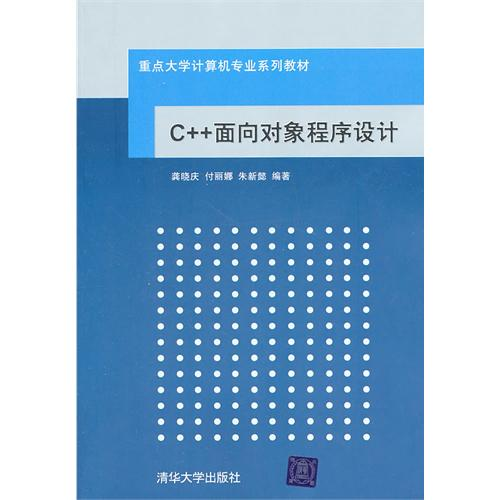
\includegraphics[height=0.4\textheight]{chap00/01textbook.jpg} %
  \end{itemize}
  \stretchoff
\end{frame}

\begin{frame}{课程概况}{参考资料}
  \stretchon
  \begin{itemize}
  \item\hilite<1> {\bfseries 参考资料:}    
    \begin{itemize}
    \item The C++ Programming Language, 4th Edition. Stroustrup,
      Bjarne. Addison-Wesley. 2013.
    \item C++ How to Program, 10th Edition. Paul Deitel, Harvey
      Deitel. Prentice Hall. 2016.
    \item Programming Abstractions in C++. Eric Roberts. Prentice Hall. 2013.
    \end{itemize}
    \centering
    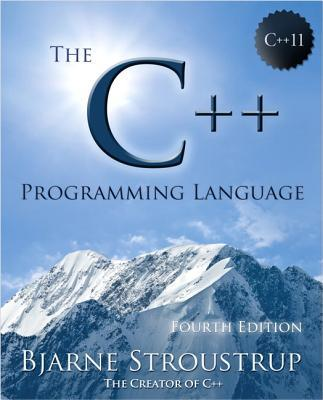
\includegraphics[height=0.35\textheight]{chap00/03programming.jpg} %
    \quad 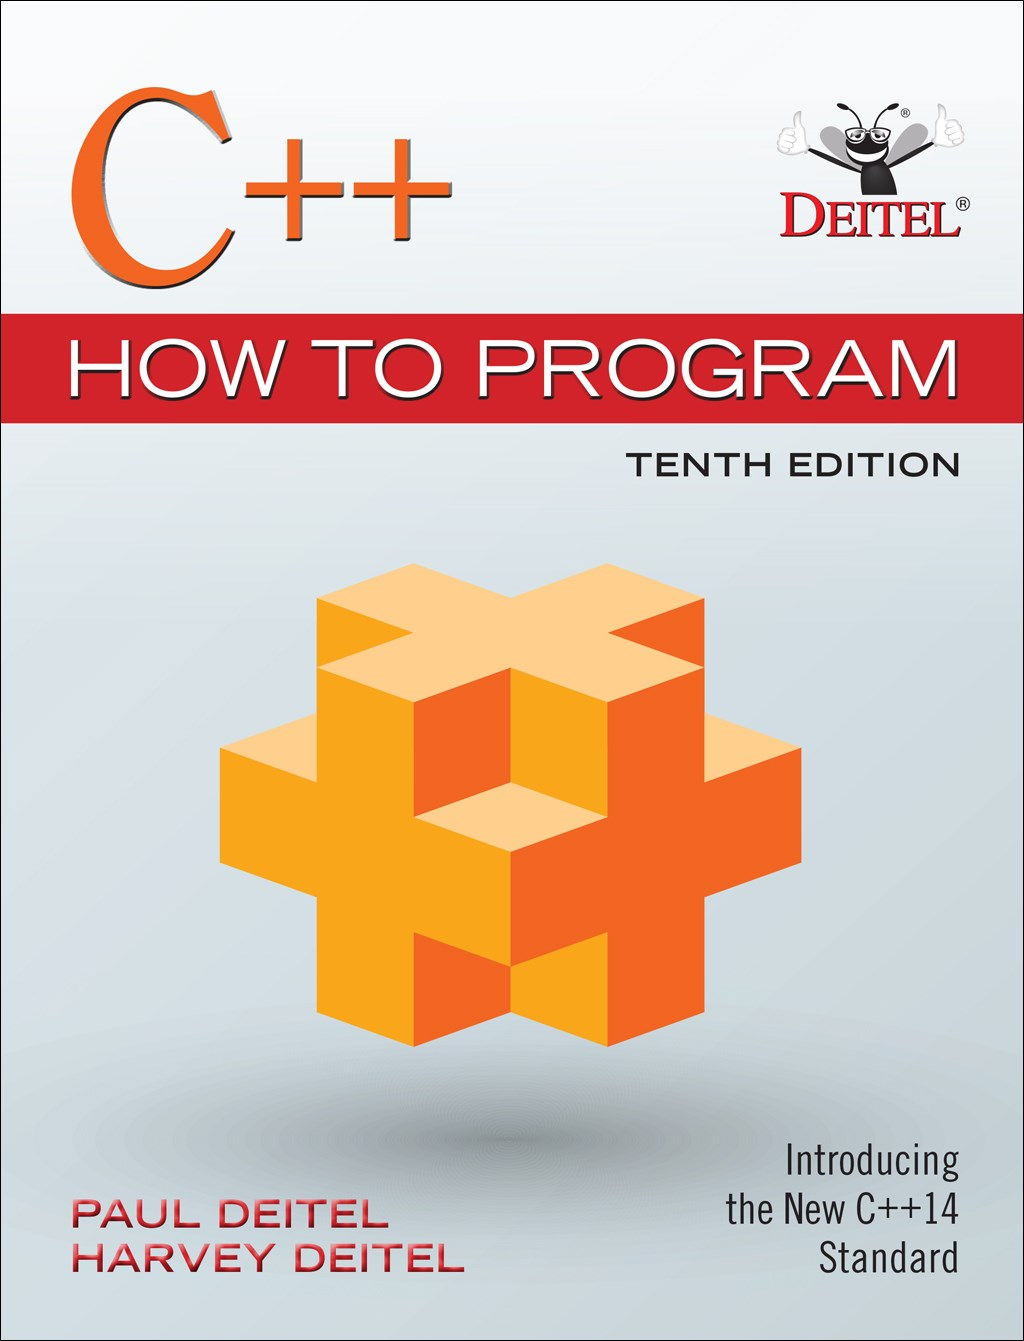
\includegraphics[height=0.35\textheight]{chap00/CHTP.jpg} %
    \quad 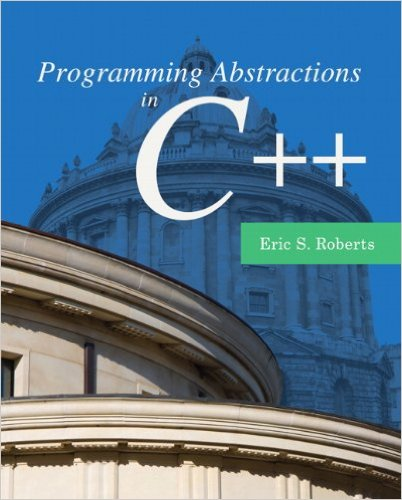
\includegraphics[height=0.35\textheight]{chap00/PAinCPP.jpg} %
  \end{itemize}
  \stretchoff
\end{frame}

\section[要求]{基本要求}\label{sec:chap00-sec03}
\begin{frame}{课程要求}{基本要求}
  \stretchon
  \begin{itemize}
  \item {\bfseries 考勤}(\alert{扣分制度})
    \begin{itemize}
    \item 课堂随机考勤
    \item 实习课随机考勤
    \end{itemize}
  \item  {\bfseries 成绩评定}
    \begin{itemize}
    \item 结业(期末)考试---\alert{70\%}
      \begin{itemize}
      \item 笔试(\alert{闭卷},拟定于XX周)
      \end{itemize}
    \item 平时成绩---\alert{30\%}
      \begin{itemize}
      \item 考勤      
      \item 在线评阅系统成绩(\url{http://202.117.179.201/contest.php?cid=1047})
      \item 大作业(论文分析或采用面向对象方法开发一个实用小软件)
      \end{itemize}
    \end{itemize}
  \end{itemize}
  \stretchoff
\end{frame}

\section[内容]{讲授内容}\label{sec:chap00-sec04}
\begin{frame}{课程内容}{讲授内容}
  \stretchon
  %\renewcommand{\labelenumi}{[\arabic{enumi}]} %
  % \begin{enumerate}
  % \item 第~\chinese{enumi}~章~面向对象基础%
  % \item 第~\chinese{enumi}~章~C++语言概览%
  % \item 第~\chinese{enumi}~章~C++语言基础%    
  % \item 第~\chinese{enumi}~章~复合类型
  % \item 第~\chinese{enumi}~章~函数%
  % \item 第~\chinese{enumi}~章~类和对象%
  % \item 第~\chinese{enumi}~章~对象的初始化、复制和销毁
  % \item 第~\chinese{enumi}~章~运算符重载%
  % \item 第~\chinese{enumi}~章~组合与继承%
  % \item 第~\chinese{enumi}~章~虚函数与多态性%
  % \item 第~\chinese{enumi}~章~模板与泛型编程%
  % \item 第~\chinese{enumi}~章~标准库容器和算法%
  % \item 第~\chinese{enumi}~章~异常处理
  % \end{enumerate}
  % %\renewcommand{\labelenumi}{[\arabic{enumi}]} %
  \begin{enumerate}
  \item 第~1~章~面向对象基础%
  \item 第~2~章~C++语言概览%
  \item 第~3~章~C++语言基础%    
  \item 第~4~章~复合类型
  \item 第~5~章~函数%
  \item 第~6~章~类和对象%
  \item 第~7~章~对象的初始化、复制和销毁
  \item 第~8~章~运算符重载%
  \item 第~9~章~组合与继承%
  \item 第~10~章~虚函数与多态性%
  \item 第~11~章~模板与泛型编程%
  \item 第~12~章~标准库容器和算法%
  \item 第~13~章~异常处理
  \end{enumerate}
  \stretchoff
\end{frame}

\begin{frame}{课程内容}{知识体系}
  \stretchon
  \begin{itemize}
  \item 思维导图
  \end{itemize}
  \centering
    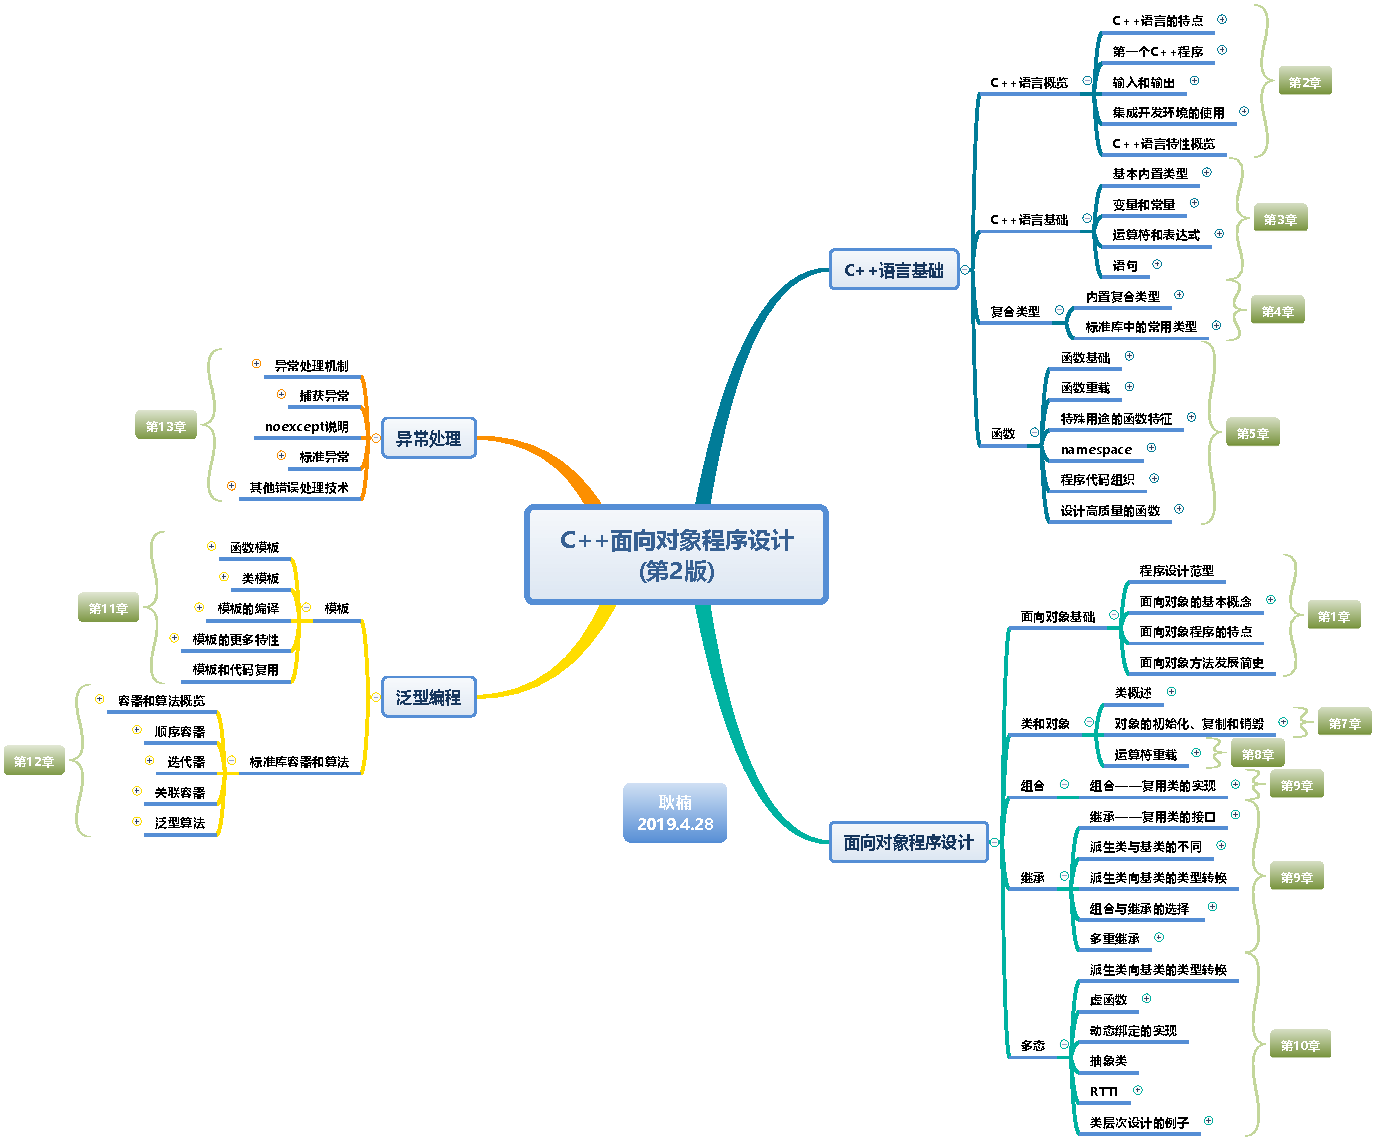
\includegraphics[height=0.8\textheight]{chap00/oopmindmap} %
  \stretchoff
\end{frame}

\begin{frame}{课程内容}{知识体系}
  \stretchon
  \begin{itemize}
  \item 学习路线
  \end{itemize}
  \centering
  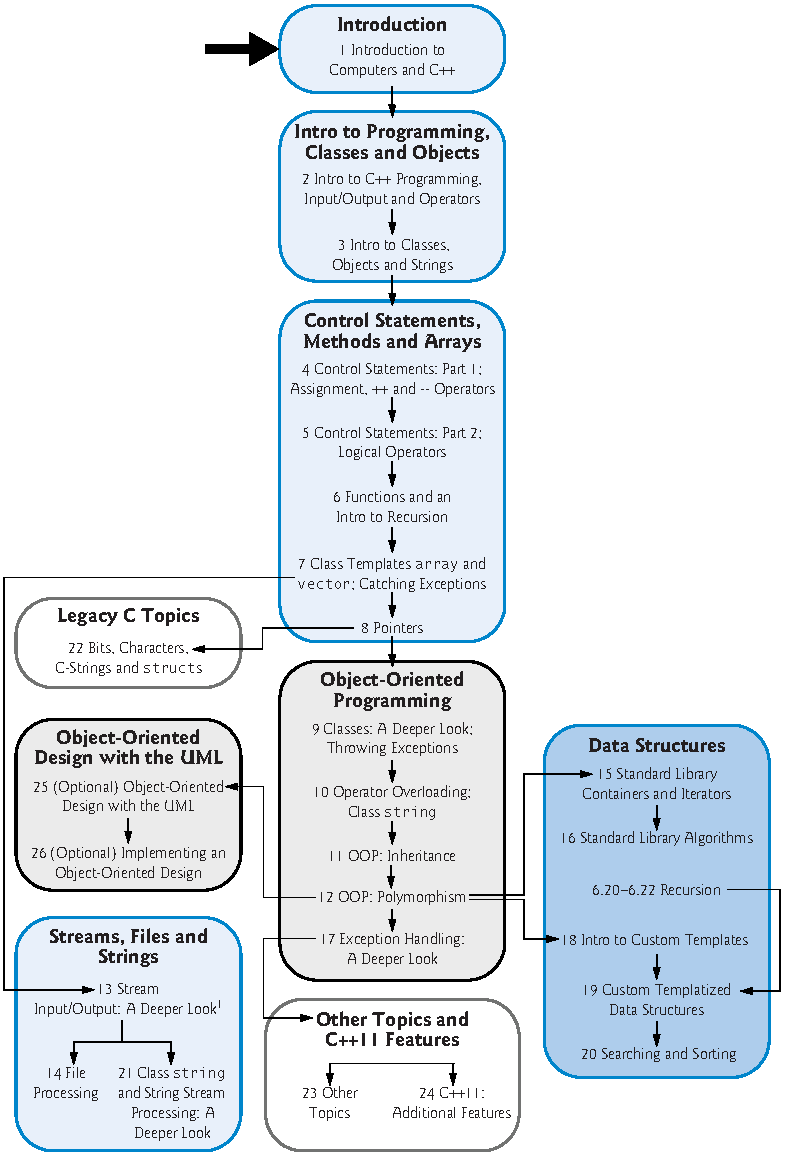
\includegraphics[height=0.8\textheight]{chap00/studyscheme} %
  \stretchoff
\end{frame}

%%%%%%%%%%%%%%%%%%%%%%%%%%%%%% 关于我 %%%%%%%%%%%%%%%%%%%%%%%%%%%%%%%%%%%
\section[关于我]{关于我}
\subsection[联系方式]{联系方式}
\begin{frame}[fragile]{关于我}{联系方式}
  % colour options
  \definecolor{seplinecolour}{HTML}{357f2d} % green
  \definecolor{iconcolour}{HTML}{2f3142} % dark
  \definecolor{textcolour}{HTML}{2f3142} % dark
  \definecolor{jobtitlecolour}{HTML}{474a65} % light dark

  % define some lengths for internal spacing
  \newlength{\seplinewidth} \setlength{\seplinewidth}{2cm}
  \newlength{\seplineheight} \setlength{\seplineheight}{1pt}
  \newlength{\seplinedistance} \setlength{\seplinedistance}{0.3cm}
  \begin{center}
    \begin{tikzpicture}
      % name
      \matrix[every node/.style={anchor=center,font=\huge},anchor=center] (name) {
        \node{耿\hspace{\ccwd}楠}; \\
        \node{\color{jobtitlecolour}\normalsize\textit{教授}}; \\
      };
      % sep line 1
      \node[below=0.3\seplinedistance of name] (hl1) {};
      \draw[line width=\seplineheight,color=seplinecolour] (hl1)++(-\seplinewidth/2,0) -- ++(\seplinewidth,0);
      % contact info
      \matrix [below=\seplinedistance of hl1,%
               column 1/.style={anchor=center,color=iconcolour},%
               column 2/.style={anchor=west}] (contact) {
        \node{\faGlobe}; & \node{\url{http://cie.nwsuaf.edu.cn/}};\\
        \node{\faBuilding}; & \node{信息工程学院};\\ 
        \node{\faEnvelope}; & \node{1234567890@nwafu.edu.cn};\\
        %\node{\faQq}; & \node{970291228};\\
        %\node{\faPhone}; & \node{15829540966}; \\
        \node{\faGithub}; & \node{\url{https://github.com/registor/}}; \\
      };
      %sep line 2
      \node[below=\seplinedistance of contact] (hl2) {};
      \draw[line width=\seplineheight,color=seplinecolour] (hl2)++(-\seplinewidth/2,0) -- ++(\seplinewidth,0);
      % interests
      \matrix [below=\seplinedistance of hl2,
         every node/.style={anchor=center,font=\LARGE}]
         (interests) {
        \node{\faCode}; & \node{\faCoffee}; &
        \node{\faLock}; & \node{\faWrench}; &
        \node{\faCameraRetro}; \\
      };
      
    \end{tikzpicture}
  \end{center}
\end{frame}
%%%%%%%%%%%%%%%%%%%%%%%%%%%%%%%%%%%%%%%%%%%%%%%%%%%%%%%%%%%%%%%%%%%%%%%%%%

%%% Local Variables: 
%%% mode: latex
%%% TeX-master: "../main.tex"
%%% End: 
 % 绪论
  \or % 第1章
    \lecture{绪论}{lec:chap01}
\section[基本特性]{对象、类及其特性}\label{sec:chap01-sec01}
%%%%%%%%%%%%%%%%%%%%%%%%%%%%%% 对象、类及其特性 %%%%%%%%%%%%%%%%%%%%%%%%%%%%%%%%%%
\begin{frame}{基本特性}{普通定义}
  \stretchon
  \begin{itemize}
  \item 对象
    \begin{itemize}
    \item 目标
    \item 恋爱的对方
    \item 描写或写实的人或物
    \end{itemize}
  \item Object
    \begin{itemize}
    \item Something perceptible by one or more of the senses,
      especially by vision or touch; a material thing
    \item The purpose or goal of a specific action
    \item \ldots\ldots
    \end{itemize}
  \end{itemize}
  \stretchoff
\end{frame}

\begin{frame}{基本特性}{课程定义}
  \stretchon
  \begin{itemize}
  \item 对象(现实世界)
    \begin{itemize}
    \item 现实世界中的某个具体的事物(实物或实体)
    \item 一个封装了属性(attribute)与行为(behavior)的实体
    \end{itemize}
  \item 对象(计算机世界)---\alert{数据结构}
    \begin{itemize}
    \item 数据域
    \item 方法
    \item 相互作用关系
    \end{itemize}
  \end{itemize}
  \stretchoff
\end{frame}

\begin{frame}{基本特性}{对象实例:树}
  \stretchon
  \begin{itemize}
  \item 属性
    \begin{itemize}
    \item 树干树枝、树叶、树龄、纹理、荷尔蒙\ldots\ldots
    \end{itemize}
  \end{itemize}
  \centering
  %\begin{center}
    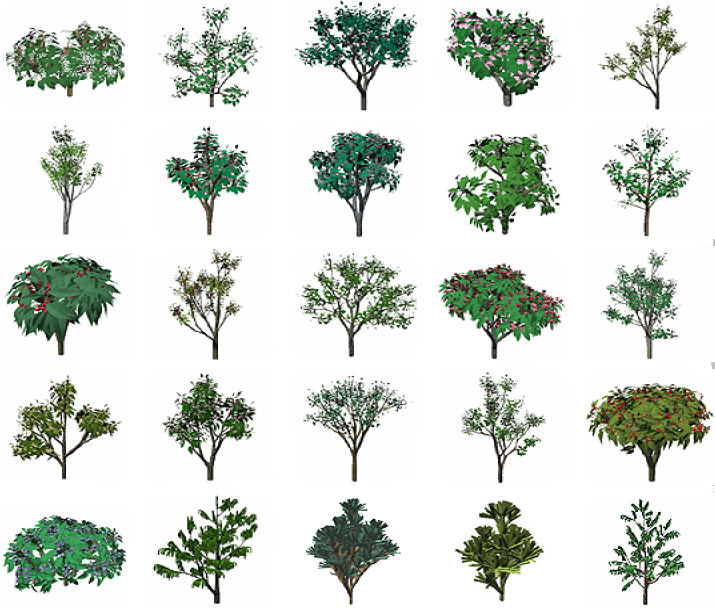
\includegraphics[height=0.6\textheight]{chap01/01trees} %
    % \end{center}
  \stretchoff
\end{frame}

\begin{frame}{基本特性}{对象实例:树}
  \stretchon
  \begin{itemize}
  \item 方法(行为、操作)
    \begin{itemize}
    \item 生长、四季变化、修剪、运动、叶枝摩擦、声音\ldots\ldots
    \end{itemize}
  \end{itemize}
  \vspace{-1ex}
  \centering
  %\begin{center}
    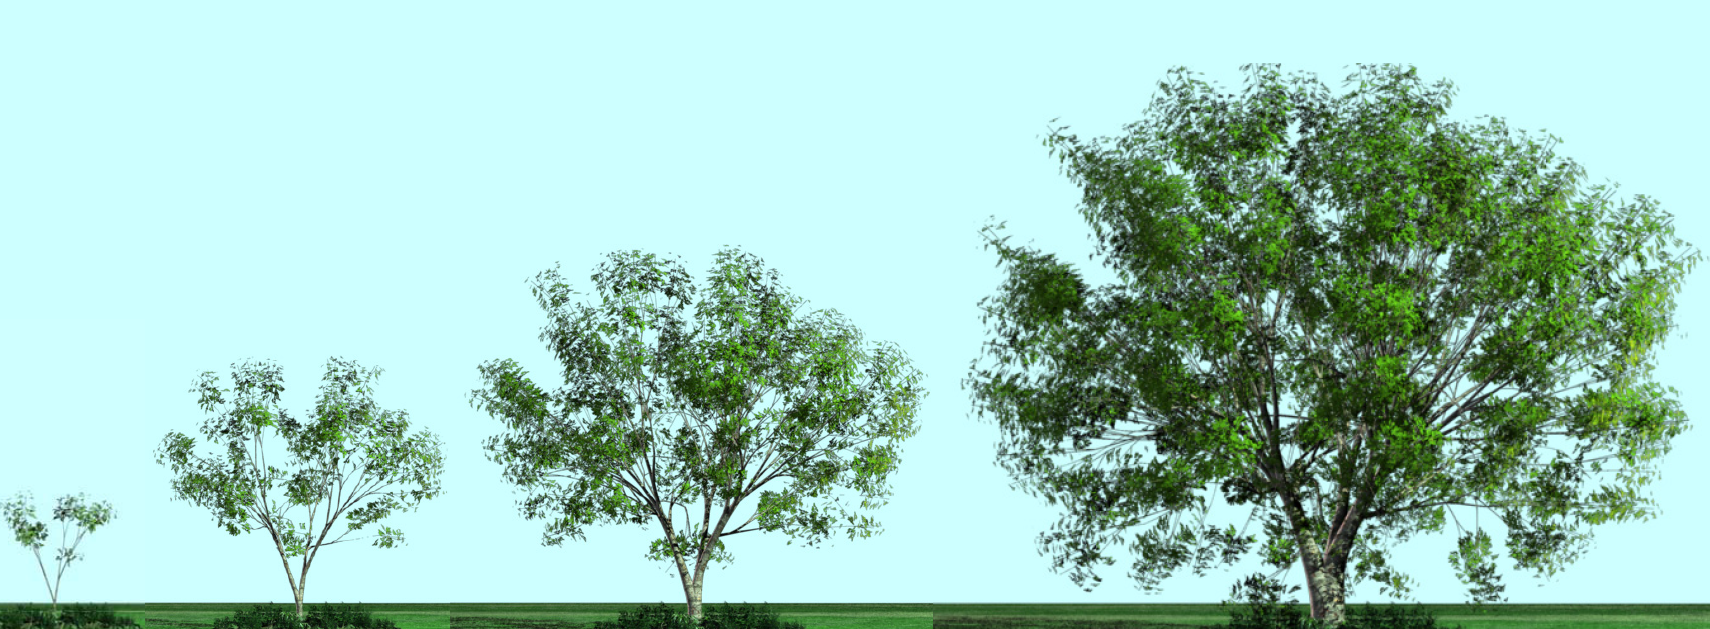
\includegraphics[height=0.25\textheight]{chap01/02treesgrow} \\[1ex]%
    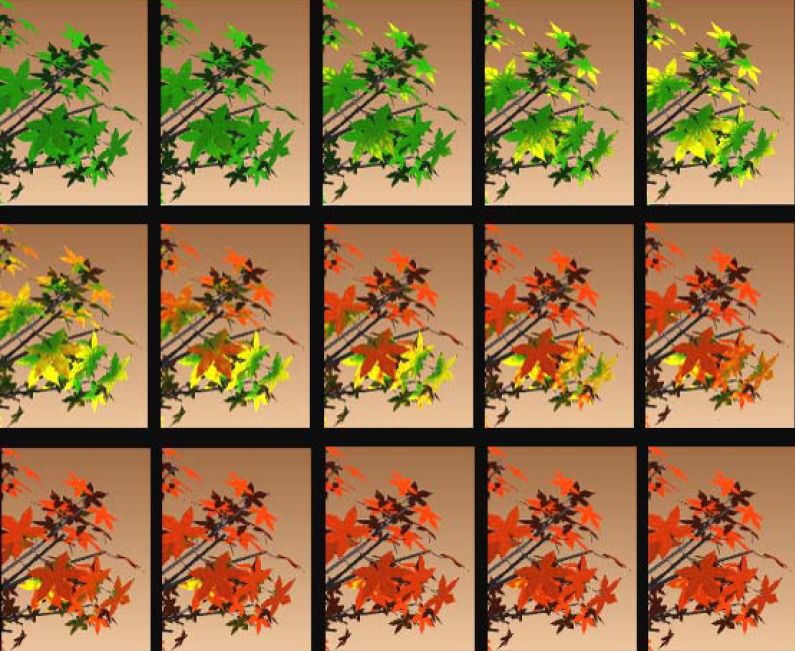
\includegraphics[height=0.45\textheight]{chap01/03treesseason} %
  %\end{center}
  \stretchoff
\end{frame}

\begin{frame}{基本特性}{对象实例:俄罗斯方块}
  \stretchon
  \begin{itemize}
  \item 属性
    \begin{itemize}
    \item 颜色,四个方块的布局,大小,位置,速度,\ldots\ldots
    \end{itemize}
  \item 行为
    \begin{itemize}
    \item 平移,旋转,加速,碰撞检测,显示,\ldots\ldots
    \end{itemize}
  \end{itemize}
  \centering
  %\begin{center}
    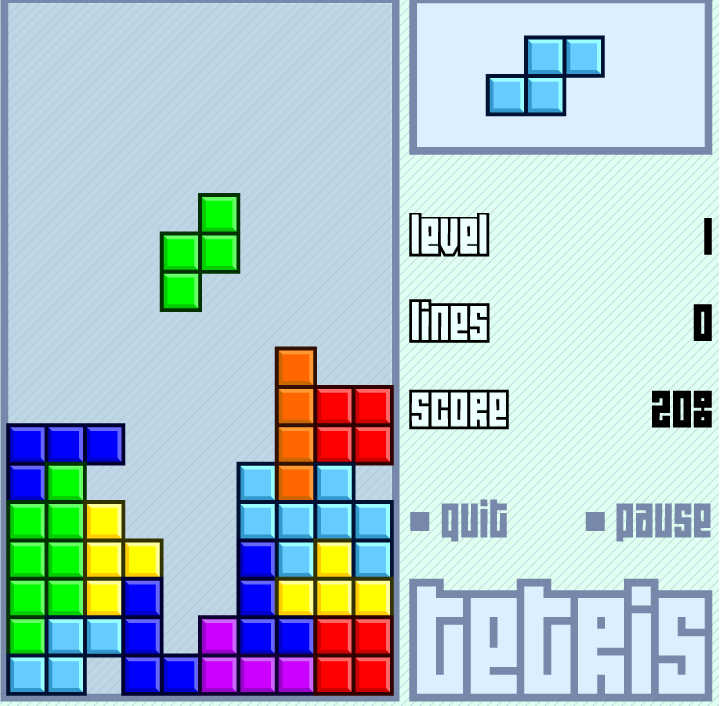
\includegraphics[width=0.35\textwidth]{chap01/04tetrogame} \qquad%
    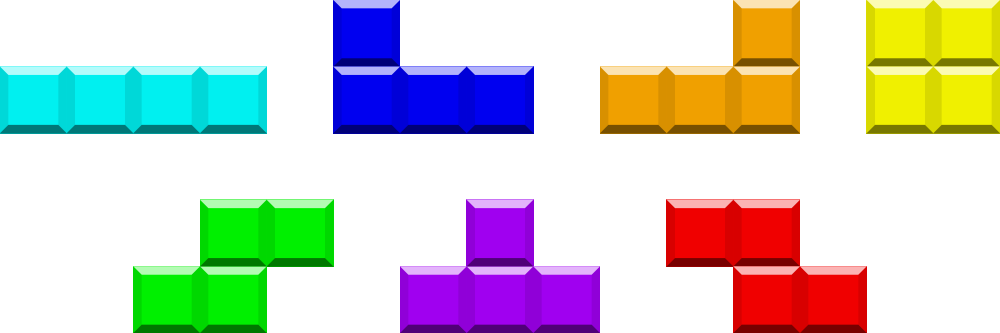
\includegraphics[width=0.55\textwidth]{chap01/05tetroobj} %
  %\end{center}
  \stretchoff
\end{frame}

\begin{frame}[t, fragile]{基本特性}{消息(message)}
  \begin{itemize}
  \item 类\\
    \begin{minipage}{0.8\linewidth}
      \begin{cpptt}
CTetromino{
  |\textbf{\textcolor{blue}{属性:}}颜色,四个方块的布局,大小,位置,速度,$\cdots$|
  |\textbf{\textcolor{blue}{行为:}}平移,旋转,加速,碰撞检测,显示,$\cdots$|
};
      \end{cpptt}
    \end{minipage}
  \item 类对象\\
    \begin{minipage}{0.8\linewidth}
      \begin{cppcode}
CTetromino I, J, L, O, S, T, Z;
      \end{cppcode}
    \end{minipage}
  \item 操作对象
    \begin{itemize}
    \item 向对象发送消息
    \item 通过调用对象的操作实现
    \end{itemize}
    \begin{minipage}{0.5\linewidth}
      \begin{cpptt}
CTetromino S(|\textcolor{green}{绿色}|, 01101100);
S.|平移|(-1, 0);
      \end{cpptt}
    \end{minipage} \qquad
    \onslide<2->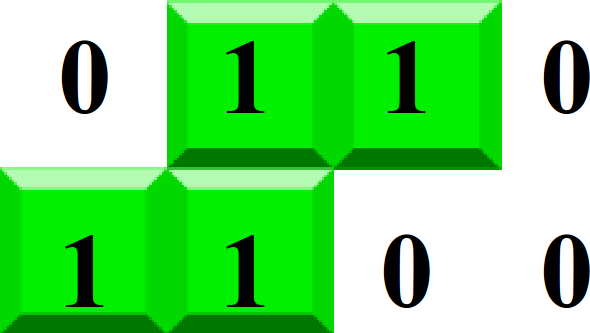
\includegraphics[width=0.12\textwidth]{chap01/06tetromove}\qquad%
    \onslide<1>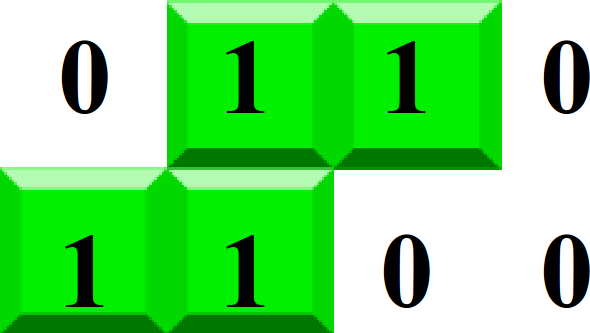
\includegraphics[width=0.12\textwidth]{chap01/06tetromove}%
  \end{itemize}
\end{frame}

\begin{frame}{基本特性}{数据抽象(Data abstraction)}
  \stretchon
  \begin{itemize}
  \item 抽象
    \begin{itemize}
    \item 抽取共性
    \item 问题空间的事物 $\Rightarrow$ 解空间的面向对象的概念
    \end{itemize}
  \item 示例1:两栖动物\\
    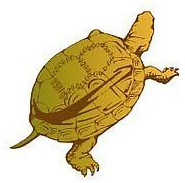
\includegraphics[width=0.2\textwidth]{chap01/07abstraction01} \qquad%
    
\includegraphics[width=0.2\textwidth]{chap01/07abstraction02} \qquad%
    
\includegraphics[width=0.2\textwidth]{chap01/07abstraction03} %
  \item 示例2:斑马\\
    \centering
    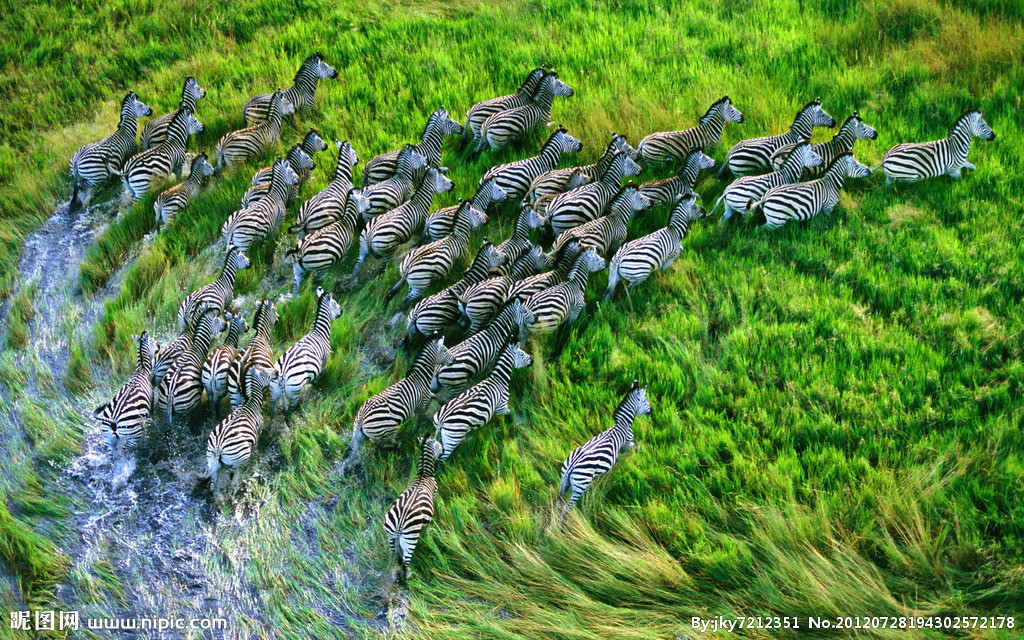
\includegraphics[width=0.3\textwidth]{chap01/07abstraction04}    
  \end{itemize}
  \stretchoff
\end{frame}

\begin{frame}{基本特性}{封装性(Encapsulation)}
  \stretchon
  \begin{itemize}
  \item 对象的\alert{属性}和\alert{服务}结合成一个\alert{独立的系统单
      位}
  \item 隐蔽对象的\alert{内部细节}
  \item 保留有限的\alert{对外接口}
  \item \alert{代码安全性}
  \item 示例:\\
    \centering
    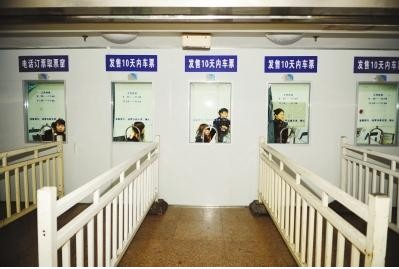
\includegraphics[width=0.4\textwidth]{chap01/08encap01}\qquad%
    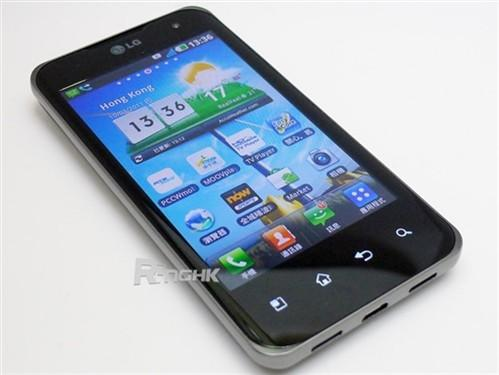
\includegraphics[width=0.4\textwidth]{chap01/08encap02}
  \end{itemize}
  \stretchoff
\end{frame}

\begin{frame}{基本特性}{类和对象的UML图示}
  \begin{columns}[c]
    \begin{column}{0.4\textwidth}
      \begin{spacing}{1.5}
      \begin{itemize}
      \item 类(三栏矩形)
        \begin{itemize}
        \item 类名
        \item 属性
        \item 操作
        \item 对外可见性
          \begin{itemize}
          \item ``+''---公有
          \item ``-''---私有
          \end{itemize}
        \end{itemize}
      \item 对象(矩形)
        \begin{itemize}
        \item 对象名称
        \item 类型
        \item 属性值
        \end{itemize}
      \end{itemize}
      \end{spacing}
    \end{column}
    \begin{column}{0.6\textwidth}
      \tiny
      \centering
      \begin{tikzpicture}
        \begin{class}[text width=0.2\textwidth]{类名}{0, 0}
          \attribute{- 属性1}
          \attribute{- 属性2}

          \operation{+ 操作1()}
          \operation{+ 操作2()}
        \end{class}
        
        \begin{class}[text width=0.7\textwidth]{Circle}{0, -3}
          \attribute{- radius : double}
          \attribute{- center\_x : int}
          \attribute{- center\_y : int}
          
          \operation{+ area() : double}
          \operation{+ perimeter() : double}
          \operation{+ move(in newx : int, in newy : int) : void}
          \operation{+ scale(in factor : double) : void}
        \end{class}
      \end{tikzpicture}
    \end{column}
  \end{columns}
\end{frame}

\begin{frame}{基本特性}{类和对象的UML图示}
  \begin{columns}[c]
    \begin{column}{0.4\textwidth}
      \begin{spacing}{1.5}
      \begin{itemize}
      \item 类(三栏矩形)
        \begin{itemize}
        \item 类名
        \item 属性
        \item 操作
        \item 对外可见性
          \begin{itemize}
          \item ``+''---公有
          \item ``-''---私有
          \end{itemize}
        \end{itemize}
      \item 对象(矩形)
        \begin{itemize}
        \item 对象名称
        \item 类型
        \item 属性值
        \end{itemize}
      \end{itemize}
      \end{spacing}
    \end{column}
    \begin{column}{0.6\textwidth}
      \tiny
      \centering
      \begin{tikzpicture}
        \begin{class}[text width=0.2\textwidth]{类名}{0, 0}
          \operation{+ 操作1()}
          \operation{+ 操作2()}
        \end{class}
        
        \begin{class}[text width=0.7\textwidth]{Circle}{0, -3}
          \operation{+ area() : double}
          \operation{+ perimeter() : double}
          \operation{+ move(in newx : int, in newy : int) : void}
          \operation{+ scale(in factor : double) : void}
        \end{class}
      \end{tikzpicture}
    \end{column}
  \end{columns}
\end{frame}

\begin{frame}{基本特性}{类和对象的UML图示}
  \begin{columns}[c]
    \begin{column}{0.4\textwidth}
      \begin{spacing}{1.5}
      \begin{itemize}
      \item 类(三栏矩形)
        \begin{itemize}
        \item 类名
        \item 属性
        \item 操作
        \item 对外可见性
          \begin{itemize}
          \item ``+''---公有
          \item ``-''---私有
          \end{itemize}
        \end{itemize}
      \item 对象(矩形)
        \begin{itemize}
        \item 对象名称
        \item 类型
        \item 属性值
        \end{itemize}
      \end{itemize}
      \end{spacing}
    \end{column}
    \begin{column}{0.6\textwidth}
      \tiny
      \centering
      \begin{tikzpicture}
        \begin{class}[text width=0.2\textwidth]{类名}{0, 0}          
        \end{class}        
        \begin{class}[text width=0.2\textwidth]{Circle}{3, 0}          
        \end{class}
      
        \begin{object}[text width=0.3\textwidth]{对象名称}{0, -3}
          \instanceOf{类名}
          \attribute{属性1=值1}
          \attribute{属性2=值2}
        \end{object}

        \begin{object}[text width=0.4\textwidth]{cobj}{3, -3}
          \instanceOf{Circle}
          \attribute{radius : double = 2.7}
          \attribute{center\_x : int = 10}
          \attribute{center\_y : int = 20}
        \end{object}
      \end{tikzpicture}
    \end{column}
  \end{columns}
\end{frame}

\begin{frame}{基本特性}{继承性(Inheritance)}
  \stretchon
  \begin{itemize}
  \item 一般类 $\Rightarrow$ 特殊类(\alert{具备全部属性与行为})
  \item \alert{代码重用}
  \item 示例1:\\
    \centering
    \scalebox{0.5}{
    \begin{tikzpicture}
      \path[mindmap, text=white,%concept color=black,text=white]
               root concept/.append style={concept color=black},
               level 1 concept/.append style={level distance=60, sibling angle=90}
           ]
      node[concept]{马}
      [clockwise from=-45]
      child[concept color=green!50!black] {
        node[concept] {蒙古马}
      }
      child[concept color=blue] {
        node[concept] {斑马}
      };
    \end{tikzpicture}
    }\\
    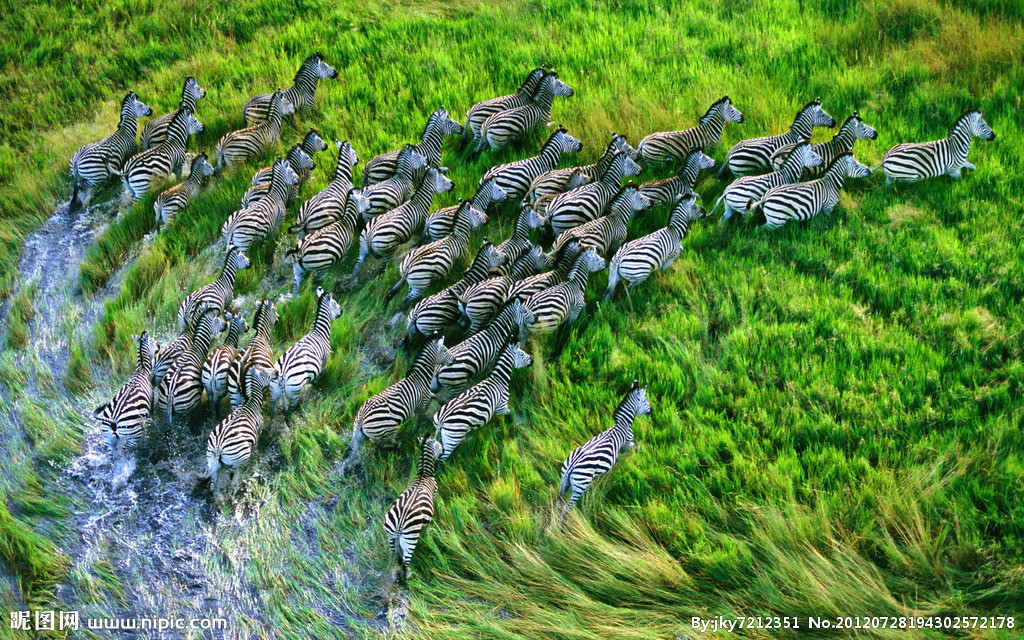
\includegraphics[width=0.4\textwidth]{chap01/09inherit01}\qquad%
    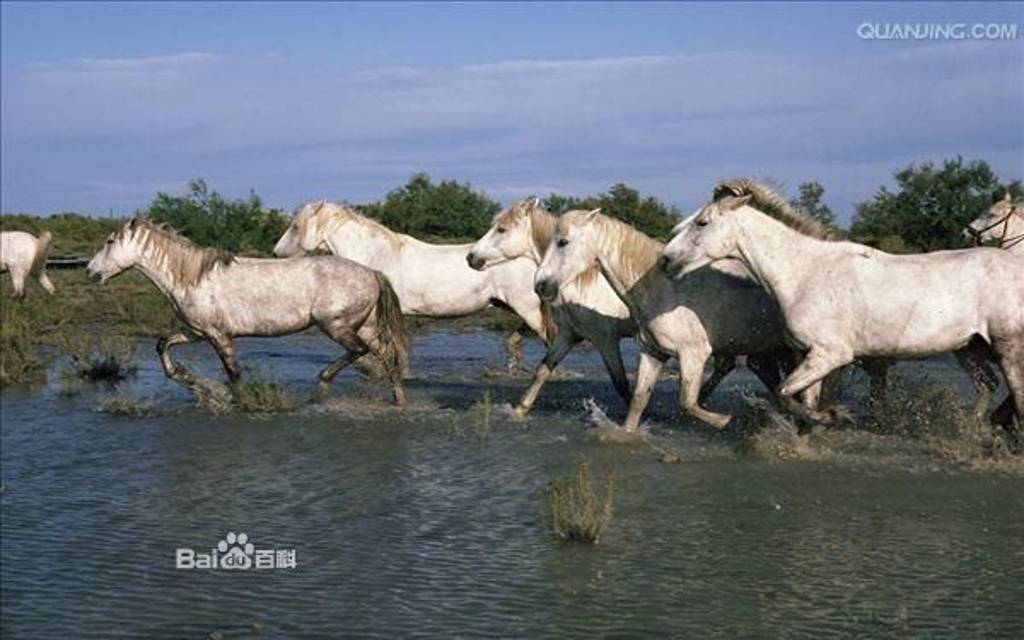
\includegraphics[width=0.4\textwidth]{chap01/09inherit02}
  \end{itemize}
  \stretchoff
\end{frame}

\begin{frame}[fragile]{基本特性}{继承性(Inheritance)}
  \begin{itemize}
  \item 示例2(伪代码):\\
    \begin{minipage}{0.8\linewidth}
      \begin{cpptt}
Animal|类|{
    Animal|类|(const string& name) : name(name) {}
    virtual string talk() = 0;
    const string name;
};
      \end{cpptt}
    \end{minipage}\\
    \begin{minipage}{0.8\linewidth}
      \begin{cpptt}
Cat|类| : Animal|类|{
    Cat|类|(const string& name): Animal|类|(name) {}
    string talk() { return "喵喵!"; }
};
      \end{cpptt}
    \end{minipage}
    \begin{minipage}{0.8\linewidth}
      \begin{cpptt}
Dog|类| : Animal|类|{
    Dog|类|(const string& name): Animal|类|(name) {}
    string talk() { return "汪汪!"; }
};
      \end{cpptt}
    \end{minipage}  
  \end{itemize}
\end{frame}

\begin{frame}{基本特性}{继承性(Inheritance)}
  \stretchon
  \begin{itemize}
  \item 类的继承
  \end{itemize}
  %\stretchon
  \tiny
  %\centering
  \qquad\qquad\qquad\qquad
  \begin{tikzpicture}
    \begin{class}[text width=0.2\textwidth]{父类}{0, 0}
      \operation{+ 操作1()}
      \operation{+ 操作2()}
    \end{class}
    \begin{class}[text width=0.2\textwidth]{子类1}{-2, -1.5}
      \inherit{父类}
      \operation{+ 操作3()}
    \end{class}
    \begin{class}[text width=0.2\textwidth]{子类2}{2, -1.5}
      \inherit{父类}
      \operation{+ 操作4()}
    \end{class}
  
    \begin{class}[text width=0.2\textwidth]{A}{-2, -3}
      \operation{+ 操作1()} \operation{+ 操作2()}
    \end{class}
    \begin{class}[text width=0.2\textwidth]{B}{-2, -4.5}
      \inherit{A}
      % \operation{+ 操作3()}
    \end{class}

    \begin{class}[text width=0.2\textwidth]{Rectangle}{2, -3}
      \attribute{- width}
      \attribute{- length}
      \operation{+ area()}
      \operation{+ perimeter()}
      \operation{+ scale()}
    \end{class}
    \begin{class}[text width=0.2\textwidth]{Square}{2, -5.3}
      \inherit{Rectangle}
      \operation{+ scale()}
    \end{class}
  \end{tikzpicture}
  \stretchoff
\end{frame}

\begin{frame}{基本特性}{继承性(Inheritance)}
  \stretchon
  \begin{itemize}
  \item 类的继承
  \end{itemize}
  \tiny
  \centering
  %\qquad\qquad\qquad\qquad\qquad\qquad
  \begin{tikzpicture}
    \begin{class}[text width=0.2\textwidth]{电话机}{0, 0}
      \operation{+ 拨出()}
      \operation{+ 接听()}
    \end{class}
    
    \begin{class}[text width=0.2\textwidth]{固定话机}{-2, -1.5}
      \inherit{电话机}
      %\operation{+ 操作3()}
    \end{class}
    
    \begin{class}[text width=0.2\textwidth]{手机}{2, -1.5}
      \inherit{电话机}
      \operation{+ 发送短信()}
      \operation{+ 接收短信()}
    \end{class}

    \begin{class}[text width=0.2\textwidth]{音乐手机}{0, -3.5}
      \inherit{手机}
      \operation{+ 播放音乐()}
    \end{class}
    
    \begin{class}[text width=0.2\textwidth]{3G手机}{4, -3.5}
      \inherit{手机}
      \operation{+ 网络电视()}
      \operation{+ 收发电邮()}
    \end{class}  
    
  \end{tikzpicture}
  \stretchoff
\end{frame}

\begin{frame}[fragile]{基本特性}{多态性(Polymorphism)}
  %\stretchon
  \begin{itemize}
  \item 在\alert{一般类}中定义的属性或行为,被\alert{特殊类继承}之后,
    可以具有不同的数据类型或表现出\alert{不同的行为}\\
    \begin{minipage}{0.8\linewidth}
      \begin{cpptt}
Animal|类| *animalCat = new Cat|类|("爱丽丝");
Animal|类| *animalDog = new Dog|类|("旺财");

cout << animalCat->name << ": " << animalCat->talk() << endl;
cout << animalDog->name << ": " << animalDog->talk() << endl;
      \end{cpptt}
    \end{minipage}
  \end{itemize}
  
  \begin{center}
    \begin{tikzpicture}[font=\scriptsize]
      \begin{class}[text width=0.2\textwidth]{Animal}{0, 0}
        \attribute{- name}
        \operation{+ talk()}
      \end{class}
    
    \begin{class}[text width=0.2\textwidth]{Cat}{-2, -2.5}
      \inherit{Animal}
      \attribute{- name}
      \operation{+ talk()}
    \end{class}
    
    \begin{class}[text width=0.2\textwidth]{Dog}{2, -2.5}
      \inherit{Animal}
      \attribute{- name}
      \operation{+ talk()}
    \end{class}
  \end{tikzpicture}
\end{center}
  %\stretchoff
\end{frame}

\begin{frame}{基本特性}{多态性(Polymorphism)}
  \stretchon
  \begin{itemize}
  \item 形状类
  \end{itemize}  
  \centering%begin{center}
    \begin{tikzpicture}[font=\scriptsize]
      \begin{class}[text width=0.2\textwidth]{shape}{0, 0}
        \attribute{-center}        
        \operation{+area()}
        \operation{+perimeter()}
        \operation{+draw()}
        \operation{+erase()}
      \end{class}
    
    \begin{class}[text width=0.2\textwidth]{circle}{-3.5, -3.5}
      \inherit{shape}
      \attribute{-radius}
      \operation{+area()}
      \operation{+perimeter()}
    \end{class}
    
    \begin{class}[text width=0.2\textwidth]{rectangle}{0, -3.5}
      \inherit{shape}
      \attribute{-width}
      \attribute{-height}
      \operation{+area()}
      \operation{+perimeter()}
    \end{class}

    \begin{class}[text width=0.2\textwidth]{triangle}{3.5, -3.5}
      \inherit{shape}
      \attribute{-a}
      \attribute{-b}
      \attribute{-c}
      \operation{+area()}
      \operation{+perimeter()}
    \end{class}
  \end{tikzpicture}
%\end{center}
  \stretchoff
\end{frame}

\begin{frame}{基本特性}{类之间的关系}
  %\stretchon
  \begin{itemize}
  \item 组合
    \begin{itemize}
    \item 整体和部分关系
    \item 同时存在
    \item 同时销毁
    \end{itemize}
  \end{itemize}
  \vspace{4ex}
  \centering%begin{center}
  \begin{tikzpicture}[font=\scriptsize]
    \begin{class}[text width=0.1\textwidth]{计算机}{0, 0}
    \end{class}

    \begin{class}[text width=0.1\textwidth]{显示器}{3, 0}
    \end{class}

    \begin{class}[text width=0.1\textwidth]{主机}{-3, 0}
    \end{class}

    \begin{class}[text width=0.1\textwidth]{键盘}{-2, -2.5}
    \end{class}

    \begin{class}[text width=0.1\textwidth]{鼠标}{2, -2.5}
    \end{class}
    
    \composition{计算机}{}{1..*}{显示器}
    \composition{计算机}{}{1}{主机}
    \composition{计算机}{}{0..1}{鼠标}
    \composition{计算机}{}{1}{键盘}
  \end{tikzpicture}
  %\stretchoff
\end{frame}

\begin{frame}{基本特性}{类之间的关系}
  %\stretchon
  \begin{itemize}
  \item 聚合
    \begin{itemize}
    \item 包含关系
    \item 共享成员
    \item \alert{组合的泛化}
    \end{itemize}
  \end{itemize}
  \vspace{4ex}
  \centering%begin{center}
  \begin{tikzpicture}[font=\scriptsize]
    \begin{class}[text width=0.1\textwidth]{球队}{0, 0}
    \end{class}

    \begin{class}[text width=0.1\textwidth]{球员}{4, 0}
    \end{class}

    \begin{class}[text width=0.1\textwidth]{主教练}{4, -2.5}
    \end{class}
    
    \aggregation{球队}{}{*}{球员}
    \aggregation{球队}{}{1}{主教练}
  \end{tikzpicture}
  %\stretchoff
\end{frame}

\begin{frame}{基本特性}{类之间的关系}
  %\stretchon
  \begin{itemize}
  \item 关联
    \begin{itemize}
    \item 消息传递链
    \item \alert{聚合的泛化}
    \end{itemize}
  \end{itemize}
  \vspace{6ex}
  \centering%begin{center}
  \begin{tikzpicture}[font=\scriptsize]
    \begin{class}[text width=0.1\textwidth]{公司}{0, 0}
    \end{class}

    \begin{class}[text width=0.1\textwidth]{员工}{6, 0}
    \end{class}
    
    \association[工作]{公司}{雇主}{0..1}{员工}{1..*}{雇员}
  \end{tikzpicture}
  %\stretchoff
\end{frame}

\begin{frame}{基本特性}{类之间的关系}
  %\stretchon
  \begin{itemize}
  \item 依赖
    \begin{itemize}
    \item 短时使用关系
    \item \alert{非永久关系}
    \end{itemize}
  \end{itemize}
  \vspace{6ex}
  \centering%begin{center}
  \begin{tikzpicture}[font=\scriptsize]
    \begin{class}[text width=0.1\textwidth]{Word文档}{0, 0}
    \end{class}

    \begin{class}[text width=0.2\textwidth]{打印机}{4, 0}
      \operation{+打印()}
    \end{class}
    
    \unidirectionalAssociation{Word文档}{}{}{打印机}
  \end{tikzpicture}
  %\stretchoff
\end{frame}



%%%%%%%%%%%%%%%%%%%%%%%%%%%%%%%%%%%%%%%%%%%%%%%%%%%%%%%%%%%%%%%%%%%%%%%%%%

\section[是什么?]{什么是面向对象程序设计}\label{sec:chap01-sec02}
%%%%%%%%%%%%%%%%%%%%%%%%%%%%%% 什么是面向对象程序设计 %%%%%%%%%%%%%%%%%%%%%%%%%%%%%%%
\begin{frame}{是什么?}{什么是面向对象程序设计}
  \stretchon
  \begin{itemize}
  \item 使用\alert{对象}去设计程序编写代码的一种方法
    \begin{itemize}
    \item 数据抽象
    \item 信息隐藏
    \item 代码重用
    \end{itemize}
  \end{itemize}
  
  \centering
  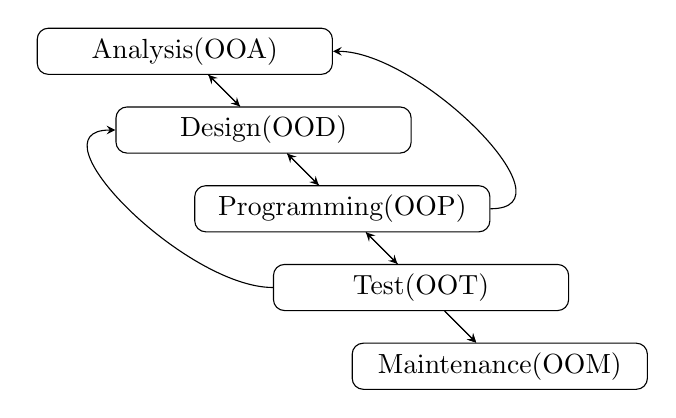
\begin{tikzpicture}[node distance=2.5cm, auto, >=stealth]
    % nodes
    \node[block] (ooa) {Analysis(OOA)};
    \node[block] (ood) [right of=ooa,below of=ooa, node
    distance=1cm] {Design(OOD)};
    \node[block] (oop) [right of=ood,below of=ood, node distance=1cm]
    {Programming(OOP)};
    \node[block] (oot) [right of=oop,below of=oop, node
    distance=1cm] {Test(OOT)};        
    \node[block] (oom) [right of=oot,below of=oot, node
    distance=1cm] {Maintenance(OOM)};

    \draw[->] (ooa) -- (ood);
    \draw[->] (ood) -- (ooa);
        
    \draw[->] (ood) -- (oop);
    \draw[->] (oop) -- (ood);

    \draw[->] (oop) -- (oot);
    \draw[->] (oot) -- (oop);

    \draw[->] (oot) -- (oom);
    \draw[->] (oot) -- (oom);

    \draw[->] (oop.east) to  [out=0,in=0] (ooa.east);
        
    \draw[->] (oot.west)  to  [out=180,in=180] (ood.west);
  \end{tikzpicture}
  \stretchoff
\end{frame}
%%%%%%%%%%%%%%%%%%%%%%%%%%%%%%%%%%%%%%%%%%%%%%%%%%%%%%%%%%%%%%%%%%%%%%%%%%

\section[为什么?]{为何学习面向对象程序设计}\label{sec:chap01-sec03}
%%%%%%%%%%%%%%%%%%%%%%%%%%%%% 为何学习面向对象程序设计 %%%%%%%%%%%%%%%%%%%%%%%%%%%%%%
\begin{frame}{为什么?}{为何学习面向对象程序设计}
  \stretchon
  \begin{itemize}
  \item 过程式程序设计
    \begin{itemize}
    \item 数据和过程分离,可维护性与可重用性差
    \item 不适于大型程序开发
    \end{itemize}
  \item 面向对象程序设计
    \begin{itemize}
    \item 现实世界的直接模拟
    \item 可重用性好,可维护性好
    \item 适合大型程序开发
    \end{itemize}
  \end{itemize}
  \stretchoff
\end{frame}
%%%%%%%%%%%%%%%%%%%%%%%%%%%%%%%%%%%%%%%%%%%%%%%%%%%%%%%%%%%%%%%%%%%%%%%%%%

\section[发展史]{面向对象程序设计语言发展史}\label{sec:chap01-sec04}
%%%%%%%%%%%%%%%%%%%%%%%%%%%% 面向对象程序设计语言发展史 %%%%%%%%%%%%%%%%%%%%%%%%%%%%%%
\begin{frame}[fragile]{发展史}{族谱}
  \stretchon
  \begin{itemize}
  \item 族谱(Family tree)    
  \end{itemize}
  \centering
  \scalebox{0.7}{
  \tikzset{box/.style={rectangle, draw=black, rounded corners}}
  \tikzset{boxgreen/.style={rectangle, draw=black, rounded corners,fill=green}} 
  \begin{tikzpicture}%[scale=\s, every node/.style={scale=\s}]
    \node[box] (asm) {Assembler};
    \node[box] (for) [right=0.5 of asm] {Fortran};
    \node[box] (alg)  [right=0.5  of for] {Algol};
    \node[box] (bcp)  [right=0.5  of alg] {BCPL};
    \node[box] (pas)  [above=1  of bcp] {Pascal};
    \node[boxgreen] (sim) [below=1 of bcp] {Simula};
    \node[box] (c) [right=0.5 of bcp] {C};
    \node[box] (cpp) [right=0.5 of c] {C++};
    \node[box] (cpp0x) [right=0.5 of cpp] {C++0x};
    \node[box] (opas) [above=1 of cpp0x, right=3.1 of pas] {Object Pascal};
    \node[boxgreen] (lisp) [below=2.5 of alg] {Lisp};
    \node[boxgreen] (smt) [right=2.5 of lisp] {Smalltalk};
    \node[box] (jar) [below=2.5 of cpp0x, right=0.8 of smt] {Java};
    \node (endmain)  [right=0.5  of cpp0x] {};
    \node (endopas)  [right=0.5 of opas] {};
    \node (endjava)  [right=0.5  of jar] {};

    \draw[->] (asm) -- (for);
    \draw[->] (for) -- (alg);
    \draw[->] (alg) -- (bcp);
    \draw[->] ([xshift=0.2em]alg.east) |- (pas);
    \draw[->] ([xshift=0.2em]alg.east) |- (sim);
    \draw[->] (sim.east) -|  (cpp);
    %\draw[->] (alg) -- (pas);
    \draw[->] (bcp) -- (c);
    \draw[->] (c) -- (cpp);
    \draw[->] (cpp) -- (cpp0x);
    \draw[->] (cpp0x) -- (endmain);
    \draw[->] ([xshift=0.2em]cpp.east) |-  ([yshift=-0.3em]opas.west);
    \draw[->] ([xshift=0.2em]cpp.east) |- ([yshift=0.3em]jar.west);
    \draw[->] (pas) -- (opas);
    \draw[->] (opas) -- (endopas);
    \draw[->] (lisp) -- (smt);
    \draw[->] ([xshift=0.2em]sim.east) |- ([yshift=0.3em]smt.west);
    \draw[->] (smt) -- (jar);
    \draw[->] (jar) -- (endjava);
  \end{tikzpicture}
  }
  \stretchoff
\end{frame}

\begin{frame}[t, fragile]{发展史}{\texttt{Lisp}}
  \stretchon
  \begin{itemize}
  \item Lisp
    \begin{itemize}
    \item 1958
    \item 人工智能语言
    \item 引入了对象的概念(Identified items with attributes)
    \item 语法特点\\
      \begin{minipage}{0.8\linewidth}
        \begin{minted}[bgcolor=listinggray, gobble=8, fontsize=\tiny,
          frame=lines]{lisp}
          ( let( (a 6) (b 4) (+ a b) ) )
        \end{minted}
      \end{minipage}
    \end{itemize}
  \end{itemize}
  \centering \scalebox{0.55}{ 
    % \tikzstyle{block} = [rectangle, draw, text width=10em, text
    % centered, rounded corners, minimum height=1.0em]
    \tikzset{box/.style={rectangle, draw=black, rounded corners}}
    \tikzset{boxgreen/.style={rectangle, draw=black, rounded
        corners,fill=green}}
    \begin{tikzpicture}%[scale=\s, every node/.style={scale=\s}]
      \node[box] (asm) {Assembler};
      \node[box] (for) [right=0.5 of asm] {Fortran};
      \node[box] (alg)  [right=0.5  of for] {Algol};
      \node[box] (bcp)  [right=0.5  of alg] {BCPL};
      \node[box] (pas)  [above=1  of bcp] {Pascal};
      \node[box] (sim) [below=1 of bcp] {Simula};
      \node[box] (c) [right=0.5 of bcp] {C};
      \node[box] (cpp) [right=0.5 of c] {C++};
      \node[box] (cpp0x) [right=0.5 of cpp] {C++0x};
      \node[box] (opas) [above=1 of cpp0x, right=3.1 of pas] {Object Pascal};
      \node[boxgreen] (lisp) [below=2.5 of alg] {Lisp};
      \node[box] (smt) [right=2.5 of lisp] {Smalltalk};
      \node[box] (jar) [below=2.5 of cpp0x, right=0.8 of smt] {Java};
      \node (endmain)  [right=0.5  of cpp0x] {};
      \node (endopas)  [right=0.5 of opas] {};
      \node (endjava)  [right=0.5  of jar] {};

      \draw[->] (asm) -- (for);
      \draw[->] (for) -- (alg);
      \draw[->] (alg) -- (bcp);
      \draw[->] ([xshift=0.2em]alg.east) |- (pas);
      \draw[->] ([xshift=0.2em]alg.east) |- (sim);
      \draw[->] (sim.east) -|  (cpp);
      %\draw[->] (alg) -- (pas);
      \draw[->] (bcp) -- (c);
      \draw[->] (c) -- (cpp);
      \draw[->] (cpp) -- (cpp0x);
      \draw[->] (cpp0x) -- (endmain);
      \draw[->] ([xshift=0.2em]cpp.east) |-  ([yshift=-0.3em]opas.west);
      \draw[->] ([xshift=0.2em]cpp.east) |- ([yshift=0.3em]jar.west);
      \draw[->] (pas) -- (opas);
      \draw[->] (opas) -- (endopas);
      \draw[->] (lisp) -- (smt);
      \draw[->] ([xshift=0.2em]sim.east) |- ([yshift=0.3em]smt.west);
      \draw[->] (smt) -- (jar);
      \draw[->] (jar) -- (endjava);
    \end{tikzpicture}
  }
  \begin{minipage}[b]{0.2\linewidth}
    \centering
    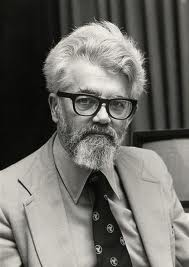
\includegraphics[width=0.8\textwidth]{chap01/10lispauthor}\\
    \tiny John McCarthy    
  \end{minipage}
  \stretchoff
\end{frame}

\begin{frame}[fragile]{发展史}{\texttt{Simula}}
  %\stretchon
  \begin{itemize}
  \item Simula
    \begin{itemize}
    \item 1967
    \item 被认为是第一个面向对象程序设计语言
    \item 第一次引入了对象、数据抽象和类的定义及继承机制
    \item 语法特点\\
      \begin{minipage}{0.8\linewidth}
        \begin{minted}[bgcolor=listinggray, gobble=8, fontsize=\tiny,
          frame=lines]{c++}
          Begin
              Class Char(c);
                  Character c;
                  Begin
                      Procedure print;
                           OutChar(c);
                  End;
          End;
        \end{minted}
      \end{minipage}
    \end{itemize}
  \end{itemize}
  \begin{center}
    \scalebox{0.5}{
      % \tikzstyle{block} = [rectangle, draw, text width=10em, text
      % centered, rounded corners, minimum height=1.0em]
      \tikzset{box/.style={rectangle, draw=black, rounded corners}}
      \tikzset{boxgreen/.style={rectangle, draw=black, rounded corners,fill=green}}
      \begin{tikzpicture}
        \node[box] (asm) {Assembler};
        \node[box] (for) [right=0.5 of asm] {Fortran};
        \node[box] (alg) [right=0.5 of for] {Algol};
        \node[box] (bcp) [right=0.5 of alg] {BCPL};
        \node[box] (pas) [above=1 of bcp] {Pascal};
        \node[boxgreen] (sim) [below=1 of bcp] {Simula};
        \node[box] (c) [right=0.5 of bcp] {C};
        \node[box] (cpp) [right=0.5 of c] {C++};
        \node[box] (cpp0x) [right=0.5 of cpp] {C++0x};
        \node[box] (opas) [above=1 of cpp0x, right=3.1 of pas] {Object Pascal};
        \node[box] (lisp) [below=2.5 of alg] {Lisp};
        \node[box] (smt) [right=2.5 of lisp] {Smalltalk};
        \node[box] (jar) [below=2.5 of cpp0x, right=0.8 of smt] {Java};
        \node (endmain) [right=0.5 of cpp0x] {};
        \node (endopas) [right=0.5 of opas] {};
        \node (endjava) [right=0.5 of jar] {};

        \draw[->] (asm) -- (for);
        \draw[->] (for) -- (alg);
        \draw[->] (alg) -- (bcp);
        \draw[->] ([xshift=0.2em]alg.east) |- (pas);
        \draw[->] ([xshift=0.2em]alg.east) |- (sim);
        \draw[->] (sim.east) -| (cpp);
        % \draw[->] (alg) -- (pas);
        \draw[->] (bcp) -- (c);
        \draw[->] (c) -- (cpp);
        \draw[->] (cpp) -- (cpp0x);
        \draw[->] (cpp0x) -- (endmain);
        \draw[->] ([xshift=0.2em]cpp.east) |- ([yshift=-0.3em]opas.west);
        \draw[->] ([xshift=0.2em]cpp.east) |- ([yshift=0.3em]jar.west);
        \draw[->] (pas) -- (opas);
        \draw[->] (opas) -- (endopas);
        \draw[->] (lisp) -- (smt);
        \draw[->] ([xshift=0.2em]sim.east) |- ([yshift=0.3em]smt.west);
        \draw[->] (smt) -- (jar);
        \draw[->] (jar) -- (endjava);
      \end{tikzpicture}
    }
    \begin{minipage}[b]{0.2\linewidth}
      \centering
      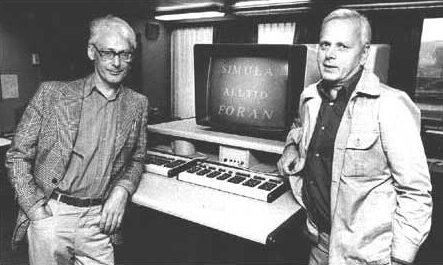
\includegraphics[width=0.8\textwidth]{chap01/11simulaauthor}\\
      \tiny Ole-Johan Dahl and Kristen Nygaard
    \end{minipage}
  \end{center}
  %\stretchoff
\end{frame}

\begin{frame}{发展史}{\texttt{Smalltalk}}
  \begin{itemize}
  \item Smalltalk
    \begin{itemize}
    \item 1972
    \item 第一个纯(Pure)面向对象程序设计语言
    \item 语法特点
      \begin{itemize}
      \item Primitives such as character and punctuation is treated as
        an object\\
        \alert{例如:3+4}\\
        Sends the message “+” to the receiver 3 with argument 4
      \end{itemize}
    \end{itemize}
  \end{itemize}
  \begin{center}
    \scalebox{0.55}{
      % \tikzstyle{block} = [rectangle, draw, text width=10em, text
      % centered, rounded corners, minimum height=1.0em]
      \tikzset{box/.style={rectangle, draw=black, rounded corners}}
      \tikzset{boxgreen/.style={rectangle, draw=black, rounded corners,fill=green}}
      \begin{tikzpicture}
        \node[box] (asm) {Assembler};
        \node[box] (for) [right=0.5 of asm] {Fortran};
        \node[box] (alg) [right=0.5 of for] {Algol};
        \node[box] (bcp) [right=0.5 of alg] {BCPL};
        \node[box] (pas) [above=1 of bcp] {Pascal};
        \node[box] (sim) [below=1 of bcp] {Simula};
        \node[box] (c) [right=0.5 of bcp] {C};
        \node[box] (cpp) [right=0.5 of c] {C++};
        \node[box] (cpp0x) [right=0.5 of cpp] {C++0x};
        \node[box] (opas) [above=1 of cpp0x, right=3.1 of pas] {Object Pascal};
        \node[box] (lisp) [below=2.5 of alg] {Lisp};
        \node[boxgreen] (smt) [right=2.5 of lisp] {Smalltalk};
        \node[box] (jar) [below=2.5 of cpp0x, right=0.8 of smt] {Java};
        \node (endmain) [right=0.5 of cpp0x] {};
        \node (endopas) [right=0.5 of opas] {};
        \node (endjava) [right=0.5 of jar] {};

        \draw[->] (asm) -- (for);
        \draw[->] (for) -- (alg);
        \draw[->] (alg) -- (bcp);
        \draw[->] ([xshift=0.2em]alg.east) |- (pas);
        \draw[->] ([xshift=0.2em]alg.east) |- (sim);
        \draw[->] (sim.east) -| (cpp);
        % \draw[->] (alg) -- (pas);
        \draw[->] (bcp) -- (c);
        \draw[->] (c) -- (cpp);
        \draw[->] (cpp) -- (cpp0x);
        \draw[->] (cpp0x) -- (endmain);
        \draw[->] ([xshift=0.2em]cpp.east) |- ([yshift=-0.3em]opas.west);
        \draw[->] ([xshift=0.2em]cpp.east) |- ([yshift=0.3em]jar.west);
        \draw[->] (pas) -- (opas);
        \draw[->] (opas) -- (endopas);
        \draw[->] (lisp) -- (smt);
        \draw[->] ([xshift=0.2em]sim.east) |- ([yshift=0.3em]smt.west);
        \draw[->] (smt) -- (jar);
        \draw[->] (jar) -- (endjava);
      \end{tikzpicture}
    }
    \begin{minipage}[b]{0.2\linewidth}
      \centering
      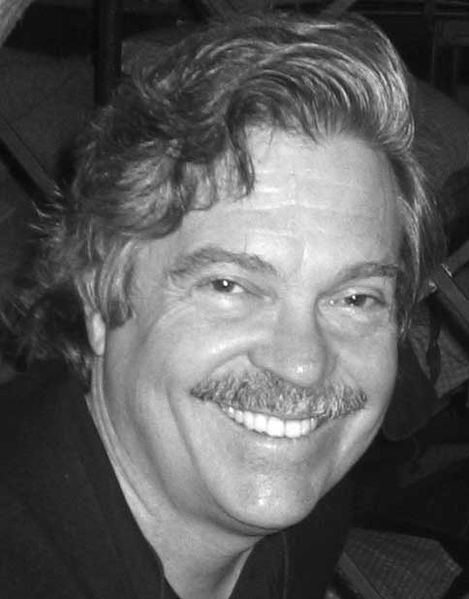
\includegraphics[width=0.8\textwidth]{chap01/12smalltalkauthor}\\
      \tiny Alan Kay
    \end{minipage}
  \end{center}
\end{frame}

\begin{frame}{发展史}{\texttt{C}}
  \begin{itemize}
  \item C
    \begin{itemize}
    \item 1972
    \item C is quirky, flawed, and an enormous success. While
      accidents of history surely helped, it evidently satisfied a
      need for a system implementation language \alert{efficient
        enough to displace assembly language}, yet \alert{sufficiently
        abstract and fluent} to describe algorithms and interactions
      in a wide variety of environments.      
    \end{itemize}
  \end{itemize}
  \begin{center}
    \scalebox{0.55}{
      % \tikzstyle{block} = [rectangle, draw, text width=10em, text
      % centered, rounded corners, minimum height=1.0em]
      \tikzset{box/.style={rectangle, draw=black, rounded corners}}
      \tikzset{boxgreen/.style={rectangle, draw=black, rounded corners,fill=green}}
      \begin{tikzpicture}
        \node[box] (asm) {Assembler};
        \node[box] (for) [right=0.5 of asm] {Fortran};
        \node[box] (alg) [right=0.5 of for] {Algol};
        \node[box] (bcp) [right=0.5 of alg] {BCPL};
        \node[box] (pas) [above=1 of bcp] {Pascal};
        \node[box] (sim) [below=1 of bcp] {Simula};
        \node[boxgreen] (c) [right=0.5 of bcp] {C};
        \node[box] (cpp) [right=0.5 of c] {C++};
        \node[box] (cpp0x) [right=0.5 of cpp] {C++0x};
        \node[box] (opas) [above=1 of cpp0x, right=3.1 of pas] {Object Pascal};
        \node[box] (lisp) [below=2.5 of alg] {Lisp};
        \node[box] (smt) [right=2.5 of lisp] {Smalltalk};
        \node[box] (jar) [below=2.5 of cpp0x, right=0.8 of smt] {Java};
        \node (endmain) [right=0.5 of cpp0x] {};
        \node (endopas) [right=0.5 of opas] {};
        \node (endjava) [right=0.5 of jar] {};

        \draw[->] (asm) -- (for);
        \draw[->] (for) -- (alg);
        \draw[->] (alg) -- (bcp);
        \draw[->] ([xshift=0.2em]alg.east) |- (pas);
        \draw[->] ([xshift=0.2em]alg.east) |- (sim);
        \draw[->] (sim.east) -| (cpp);
        % \draw[->] (alg) -- (pas);
        \draw[->] (bcp) -- (c);
        \draw[->] (c) -- (cpp);
        \draw[->] (cpp) -- (cpp0x);
        \draw[->] (cpp0x) -- (endmain);
        \draw[->] ([xshift=0.2em]cpp.east) |- ([yshift=-0.3em]opas.west);
        \draw[->] ([xshift=0.2em]cpp.east) |- ([yshift=0.3em]jar.west);
        \draw[->] (pas) -- (opas);
        \draw[->] (opas) -- (endopas);
        \draw[->] (lisp) -- (smt);
        \draw[->] ([xshift=0.2em]sim.east) |- ([yshift=0.3em]smt.west);
        \draw[->] (smt) -- (jar);
        \draw[->] (jar) -- (endjava);
      \end{tikzpicture}
    }
    \begin{minipage}[b]{0.2\linewidth}
      \centering
      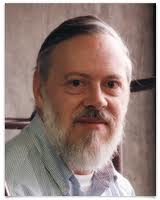
\includegraphics[width=0.8\textwidth]{chap01/13cauthor}\\
      \tiny Dennis Ritchie
    \end{minipage}
  \end{center}
\end{frame}

\begin{frame}{发展史}{\texttt{C++}}
  \begin{itemize}
  \item C++
    \begin{itemize}
    \item 1985 
    \end{itemize}
  \end{itemize}
  \begin{center}
    \scalebox{0.65}{
      % \tikzstyle{block} = [rectangle, draw, text width=10em, text
      % centered, rounded corners, minimum height=1.0em]
      \tikzset{box/.style={rectangle, draw=black, rounded corners}}
      \tikzset{boxgreen/.style={rectangle, draw=black, rounded corners,fill=green}}
      \begin{tikzpicture}
        \node[box] (asm) {Assembler};
        \node[box] (for) [right=0.5 of asm] {Fortran};
        \node[box] (alg) [right=0.5 of for] {Algol};
        \node[box] (bcp) [right=0.5 of alg] {BCPL};
        \node[box] (pas) [above=1 of bcp] {Pascal};
        \node[box] (sim) [below=1 of bcp] {Simula};
        \node[box] (c) [right=0.5 of bcp] {C};
        \node[boxgreen] (cpp) [right=0.5 of c] {C++};
        \node[box] (cpp0x) [right=0.5 of cpp] {C++0x};
        \node[box] (opas) [above=1 of cpp0x, right=3.1 of pas] {Object Pascal};
        \node[box] (lisp) [below=2.5 of alg] {Lisp};
        \node[box] (smt) [right=2.5 of lisp] {Smalltalk};
        \node[box] (jar) [below=2.5 of cpp0x, right=0.8 of smt] {Java};
        \node (endmain) [right=0.5 of cpp0x] {};
        \node (endopas) [right=0.5 of opas] {};
        \node (endjava) [right=0.5 of jar] {};

        \draw[->] (asm) -- (for);
        \draw[->] (for) -- (alg);
        \draw[->] (alg) -- (bcp);
        \draw[->] ([xshift=0.2em]alg.east) |- (pas);
        \draw[->] ([xshift=0.2em]alg.east) |- (sim);
        \draw[->] (sim.east) -| (cpp);
        % \draw[->] (alg) -- (pas);
        \draw[->] (bcp) -- (c);
        \draw[->] (c) -- (cpp);
        \draw[->] (cpp) -- (cpp0x);
        \draw[->] (cpp0x) -- (endmain);
        \draw[->] ([xshift=0.2em]cpp.east) |- ([yshift=-0.3em]opas.west);
        \draw[->] ([xshift=0.2em]cpp.east) |- ([yshift=0.3em]jar.west);
        \draw[->] (pas) -- (opas);
        \draw[->] (opas) -- (endopas);
        \draw[->] (lisp) -- (smt);
        \draw[->] ([xshift=0.2em]sim.east) |- ([yshift=0.3em]smt.west);
        \draw[->] (smt) -- (jar);
        \draw[->] (jar) -- (endjava);
      \end{tikzpicture}
    }
    \begin{minipage}[b]{0.2\linewidth}
      \centering
      
\includegraphics[width=1.0\textwidth]{chap01/14cppauthor}\\
      \tiny Bjarne Stroustrup \\ (本贾尼·斯特劳斯特卢普)
    \end{minipage}
  \end{center}
\end{frame}

\begin{frame}{发展史}{\texttt{JAVA}}
  \begin{itemize}
  \item JAVA
    \begin{itemize}
    \item 1995 
    \end{itemize}
  \end{itemize}
  \begin{center}
    \scalebox{0.7}{
      % \tikzstyle{block} = [rectangle, draw, text width=10em, text
      % centered, rounded corners, minimum height=1.0em]
      \tikzset{box/.style={rectangle, draw=black, rounded corners}}
      \tikzset{boxgreen/.style={rectangle, draw=black, rounded corners,fill=green}}
      \begin{tikzpicture}
        \node[box] (asm) {Assembler};
        \node[box] (for) [right=0.5 of asm] {Fortran};
        \node[box] (alg) [right=0.5 of for] {Algol};
        \node[box] (bcp) [right=0.5 of alg] {BCPL};
        \node[box] (pas) [above=1 of bcp] {Pascal};
        \node[box] (sim) [below=1 of bcp] {Simula};
        \node[box] (c) [right=0.5 of bcp] {C};
        \node[box] (cpp) [right=0.5 of c] {C++};
        \node[box] (cpp0x) [right=0.5 of cpp] {C++0x};
        \node[box] (opas) [above=1 of cpp0x, right=3.1 of pas] {Object Pascal};
        \node[box] (lisp) [below=2.5 of alg] {Lisp};
        \node[box] (smt) [right=2.5 of lisp] {Smalltalk};
        \node[boxgreen] (jar) [below=2.5 of cpp0x, right=0.8 of smt] {Java};
        \node (endmain) [right=0.5 of cpp0x] {};
        \node (endopas) [right=0.5 of opas] {};
        \node (endjava) [right=0.5 of jar] {};

        \draw[->] (asm) -- (for);
        \draw[->] (for) -- (alg);
        \draw[->] (alg) -- (bcp);
        \draw[->] ([xshift=0.2em]alg.east) |- (pas);
        \draw[->] ([xshift=0.2em]alg.east) |- (sim);
        \draw[->] (sim.east) -| (cpp);
        % \draw[->] (alg) -- (pas);
        \draw[->] (bcp) -- (c);
        \draw[->] (c) -- (cpp);
        \draw[->] (cpp) -- (cpp0x);
        \draw[->] (cpp0x) -- (endmain);
        \draw[->] ([xshift=0.2em]cpp.east) |- ([yshift=-0.3em]opas.west);
        \draw[->] ([xshift=0.2em]cpp.east) |- ([yshift=0.3em]jar.west);
        \draw[->] (pas) -- (opas);
        \draw[->] (opas) -- (endopas);
        \draw[->] (lisp) -- (smt);
        \draw[->] ([xshift=0.2em]sim.east) |- ([yshift=0.3em]smt.west);
        \draw[->] (smt) -- (jar);
        \draw[->] (jar) -- (endjava);
      \end{tikzpicture}
    }
    \begin{minipage}[b]{0.2\linewidth}
      \centering
      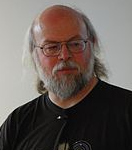
\includegraphics[width=0.8\textwidth]{chap01/15javaauthor}\\
      \tiny James Gosling
    \end{minipage}
  \end{center}
\end{frame}

%%%%%%%%%%%%%%%%%%%%%%%%%%%%%%%%%%%%%%%%%%%%%%%%%%%%%%%%%%%%%%%%%%%%%%%%%%

\section[目的]{为何使用C++实践面向对象程序设计}\label{sec:chap01-sec05}

%%%%%%%%%%%%%%%%%%%%%%%%%% 为何使用C++实践面向对象程序设计 %%%%%%%%%%%%%%%%%%%%%%%%%%%%%
\begin{frame}{目的}{面向对象程序设计}
  \stretchon
  \begin{itemize}
  \item Java\\
    网络计算(Network computing)
  \item C++\\
    系统程序设计(Systems programming)\\
    \begin{center}
      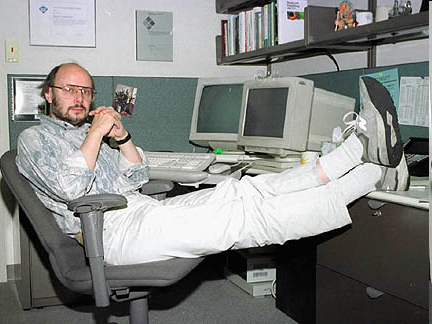
\includegraphics[width=0.4\textwidth]{chap01/16cppauthor2}\\
      \tiny Bjarne Stroustrup\\
      \url{http://www2.research.att.com/~bs/}
    \end{center}    
  \end{itemize}
  \stretchoff
\end{frame}

\begin{frame}{目的}{C++应用程序开发案例}
  \stretchon
  \begin{itemize}
  \item Adobe系统:Photoshop, Illustrator等
  \item Alias|Wavefront: Maya, Autodesk等
  \item Apple OS X重要的部分
  \item 游戏: 星际争霸,暗黑破坏神,魔兽争霸等
  \item Telecommunications
  \item Google(网络搜索引擎等)
  \item Microsoft applications and GUIs
  \item Linux tools and GUIs
  \item Amazon.com: 大型电子商务应用软件
  \item \ldots\ldots
  \end{itemize}
  \stretchoff
\end{frame}

\begin{frame}{目的}{为后续课程做准备}
  \stretchon
  \begin{itemize}
  \item Java 、C\#和Objective C
  \item 计算机图形学及计算机动画
  \item 图形图像处理
  \item 虚拟现实技术
  \item \ldots\ldots
  \end{itemize}
  \stretchoff
\end{frame}
%%%%%%%%%%%%%%%%%%%%%%%%%%%%%%%%%%%%%%%%%%%%%%%%%%%%%%%%%%%%%%%%%%%%%%%%%%

\section[程序结构]{C++程序结构}\label{sec:chap01-sec06}
%%%%%%%%%%%%%%%%%%%%%%%%%%%%%%%% C++程序结构 %%%%%%%%%%%%%%%%%%%%%%%%%%%%%%%%%%
\begin{frame}{程序结构}{C++程序结构}
  \stretchon
  \begin{itemize}
  \item 开发流程
  \end{itemize}
  % \scalebox{0.7}{
  \centering
  %\begin{center}
    \scalebox{0.95}{
    $%
    \psset{shadowcolor=black!70,shadowangle=-90,blur,shortput=nab}
    \begin{psmatrix}[rowsep=0.5,colsep=1.7]
      \psframebox[fillstyle=solid,
      fillcolor=green!30,shadow=true]{\text{编译器}} &
      \psframebox[fillstyle=solid, fillcolor=gray!30,shadow=true]{
        \begin{minipage}[c]{0.25\linewidth}
          \text{源程序.cpp}\\
          \text{头文件.h}\\
          \textcolor{red}{系统头文件}
        \end{minipage}
      }\\
      \psframebox[fillstyle=solid,
      fillcolor=yellow!30,shadow=true]{\text{预处理器}} &
      \psframebox[fillstyle=solid,
      fillcolor=gray!30,shadow=true]{\text{源程序.cpp}}\\
      \psframebox[fillstyle=solid,
      fillcolor=yellow!30,shadow=true]{\text{编译器}} &
      \psframebox[fillstyle=solid, fillcolor=gray!30,shadow=true]{
        \begin{minipage}[c]{0.25\linewidth}
          \text{目标程序.obj}\\
          \text{库文件.lib}
        \end{minipage}
      }
      & \psframebox[fillstyle=solid, fillcolor=red!30,shadow=true]{\text{调试器}} \\
      \psframebox[shadow=true]{\text{连接器}} &
      \psframebox[fillstyle=solid,
      fillcolor=gray!30,shadow=true]{\text{可执行文件.exe}}\\
      \psframebox[fillstyle=solid,
      fillcolor=red!30,shadow=true]{\text{CPU}} &
      \psframebox[shadow=true]{\text{内存}}
      \psset{arrows=->,nodesep=3pt}
      \everypsbox{\scriptstyle}
      \ncline{1,1}{2,1}
      \ncline{2,1}{3,1}
      \ncline{3,1}{4,1}
      \ncline{4,1}{5,1}
      \ncline{<->}{1,1}{1,2}^{\text{\textcolor{red}{编辑}}}
      \ncline{1,2}{2,1}
      \ncline{2,1}{2,2}^{\text{\textcolor{red}{预处理}}}
      \ncline{2,2}{3,1}
      \ncline{3,1}{3,2}^{\text{\textcolor{red}{编译}}}
      \ncline{3,2}{4,1}
      \ncline{4,1}{4,2}^{\text{\textcolor{red}{连接}}}
      \ncline{4,2}{5,2}>{\text{\textcolor{red}{载入}}}
      \ncline{5,1}{5,2}^{\text{\textcolor{red}{运行}}}
      \ncangle[angleA=90,angleB=0, armB=0, linearc=0]{3,3}{1,2}>{\text{\textcolor{red}{调试}}}
      \ncangle[angleA=-90,angleB=0, armB=0, linearc=0]{3,3}{5,2}>{\text{\textcolor{red}{调试}}}
    \end{psmatrix}
    $%
    }
    % \end{center}
  \stretchoff  
\end{frame}

\begin{frame}{程序结构}{集成开发环境---IDE}
  \stretchon
  \begin{itemize}
  \item 辅助程序
  \item 工具
    \begin{itemize}
    \item 编辑器
    \item 编译器/解释器
    \item 自动建立工具
    \item 调试器
    \item 版本控制器
    \item GUI设计器
    \item \ldots\ldots
    \end{itemize}
  \end{itemize}
  \stretchoff
\end{frame}

\begin{frame}{程序结构}{IDE---DEV C++}
  \stretchon
  \begin{itemize}
  \item DEV C++
  \end{itemize}
  \centering
  %\begin{center}
    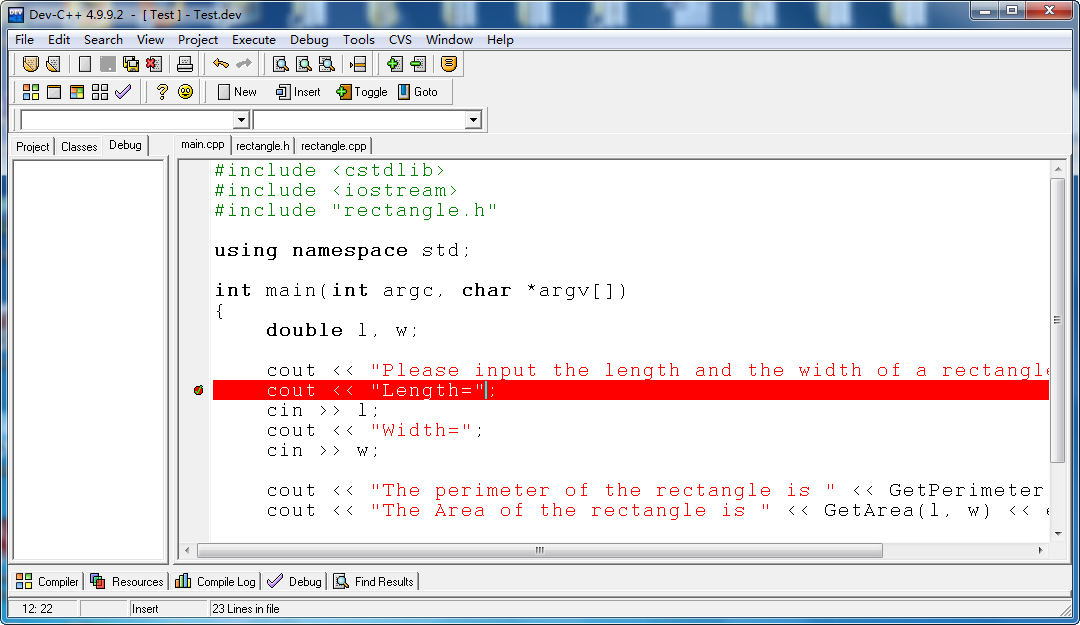
\includegraphics[height=0.6\textheight]{chap01/17idedevc}\\
    \tiny
    \url{http://sourceforge.net/projects/orwelldevcpp/}
    % \end{center}
  \stretchoff
\end{frame}

\begin{frame}{程序结构}{IDE---Visual Studio 2005}
  \stretchon
  \begin{itemize}
  \item Visual Studio 2005
  \end{itemize}
  \centering
  %\begin{center}
    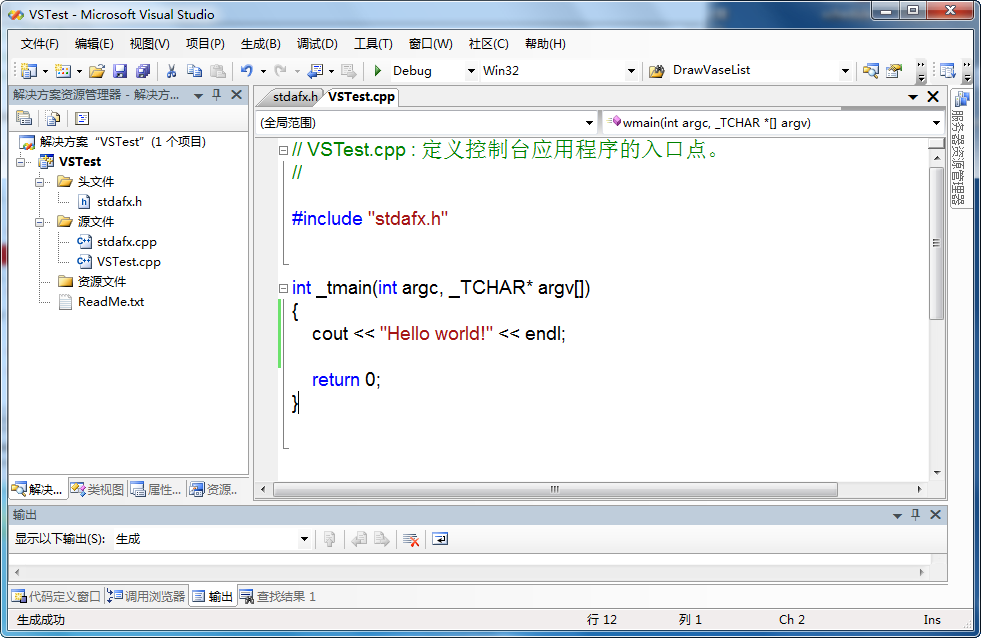
\includegraphics[height=0.6\textheight]{chap01/18idevs2005}\\
    \tiny
    \url{http://www.visualstudio.com/}
  %\end{center}
  \stretchoff
\end{frame}

\begin{frame}{程序结构}{IDE---Code::Blocks}
  \stretchon
  \begin{itemize}
  \item Code::Blocks
  \end{itemize}
  \centering
  %\begin{center}
    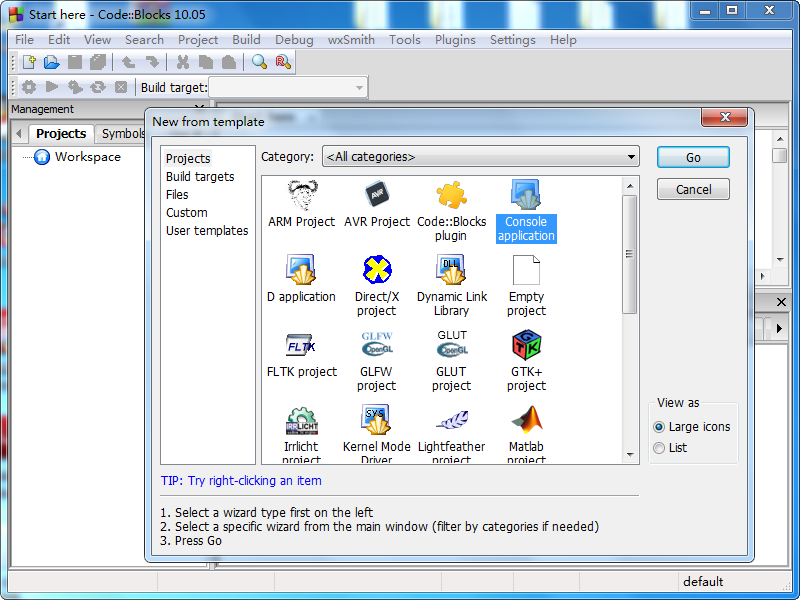
\includegraphics[height=0.6\textheight]{chap01/19idecb}\\
    \tiny
    \url{http://www.codeblocks.org/}
  %\end{center}
  \stretchoff
\end{frame}

\begin{frame}{程序结构}{IDE---QT}
  \stretchon
  \begin{itemize}
  \item QT
  \end{itemize}
  \centering
  %\begin{center}
    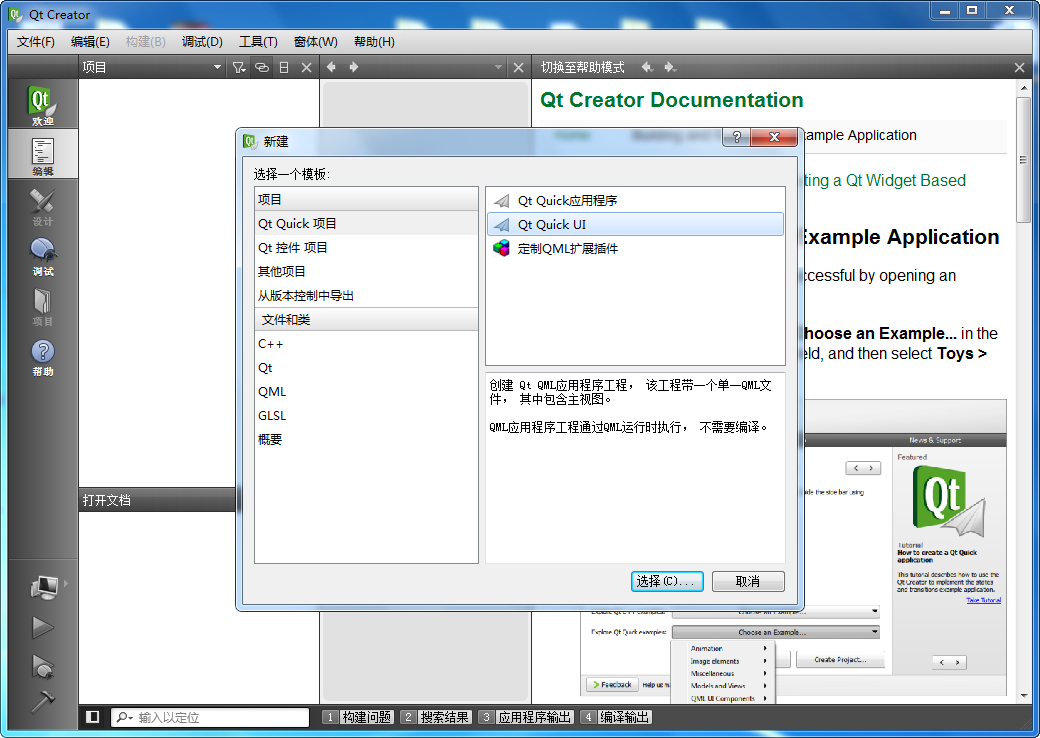
\includegraphics[height=0.6\textheight]{chap01/20ideqt}\\
    \tiny
    \url{http://qt-project.org/}
  %\end{center}
  \stretchoff
\end{frame}
  
  
%%%%%%%%%%%%%%%%%%%%%%%%%%%%%%%%%%%%%%%%%%%%%%%%%%%%%%%%%%%%%%%%%%%%%%%%%%


\section[基本程序]{基本C++程序}\label{sec:chap01-sec07}
%%%%%%%%%%%%%%%%%%%%%%%%%%%%%%%% 基本C++程序 %%%%%%%%%%%%%%%%%%%%%%%%%%%%%%%%%%
\begin{frame}[fragile]{基本程序}{基本C++程序}
  \vspace{-2ex}
  \begin{center}
    \begin{minipage}{0.8\linewidth}
      \cppfile{codes/chap01/ex01-01.cpp}
    \end{minipage}
  \end{center}
  \vspace{-4ex}
  \begin{itemize}
  \item 名字空间 (namespace)\\
    \begin{minipage}{0.8\linewidth}
      \begin{cppcode}
using namespace std;
      \end{cppcode}
    \end{minipage}
  \item 输入/输出
    \begin{itemize}
    \item cin对象\\
      \begin{minipage}{0.8\linewidth}
      \begin{cpptt}
cin >> |对象1| >> |对象2| >> |$\cdots$| >> |对象n|;
      \end{cpptt}
    \end{minipage}
  \item cout对象\\
    \begin{minipage}{0.8\linewidth}
      \begin{cpptt}
cout << |对象1| << |对象2| << |$\cdots$| << |对象n|;
      \end{cpptt}
    \end{minipage}
    \end{itemize}
  \end{itemize}
\end{frame}

\begin{frame}[fragile]{基本程序}{基本C++程序}%label=testframe,
  %\begin{spacing}{1.2}
  \begin{itemize}
  \item 两个整数的加法       
  \end{itemize}
  \begin{center}
    \begin{tikzpicture}[font=\scriptsize]
      % 绘制代码
      \umlnote[scale=0.95, text width=0.65\textwidth](code1) at (0, 0)
      {
        \cppfile{codes/chap01/ex01-02.cpp}
      };
    \end{tikzpicture}
  \end{center}
  %\end{spacing}
\end{frame}
%%%%%%%%%%%%%%%%%%%%%%%%%%%%%%%%%%%%%%%%%%%%%%%%%%%%%%%%%%%%%%%%%%%%%%%%%%

% 附件页
\section[附件下载]{本讲示例代码及附件下载} 
\begin{frame}[t]{附件}{本讲附件}
  % 此处的[ucfilespec=...]必须指定为pdf否则Windows下无法下载
  %\vspace{-4ex}
  \textattachfile[ucfilespec=ex-src01.pdf]{ex-src01.zip}{附件:右键单击该
    链接,选择\qtmark{\alert{保存附件}}下载,\alert{将后缀名改为\qtmark{.zip}解压}
      \footnote[frame]{请\alert{退出全屏模式}后点击该链接。}
      \footnote[frame]{以Adobe Acrobat Reader为例。}
      。}%\\

  \vspace{-1ex}
  \begin{center}
    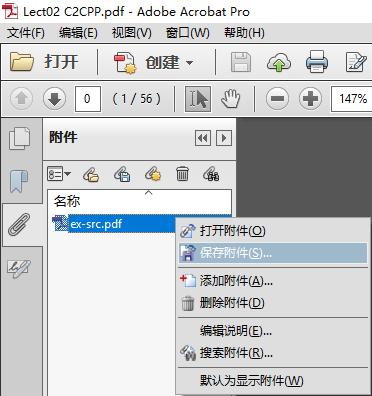
\includegraphics[height=0.35\textheight]{pdfattatchdownload01}\quad
    %或 \quad%
    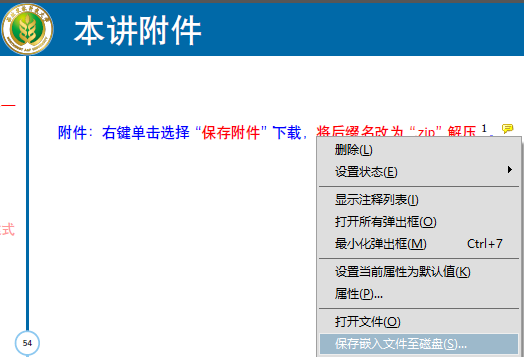
\includegraphics[height=0.35\textheight]{pdfattatchdownload02}\\[2ex]%
    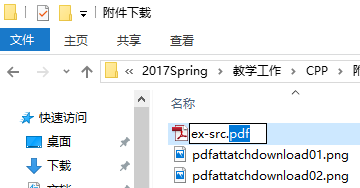
\includegraphics[height=0.255\textheight]{pdfattatchdownload03}\quad
    %$\Rightarrow$ \quad%
    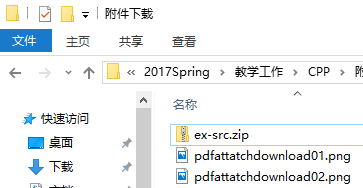
\includegraphics[height=0.255\textheight]{pdfattatchdownload04}%
  \end{center}   
\end{frame}

% \tiny
% \scriptsize
% \footnotesize
% \small
% \normalsize
% \large
% \Large
% \LARGE
% \huge
% \Huge


%%% Local Variables: 
%%% mode: latex
%%% TeX-master: "../main.tex"
%%% End: 
 % 基础知识
  \or % 第2章
    \lecture{绪论}{lec:chap02}
\section[知识回顾]{知识回顾}\label{sec:chap02-sec00}
%%%%%%%%%%%%%%%%%%%%%%%%%%%%%% 知识回顾 %%%%%%%%%%%%%%%%%%%%%%%%%%%%%%%%%%
%\stretchon%和\stretchoff
\begin{frame}[t, fragile]{知识回顾}{面向对象的基本概念}
  \stretchon
  \begin{itemize}
  \item 对象、类及其特性%\hilite<1>
    \begin{itemize}
    \item 什么是对象
    \item 什么是类
    \item 四大特性(数据抽象 、封装、继承和多态)
    \end{itemize}
  \item 面向对象程序设计语言发展史    
  \item 基本C++程序
    \begin{itemize}
    \item \cppinttfts{cin} 和 \cppinttfts{cout}
    \item \cppinttfts{using namespace}
    \end{itemize}
  \end{itemize}
  \stretchoff
\end{frame}
%\stretchoff

\begin{frame}{知识回顾}{发展史}
  \stretchon
  \begin{itemize}
  \item 族谱(Family tree)    
  \end{itemize}
  \centering
      \scalebox{0.7}{
        \centering
        %\tikzstyle{block} = [rectangle, draw, text width=10em, text centered, rounded corners, minimum height=1.0em]
        \tikzset{box/.style={rectangle, draw=black, rounded corners}}
        \tikzset{boxgreen/.style={rectangle, draw=black, rounded corners,fill=green}} 
        \begin{tikzpicture}
          \node[box] (asm) {Assembler};
          \node[box] (for) [right=0.5 of asm] {Fortran};
          \node[box] (alg)  [right=0.5  of for] {Algol};
          \node[box] (bcp)  [right=0.5  of alg] {BCPL};
          \node[box] (pas)  [above=1  of bcp] {Pascal};
          \node[box] (sim) [below=1 of bcp] {Simula};
          \node[box] (c) [right=0.5 of bcp] {C};
          \node[box] (cpp) [right=0.5 of c] {C++};
          \node[box] (cpp0x) [right=0.5 of cpp] {C++0x};
          \node[box] (opas) [above=1 of cpp0x, right=3.1 of pas] {Object Pascal};
          \node[box] (lisp) [below=2.5 of alg] {Lisp};
          \node[box] (smt) [right=2.5 of lisp] {Smalltalk};
          \node[box] (jar) [below=2.5 of cpp0x, right=0.8 of smt] {Java};
          \node (endmain)  [right=0.5  of cpp0x] {};
          \node (endopas)  [right=0.5 of opas] {};
          \node (endjava)  [right=0.5  of jar] {};

          \draw[->] (asm) -- (for);
          \draw[->] (for) -- (alg);
          \draw[->] (alg) -- (bcp);
          \draw[->] ([xshift=0.2em]alg.east) |- (pas);
          \draw[->] ([xshift=0.2em]alg.east) |- (sim);
          \draw[->] (sim.east) -|  (cpp);
          %\draw[->] (alg) -- (pas);
          \draw[->] (bcp) -- (c);
          \draw[->] (c) -- (cpp);
          \draw[->] (cpp) -- (cpp0x);
          \draw[->] (cpp0x) -- (endmain);
          \draw[->] ([xshift=0.2em]cpp.east) |-  ([yshift=-0.3em]opas.west);
          \draw[->] ([xshift=0.2em]cpp.east) |- ([yshift=0.3em]jar.west);
          \draw[->] (pas) -- (opas);
          \draw[->] (opas) -- (endopas);
          \draw[->] (lisp) -- (smt);
          \draw[->] ([xshift=0.2em]sim.east) |- ([yshift=0.3em]smt.west);
          \draw[->] (smt) -- (jar);
          \draw[->] (jar) -- (endjava);
        \end{tikzpicture}
      }
  \stretchoff
\end{frame}

\begin{frame}[fragile]{知识回顾}{基本C++程序}
  \begin{spacing}{1.1}%stretchon
  \begin{itemize}
  \item Hello, your name!\\
    \begin{center}
      \begin{minipage}{0.45\linewidth}
        \cppfile{codes/chap01/ex01-01.cpp}
      \end{minipage}
    \end{center}
  \item 名字空间
    \begin{itemize}
    \item \cppinttfts{using namespace}
    \end{itemize}
  \item 文件后缀名
    \begin{itemize}
    \item Windows: \cppinttfts{.cpp}
    \item Unix/Linux: \cppinttfts{.cpp}, \cppinttfts{.cc} or \cppinttfts{.c}
    \end{itemize}
  \end{itemize}
  \end{spacing}%stretchoff
\end{frame}
%%%%%%%%%%%%%%%%%%%%%%%%%%%%%%%%%%%%%%%%%%%%%%%%%%%%%%%%%%%%%%%%%%%%%%%%%%

\section[对C的扩充]{C++对C的扩充}\label{sec:chap02-sec01}
%%%%%%%%%%%%%%%%%%%%%%%%%%%%%% C++对C的扩充 %%%%%%%%%%%%%%%%%%%%%%%%%%%%%%%
\begin{frame}{扩充}{C++对C的扩充}
  \stretchon
  \begin{itemize}
  \item 格式化输入输出
  \item 基本数据类型与表达式
  \item 控制结构
  \item 构造数据类型
  \item 函数
  \item 大型程序结构控制
  \end{itemize}
  \stretchoff
\end{frame} 
%%%%%%%%%%%%%%%%%%%%%%%%%%%%%%%%%%%%%%%%%%%%%%%%%%%%%%%%%%%%%%%%%%%%%%%%%%

\section[输入输出]{格式化输入输出}\label{sec:chap02-sec02}
\subsection[cin/cout]{cin/cout}
%%%%%%%%%%%%%%%%%%%%%%%%%%%%% 格式化输入输出 %%%%%%%%%%%%%%%%%%%%%%%%%%%%%%
\begin{frame}[fragile]{输入输出}{格式化}%label=testframe,
  \begin{itemize}
  \item \cppinline{cin/cout}
  \end{itemize}
  \begin{center}
    \begin{tikzpicture}[show background grid]
      \tiny
      \umlnote[text width=0.55\textwidth](code1) at (0, 0)
      {
        \cppfiletikz{codes/chap02/ex02-01.cpp}
      };
    \end{tikzpicture}
    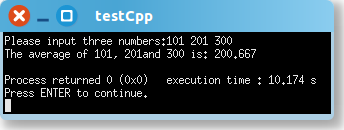
\includegraphics[width=0.45\textwidth]{chap02/01cppoutput01}
  \end{center}
\end{frame}  

\subsection[格式控制]{格式控制}
\begin{frame}[fragile]{输入输出}{输出格式设置}%
  \begin{itemize}
  \item 格式控制
  \end{itemize}
  \begin{spacing}{1.8}
  \begin{center}
    \scriptsize
    \begin{tabular}{|c|l|l|}
      \hline
      操作符 & 作用 & 说明 \\
      \hline
      \cppinttscr{oct} & 数据以8进制形式输出 & \multirow{3}{2cm}{作用范
                                              围为后续输出的整数,对小数不起作用}\\
      \cline{1-2}
      \cppinttscr{dec} & 数据以10进制形式输出(默认) & \\
      \cline{1-2}
      \cppinttscr{hex} & 数据以16进制形式输出 & \\
      \hline
      \cppinttscr{endl} & 换行并刷新输出流 & \\
      \hline
      \cppinttscr{setw(n)} & 设置输出宽度 & \multirow{2}{2cm}{作用范围为后续对象}\\
      \cline{1-2}
      \cppinttscr{setprecision(n)} & 设置输出精度(默认为6) & \\
      \hline
    \end{tabular}
    \begin{minipage}{0.65\linewidth}
      \scriptsize
      \begin{alertblock}{注意:}
        \begin{itemize}
        \item \cppinttscr{#include <iomanip>}
        \item 默认情况下, \cppinttscr{setprecision(n)}仅对带有小
          数的数有效, n为整数与小数位数之和
        \end{itemize}
      \end{alertblock}
    \end{minipage}
  \end{center}
  \end{spacing}
\end{frame}

\begin{frame}[fragile]{输入输出}{输出格式设置}%label=testframe,
  \begin{itemize}
  \item 设置输出格式
  \end{itemize}
  \begin{center}
    \begin{tikzpicture}[show background grid]
      \tiny
      \umlnote[scale=0.95, text width=0.55\textwidth](code1) at (0, 0)
      {
        \cppfiletikz{codes/chap02/ex02-02.cpp}
      };
    \end{tikzpicture}
    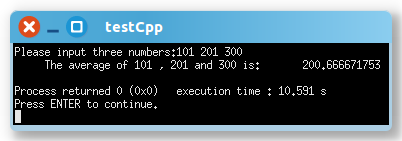
\includegraphics[width=0.45\textwidth]{chap02/01cppoutput02}
  \end{center}
\end{frame}  

  
%%%%%%%%%%%%%%%%%%%%%%%%%%%%%%%%%%%%%%%%%%%%%%%%%%%%%%%%%%%%%%%%%%%%%%%%%% 

\section[类型与表达式]{基本数据类型与表达式}\label{sec:chap02-sec03}
\subsection[基本类型]{基本类型}
\begin{frame}[t, fragile]{类型与表达式}{基本数据类型}
  \stretchon
  \begin{itemize}
  \item 基本数据类型
    \begin{itemize}
    \item \cppinttfts{int}, \cppinttfts{float}, \cppinttfts{double}, \cppinttfts{void}, \cppinttfts{char}
    \item 布尔型:\cppinttfts{bool} (\cppinttfts{true}$\Rightarrow$1, \cppinttfts{false}$\Rightarrow$0)
    \end{itemize}
  \item 变量与常量
    \begin{itemize}
    \item 变量的定义与赋初值
      \begin{itemize}
      \item \cppinttscr{int sum=100; double pi=3.1416; char c='a';}
      \item \cppinttscr{int sum(100); double pi(3.1416); char c('a');}
      \end{itemize}
    \item 符号常量与常变量
      \begin{itemize}
      \item \cppinttscr{#define PI 3.1416}
      \item \cppinttscr{const float PI=3.1416;}
      \item \cppinttscr{PI = 3.1415926535898;      // 错误!}
      \end{itemize}
    \end{itemize}
  \end{itemize}
  \stretchoff
\end{frame}

\subsection[新类型]{C++新类型}
\begin{frame}[fragile]{类型与表达式}{C++11中的新类型}
  \stretchon
  \begin{itemize}
  \item 常量表达式\\
  %\begin{center}
    \begin{minipage}{0.85\linewidth}
      \begin{cppcode}
const int size = 20;          // size是常量表达式
const int limits = size + 1;  // limits是常量表达式
int max = 80;                 // max不是常量表达式,80是字面值常量,
                              // 但max不是const, 不保证运行是不变。
const int lines = get_size(); // lines不是常量表达式
                              // lines是常量,但get_size()运行时才能确定
      \end{cppcode}
    \end{minipage}
  %\end{center}
  \item  \cppinline{constexpr}类型(验证是不是常量表达式)\\
     \begin{minipage}{0.85\linewidth}
      \begin{cppcode}
constexpr int size = 20;           // 20是常量表达式
constexpr int limits = size + 10;  // size + 10是常量表达式
constexpr int max = length();      // 取决于length()函数是不是常量函数
      \end{cppcode}
    \end{minipage}
  \item \cppinline{constexpr}与\cppinline{const}\\
    \begin{minipage}{0.85\linewidth}
      \begin{cppcode}
constexpr int a = length(); // 必须在编译时能计算出length()返回值
const int b = length();     // b的值可以在运行时获得,之后不再改变
      \end{cppcode}
    \end{minipage}
  \end{itemize}
  \stretchoff
\end{frame}

\begin{frame}[fragile]{类型与表达式}{C++11中的新类型}
  \stretchon
  \begin{itemize}
  \item \cppinline{auto}类型说明符\\
  %\begin{center}
    \begin{minipage}{0.95\linewidth}
      \begin{cppcode}
auto x = 5;               // 5是int类型,x则是int类型
auto size = sizeof(int);  // size是表示内存字节数的类型
auto name = "world";      // name是保存字符串的类型
cout << "hello " << name; // 可以使用name
auto a;                   // 错误!没有初始值无法确定类型
auto r = 1, pi = 3.14;    // 错误!类型混淆
     \end{cppcode}
    \end{minipage}
  %\end{center}
  \item  \cppinline{decltype}类型指示符,\alert{返回操作数类型}\\
     \begin{minipage}{0.95\linewidth}
      \begin{cppcode}
decltype(sizeof(int)) size; // sizeof(int)结果的类型
const int ci = 0;           // 是常量表达式
decltype(ci) x = 1;         // const int 类型
decltype(f()) y = sum;      // 函数f()的返回值类型
      \end{cppcode}
    \end{minipage}
  \end{itemize}
  \stretchoff
\end{frame}

\subsection[运算符与表达式]{运算符与表达式}
\begin{frame}[fragile]{类型与表达式}{运算符与表达式}
  \begin{spacing}{1.3}
  \begin{itemize}
  \item 运算符与表达式
    \begin{itemize}
    \item 算术运算符:\cppinttfts{+(|正号|), -(|负号|), *, /, %(|取余|)}
    \item 关系运算符:\cppinttfts{>, <, >=, <=, ==, !=}
    \item 逻辑运算符:\cppinttfts[escapeinside=//]{!, &&, ||}
    \item 位运算符: \cppinttfts[escapeinside=//]{~, <<, >>, &, ^(/异或/), /|/}
    \item 赋值运算符:\cppinttfts{=, *=, /=, %=, +=, -=, |$\cdots$|}
    \item 递增递减运算符:\cppinttfts{++, --}
    \end{itemize}
  \end{itemize}
  \centering  
  \begin{minipage}{0.3\linewidth}
    \scriptsize
    \begin{gather*}
      ax^{2}+bx+c=0 \\
      x_{1,2}=\frac{-b \pm \sqrt{b^{2}-4ac}}{2a}
    \end{gather*}
  \end{minipage}\\
  \begin{minipage}{0.6\linewidth}
    \begin{cppcode}
if(abs(b * b - 4 * a * c) > 1.0e - 10)
{
    x1 = (-b + sqrt(b * b - 4 * a * c)) / (2 * a);
    x2 = (-b - sqrt(b * b - 4 * a * c)) / (2 * a);
}
    \end{cppcode}
  \end{minipage}
  
  \end{spacing}
\end{frame}
%%%%%%%%%%%%%%%%%%%%%%%%%%%%%%%%%%%%%%%%%%%%%%%%%%%%%%%%%%%%%%%%%%%%%%%%%%

\section[控制结构]{控制结构}\label{sec:chap02-sec04}
%%%%%%%%%%%%%%%%%%%%%%%%%% 控制结构 %%%%%%%%%%%%%%%%%%%%%%%%%%%%%
\subsection[基本结构]{基本结构}
\begin{frame}[t, fragile]{控制结构}{基本结构}
  \stretchon
  \begin{itemize}
  \item 判断
    \begin{itemize}
    \item \cppinttfts{if ... else ...}
    \item \cppinttfts{if ... else if ... else ...}
    \item \cppinttfts{switch ... case ...}
    \end{itemize}
  \item 循环
    \begin{itemize}
    \item \cppinttfts{for(exp1;exp2;exp3){...}}
    \item \cppinttfts{while(exp){...}}
    \item \cppinttfts{do ... while(exp);}
    \end{itemize}
  \item 转移
    \begin{itemize}
    \item \cppinttfts{break}
    \item \cppinttfts{continue}
    \item \cppinttfts{goto}
    \end{itemize}
  \end{itemize}
  \stretchoff
\end{frame}

\subsection[范围for语句]{范围for语句}
\begin{frame}[fragile]{控制结构}{C++11中的范围for语句}
  \stretchon
  \begin{itemize}
  \item 范围\cppinline{for}语句\\[-1ex]
  %\begin{center}
    \begin{minipage}{0.95\linewidth}
      \begin{cppcode}
for(declaration : expression){
  statement;
}
// 其中:
//   expression必须是一个序列(列表、数组、vector、string等),
//     能返回begin和end对象。
//   declaration是一个变量,序列中每个元素都能够转换为该类型,
//     常用auto声明
      \end{cppcode}
    \end{minipage}
  %\end{center}
  \item 范围\cppinline{for}示例\\[-1ex]
     \begin{minipage}{0.95\linewidth}
      \begin{cppcode}
// 累加20以内的素数
int sum = 0;
for(int e : {2, 3, 5, 7, 11, 13, 17, 19}) // 用auto类型更合理
    sum += e;
cout << sum << endl;                      // 输出结果77
int arr[] = {1, 3, 5, 7, 9};              // 声明数组arr,初始化为5个奇数
for(auto ele : arr){                      // 声明ele,与数组arr关联在一起,用了auto
  ele = ele * 2;                          // 修改数组每个元素的值
  cout << ele << " ";                     // 输出ele,2 6 10 14 18
}
cout << endl;
for(auto ele : arr)
    cout << ele << " ";                   // 没有改变:1 3 5 7 9
cout << endl;
      \end{cppcode}
    \end{minipage}
  \end{itemize}
  \stretchoff
\end{frame}
%%%%%%%%%%%%%%%%%%%%%%%%%%%%%%%%%%%%%%%%%%%%%%%%%%%%%%%%%%%%%%%%%%%%%%%%%% 

\section[复杂类型]{复杂数据类型}\label{sec:chap02-sec05}
%%%%%%%%%%%%%%%%%%%%%%%%%%%%%%%% 构造数据类型 %%%%%%%%%%%%%%%%%%%%%%%%%%%%%%%%%%
% \begin{frame}[t, fragile]{复杂类型}{枚举和数组}
%   \stretchon
%   \begin{itemize}
%   \item 枚举类型
%     \begin{itemize}%\mintinline{c++}{}
%     \item \cppinline{enum weekday{SUN, MON,...,SAT};}
%     \end{itemize}
%   \item 数组
%     \begin{itemize}
%     \item 一维数组定义与初始化\\
%       \cppinline{int a[4]={1,2,3,4}; }\\
%       \cppinline{int a[]={1,2,3,4};}\\
%       \cppinline{char str[256]="movie.rm";}\\
%       \cppinline{char str[] = "movie.rm";}
%     \item 二维数组定义与初始化\\
%       \cppinline{int a[3][3]={{1,2,3},{4,5,6},{7,8,9}};}\\
%       \cppinline{int a[][3]={{1,2,3},{4,5,6},{7,8,9}};}
%     \end{itemize}  
%   \end{itemize}
%   \stretchoff
% \end{frame}
\subsection[指针与内存]{指针与内存}
\begin{frame}[t, fragile]{复杂类型}{指针}
  \begin{itemize}  
  \item 指针    
  \end{itemize}
  \hfill
  \begin{minipage}{0.35\linewidth}
    \begin{cppcode}    
int a=255;
int *p;
p=&a;
    \end{cppcode}
  \end{minipage}
  \begin{minipage}{0.6\linewidth}
    \tiny
    \begin{bytefield}{24}
      \begin{rightwordgroup}{\&a}
        \memsection[\&p$\rightarrow$]{0x00ff ffee}{0x00ff fffb}{4}{00FF 4212}
      \end{rightwordgroup}\\
      \memsection{}{}{4}{\ldots\ldots}\\
      \begin{rightwordgroup}{a}
        \memsection[\&a$\to$]{0x00ff 4212}{0x00ff 420f}{4}{0000 00FF}
      \end{rightwordgroup}\\
    \end{bytefield}
  \end{minipage}\\
  \begin{center}
    \begin{minipage}{0.7\linewidth}
      \begin{cppcode}      
float x[5];
float *p = x;
double sum = 0.0;
for (int i = 0; i < 5; i++)
{
  sum += *p++;
}      
      \end{cppcode}
    \end{minipage}
  \end{center}
\end{frame}

%\subsection[动态内存分配]{动态内存分配}
\begin{frame}[fragile]{复杂类型}{动态内存分配}
  \begin{itemize}
  \item 动态内存分配    
    \begin{itemize}
    \item \cppinttfts{malloc}和\cppinttfts{free}
    \item \cppinttfts{new}和\cppinttfts{delete}
    \end{itemize}  
  \end{itemize}
  \begin{center}
    \begin{minipage}{0.55\linewidth}
      \begin{cppcode}
// C语言
float *x = (float *)malloc(n*sizeof(float));
free (x);

// C++语言
float *x = new float[n];
delete []x;
      \end{cppcode}
    \end{minipage}\\%qquad
    \begin{minipage}{0.35\linewidth}
      \begin{cppcode}
int **mat;
int m, n;
mat = new int *[m];

for (i = 0; i < m; i++)
    mat[i] = new int[n];

for (i = 0; i < m; i++)
    delete [] mat[i];
delete [] mat;
      \end{cppcode}
    \end{minipage}
  \end{center}
\end{frame}
%\subsection[定位new表达式]{定位new表达式}
\begin{frame}[fragile]{复杂类型}{动态内存分配}
  \begin{itemize}
  \item 定位\cppinline{new}表达式
    \begin{itemize}
    \item 语法:\cppinttfts{new (|指针|)|类型|}
    \end{itemize}  
  \end{itemize}
  \begin{center}
    \begin{minipage}{0.7\linewidth}
      \begin{cppcode}
#include <iostream>
#include <new> // 必须包含该头文件

using namespace std;

char * buf = new char[1000]; // 预分配空间        

int main()
{
    int * pi = new (buf) int; // 在buf中创建一个int对象

    return 0;
}
      \end{cppcode}
    \end{minipage}
  \end{center}
\end{frame}

\subsection[指针与常量]{指针与常量}
\begin{frame}[t,fragile]{复杂类型}{指针常量和常量指针}
  \begin{itemize}
  \item 指针常量\\
    \begin{center}
      \begin{minipage}{0.6\linewidth}
        \begin{cppcode}
int a = 2, b = 3;
int * const p = &a;  //定义时必须赋初值
p = &b;              //错误,地址不能被修改
*p = b;              //正确,内容可以被修改
        \end{cppcode}
      \end{minipage}
    \end{center}
  \item 常量指针\\
    \begin{center}
      \begin{minipage}{0.55\linewidth}
        \begin{cppcode}
int a = 2, b = 3;
const int * p; 
p = &b;         //正确,地址可以被修改
*p = b;         //错误,内容不可以被修改
        \end{cppcode}
      \end{minipage}
    \end{center}
  \item 常指针常量\\
    \begin{center}
      \begin{minipage}{0.65\linewidth}
        \begin{cppcode}
int a = 2, b = 3;
const int * const p = &a;  //定义时必须赋初值
p = &b;         //错误,地址不能被修改
*p = b;         //错误,内容不可以被修改
        \end{cppcode}
      \end{minipage}
    \end{center}
  \end{itemize}
\end{frame}
\subsection[引用类型]{引用类型}
\begin{frame}[t, fragile]{复杂类型}{引用类型}
  \begin{itemize}
  \item 引用是已存在的变量的别名\\
    \begin{center}
      \begin{minipage}{0.6\linewidth}
        \begin{cppcode}
int i = 3;
int &j = i;   //引用必须赋初值
int &j = 3;   //错误,初值必须为变量
j = 4;
        \end{cppcode}
      \end{minipage}
    \end{center}
  \item 引用和指针的区别与联系\\
    \begin{center}
      \begin{minipage}{0.45\linewidth}
        \begin{cppcode}
int i = 3;
int &j = i;
int *k = &i;
cout << &i << endl;
cout << &j << endl;
cout << &k << endl;
        \end{cppcode}
      \end{minipage}
      \begin{minipage}{0.5\linewidth}
        \tiny
        \begin{bytefield}{24}
          \memsection{$\cdots$}{}{1}{$\cdots$}\\
          \memsection[k$\rightarrow$]{0x0016 FDEC}{}{1}{0x0016 FE04}\\
          \memsection{$\cdots$}{}{1}{$\cdots$}\\
          \memsection[$\genfrac{}{}{0pt}{}{\texttt{i}}{\texttt{j}}\rightarrow$]{0x0016 FE04}{}{1}{0x0000 0003}\\
          \memsection{$\cdots$}{}{1}{$\cdots$}
        \end{bytefield}
      \end{minipage}
    \end{center}
  \end{itemize}
\end{frame}

\begin{frame}[t, fragile]{复杂类型}{引用类型}
  \begin{itemize}
  \item 引用作为函数参数(例1)\\[-0.5ex]
    \begin{center}
      \scalebox{0.8}{
        \begin{minipage}{0.5\linewidth}
          \cppfile[fontsize=\scriptsize]{codes/chap02/ex02-03.cpp}
        \end{minipage}\qquad\qquad
        \begin{minipage}{0.5\linewidth}
          \cppfile[fontsize=\scriptsize]{codes/chap02/ex02-04.cpp}
        \end{minipage}
      }
    \end{center}
  \end{itemize}
\end{frame}

% \begin{frame}[t, label=testframe, fragile]{输出格式设置}%label=testframe,
%   \begin{center}
%     \begin{tikzpicture}[show background grid]
%       \tiny
%       \umlnote[text width=0.75\textwidth](code1) at (0, 0)
%       {
%         \cppfiletikz{codes/chap02/ex02-02.cpp}
%       };
%     \end{tikzpicture}
%     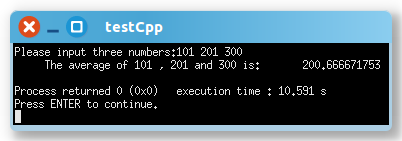
\includegraphics[width=0.5\textwidth]{chap02/01cppoutput02}
%   \end{center}
% \end{frame} 


\begin{frame}[t, fragile]{复杂类型}{引用类型}
  \begin{itemize}
  \item 引用作为函数参数(例2)\\
    \begin{center}
      \begin{minipage}{0.35\linewidth}
        \begin{cppcode}
struct StuNode
{
    int ID;
    char name[128];
    bool gender;
    int age;
    struct StuNode *next;
};
        \end{cppcode}
      \end{minipage}\qquad
      \begin{minipage}{0.5\linewidth}
        \begin{tikzpicture}[show background grid]
          \tiny
          \umlnote[text width = 0.85\textwidth](code1) at (0, 0)
          {
            \cppfiletikz{codes/chap02/ex02-05.cpp}
          };          
        \end{tikzpicture}        
        %\cppfile{codes/chap02/ex02-05.cpp}
      \end{minipage}
    \end{center}
  \end{itemize}
\end{frame}

\begin{frame}[t, fragile]{复杂类型}{引用类型}
  \begin{itemize}
  \item 引用作为函数参数(例2)\\
    \begin{center}
      \begin{minipage}{0.35\linewidth}
        \begin{cppcode}
struct StuNode
{
  int ID;
  char name[128];
  bool gender;
  int age;
  struct StuNode *next;
};
        \end{cppcode}
      \end{minipage}\qquad
      \begin{minipage}{0.5\linewidth}
        \begin{tikzpicture}[show background grid]
          \tiny
          \umlnote[text width = 0.85\textwidth](code1) at (0, 0)
          {
            \cppfiletikz{codes/chap02/ex02-06.cpp}
          };          
        \end{tikzpicture}
        %\cppfile{codes/chap02/ex02-06.cpp}
      \end{minipage}
    \end{center}
  \end{itemize}
\end{frame}

\begin{frame}[t,fragile]{复杂类型}{引用类型}
  \begin{itemize}
  \item 常引用\\
    \begin{minipage}{0.8\linewidth}
      \begin{cppcode}
int i = 100;
const int &r1 = 100;            //正确
const int &r2 = i;              //必须初始化
r2 = 200;                       //错误
      \end{cppcode}
    \end{minipage}
  \item 常引用参数\\
    \begin{minipage}{0.8\linewidth}
      \begin{cppcode}
int fun(const int &a, const int &b)
{
    return (a + b) / 2;         //参数不能被修改
}
      \end{cppcode}
    \end{minipage}
  \end{itemize}
\end{frame}

\begin{frame}[t,fragile]{复杂类型}{引用类型}
  \begin{itemize}
  \item 常引用\\
    \begin{minipage}{0.8\linewidth}
      \begin{cppcode}
int i = 100;
const int &r1 = 100;            //正确
const int &r2 = i;              //必须初始化
r2 = 200;                       //错误
      \end{cppcode}
    \end{minipage}
  \item 常引用参数\\
    \begin{minipage}{0.8\linewidth}
      \begin{cppcode}
int fun(const int &a, const int &b)
{
    return (a + b) / 2;         //参数不能被修改
}
      \end{cppcode}
    \end{minipage}
  \end{itemize}
\end{frame}
\subsection[C++类类型]{C++类类型}
\begin{frame}[fragile]{复杂类型}{迭代器}
  \begin{itemize}
  \item \cppinline{begin()}和\cppinline{end()}
    \begin{itemize}
    \item 语法\\
      \begin{center}
        \begin{minipage}{0.6\linewidth}
          \begin{cpptt}
begin(|\emph{数组名}|)
end(|\emph{数组名}|)
          \end{cpptt}
          \end{minipage}
      \end{center}
    \end{itemize}
  \item 运算
    \begin{itemize}
    \item 解引用
    \item 自增、自减
    \item 加或减整数、
    \item 指针相减
    \item 指针比较
    \end{itemize}
  \end{itemize}
  \begin{center}
    \begin{minipage}{0.6\linewidth}
      \begin{cppcode}
#include<iterator>  // 迭代器运算头文件
...
int ia[5] = {1, 2, 3, 4, 5};
int *pb = begin(ia);
int *pe = begin(ia);
while(pb != pe && *pb >= 0)
{
  ++pb;
}
      \end{cppcode}
    \end{minipage}
  \end{center}
\end{frame}
%\subsection[字符串]{字符串}
\begin{frame}[fragile]{复杂类型}{字符串}
  \stretchon
  \begin{itemize}
  \item 字符数组和C风格字符串
    \begin{itemize}
    \item 以\cppinttfts{'\0'}结束字符串
    \item 需要使用头文件:\cppinttfts{#include<cstring>}
    \end{itemize}
  \item C++的\cppinttfts{string}类
    \begin{itemize}
    \item 需要使用头文件:\cppinttfts{#include<string>}
    \item 丰富的字符串处理函数
    \item 便捷的运算符重载
    \item 单字符处理
      \begin{itemize}
      \item 需要使用头文件:\cppinttfts{#include<cctype>}
      \item 基本循环
      \item 范围for
      \end{itemize}
    \end{itemize}
  \end{itemize}
  \stretchoff
\end{frame}
%\subsection[vector向量]{vector向量}
\begin{frame}[fragile]{复杂类型}{向量}
  \stretchon
  \begin{itemize}
  \item 标准类型\cppinline{vector}
    \begin{itemize}
    \item 同种类型对象的集合
    \item 长度可变
    \end{itemize}
  \item 定义和初始化
    \begin{itemize}
    \item 语法:\cppinttfts{vector<|\emph{元素类型}|> |\emph{变量名}|;}
    \item 初始化方法\\[2ex]
      \tiny
      \begin{tabular}{l|l}
        %\scriptsize
        \toprule
        \multicolumn{1}{c|}{\emph{方 \qquad 法}} & \multicolumn{1}{c}{\emph{说 \qquad 明}} \\ \midrule
        \cppinttscr{vector<T> v1} & v1为空,元素是T类型,默认初始化 \\ \midrule
        \cppinttscr{vector<T> v2(v1)} & 声明v2向量,用v1初始化,是v1的副本 \\ \midrule
        \cppinttscr{vector<T> v2 = v1} & 等价于v2(v1) \\ \midrule
        \cppinttscr{vector<T> v3(n, val)} & v3有n个T类型的\alert{重复}元素,每个元素的值都是val\\ \midrule
        \cppinttscr{vector<T> v4(n)} & v4有n个\alert{重复}默认值初始化的元素 \\ \midrule
        \cppinttscr{vector<T> v5{a,b,c,...}} & v5元素个数为初始化式中元素个数 \\ \midrule
        \cppinttscr{vector<T> v5={a,b,c,...}} & 等价于v5\{a,b,c,...\} \\ \bottomrule
      \end{tabular}
    \end{itemize}
  \end{itemize}
  \stretchoff
\end{frame}
\subsection[类型转换]{类型转换}
\begin{frame}[fragile]{复杂类型}{类型转换}
  \stretchon
  \begin{itemize}
  \item 强制类型转换
    \begin{itemize}
    \item C风格\\
      \begin{cppcode}
float x = 3.5;
int roundX = (int)(x + 0.5);
      \end{cppcode}
    \item C++风格:\cppinttfts{castname<|\emph{类型名}|>(|\emph{表达式}|)}\\      
      \begin{itemize}
      \item \cppinttscr{static_cast}
      \item \cppinttscr{dynamic_cast}
      \item \cppinttscr{const_cast}
      \item \cppinttscr{reinterpret_cast}
      \end{itemize}
      \begin{cppcode}
int roundX = static_cast <int> (x+0.5);
      \end{cppcode}
    \end{itemize}
  \item 强制指针类型转换\\
    \begin{cppcode}
char *p;
void *q = malloc(sizeof(char)*1024);
p = q;    //错误!无法从“void *”转换为“char *”,C++
p =  (char *)q; 
    \end{cppcode}
  \end{itemize}
  \stretchoff
\end{frame}
%%%%%%%%%%%%%%%%%%%%%%%%%%%%%%%%%%%%%%%%%%%%%%%%%%%%%%%%%%%%%%%%%%%%%%%%%%

\section[函数]{函数}\label{sec:chap02-sec06}
%%%%%%%%%%%%%%%%%%%%%%%%%%%%%%%% 基本C++程序 %%%%%%%%%%%%%%%%%%%%%%%%%%%%%%%%%%
\begin{frame}{函数}{概述}
  \stretchon
  \begin{itemize}
  \item 函数调用执行过程
  \item 内联函数
  \item 带默认形参的函数
  \item 函数重载
  \item 函数模板
  \item 系统函数
  \end{itemize}
  \stretchoff
\end{frame}

\begin{frame}[fragile]{函数}{函数调用执行过程}
  \begin{itemize}
  \item 函数调用
    \begin{itemize}
    \item 参数和函数返回地址入栈
    \end{itemize}
  \item 执行函数体
    \begin{itemize}
    \item 寄存器进出栈,通过栈访问参数
    \end{itemize}
  \item 函数返回
    \begin{itemize}
    \item 返回到调用函数的下一条语句执行
    \end{itemize}
  \end{itemize}
  \begin{center}
    \begin{minipage}{0.3\linewidth}
      \begin{cppcode}
int increase(int a)
{
  return ++a;
}
int main()
{
  int x =3,y;
  y = increase(x);
  return 0;
}
      \end{cppcode}
    \end{minipage}
    \begin{minipage}{0.6\linewidth}
      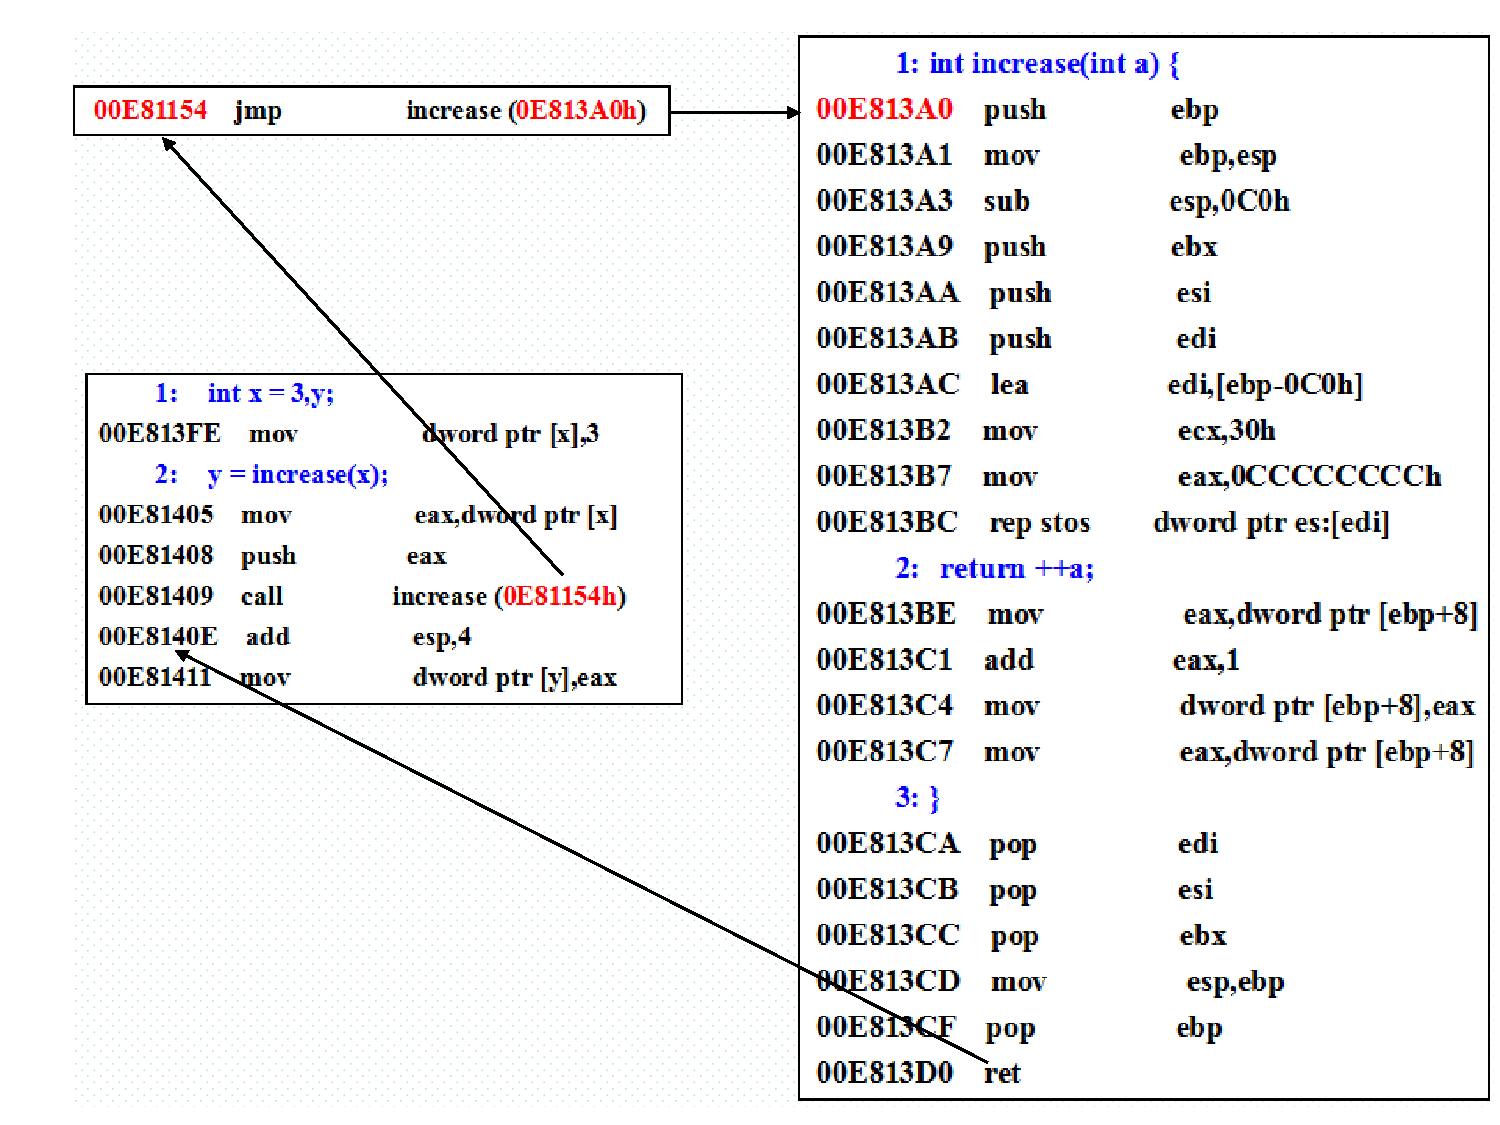
\includegraphics[width=0.8\textwidth]{chap02/03funasm}
    \end{minipage}
  \end{center}
\end{frame}
\subsection[内联函数]{内联函数}
\begin{frame}[fragile]{函数}{内联函数}
  \stretchon
  \begin{itemize}
  \item 普通函数调用缺陷
    \begin{itemize}
    \item 时间开销
    \end{itemize}
  \item 内联函数
    \begin{itemize}
    \item 在编译时将函数体代码插入到调用处
    \item 适用于代码短、频繁调用的场合
    \end{itemize}
  \item 定义\\[2ex]
    %\begin{center}
      \begin{minipage}{0.6\linewidth}
        \begin{cpptt}
inline |函数类型| |函数名|(|参数表|)
{
    |函数体|;
}
       \end{cpptt}
      \end{minipage}
    %\end{center}
  \end{itemize}
  \stretchoff
\end{frame}

\begin{frame}[fragile]{函数}{内联函数}
  \begin{itemize}
  \item 本质是预处理后展开\\
    \begin{center}
      \begin{minipage}{0.4\linewidth}
        \begin{cppcode}
inline int increase(int a)
{
  return ++a;
}
int main()
{
  int x = 3,y;
  y = increase(x);
  return 0;
}
        \end{cppcode}
      \end{minipage}$\Longrightarrow$
      \begin{minipage}{0.3\linewidth}
        \begin{cppcode}
int main()
{
  int x = 3,y;
  int a = x;
  y = ++a;
  return 0;
}
        \end{cppcode}
      \end{minipage}
    \end{center}
  \item 效率测试\\
    \begin{center}
      \begin{minipage}{0.56\linewidth}
        \begin{cppcode}
inline float getCos_inline(int &x)
{
  float r;
  x = rand();
  r = cos(2 * 3.1416 * x / (float)RAND_MAX);
  return r;
}
        \end{cppcode}
      \end{minipage}
      \begin{minipage}{0.4\linewidth}
        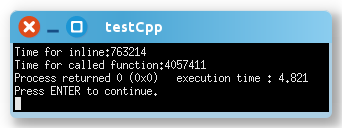
\includegraphics[width=0.8\textwidth]{chap02/04inlinetest}\\
        \tiny
        测试环境 (Code:Blocks GCC Release)\\
        效率比 = 4057411ms/763214ms = 5.3
        \colorbox{yellow}{\textcolor{blue}{例02-07:ex02-07.cpp}}
      \end{minipage}
    \end{center}
  \end{itemize}
\end{frame}

\begin{frame}[fragile]{函数}{内联函数}
  \stretchon
  \begin{itemize}
  \item 注意事项
    \begin{itemize}
    \item 不能出现递归
    \item 代码不宜过长
    \item 不宜出现循环
    \item 不宜含有复杂控制语句如\cppinttfts{switch}等
    \item 有些编译器会智能处理是否为内联函数
    \end{itemize}
  \end{itemize}
  \stretchoff
\end{frame}
\subsection[constexpr函数]{constexpr函数}
\begin{frame}[fragile]{函数}{constexpr函数}
  \stretchon
  \begin{itemize}
  \item 语法
    \begin{itemize}
    \item \cppinttfts{constexpr |\emph{函数}|(|\emph{常量表达式函数}|)}
    \end{itemize}
  \item 基本要求
    \begin{itemize}
    \item 只有一句\cppinttfts{return}可执行语句,可有别名、
      \cppinttfts{using}等
    \item 必须有返回类型,返回类型不能是\cppinttfts{void}
    \item 使用前必须定义(不只是声明)
    \item \cppinttfts{return}中不能有非常量表达式
    \end{itemize}
  \end{itemize}
  \stretchoff
\end{frame}

\begin{frame}[fragile]{函数}{constexpr函数}
  \stretchon
  \begin{itemize}
  \item 是编译时求值,不是运行是调用\\[-1.5ex]
    \begin{cppcode}
constexpr int data() // 错误,函数体只能有一条return可执行语句
{
  const int i = 1;
  return i;
}
constexpr int data() // 正确
{
  return 1;
}
constexpr void f()   // 错误,无法获得常量
{
}
    \end{cppcode}
  \item 是函数使用(\alert{编译时}),不是函数调用(\alert{运行时})\\[-1.5ex]
    \begin{cppcode}
constexpr int f();     // 只有constexpr函数的声明,没有定义
int a = f();           // 正确,可以将编译时的计算转换为运行时的调用
const int b = f();     // 正确,编译器将f()转换为一个运行时的调用
constexpr int c = f(); // 错误,c是constexpr,要求使用f(),在编译时计算
constexpr int f()      // constexpr函数的定义
{
  return 1;
}
constexpr int d = f(); // 正确,f()已定义,可以使用f()
    \end{cppcode}
  \end{itemize}
  \stretchoff
\end{frame}

\begin{frame}[fragile]{函数}{constexpr函数}
  \stretchon
  \begin{itemize}
  \item \cppinline{return}中不能包含运行时才能确定的函数\\[-1.5ex]
    \begin{cppcode}
const int e() 
{        
  return 1;
}
constexpr int g()
{
  return e();     // 错误,调用了非constexpr函数
}
constexpr int e() 
{        
  return 1;
}
constexpr int g() 
{
  return e();     // 正确,函数e()是常量表达式函数
}
    \end{cppcode}
  \item 用\cppinline{constexpr}函数初始化\cppinline{constexpr}变量\\[-1.5ex]
    \begin{cppcode}
constexpr int new_sz()
{
  return 100;
}
constexpr int size = new_sz();
    \end{cppcode}
  \end{itemize}
  \stretchoff
\end{frame}
\subsection[形参默认值]{形参默认值}
\begin{frame}[fragile]{函数}{带默认形参值的函数}
  \begin{spacing}{1.8}
    \begin{itemize}
    \item 在函数定义或说明中\alert{为形参赋默认值}
    \item 作用
      \begin{itemize}
      \item 若调用给出实参值,则形参采用实参值
      \item 若调用未给出实参值,则调用默认参数值
      \end{itemize}
    \end{itemize}
  \end{spacing}
  \vspace{-2ex}
  \begin{center}
    \begin{minipage}{0.9\linewidth}
      \cppfile{codes/chap02/ex02-08.cpp}
    \end{minipage}
  \end{center}
\end{frame}

\begin{frame}[fragile]{函数}{带默认形参值的函数}
  \begin{spacing}{1.8}
    \begin{itemize}
    \item \alert{基本要求}
      \begin{itemize}
        \scriptsize
      \item 调用函数时,如省去某个实参,则该实参右边所有实参都要省略
      \item 默认形参必须\alert{自最右向左连续}定义
      \item 若函数声明(原型)中给出默认形参值,则函数定义时不能重复指定
      \end{itemize}
    \end{itemize}
  \end{spacing}
  \vspace{-3ex}
  \begin{center}
    \begin{minipage}{0.9\linewidth}
      \cppfile{codes/chap02/ex02-09.cpp}
    \end{minipage}
  \end{center}
\end{frame}

\begin{frame}[fragile]{函数}{带默认形参值的函数}
  \begin{itemize}
  \item \alert{中间参数不能省略}
  \end{itemize}
  \begin{center}
    \begin{minipage}{0.9\linewidth}
      \begin{tikzpicture}[show background grid]
        %\tiny
        \umlnote[text width = 1.00\textwidth](code1) at (0, 0)
        {
          \cppfiletikz{codes/chap02/ex02-10.cpp}
        };
      \end{tikzpicture}
      %\cppfile{codes/chap02/ex02-10.cpp}
    \end{minipage}
  \end{center}
\end{frame}

\begin{frame}[fragile]{函数}{带默认形参值的函数}
  \begin{itemize}
  \item \alert{不可重复指定参数默认值}
  \end{itemize}
  \begin{center}
    \begin{minipage}{0.9\linewidth}
      \cppfile{codes/chap02/ex02-11.cpp}
    \end{minipage}
  \end{center}
\end{frame}

\begin{frame}[fragile]{函数}{带默认形参值的函数}
  \begin{itemize}
  \item 默认形参必须\alert{自最右向左连续}定义
  \end{itemize}
  \begin{center}
    \begin{minipage}{0.9\linewidth}
      \cppfile{codes/chap02/ex02-12.cpp}
    \end{minipage}
  \end{center}
\end{frame}

\begin{frame}[fragile]{函数}{带默认形参值的函数}
  \begin{itemize}
  \item 默认形参必须\alert{自最右向左连续}定义
  \end{itemize}
  \begin{center}
    \begin{minipage}{0.9\linewidth}
      \cppfile{codes/chap02/ex02-13.cpp}
    \end{minipage}
  \end{center}
\end{frame}

\begin{frame}[fragile]{函数}{带默认形参值的函数}
  \begin{itemize}
  \item 必须为无默认值的参数提供实参
  \end{itemize}
  \begin{center}
    \begin{minipage}{0.9\linewidth}
      \begin{tikzpicture}[show background grid]
        %\tiny
        \umlnote[text width = 1.0\textwidth](code1) at (0, 0)
        {
          \cppfiletikz{codes/chap02/ex02-14.cpp}
        };
      \end{tikzpicture}
      %\cppfile{codes/chap02/ex02-14.cpp}
    \end{minipage}
  \end{center}
\end{frame}

\begin{frame}[fragile]{函数}{带默认形参值的函数}
  \begin{itemize}
  \item 形参的初始化可以是函数
  \end{itemize}
  \begin{center}
    \begin{minipage}{0.9\linewidth}
      \cppfile{codes/chap02/ex02-15.cpp}
    \end{minipage}
  \end{center}
\end{frame}
\subsection[重载函数]{重载函数}
\begin{frame}[fragile]{函数}{函数重载}
  \stretchon
  \begin{itemize}
  \item 重载:同一符号或函数名对应多种操作
    \begin{itemize}
    \item 操作符重载
    \item 函数重载
    \end{itemize}
  \item 函数重载
    \begin{itemize}
    \item 共性函数拥有相同函数名字\\
      \begin{cppcode}
int sum_int(int *a, int size);
float sum_float(float *a, int size);
double sum_double(double *a, int size);
      \end{cppcode}
      \vspace{-2ex}
      \begin{cppcode}
int sum(int *a, int size);
float sum(float *a, int size);
double sum(double *a, int size);
      \end{cppcode}
    \end{itemize}
  \end{itemize}
  \stretchoff
\end{frame}

\begin{frame}[fragile]{函数}{函数重载}
  \stretchon
  \begin{itemize}
  \item C++函数重载实现机理
    \begin{itemize}
    \item 函数名
    \item 参数类型
    \item 参数个数
    \end{itemize}
  \item 参数个数不同情况下的实现重载
    \begin{itemize}
      \begin{cppcode}
float dis_2d(float x0, float y0, float x1, float y1);
float dis_3d(float x0, float y0, float z0,
             float x1, float y1, float z1);
      \end{cppcode}
      \vspace{-2ex}
      \begin{cppcode}
float dis(float x0, float y0, float x1, float y1);
float dis(float x0, float y0, float z0,
          float x1, float y1, float z1);
      \end{cppcode}
    \end{itemize}
  \end{itemize}
  \stretchoff
\end{frame}

\begin{frame}[fragile]{函数}{函数重载}
  \stretchon
  \begin{itemize}
  \item 注意事项
    \begin{itemize}
    \item 避免二义性\\
      %\begin{center}
        \begin{minipage}{0.5\linewidth}
          \begin{cppcode}
void my_fun(int a, int b);
void my_fun(int &a, int &b);
          \end{cppcode}
        \end{minipage}
      %\end{center}
    \item 避免将不适宜重载的函数重载\\
      {\tiny 如果不同的函数名所提供的信息可使程序更容易理解,则不必使用重载}
      %\begin{center}
        \begin{minipage}{0.5\linewidth}
          \begin{cppcode}
void rotate(float r);
void translate(float x, float y);
          \end{cppcode}
          \vspace{-2ex}
          \begin{cppcode}
void transform(float r);
void transform(float x, float y);
          \end{cppcode}
        \end{minipage}
      %\end{center}
    \end{itemize}
  \end{itemize}
  \stretchoff
\end{frame}
\subsection{函数模板}
\begin{frame}[fragile]{函数}{函数模板}
  \stretchon
  \begin{itemize}
  \item 用一个函数表示逻辑功能相同但参数类型不同的函数\\
    %\begin{center}
      \begin{minipage}{0.6\linewidth}
        \begin{cppcode}
int sum(int *a, int size);
float sum(float *a, int size);
double sum(double *a, int size);
        \end{cppcode}
      \end{minipage}
    %\end{center}
  \item 定义\\
    %\begin{center}
      \tiny
      \begin{minipage}{0.8\linewidth}
        \mintinline{cpp}{template <class} 类型名1,
        \mintinline{cpp}{class} 类型名1, \ldots \mintinline{cpp}{>}
        返回类型~函数名(形参表)\\
        \{\\
            函数体;\\
        \}
      \end{minipage}\\
      \begin{minipage}{0.6\linewidth}
        \cppfile{codes/chap02/ex02-16.cpp}
      \end{minipage}
    %\end{center}
    \end{itemize}
  \stretchoff  
\end{frame}

\begin{frame}[fragile]{函数}{函数模板}
  \begin{itemize}  
  \item 带有两个通用类型的函数模板\\
    \begin{center}      
      \begin{minipage}{0.6\linewidth}
        \cppfile{codes/chap02/ex02-17.cpp}
      \end{minipage}
    \end{center}
  \end{itemize}
\end{frame}

\begin{frame}[fragile]{函数}{函数模板}
  \stretchon
  \begin{itemize}  
  \item 优先级别
    \begin{itemize}
    \item 如果同时定义重载函数,将优先使用重载函数,若不能找到精确匹配,再使用函数模板
    \end{itemize}
  \item 应用
    \begin{itemize}
    \item 数据结构中的链表、堆栈等
    \item C++的标准模板库(排序等)
    \item 通用类
    \end{itemize}
  \end{itemize}
  \stretchoff
\end{frame}

\begin{frame}[fragile]{函数}{函数模板}
  \begin{itemize}  
  \item 应用(例:冒泡排序)\\
    \begin{center}      
      \begin{minipage}{0.6\linewidth}
        \cppfile{codes/chap02/ex02-18.cpp}
      \end{minipage}
    \end{center}
  \end{itemize}
\end{frame}
\subsection{系统函数}
\begin{frame}[fragile]{函数}{系统函数}
  \stretchon
  \begin{itemize}  
  \item cmath
  \item iostream
    \begin{itemize}
    \item 包含\cppinttfts{ctype.h, string.h, memory.h, stdlib.h}等
        \cppinttfts{isdigit(), strcpy(), memcpy(), atoi(), rand()}等
    \end{itemize}
  \item ctime
    \begin{itemize}
    \item \cppinttfts{time_t, clock()}等
    \end{itemize}
  \end{itemize}
  \stretchoff
\end{frame}  
%%%%%%%%%%%%%%%%%%%%%%%%%%%%%%%%%%%%%%%%%%%%%%%%%%%%%%%%%%%%%%%%%%%%%%%%%%


\section[程序结构]{大型程序结构控制}\label{sec:chap02-sec07}
%%%%%%%%%%%%%%%%%%%%%%%%%%%%%%%% 基本C++程序 %%%%%%%%%%%%%%%%%%%%%%%%%%%%%%%%%%
\begin{frame}[fragile]{程序结构}{extern和static}
  \begin{itemize}  
  \item \cppinline{extern}    
    \begin{itemize}
      \tiny
    \item 大型程序设计中所有模块共同使用的全局变量(函数)
    \item 在一个模块中定义全局变量(函数),其它模块中
      用\cppinttscr{extern}说明``外来''的全局变量(函数)
    \end{itemize}
  \end{itemize}
  \vspace{-4.5ex}
  \begin{columns}
    \centering
    \begin{column}{0.42\textwidth}
      \centering
      \cppfile{codes/chap02/ex02-19-01.cpp}%}
      \vspace{-6ex}
      \cppfile{codes/chap02/ex02-19-02.cpp}%}
    \end{column}
    \begin{column}{0.42\textwidth}
      \centering
      \cppfile{codes/chap02/ex02-19-00.cpp}\\[-0.5ex]%}
      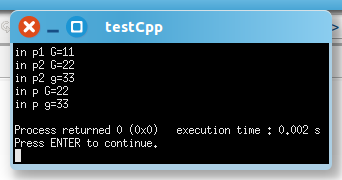
\includegraphics[width=0.8\textwidth]{chap02/05externkeyword}
    \end{column}
  \end{columns}
\end{frame}

\begin{frame}[fragile]{程序结构}{extern和static}
  \begin{itemize}  
  \item \cppinline{static}    
    \begin{itemize}
      \tiny
    \item \cppintttny{static}可用来声明全局静态变量和局部静态变量。当声明全局静态变
      量时,全局静态变量只能供本模块使用,不能被其它模块再声明
      为\cppintttny{extern}变量
    \end{itemize}
  \end{itemize}
  \begin{center}
    \begin{minipage}{0.4\linewidth}
      \cppfile{codes/chap02/ex02-20-01.cpp}
    \end{minipage}\qquad
    \begin{minipage}{0.4\linewidth}
      \cppfile{codes/chap02/ex02-20-02.cpp}
    \end{minipage}
  \end{center}
\end{frame}

\begin{frame}[fragile]{程序结构}{extern和static}
  \begin{itemize}  
  \item \cppinline{static}    
    \begin{itemize}
      \tiny
    \item 当一个局部变量声明为\cppintttny{static}变量,它既具有局部变量的性质,又具
      有全局变量的性质
    \end{itemize}
  \end{itemize}
  \begin{center}
    \begin{minipage}{0.53\linewidth}
      \cppfile{codes/chap02/ex02-21.cpp}
    \end{minipage}\qquad
    \begin{minipage}{0.35\linewidth}
      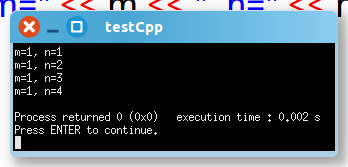
\includegraphics[width=0.8\textwidth]{chap02/06statickeyword}
    \end{minipage}
  \end{center}
\end{frame}

\begin{frame}[fragile]{程序结构}{包含头文件}
  \stretchon
  \begin{itemize}  
  \item 多文件操作使用\cppinline{#include}
  \item \cppintt{#include <|系统文件|>}
    \begin{itemize}
    \item 到编译器指定的文件包含目录查找
    \end{itemize}
  \item \cppintt{#include "|自定义文件.h"}
  \end{itemize}
  \stretchoff
\end{frame}

\begin{frame}[fragile]{程序结构}{条件编译}
  \begin{itemize}
  \item 同一程序在不同的编译条件下得到不同的目标代码
  \end{itemize}
  \begin{center}
    \begin{minipage}{0.6\linewidth}
      \cppfile{codes/chap02/ex02-22.cpp}
    \end{minipage}
  \end{center}
\end{frame}

\begin{frame}[fragile]{程序结构}{条件编译}
  \begin{itemize}
  \item 便于程序移植或跨平台
  \end{itemize}
  \begin{center}
    \begin{minipage}{0.4\linewidth}
      \cppfile{codes/chap02/ex02-23-01.cpp}
    \end{minipage}\qquad
    \begin{minipage}{0.4\linewidth}
      \cppfile{codes/chap02/ex02-23-02.cpp}
    \end{minipage}
  \end{center}
\end{frame}

\begin{frame}[fragile]{程序结构}{条件编译}
  \begin{itemize}
  \item 避免重复包含头文件如``MyHeader.h''\\
    \begin{center}
      \begin{minipage}{0.4\linewidth}
        \cppfile{codes/chap02/ex02-24.cpp}
      \end{minipage}
    \end{center}
  \item 便于调试程序\\
    \begin{center}
      \begin{minipage}{0.4\linewidth}
        \cppfile{codes/chap02/ex02-25.cpp}
      \end{minipage}
    \end{center}
  \end{itemize}
\end{frame}

\begin{frame}[fragile]{程序结构}{名字空间}
  \stretchon
  \begin{itemize}
  \item 不同程序员撰写的软件模块可能使用相同标志符
  \item 为避免冲突,将可能存在相同标志符的程序模块放入名字空间
  \item 定义:\\
    %\begin{center}
    \begin{minipage}{0.8\linewidth}
      \begin{cpptt}
namespace |名称|
{
   |成员变量或成员函数|;
}
        \end{cpptt}
      \end{minipage}
    %\end{center}    
    \end{itemize}
    \stretchoff
\end{frame}

\begin{frame}[fragile]{程序结构}{名字空间}
  \begin{itemize}
  \item 声明方式(作用域分辨符)\\
    名字空间名\cppinline{::}成员变量或成员函数\\
    \begin{center}
      \begin{minipage}{0.45\linewidth}
        \cppfile{codes/chap02/ex02-25-02.h}
      \end{minipage}\qquad
      \begin{minipage}{0.45\linewidth}
        \cppfile{codes/chap02/ex02-25-01.cpp}
      \end{minipage}
    \end{center}    
  \end{itemize}
\end{frame}

\begin{frame}[fragile]{程序结构}{名字空间}%label=testframe,
  \begin{itemize}
  \item 声明方式(作用域分辨符)\\
    名字空间名\cppinline{::}成员变量或成员函数\\
    \begin{center}
      \begin{minipage}{0.45\linewidth}
        \cppfile{codes/chap02/ex02-26-02.h}
      \end{minipage}\qquad
      \begin{minipage}{0.45\linewidth}
        \cppfile{codes/chap02/ex02-26-01.cpp}
      \end{minipage}
    \end{center}    
  \end{itemize}
\end{frame}

%%%%%%%%%%%%%%%%%%%%%%%%%%%%%%%%%%%%%%%%%%%%%%%%%%%%%%%%%%%%%%%%%%%%%%%%%%

% 附件页
\section[附件下载]{本讲示例代码及附件下载} 
\begin{frame}{附件}{本讲附件}
  % 此处的[ucfilespec=...]必须指定为pdf否则Windows下无法下载
  %\vspace{-4ex}
  \textattachfile[ucfilespec=ex-src02.pdf]{ex-src02.zip}{附件:右键单击该
    链接,选择\qtmark{\alert{保存附件}}下载,\alert{将后缀名改为\qtmark{.zip}解压}
      \footnote[frame]{请\alert{退出全屏模式}后点击该链接。}
      \footnote[frame]{以Adobe Acrobat Reader为例。}
      。}%\\

  \vspace{-1ex}
  \begin{center}
    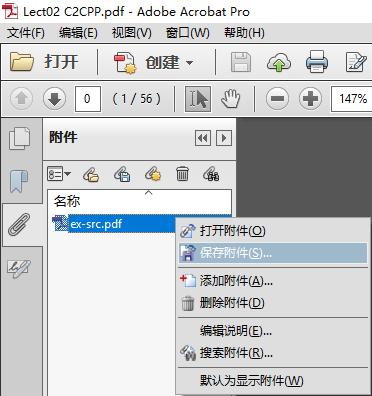
\includegraphics[height=0.35\textheight]{pdfattatchdownload01}\quad
    %或 \quad%
    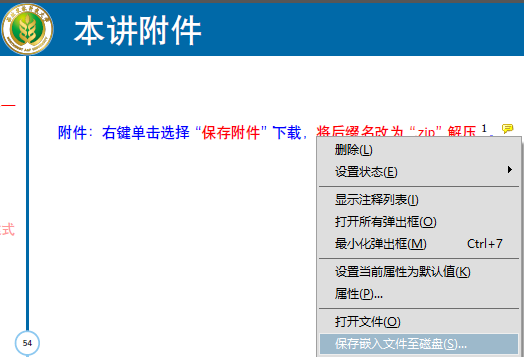
\includegraphics[height=0.35\textheight]{pdfattatchdownload02}\\[2ex]%
    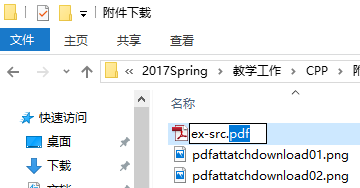
\includegraphics[height=0.255\textheight]{pdfattatchdownload03}\quad
    %$\Rightarrow$ \quad%
    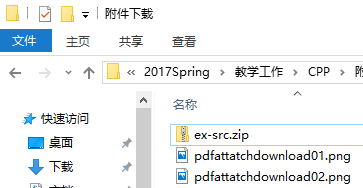
\includegraphics[height=0.255\textheight]{pdfattatchdownload04}%
  \end{center}   
\end{frame}

% \tiny
% \scriptsize
% \footnotesize
% \small
% \normalsize
% \large
% \Large
% \LARGE
% \huge
% \Huge


%%% Local Variables: 
%%% mode: latex
%%% TeX-master: "../main.tex"
%%% End: 
 % 算法
  \or % 第3章
    \lecture{类和对象}{lec:chap03}
\section[概念]{类和对象的概念}\label{sec:chap03-sec01}
%%%%%%%%%%%%%%%%%%%%%%%%%%%%%% 类和对象的概念 %%%%%%%%%%%%%%%%%%%%%%%%%%%%%%%%%%
%%\subsection[新结构体]{从C结构体到C++新结构体}\label{sec:chap03-sec01-01}
%%%%%%%%%%%%%%%%%%%%%%%%%%%%%% 从C结构体到C++新结
%%%%%%%%%%%%%%%%%%%%%%%%%%%%%% 构%%%%%%%%%%%%%%%%%%%%%%%%%%%%%%
\subsection[结构体]{结构体的演化}
\begin{frame}[fragile]{类和对象}{C结构体定义与使用}%
  \begin{itemize}
  \item 将不同数据类型组合成一个整体\\
    \begin{center}
      \begin{minipage}{0.45\linewidth}
        \begin{cpptcb}[||]{语法}
struct |结构类型名|
{
    |数据类型1 成员变量1|;
    |数据类型2 成员变量2|;
    |…|
    |数据类型n 成员变量n|;
};
        \end{cpptcb}
      \end{minipage}\qquad
      \begin{minipage}{0.38\linewidth}
        \begin{cpptcb}{定义}
struct StuNode{
    int ID;
    char name[20];
    char gender[12];
    int age;
};
        \end{cpptcb}
      \end{minipage}
    \end{center} 
  \item 结构体的实际大小\\
    {\tiny 有时$\neq$结构体内部成员变量所占内存之和}\\
    \begin{center}
      \begin{minipage}{0.45\linewidth}%x|\colorbox{green}{**}|2
        \begin{cpptcb}[||]{字节数}
sizeof(StuNode) = |\colorbox{green}{40}|;

2*sizeof(int)
+sizeof(char)*(20+|\colorbox{green}{12}|)
= |\colorbox{green}{40}|;
        \end{cpptcb}
      \end{minipage}\qquad
      \begin{minipage}{0.38\linewidth}
        \begin{cpptcb}{定义}
struct StuNode{
    int ID;
    char name[20];
    char gender[12];
    int age;
};
        \end{cpptcb}
      \end{minipage}
    \end{center}
  \end{itemize}
\end{frame}

\begin{frame}[fragile]{类和对象}{C结构体定义与使用}%
  \begin{spacing}{1.3}
  \begin{itemize}
  \item 结构体的实际大小\\
    {\tiny 有时$\neq$结构体内部成员变量所占内存之和}\\
    \begin{center}
      \begin{minipage}{0.45\linewidth}
        \begin{cpptcb}[||]{字节数}
sizeof(StuNode) = |\colorbox{green}{44}|;

2*sizeof(int)
+sizeof(char)*(20+|\colorbox{green}{13}|)
= |\colorbox{green}{41}|;
        \end{cpptcb}
      \end{minipage}\qquad
      \begin{minipage}{0.38\linewidth}
        \begin{cpptcb}{定义}
struct StuNode{
    int ID;
    char name[20];
    char gender[13];
    int age;
};
        \end{cpptcb}
      \end{minipage}\\
      \begin{minipage}{0.45\linewidth}
        \begin{cpptcb}[||]{字节数}
sizeof(StuNode) = |\colorbox{green}{44}|;

2*sizeof(int)
+sizeof(char)*(20+|\colorbox{green}{15}|)
= |\colorbox{green}{43}|;
        \end{cpptcb}
      \end{minipage}\qquad
      \begin{minipage}{0.38\linewidth}
        \begin{cpptcb}{定义}
struct StuNode{
    int ID;
    char name[20];
    char gender[15];
    int age;
};
        \end{cpptcb}
      \end{minipage}
    \end{center}
  \end{itemize}
  \end{spacing}
\end{frame}

\begin{frame}[fragile]{类和对象}{C结构体定义与使用}%
  \begin{spacing}{1.2}
  \begin{itemize}
  \item 结构体的实际大小\\
    {\tiny
      \cppintttny{SumSize} = 结构体内部成员变量所占内存之和\\
      \cppintttny{L} = 结构体内基本类型长度的最大值\\
      \cppintttny{SumSize % L == 0 ? SumSize : (L * (SumSize / L) % + L)}
      }
      \begin{center}
        \begin{minipage}{0.45\linewidth}
        \begin{cpptcb}[||]{字节数}
sizeof(StuNode) = |\colorbox{green}{44}|;

2*sizeof(int)
+sizeof(char)*(20+|\colorbox{green}{16}|)
= |\colorbox{green}{44}|;
        \end{cpptcb}
      \end{minipage}\qquad
      \begin{minipage}{0.38\linewidth}
        \begin{cpptcb}{定义}
struct StuNode{
    int ID;
    char name[20];
    char gender[16];
    int age;
};
        \end{cpptcb}
      \end{minipage}\\          
      \begin{minipage}{0.6\linewidth}
        \begin{cpptt}
|设置内存\emph{对齐方式}:|#pragam pack(value)
        \end{cpptt}
      \end{minipage}\\
      \begin{minipage}{0.6\linewidth}
        \begin{cppcode}
#pragma pack(1)
        \end{cppcode}
      \end{minipage}      
    \end{center}
  \end{itemize}
  \end{spacing}
\end{frame}

\begin{frame}[fragile]{类和对象}{结构体的使用}%
  \begin{spacing}{1.5}
  \begin{itemize}
  \item 结构体的使用\\[4ex]
    \begin{center}
      \begin{minipage}{0.55\linewidth}
        \begin{cpptcb}[||]{语法}
struct |结构类型名 结构变量名| = {
  |成员1初始值|,
  |成员2初始值|,
  |\ldots|,
  |成员n初始值|
};
        \end{cpptcb}
      \end{minipage}\qquad
      \begin{minipage}{0.35\linewidth}
        \begin{cpptcb}{定义}
struct StuNode{
  int ID;
  char name[20];
  char gender[16];
  int age;
};
        \end{cpptcb}
      \end{minipage}\\
      \vspace{4ex}
      \begin{minipage}{0.85\linewidth}
        \begin{cpptcb}{声明}
struct StuNode myNode0;
struct StuNode myNode = {101,"Tom","male",35};
        \end{cpptcb}
      \end{minipage}
    \end{center}
  \end{itemize}
  \end{spacing}
\end{frame}

% \begin{frame}[fragile]{类和对象}{结构体的使用}%
%   \begin{itemize}
%   \item 结构体的使用\\
%     \begin{center}
%       \begin{minipage}{0.45\linewidth}
%         \begin{cpptt}
%           struct |结构类型名 结构变量名| = {
%             |成员1初始值|,
%             |成员2初始值|,
%             |\ldots|,
%             |成员n初始值|
%           };
%         \end{cpptt}
%       \end{minipage}\qquad
%       \begin{minipage}{0.45\linewidth}
%         \begin{cppcode}
%           struct StuNode{
%             int ID;
%             char name[20];
%             char gender[16];
%             int age;
%           };
%         \end{cppcode}
%       \end{minipage}\\
%       \vspace{4ex}
%       \begin{minipage}{0.8\linewidth}
%         \begin{cpptt}
%           typedef struct |结构类型名 \colorbox{green}{结构类型别名}|;
%         \end{cpptt}
%       \end{minipage}\\
%       \begin{minipage}{0.8\linewidth}
%         \begin{cppcode}
%           typedef struct StuNode Stu_Node;
%           Stu_Node myNode0;
%           Stu_Node myNode = {101,"Tom","male",35};
%         \end{cppcode}
%       \end{minipage}
%     \end{center}
%   \end{itemize}
% \end{frame}

% \begin{frame}[t, fragile]{类和对象}{结构体的使用}%
%   \begin{itemize}
%   \item 结构体的使用\\
%     \begin{center}
%       \begin{minipage}{0.6\linewidth}
%         \begin{cpptt}
%           typedef struct  |结构类型名| = {
%             |数据类型1 成员变量1|;
%             |数据类型2 成员变量2|;
%             |\ldots|;
%             |数据类型n 成员变量n|;
%           }|\colorbox{green}{结构类型别名}|;
%         \end{cpptt}
%       \end{minipage}\\
%       \begin{minipage}{0.45\linewidth}
%         \begin{cppcode}
%           struct StuNode{
%             int ID;
%             char name[20];
%             char gender[16];
%             int age;
%           };
%         \end{cppcode}
%       \end{minipage}\qquad
%       \begin{minipage}{0.45\linewidth}
%         \begin{cppcode}
%           typedef struct StuNode{
%             int ID;
%             char name[20];
%             char gender[16];
%             int age;
%           }Stu_Node;
%         \end{cppcode}
%       \end{minipage}\\
%       \vspace{2ex}      
%       \begin{minipage}{0.8\linewidth}
%         \begin{cppcode}
%           Stu_Node myNode0;
%           Stu_Node myNode = {101,"Tom","male",35};
%         \end{cppcode}
%       \end{minipage}
%     \end{center}
%   \end{itemize}
% \end{frame}

% \begin{frame}[t, fragile]{类和对象}{结构体的使用}%
%   \begin{itemize}
%   \item 链表、队列与堆栈\\
%     \begin{center}      
%       \begin{minipage}{0.45\linewidth}
%         \begin{cppcode}
%           struct StuNode{
%             int ID;
%             char name[20];
%             char gender[16];
%             int age;
%             struct StuNode *next;
%           };
%         \end{cppcode}
%       \end{minipage}
%     \end{center}
%   \item 双链表、二叉树和图\\
%     \begin{center}
%       \begin{minipage}{0.3\linewidth}
%         \begin{cppcode}
%           struct DList{
%             int data;
%             struct DList *back;
%             struct DList *next;
%           };
%         \end{cppcode}
%       \end{minipage}\quad
%       \begin{minipage}{0.3\linewidth}
%         \begin{cppcode}
%           struct BTree{
%             int data;
%             struct BTree *left;
%             struct BTree *right;
%           };
%         \end{cppcode}
%       \end{minipage}\quad
%       \begin{minipage}{0.3\linewidth}
%         \begin{cppcode}
%           struct Edge{
%             int marked;
%             int v0, v1;
%             struct Edge *e0;
%             struct Edge *e1;
%           };
%         \end{cppcode}
%       \end{minipage}
%     \end{center}
%   \end{itemize}
% \end{frame}

\begin{frame}[fragile]{类和对象}{C++新结构体}%
  \begin{itemize}
  \item 结构体中可以有函数%\\[1ex]
    \begin{center}
      \begin{minipage}{0.5\linewidth}
        \begin{tikzpicture}[show background grid]
          \node[scale = 0.78, text width = 1.0\textwidth](code1) at (0, 0)
          {
            \begin{cpptcb}[||]{语法}
struct |结构类型名| {
  |数据类型1 成员变量1|;
  |\ldots|;
  |数据类型n 成员变量n|;
  |\textcolor{red}{函数返回类型 函数名(参数列表)}|;
};
            \end{cpptcb}
          };          
          \umlnote[scale = 0.780, text width = 1.0\textwidth, below=0.1 of code1](code2)
          {
            \cppfiletikz{codes/chap03/ex03-01.cpp}
          };          
        \end{tikzpicture}
        %\scalebox{0.8}{\cppfile{codes/chap03/ex03-01.cpp}}
      \end{minipage}
    \end{center}
  \end{itemize}
\end{frame}

\begin{frame}[fragile]{类和对象}{C++新结构体}%
  \begin{itemize}
  \item 结构体中可以有函数\\[2ex]
    \begin{center}      
      \begin{minipage}{0.55\linewidth}
        \begin{tikzpicture}[show background grid, every node/.style={scale=1.2}]
          \tiny
          \umlnote[text width = 1.0\textwidth](code1) at (0, 0)
          {
            \cppfiletikz{codes/chap03/ex03-02.cpp}
          };          
        \end{tikzpicture}
        %\cppfile{codes/chap03/ex03-02.cpp}
      \end{minipage}
    \end{center}
  \end{itemize}
\end{frame}

\begin{frame}[fragile]{类和对象}{C++新结构体}%
  \begin{itemize}
  \item 新结构体的使用\\
    \begin{center}
      \begin{minipage}{0.41\linewidth}
        \begin{cpptt}
struct |结构类型名| {
  |数据类型1 成员变量1|;
  |数据类型2 成员变量2|;
  |\ldots|;
  |数据类型n 成员变量n|;
  |\textcolor{red}{函数返回类型 函数名(参数列表)}|;
};

|\tikzmark{ignorestructa}\textcolor{red}{[struct]} 结构类型名 变量名|;          
        \end{cpptt}
        %\vspace{-4ex}
        \textcolor{red}{\tiny \\ \hspace{4em} \tikzmark{ignorestructb}
          C++中可以省略}
        \begin{tikzpicture}[overlay,remember picture]
          \draw[->] (pic cs:ignorestructa) .. controls +(-1.5em, 0.1em)
          ..($ (pic cs:ignorestructb) +(0,0.2ex) $);
        \end{tikzpicture}
      \end{minipage}\quad
      %\vspace{-3ex}
      \begin{minipage}{0.54\linewidth}
        \begin{tikzpicture}[every node/.style={scale=1.1}]
          \tiny
          \umlnote[text width = 0.85\textwidth]
          {
            \cppfiletikz{codes/chap03/ex03-03.cpp}
          };          
        \end{tikzpicture}
        %\cppfile{codes/chap03/ex03-03.cpp}
      \end{minipage}
    \end{center}    
  \end{itemize}  
\end{frame}

\subsection[Graph2D]{Graph2D}
\begin{frame}[fragile]{类和对象}{C++新结构体应用实例}%
  \begin{itemize}
  \item \cppinline{Graph2D}功能结构\footnote[frame]{详情请参考软件包中的\alert{Graph2D Specification V1.0.pdf}文件}\\[4ex]
    \begin{center}
      \begin{minipage}{0.8\linewidth}
        \begin{tikzpicture}[font=\footnotesize, >=stealth, every node/.style={rounded
            corners, draw, minimum size=0.45cm}, level
          1/.style={sibling distance = 1cm}]          
          \node {\mintinline{cpp}{Graph2D}} [edge from parent fork
          down]
          child {node [below] {\parbox{1em}{图形初始化}}}
          child {node [below] {\parbox{1em}{窗口设置}}}
          child {node [below] {\parbox{1em}{基本图元绘制}}}
          child {node [below] {\parbox{1em}{字体创建与显示}}}
          child {node [below] {\parbox{1em}{图像读入与显示}}}
          child {node [below] {\parbox{1em}{键盘交互}}}
          child {node [below] {\parbox{1em}{鼠标交互}}}          
          child {node [below] {\parbox{1em}{其它}} 
          };
        \end{tikzpicture}
      \end{minipage}
    \end{center}
  \end{itemize}
\end{frame}

\begin{frame}[fragile]{类和对象}{C++新结构体应用实例}%
  \begin{itemize}
  \item \cppinline{Graph2D}运行机制
    \begin{center}
      \begin{minipage}{0.8\linewidth}
        \centering
        \scalebox{0.95}{
        \begin{tikzpicture}[%
          font=\tiny,
          >=triangle 60, % Nice arrows; your taste may be different
          %start chain=going below, % General flow is top-to-bottom
          node distance=3mm and 30mm, % Global setup of box spacing
          %every join/.style={norm}, % Default linetype for connecting boxes
          ]
          % -------------------------------------------------
          %A few box styles <on chain> *and* <on grid> reduce the need for
          % manual relative positioning of nodes
          %  Start by placing the nodes
          \node [term, densely dotted] {图形初始化\\添加回调函数};
          % Use join to connect a node to the previous one
          \node [proc, join] (p0) {keyboard回调函数\\处理键盘消息};
          \node [test, join] (t1) {退出?};
          \node [proc, join] (p1) {mouse回调函数\\处理鼠标消息};
          %\node [test, right=5 of p0] (p3) {退出?};
          \node [test, join] (t2) {退出?};
          \node [proc, join]  (p2) {display回调函数\\绘制更新图形};
          \node [term, densely dotted, below=1 of p2] (p3) {退出窗口};
          
          % Now we place the coordinate nodes for the connectors with
          % angles, or with annotations.
          \node [coord, right=of t1] (c1) {};
          \node [coord, right=of t2] (c2) {};
          \node [coord, above=0.5 of p3] (c3) {};
          \node [coord, left=of p0] (c4) {};
          \node [coord, left=of p2] (c5) {};
          % -------------------------------------------------

          \path (t1.south) to node [near start, xshift=1em] {否}
          (p1);
          \path (t2.south) to node [near start, xshift=1em] {否}
          (p2);
          \path (t1.east) to node [near start, yshift=1em] {是} (c1);
          \path (t2.east) to node [near start, yshift=1em] {是} (c2);
          \draw [->,lcnorm] (t1.east) -- (c1) |- (c2) |- (c3) --
          (p3.north);
          \draw [->,lcnorm] (t2.east) |- (c2) ;
          \draw [->,lcnorm] (p2.west) -- (c5) -- (c4) -- (p0.west) ;
        \end{tikzpicture}
        }
      \end{minipage}
    \end{center}
  \end{itemize}
\end{frame}

\begin{frame}[fragile]{类和对象}{C++新结构体应用实例}%
  \begin{itemize}
  \item \cppinline{Graph2D}坐标系统(二维笛卡尔右手坐标系)\\[2ex]
      \begin{center}
        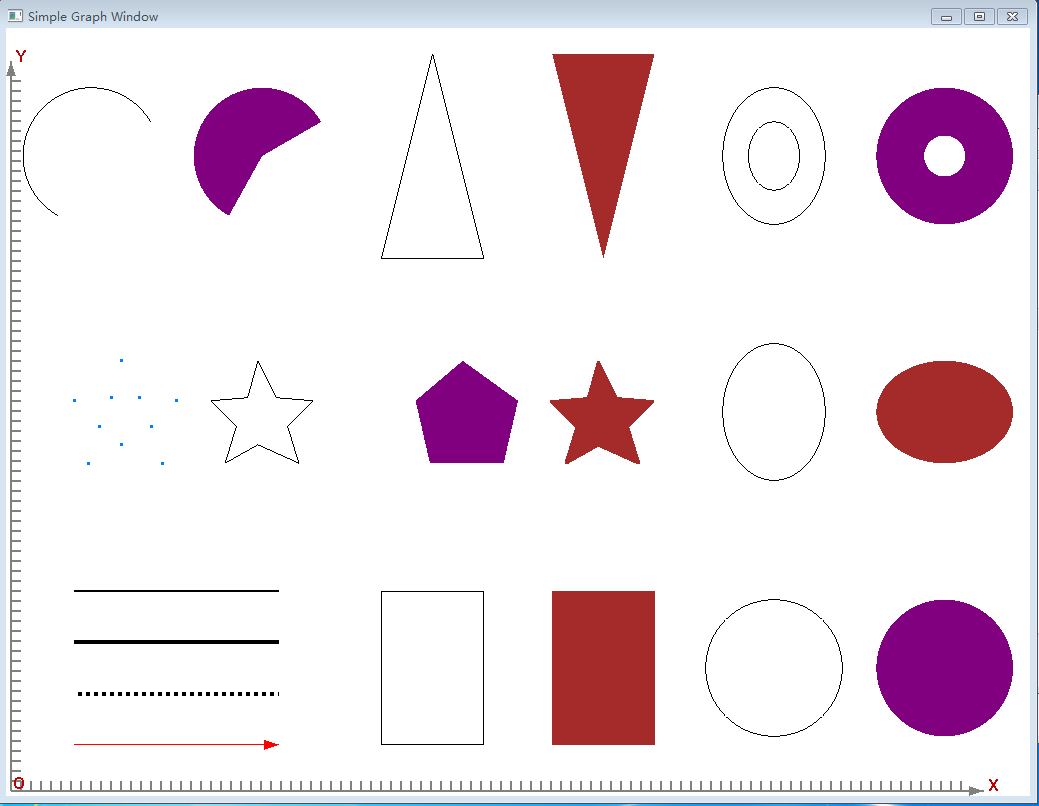
\includegraphics[height=0.75\textheight]{chap03/01graph2dcoord}
      \end{center}
  \end{itemize}
\end{frame}

\begin{frame}[fragile]{类和对象}{C++新结构体应用实例}%
  \begin{spacing}{1.2}
  \begin{itemize}  
  \item 图形库的安装
    \begin{itemize}
    \item \cppinline{Graph2D}库包含三个文件
      \begin{itemize}
      \item \cppinttfts{graph2d.h}
      \item \cppinttfts{libgraph2d.a}
      \item \cppinttfts{graph2d.dll} 
      \end{itemize}
    \item 安装
      \begin{itemize}
      \item 手动安装:参见Readme.txt文件
      \item 自动安装:运行InstallGraph2D.exe
        \begin{center}
          \vspace{1ex}
          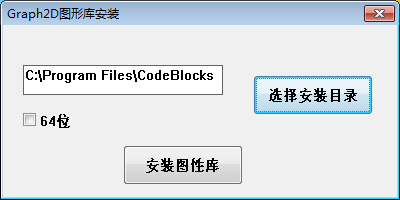
\includegraphics[height=0.4\textheight]{chap03/02graph2dinstall}
        \end{center}
      \end{itemize}
    \end{itemize}
  \end{itemize}
  \end{spacing}
\end{frame}

\begin{frame}[fragile]{类和对象}{C++新结构体应用实例}%
  \begin{itemize}  
  \item 图形库在\cppinline{Code::blocks}中的配置
      \begin{itemize}
      \item 在菜单 \menu{Settings>Compiler>Link settings} 中添加 \alert{libgdi32}、\alert{libopengl32}、\alert{libglu32}、
        \alert{libfreeglut} 和 \alert{libgraph2d}
        \begin{center}
          \vspace{2ex}
          \begin{overpic}[scale=.35,unit=1mm]%
            {chap03/03graph2dCBsetting}
            \put(18,23){\footnotesize \textcolor{red}{设置链接库}}
          \end{overpic}
        \end{center}
      \end{itemize}
  \end{itemize}
\end{frame}

\begin{frame}{类和对象}{C++新结构体应用实例}%
  \stretchon
  \begin{itemize}  
  \item Graph2D图形库\cppinline{Code::Blocks}开发向导\footnote[frame]{详见:\url{https://gitee.com/registor/Graph2D}}
      \begin{itemize}
      \item 将\texttt{devLibs}文件夹及其中所有文件\alert{保持目录结构}
        拷贝到任意位置(如C盘根目录)
      \item 将\texttt{Graph2D}文件夹和\texttt{config.script}复制到
        Code::Blocks安装目录的\texttt{wizard}文件夹\footnote[frame]{
        如:\texttt{C:\textbackslash Program Files (x86)\textbackslash CodeBlocks\textbackslash share\textbackslash CodeBlocks\textbackslash templates\textbackslash wizard}}
      \item 在菜单 \menu{Settings>Global variables...} 中添加
        \alert{cppg2d}和\alert{freeglut}环境变量\footnote[frame]{
        注意要与\texttt{devLibs}在自己硬盘上的路径一致}
      \end{itemize}
  \end{itemize}
  \centering  
  %\begin{center}
    \includegraphics[height=0.35\textheight]{chap03/cppg2d}
    \includegraphics[height=0.35\textheight]{chap03/freeglut}
  %\end{center}
  \stretchoff
\end{frame}

\begin{frame}{类和对象}{C++新结构体应用实例}%
  \stretchon
  \begin{itemize}  
  \item Graph2D图形库\cppinline{Code::Blocks}开发向导\footnote[frame]{详见:\url{https://gitee.com/registor/Graph2D}}
      \begin{itemize}
      \item 在向导中选择\texttt{Graph2D application}     
      \end{itemize}
  \end{itemize}
  \centering
  %\begin{center}
    \includegraphics[height=0.6\textheight]{chap03/cppg2dwizard}
  %\end{center}
  \stretchoff
\end{frame}

\begin{frame}[fragile]{类和对象}{C++新结构体应用实例}%
  \begin{spacing}{1.4}
    \begin{itemize}
    \item \cppinline{Graph2D}骆驼式命名法
      \begin{itemize}
      \item 第一个单词小写
      \item 后面的单词首字母大写
      \item 示例:\cppinttfts{showCoordinate}
      \end{itemize}
    \end{itemize}
  \end{spacing}
  \vspace{-2ex}
  \begin{center}
    \hspace{1em}
    \begin{minipage}{0.5\linewidth}
      \cppfile{codes/chap03/ex03-35.cpp}
    \end{minipage}\quad
    \begin{minipage}{0.4\linewidth}
      \begin{overpic}[scale=.15,unit=1mm]%
        {chap03/04graph2d1stpic}
      \end{overpic}      
    \end{minipage}    
  \end{center}
\end{frame}

\begin{frame}[fragile]{类和对象}{C++新结构体应用实例}%
  \begin{itemize}
  \item \cppinline{Graph2D}简单图形库的使用\\[2ex]
    \begin{center}
      \begin{minipage}{0.45\linewidth}
        \cppfile{codes/chap03/ex03-03-01.cpp}
      \end{minipage}\qquad
      \begin{minipage}{0.43\linewidth}
        \cppfile{codes/chap03/ex03-03-02.cpp}
      \end{minipage}
    \end{center}    
  \end{itemize}
\end{frame}

\begin{frame}{类和对象}{C++新结构体应用实例}%
  \stretchon
  \begin{itemize}
  \item \texttt{Graph2D}简单图形库的使用    
  \end{itemize}
  \centering
  \includegraphics[height=0.8\textheight]{chap03/leopard}
  \stretchoff
\end{frame}

\subsection[类和对象]{从面向过程到面向对象}
%%%%%%%%%%%%%%%%%%%%%%%%%%%%%% 从面向过程到面向对象 %%%%%%%%%%%%%%%%%%%%%%%%%%%%%%%%%%
\begin{frame}[fragile]{类和对象}{从面向过程到面向对象}%
  \stretchon
  \begin{itemize}
  \item 面向过程程序设计
    \begin{itemize}
    \item 程序模块由函数(过程)组成
    \item 数据与函数分离,通过参数传递给函数
    \end{itemize}
  \item 面向对象程序设计
    \begin{itemize}
    \item 程序模块由类组成
    \item 函数与数据是一个整体(封装)
    \item 访问限制
    \item 继承与多态性
    \end{itemize}
  \end{itemize}
  \stretchoff
\end{frame}

% \begin{frame}[t, fragile]{类和对象}{面向过程程序设计}%
%   \begin{itemize}
%   \item 分配一个空间,添加一个数据
%   \end{itemize}
%   \raggedright
%   \begin{minipage}[b]{0.25\linewidth}
%     \tiny
%     \begin{bytefield}{16}
%       \memsection[a]{$\rightarrow$}{}{1}{100}
%     \end{bytefield}
%   \end{minipage}\quad
%   \begin{minipage}[b]{0.25\linewidth}
%     \tiny
%     \begin{bytefield}{16}
%       \memsection[a]{$\rightarrow$}{}{1}{100}\\
%       \memsection{}{}{1}{99}
%     \end{bytefield}
%   \end{minipage}\\%\quad
%   % \begin{minipage}[b]{0.25\linewidth}
%   %   \tiny
%   %   \begin{bytefield}{16}
%   %     \memsection[a]{$\rightarrow$}{}{1}{100}\\
%   %     \memsection{}{}{1}{99}\\
%   %     \memsection{}{}{1}{98}
%   %   \end{bytefield}
%   % \end{minipage}\\
%   \vspace{2ex}
%   \hspace{1em}
%   \begin{minipage}{0.46\linewidth}
%     \cppfile{codes/chap03/ex03-04.cpp}
%   \end{minipage}\qquad
%   \begin{minipage}{0.4\linewidth}
%     \cppfile{codes/chap03/ex03-05.cpp}\\
%     \vfill
%     \alert{\tiny 内存分配与释放操作频繁}
%   \end{minipage}
% \end{frame}

% \begin{frame}[t, fragile]{类和对象}{面向过程程序设计}%
%   \begin{itemize}
%   \item 预先分配大块内存
%   \end{itemize}
%   \vspace{4ex}
%   \begin{minipage}[b]{0.2\linewidth}
%     \tiny
%     \begin{bytefield}{16}
%       \memsection[a]{$\rightarrow$}{}{1}{100}\\
%       \memsection{}{}{1}{\ldots}\\
%       \memsection{}{}{1}{\ldots}\\
%       \memsection{}{}{1}{\ldots}\\
%       \memsection{}{}{1}{\ldots}\\
%       \memsection{}{}{1}{\ldots}\\
%       \memsection{}{}{1}{\ldots}\\
%       \memsection{}{}{1}{\ldots}\\
%       \memsection{}{}{1}{\ldots}\\
%       \memsection{}{}{1}{\ldots}
%     \end{bytefield}
%   \end{minipage}\qquad
%   \begin{minipage}[b]{0.2\linewidth}
%     \tiny
%     \begin{bytefield}{16}
%       \memsection[a]{$\rightarrow$}{}{1}{100}\\
%       \memsection{}{}{1}{99}\\
%       \memsection{}{}{1}{98}\\
%       \memsection{}{}{1}{97}\\
%       \memsection{}{}{1}{96}\\
%       \memsection{}{}{1}{95}\\
%       \memsection{}{}{1}{94}\\
%       \memsection{}{}{1}{93}\\
%       \memsection{}{}{1}{92}\\
%       \memsection{}{}{1}{91}\\
%       \memsection{}{}{1}{\colorbox{green}{90}}
%     \end{bytefield}
%   \end{minipage}\\
%   \begin{center}
%     \begin{minipage}{0.5\linewidth}
%       \alert{\small 如果添加数据量小,浪费空间;\\
%         如果添加数据量太大,溢出。}
%     \end{minipage}
%   \end{center}
% \end{frame}

% \begin{frame}[t, fragile]{类和对象}{面向过程程序设计}%
%   \begin{itemize}
%   \item 按数据块进行分配
%   \end{itemize}
%   \vspace{6ex}
%   \hspace{-4em}
%   \begin{minipage}[b]{0.2\linewidth}
%     \tiny
%     \begin{bytefield}{16}
%       \memsection[a]{$\rightarrow$}{}{1}{100}\\
%       \memsection{}{}{1}{\ldots}\\
%       \memsection{}{}{1}{\ldots}\\
%       \memsection{}{}{1}{\ldots}\\
%       \memsection{}{}{1}{\ldots}
%     \end{bytefield}
%   \end{minipage}\qquad
%   \begin{minipage}[b]{0.2\linewidth}
%     \tiny
%     \begin{bytefield}{16}
%       \memsection[a]{$\rightarrow$}{}{1}{100}\\
%       \memsection{}{}{1}{99}\\
%       \memsection{}{}{1}{98}\\
%       \memsection{}{}{1}{97}\\
%       \memsection{}{}{1}{96}\\
%       \memsection{}{}{1}{\colorbox{red}{95}}
%     \end{bytefield}
%   \end{minipage}\qquad
%   \begin{minipage}[b]{0.2\linewidth}
%     \tiny
%     \begin{bytefield}{16}
%       \memsection[a]{$\rightarrow$}{}{1}{100}\\
%       \memsection{}{}{1}{99}\\
%       \memsection{}{}{1}{98}\\
%       \memsection{}{}{1}{97}\\
%       \memsection{}{}{1}{96}\\
%       \memsection{}{}{1}{\colorbox{green}{95}}\\
%       \memsection{}{}{1}{\colorbox{green}{\ldots}}\\
%       \memsection{}{}{1}{\colorbox{green}{\ldots}}\\
%       \memsection{}{}{1}{\colorbox{green}{\ldots}}\\
%       \memsection{}{}{1}{\colorbox{green}{\ldots}}
%     \end{bytefield}
%   \end{minipage}\\
%   \begin{center}
%     \begin{minipage}{0.6\linewidth}
%       \alert{\small 优点:避免溢出和频繁分配释放内存。}
%     \end{minipage}
%   \end{center}
% \end{frame}

% \begin{frame}[t, fragile]{类和对象}{面向过程程序设计}%
%   \begin{itemize}
%   \item 数据与操作分离
%   \end{itemize}
%   \hspace{4ex}
%   \begin{minipage}{0.5\linewidth}
%     \begin{tikzpicture}
%       \tiny
%       \umlnote[text width = 0.95\textwidth](code1) at (0, 0)
%       {
%         \cppfiletikz{codes/chap03/ex03-06.cpp}
%       };
%     \end{tikzpicture}
%     %\cppfile{codes/chap03/ex03-06.cpp}
%   \end{minipage}
%   \hspace{-12ex}
%   \begin{minipage}{0.2\linewidth}
%     \tiny
%     \begin{bytefield}[boxformatting={\centering\tiny}]{16}
%       \memsection[a]{$\rightarrow$}{}{1}{100}\\
%       \memsection{}{}{1}{99}\\
%       \memsection{}{}{1}{98}\\
%       \memsection{}{}{1}{97}\\
%       \memsection{}{}{1}{96}\\
%       \memsection{}{}{1}{\colorbox{green}{95}}\\
%       \memsection{}{}{1}{\colorbox{green}{\ldots}}\\
%       \memsection{}{}{1}{\colorbox{green}{\ldots}}\\
%       \memsection{}{}{1}{\colorbox{green}{\ldots}}\\
%       \memsection{}{}{1}{\colorbox{green}{\ldots}}
%     \end{bytefield}
%   \end{minipage}
% \end{frame}

% \begin{frame}[t, fragile]{类和对象}{面向过程程序设计}%
%   \begin{itemize}
%   \item 数据通过地址传递\\
%     \vspace{4ex}
%     \begin{minipage}{0.4\linewidth}
%       \cppfile{codes/chap03/ex03-07.cpp}
%     \end{minipage}
%     \hspace{-2em}
%     \begin{minipage}{0.5\linewidth}
%       \tiny
%       \begin{bytefield}{16}
%         \memsection[a]{$\rightarrow$}{}{1}{100}\\
%         \memsection{}{}{1}{99}\\
%         \memsection{}{}{1}{98}\\
%         \memsection{}{}{1}{97}\\
%         \memsection{}{}{1}{96}\\
%         \memsection{}{}{1}{\colorbox{green}{95}}\\
%         \memsection{}{}{1}{\colorbox{green}{\ldots}}\\
%         \memsection{}{}{1}{\colorbox{green}{\ldots}}\\
%         \memsection{}{}{1}{\colorbox{green}{\ldots}}\\
%         \memsection{}{}{1}{\colorbox{green}{\ldots}}
%       \end{bytefield}
%     \end{minipage}
%   \end{itemize}
% \end{frame}

% \begin{frame}[t, fragile]{类和对象}{面向过程程序设计}%
%   \begin{itemize}
%   \item 数据通过地址传递
%   \end{itemize}
%   \hspace{2em}
%   \begin{minipage}{0.55\linewidth}
%     \begin{tikzpicture}
%       \tiny
%       \umlnote[text width = 0.85\textwidth](code1) at (0, 0)
%       {
%         \cppfiletikz{codes/chap03/ex03-08.cpp}
%       };
%     \end{tikzpicture}
%     %\cppfile{codes/chap03/ex03-08.cpp}
%   \end{minipage}
%   \hspace{-6em}
%   \begin{minipage}{0.2\linewidth}
%     \tiny
%     \begin{bytefield}{8}
%       \memsection[a]{$\rightarrow$}{}{1}{100}\\
%       \memsection{}{}{1}{99}\\
%       \memsection{}{}{1}{98}\\
%       \memsection{}{}{1}{97}\\
%       \memsection{}{}{1}{96}\\
%       \memsection{}{}{1}{\colorbox{green}{95}}\\
%       \memsection{}{}{1}{\colorbox{green}{94}}\\
%       \memsection{}{}{1}{\colorbox{green}{\ldots}}\\
%       \memsection{}{}{1}{\colorbox{green}{\ldots}}\\
%       \memsection{}{}{1}{\colorbox{green}{\ldots}}
%     \end{bytefield}
%   \end{minipage}
% \end{frame}

% \begin{frame}[t, fragile]{类和对象}{面向对象程序设计}%
%   \begin{itemize}
%   \item 封装数据与操作
%   \end{itemize}
%   \hspace{2em}
%   \begin{minipage}{0.5\linewidth}
%     \begin{tikzpicture}
%       \tiny
%       \umlnote[text width = 0.95\textwidth](code1) at (0, 0)
%       {
%         \cppfiletikz{codes/chap03/ex03-09.cpp}
%       };
%     \end{tikzpicture}
%     %\cppfile{codes/chap03/ex03-09.cpp}
%   \end{minipage}
%   \hspace{-6em}
%   \begin{minipage}{0.35\linewidth}
%     \tiny
%     \begin{bytefield}{16}
%       \memsection[a]{$\rightarrow$}{}{1}{100}\\
%       \memsection{}{}{1}{99}\\
%       \memsection{}{}{1}{98}\\
%       \memsection{}{}{1}{97}\\
%       \memsection{}{}{1}{96}\\
%       \memsection{}{}{1}{\colorbox{green}{95}}\\
%       \memsection{}{}{1}{\colorbox{green}{\ldots}}\\
%       \memsection{}{}{1}{\colorbox{green}{\ldots}}\\
%       \memsection{}{}{1}{\colorbox{green}{\ldots}}\\
%       \memsection{}{}{1}{\colorbox{green}{\ldots}}
%     \end{bytefield}
%   \end{minipage}
% \end{frame}

% \begin{frame}[t, fragile]{类和对象}{面向对象程序设计}%
%   \begin{itemize}
%   \item 封装数据与操作
%   \end{itemize}
%   \vspace{4ex}
%   \hspace{2em}
%   \begin{minipage}{0.5\linewidth}
%     \cppfile{codes/chap03/ex03-10.cpp}
%   \end{minipage}
%   \hspace{-10ex}
%   \begin{minipage}{0.3\linewidth}
%     \tiny
%     \begin{bytefield}{16}
%       \memsection[a]{$\rightarrow$}{}{1}{100}\\
%       \memsection{}{}{1}{99}\\
%       \memsection{}{}{1}{98}\\
%       \memsection{}{}{1}{97}\\
%       \memsection{}{}{1}{96}\\
%       \memsection{}{}{1}{\colorbox{green}{95}}\\
%       \memsection{}{}{1}{\colorbox{green}{\ldots}}\\
%       \memsection{}{}{1}{\colorbox{green}{\ldots}}\\
%       \memsection{}{}{1}{\colorbox{green}{\ldots}}\\
%       \memsection{}{}{1}{\colorbox{green}{\ldots}}
%     \end{bytefield}
%   \end{minipage}
% \end{frame}

% \begin{frame}[t, fragile]{类和对象}{面向对象程序设计}%
%   \begin{itemize}
%   \item 更改内部数据不需通过全局变量或参数传递
%   \end{itemize}
%   \vspace{4ex}
%   \hspace{2em}
%   \begin{minipage}{0.42\textwidth}
%     \cppfile{codes/chap03/ex03-11.cpp}
%   \end{minipage}
%   \hspace{-5em}
%   \begin{minipage}{0.5\textwidth}
%     \tiny
%     \begin{bytefield}{16}
%       \memsection[a]{$\rightarrow$}{}{1}{100}\\
%       \memsection{}{}{1}{99}\\
%       \memsection{}{}{1}{98}\\
%       \memsection{}{}{1}{97}\\
%       \memsection{}{}{1}{96}\\
%       \memsection{}{}{1}{\colorbox{green}{95}}\\
%       \memsection{}{}{1}{\colorbox{green}{\ldots}}\\
%       \memsection{}{}{1}{\colorbox{green}{\ldots}}\\
%       \memsection{}{}{1}{\colorbox{green}{\ldots}}\\
%       \memsection{}{}{1}{\colorbox{green}{\ldots}}
%     \end{bytefield}
%   \end{minipage}
% \end{frame}

% \begin{frame}[t, fragile]{类和对象}{面向对象程序设计}%
%   \begin{itemize}
%   \item 面向对象设计
%   \end{itemize}
%   \vspace{4ex}
%   \hspace{2em}
%   \begin{minipage}{0.55\linewidth}
%     \cppfile{codes/chap03/ex03-12.cpp}
%   \end{minipage}
%   \hspace{-5em}
%   \begin{minipage}{0.4\linewidth}
%     \tiny
%     \begin{bytefield}{16}
%       \memsection[a]{$\rightarrow$}{}{1}{100}\\
%       \memsection{}{}{1}{99}\\
%       \memsection{}{}{1}{98}\\
%       \memsection{}{}{1}{97}\\
%       \memsection{}{}{1}{96}\\
%       \memsection{}{}{1}{\colorbox{green}{95}}\\
%       \memsection{}{}{1}{\colorbox{green}{\ldots}}\\
%       \memsection{}{}{1}{\colorbox{green}{\ldots}}\\
%       \memsection{}{}{1}{\colorbox{green}{\ldots}}\\
%       \memsection{}{}{1}{\colorbox{green}{\ldots}}
%     \end{bytefield}
%   \end{minipage}
% \end{frame}
\subsection[类的定义]{类的定义}\label{sec:chap03-sec01-03}
%%%%%%%%%%%%%%%%%%%%%%%%%%%%%% 类的定义 %%%%%%%%%%%%%%%%%%%%%%%%%%%%%%%%%%
\begin{frame}[t, fragile]{类和对象}{面向对象程序设计}%
  \begin{itemize}
  \item 一个包含函数的结构体\\
    \centering
    \vspace{4ex}
    \begin{minipage}{0.6\linewidth}
      \begin{cpptt}
class |类名|
{
public: //存取权限控制符
    |公有数据成员或公有函数成员的定义|;
protected:
    |保护数据成员或保护函数成员的定义|;
private:
    |私有数据成员或私有函数成员的定义|;
}|\textcolor{red}{\tikzmark{classendtokena};}|
      \end{cpptt}
    \end{minipage}\\
    \hspace{4em}
    \begin{minipage}{0.2\linewidth}
      \textcolor{red}{\tiny \tikzmark{classendtokenb} 类定义结束符}
    \end{minipage}
    \begin{tikzpicture}[overlay,remember picture]
      \draw[->] (pic cs:classendtokena) .. controls +(1em, -0.5em) ..(pic cs:classendtokenb);
    \end{tikzpicture}
  \end{itemize}
\end{frame}

\begin{frame}[t, fragile]{类和对象}{面向对象程序设计}%
  \begin{itemize}
  \item 实例\\[2ex]
    \centering
    \begin{minipage}{0.6\linewidth}
      \begin{tikzpicture}[show background grid,every node/.style={scale=1.1}]
        % \tiny
        \umlnote[text width = 0.95\textwidth](code1) at (0, 0) {
          \cppfiletikz{codes/chap03/ex03-13.cpp} };
      \end{tikzpicture}
      % \cppfile{codes/chap03/ex03-13.cpp}
    \end{minipage}
  \end{itemize}
\end{frame}

\begin{frame}[t, fragile]{类和对象}{面向对象程序设计}%
  \begin{itemize}
  \item 成员变量(数据成员)\\    
    \centering
    \vspace{2ex}
    \begin{minipage}{0.35\linewidth}
      \cppfile{codes/chap03/ex03-14.cpp}
    \end{minipage}\quad
    \begin{minipage}{0.57\linewidth}
      \cppfile{codes/chap03/ex03-15.cpp}
    \end{minipage}\\
    \begin{minipage}{0.75\linewidth}
      \small
      数据成员描述了类对象所包含的数据类型,数据成员的类型可以
      是C++\alert{基本数据类型},也可以是\alert{构造数据类型}。
    \end{minipage}
  \end{itemize}  
\end{frame}

\begin{frame}[t, fragile]{类和对象}{面向对象程序设计}%
  \begin{itemize}
  \item 成员函数
    \begin{itemize}
    \item 对类中的数据成员实施的操作
    \item 消息传递
    \end{itemize}
    \centering
    \vspace{2ex}
    \begin{minipage}{0.7\linewidth}
      \cppfile{codes/chap03/ex03-16.cpp}
    \end{minipage}
  \end{itemize}  
\end{frame}

\begin{frame}[t, fragile]{类和对象}{面向对象程序设计}%
  \begin{itemize}
  \item 成员函数
    \begin{itemize}
    \item 既可以放在类外定义,也可放在类中定义(\alert{内联函数})
    \end{itemize}
    \centering
    \vspace{2ex}
    \begin{minipage}{0.6\linewidth}
      \cppfile{codes/chap03/ex03-17.cpp}
    \end{minipage}
  \end{itemize}  
\end{frame}

\begin{frame}[t, fragile]{类和对象}{面向对象程序设计}%
  \begin{itemize}
  \item 成员函数
    \begin{itemize}
    \item 成员函数中可以使用该类定义变量
    \end{itemize}
    \centering
    \vspace{2ex}
    \begin{minipage}{0.85\linewidth}
      \cppfile{codes/chap03/ex03-18.cpp}
    \end{minipage}
  \end{itemize}  
\end{frame}

\begin{frame}[t, fragile]{类和对象}{面向对象程序设计}%
  \begin{spacing}{1.8}
    \begin{itemize}
    \item 与新结构体的区别与联系
      \begin{itemize}
      \item The only difference between a \alert{class} and a
        \alert{struct} is that by default all members are
        \alert{public} in a struct and \alert{private} in a class.
      \end{itemize}
    \end{itemize}
  \end{spacing}
\end{frame}

\subsection[对象]{对象的建立与使用}\label{sec:chap03-sec01-04}
%%%%%%%%%%%%%%%%%%%%%%%%%%%%%% 对象的建立与使用 %%%%%%%%%%%%%%%%%%%%%%%%%%%%%%%%%%
\begin{frame}[t, fragile]{类和对象}{对象的建立与使用}%
  \stretchon
  \begin{itemize}
  \item 类是包含函数的自定义数据类型,它\alert{不占内存},是一个抽象的
    \alert{``虚''体}
  \item 使用已定义的类建立对象与用数据类型定义变量一样
  \item 对象建立后,对象\alert{占据内存},变成了一个\alert{``实''体}
  \item 类与对象的关系就像数据类型与变量的关系一样
  \end{itemize}
  \stretchoff
\end{frame}

\begin{frame}[t, fragile]{类和对象}{对象的建立与使用}%
  \begin{minipage}[c]{0.38\linewidth}
    \begin{itemize}
    \item 对象的建立
      \begin{cpptt}
|类名 对象名|;
      \end{cpptt}
    \item 对象的使用
      \begin{cpptt}
|对象名\colorbox{green}{.}属性|;
|对象名\colorbox{green}{.}成员函数名(参数)|;
      \end{cpptt}
    \end{itemize}
  \end{minipage}\quad
  \begin{minipage}[c]{0.54\linewidth}
    \begin{tikzpicture}[show background grid]
      %\tiny
      \umlnote[text width = 0.87\textwidth](code1) at (0, 0)
      {
        \cppfiletikz{codes/chap03/ex03-19.cpp}
      };
    \end{tikzpicture}
    %\cppfile{codes/chap03/ex03-19.cpp}
  \end{minipage}
\end{frame}

%%\subsection[存取控制]{成员的存取控制}\label{sec:chap03-sec01-05}
%%%%%%%%%%%%%%%%%%%%%%%%%%%%%% 成员的存取控
%%%%%%%%%%%%%%%%%%%%%%%%%%%%%% 制 %%%%%%%%%%%%%%%%%%%%%%%%%%%%%%%%%%
\subsection[信息隐藏]{信息隐藏}
\begin{frame}[t, fragile]{类和对象}{信息隐藏}%
  \begin{spacing}{1.5}
  \begin{itemize}
  \item 成员的存取控制
  \item 存取控制属性
    \begin{itemize}
    \item 公有类型(\cppinttfts{public}):适用于完全公开的数据
    \item 私有类型(\cppinttfts{private}):适用于不公开的数据
    \item 保护类型(\cppinttfts{protected}):适用于半公开的数据
    \end{itemize}
  \end{itemize}
  \begin{center}
    \scriptsize
    \begin{tabular}{|c|c|c|}
      \hline
      存取属性&意义&可存取对象\\
      \hline
      \cppinttscr{public}&公开(公有)&该类及基所有对象\\
      \hline
      \cppinttscr{protected}&保护&该类及其子类成员\\
      \hline
      \cppinttscr{private}&私有&该类成员\\
      \hline
    \end{tabular}
  \end{center}
  \end{spacing}
\end{frame}

\begin{frame}[t, fragile]{类和对象}{信息隐藏}%
  \begin{itemize}
  \item 成员的存取控制\\
    \vspace{2ex}
    \begin{minipage}{0.6\linewidth}
      \cppfile[fontsize=\tiny]{codes/chap03/ex03-20.cpp}
    \end{minipage}\qquad
    \begin{minipage}{0.3\linewidth}
      \begin{cpptt}
Stash s;
int len = s.size;  |\badmark|
s.inflate(100);    |\badmark|
s.initialize();    |\goodmark|
      \end{cpptt}
    \end{minipage}
  \end{itemize}
\end{frame}

\begin{frame}[t, fragile]{类和对象}{信息隐藏}%
  \begin{itemize}
  \item 句柄类
    \begin{itemize}
    \item 公有接口
    \item 私有指针指向实际数据
    \end{itemize}
  \end{itemize}
  \begin{center}
  \begin{minipage}{0.45\linewidth}
    \begin{tikzpicture}[show background grid]
      \tiny
      \umlnote[scale=0.85, text width=1.0\textwidth](note){\cppfiletikz{codes/chap03/handle.h}};
    \end{tikzpicture}
  \end{minipage}\quad
  \begin{minipage}{0.45\linewidth}
    \begin{tikzpicture}[show background grid]
      \tiny
      \umlnote[scale=0.80, text width=1.0\textwidth](note){\cppfiletikz{codes/chap03/handle.cpp}};
    \end{tikzpicture}
  \end{minipage}
  \end{center}
\end{frame}
%%%%%%%%%%%%%%%%%%%%%%%%%%%%%%%%%%%%%%%%%%%%%%%%%%%%%%%%%%%%%%%%%%%%%%%%%%

\section[构造与析构]{构造函数与析构函数}\label{sec:chap03-sec02}
%%%%%%%%%%%%%%%%%%%%%%%%%%%%%% 构造函数与析构函数 %%%%%%%%%%%%%%%%%%%%%%%%%%%%%%%%%%
\begin{frame}[t, fragile]{构造与析构}{构造函数与析构函数}%
  \begin{itemize}
  \item \alert{初始化}和\alert{清理工作}\\
    \vspace{2ex}
    \begin{minipage}{0.45\linewidth}
      \cppfile{codes/chap03/ex03-21.cpp}
    \end{minipage}\qquad
    \begin{minipage}{0.45\linewidth}
      \begin{cpptt}
ch_stack s;
s.init();       |\textcolor{red}{初始化}|
|\ldots|
s.release();    |\textcolor{red}{清理}|

|\colorbox{green}{若无构造和析构函数,需显式调用函数}|
      \end{cpptt}
    \end{minipage}
  \end{itemize}
\end{frame}
%\subsection[构造函数]{构造函数}
\begin{frame}[t, fragile]{构造与析构}{构造函数}%
  \begin{center}
    \begin{columns}
      \begin{column}{0.3\linewidth}
        \begin{cpptt}
ch_stack s;
|\textcolor{red}{s.init()}|;|\tikzmark{initialproto}|
|\ldots|
|\textcolor{red}{s.release()}|;|\tikzmark{releaseproto}|
        \end{cpptt}
      \end{column}
      \begin{column}{0.5\linewidth}
        \begin{cpptt}
|\tikzmark{initialfun}|void ch_stack::init()
{
    s = (char *)malloc(STACK_INIT_SIZE);
    tp = EMPTY;
    size = STACK_INIT_SIZE;
}
        \end{cpptt}
        \begin{cpptt}
|\tikzmark{releasefun}|void ch_stack::release()
{
    if(size != 0)
    {
        free(s);
    }
}
        \end{cpptt}
      \end{column}
    \end{columns}
  \end{center}  
  \begin{tikzpicture}[overlay,remember picture]
    \draw[->] (pic cs:initialproto) -- (pic cs:initialfun);
    \draw[->] (pic cs:releaseproto) -- (pic cs:releasefun);
  \end{tikzpicture}  
\end{frame}

\begin{frame}[t, fragile]{构造与析构}{构造函数}%
  \stretchon
  \begin{itemize}
  \item 构造函数
    \begin{itemize}
      \scriptsize
    \item 系统自动调用的初始化函数
    \item 函数名与类名相同
    \item 无返回值
    \item 公有函数
    \end{itemize}
  \item 委托构造
    \begin{itemize}
    \item 委托其他构造函数完成初始化
    \end{itemize}
  \item 析构函数
    \begin{itemize}
      \scriptsize
    \item 析构函数没有返回值
    \item 析构函数没有任何参数,不能被重载
    \item 析构函数在对象消失时由系统自动调用
    \end{itemize}
  \item 拷贝构造函数
    \begin{itemize}
      \scriptsize
    \item 在建立新对象时将已存在对象的数据成员值拷贝给新对象
    \item 拷贝构造函数的形参是本类的对象的引用
    \end{itemize}
  \item 浅拷贝和深拷贝
    \begin{itemize}
      \scriptsize
    \item 在默认拷贝构造函数中,直接将原对象的数据成员值依次拷贝给
      新对象中对应的数据成员
    \item 对于需要动态分配内存的场合,浅拷贝会出错
    \end{itemize}
  \end{itemize}
  \stretchoff
\end{frame}

\begin{frame}[t, fragile]{构造与析构}{构造函数}%
  \begin{spacing}{1.2}
    \begin{itemize}
    \item 构造函数
      \begin{itemize}
      \item 系统自动调用的初始化函数
      \item 函数名与类名相同
      \item 无返回值
      \item 公有函数
      \end{itemize}
    \end{itemize}
  \end{spacing}
  \begin{center}
  \begin{minipage}[b]{0.2\linewidth}
    \begin{cpptt}
ch_stack s;
s.init();|\tikzmark{inita}|
...
    \end{cpptt}
  \end{minipage}\qquad
  \begin{minipage}[b]{0.2\linewidth}
    \begin{cpptt}
|\tikzmark{initb}|ch_stack s;|\tikzmark{initc}|
...
    \end{cpptt}
  \end{minipage}\qquad
  \begin{minipage}{0.3\linewidth}
    \begin{cpptt}
class ch_stack
{
    char *s;
    int tp;
    int size;
public:
    |\tikzmark{initd}|ch_stack()
    {
        init();
    }
    void  init();
    ...
};
    \end{cpptt}
  \end{minipage}
  \end{center}
  \begin{tikzpicture}[overlay,remember picture]
    \draw[->] (pic cs:inita) -- (pic cs:initb);
    \draw[->] (pic cs:initc) -- (pic cs:initd);
  \end{tikzpicture}
\end{frame}

\begin{frame}[t, fragile]{构造与析构}{实例:俄罗斯方块}
  \begin{center}
    \includegraphics[width=0.25\textwidth]{chap01/04tetrogame} \qquad%
    \includegraphics[width=0.40\textwidth]{chap01/05tetroobj} %
  \end{center}
  \begin{itemize}
  \item 类\\
    \begin{center}
      \fbox{\tiny 类}\tikzmark{tetrisa}\qquad
      \begin{minipage}{0.65\linewidth}
        \begin{cpptt}
|\tikzmark{tetrisb}|CTetromino
{
  |属性:颜色,四个方块的布局,大小,位置,速度,$\cdots$|
  |行为:平移,旋转,加速,碰撞检测,显示,$\cdots$|
};
        \end{cpptt}
      \end{minipage}\\
      %\vspace{2ex}
      \begin{minipage}{0.42\linewidth}
        \begin{cpptt}
CTetromino I, J, L, O, S, T, Z;|\tikzmark{tetrisc}|
        \end{cpptt}
      \end{minipage}\qquad
      \tikzmark{tetrisd}\fbox{\tiny 对象}
      \begin{tikzpicture}[overlay,remember picture]
        \draw[->] (pic cs:tetrisa) -- (pic cs:tetrisb);
        \draw[->] (pic cs:tetrisd) -- (pic cs:tetrisc);
      \end{tikzpicture}
    \end{center}
  \end{itemize}
\end{frame}

\begin{frame}[t, fragile]{构造与析构}{构造函数}%  
  \centering
  \begin{minipage}{0.55\linewidth}
    \cppfilett{codes/chap03/ex03-23.cpp}
  \end{minipage}\\
  \vspace{1ex}
  \hspace{4em}
  \begin{minipage}{0.35\linewidth}
    \tikzmark{ctetroctora}\fbox{\tiny \textcolor{red}{构造函数可以重载}}
    %\hfill
    %\tikzmark{ctetroctore}\fbox{\tiny \textcolor{red}{带默认形参的构造函数}}    
  \end{minipage}
  \begin{minipage}{0.35\linewidth}
    %\tikzmark{ctetroctora}\fbox{\tiny \textcolor{red}{构造函数可以重载}}
    %\hfill
    \tikzmark{ctetroctore}\fbox{\tiny \textcolor{red}{带默认形参的构造函数}}    
  \end{minipage} 
  \begin{tikzpicture}[overlay,remember picture]
    \draw[->] (pic cs:ctetroctora) -- (pic cs:ctetroctorb);
    \draw[->] (pic cs:ctetroctora) -- (pic cs:ctetroctorc);
    \draw[->] (pic cs:ctetroctore) -- (pic cs:ctetroctord);
    \draw[->] (pic cs:ctetroctore) -- (pic cs:ctetroctorf);
  \end{tikzpicture}
\end{frame}

\begin{frame}[t, fragile]{构造与析构}{构造函数}%  
  \hspace{2ex}
  \begin{minipage}{0.42\linewidth}
    \cppfilett{codes/chap03/ex03-24.cpp}
  \end{minipage}\quad
  \begin{minipage}{0.48\linewidth}
    \begin{tikzpicture}[show background grid]
      \tiny
      \umlnote[scale=0.75, text width=0.9\textwidth](note){\cppfiletikz{codes/chap03/ex03-25.cpp}};
    \end{tikzpicture}
    %\scalebox{0.7}{\cppfilett{codes/chap03/ex03-25.cpp}}
  \end{minipage}
\end{frame}
%\subsection[委托构造]{委托构造函数}
\begin{frame}[t, fragile]{构造与析构}{委托构造函数}%  
  \begin{itemize}
  \item 初始化列表实现
    \begin{itemize}
    \item 初始化列表唯一
    \item 保证参数一致性
    \end{itemize}
  \end{itemize}
  \begin{center}
  \begin{minipage}{0.68\linewidth}
    \begin{tikzpicture}[show background grid]
      \tiny
      \umlnote[scale=0.70, text width=0.9\textwidth](note){\cppfiletikz{codes/chap03/ex03-25-01.cpp}};
    \end{tikzpicture}
  \end{minipage}
  \end{center}
\end{frame}

%\subsection[析构函数]{析构函数}
\begin{frame}[t, fragile]{构造与析构}{析构函数}%  
  \begin{itemize}
  \item 对象消失时的\alert{清理工作}(如释放内存单元)
  \item 定义\\
    \begin{center}
      \begin{minipage}{0.5\linewidth}
        \begin{cpptt}
~|类名|();
        \end{cpptt}
      \end{minipage}\\
      \begin{minipage}{0.6\linewidth}
        \cppfile{codes/chap03/ex03-26.cpp}
      \end{minipage}
    \end{center}
  \end{itemize}
\end{frame}

\begin{frame}[t, fragile]{构造与析构}{析构函数}%
  \begin{spacing}{1.6}
    \begin{itemize}
    \item 析构函数没有返回值
    \item 析构函数没有任何参数,不能被重载
    \item 析构函数在对象消失时由系统自动调用
    \end{itemize}
  \end{spacing}
  \vspace{-2ex}
    
  \begin{center}
    \begin{minipage}{0.3\linewidth}
      \cppfilett{codes/chap03/ex03-27.cpp}
    \end{minipage}\qquad\qquad
    \begin{minipage}{0.3\linewidth}
      \cppfilett{codes/chap03/ex03-28.cpp}
    \end{minipage}
  \end{center}
  
  \begin{tikzpicture}[overlay,remember picture]
    \draw[->] (pic cs:releaseprotoa) -- (pic cs:releaseprotob);
  \end{tikzpicture}
\end{frame}

\begin{frame}[t, fragile]{构造与析构}{拷贝构造函数}%
  \begin{spacing}{1.8}
    \begin{itemize}
    \item 在新建对象时将已有对象的数据成员值拷贝给新对象
    \item 拷贝构造函数的形参是\alert{本类的对象的引用}
    \end{itemize}
  \end{spacing}
  \begin{center}
    \begin{minipage}{0.3\linewidth}
      \begin{cpptt}
|类名|(|类名|& |对象名|)
{
  |$\vdots$|
};
     \end{cpptt}
    \end{minipage}\qquad\qquad
    \begin{minipage}{0.5\linewidth}
      \cppfilett{codes/chap03/ex03-29.cpp}
    \end{minipage}
  \end{center}
\end{frame}

\begin{frame}[t,fragile]{构造与析构}{拷贝构造函数}%
  \stretchon
  \begin{itemize}
  \item 拷贝构造函数调用时机
    \begin{itemize}
    \item 用类的一个对象去初始化该类的另一个对象时
    \item 调用函数中,将对象作为实参传递给形参时
    \item 如函数返回值是类的对象,函数执行完成后将返回值返回时
    \end{itemize}
  \item 在默认的拷贝构造函数中,是直接将原对象的数据成员值依次拷贝给新
    对象中对应的数据成员
  \item 在对于需要动态分配内存的场合,默认的拷贝构造函数会出错
  \end{itemize}
  \stretchoff
\end{frame}

\begin{frame}[t, fragile]{构造与析构}{浅拷贝和深拷贝构造函数}%
  \begin{itemize}
  \item 浅拷贝
  \end{itemize}
  \begin{center}
    \begin{minipage}{0.45\linewidth}
      \cppfile{codes/chap03/ex03-30.cpp}
    \end{minipage}\qquad\quad
    \begin{minipage}{0.4\linewidth}
      \cppfile{codes/chap03/ex03-31.cpp}
    \end{minipage}
  \end{center}
\end{frame}

\begin{frame}[t, fragile]{构造与析构}{浅拷贝和深拷贝构造函数}%
  \begin{itemize}
  \item 深拷贝
  \end{itemize}
  \hspace{6em}
  \begin{center}
    \begin{minipage}{0.46\linewidth}
      \cppfile{codes/chap03/ex03-32.cpp}
    \end{minipage}\quad
    \begin{minipage}{0.4\linewidth}
      \cppfile{codes/chap03/ex03-31.cpp}
    \end{minipage}
  \end{center}
\end{frame}

\begin{frame}[t, fragile]{构造与析构}{构造函数与析构函数的异同}%
  \stretchon
  \begin{itemize}
  \item 相同点
    \begin{itemize}
    \item 系统自动建立默认构造函数和析构函数
    \item 系统自动调用
    \item 无返回值
    \item 必须是公有函数
    \end{itemize}
  \item 相异点
    \begin{itemize}
    \item 功能不同
    \item 函数名不同
    \item 构造函数可被重载,也可带(默认)形参,析构函数不可以
    \end{itemize}
  \end{itemize}
  \stretchoff
\end{frame}
%%%%%%%%%%%%%%%%%%%%%%%%%%%%%%%%%%%%%%%%%%%%%%%%%%%%%%%%%%%%%%%%%%%%%%%%%%

\section[对象的使用]{对象的使用}\label{sec:chap03-sec03}
%%%%%%%%%%%%%%%%%%%%%%%%%%%%%% 对象的使用 %%%%%%%%%%%%%%%%%%%%%%%%%%%%%%%%%%
%%\subsection[对象指针]{对象指针}\label{sec:chap03-sec03-01}
%%%%%%%%%%%%%%%%%%%%%%%%%%%%%% 对象指针%%%%%%%%%%%%%%%%%%%%%%%%%%%%%%
\begin{frame}[t, fragile]{对象的使用}{对象指针}%
  \stretchon
  \begin{itemize}
  \item 对象指针指向对象存放的地址
  \item 定义与使用\\
    % \begin{center}    
    \begin{minipage}{0.5\linewidth}
      \begin{cpptt}
|类名| |\colorbox{green}{\textcolor{red}{\textbf *}}||对象指针名|;
|对象指针名||\colorbox{green}{\textcolor{red}{\textbf ->}}||数据成员|;
|对象指针名||\colorbox{green}{\textcolor{red}{\textbf ->}}||数据函数|;
      \end{cpptt}
    \end{minipage}
    %\end{center}
  \item 优点
    \begin{itemize}
    \item 地址传递
    \item 使用对象指针效率高
    \end{itemize}
  \end{itemize}
  \stretchoff
\end{frame}

%%\subsection[对象引用]{对象引用}\label{sec:chap03-sec03-02}
%%%%%%%%%%%%%%%%%%%%%%%%%%%%%% 对象引用 %%%%%%%%%%%%%%%%%%%%%%%%%%%%%%
\begin{frame}[t, fragile]{对象的使用}{对象引用}%
  \begin{itemize}
  \item 对象引用与被引用对象共享地址空间
  \item 定义与使用\\
    \begin{center}
      \begin{minipage}{0.5\linewidth}
        \begin{cpptt}
|类名| |\colorbox{green}{\textcolor{red}{\textbf \&}}||对象指针名|;
|对象指针名||\colorbox{green}{\textcolor{red}{\textbf .}}||数据成员|;
|对象指针名||\colorbox{green}{\textcolor{red}{\textbf .}}||数据函数|;
        \end{cpptt}
      \end{minipage}
    \end{center}
  \item 示例
    \begin{center}
      \begin{minipage}{0.55\linewidth}
        \begin{cppcode}
CTetromino tetrObj('I', 0xFF0000, 30, 0.5);

CTetromino &tetrRef=tetrObj;
        \end{cppcode}
      \end{minipage}
    \end{center}
  \end{itemize}
\end{frame}

%%\subsection[对象数组]{对象数组}\label{sec:chap03-sec03-03}
%%%%%%%%%%%%%%%%%%%%%%%%%%%%%% 对象数组 %%%%%%%%%%%%%%%%%%%%%%%%%%%%%%
\begin{frame}[t, fragile]{对象的使用}{对象数组}%
  \begin{itemize}
  \item 以与对象为元素的数组
  \item 定义与初始化\\
    \begin{center}
      \begin{minipage}{0.8\linewidth}
        \begin{cpptt}
|类名 对象数组名|[n];
|初始化:数组名|[n] = {|类名|(|初始值|1, |初始值|2, |$\cdots$|),
                     |类名|(|初始值|1, |初始值|2, |$\cdots$|),
                                     |$\vdots$|
                     |类名|(|初始值|1, |初始值|2, |$\cdots$|)
                    };
        \end{cpptt}
      \end{minipage}
    \end{center}
  \item 示例
    \begin{center}
      \begin{minipage}{0.8\linewidth}
        \begin{cppcode}
CTetromino tetrObj[2] = {CTetromino('I', 0xFF0000, 30, 0.5),
                         CTetromino('T', 0x00FF00, 30, 0.5)
                        };
        \end{cppcode}
      \end{minipage}
    \end{center}
  \end{itemize}
\end{frame}

%%\subsection[动态对象]{动态对象}\label{sec:chap03-sec03-04}
%%%%%%%%%%%%%%%%%%%%%%%%%%%%%% 动态对象 %%%%%%%%%%%%%%%%%%%%%%%%%%%%%%
\begin{frame}[t, fragile]{对象的使用}{动态对象}%
  \begin{itemize}
  \item 动态建立的对象
  \item 定义与初始化\\
    \begin{center}
      \begin{minipage}{0.8\linewidth}
        \begin{cpptt}
|类名| |对象指针名| = new |类名|(|初始值|1,|初始值|2,|$\cdots$|);
delete |对象指针名|;

|类名| |对象指针名| = new |类名|[n];
delete []|对象指针名|; 
        \end{cpptt}
      \end{minipage}
    \end{center}
  \item 示例
    \begin{center}
      \begin{minipage}{0.8\linewidth}
        \begin{cpptt}
CTetromino *tetrObj;
tetrObj = new CTetromino('I', 0xFF0000, 30, 0.5);
          |$\vdots$|
CTetromino *tetrObj;
tetrObj = new CTetromino
          |$\vdots$|
tetrObj->Draw();
tetrObj[0].Draw();
        \end{cpptt}
      \end{minipage}
    \end{center}
  \end{itemize}
\end{frame}

%\subsection[this指针]{this指针}
%%%%%%%%%%%%%%%%%%%%%%%%%%%%%% this指针 %%%%%%%%%%%%%%%%%%%%%%%%%%%%%%
\begin{frame}[t, fragile]{对象的使用}{this指针}%
  \begin{itemize}
  \item 系统预定义指针,指向当前对象(即\alert{当前对象的地址})\\
    \begin{center}
      \begin{minipage}{0.4\linewidth}
        \cppfile{codes/chap03/ex03-33-01.cpp}
      \end{minipage}\quad
      \begin{minipage}{0.47\linewidth}
        \centering
        \cppfile{codes/chap03/ex03-33-02.cpp}
        \includegraphics[width=0.55\textwidth]{chap03/01thispointor}
      \end{minipage}
    \end{center}
  \end{itemize}
\end{frame}

\begin{frame}[t, fragile]{对象的使用}{this指针}%
  \begin{itemize}
  \item 利用this指针明确成员函数当前操作的数据成员是属于哪个对象\\
    \begin{center}
      \begin{minipage}{0.4\linewidth}
        \cppfile{codes/chap03/ex03-33-01.cpp}
      \end{minipage}\quad
      \begin{minipage}{0.55\linewidth}
        \centering
        \cppfile{codes/chap03/ex03-34.cpp}
        \begin{cpptt}
|\colorbox{green}{\textbf CPoint2D v0, v1;}|
|\textcolor{red}{\textbf 0x011B14DE  lea      ecx,[v0]}| 
0x011B14E1  call     CPoint2D::CPoint2D
|\textcolor{red}{\textbf 0x011B14E6  lea      ecx,[v1]}|
0x011B14E9  call     CPoint2D::CPoint2D
        \end{cpptt}
      \end{minipage}
    \end{center}
  \end{itemize}
\end{frame}

\begin{frame}[t, fragile]{对象的使用}{this指针}%
  \begin{center}
    \begin{minipage}{0.4\linewidth}
      \begin{cpptt}
int main()
{
  |\textcolor{red}{Point2D v0}|;
  Point2D v1;
  |$\vdots$|
  return 0;
}
      \end{cpptt}      
    \end{minipage}\quad
    \begin{minipage}{0.5\linewidth}
      \centering
      \tiny
      \begin{bytefield}{16}
        \memsection{}{}{1}{}\\
        \memsection[\fbox{\textcolor{red}{\textbf this}}$\rightarrow$]{0x002bf874}{}{1}{$\ldots$}\\
        \memsection{$\ldots$}{}{1}{$\ldots$}\\
        \memsection[\fbox{\textcolor{red}{\textbf v1}}$\rightarrow$]{0x002bf954}{}{1}{x}\\
        \memsection{0x002bf958}{}{1}{y}\\
        \memsection{0x002bf95C}{}{1}{}\\
        \memsection{0x002bf960}{}{1}{}\\
        \memsection[\fbox{\textcolor{red}{\textbf v0}}$\rightarrow$]{\tikzmark{thisptrb} \textcolor{red}{0x002bf964}}{}{1}{x}\\
        \memsection{0x002bf968}{}{1}{y}\\
        \memsection{}{}{1}{}\\
        \memsection{}{}{1}{}
      \end{bytefield}
    \end{minipage}
  \end{center}
  \hspace{4em} \fbox{\tiny \colorbox{green}{\textbf ecx = 002bf964}}\tikzmark{thisptra}
  \begin{tikzpicture}[overlay,remember picture]
    \draw[->] (pic cs:thisptrb) -- (pic cs:thisptra);
  \end{tikzpicture}
\end{frame}

\begin{frame}[t, fragile]{对象的使用}{this指针}%
  \begin{center}
    \begin{minipage}{0.4\linewidth}
      \begin{cpptt}
int main()
{
  |\textcolor{red}{Point2D v0}|;
  Point2D v1;
  |$\vdots$|
  return 0;
}
      \end{cpptt}      
    \end{minipage}\quad
    \begin{minipage}{0.5\linewidth}
      \centering
      \tiny
      \begin{bytefield}{16}
        \memsection{}{}{1}{}\\
        \memsection[\fbox{\textcolor{red}{\textbf this}}$\rightarrow$]{0x002bf874}{}{1}{\tikzmark{thisaddr} \textcolor{red}{0x002bf964}}\\
        \memsection{$\ldots$}{}{1}{$\ldots$}\\
        \memsection[\fbox{\textcolor{red}{\textbf v1}}$\rightarrow$]{0x002bf954}{}{1}{x}\\
        \memsection{0x002bf958}{}{1}{y}\\
        \memsection{0x002bf95C}{}{1}{}\\
        \memsection{0x002bf960}{}{1}{}\\
        \memsection[\fbox{\textcolor{red}{\textbf v0}}$\rightarrow$]{\tikzmark{v0addr} \textcolor{red}{0x002bf964}}{}{1}{\textcolor{red}{0}}\\
        \memsection{0x002bf968}{}{1}{\textcolor{red}{0}}\\
        \memsection{}{}{1}{}\\
        \memsection{}{}{1}{}
      \end{bytefield}
    \end{minipage}
  \end{center}
  \hspace{4em} \fbox{\tiny \colorbox{green}{\textbf ecx = 002bf964}}\tikzmark{ecxcontent}
  \begin{tikzpicture}[overlay,remember picture]
    \draw[->] (pic cs:v0addr) -- (pic cs:ecxcontent);
    \draw[->] (pic cs:ecxcontent) -- (pic cs:thisaddr);
  \end{tikzpicture}
\end{frame}

\begin{frame}[t, fragile]{对象的使用}{this指针}%
  \begin{center}
    \begin{minipage}{0.4\linewidth}
      \begin{cpptt}
int main()
{
  Point2D v0;
  |\textcolor{red}{Point2D v1}|;
  |$\vdots$|
  return 0;
}
      \end{cpptt}      
    \end{minipage}\quad
    \begin{minipage}{0.5\linewidth}
      \centering
      \tiny
      \begin{bytefield}{16}
        \memsection{}{}{1}{}\\
        \memsection[\fbox{\textcolor{red}{\textbf this}}$\rightarrow$]{0x002bf874}{}{1}{$\ldots$}\\
        \memsection{$\ldots$}{}{1}{$\ldots$}\\
        \memsection[\fbox{\textcolor{red}{\textbf v1}}$\rightarrow$]{\tikzmark{v1addr} \textcolor{red}{0x002bf954}}{}{1}{x}\\
        \memsection{0x002bf958}{}{1}{y}\\
        \memsection{0x002bf95C}{}{1}{}\\
        \memsection{0x002bf960}{}{1}{}\\
        \memsection[\fbox{\textcolor{red}{\textbf v0}}$\rightarrow$]{0x002bf964}{}{1}{0}\\
        \memsection{0x002bf968}{}{1}{0}\\
        \memsection{}{}{1}{}\\
        \memsection{}{}{1}{}
      \end{bytefield}
    \end{minipage}
  \end{center}
  \hspace{4em} \fbox{\tiny \colorbox{green}{\textbf ecx = 0x002bf954}}\tikzmark{ecx3}
  \begin{tikzpicture}[overlay,remember picture]
    \draw[->] (pic cs:v1addr) -- (pic cs:ecx3);
  \end{tikzpicture}
\end{frame}

\begin{frame}[t, fragile]{对象的使用}{this指针}%
  \begin{center}
    \begin{minipage}{0.4\linewidth}
      \begin{cpptt}
int main()
{
  Point2D v0;
  |\textcolor{red}{Point2D v1}|;          
  |$\vdots$|
  return 0;
}
      \end{cpptt}      
    \end{minipage}\quad
    \begin{minipage}{0.5\linewidth}
      \centering
      \tiny
      \begin{bytefield}{16}
        \memsection{}{}{1}{}\\
        \memsection[\fbox{\textcolor{red}{\textbf this}}$\rightarrow$]{0x002bf874}{}{1}{\tikzmark{thisaddr4} \textcolor{red}{0x002bf954}}\\
        \memsection{$\ldots$}{}{1}{$\ldots$}\\
        \memsection[\fbox{\textcolor{red}{\textbf v1}}$\rightarrow$]{\tikzmark{v1addrb} \textcolor{red}{0x002bf954}}{}{1}{\textcolor{red}{0}}\\
        \memsection{0x002bf958}{}{1}{\textcolor{red}{0}}\\
        \memsection{0x002bf95C}{}{1}{}\\
        \memsection{0x002bf960}{}{1}{}\\
        \memsection[\fbox{\textcolor{red}{\textbf v0}}$\rightarrow$]{0x002bf964}{}{1}{0}\\
        \memsection{0x002bf968}{}{1}{0}\\
        \memsection{}{}{1}{}\\
        \memsection{}{}{1}{}
      \end{bytefield}
    \end{minipage}
  \end{center}
  \hspace{4em} \fbox{\tiny \colorbox{green}{\textbf ecx = 0x002bf954}}\tikzmark{ecx4}
  \begin{tikzpicture}[overlay,remember picture]
    \draw[->] (pic cs:v1addrb) -- (pic cs:ecx4);
    \draw[->] (pic cs:ecx4) -- (pic cs:thisaddr4);
  \end{tikzpicture}
\end{frame}

%\subsection[组合对象]{组合对象}
%%%%%%%%%%%%%%%%%%%%%%%%%%%%%%组合对象 %%%%%%%%%%%%%%%%%%%%%%%%%%%%%% 
\begin{frame}[t, fragile]{对象的使用}{组合对象}%
  \stretchon
  \begin{itemize}
  \item 组合类:类中含有其它类的对象作为成员
  \item 组合对象
  \item 组合类的定义
    \begin{itemize}
    \item 先定义成员类,再定义组合类
    \end{itemize}       
  \end{itemize}
  \stretchoff
  \begin{center}
    \begin{tikzpicture}[show background grid]
      \tiny
      \begin{class}[text width=3cm]{CRectangle}{0, 0}
        \attribute{- m\_bottomLeft:CPoint2D}
        \attribute{- m\_width:int}
        \attribute{- m\_height:int}

        \operation{+ drawObj():void}
        \operation{+ moveObj():void}
      \end{class}
      \begin{class}[text width=2cm]{CPoint2D}{5.5, 0}
        \attribute{- m\_x:int}
        \attribute{- m\_y:int}

        \operation{+ getX():int}
        \operation{+ getY():int}
        \operation{+ movePoint():void}
      \end{class}
      \aggregation{CRectangle}{bottomLeft}{1}{CPoint2D}
    \end{tikzpicture}
  \end{center}
\end{frame}

\begin{frame}[t, fragile]{对象的使用}{组合对象}%
  \begin{itemize}
  \item \cppinline{CPoint2D}类       
  \end{itemize}
  %\hspace{-1ex}
  \begin{center}
    \hspace{2em}
    \begin{tikzpicture}[show background grid]
      \tiny
      \umlnote[scale=0.90, text width=0.35\textwidth](note){\cppfiletikz{codes/chap03/ex03-36-point.h}};
    \end{tikzpicture}\quad
    \begin{tikzpicture}[show background grid]
      \tiny
      \umlnote[scale=0.90, text width=0.42\textwidth](note){\cppfiletikz{codes/chap03/ex03-36-point.cpp}};
    \end{tikzpicture}
  \end{center}
\end{frame}

\begin{frame}[t, fragile]{对象的使用}{组合对象}%
  \begin{itemize}
  \item \cppinline{CRectangle}类       
  \end{itemize}
  \begin{center}
    \begin{tikzpicture}[show background grid]
      \tiny
      \umlnote[text width=0.6\textwidth](note){\cppfiletikz{codes/chap03/ex03-36-rectangle.h}};
    \end{tikzpicture}
    % \begin{minipage}{0.65\linewidth}
    %   \scalebox{1.0}{\cppfile{codes/chap03/ex03-36-rectangle.h}}
    % \end{minipage}
  \end{center}
\end{frame}

\begin{frame}[label=testframe, t, fragile]{对象的使用}{组合对象}%
  \begin{itemize}
  \item \cppinline{CRectangle}类       
  \end{itemize}
  \begin{center}
    \begin{tikzpicture}[font=\tiny, show background grid]
      \umlnote[scale=0.72, text width=0.7\textwidth](note) {\cppfiletikz{codes/chap03/ex03-36-rectangle.cpp}};
      \node [proc,fill=lcfree,right=5 of note] (a) {初始化列表};
      \node [coord](b) at (-3.2cm,-3.08cm) {};
      \node [coord, right=4.3 of b](c) {};
      \node [coord, below=0.95 of b](d){};
      \node [coord, right=4.1 of d](e) {};
      \draw[lcnorm, thick] (b) -- (c);
      \draw[lcnorm, thick] (d) -- (e);
      \draw[->, red, thick] (a.west) -- (c);
      \draw[->, red, thick] (a.west) -- (e);
    \end{tikzpicture}
  \end{center}
\end{frame}

\begin{frame}[label=testframe, t, fragile]{对象的使用}{组合对象}%
  \begin{itemize}
  \item 使用类对象       
  \end{itemize}
  \begin{center}
    \begin{tikzpicture}[font=\tiny, show background grid]
      \umlnote[scale=1.0, text width=0.4\textwidth](note) {\cppfiletikz{codes/chap03/ex03-36-main.cpp}};
      \node [proc,fill=lcfree] (n1) at (4cm, 0.5cm) {使用\cppintttny{graph}名子空
        间};
      \node [proc,fill=lcfree,below=of n1] (n2) {定义
        \cppintttny{rect}对象,并初始化};
      \node [proc,fill=lcfree,below=of n2] (n3) {调用成员函数绘图};
      \node [proc,fill=lcfree,below=of n3] (n4) {调用成员函数移动};
      \node [proc,fill=lcfree,below=of n4] (n5) {函数指针(\alert{回调函数})};
      \node [coord](a) at (-0.3cm, -1.75cm) {};
      \node [coord](b) at (1.15cm, -2.0cm) {};
      \node [coord](c) at (-0.60cm, -2.85cm) {};
      \node [coord](d) at (-0.60cm, -3.95cm) {};
      \node [coord](e) at (0.75cm, -5.05cm) {};
      \draw[->, lcnorm, thick] (n1.west) -- (a);
      \draw[->, lcnorm, thick] (n2.west) -- (b);
      \draw[->, lcnorm, thick] (n3.west) -- (c);
      \draw[->, lcnorm, thick] (n4.west) -- (d);
      \draw[->, lcnorm, thick] (n5.west) -- (e);
    \end{tikzpicture}
  \end{center}
\end{frame}

\begin{frame}[t, fragile]{对象的使用}{组合对象}%
  \begin{itemize}
  \item 使用类对象       
  \end{itemize}
  \begin{center}
    \includegraphics[height=0.6\textheight]{chap03/05graph2d2ndpic}
  \end{center}
\end{frame}

%%%%%%%%%%%%%%%%%%%%%%%%%%%%%%%%%%%%%%%%%%%%%%%%%%%%%%%%%%%%%%%%%%%%%%%%%%

%%%%%%%%%%%%%%%%%%%%%%%%%%%%%%%%%%%%%%%%%%%%%%%%%%%%%%%%%%%%%%%%%%%%%%%%%%
\section[友元]{友元}\label{sec:chap03-sec05}
%%%%%%%%%%%%%%%%%%%%%%%%%%%%%% 静态成员 %%%%%%%%%%%%%%%%%%%%%%%%%%%%%%%%%%
\begin{frame}[t, fragile]{友元}{基本概念}%
  \stretchon
  \begin{itemize}
  \item 非成员函数(或外部函数)访问私有成员(保护成员)
    \begin{itemize}
    \item 设置访问控制属性为\cppinline{public}
    \item 破坏了类的封装性和隐藏性
    \end{itemize}
  \item 友元
    \begin{itemize}
    \item 友元函数
    \item 友元类
    \end{itemize}
  \item \alert{友元不是类的成员},但能够\alert{访问类中被隐蔽的信息}
  \end{itemize}
  \stretchoff
\end{frame}
%\subsection[友元函数]{友元函数}
\begin{frame}[t, fragile]{友元}{友元函数}%
  \begin{itemize}
  \item 友元函数
  \end{itemize}
  \begin{center}
    \hspace{2em}
    \begin{minipage}{0.48\linewidth}
      \cppfilett{codes/chap03/ex03-38.cpp}
    \end{minipage}\qquad
    \begin{minipage}{0.32\linewidth}
      \centering
      \tiny
      \colorbox{green}{\tikzmark{a\thepage}友元函数的声明}\\
      \vspace{8ex}
      \colorbox{green}{\tikzmark{b\thepage}友元函数的定义}\\
      \vfill
    \end{minipage}
  \end{center}
  \begin{tikzpicture}[overlay,remember picture]
    \draw[->,red, thick] (pic cs:{a\thepage})--(pic cs:{c\thepage});
    \draw[->,red, thick] (pic cs:{b\thepage})--(pic cs:{d\thepage});
  \end{tikzpicture}
\end{frame}

\begin{frame}[t, fragile]{友元}{友元函数}%
  \begin{itemize}
  \item 友元函数
  \end{itemize}
  \begin{center}
    \hspace{2em}
    \begin{minipage}{0.52\linewidth}
      \cppfilett{codes/chap03/ex03-39.cpp}
    \end{minipage}\quad
    \begin{minipage}{0.3\linewidth}
      \centering
      \tiny
      \tikzmark{a\thepage}\cppintttny{friend}必须出现在类中,\\定义时不能
      使用域操作\\
      \vspace{20ex}
    \end{minipage}
  \end{center}
  \begin{tikzpicture}[overlay,remember picture]
    \draw[->,red, thick] (pic cs:{a\thepage})--($(pic cs:{c\thepage})
    + (0, 0.2)$);
  \end{tikzpicture}
\end{frame}

\begin{frame}[t, fragile]{友元}{友元函数}%
  \begin{itemize}
  \item 友元函数
  \end{itemize}
  \begin{center}
    \hspace{2em}
    \begin{minipage}{0.45\linewidth}
      \cppfilett{codes/chap03/ex03-40.cpp}
    \end{minipage}\qquad
    \begin{minipage}{0.35\linewidth}
      \centering
      \tiny
      \tikzmark{a\thepage}\cppintttny{friend}\alert{不能直接访问成员变量}\\必须通过参数传递访问私有成员\\
      \vspace{20ex}
    \end{minipage}
  \end{center}
  \begin{tikzpicture}[overlay,remember picture]
    \draw[->,red, thick] (pic cs:{a\thepage})--(pic cs:{c\thepage});
  \end{tikzpicture}
\end{frame}

\begin{frame}[t, fragile]{友元}{友元函数应用实例}%
  \begin{itemize}
  \item 求两点间的距离
  \end{itemize}
  \begin{center}
    %\hspace{1em}
    \begin{minipage}{0.47\linewidth}
      % \begin{tikzpicture}[show background grid]
      %   \umlnote[scale=0.8, text width=1.0\textwidth](note){\cppfiletikz{codes/chap03/ex03-41-point2d.h}};
      % \end{tikzpicture}
      \cppfilett[fontsize=\tiny,linenos=false]{codes/chap03/ex03-41-point2d.h}
    \end{minipage}\quad
    \begin{minipage}{0.47\linewidth}
      % \begin{tikzpicture}[show background grid]
      %   \umlnote[scale=0.78, text width=1.0\textwidth](note){\cppfiletikz{codes/chap03/ex03-41-main.cpp}};
      % \end{tikzpicture}
      \cppfilett[fontsize=\tiny,linenos=false]{codes/chap03/ex03-41-main.cpp}
      \centering
      \tiny
      \vspace{4ex}
      \alert{不用通过对象\tikzmark{a\thepage}调用友元函数}\\
      %\vspace{20ex}
    \end{minipage}
  \end{center}
  \begin{tikzpicture}[overlay,remember picture]
    \draw[->,red, thick] (pic cs:{a\thepage})--(pic cs:{c\thepage});
  \end{tikzpicture}
\end{frame}

\begin{frame}[t, fragile]{友元}{友元函数注意事项}%
  \stretchon
  \begin{itemize}
  \item 友元函数不能直接访问成员变量,但可以通过参数传递操作对象中的所
    有成员
  \item 友元函数在类中声明,但在类外定义时勿需域操作符
  \item 友元函数调用时勿需通过对象
  \end{itemize}
  \stretchoff
\end{frame}

\begin{frame}[t, fragile]{友元}{友元函数前向引用说明}%
  \begin{itemize}
  \item 前向引用声明
  \end{itemize}
  \begin{center}
    %\hspace{1em}
    \begin{minipage}{0.28\linewidth}
      \cppfilett[linenos=false]{codes/chap03/ex03-42.cpp}
    \end{minipage}\quad
    \begin{minipage}{0.66\linewidth}
      \cppfilett[linenos=false]{codes/chap03/ex03-43.cpp}
    \end{minipage}
  \end{center}
\end{frame}
%\subsection[友元类]{友元类}
\begin{frame}[t, fragile]{友元}{友元类}%
  \begin{spacing}{1.5}
  \begin{itemize}
  \item 友元类
    \begin{itemize}
    \item 如果A类声明为B类的友元,则将A类称为B类的\alert{友元类}
    \item 若A类为B类的友元类,则A类的所有成员函数都是B类的友员函数
    \item 定义\\
      \begin{center}
        \begin{cpptt}
class B
{
  |$\vdots$|
  friend class A;
}
        \end{cpptt}
      \end{center}
    \end{itemize}
  \end{itemize}
  \end{spacing}
\end{frame}

\begin{frame}[t, fragile]{友元}{友元类}%
  \begin{itemize}
  \item 公有数据成员
  \end{itemize}
  \begin{center}
    %\hspace{2em}
    \begin{minipage}{0.45\linewidth}
      \cppfilett[linenos=false]{codes/chap03/ex03-44-Point2D.cpp}
    \end{minipage}\quad
    \begin{minipage}{0.48\linewidth}
      \cppfilett[linenos=false]{codes/chap03/ex03-44-Recrangle.cpp}
    \end{minipage}
  \end{center}
\end{frame}

\begin{frame}[t, fragile]{友元}{友元类}%
  \begin{itemize}
  \item 友元类
  \end{itemize}
  \begin{center}
    %\hspace{2em}
    \begin{minipage}{0.45\linewidth}
      \cppfilett[linenos=false]{codes/chap03/ex03-45-Point2D.cpp}
    \end{minipage}\quad
    \begin{minipage}{0.48\linewidth}
      \cppfilett[linenos=false]{codes/chap03/ex03-44-Recrangle.cpp}
    \end{minipage}
  \end{center}
\end{frame}

\begin{frame}[t, fragile]{友元}{访问私有成员}%
  \begin{itemize}
  \item 利用友元类访问类的私有成员
  \end{itemize}
  \begin{center}
    \begin{minipage}{0.6\linewidth}
      \cppfilett{codes/chap03/ex03-46.cpp}
    \end{minipage}
    \tiny \\ \vspace{4ex}
    \alert{访问私\tikzmark{a\thepage}有成员}\\
  \end{center}
  \begin{tikzpicture}[overlay,remember picture]
    \draw[->,red, thick] ($(pic cs:{a\thepage}) + (0, 0.15)$)--(pic cs:{b\thepage});
    \draw[->,red, thick] ($(pic cs:{a\thepage}) + (0, 0.15)$)--(pic cs:{c\thepage});
  \end{tikzpicture}
\end{frame}

\begin{frame}[t, fragile]{友元}{友元类注意事项}%
  \stretchon
  \begin{itemize}
  \item 友员关系是非传递的
    \begin{itemize}
    \item Y类是X类的友员,Z类是Y类的友员,但Z类不一定是X类的友员
    \end{itemize}
  \item 友员关系是单向的
    \begin{itemize}
    \item 若Y类是X类的友员,则Y类的成员函数可以访问X类的私有和保护成员,反之
    则不然
    \end{itemize}   
  \item 友员提高了数据的共享性,但在一定程度上削弱了数据的隐藏性
  \end{itemize}
  \stretchoff
\end{frame}

%%%%%%%%%%%%%%%%%%%%%%%%%%%%%%%%%%%%%%%%%%%%%%%%%%%%%%%%%%%%%%%%%%%%%%%%%%

\section[常对象与常成员]{常对象与常成员}\label{sec:chap03-sec06}
%%%%%%%%%%%%%%%%%%%%%%%%%%%%%% 常对象与常成员 %%%%%%%%%%%%%%%%%%%%%%%%%%%%%%%%%%
\begin{frame}[t, fragile]{常对象与常成员}{常对象}%
  \begin{itemize}
  \item 常对象
  \end{itemize}
  \begin{center}
    \hspace{1em}
    \begin{minipage}{0.45\linewidth}
      \cppfilett{codes/chap03/ex03-47-Point2D.cpp}
    \end{minipage}\quad
    \begin{minipage}{0.35\linewidth}
      \cppfilett{codes/chap03/ex03-47-main.cpp}
    \end{minipage}    
  \end{center}
\end{frame}

\begin{frame}[t, fragile]{常对象与常成员}{常数据成员}%
  \begin{itemize}
  \item 常数据成员\alert{能通过初始化列表获得初值}
  \end{itemize}
  \begin{center}
    \begin{minipage}{0.8\linewidth}
      \cppfilett{codes/chap03/ex03-48-constattr.cpp}
    \end{minipage}
  \end{center}
\end{frame}

\begin{frame}[t, fragile]{常对象与常成员}{常成员函数}%
  \begin{itemize}
  \item 使用\cppinline{const}关键字修饰的\alert{用于访问类的常对
      象的函数}
  \item 定义\\
    \begin{center}
      \begin{minipage}{0.6\linewidth}
        \begin{cpptt}
|返回类型| |成员函数名| (|参数表|) const;
        \end{cpptt}
      \end{minipage}
    \end{center}   
  \end{itemize}
  \vspace{-2ex}
  \begin{center}
    \hspace{1em}
    \begin{minipage}{0.45\linewidth}
      \begin{tikzpicture}[show background grid]
        \tiny
        \umlnote[scale=0.95, text width=0.85\textwidth](note){\cppfiletikz{codes/chap03/ex03-49-constfun.cpp}};
      \end{tikzpicture}
      %\scalebox{0.9}{\cppfilett{codes/chap03/ex03-49-constfun.cpp}}
    \end{minipage}\quad
    \begin{minipage}{0.36\linewidth}
      \cppfilett{codes/chap03/ex03-49-main.cpp}
    \end{minipage}
  \end{center}
\end{frame}

\begin{frame}[t,  fragile]{常对象与常成员}{常成员函数实例}%
  \begin{itemize}
  \item 使用   
  \end{itemize}
  \begin{center}
    \hspace{2em}
    \begin{minipage}{0.47\linewidth}
      \cppfilett[linenos=false]{codes/chap03/ex03-50-constfun.cpp}
    \end{minipage}\quad
    \begin{minipage}{0.35\linewidth}
      {\tiny \tikzmark{a\thepage} 常成员函数不能更新对象的数据成员,也不能调用
        对象的非常成员函数}\\
      \vspace{4ex}
      \cppfilett[linenos=false]{codes/chap03/ex03-49-main.cpp}
    \end{minipage}
  \end{center}
  \begin{tikzpicture}[overlay,remember picture]
    \draw[->,red, thick] (pic cs:{a\thepage})--($(pic cs:{b\thepage}) + (0, 0.15)$);
  \end{tikzpicture}
\end{frame}

\begin{frame}[t, fragile]{常对象与常成员}{常成员函数实例}%
  \begin{itemize}
  \item 使用   
  \end{itemize}
  \begin{center}
    \hspace{2em}
    \begin{minipage}{0.42\linewidth}
      \cppfilett{codes/chap03/ex03-51-constfun.cpp}
    \end{minipage}\quad
    \begin{minipage}{0.35\linewidth}
      {\tiny \tikzmark{a\thepage} \alert{常对象可以调用常成员函数}}\\
      \vspace{4ex}
      \cppfilett{codes/chap03/ex03-51-main.cpp}
    \end{minipage}
  \end{center}
  \begin{tikzpicture}[overlay,remember picture]
    \draw[->,red, thick] (pic cs:{a\thepage})--(pic cs:{b\thepage});
    \draw[->,red, thick] (pic cs:{a\thepage})--(pic cs:{c\thepage});
    \draw[->,red, thick] (pic cs:{a\thepage})--(pic cs:{d\thepage});
    \draw[->,red, thick] (pic cs:{a\thepage})--(pic cs:{e\thepage});
  \end{tikzpicture}
\end{frame}

\begin{frame}{常对象与常成员}{逻辑常量}%
  \begin{itemize}
  \item \cppinline{mutable}易变量
    \begin{itemize}
    \item 任意可变量
    \item 不受\cppinttfts{const}常对象限制
    \end{itemize}
  \end{itemize}
  \begin{center}
    \hspace{1em}
    \begin{minipage}{0.5\linewidth}
      \begin{tikzpicture}[show background grid]
        \tiny
        \umlnote[scale=1.0, text width=1.0\textwidth](note){\cppfiletikz{codes/chap03/ex03-51-01.cpp}};
      \end{tikzpicture}
      %\scalebox{0.9}{\cppfilett{codes/chap03/ex03-49-constfun.cpp}}
    \end{minipage}
  \end{center}
\end{frame}
%%%%%%%%%%%%%%%%%%%%%%%%%%%%%%%%%%%%%%%%%%%%%%%%%%%%%%%%%%%%%%%%%%%%%%%%%%

\section[静态成员]{静态成员}\label{sec:chap03-sec04}
%%%%%%%%%%%%%%%%%%%%%%%%%%%%%% 静态成员 %%%%%%%%%%%%%%%%%%%%%%%%%%%%%%%%%%
\begin{frame}[t, fragile]{静态成员}{基本概念}%
  \stretchon
  \begin{itemize}
  \item 不同对象之间数据成员和函数的共享
  \item 在内存中只有一个对应的存储区域
  \item 定义
    \begin{itemize}
    \item \cppinttfts{static} 数据类型 静态成员名;
    \item \cppinttfts{static} 返回类型 函数名\cppinttfts{(){}};
    \end{itemize}
  \item 静态成员的初始化
    \begin{itemize}
    \item 数据类型 类名\cppinttfts{::}静态成员名 \cppinttfts{=} 初始值
    \end{itemize}
  \end{itemize}
  \stretchoff
\end{frame}

\begin{frame}[t, fragile]{静态成员}{应用实例}%
  \begin{itemize}
  \item 例子:统计点的个数
  \end{itemize}
  \begin{center}
    \hspace{2em}
    \begin{minipage}{0.38\linewidth}
      \cppfilett{codes/chap03/ex03-37-class.cpp}
    \end{minipage}\quad
    \begin{minipage}{0.43\linewidth}
      \centering
      \tiny \alert{静态成员变\tikzmark{b\thepage}量的初始化}\\
      \vspace{4ex}
      \cppfilett{codes/chap03/ex03-37-main.cpp}
    \end{minipage}
  \end{center}
  \begin{tikzpicture}[overlay,remember picture]
    \draw[->] (pic cs:{b\thepage})--($(pic cs:{a\thepage}) + (0, 0.12)$);
  \end{tikzpicture}
\end{frame}

\begin{frame}[t, fragile]{静态成员}{注意事项}%
  \stretchon
  \begin{itemize}
  \item 静态成员变量的初始化
    \begin{itemize}
    \item 类名\cppinttfts{::}静态成员变量名
    \end{itemize}    
  \item 在建立对象之前通过类就可操作静态成员
  \item 静态成员函数中\alert{没有\cppinline{this}指针}
    \begin{itemize}
    \item 不能直接访问类中的非静态成员变量
    \item 不能调用非静态成员函数
    \item 不能声明为\cppinttfts{const}或\cppinttfts{volatile}
    \end{itemize}    
  \end{itemize}
  \stretchoff
\end{frame}

\begin{frame}[t, fragile]{静态成员}{单件模式}%
  \begin{itemize}
  \item 单件模式
    \begin{itemize}
    \item 保证一个类仅有一个实例
    \item 利用\cppinttfts{private}访问控制与\cppinttfts{static}成员实现
    \end{itemize}       
  \end{itemize}
  \begin{center}
    \begin{minipage}{0.45\linewidth}
      \begin{tikzpicture}[show background grid]
        \tiny
        \umlnote[scale=0.86, text width=1.1\textwidth](note){\cppfiletikz{codes/chap03/ex03-37-01-01.cpp}};
      \end{tikzpicture}
    \end{minipage}
    \begin{minipage}{0.45\linewidth}
      \begin{tikzpicture}[show background grid]
        \tiny
        \umlnote[scale=0.86, text width=1.2\textwidth](note){\cppfiletikz{codes/chap03/ex03-37-01-02.cpp}};
      \end{tikzpicture}
    \end{minipage}
  \end{center}
\end{frame}

%%%%%%%%%%%%%%%%%%%%%%%%%%%%%%%%%%%%%%%%%%%%%%%%%%%%%%%%%%%%%%%%%%%%%%%%%%

\section[指向成员的指针]{指向成员的指针}
%%%%%%%%%%%%%%%%%%%%%%%%%%% 指向成员的指针 %%%%%%%%%%%%%%%%%%%%%%%%%%%%%%%%%
%%%\subsection[数据成员指针]{指向数据成员的指针}
\begin{frame}[t, fragile]{指向成员的指针}{数据成员}%
  \begin{itemize}
  \item 语法
    \begin{itemize}
    \item 声明\\[-1ex]
      \begin{center}
        \begin{minipage}{0.8\linewidth}
          \begin{cpptt}
|成员类型 类名|::*|指向数据成员的指针|;
          \end{cpptt}
        \end{minipage}
      \end{center}  
    \item 使用\\[-1ex]
      \begin{center}
        \begin{minipage}{0.8\linewidth}
          \begin{cpptt}
|对象|.*|指向数据成员的指针|;
|对象指针|->*|指向数据成员的指针|;
          \end{cpptt}
        \end{minipage}
      \end{center}
    \end{itemize}    
  \item 示例\\
    \begin{center}
      %\hspace{1em}
      \begin{minipage}{0.45\linewidth}
        \begin{tikzpicture}[show background grid]
          \tiny
          \umlnote[scale=0.75, text width=0.95\textwidth](note){\cppfiletikz{codes/chap03/ex03-38-01-01.cpp}};
        \end{tikzpicture}
      \end{minipage}
      \begin{minipage}{0.45\linewidth}
        \begin{tikzpicture}[show background grid]
          \tiny
          \umlnote[scale=0.75, text width=0.95\textwidth](note){\cppfiletikz{codes/chap03/ex03-38-01-02.cpp}};
        \end{tikzpicture}
      \end{minipage} 
    \end{center}
  \end{itemize}
\end{frame}
%%%\subsection[函数成员指针]{指向函数成员的指针}
\begin{frame}[t, fragile]{指向成员的指针}{函数成员}%
  \begin{itemize}
  \item 语法
    \begin{itemize}
    \item 声明\\
      \begin{center}
        \begin{minipage}{0.8\linewidth}
          \begin{cpptt}
|返回类型|(|类名|::*|指向成员函数的指针|)(|形参表|);
          \end{cpptt}
        \end{minipage}
      \end{center}  
    \item 使用\\
      \begin{center}
        \begin{minipage}{0.8\linewidth}
          \begin{cpptt}
|指向成员函数的指针| = &|类名|::|函数成员名称|;
          \end{cpptt}
        \end{minipage}
      \end{center}
    \end{itemize}    
  \item 示例\\
    \begin{center}
      %\hspace{1em}
      \begin{minipage}{0.55\linewidth}
        \begin{tikzpicture}[show background grid]
          \tiny
          \umlnote[scale=0.65, text width=1.25\textwidth](note){\cppfiletikz{codes/chap03/ex03-38-02-01.cpp}};
        \end{tikzpicture}
      \end{minipage}
      \begin{minipage}{0.4\linewidth}
        \begin{tikzpicture}[show background grid]
          \tiny
          \umlnote[scale=0.65, text width=1.18\textwidth](note){\cppfiletikz{codes/chap03/ex03-38-02-02.cpp}};
        \end{tikzpicture}
      \end{minipage} 
    \end{center}
  \end{itemize}
\end{frame}
%%%%%%%%%%%%%%%%%%%%%%%%%%%%%%%%%%%%%%%%%%%%%%%%%%%%%%%%%%%%%%%%%%%%%%%%%%

\section[对象的内存分布]{对象的内存分布}\label{sec:chap03-sec07}
%%%%%%%%%%%%%%%%%%%%%%%%%%%%%% 对象的内存分布 %%%%%%%%%%%%%%%%%%%%%%%%%%%%%%%%%%
\begin{frame}[t,  fragile]{对象的内存分布}{内存分类}%
  \stretchon
  \begin{itemize}
  \item 类只是一个类型,除静态数据成员外,\alert{在没有实例化成对象前不占任何内存}
  \item 对象的存储
    \begin{itemize}
    \item \alert{数据段}:全局对象、静态对象
    \item \alert{代码段}:成员函数、静态函数等
    \item \alert{栈}:局部对象、参数传递时的临时对象
    \item \alert{堆}:动态内存分配
    \end{itemize}
  \end{itemize}
  \stretchoff
\end{frame}

\begin{frame}[t, fragile]{对象的内存分布}{地址测试}%
  \begin{itemize}
  \item 测试代码
  \end{itemize}
  \begin{center}
    \hspace{0.5em}
    \begin{minipage}{0.34\linewidth}
      \begin{tikzpicture}[show background grid]
        \tiny
        \umlnote[scale=0.85, text width=0.9\textwidth](note)
        {
          \cppfiletikz{codes/chap03/ex03-52-objmem.cpp}
        };
      \end{tikzpicture}
      %\scalebox{0.8}{\cppfilett{codes/chap03/ex03-52-objmem.cpp}}
    \end{minipage}\quad
    \begin{minipage}{0.585\linewidth}
      \cppfilett{codes/chap03/ex03-52-main.cpp}
    \end{minipage}
  \end{center}
\end{frame}

\begin{frame}[t, fragile]{对象的内存分布}{内存使用方式}%
  \begin{itemize}
  \item 内存分配示意图
  \end{itemize}
  \begin{center}
    \begin{tikzpicture}[scale=0.9,font=\tiny,x=1.25in,y=0.65cm]
      %% Building the boxes representing memory locations
      \foreach \x in {0,1,...,10} {
        \node[inner sep=1pt] (BL\x) at (0,-\x) {};
        \node[inner sep=1pt] (UR\x) at (1,-\x+1) {};
        \node (MM\x) at ($(BL\x)!0.5!(UR\x)$) {};
        \draw[fill=green!25] (BL\x) rectangle (UR\x);
      }

      \node (HeapBL) at ($(UR0)+(0.2, -5)$) {};
      \node (HeapUR) at ($(UR0)+(2.2, 0)$) {};
      \draw[fill=blue!25] (HeapBL) rectangle (HeapUR);
      \node (MMHeap) at ($(HeapBL)!0.5!(HeapUR)$) {};

      \node (DataBL) at ($(HeapBL)+(0, -2)$) {};
      \node (DataUR) at ($(DataBL)+(2, 1)$) {};
      \draw [fill=red!25](DataBL) rectangle (DataUR);
      \node (MMData) at ($(DataBL)!0.5!(DataUR)$) {};

      \node (CodeBL) at ($(DataBL)+(0, -4)$) {};
      \node (CodeUR) at ($(CodeBL)+(2, 3)$) {};
      \draw [fill=yellow!25](CodeBL) rectangle (CodeUR);
      \node (MMCode) at ($(CodeBL)!0.5!(CodeUR)$) {};

      %% Label columns:
      \node (Stack) at ($(MM0)+(0,0.5cm)$) { \parbox{2cm}{\centering
          Stack} };
      \node (Heap) at ($(MMHeap)+(0,1.8cm)$) { \parbox{2cm}{\centering
          Heap} };
      \node (Data) at ($(MMData)+(0,0.5cm)$) { \parbox{2cm}{\centering
          Data} };
      \node (Code) at ($(MMCode)+(0,1.15cm)$) { \parbox{2cm}{\centering
          Code} };

      \node[draw,anchor=west] at ($(HeapBL)+(0.2cm, 4.3)$)
      {\memcontent[1.5cm]{p:CPoint2D *}};
      \node[draw,anchor=west] at ($(DataBL)+(0.1cm, 0.47)$)
      {\memcontent[1.5cm]{CPoint2D::num}};
      \node[draw,anchor=west] at ($(DataBL)+(3.0cm, 0.47)$)
      {\memcontent[1.5cm]{g\_v:CPoint2D}};
      \node[draw,anchor=west] at ($(CodeBL)+(0.1cm, 2.3)$)
      {\memcontent[0.6cm]{main()}};
      \node[draw,anchor=west] at ($(CodeBL)+(1.5cm, 2.3)$)
      {\memcontent[1.2cm]{GetCounter()}};
      \node[draw,anchor=west] at ($(CodeBL)+(4.0cm, 2.3)$)
      {\memcontent[1.0cm]{Output()}};
      \node[draw,anchor=west] at ($(CodeBL)+(0.1cm, 1.2)$)
      {\memcontent[0.5cm]{ctor()}};
      \node[draw,anchor=west] at ($(CodeBL)+(1.5cm, 1.2)$)
      {\memcontent[0.7cm]{dector()}};
        
      \node at (MM10) {v:CPoint2D};
    \end{tikzpicture}
  \end{center}
\end{frame}

\begin{frame}[t, fragile]{对象的内存分布}{内存使用方式}%
  \begin{itemize}
  \item 内存地址示意图
  \end{itemize}
  \begin{center}
    \begin{tikzpicture}[font=\tiny, x=1.25in,y=0.35cm]
  %% Building the boxes representing memory locations
      \foreach \x in {0,1,...,12}
      {
          \node[inner sep=1pt] (BL\x) at (0,-\x)   {};
          \node[inner sep=1pt] (UR\x) at (1,-\x+1) {};
          \node (MM\x) at ($(BL\x)!0.5!(UR\x)$) {};
          \draw (BL\x) rectangle (UR\x);
      }
      \draw [fill=blue!25] (BL1) rectangle (UR1);
      \draw [fill=green!25] (BL3) rectangle (UR3);
     \foreach \x in {5,6,7}
     {
       \draw [fill=yellow!25] (BL\x) rectangle (UR\x);    
     }
     \foreach \x in {9,10,11}
     {
       \draw [fill=red!25] (BL\x) rectangle (UR\x);    
     }

     \foreach \x in {1,3,5,7,9,11}
     {
       \node at (MM\x) {$\cdots$};
     }

     \foreach \x in {0,2,4,6,8,10,12}
     {
       \node at (MM\x) {$\cdots$};
     }

     \node[anchor=south east] (pp) at (BL1.north west) {0x36428};
     \node[draw,anchor=east] (np) at ($(pp)+(-1cm, 0)$)
     {\memcontent[1.5cm]{p:CPoint2D *}};
     \draw [-{Stealth[scale=1.5]}] (np.east) -- (pp.west);
     \draw[decorate,decoration={brace,raise=4pt},yshift=0pt](UR1)
     -- ($(UR1)+(0,-1)$)  node [black,midway,xshift=0.8cm] {\footnotesize Heap};
     
     \node[anchor=south east] (pv) at (BL3.north west) {0x28fef4};
     \node[draw,anchor=east] (nv) at ($(pv)+(-1cm, 0)$)
     {\memcontent[1.5cm]{p:CPoint2D}};
     \draw [-{Stealth[scale=1.5]}] (nv.east) -- (pv.west);
     \draw[decorate,decoration={brace,raise=4pt},yshift=0pt](UR3)
     -- ($(UR3)+(0,-1)$)  node [black,midway,xshift=0.8cm] {\footnotesize Stack};
  
     \node[anchor=south east] (pmainfun) at (BL5.north west) {0x417e10};
     \node[draw,anchor=east] (nmainfun) at ($(pmainfun)+(-1cm, 0)$)
     {\memcontent[1.5cm]{main()}};
     \draw [-{Stealth[scale=1.5]}] (nmainfun.east) -- (pmainfun.west);
     \node[anchor=south east] (pgetfun) at (BL7.north west) {0x427f68};
     \node[draw,anchor=east] (ngetfun) at ($(pgetfun)+(-1cm, 0)$)
     {\memcontent[2.5cm]{CPoint2D::GetCounter()}};   
     \draw [-{Stealth[scale=1.5]}] (ngetfun.east) -- (pgetfun.west);
     \draw[decorate,decoration={brace,raise=4pt},yshift=0pt](UR5)
     -- ($(UR5)+(0,-3)$)  node [black,midway,xshift=0.8cm] {\footnotesize Code};  
  
     \node[anchor=south east] (pnum) at (BL9.north west) {0x47e008};
     \node[draw,anchor=east] (nnum) at ($(pnum)+(-1cm, 0)$)
     {\memcontent[1.6cm]{CPoint2D::num}};
     \draw [-{Stealth[scale=1.5]}] (nnum.east) -- (pnum.west);  
     \node[anchor=south east] (pgv) at (BL11.north west) {0x47e00c};
     \node[draw,anchor=east] (ngv) at ($(pgv)+(-1cm, 0)$)
     {\memcontent[1.5cm]{g\_v:CPoint2D}};
     \draw [-{Stealth[scale=1.5]}] (ngv.east) -- (pgv.west);
     \draw[decorate,decoration={brace,raise=4pt},yshift=0pt](UR9)
     -- ($(UR9)+(0,-3)$)  node [black,midway,xshift=0.8cm] {\footnotesize Data};
    \end{tikzpicture}
  \end{center}
\end{frame}

\begin{frame}[t, fragile]{对象的内存分布}{内存使用方式}%
  \begin{spacing}{1.3}
    \begin{itemize}
    \item 类的不同对象的数据成员拥用各自独立的内存空间
    \item 类的成员函数为该类的所有对象共享
    \end{itemize}
  \end{spacing}
  \begin{center}
    \begin{tikzpicture}[font=\tiny, x=1.25in,y=0.35cm]
       \foreach \x in {0,1,...,9}
    {
      \node[inner sep=1pt] (BL\x) at (0,-\x) {};
      \node[inner sep=1pt] (UR\x) at (1,-\x+1) {};
      \node (MM\x) at ($(BL\x)!0.5!(UR\x)$) {};
    }

    \draw (BL0) rectangle (UR0);
    \foreach \x in {1,2,...,6}
    {
      \draw [fill=green!25] (BL\x) rectangle (UR\x);
    }

    \foreach \x in {7,8,9}
    {
      \draw [fill=yellow!25] (BL\x) rectangle (UR\x);
    }

    \foreach \x in {0,7,8,9}
    {
      \node at (MM\x) {$\cdots$};
    }

    \node at (MM1) {$x$};
    \node at (MM2) {$y$};
    \node at (MM5) {$x$};
    \node at (MM6) {$y$};

    \node[anchor=south east] (p1) at (BL1.north west) {0x0018F8D4};
    \node[anchor=south east] (p2) at (BL2.north west) {0x0018F8D8};
    \node[anchor=south east] (p3) at (BL3.north west) {0x0018F8DC};
    \node[anchor=south east] (p4) at (BL4.north west) {0x0018F8E0};
    \node[anchor=south east] (p5) at (BL5.north west) {0x0018F8E4};
    \node[anchor=south east] (p6) at (BL6.north west) {0x0018F8E8};
    \node[anchor=south east] (p8) at (BL8.north west) {0x00BB1500};

    \node[draw,anchor=east] (n1) at ($(p1)+(-1.2cm, 0)$)
    {\memcontent[1.5cm]{v1:CPoint2D}};
    \node[draw,anchor=east] (n5) at ($(p5)+(-1.2cm, 0)$)
    {\memcontent[1.5cm]{v0:CPoint2D}};
    \draw [-{Stealth[scale=1.5]}] (n1.east) -- (p1.west);
    \draw [-{Stealth[scale=1.5]}] (n5.east) -- (p5.west);
    \draw[decorate,decoration={brace,raise=4pt},yshift=0pt](UR1) --
    ($(UR1)+(0,-6)$) node [black,midway,xshift=0.8cm] {\footnotesize
      Stack};

    \node[draw,anchor=east] (nfun1) at ($(p8)+(-1.2cm, 0)$)
    {\memcontent[2.5cm]{CPoint2D::CPoint2D()}};
    \draw [-{Stealth[scale=1.5]}] (nfun1.east) -- (p8.west);
    \draw[decorate,decoration={brace,raise=4pt},yshift=0pt](UR7) --
    ($(UR7)+(0,-3)$) node [black,midway,xshift=0.8cm] {\footnotesize
      Code};
    \end{tikzpicture}
  \end{center}
\end{frame}

\begin{frame}[t, fragile]{对象的内存分布}{对象的生命周期}%
  \stretchon
  \begin{itemize}
  \item 全局对象数据成员占有的内存空间在程序结束时释放
  \item 局部对象与实参对象数据成员的内存空间在函数调用结束时释放
  \item 动态对象数据成员的内存空间要使用\cppinline{delete}语句释放
  \item 对象的成员函数的内存空间在该类的所有对象生命周期结束时自动释放
  \end{itemize}
  \stretchoff
\end{frame}

\begin{frame}[t, fragile]{对象的内存分布}{对象的生命周期}%
  \begin{itemize}
  \item 对象构造函数与析构函数调用顺序
  \end{itemize}
  \begin{center}
    \hspace{2em}
    \begin{minipage}{0.38\linewidth}
      \cppfilett{codes/chap03/ex03-53-ctorseq.cpp}
    \end{minipage}\qquad\qquad
    \begin{minipage}{0.33\linewidth}
      \cppfilett{codes/chap03/ex03-53-ctor-main.cpp}
    \end{minipage}
  \end{center}
\end{frame}

\begin{frame}[t, fragile]{对象的内存分布}{对象的生命周期}%
  \begin{itemize}
  \item 对象构造函数与析构函数调用顺序
  \end{itemize}
  \begin{center}
    \hspace{2em}
    \begin{minipage}{0.33\linewidth}
      \cppfilett{codes/chap03/ex03-53-ctor-main.cpp}
    \end{minipage}\qquad\qquad
    \begin{minipage}{0.4\linewidth}
      \begin{overpic}[scale=0.5,unit=1mm]%grid,tics=5,
        {chap03/07ctorsequence}
        \put(2, 39){\tikzmark{aa}}
        \put(2, 37){\tikzmark{bb}}
        \put(2, 34.5){\tikzmark{cc}}
        \put(2, 32){\tikzmark{dd}}
        \put(2, 29.5){\tikzmark{ee}}
        \put(2, 27.5){\tikzmark{ff}}
        \put(2, 25){\tikzmark{gg}}
        \put(2, 22.5){\tikzmark{hh}}
        \put(2, 20){\tikzmark{ii}}
        \put(2, 18){\tikzmark{jj}}
        \put(2, 15.5){\tikzmark{kk}}
        \put(2, 13){\tikzmark{ll}}
      \end{overpic}
    \end{minipage}
  \end{center}
  \begin{tikzpicture}[overlay,remember picture]
    \draw[->,red, thick] (pic cs:a\thepage)--(pic cs:aa);
    \draw[->,red, thick] (pic cs:b\thepage)--(pic cs:bb);
    \draw[->,red, thick] (pic cs:c\thepage)--(pic cs:cc);
    \draw[->,red, thick] (pic cs:d\thepage)--(pic cs:dd);
    \draw[->,red, thick] (pic cs:e\thepage)--(pic cs:ee);
    \draw[->,red, thick] (pic cs:f\thepage)--(pic cs:ff);
    \draw[->,blue, thick] (pic cs:g\thepage)--(pic cs:gg);
    \draw[->,blue, thick] (pic cs:h\thepage)--(pic cs:hh);
    \draw[->,green, thick] (pic cs:i\thepage)--(pic cs:ii);
    \draw[->,green, thick] (pic cs:i\thepage)--(pic cs:jj);
    \draw[->,green, thick] (pic cs:i\thepage)--(pic cs:kk);
    \draw[->,green, thick] (pic cs:i\thepage)--(pic cs:ll);
  \end{tikzpicture}
\end{frame}

%%%%%%%%%%%%%%%%%%%%%%%%%%%%%%%%%%%%%%%%%%%%%%%%%%%%%%%%%%%%%%%%%%%%%%%%%%

\section[类设计原则]{类设计的基本原则}
%%%%%%%%%%%%%%%%%%%%%%%%%%%%%% 对象的内存分布 %%%%%%%%%%%%%%%%%%%%%%%%%%%%%%%%%%
\begin{frame}{类设计}{基本原则}%
  \stretchon
  \begin{itemize}
  \item 主要内容
    \begin{itemize}
    \item 初始化方式
      \begin{itemize}
      \item 设计构造函数
      \end{itemize}
    \item 销毁操作
      \begin{itemize}
      \item 析构函数
      \end{itemize}
    \item 操作
      \begin{itemize}
      \item 成员函数
      \end{itemize}
    \item 属性
      \begin{itemize}
      \item 数据结构
      \item 类型转换
      \item 动态分配
      \end{itemize}
    \item 辅助函数
    \end{itemize}
  \item 不适合用类表示的问题
    \begin{itemize}
    \item 无所不能的类
    \item 只有数据没有行为了的类
    \item 只有行为没有数据的类
    \end{itemize}
  \item UML图
  \end{itemize}
  \stretchoff
\end{frame}



\section[小结]{本章小结}\label{sec:chap03-sec08}
%%%%%%%%%%%%%%%%%%%%%%%%%%%%%% 对象的内存分布 %%%%%%%%%%%%%%%%%%%%%%%%%%%%%%%%%%
\begin{frame}[t, fragile,allowframebreaks]{小结}{本章小结}%
  \stretchon
  \begin{itemize}
  \item 类是对逻辑上相关的函数与数据的封装,它是对问题的抽象描述
  \item 类中有数据成员与成员函数,成员的访问控制属性有
    \cppinline{private}、\cppinline{protected}和
    \cppinline{public}
  \item \alert{类是“型”,不占内存},使用类建立对象后,\alert{对象占有内存空间}
  \item 建立对象时\alert{调用构造函数初始化对象的数据成员},一个类提供默认的构
    造函数与默认的拷贝构造函数(\alert{浅拷贝})
  \item 对象使用完后系统\alert{自动调用析构函数}
  \item 建立\alert{对象指针、对象引用均没有建立对象},不调用构造函数
  \item 通过对象指针使用对象成员使用``\cppinline{->}'', 通过对象引用使用对象成
    员使用``\cppinline{.}''
  \item 对象数组的定义、赋值、引用与普通数组一样。\alert{对象数组初始化需要通
    过构造函数完成}
  \item 建立动态对象使用语句``\cppinline{new}'',建立动态对象数组使用语句``\cppinline{new []}'' 
  \item ``\cppinline{this}''指针是一个系统预定义的\alert{指向当前对象的指针}
  \item 组合类是含有类对象的类,组合类对象称为组合对象。定义组合对象时
    调用构造函数的顺序为\alert{类中成员对象定义的顺序}
  \item 静态数据成员是类的数据成员,\alert{独立于类存在}。静态成员函数属于整个
    类,是该类的\alert{所有对象共享的成员函数}
  \item 友元函数\alert{不是类的成员},但它\alert{可以访问类的任何成员}。一个类的友元类可以访问该类的任何成员
  \item 常对象与常成员
  \end{itemize}
  \stretchoff
\end{frame}

%%%%%%%%%%%%%%%%%%%%%%%%%%%%%%%%%%%%%%%%%%%%%%%%%%%%%%%%%%%%%%%%%%%%%%%%%%

% 附件页
\section[附件下载]{本讲示例代码及附件下载} 
\begin{frame}{附件}{本讲附件}
  % 此处的[ucfilespec=...]必须指定为pdf否则Windows下无法下载
  %\vspace{-4ex}
  \textattachfile[ucfilespec=ex-src03.pdf]{ex-src03.zip}{附件:右键单击该
    链接,选择\qtmark{\alert{保存附件}}下载,\alert{将后缀名改为\qtmark{.zip}解压}
      \footnote[frame]{请\alert{退出全屏模式}后点击该链接。}
      \footnote[frame]{以Adobe Acrobat Reader为例。} 。}%\\

  \vspace{-1ex}
  \begin{center}
    \includegraphics[height=0.35\textheight]{pdfattatchdownload01}\quad
    %或 \quad%
    \includegraphics[height=0.35\textheight]{pdfattatchdownload02}\\[2ex]%
    \includegraphics[height=0.255\textheight]{pdfattatchdownload03}\quad
    %$\Rightarrow$ \quad%
    \includegraphics[height=0.255\textheight]{pdfattatchdownload04}%
  \end{center}   
\end{frame}


% \tiny
% \scriptsize
% \footnotesize
% \small
% \normalsize
% \large
% \Large
% \LARGE
% \huge
% \Huge


%%% Local Variables: 
%%% mode: latex
%%% TeX-master: "../main.tex"
%%% End: 
 % 输入/输出
  \or % 第4章
    \lecture{运算符重载}{lec:chap04}
\section[运算符重载]{从函数重载到运算符重载}\label{sec:chap04-sec01}
%%%%%%%%%%%%%%%%%%%%%%%%%%%%%% 从函数重载到运算符重载 %%%%%%%%%%%%%%%%%%%%%%%%%%%%%%%%%%
\begin{frame}[t, fragile]{运算符重载}{接口的多态性}%
  \begin{spacing}{1.8}
    \begin{itemize}
    \item 使用一致接口(uniform interface)处理不同数据
    \begin{itemize} 
    \item 函数重载 
    \item 运算符重载(``\cppinttfts{+}'')
      \begin{center}
        \begin{tikzpicture}[font=\tiny, show background grid]
          \umlnote[scale=1.0, text width=0.5\textwidth](note) {
            \begin{cppttnobg}
3.14 + 0.0015 = 3.1415;
[1, 2, 3] + [4, 5, 6] = [1, 2, 3, 4, 5, 6];
[3 + 4i] + [1 + 5i] = [4 + 9i];
"coffee" + " tea" = "coffee tea";
           \end{cppttnobg}
          };
        \end{tikzpicture}
      \end{center}
    \item 虚函数(继承与派生)
    \end{itemize}  
    \end{itemize}
  \end{spacing}
\end{frame}

\begin{frame}[t, fragile]{运算符重载}{函数重载的演化}%
  \stretchon
  \begin{itemize}
  \item 函数重载
    \begin{itemize}
    \item 功能相同、数据不同(类型或个数)的同名函数
    \end{itemize}
  \item 运算符重载
    \begin{itemize}
    \item 同一个运算符作用于不同类型数据的操作
    \item 运算符$\Rightarrow$ \alert{函数名}
    \end{itemize}
  \end{itemize}
  \stretchoff
\end{frame}

\begin{frame}[t, fragile]{运算符重载}{函数重载的演化}%
  \stretchon
  \begin{itemize}
  \item 运算符重载是C++的一大亮点
    \begin{itemize}
    \item 函数调用更简洁、直观
    \item 增加程序可读性(readability)
    \end{itemize}
  \item 实际应用
    \begin{itemize}
    \item 复数操作:\cppinttfts{(a+bi)+(c+di) = (a+c) + (b+d)i}
    \item 字符串操作:\cppinttfts{string1 == string2}
    \item 向量操作:\cppinttfts{(a1, |$\cdots$|, an)*s = (a1*s, |$\cdots$|, an*s)}
    \item 矩阵乘法:\cppinttfts{M = N*K}
    \item $\cdots$
    \end{itemize}
  \end{itemize}
  \stretchoff
\end{frame}

\begin{frame}[t, fragile]{运算符重载}{实例:经纬度类}%
  \begin{spacing}{1.5}
  \begin{itemize}
  \item 位置信息:纬度(latitude)和经度(longitude)
  \item 经纬度决定地球上一个地点的精确位置    
  \end{itemize}
  \begin{center}
    \begin{boxedminipage}{0.95\linewidth}
      \footnotesize      
      \heiti{已知:}

      \parindent=2em 北京天安门:(39.907306, 116.391264)

      \parindent=0em \heiti{求:}

      \parindent=2em 西南方向偏移(-5.642159, -8.323558)后的新位置?

      \parindent=0em \heiti{解:}

      \parindent=2em \fbox{\scriptsize \colorbox{green}{39.907306 + (- 5.642159)}}\quad\fbox{\scriptsize \colorbox{green}{116.391264 + (-
        8.323558)}}

      \parindent=0em \heiti{答案:}

      \parindent=2em    (34.265147 108.067706)$\Rightarrow$  西北农林科技大学行政楼位置
    \end{boxedminipage}
  \end{center}
  \end{spacing}
\end{frame}

\begin{frame}[t, fragile]{运算符重载}{实例:经纬度类}%
  \begin{spacing}{1.8}
  \begin{itemize}
  \item 位置信息:纬度(latitude)和经度(longitude)
  \item 经纬度决定地球上一个地点的精确位置    
  \end{itemize}  
  \begin{center}
    \begin{tabular}{ccc}
      \includegraphics[align=c,width=0.4\textwidth]{chap04/01tiananmen} & $\Rightarrow$ & \includegraphics[align=c,width=0.4\textwidth]{chap04/02nwsuaf}
    \end{tabular}
    %\includegraphics[width=0.45\textwidth]{chap04/01tiananmen}
    %\includegraphics[width=0.45\textwidth]{chap04/02nwsuaf}
  \end{center}
  \end{spacing}
\end{frame}

\begin{frame}[ t, fragile]{运算符重载}{实例:经纬度类}%
  \begin{itemize}
  \item 位置信息:纬度(latitude)和经度(longitude)
  \item 经纬度决定地球上一个地点的精确位置    
  \end{itemize}
  \begin{center}
    \begin{tikzpicture}[font=\tiny, show background grid]
      \tikzset{
        coord/.style={coordinate}
      }          
      \umlnote[scale=0.85, text width=0.55\textwidth](code1) at (0,0) {
        \cppfilettnobg{codes/chap04/ex04-01-01-CLocation.cpp}
      };
      \umlnote[scale=0.9, text width=0.52\textwidth](code2) at ($(code1.north) + (5.0, 0.0)$) {
        \cppfilettnobg{codes/chap04/ex04-01-02-main.cpp}
      };

      % Now we place the coordinate nodes for the connectors with
      % angles, or with annotations. , coord
      \node [coord] (c1) at ($(code1) + (-1.15, -1.20)$) {};
      \node [coord] (c2) at ($(code1) + (-0.4, -1.7)$) {};
      \node [coord] (c3) at ($(code2) + (-1.5, 0.5)$) {};
      \node [coord] (c4) at ($(code2) + (-1.5, 0.12)$) {};
      \node [coord] (c5) at ($(code2) + (-2.2, -1.00)$) {};  
    

      \node [draw, fill=blue!25] (note1) at ($(code1) +(1.0, 0)$)
      {\alert{+}运算符的重载};
      \node[draw, align=center, fill=blue!25] (note2) at ($(code2) +(1.2, 1.1)$)
      {北京天安门:\\(39.907306, 116.391264)};
      \node [draw, align=center, fill=blue!25] (note3) at ($(code2) +(1.2, -1.5)$)
      {西南方向偏移:\\(-5.642159, -8.323558)};
      \node [draw, align=center, fill=blue!25] (note4) at ($(code2) +(-0.8, -2.5)$)
      {西北农林科技大学\\行政楼位置};
      
      \draw[-{Stealth[scale=1.0]},red, thick] (note1.south)--(c1);
      \draw[-{Stealth[scale=1.0]},red, thick] (note1.south)--(c2);
      \draw[-{Stealth[scale=1.0]},red, thick] (note2.west)--(c3);
      \draw[-{Stealth[scale=1.0]},red, thick] (note3.north)--(c4);
      \draw[-{Stealth[scale=1.0]},red, thick] (note4.north)--(c5);
    \end{tikzpicture}
  \end{center}
\end{frame}
%%%%%%%%%%%%%%%%%%%%%%%%%%%%%%%%%%%%%%%%%%%%%%%%%%%%%%%%%%%%%%%%%%%%%%%%%%%%%%%

\section[重载规则]{运算符重载规则}\label{sec:chap04-sec02}
%%%%%%%%%%%%%%%%%%%%%%%%%%%%%% 运算符重载规则 %%%%%%%%%%%%%%%%%%%%%%%%%%%%%%%%%%
\begin{frame}[t, fragile]{重载规则}{运算符重载规则}%
  \begin{spacing}{1.8}
  \begin{itemize}
  \item 可重载的运算符\\
    \begin{center}
      %\begin{minipage}{0.8\linewidth}
        \scriptsize
        \begin{tabular}{|c|c|c|c|c|c|c|c|c|}
          \hline
          \cppinttscr{+} & \cppinttscr{-} & \cppinttscr{*} & \cppinttscr{/} & \cppinttscr{%} & 
          \cppinttscr{^} & \cppinttscr{&} & \cppinline[fontsize=\scriptsize]{|} & \cppinttscr{~} \\

          \hline
          \cppinttscr{!} & \cppinttscr{,} & \cppinttscr{=} & \cppinttscr{<} & \cppinttscr{>} & 
          \cppinttscr{<=} & \cppinttscr{>=} & \cppinttscr{++} & \cppinttscr{--} \\

          \hline
          \cppinttscr{<<} & \cppinttscr{>>} & \cppinttscr{==} & \cppinttscr{!=} & \cppinttscr{&&} & 
          \cppinline[fontsize=\scriptsize]{||} & \cppinttscr{+=} & \cppinttscr{-=} & \cppinttscr{/=} \\

          \hline
          \cppinttscr{%=} & \cppinttscr{^=} & \cppinttscr{&=} & \cppinline[fontsize=\scriptsize]{|=} & \cppinttscr{*=} & 
          \cppinttscr{<<=} & \cppinttscr{>>=} & \cppinttscr{[]} & \cppinttscr{()} \\

          \hline
          \cppinttscr{->} & \cppinttscr{->*} & \cppinttscr{new} &
                                                               \cppinttscr{new []} & \cppinttscr{delete} & 
          \cppinttscr{delete []} &  &  & \\
          \hline
        \end{tabular}
      %\end{minipage}
    \end{center}
  \item 单目运算符和双目运算符
  \item 不可重载的运算符\\
    \begin{center}
      %\begin{minipage}{0.8\linewidth}
        \scriptsize
        \begin{tabular}{|c|c|c|c|}
          \hline
          \cppinttscr{.} & \cppinttscr{.*} & \cppinttscr{::} & \cppinttscr{?:}\\
          \hline
        \end{tabular}
      %\end{minipage}
    \end{center}
  \end{itemize}
  \end{spacing}
\end{frame}

\begin{frame}[t, fragile]{重载规则}{运算符重载规则}%
  \stretchon
  \begin{itemize}
  \item 重载规则
    \begin{itemize}
    \item 重载后运算符的优先级和结合性不变
    \item 运算符操作数的个数不能改变
    \item 不能重载C++中不支持的运算符 (@、\#、\$等)
    \item 保持运算符的语义%\\
      % \begin{tikzpicture}[font=\tiny, show background grid]
      %   \umlnote[text width=0.6\textwidth](note) at (0,0)
      %   {
      %     \begin{cppttnobg}
      %       bool operator!( const string &s1, const string &s2 )
      %       {
      %         return( strcmp( s1.c_str(), s2.c_str() ) != 0 );
      %       }
      %     \end{cppttnobg}
      %   };
      %   \node at (4.5, -1) {\Large \badmark};
      % \end{tikzpicture}
    \end{itemize}
  \end{itemize}
  \stretchoff
\end{frame}
%%%%%%%%%%%%%%%%%%%%%%%%%%%%%%%%%%%%%%%%%%%%%%%%%%%%%%%%%%%%%%%%%%%%%%%%%%%%%%%

\section[重载方式]{运算符重载方式}\label{sec:chap04-sec03}
%%%%%%%%%%%%%%%%%%%%%%%%%%%%%% 运算符重载方式 %%%%%%%%%%%%%%%%%%%%%%%%%%%%%%%%%%
\begin{frame}[t, fragile]{重载方式}{运算符重载方式}%
  \begin{spacing}{1.8}
  \begin{itemize}
  \item 重载为类的成员函数
    \begin{itemize}
    \item 定义\\
      \begin{center}
        \begin{minipage}{0.8\linewidth}
          \begin{cpptt}
|返回类型| [|类名|::]operator |运算符|(|形参表|) {}
CLocation operator+(CLocation op2);
          \end{cpptt}
        \end{minipage}
      \end{center}
    \end{itemize}
  \item 重载为类的非成员函数(\alert{一般为友员函数})
    \begin{itemize}
    \item 定义\\
      \begin{center}
        \begin{minipage}{0.8\linewidth}
          \begin{cpptt}
friend |返回类型| operator |运算符|(|形参表|) {}
          \end{cpptt}
        \end{minipage}
      \end{center}
    \end{itemize}
  \end{itemize}
  \end{spacing}
\end{frame}

\begin{frame}[t, fragile]{重载方式}{重载为类的成员函数}%
  \begin{spacing}{1.6}
  \begin{itemize}
  \item 语法:\cppinlinett{|返回类型| [|类名|::]operator |运算符|(|形参表|) {}}
    \begin{itemize}
    \item 返回类型一般是一个对象
    \item 可以省略一个形参\\
      \begin{tikzpicture}[font=\tiny, show background grid]
        \umlnote[text width=0.5\textwidth](note) at (0,0)
        {
          \begin{cppttnobg}
CLocation operator+(CLocation op2);
CLocation operator-(CLocation op2);
CLocation operator=(CLocation op2);
CLocation operator++();
          \end{cppttnobg}
        };
      \end{tikzpicture}           
    \end{itemize}
  \end{itemize}
  \begin{center}
    \begin{minipage}{0.6\linewidth}
      \tiny
      注意:用成员函数实现+运算符重载,只有一个参数!\\
      \begin{cppcode}
CLocation loc1(30,100), loc2(5,4);
loc1 = loc1 + loc2;
      \end{cppcode}
      \\ \alert{另一参数通过this指针隐式传递!}
    \end{minipage}
  \end{center}
  \end{spacing}
\end{frame}

\begin{frame}[t, fragile]{重载方式}{实例:经纬度类}%
  \begin{itemize}
  \item 重载函数定义\\
    \begin{center}
      \begin{tikzpicture}[font=\tiny, show background grid]
        \tikzset{ coord/.style={coordinate} }
        \umlnote[text width=0.52\textwidth](code1) at (0,0)
        {
          \cppfilettnobg{codes/chap04/ex04-02-01-CLocation.cpp}
        };
        \umlnote[text width=0.33\textwidth](code2) at ($(code1.north) + (4.8,0)$)
        {
          \cppfilettnobg{codes/chap04/ex04-02-02-main.cpp}
        };

        % Now we place the coordinate nodes for the connectors with
        % angles, or with annotations. , coord
        \node [coord] (c1) at ($(code1) + (-3.2, -0.95)$) {};
        \node [coord] (c2) at ($(c1) + (1.4, 0)$) {};
        \node [coord] (c3) at ($(code1) + (-3.2, -2.2)$) {};
        \node [coord] (c4) at ($(c3) + (1.4, 0)$) {};
        \node [coord] (c5) at ($(code2) + (-1.85, -0.1)$) {};
        \node [coord] (c6) at ($(code1) + (0.1, -1.2)$) {};
        \node [coord] (c7) at ($(code2) + (-1.85, -0.8)$) {};
        \node [coord] (c8) at ($(code1) + (0.8, -0.2)$) {};
        \node [coord] (c9) at ($(code2) + (-1.85, -1.0)$) {};
        \node [coord] (c10) at ($(code1) + (0.8, 1.3)$) {};

        \node [draw, fill=blue!25] (note1) at ($(code1) + (1.2, -3.2)$)
      {利用\alert{*this}指针返回运算后的对象};

        \draw[blue, thick] (c1)--(c2);
        \draw[blue, thick] (c3)--(c4);
        \draw[-{Stealth[scale=1.0]},red, thick] (c5)--(c6);
        \draw[-{Stealth[scale=1.0]},red, thick] (c7)--(c8);
        \draw[-{Stealth[scale=1.0]},red, thick] (c9)--(c10);

        \draw[-{Stealth[scale=1.0]},blue, thick] (note1.west)--(c2);
        \draw[-{Stealth[scale=1.0]},blue, thick] (note1.west)--(c4);
      \end{tikzpicture}
    \end{center}
  \end{itemize}
\end{frame}

\begin{frame}[t, fragile]{重载方式}{前缀与后缀运算符}%
  \begin{spacing}{2.0}
  \begin{itemize}
  \item 前缀运算符:\cppinline{++i}, \cppinline{--i}\\
    \begin{center}
      \begin{minipage}{0.5\linewidth}
        \begin{cpptt}
CLocation operator++();
CLocation operator--();
        \end{cpptt}
      \end{minipage}
    \end{center}
  \item 后缀运算符:\cppinline{i++}, \cppinline{i--}\\
    \begin{center}
      \begin{minipage}{0.4\linewidth}
        \begin{cpptt}
CLocation operator++(|\tikzmark{a1}|int x|\tikzmark{a2}|);
CLocation operator--(|\tikzmark{a3}|int x|\tikzmark{a4}|);
        \end{cpptt}
      \end{minipage}\qquad
      \begin{boxedminipage}{0.4\linewidth}
        \tiny
        \tikzmark{a5}\alert{哑元参数},仅表示重载后缀运算符
      \end{boxedminipage}
    \end{center}
  \end{itemize}
  \begin{tikzpicture}[overlay,remember picture]
    \draw[blue, thick] (pic cs:a1) -- (pic cs:a2);
    \draw[blue, thick] (pic cs:a3) -- (pic cs:a4);
    \draw[-{Stealth[scale=1]}, red, thick] (pic cs:a5) -- (pic cs:a2);
    \draw[-{Stealth[scale=1]}, red, thick] (pic cs:a5) -- (pic cs:a4);
  \end{tikzpicture}
  \end{spacing}
\end{frame}

\begin{frame}[t, fragile]{重载方式}{前缀与后缀运算符}%
  \begin{itemize}
  \item 前缀与后缀\\
    \begin{center}
      \begin{tikzpicture}[font=\tiny, show background grid]
        \tikzset{ coord/.style={coordinate} }
        \umlnote[text width=0.54\textwidth](code1) at (0,0)
        {
          \cppfilettnobg{codes/chap04/ex04-03-01-PrePost.cpp}
        };
        \umlnote[text width=0.33\textwidth](code2) at ($(code1.north) + (4.7,0)$)
        {
          \cppfilettnobg{codes/chap04/ex04-03-02-main.cpp}
        };

      %   % Now we place the coordinate nodes for the connectors with
      %   % angles, or with annotations. , coord
        \node [coord] (c1) at ($(code1) + (-3.3, -0.1)$) {};
        \node [coord] (c2) at ($(c1) + (1.4, 0)$) {};
        \node [coord] (c3) at ($(code1) + (-3.3, -2.21)$) {};
        \node [coord] (c4) at ($(c3) + (4.9, 0)$) {};
        \node [coord] (c5) at ($(code2) + (-1.85, -0.55)$) {};
        \node [coord] (c6) at ($(code1) + (-0.0, 0.9)$) {};
        \node [coord] (c7) at ($(code2) + (-1.85, -0.75)$) {};
        \node [coord] (c8) at ($(code1) + (0.0, -0.9)$) {};

        \node [draw, fill=blue!25] (note1) at ($(code1) + (-0.4, -0.35)$)
      {返回运算后的对象};

        \draw[blue, thick] (c1)--(c2);
        \draw[blue, thick] (c3)--(c4);
        \draw[-{Stealth[scale=1]},red, thick] (c5) to[out=180,in=-90] (c6);
        \draw[-{Stealth[scale=1]},red, thick] (c7) to[out=180,in=90] (c8);
        %\draw[-{Stealth[scale=1.0]},red, thick] (c7)--(c8);

        \draw[-{Stealth[scale=1]},blue, thick] (note1.west)--(c1);
        \draw[-{Stealth[scale=1]},blue, thick] (note1.south)--($(c3)!0.3!(c4) + (0, 0.2)$);
      \end{tikzpicture}
    \end{center}
  \end{itemize}
\end{frame}

\begin{frame}[t, fragile]{重载方式}{重载为类的友元函数}%
  \stretchon
  \begin{itemize}
  \item 语法:\cppinlinett{friend |返回类型| operator |运算符|(|形参表|) {}}
    \begin{itemize}
    \item 友元函数\alert{没有this指针},需给出所有传递参数
      \begin{cppcode}
friend CLocation operator+(CLocation op1,CLocation op2);
      \end{cppcode}
    \item 若使用单目运算符且修改成员数据,\alert{需使用引用传递}
      \begin{cpptt}
friend CLocation operator++(CLocation &op1);
friend CLocation operator++(CLocation &op1, int|\tikzmark{ax}| x);
      \end{cpptt}
      \\ \vspace{4ex}
      \hfill \tikzmark{bx}\fbox{\tiny \alert{哑元参数表示后缀}}
    \end{itemize}
  \end{itemize}
  \begin{tikzpicture}[overlay,remember picture]
    \draw[-{Stealth[scale=1.0]}, red, thick] (pic cs:bx) to[out=180, in=-90] (pic cs:ax);
  \end{tikzpicture}
  \stretchoff
\end{frame}

\begin{frame}[t, fragile]{重载方式}{重载为类的友元函数}%
  \begin{itemize}
  \item 重载为类的友元函数\\
    \begin{center}
      \begin{tikzpicture}[font=\tiny, show background grid]
        \tikzset{ coord/.style={coordinate} }
        \umlnote[text width=0.8\textwidth](note) at (0,0)
        {
          \cppfilettnobg{codes/chap04/ex04-04-friendop.cpp}
        };
      \end{tikzpicture}
    \end{center}
  \end{itemize}
\end{frame}

\begin{frame}[t, fragile]{重载方式}{重载为类的友元函数}%
  \stretchon
  \begin{itemize}
  \item 操作符左右为不同类型数据
    \begin{itemize}
    \item \cppinttfts{CLocation loc1;}\\
      \begin{minipage}{0.6\linewidth}
        \begin{cpptt}
loc1 = loc1 * 1.01; |$\cdots$(1)|
loc1 = 1.01 * loc1; |$\cdots$(2)\tikzmark{aa}|
        \end{cpptt}
      \end{minipage}
    \item 如何实现?
      \begin{itemize}
      \item \fbox{\tiny \alert{重载为类的成员函数无法实现!}}\tikzmark{bb}
      \end{itemize}
    \end{itemize}
  \end{itemize}
  \begin{tikzpicture}[overlay,remember picture]
    \draw[-{Stealth[scale=1.0]}, red, thick] (pic cs:aa) to[out=0, in=0] (pic cs:bb);
  \end{tikzpicture}
  \stretchoff
\end{frame}

\begin{frame}[t, fragile]{重载方式}{重载为类的友元函数}%
  \begin{itemize}
  \item 操作符左右为不同类型数据\\
    \begin{center}
      \begin{tikzpicture}[font=\tiny, show background grid]
        \tikzset{ coord/.style={coordinate} }
        \umlnote[text width=0.49\textwidth](note) at (0,0)
        {
          \cppfilettnobg{codes/chap04/ex04-05-01-friendop.cpp}
        };
        \umlnote[text width=0.33\textwidth](note) at (4.6,0)
        {
          \cppfilettnobg{codes/chap04/ex04-05-02-main.cpp}
        };
      \end{tikzpicture}
    \end{center}
  \end{itemize}
\end{frame}

\begin{frame}[t, fragile]{重载方式}{两种重载方式的比较}%
  \stretchon
  \begin{itemize}
  \item 一般单目运算符重载为类的成员函数,双目运算符重载为类的友元函数
  \item \cppinline{=, (), [], ->}双目运算符不能重载为类的友元函数
  \item ``\cppinline{>>}''和``\cppinline{<<}''只能重载为类的友元函数
  \end{itemize}
  \stretchoff
\end{frame}
%%%%%%%%%%%%%%%%%%%%%%%%%%%%%%%%%%%%%%%%%%%%%%%%%%%%%%%%%%%%%%%%%%%%%%%%%%%%%%%

\section[典型运算符]{典型运算符重载}\label{sec:chap04-sec04}
%%%%%%%%%%%%%%%%%%%%%%%%%%%%%% 典型运算符重载 %%%%%%%%%%%%%%%%%%%%%%%%%%%%%%%%%%
\begin{frame}[t, fragile]{典型运算符}{典型运算符重载}%
  \stretchon
  \begin{itemize}
  \item ``\cppinline{>>}''和``\cppinline{<<}''\tikzmark{b} \hspace{4em} \fbox{\tiny
      \tikzmark{a} 只能以\alert{友元函数}方式重载}
  \item ``\cppinline{=}''\tikzmark{c}
  \item ``\cppinline{[]}''\tikzmark{d}
  \item ``\cppinline{()}''\tikzmark{e}
  \item ``\cppinline{->}''\tikzmark{f}
  \item ``\cppinline{new}''、``\cppinline{delete}''、
    ``\cppinline{new[]}''和``\cppinline{delete []}''
  \item ``\cppinline{,}''
  \end{itemize}
  \begin{tikzpicture} [remember picture, overlay]
    \draw[-{Stealth[scale=1.0]}, red, thick](pic cs:a) -- (pic cs:b);
    \draw[decorate, decoration={brace}]({pic cs:f}|-{pic
      cs:c})+(0,1em)--node[right, inner sep=1em]{\tiny\fbox{只能以\alert{成员
        函数}方式重载}}({pic cs:f}|-{pic cs:f});
  \end{tikzpicture}
  \stretchoff
\end{frame}

\begin{frame}[t, fragile]{典型运算符}{典型运算符重载}%
  \begin{itemize}
  \item 重载运算符``\cppinline{>>}''和``\cppinline{<<}''\\
    \begin{center}
      \begin{tikzpicture}[font=\tiny, show background grid]
        \tikzset{ coord/.style={coordinate} }
        \umlnote[text width=0.75\textwidth](note) at (0,0)
        {
          \cppfilettnobg{codes/chap04/ex04-06-01-io.cpp}
        };
      \end{tikzpicture}
    \end{center}
  \end{itemize}
\end{frame}

\begin{frame}[t, fragile]{典型运算符}{典型运算符重载}%
  \begin{itemize}
  \item 重载运算符``\cppinline{>>}''和``\cppinline{<<}''\\
    \begin{center}
      \begin{tikzpicture}[font=\tiny, show background grid]
        \tikzset{ coord/.style={coordinate} }        
        \umlnote[text width=0.7\textwidth](note) at (0,0)
        {
          \cppfilettnobg{codes/chap04/ex04-06-02-main.cpp}
        };
      \end{tikzpicture}
    \end{center}
  \end{itemize}
\end{frame}

\begin{frame}[t, fragile]{典型运算符}{典型运算符重载}%
  \begin{itemize}
  \item 重载运算符``\cppinline{=}''\\
    \begin{center}
      \begin{tikzpicture}[font=\tiny, show background grid]
        \tikzset{ coord/.style={coordinate} }        
        \umlnote[text width=0.4\textwidth, anchor=135](code1) at (0,0)
        {          
          \begin{cppttnobg}
ch_stack operator=(ch_stack & sObj)
{
  size = sObj.size;
  tp = sObj.tp;
  s = sObj.s;
}
          \end{cppttnobg}
        };
        \umlnote[text width=0.4\textwidth, anchor=135](code2) at ($(code1.north) + (2.5, 0)$)
        {          
          \begin{cppttnobg}
ch_stack operator=(ch_stack & sObj)
{
  if(s != NULL)
      free(s);
  size = sObj.size;
  tp = sObj.tp;
  s = NULL;
  if (size != 0)
  {
    s = new char[size];
    for (int i = 0; i <= tp; i++)
        s[i] = sObj.s[i];
  }
}
          \end{cppttnobg}
        };
        \node [coord](a1) at ($(code1) + (-2.45, -0.6)$) {};
        \node [coord](a2) at ($(a1) + (1.1, 0)$) {};
        \node [coord](b1) at ($(code2) + (-2.55, -0.18)$) {};
        \node [coord](b2) at ($(code2) + (-2.55, -1.35)$) {};
        
        \node[draw, fill=blue!25,anchor=west] (node1) at ($(code1) + (-1.5, -2.5)$)
        {\alert{浅拷贝}};
        \node[draw, fill=green!25,anchor=west, right=1.2 of node1] (node2)
        {\alert{深拷贝}};

        \draw[decorate, decoration={brace, mirror}, xshift=-4pt, yshift=0pt] (b1)
        -- (b2) node [coord,midway,xshift=-0.15cm](br) {};

        \draw [blue, thick] (a1) -- (a2);
        \draw [-{Stealth[scale=1.0]}, red, thick] (node1.north)
        to[out=90,in=0] (a2.east);

        \draw [-{Stealth[scale=1.0]}, red, thick] (node2.east)
        to[out=0,in=180] (br.west);
        
        \draw [red,thick,fill=green!25, fill opacity=0.2]
        ($(b1)+(-0.13cm, 0.1cm)$) rectangle ($(b2)+(3.05cm,-0.35cm)$);             
      \end{tikzpicture}
    \end{center}
  \end{itemize}
\end{frame}

\begin{frame}[t, fragile]{典型运算符}{典型运算符重载}%
  \begin{itemize}
  \item 自赋值检测\\
    \begin{center}
      \begin{tikzpicture}[font=\tiny, show background grid]
        \tikzset{ coord/.style={coordinate} }        
        \umlnote[text width=0.5\textwidth](note) at (0,0)
        {
          \begin{cppttnobg}
ClassName &ClassName::operator=(ClassName &s)
{
  if (this == &s)
      return *this;

  |$\cdots$|
}
          \end{cppttnobg}
        };        
      \end{tikzpicture}
    \end{center}    
  \item 引用计数与浅拷贝
    \begin{itemize}
    \item 深拷贝安全但某些情况下易浪费空间。
    \item 缺点:增加复杂度。
    \end{itemize}
  \end{itemize}
\end{frame}

\begin{frame}[t, fragile]{典型运算符}{典型运算符重载}%
  \begin{itemize}
  \item 重载运算符``\cppinline{[]}''
    \begin{itemize}
    \item 防止数组越界
    \end{itemize}
    \begin{center}
      \begin{tikzpicture}[font=\tiny, show background grid]
        \tikzset{ coord/.style={coordinate} }
        \umlnote[text width=0.45\textwidth](code1) at (0,0)
        {
          \cppfilettnobg{codes/chap04/ex04-07-01-index.cpp}
        };
        \umlnote[text width=0.35\textwidth](code2) at ($(code1.north) + (4.5,0)$)
        {
          \cppfilettnobg{codes/chap04/ex04-07-02-main.cpp}
        };

        \node [coord](b1) at ($(code1) + (-3.0, -0.25)$) {};
        \node [coord](b2) at ($(b1) + (3.8, -2.4)$) {};

        \draw [red,thick,fill=green!25, fill opacity=0.2]
        (b1) rectangle (b2);%($(b2)+(3.7cm, 0.0cm)$);  
      \end{tikzpicture}
    \end{center}
  \end{itemize}
\end{frame}

\begin{frame}[t, fragile]{典型运算符}{典型运算符重载}%
  \begin{itemize}
  \item 重载运算符``\cppinline{()}''
    \begin{itemize}
    \item 自动执行和表达式中的使用
    \item \alert{函数对象}
    \end{itemize}
    \begin{center}
      \begin{tikzpicture}[font=\tiny, show background grid]
        \tikzset{ coord/.style={coordinate} }
        \umlnote[text width=0.45\textwidth](code1) at (0,0)
        {
          \cppfilettnobg{codes/chap04/ex04-08-01-fun.cpp}
        };
        \umlnote[text width=0.35\textwidth](code2) at ($(code1.north) + (4.5,0)$)
        {
          \cppfilettnobg{codes/chap04/ex04-08-02-main.cpp}
        };

        %\node [coord](b1) at (-2.0, -2.45) {};
        %\node [coord](b2) at (-2.0, -4.35) {};
        \node [coord](b1) at ($(code1) + (-3.0, -0.35)$) {};
        \node [coord](b2) at ($(b1) + (4.0, -1.7)$) {};

        \node [coord](c1) at ($(code2) + (-2.15, -0.2)$) {};
        \node [coord](c2) at ($(c1) + (1.2, -0.35)$) {};

        \node [coord](c3) at ($(c1) + (1.22, -0.55)$) {};
        \node [coord](c4) at ($(c3) + (1.42, -0.35)$) {};
        

        \draw [red,thick,fill=green!25, fill opacity=0.2]
        (b1) rectangle (b2);

        \draw [red,thick,fill=green!25, fill opacity=0.2]
        (c1) rectangle (c2);

        \draw [red,thick,fill=green!25, fill opacity=0.2]
        (c3) rectangle (c4);
      \end{tikzpicture}
    \end{center}
  \end{itemize}
\end{frame}

\begin{frame}[t, fragile]{典型运算符}{典型运算符重载}%
  \begin{itemize}
  \item 重载运算符``\cppinline{->}''(\alert{应用于安全指针})    
    \begin{center}
      \begin{tikzpicture}[font=\tiny, show background grid]
        \tikzset{ coord/.style={coordinate} }
        \umlnote[text width=0.45\textwidth](note) at (0,0)
        {
          \begin{cppttnobg}
ClassName* ClassName::operator->();
          \end{cppttnobg}
        };
      \end{tikzpicture}
    \end{center}
  \end{itemize}
\end{frame}

\begin{frame}[t, fragile]{典型运算符}{典型运算符重载}%
  \begin{spacing}{1.6}
  \begin{itemize}
  \item 重载运算符``\cppinline{new}''和``\cppinline{delete}''
    \begin{itemize}
    \item 自定义的内存分配与释放(如在堆区无内存可分配的情况下自动使用
      磁盘空间)\\
      \begin{center}
      \begin{tikzpicture}[font=\tiny, show background grid]
        \tikzset{ coord/.style={coordinate} }
        \umlnote[text width=0.55\textwidth](note) at (0,0)
        {
          \begin{cppttnobg}
void *ClassName::operator new(size_t size);
void ClassName::operator delete(void *p);
          \end{cppttnobg}
        };
      \end{tikzpicture}
    \end{center}
  \item 使用系统的``\cppinline{new}''和``\cppinline{delete}''\\
    \begin{center}
      \begin{tikzpicture}[font=\tiny, show background grid]
        \tikzset{ coord/.style={coordinate} }
        \umlnote[text width=0.55\textwidth](note) at (0,0)
        {
          \begin{cppttnobg}
::new
::delete
          \end{cppttnobg}
        };
      \end{tikzpicture}
    \end{center}
    \end{itemize}    
  \end{itemize}
  \end{spacing}
\end{frame}

\begin{frame}[t, fragile]{典型运算符}{典型运算符重载}%
  \begin{spacing}{1.6}
  \begin{itemize}
  \item 重载运算符``\cppinline{new[]}''和``\cppinline{delete[]}''
    \begin{itemize}
    \item 为数组动态分配内存空间\\
      \begin{center}
        \begin{tikzpicture}[font=\tiny, show background grid]
          \tikzset{ coord/.style={coordinate} }
          \umlnote[text width=0.55\textwidth](note) at (0,0)
          {
            \begin{cppttnobg}
void *ClassName::operator new[](size_t size);
void ClassName::operator delete[](void *p);
            \end{cppttnobg}
          };
        \end{tikzpicture}
      \end{center}
    \end{itemize}
  \item 重载运算符``\cppinline{,}''\\
    \begin{center}
      \begin{tikzpicture}[font=\tiny, show background grid]
        \tikzset{ coord/.style={coordinate} }
        \umlnote[text width=0.55\textwidth](note) at (0,0)
        {
          \begin{cppttnobg}
ClassName ClassName::operator,(ClassName obj);
          \end{cppttnobg}
        };
      \end{tikzpicture}
    \end{center}
  \end{itemize}
  \end{spacing}
\end{frame}

\begin{frame}[t, fragile]{典型运算符}{典型运算符重载}%
  \begin{itemize}
  \item 类型转换运算符
    \begin{itemize}
    \item 重载``\cppinttfts{int}''、``\cppinttfts{float}''、$\cdots$(不必指定返回类型)
    \end{itemize}
    \begin{center}
      \begin{tikzpicture}[font=\tiny, show background grid]
        \tikzset{ coord/.style={coordinate} }
        \umlnote[text width=0.45\textwidth](note) at (0,0)
        {
          \begin{cppttnobg}
Rational r = 3.5f;
class Rational
{
  int up;
  int down;
public:
  //成员函数return
  operator float()
  {
    up/(float)down;
  }
};
          \end{cppttnobg}
        };
      \end{tikzpicture}
    \end{center}
  \end{itemize}
\end{frame}

\section[lambda函数]{lambda函数}
\begin{frame}[fragile]{lambda函数}{概述}%
  \stretchon
  \begin{itemize}
  \item 目的
    \begin{itemize}
    \item 将表达式传入函数(函数指针)
    \end{itemize}
  \item 本质
    \begin{itemize}
    \item 可调用的代码单元
    \item 类似于未命名的\cppinttfts{inline}函数
    \end{itemize}
  \item 实例
    \begin{cppcode}
#include <iostream>

using namespace std;

int main()
{
  int girls = 3, boys = 4;
  // lambda函数
  auto totalChild = [](int x, int y)->int {return x + y;};
  cout << totalChild(girls, boys) << endl;

  return 0;
}
   \end{cppcode}
  \item 别称
    \begin{itemize}
    \item \cppinline{lambda}表达式
    \end{itemize}
  \end{itemize}
  \stretchoff
\end{frame}

\begin{frame}[fragile]{lambda函数}{语法}%
  \begin{spacing}{1.5}
  \begin{itemize}
  \item 完整定义
    \begin{cppcode}
[capture list](params list) mutable exception -> return type{function body}
    \end{cppcode}
    \vspace{-4ex}
    \begin{description}
      \zihao{6}
    \item[\cppinttfts{capture list}] 捕获外部变量列表(上下文中的变量)
    \item[\cppinttfts{params list}] 形参列表

    \item[\cppinttfts{mutable}修饰符] 用于说明可否修改外部捕获的外部变量
    \item[\cppinttfts{exception}] 异常设定
    \item[\cppinttfts{return type}] 返回类型
    \item[\cppinttfts{function body}] 函数体  
    \end{description}
  \item 简化定义\\
    \begin{itemize}
      \zihao{6}
    \item \cppinttfts{[capture list](params list)->return type{function body}}
    \item \cppinttfts{[capture list](params list){function body}}
    \item \cppinttfts{[capture list]{function body}}
    \end{itemize}    
  \end{itemize}
  \end{spacing}
\end{frame}




\begin{frame}[t, fragile,allowframebreaks]{典型运算符}{运算符函数参数/
    返回类型}%
  \stretchon
  \begin{itemize}
  \item 对于任何参数类型,如果\alert{仅仅只是读参数}的值,应该作
    为\cppinline{const}引用来传递。普通算术运算符、关系运算符、逻辑运算
    符都不会改变参数,应该以\cppinline{const &}引用作为主要的参数传递方
    式。
  \item 当运算符函数是类的成员函数时,应该将其定义为\cppinline{const}成
    员函数。
  \item 返回值的类型取决于\alert{运算符的具体含义}。如果使用运算符的结
    果产生一个新值,就需要产生一个作为返回值的新对象,这个对象作为一个
    常量通过传值方式返回。
  \item \alert{如果函数返回的是原有对象,则通常以引用方式返回},根据是
    否希望对返回的值进行运算来决定是否返回\cppinline{const}引用。
  \item 所有赋值运算符均改变左值。为了使赋值结果能用于\alert{链式表达
      式},如\cppinline{a=b=c},应该返回一个改变了的左值的引用。一般赋
    值运算符的返回值是非\cppinline{const}引用,以便能够对刚刚赋值的对象
    进行运算。
  \end{itemize}
  \stretchoff
\end{frame}
%%%%%%%%%%%%%%%%%%%%%%%%%%%%%%%%%%%%%%%%%%%%%%%%%%%%%%%%%%%%%%%%%%%%%%%%%%%%%%%

% 附件页
\section[附件下载]{本讲示例代码及附件下载} 
\begin{frame}{附件}{本讲附件}
  % 此处的[ucfilespec=...]必须指定为pdf否则Windows下无法下载
  %\vspace{-4ex}
  \textattachfile[ucfilespec=ex-src04.pdf]{ex-src04.zip}{附件:右键单击该
    链接,选择\qtmark{\alert{保存附件}}下载,\alert{将后缀名改为\qtmark{.zip}解压}
      \footnote[frame]{请\alert{退出全屏模式}后点击该链接。}
      \footnote[frame]{以Adobe Acrobat Reader为例。}
      。}%\\

  \vspace{-1ex}
  \begin{center}
    \includegraphics[height=0.35\textheight]{pdfattatchdownload01}\quad
    %或 \quad%
    \includegraphics[height=0.35\textheight]{pdfattatchdownload02}\\[2ex]%
    \includegraphics[height=0.255\textheight]{pdfattatchdownload03}\quad
    %$\Rightarrow$ \quad%
    \includegraphics[height=0.255\textheight]{pdfattatchdownload04}%
  \end{center}   
\end{frame}

% \tiny
% \scriptsize
% \footnotesize
% \small
% \normalsize
% \large
% \Large
% \LARGE
% \huge
% \Huge


%%% Local Variables: 
%%% mode: latex
%%% TeX-master: "../main.tex"
%%% End: 
 % 数据类型
  \or % 第5章
    \lecture{继承与派生}{lec:chap05}
\section[概念]{继承与派生的概念}\label{sec:chap05-sec01}
%%%%%%%%%%%%%%%%%%%%%%%%%%%%%% 组合、聚合和关联 %%%%%%%%%%%%%%%%%%%%%%%%%%%%%%%%%%
\begin{frame}[t, fragile]{类之间的关系}{\alert{has-a}关系---组合与聚合}%
  \begin{itemize}
  \item 组合---composition(整体与部分的关系)\\
    \begin{center}
      \begin{tikzpicture}[font=\tiny, show background grid]
        \tikzset{ coord/.style={coordinate} }
                        
        \begin{class}[text width=0.5cm ]{Car}{0, 0}
        \end{class}
                        
        \begin{class}[text width=0.5cm ]{Wheel}{3.5, -1}
        \end{class}
                        
        \begin{class}[text width=0.5cm ]{Engine}{3.5, 1}
        \end{class}
                        
        \composition{Car}{wheels}{4}{Wheel}
        \composition{Car}{Engine}{1}{Engine}
                        
      \end{tikzpicture}
    \end{center}
  \item 聚合---aggregation(松散关系)\\
    \begin{center}
      \begin{tikzpicture}[font=\tiny, show background grid]
        \tikzset{ coord/.style={coordinate} }
                        
        \begin{class}[text width=0.5cm ]{Network}{0,0}
        \end{class}
                        
        \begin{class}[text width=0.5cm ]{Computer}{3.5,0}
        \end{class}
                        
        \aggregation{Network}{1..*}{}{Computer}
                        
      \end{tikzpicture}
    \end{center}
  \end{itemize}
\end{frame}

\begin{frame}[t, fragile]{类之间的关系}{\alert{has-a}关系---复合}%
  \begin{itemize}
  \item 复合关系\\
    \begin{center}
      \begin{tikzpicture}[font=\tiny, show background grid]
        \tikzset{ coord/.style={coordinate} }
                        
        \begin{class}[text width=3cm ]{Email}{0, 0}
          \attribute{-title : string}
                        
          \operation{+edit()}
          \operation{+send(receiverAddr : string)}
          \operation{+save()} \operation{+addAttach(a
          : Attachment*)}
        \end{class}
                        
        \begin{class}[text width=2.cm ]{MailBody}{4.5,
          0}
        \end{class}
                        
        \begin{class}[text width=2.cm ]{Attachment}{4.5, -2}
          \attribute{-filename : string}
        \end{class}
                        
        \composition{Email}{1}{}{MailBody}
        \aggregation{Email}{0..*}{}{Attachment}
                        
      \end{tikzpicture}
    \end{center}
  \end{itemize}
\end{frame}

\begin{frame}[t, fragile]{类之间的关系}{\alert{has-a}关系---拥有}%
  \begin{itemize}
  \item 拥有关系\\
    \begin{center}
      \begin{tikzpicture}[font=\tiny, show background grid]
        \tikzset{ coord/.style={coordinate} }
                        
        \begin{class}[text width=1cm]{Student}{-1.7,0}
                        
        \end{class}
                        
        \begin{class}[text width=1cm]{Course}{1.7,0}
                        
        \end{class}
                                                                        
        \association{Student}{}{}{Course}{}{}{takes}
                        
        \begin{class}[text width=1cm]{Client}{-2.5,-2}
                        
        \end{class}
                        
        \begin{class}[text width=1cm]{BankAccount}{2.5,-2}
                        
        \end{class}
                        
        % 为能够在关系连线下添加表示关系的动词,
        % 对pgf-umlcd.sty的\association命令进行了个性,
        % 增加了一个参数
        \association{BankAccount}{1..5}{-accounts}{Client}{1}{+owner}{has}
                        
      \end{tikzpicture}
    \end{center}
  \end{itemize}
\end{frame}

\begin{frame}[t, fragile]{类之间的关系}{\alert{is-a}---继承与派生}%
  \begin{itemize}
  \item 继承与派生类\\
    \begin{center}
      \begin{tikzpicture}[font=\tiny, show background grid]
        \tikzset{ coord/.style={coordinate} }
                        
        \begin{class}[text width=1.5cm ]{GrandFather}{0 ,0}
        \end{class}                        

        \begin{class}[text width=1.5cm ]{Father}{0, -1.5}
          \inherit{GrandFather}
        \end{class}

        \begin{class}[text width=1.5cm ]{Son}{0, -3.0}
          \inherit{Father}
        \end{class}
      \end{tikzpicture}
    \end{center}
  \end{itemize}
\end{frame}
%%%%%%%%%%%%%%%%%%%%%%%%%%%%%% 继承与派生的概念 %%%%%%%%%%%%%%%%%%%%%%%%%%%%%%%%%%
\begin{frame}[t, fragile]{继承与派生}{基本概念}%
  \stretchon
  \begin{itemize}
  \item 用已有类定义新类,新类拥有原有类的全部特征
    \begin{itemize}
    \item 原有类$\Rightarrow$\alert{基类(父类)}
    \item 新类$\Rightarrow$\alert{派生类}
    \end{itemize}
  \item 可以\alert{多继承}(一个派生类有多个基类)和\alert{多层派
      生}(多层继承)
  \item 特点:新类可以\alert{继承}原有类的属性和行为,并且可以
    \alert{添加}新的属性和行为,或更新原有类的成员
  \item 优点:\alert{代码重用}
  \end{itemize}
  \stretchoff
\end{frame}

\begin{frame}[t, fragile]{继承与派生}{应用实例}%
  \begin{itemize}
  \item 例子:C++输入输出流类\\
    \begin{center}
      \begin{tikzpicture}[font=\tiny, show background grid]
        \tikzset{ coord/.style={coordinate} }
        
        \begin{class}[scale=0.6,text width=0.5cm ]{ios}{0 ,0}          
        \end{class}

        \begin{class}[scale=0.6,text width=0.5cm ]{istream}{-1.0, -1.5}
          \inherit{ios}
        \end{class}

        \begin{class}[scale=0.6,text width=0.5cm ]{ostream}{1.0, -1.5}
          \inherit{ios}
        \end{class}

        \begin{class}[scale=0.6,text width=0.5cm ]{ifstream}{-2.0, -3.0}
          \inherit{istream}
        \end{class}

        \begin{class}[scale=0.6,text width=0.5cm ]{iostream}{0.0, -3.0}
          \inherit{istream}
          \inherit{ostream}
        \end{class}

        \begin{class}[scale=0.6,text width=0.5cm ]{ofstream}{2.0, -3.0}
          \inherit{ostream}
        \end{class}

        \begin{class}[scale=0.6,text width=0.5cm ]{fstream}{0.0, -4.5}
          \inherit{iostream}
        \end{class}

        \umlnote[scale=0.6,text width=1.2cm, left=of
        ifstream](note1) {Defined in fsteam.h};
        \umlnote[scale=0.6,text width=1.2cm, right=of
        ofstream](note2) {Defined in fsteam.h};

        \draw[red, dashed, thick](note1) -- (ifstream);
        \draw[red, dashed, thick](note2) -- (ofstream);
      \end{tikzpicture}
    \end{center}    
  \end{itemize}
\end{frame}

\begin{frame}[t, fragile]{继承与派生}{应用实例}%
  \begin{itemize}
  \item 例子:MFC类层次
  \end{itemize}
  \begin{center}
    \includegraphics[height=0.7\textheight]{chap05/01MFC01}
  \end{center}
\end{frame}

\begin{frame}[t, fragile]{继承与派生}{应用实例}%
  \begin{itemize}
  \item 例子:MFC类层次
  \end{itemize}
  \begin{center}
    \includegraphics[height=0.7\textheight]{chap05/01MFC02}
  \end{center}
\end{frame}

\begin{frame}[t, fragile]{继承与派生}{应用实例}%
  \begin{itemize}
  \item 例子:MFC类层次
  \end{itemize}
  \begin{center}
    \includegraphics[height=0.7\textheight]{chap05/01MFC03}
  \end{center}
\end{frame}

\begin{frame}[t, fragile]{继承与派生}{应用实例}%
  \begin{itemize}
  \item 例子:QT类层次
  \end{itemize}
  \begin{center}
    \includegraphics[height=0.7\textheight]{chap05/02qt42}
  \end{center}
\end{frame}

\begin{frame}[t, fragile]{继承与派生}{基本语法}%
  \begin{itemize}
  \item 派生类的定义
  \end{itemize}
  \begin{center}
    \begin{tikzpicture}[font=\tiny, show background grid]
      \tikzset{ coord/.style={coordinate} }
      \umlnote[text width=0.4\textwidth](note1) at (0, 0)
      {
        \begin{cppttnobg}
class |派生类名|: |继承方式|1 |基类名|1,
        |继承方式|2 |基类名|2, |$\cdots$|
{
private:
  |派生类的私有数据和函数|;
public:
  |派生类的公有数据和函数|;
protected:
  |派生类的保护数据和函数|;
};
        \end{cppttnobg}
      };

      \umlnote[text width=0.3\textwidth](note1) at (4, -1)
      {
        继承方式:    
        \begin{cppttnobg}          
public:       |公有继承|
private:     |私有继承|
protected:  |保护继承|          
        \end{cppttnobg}
      };      
    \end{tikzpicture}
  \end{center}
\end{frame}

\begin{frame}[t, fragile]{继承与派生}{形状类实例分析}%
  \begin{itemize}
  \item 用继承方式实现基本形状类
  \end{itemize}
  \begin{center}
    \begin{tikzpicture}[font=\tiny, show background grid]
      \tikzset
      {
        coord/.style={coordinate},
        cube/.style={black}
      }
      
      \node[anchor=west] (drawbox) at (-1,-1)
      {
        \includegraphics[width=0.2\textwidth]{chap05/03-01drawbox}
      };

      \path let \p{d}=(drawbox) in
      coordinate (f00) at (\x{d}, \y{d})
      coordinate (f11) at ($(f00) + (0.9, 1.0)$)
      coordinate (f12) at ($(f00) + (0.9, 0.57)$)
      ;
      \fill[red](f11)circle[radius=1pt];
      \fill[red](f12)circle[radius=1pt];      

      \node[anchor=west] (linebox) at (1,1)
      {
        \includegraphics[width=0.08\textwidth]{chap05/03-02linebox}
      };

      \node[anchor=west] (shapebox) at (2,-1)
      {
        \includegraphics[width=0.2\textwidth]{chap05/03-03shapebox}
      };

      \path let \p{s}=(shapebox) in
      coordinate (s00) at (\x{s}, \y{s})
      coordinate (s11) at ($(s00) + (-1.08, 0.28)$)
      coordinate (s12) at ($(s00) + (-1.08, 0.02)$)
      coordinate (s13) at ($(s00) + (0.76, 0.24)$);
      \fill[red](s11)circle[radius=1pt];
      \fill[red](s12)circle[radius=1pt];
      \fill[red](s13)circle[radius=1pt];

      \draw [-{Stealth[scale=1.0]}, red, thick] (f11.north)
      to[out=0,in=-90] (linebox.south);
      \draw [-{Stealth[scale=1.0]}, red, thick] (f12.east)
      to[out=0,in=180] (shapebox.west);
      

      \node[fill=blue!25, rectangle, draw, right=of linebox](rect)
      {CRectangle};
      \node[fill=blue!25, ellipse, draw, below=of shapebox,
      xshift=-0.7cm, yshift=0.7cm](ellip)
      {CEllipse};

      \draw [-{Stealth[scale=1.0]}, red, thick] (s11.north)
      to[out=90,in=180] (rect.west);
      \draw [-{Stealth[scale=1.0]}, red, thick] (s12.south)
      to[out=-90,in=90] (ellip.north);
      
      \node[coord, below=of shapebox, xshift=2cm] (donut1) {};
      \draw[fill=blue!25] (donut1) circle [radius=1];
      \node[fill=white, circle, draw](donut) at (donut1)  {CDonut};

      \draw [-{Stealth[scale=1.0]}, red, thick] (ellip.east)
      to[out=0,in=180] (donut.west);

      \node[coord, right=of shapebox] (tri) {};
      \path let \p{t00}=(tri) in
      coordinate (t1) at (\x{t00}, \y{t00})
      coordinate (t2) at ($(t1) + (1, 1)$)
      coordinate (t3) at ($(t2) + (1, -1)$)
      coordinate (t4) at ($(t1)!0.5!(t3)$)
      coordinate (tc) at ($(t2)!0.5!(t4)$);
      \draw[fill=blue!25] (t1) -- (t2) -- (t3) -- cycle;            
      \node(triangle) at ($(tc)+(0,-0.2)$) {CTriangle};

      \draw [-{Stealth[scale=1.0]}, red, thick] (s13.east)
      to[out=0,in=180] (triangle.west);

      % draw the top and bottom of the cube
      \node[coord, right=of rect] (cubestart) {};

      \path let \p{c00}=(cubestart) in
      coordinate (c11) at (\x{c00}, \y{c00})
      coordinate (c12) at ($(c11) + (0, 1, 0)$)
      coordinate (c13) at ($(c11) + (1, 1, 0)$)
      coordinate (c14) at ($(c11) + (1, 0, 0)$)
      coordinate (c21) at ($(c11) + (0, 0, 1)$)
      coordinate (c22) at ($(c11) + (0, 1, 1)$)
      coordinate (c23) at ($(c11) + (1, 1, 1)$)
      coordinate (c24) at ($(c11) + (1, 0, 1)$);

      % draw the edges of the cube
      \draw[cube] (c11) -- (c21);
      \draw[cube] (c12) -- (c22);
      \draw[cube] (c13) -- (c23);
      \draw[cube] (c14) -- (c24);
   
      \draw (c11) -- (c12) -- (c13) -- (c14) -- cycle;
      \draw[fill=blue!25] (c21) -- (c22) -- (c23) -- (c24) -- cycle;
      \draw[fill=blue!25] (c22) -- (c12) -- (c13) -- (c23) -- cycle;
      \draw[fill=blue!25] (c24) -- (c23) -- (c13) -- (c14) -- cycle;

      \node(cube) at ($ (c22) !.5! (c24) $) {CCuboid};

      \draw [-{Stealth[scale=1.0]}, red, thick] (rect.east)
      to[out=0,in=180] (cube.west);      
    \end{tikzpicture}
  \end{center}
\end{frame}

\begin{frame}[t, fragile]{继承与派生}{形状类实例分析}%
  \begin{itemize}
  \item 基类:形状类(CShape)
  \end{itemize}
  \begin{center}
    \begin{tikzpicture}[font=\tiny, show background grid]
      \tikzset{ coord/.style={coordinate} }

      \begin{class}[fill=green!25, text width=3em]{形状类CShape}{0 ,0}
      \end{class}

      \begin{class}[fill=blue!25, text width=5em]{等腰三角形类 CTriangle}{-3.0, -2.0}
        \inherit{形状类CShape}
      \end{class}

      \begin{class}[fill=green!25, text width=3em]{矩形类CRectangle}{0.0, -2.0}
        \inherit{形状类CShape}
      \end{class}

      \begin{class}[fill=green!25, text width=3em]{椭圆类CEllipse}{3.0, -2.0}
        \inherit{形状类CShape}
      \end{class}

      \begin{class}[fill=blue!25, text width=4em]{长方体类CCuboid}{0.0, -4.0}
        \inherit{矩形类CRectangle}
      \end{class}

      \begin{class}[fill=green!25, text width=3em]{圆环类CDonut}{3.0, -4.0}
        \inherit{椭圆类CEllipse}
      \end{class}
    \end{tikzpicture}
  \end{center}
\end{frame}

\begin{frame}[t, fragile]{继承与派生}{形状类实例分析}%
  \stretchon
  \begin{itemize}
  \item 用继承方式实现基本形状类
    \begin{itemize}
    \item 功能描述\\
      \begin{minipage}{0.55\linewidth}
        \begin{itemize}
        \item 带文本的基本形状绘制
        \item 可更改文本和形状的颜色
        \item 可更改形状的大小
        \item 可上下左右移动形状
        \end{itemize}
      \end{minipage}\\%\quad
      \centering
      \begin{minipage}{0.75\linewidth}
        \includegraphics[width=0.65\textwidth]{chap05/04shapefig}
      \end{minipage}
    \end{itemize}
  \end{itemize}
  \stretchoff
\end{frame}

\begin{frame}[t, fragile]{继承与派生}{形状类实例分析}%
  \begin{itemize}
  \item 用继承方式实现基本形状类
  \end{itemize}
  \begin{center}
    \begin{tikzpicture}[font=\tiny, show background grid]
      \tikzset{ coord/.style={coordinate} }
      \umlnote[text width=0.45\textwidth](note1) at (0, 0)
      {
        \cppfilettnobg{codes/chap05/05-01Point2D.h}
      };

      \umlnote[text width=0.45\textwidth](note2) at (5, 0)
      {
        \cppfilettnobg{codes/chap05/05-02Shape.h}
      };
      % \node [coord](a1) at (-0.45, -2.05) {文本颜色};文本内容;全局坐标;对象颜色
      
      \path let \p1=(note2) in
      coordinate (note20) at (\x1, \y1)
      coordinate (txt) at ($(note20) + (1.2, 2.2)$)
      coordinate (tn11) at ($(note20) + (-1.10, 1.15)$)
      coordinate (tn21) at ($(note20) + (-0.95, 0.9)$)
      coordinate (tn31) at ($(note20) + (-1.32, 0.38)$)
      coordinate (tn41) at ($(note20) + (-1.22, 0.13)$)
      ;

      \node [draw,fill=blue!20](tcolor) at (txt) {文本颜色};
      \node [draw,fill=blue!20,below=0.15 of tcolor](tcontent) {文本内容};
      \node [draw,fill=blue!20,below=0.15 of tcontent](tcoord) {全局坐标};
      \node [draw,fill=blue!20,below=0.15 of tcoord](objcolor) {对象颜色};
      \node [draw,fill=blue!20,below=0.15 of note2, xshift=-0.5cm](prop)
      {所有基本形状共用数据成员};

      \node [coord,right=10pt of tcolor](tn12) {};
      \node [coord,right=10pt of tcontent](tn22) {};
      \node [coord,right=10pt of tcoord](tn32) {};
      \node [coord,right=10pt of objcolor](tn42) {};
      
      \fill[red](tn11)circle[radius=1pt];
      \fill[red](tn21)circle[radius=1pt];
      \fill[red](tn31)circle[radius=1pt];
      \fill[red](tn41)circle[radius=1pt];

      \draw [-{Stealth[scale=1.0]}, red, thick] (tn11.east)
      to[out=0,in=180] (tcolor.west);
      \draw [-{Stealth[scale=1.0]}, red, thick] (tn21.east)
      to[out=0,in=180] (tcontent.west);
      \draw [-{Stealth[scale=1.0]}, red, thick] (tn31.east)
      to[out=0,in=180] (tcoord.west);
      \draw [-{Stealth[scale=1.0]}, red, thick] (tn41.east)
      to[out=0,in=180] (objcolor.west);

      \draw [-{Stealth[scale=1.0]}, red, thick] (tcolor.east)-- (tn12)
      |- (prop.east);
      \draw [red, thick] (tcontent.east)-- (tn22);
      \draw [red, thick] (tcoord.east)-- (tn32);
      \draw [red, thick] (objcolor.east)-- (tn42);
    \end{tikzpicture}
  \end{center}
\end{frame}

\begin{frame}[t, fragile]{继承与派生}{形状类实例分析}%
  \begin{itemize}
  \item 用继承方式实现基本形状类
  \end{itemize}
  \begin{center}
    \begin{tikzpicture}[font=\tiny, show background grid]
      \tikzset{ coord/.style={coordinate} }
      \umlnote[text width=0.45\textwidth](note1) at (0, 0)
      {
        \cppfilettnobg{codes/chap05/05-01Point2D.h}
      };

      \umlnote[text width=0.45\textwidth](note2) at (5, 0)
      {
        \cppfilettnobg{codes/chap05/05-02Shape.h}
      };
      
      \path let \p1=(note1) in
      coordinate (note10) at (\x1, \y1)
      coordinate (ovBL) at ($(note10) + (-2.7, -2.50)$)
      coordinate (ovUR) at ($(ovBL) + (2.6, 1.0)$)
      coordinate (ovCD) at ($(ovBL)!0.5!(ovUR)$)
      coordinate (ovCR) at (ovUR|-ovCD)
      ;
      \draw[red,thick,fill=green!25, fill opacity=0.2](ovBL) rectangle
      (ovUR);
      \node[draw,fill=blue!20,right=0.5 of ovCR](friend) {友元类};
      \draw [-{Stealth[scale=1.0]}, red, thick](friend.west)--(ovCR.east); 

      \path let \p1=(note2) in
      coordinate (note20) at (\x1, \y1)
      coordinate (txt) at ($(note20) + (1.2, 2.2)$)
      coordinate (tn11) at ($(note20) + (-1.10, 1.15)$)
      coordinate (tn21) at ($(note20) + (-0.95, 0.9)$)
      coordinate (tn31) at ($(note20) + (-1.32, 0.38)$)
      coordinate (tn41) at ($(note20) + (-1.22, 0.13)$)
      ;

      \node [draw,fill=blue!20](tcolor) at (txt) {文本颜色};
      \node [draw,fill=blue!20,below=0.15 of tcolor](tcontent) {文本内容};
      \node [draw,fill=blue!20,below=0.15 of tcontent](tcoord) {全局坐标};
      \node [draw,fill=blue!20,below=0.15 of tcoord](objcolor) {对象颜色};
      \node [draw,fill=blue!20,below=0.15 of note2, xshift=-0.5cm](prop)
      {所有基本形状\alert{共用}数据成员};

      \node [coord,right=10pt of tcolor](tn12) {};
      \node [coord,right=10pt of tcontent](tn22) {};
      \node [coord,right=10pt of tcoord](tn32) {};
      \node [coord,right=10pt of objcolor](tn42) {};
      
      \fill[red](tn11)circle[radius=1pt];
      \fill[red](tn21)circle[radius=1pt];
      \fill[red](tn31)circle[radius=1pt];
      \fill[red](tn41)circle[radius=1pt];

      \draw [-{Stealth[scale=1.0]}, red, thick] (tn11.east)
      to[out=0,in=180] (tcolor.west);
      \draw [-{Stealth[scale=1.0]}, red, thick] (tn21.east)
      to[out=0,in=180] (tcontent.west);
      \draw [-{Stealth[scale=1.0]}, red, thick] (tn31.east)
      to[out=0,in=180] (tcoord.west);
      \draw [-{Stealth[scale=1.0]}, red, thick] (tn41.east)
      to[out=0,in=180] (objcolor.west);

      \draw [-{Stealth[scale=1.0]}, red, thick] (tcolor.east)-- (tn12)
      |- (prop.east);
      \draw [red, thick] (tcontent.east)-- (tn22);
      \draw [red, thick] (tcoord.east)-- (tn32);
      \draw [red, thick] (objcolor.east)-- (tn42);
    \end{tikzpicture}
  \end{center}
\end{frame}

\begin{frame}[t, fragile]{继承与派生}{形状类实例分析}%
  \begin{itemize}
  \item 用继承方式实现基本形状类
  \end{itemize}
  \begin{center}
    \begin{tikzpicture}[font=\tiny, show background grid]
      \tikzset{ coord/.style={coordinate} }
      \umlnote[text width=0.45\textwidth](note1) at (0, 0)
      {
        \cppfilettnobg{codes/chap05/05-01Point2D.h}
      };

      \umlnote[text width=0.45\textwidth](note2) at (5, 0)
      {
        \cppfilettnobg{codes/chap05/05-02Shape.h}
      };
      
      \path let \p1=(note1) in
      coordinate (note10) at (\x1, \y1)
      coordinate (ovBL) at ($(note10) + (-2.7, -2.50)$)
      coordinate (ovUR) at ($(ovBL) + (2.6, 1.0)$)
      coordinate (ovCD) at ($(ovBL)!0.5!(ovUR)$)
      % coordinate (ovBL) at ($(note10) + (-2.0, -2.45)$)
      % coordinate (ovUR) at ($(ovBL) + (2.6, 1.0)$)
      % coordinate (ovCD) at ($(ovBL)!0.5!(ovUR)$)
      coordinate (ovCR) at (ovUR|-ovCD)
      ;
      \draw[red,thick,fill=green!25, fill opacity=0.15](ovBL) rectangle
      (ovUR);
      \node[draw,fill=blue!20,right=0.5 of ovCR](friend) {友元类};
      \draw [-{Stealth[scale=1.0]}, red, thick](friend.west)--(ovCR.east); 

      \path let \p1=(note2) in
      coordinate (note20) at (\x1, \y1)
      coordinate (txt) at ($(note20) + (1.2, -1.8)$)
      coordinate (tn11) at ($(note20) + (-0.15, -1.5)$)
      coordinate (tn21) at ($(note20) + (-1.18, -1.63)$)
      coordinate (tn31) at ($(note20) + (-1.28, -1.88)$)
      coordinate (tn41) at ($(note20) + (0.5, -0.3)$)
      ;

      \node [draw,fill=blue!20](tcolor) at (txt) {平移操作};
      \node [draw,fill=blue!20,below=0.15 of tcolor](tcontent) {文本显示};
      \node [draw,fill=blue!20,below=0.15 of tcontent](tcoord) {位置输出};
      \node [draw,fill=blue!20](prop) at (tn41)
      {所有基本形状\alert{共用}函数成员};

      \node [coord,right=15pt of tcolor](tn12) {};
      \node [coord,right=15pt of tcontent](tn22) {};
      \node [coord,right=15pt of tcoord](tn32) {};

      \fill[red](tn11)circle[radius=1pt];
      \fill[red](tn21)circle[radius=1pt];
      \fill[red](tn31)circle[radius=1pt];

      \draw [-{Stealth[scale=1.0]}, red, thick] (tn11.east)
      to[out=-90,in=180] (tcolor.west);
      \draw [-{Stealth[scale=1.0]}, red, thick] (tn21.east)
      to[out=0,in=180] (tcontent.west);
      \draw [-{Stealth[scale=1.0]}, red, thick] (tn31.east)
      to[out=0,in=180] (tcoord.west);

      \draw [-{Stealth[scale=1.0]}, red, thick] (tcoord.east)-- (tn32)
      |- (prop.east);
      \draw [red, thick] (tcontent.east)-- (tn22);
      \draw [red, thick] (tcolor.east)-- (tn12);
    \end{tikzpicture}
  \end{center}
\end{frame}

\begin{frame}[t, fragile]{继承与派生}{形状类实例分析}%
  \begin{itemize}
  \item 用继承方式实现基本形状类--矩形类
  \end{itemize}
  \begin{center}
    \begin{tikzpicture}[font=\tiny, show background grid]
      \tikzset{ coord/.style={coordinate} }
      \umlnote[text width=0.8\textwidth](note1) at (0, 0)
      {
        \cppfilettnobg{codes/chap05/05-03Rectangle.h}
      };
      
      \path let \p1=(note1) in
      coordinate (note10) at (\x1, \y1)
      coordinate (ovBL) at ($(note10) + (-3.4, 1.35)$)
      coordinate (ovUR) at ($(ovBL) + (1.55, 0.3)$)
      coordinate (ovCD) at ($(ovBL)!0.5!(ovUR)$)
      coordinate (ovCR) at (ovUR|-ovCD)
      coordinate (ovBL1) at ($(note10) + (-4.2, -0.72)$)
      coordinate (ovUR1) at ($(ovBL1) + (4.2, 0.3)$)
      coordinate (ovCD1) at ($(ovBL1)!0.5!(ovUR1)$)
      coordinate (ovCR1) at (ovUR1|-ovCD1)
      ;
      \draw[red,thick,fill=green!25, fill opacity=0.14](ovBL) rectangle
      (ovUR);
      \node[draw,fill=blue!20,right=0.5 of ovCR](base) {基类};
      \draw [-{Stealth[scale=1.0]}, red, thick](base.west)--(ovCR.east);

      \draw[red,thick,fill=green!25, fill opacity=0.14](ovBL1) rectangle
      (ovUR1);
      \node[draw,fill=blue!20,right=0.5 of ovCR1](init) {初始化列表初
        始化基类数据};
      \draw [-{Stealth[scale=1.0]}, red, thick](init.west)--(ovCR1.east); 
    \end{tikzpicture}
  \end{center}
\end{frame}

\begin{frame}[t, fragile]{继承与派生}{形状类实例分析}%
  \begin{itemize}
  \item 用继承方式实现基本形状类--椭圆类
  \end{itemize}
  \begin{center}
    \begin{tikzpicture}[font=\tiny, show background grid]
      \tikzset{ coord/.style={coordinate} }
      \umlnote[text width=0.8\textwidth](note1) at (0, 0)
      {
        \cppfilettnobg{codes/chap05/05-04Ellipse.h}
      };
      
      \path let \p1=(note1) in
      coordinate (note10) at (\x1, \y1)
      coordinate (ovBL) at ($(note10) + (-3.6, 1.34)$)
      coordinate (ovUR) at ($(ovBL) + (1.55, 0.3)$)
      coordinate (ovCD) at ($(ovBL)!0.5!(ovUR)$)
      coordinate (ovCR) at (ovUR|-ovCD)
      coordinate (ovBL1) at ($(note10) + (-4.4, -1.2)$)
      coordinate (ovUR1) at ($(ovBL1) + (4.2, 0.3)$)
      coordinate (ovCD1) at ($(ovBL1)!0.5!(ovUR1)$)
      coordinate (ovCR1) at (ovUR1|-ovCD1)
      ;
      
      \draw[red,thick,fill=green!25, fill opacity=0.13](ovBL) rectangle
      (ovUR);
      \node[draw,fill=blue!20,right=0.5 of ovCR](base) {基类};
      \draw [-{Stealth[scale=1.0]}, red, thick](base.west)--(ovCR.east);

      \draw[red,thick,fill=green!25, fill opacity=0.13](ovBL1) rectangle
      (ovUR1);
      \node[draw,fill=blue!20,right=0.5 of ovCR1](init) {初始化列表初
        始化基类数据};
      \draw [-{Stealth[scale=1.0]}, red, thick](init.west)--(ovCR1.east); 
    \end{tikzpicture}
  \end{center}
\end{frame}

\begin{frame}[t, fragile]{继承与派生}{形状类实例分析}%
  \begin{itemize}
  \item 用继承方式实现基本形状类--圆环类
  \end{itemize}
  \begin{center}
    \begin{tikzpicture}[font=\tiny, show background grid]
      \tikzset{ coord/.style={coordinate} }
      \umlnote[text width=0.8\textwidth](note1) at (0, 0)
      {
        \cppfilettnobg{codes/chap05/05-05Donut.h}
      };
      
      \path let \p1=(note1) in
      coordinate (note10) at (\x1, \y1)
      coordinate (ovBL) at ($(note10) + (-3.85, 1.22)$)
      coordinate (ovUR) at ($(ovBL) + (1.65, 0.3)$)
      coordinate (ovCD) at ($(ovBL)!0.5!(ovUR)$)
      coordinate (ovCR) at (ovUR|-ovCD)
      coordinate (ovBL1) at ($(note10) + (-4.4, -1.35)$)
      coordinate (ovUR1) at ($(ovBL1) + (5.12, 0.3)$)
      coordinate (ovCD1) at ($(ovBL1)!0.5!(ovUR1)$)
      coordinate (ovCR1) at (ovUR1|-ovCD1)
      ;

      \draw[red,thick,fill=green!25, fill opacity=0.12](ovBL) rectangle
      (ovUR);
      \node[draw,fill=blue!20,right=0.5 of ovCR](base) {基类};
      \draw [-{Stealth[scale=1.0]}, red, thick](base.west)--(ovCR.east);

      \draw[red,thick,fill=green!25, fill opacity=0.12](ovBL1) rectangle
      (ovUR1);
      \node[draw,fill=blue!20,right=0.5 of ovCR1](init) {初始化列表初
        始化基类数据};
      \draw [-{Stealth[scale=1.0]}, red, thick](init.west)--(ovCR1.east); 
    \end{tikzpicture}
  \end{center}
\end{frame}

\begin{frame}[t, fragile]{继承与派生}{形状类实例分析}%
  \begin{itemize}
  \item 吸收基类成员
  \end{itemize}
  \begin{center}
    \begin{tikzpicture}[font=\tiny, show background grid]
      \tikzset{ coord/.style={coordinate} }
      \umlnote[text width=0.8\textwidth](note1) at (0, 0)
      {
        \cppfilettnobg{codes/chap05/05-06Rectangle.cpp}
      };
      
      \path let \p1=(note1) in
      coordinate (note10) at (\x1, \y1)
      coordinate (ovprop) at ($(note10) + (-1.5, 0.6)$)
      coordinate (ovpropnode) at ($(note10) + (1.5, 2.0)$)
      coordinate (ovfun) at ($(note10) + (-2.8, -1.95)$)
      coordinate (ovfunnode) at ($(note10) + (1.5, -1.5)$)
      ;
      \node[fill=blue!25] (prop) at (ovpropnode) {吸收数据成员};
      \node[fill=blue!25] (fun) at (ovfunnode) {吸收成员函数};
      %\fill[red](ovprop)circle[radius=1pt];
      %\fill[green](ovfun)circle[radius=1pt];
      
      \draw [-{Stealth[scale=1.0]}, red, thick](prop.west)
      to[out=180,in=45] (ovprop.east);
      \draw [-{Stealth[scale=1.0]}, green, thick](fun.west)
      to[out=180,in=0] (ovfun.east); 
    \end{tikzpicture}
  \end{center}
\end{frame}

\begin{frame}[t, fragile]{继承与派生}{形状类实例分析}%
  \begin{itemize}
  \item 改造基类成员
  \end{itemize}
  \begin{center}
    \begin{tikzpicture}[font=\tiny, show background grid]
      \tikzset{ coord/.style={coordinate} }
      \umlnote[text width=0.45\textwidth](note1) at (0, 0)
      {
        \cppfilettnobg{codes/chap05/05-07ShowPosFun.cpp}
      };

      \umlnote[text width=0.3\textwidth](note2) at (5, 0)
      {
        \begin{cppttnobg}
|\textcolor{red}{\textbf CRectangle}| myRect;
myRect.ShowPos();
        \end{cppttnobg}
      };

      \umlnote[text width=0.3\textwidth](note3) at (5, -3)
      {
        {\textbf 同名覆盖:}\\
        当通过派生类对象调用\colorbox{green}{ShowPos()}时,将自动调用成员函
        数\textcolor{red}{\textbf CRectangle::ShowPos()}
      };
      
      \path let \p1=(note1) in
      coordinate (note10) at (\x1, \y1)
      coordinate (ovfun10) at ($(note10) + (-2.45, 1.15)$)
      coordinate (ovfun11) at ($(ovfun10) + (1.8, 0)$)
      coordinate (ovfun20) at ($(note10) + (-2.45, -0.7)$)
      coordinate (ovfun21) at ($(ovfun20) + (2.4, 0)$)
      ;

      \path let \p1=(note2) in
      coordinate (note20) at (\x1, \y1)
      coordinate (ovobj10) at ($(note20) + (-2.10, -0.4)$)
      coordinate (ovobj11) at ($(ovobj10) + (2.0, 0)$)
      ;

      \draw[blue,thick]  (ovfun10)-- (ovfun11);
      \draw[blue,thick]  (ovfun20)-- (ovfun21);
      \draw[blue,thick]  (ovobj10)-- (ovobj11);
      
      \draw [-{Stealth[scale=1.0]}, red, thick](ovobj10.west)
      to[out=180,in=0] (ovfun11.east);
      \draw [-{Stealth[scale=1.0]}, green, thick](ovobj10.west)
      to[out=180,in=0] (ovfun21.east); 
    \end{tikzpicture}
  \end{center}
\end{frame}

\begin{frame}[t, fragile]{继承与派生}{形状类实例分析}%
  \begin{itemize}
  \item 添加新成员
  \end{itemize}
  \begin{center}
    \begin{tikzpicture}[font=\tiny, show background grid]
      \tikzset{ coord/.style={coordinate} }
      \umlnote[text width=0.4\textwidth](note1) at (0, 0)
      {
        \begin{cppttnobg}
  class CRectangle:public CShape{
    CPoint2D lv1, lv2, lv3, lv4;
  public:
    void Draw();
    |$\cdots$|
};
        \end{cppttnobg}
      };

      \umlnote[text width=0.4\textwidth](note2) at (0, -2.8)
      {
        \begin{cppttnobg}
class CEllipse:public CShape{
protected:
   float x_radius, y_radius;
public:
   void Draw();
   |$\cdots$|
};
        \end{cppttnobg}
      };

      \umlnote[text width=0.25\textwidth](note3) at (5, -1)
      {
        \\
        描述新的属性和行为
        \begin{itemize}
        \item \alert{数据成员}
        \item \alert{成员函数}
        \end{itemize}
      };
      
      \path let \p1=(note1) in
      coordinate (note10) at (\x1, \y1)
      coordinate (ovp10) at ($(note10) + (-2.35, 0.19)$)
      coordinate (ovp11) at ($(ovp10) + (2.83, 0.00)$)
      coordinate (ovf10) at ($(note10) + (-2.35, -0.34)$)
      coordinate (ovf11) at ($(ovf10) + (1.22, 0.00)$)
      ;

      \path let \p1=(note2) in
      coordinate (note20) at (\x1, \y1)
      coordinate (ovp20) at ($(note20) + (-2.45, 0.03)$)
      coordinate (ovp21) at ($(ovp20) + (2.75, 0.00)$)
      coordinate (ovf20) at ($(note20) + (-2.45, -0.5)$)
      coordinate (ovf21) at ($(ovf20) + (1.22, 0.00)$)
      ;
      
      \path let \p1=(note3) in
      coordinate (note30) at (\x1, \y1)
      coordinate (ovn0) at ($(note30) + (-1.3, 0.0)$)
      coordinate (ovn1) at ($(note30) + (-1.3, -0.35)$)
      ;

      \draw[blue,thick]  (ovp10)-- (ovp11);
      \draw[blue,thick]  (ovf10)-- (ovf11);
      \draw[blue,thick]  (ovp20)-- (ovp21);
      \draw[blue,thick]  (ovf20)-- (ovf21);
      
      \draw [-{Stealth[scale=1.0]}, red, thick](ovn0.west)
      to[out=180,in=0] (ovp11.east);
      \draw [-{Stealth[scale=1.0]}, green, thick](ovn1.west)
      to[out=180,in=0] (ovf11.east);

      \draw [-{Stealth[scale=1.0]}, red, thick](ovn0.west)
      to[out=180,in=0] (ovp21.east);
      \draw [-{Stealth[scale=1.0]}, green, thick](ovn1.west)
      to[out=180,in=0] (ovf21.east); 
    \end{tikzpicture}
  \end{center}
\end{frame}

\begin{frame}[t, fragile]{继承与派生}{形状类实例分析}%
  \stretchon
  \begin{itemize}
  \item 继承关系是可以传递的
    \begin{itemize}
    \item 如类A派生出类B,类B又派生出类C,则类B是类C的直接基类,类A是类B的直接基类,而\alert{类A称为类C的间接基类}
    \end{itemize}
  \item 继承关系不允许循环
    \begin{itemize}
    \item 在派生中,\alert{不允许}类A派生出类B,类B又派生出类C,而类C又派生出类A
    \end{itemize}
  \end{itemize}
  \stretchoff
\end{frame}
%%%%%%%%%%%%%%%%%%%%%%%%%%%%%%%%%%%%%%%%%%%%%%%%%%%%%%%%%%%%%%%%%%%%%%%%%%%%%%%

\section[方式]{继承的方式}\label{sec:chap05-sec02}
%%%%%%%%%%%%%%%%%%%%%%%%%%%%%% 继承的方式 %%%%%%%%%%%%%%%%%%%%%%%%%%%%%%%%%%
\begin{frame}[t, fragile]{继承的方式}{公有继承}%
  \stretchon
  \begin{itemize}
  \item 公有继承(public)
    \begin{itemize}
    \item 基类的\alert{公有成员}在派生类中仍然为公有成员,可以由派生类
      对象和派生类成员函数\colorbox{green}{直接访问}
    \item 基类的\alert{私有成员}在派生类中,无论是派生类的成员还是派生
      类的对象都\colorbox{green}{无法直接访问}
    \item \alert{保护成员}在派生类中仍是保护成员,可以通过派生类的成员
      函数访问,但\colorbox{green}{不能由派生类的对象直接访问}
    \end{itemize}
  \end{itemize}
  \stretchoff
\end{frame}

\begin{frame}[t, fragile]{继承的方式}{公有继承实例分析}%
  \begin{itemize}
  \item 实例
  \end{itemize}
  \begin{center}
    \begin{tikzpicture}[font=\tiny, show background grid]
      \tikzset{ coord/.style={coordinate} }
      \umlnote[text width=0.25\textwidth](note1) at (0, 0)
      {
        \begin{cppttnobg}
class CShape
{
  ULONG textColor;
  char strText[256];
protected:
  CPoint2D wPos;
public:
  ULONG objColor;
};
        \end{cppttnobg}
      };

      \umlnote[text width=0.45\textwidth](note2) at (4, 0)
      {
        \begin{cppttnobg}
class CEllipse:public CShape
{
  float x_radius, y_radius;
public:
  void Draw(){
    ULONG color1 = CShape::textColor;|\large \badmark|
    CPoint2D pos = CShape::wPos;|\large \goodmark|
    ULONG color2 = CShape::objColor;|\large \goodmark|
  }
};
        \end{cppttnobg}
      };

      \umlnote[text width=0.45\textwidth](note3) at (4, -4.2)
      {
        \begin{cppttnobg}
CEllipse myEllip;
ULONG color1 = myEllip.textColor;|\large \badmark|
CPoint2D pos = myEllip.wPos;|\large \badmark|
ULONG color2 = myEllip.objColor;|\large \goodmark|
        \end{cppttnobg}
      };

      \node[fill=yellow!50, ellipse, draw, xshift=-0.7cm,
      yshift=0.7cm](ellip) at (0.5, -6) {This is an ellipse!};
    \end{tikzpicture}
  \end{center}
\end{frame}

\begin{frame}[t, fragile]{继承的方式}{私有继承}%
  \stretchon
  \begin{itemize}
  \item 私有继承(Private)
    \begin{itemize}
    \item 基类的\alert{公有成员}和\alert{保护成员}被继承后成为\alert{派
        生类的私有成员}
    \item 基类的\alert{私有成员}在派生类中\alert{不能被直接访问}
    \item 经过私有继承,所有基类的成员都\alert{成为了派生类的私有成员},
      如进一步派生,基类的全部成员将无法在新的派生类中被访问
    \end{itemize}
  \end{itemize}
  \stretchoff
\end{frame}

\begin{frame}[t, fragile]{继承的方式}{私有继承实例分析}%
  \begin{itemize}
  \item 实例
  \end{itemize}
  \begin{center}
    \begin{tikzpicture}[font=\tiny, show background grid]
      \tikzset{ coord/.style={coordinate} }
      \umlnote[text width=0.25\textwidth](note1) at (0, 0)
      {
        \begin{cppttnobg}
class CShape
{
  ULONG textColor;
  char strText[256];
protected:
  CPoint2D wPos;
public:
  ULONG objColor;
};
        \end{cppttnobg}
      };

      \umlnote[text width=0.45\textwidth](note2) at (4, 0)
      {
        \begin{cppttnobg}
class CEllipse:private CShape
{
  float x_radius, y_radius;
public:
  void Draw(){
    ULONG color1 = CShape::textColor;|\large \badmark|
    CPoint2D pos = CShape::wPos;|\large \goodmark|
    ULONG color2 = CShape::objColor;|\large \goodmark|
  }
};
        \end{cppttnobg}
      };

      \umlnote[text width=0.45\textwidth](note3) at (4, -4.2)
      {
        \begin{cppttnobg}
CEllipse myEllip;
ULONG color1 = myEllip.textColor;|\large \badmark|
CPoint2D pos = myEllip.wPos;|\large \badmark|
ULONG color2 = myEllip.objColor;|\large \badmark|
        \end{cppttnobg}
      };

      \node[fill=yellow!50, ellipse, draw, xshift=-0.7cm,
      yshift=0.7cm](ellip) at (0.5, -6) {This is an ellipse!};
    \end{tikzpicture}
  \end{center}
\end{frame}

\begin{frame}[t, fragile]{继承的方式}{多层继承的访问限制}%
  \begin{itemize}
  \item 实例
  \end{itemize}
  \begin{center}
    \begin{tikzpicture}[font=\tiny, show background grid]
      \tikzset{ coord/.style={coordinate} }
      \umlnote[text width=0.35\textwidth](note1) at (0, 0)
      {
        \begin{cppttnobg}
class CShape{
  ULONG textColor;
  char strText[256];
protected:
  CPoint2D wPos;
public:
  ULONG objColor;
};
        \end{cppttnobg}
      };

      \path let \p1=(note1) in
      coordinate (note10) at (\x1, \y1)
      coordinate (ovcls10) at ($(note10) + (-2.30, 0.67)$)
      coordinate (ovcls11) at ($(ovcls10) + (1.4, 0)$)
      ;

      \draw[green, thick] (ovcls10) -- (ovcls11);

      \umlnote[text width=0.35\textwidth](note2) at (0, -4.0)
      {
        \begin{cppttnobg}
class CEllipse:private CShape{
  float x_radius, y_radius;
public:
  void Draw();
};
        \end{cppttnobg}
      };

      \path let \p1=(note2) in
      coordinate (note10) at (\x1, \y1)
      coordinate (ovcls20) at ($(note10) + (-2.33, 0.23)$)
      coordinate (ovcls21) at ($(ovcls20) + (1.6, 0)$)
      coordinate (ovcls30) at ($(ovcls21) + (0.05, 0)$)
      coordinate (ovcls31) at ($(ovcls30) + (1.6, 0)$)
      ;

      \draw[blue, thick] (ovcls20) -- (ovcls21);
      \draw[green, thick] (ovcls30) -- (ovcls31);
      
      \umlnote[text width=0.45\textwidth](note3) at (4.5, 0)
      {
        \begin{cppttnobg}
class CDonut:public CEllipse{
  float ratio;
public:
  void Draw(){
    ULONG color1 = CShape::textColor;|\large \badmark|
    CPoint2D pos = CShape::wPos;|\large \badmark|
    ULONG color2 = CShape::objColor;|\large \badmark|
  }
};
        \end{cppttnobg}
      };
            
      \path let \p1=(note3) in
      coordinate (note10) at (\x1, \y1)
      coordinate (ovcls40) at ($(note10) + (-2.9, 0.93)$)
      coordinate (ovcls41) at ($(ovcls40) + (1.3, 0)$)
      coordinate (ovcls50) at ($(ovcls41) + (0.05, 0)$)
      coordinate (ovcls51) at ($(ovcls50) + (1.8, 0)$)
      ;

      \draw[red, thick] (ovcls40) -- (ovcls41);
      \draw[blue, thick] (ovcls50) -- (ovcls51);

      \umlnote[text width=0.45\textwidth](note4) at (4.5, -4.0)
      {
        \begin{cppttnobg}
CEllipse myEllip;
ULONG color1 = myEllip.textColor;|\large \badmark|
CPoint2D pos = myEllip.wPos;|\large \badmark|
ULONG color2 = myEllip.objColor;|\large \badmark|
        \end{cppttnobg}
      };

      \draw [-{Stealth[scale=1.0]}, green, thick](ovcls31.east)
      to[out=0,in=-90] (ovcls11.east);
      \draw [-{Stealth[scale=1.0]}, blue, thick](ovcls50.south)
      to[out=-90,in=90] (ovcls21.east); 
    \end{tikzpicture}
  \end{center}
\end{frame}

\begin{frame}[t, fragile]{继承的方式}{保护继承}%
  \stretchon
  \begin{itemize}
  \item 保护继承(Protected)
    \begin{itemize}
    \item 基类的\alert{公有成员}和\alert{保护成员}被继承后作为派生类的\alert{保护成员}
    \item 基类的\alert{私有成员}在派生类中\alert{不能}被直接访问
    \item 如果将派生类作为新的基类继续派生时, 基类成员可以沿继承树继续传播
    \end{itemize}
  \end{itemize}
  \stretchoff
\end{frame}

\begin{frame}[t, fragile]{继承的方式}{保护继承实例分析}%
  \begin{itemize}
  \item 实例
  \end{itemize}
  \begin{center}
    \begin{tikzpicture}[font=\tiny, show background grid]
      \tikzset{ coord/.style={coordinate} }
      \umlnote[text width=0.25\textwidth](note1) at (0, 0)
      {
        \begin{cppttnobg}
class CShape
{
  ULONG textColor;
  char strText[256];
protected:
  CPoint2D wPos;
public:
  ULONG objColor;
};
        \end{cppttnobg}
      };

      \umlnote[text width=0.45\textwidth](note2) at (4, 0)
      {
        \begin{cppttnobg}
class CEllipse:protected CShape
{
  float x_radius, y_radius;
public:
  void Draw(){
    ULONG color1 = CShape::textColor;|\large \badmark|
    CPoint2D pos = CShape::wPos;|\large \goodmark|
    ULONG color2 = CShape::objColor;|\large \goodmark|
  }
};
        \end{cppttnobg}
      };

      \umlnote[text width=0.45\textwidth](note3) at (4, -4.2)
      {
        \begin{cppttnobg}
CEllipse myEllip;
ULONG color1 = myEllip.textColor;|\large \badmark|
CPoint2D pos = myEllip.wPos;|\large \badmark|
ULONG color2 = myEllip.objColor;|\large \badmark|
        \end{cppttnobg}
      };

      \node[fill=yellow!50, ellipse, draw, xshift=-0.7cm,
      yshift=0.7cm](ellip) at (0.5, -6) {This is an ellipse!};
    \end{tikzpicture}
  \end{center}
\end{frame}

\begin{frame}[t, fragile]{继承的方式}{多层继承的访问限制}%
  \begin{itemize}
  \item 实例
  \end{itemize}
  \begin{center}
    \begin{tikzpicture}[font=\tiny, show background grid]
      \tikzset{ coord/.style={coordinate} }
      \umlnote[text width=0.35\textwidth](note1) at (0, 0)
      {
        \begin{cppttnobg}
class CShape{
  ULONG textColor;
  char strText[256];
protected:
  CPoint2D wPos;
public:
  ULONG objColor;
};
        \end{cppttnobg}
      };

      \path let \p1=(note1) in
      coordinate (note10) at (\x1, \y1)
      coordinate (ovcls10) at ($(note10) + (-2.33, 0.67)$)
      coordinate (ovcls11) at ($(ovcls10) + (1.4, 0)$)
      ;

      \draw[green, thick] (ovcls10) -- (ovcls11);

      \umlnote[text width=0.35\textwidth](note2) at (0, -4.0)
      {
        \begin{cppttnobg}
class CEllipse:protected CShape{
  float x_radius, y_radius;
public:
  void Draw();
};
        \end{cppttnobg}
      };

      \path let \p1=(note2) in
      coordinate (note10) at (\x1, \y1)
      coordinate (ovcls20) at ($(note10) + (-2.33, 0.23)$)
      coordinate (ovcls21) at ($(ovcls20) + (1.6, 0)$)
      coordinate (ovcls30) at ($(ovcls21) + (0.05, 0)$)
      coordinate (ovcls31) at ($(ovcls30) + (1.6, 0)$)
      ;

      \draw[blue, thick] (ovcls20) -- (ovcls21);
      \draw[green, thick] (ovcls30) -- (ovcls31);
      
      \umlnote[text width=0.45\textwidth](note3) at (4.5, 0)
      {
        \begin{cppttnobg}
class CDonut:public CEllipse{
  float ratio;
public:
  void Draw(){
    ULONG color1 = CShape::textColor;|\large \badmark|
    CPoint2D pos = CShape::wPos;|\large \goodmark|
    ULONG color2 = CShape::objColor;|\large \goodmark|
  }
};
        \end{cppttnobg}
      };
            
      \path let \p1=(note3) in
      coordinate (note10) at (\x1, \y1)
      coordinate (ovcls40) at ($(note10) + (-2.9, 0.93)$)
      coordinate (ovcls41) at ($(ovcls40) + (1.3, 0)$)
      coordinate (ovcls50) at ($(ovcls41) + (0.05, 0)$)
      coordinate (ovcls51) at ($(ovcls50) + (1.8, 0)$)
      ;

      \draw[red, thick] (ovcls40) -- (ovcls41);
      \draw[blue, thick] (ovcls50) -- (ovcls51);

      \umlnote[text width=0.45\textwidth](note4) at (4.5, -4.0)
      {
        \begin{cppttnobg}
CEllipse myEllip;
ULONG color1 = myEllip.textColor;|\large \badmark|
CPoint2D pos = myEllip.wPos;|\large \badmark|
ULONG color2 = myEllip.objColor;|\large \badmark|
        \end{cppttnobg}
      };

      \draw [-{Stealth[scale=1.0]}, green, thick](ovcls31.east)
      to[out=0,in=-90] (ovcls11.east);
      \draw [-{Stealth[scale=1.0]}, blue, thick](ovcls50.south)
      to[out=-90,in=90] (ovcls21.east); 
    \end{tikzpicture}
  \end{center}
\end{frame}

\begin{frame}[t, fragile]{继承的方式}{继承的方式总结}%
  \begin{spacing}{2.0}
  \begin{itemize}
  \item 基类成员在派生类中的访问控制属性
  \end{itemize}
  \begin{center}
    \scriptsize
    \begin{tabular}{|c|c|c|c|}      
      \hline
      \diagbox[width=8em,trim=l]{基类属性}{继承方式} & public & protected & private\\
      \hline
      \rowcolor{green!95!black}
      \cellcolor[gray]{.8} public & public & protected & 不可访问\\
      \hline
      \rowcolor{yellow!95!black}
      \cellcolor[gray]{.8} protected & protected & protected & 不可访问\\
      \hline
      \rowcolor{red!95!black}
      \cellcolor[gray]{.8} private & private & private & 不可访问\\
      \hline
    \end{tabular}
  \end{center}
  \end{spacing}
\end{frame}

%%%%%%%%%%%%%%%%%%%%%%%%%%%%%%%%%%%%%%%%%%%%%%%%%%%%%%%%%%%%%%%%%%%%%%%%%%%%%%%

\section[构造与析构]{派生类的构造与析构}\label{sec:chap05-sec03}
%%%%%%%%%%%%%%%%%%%%%%%%%%%%%% 派生类的构造与析构 %%%%%%%%%%%%%%%%%%%%%%%%%%%%%%%%%%
\begin{frame}[t, fragile]{构造与析构}{初始化列表}%
  \begin{spacing}{1.8}
  \begin{itemize}
  \item 派生类构造函数的定义
  \end{itemize}
  \begin{center}
    \begin{minipage}{0.7\linewidth}
      \begin{cpptt}
|派生类名|(|参数总表|):|\tikzmark{a1}||基类名|1(|参数表|1), |$\cdots$|, |基类名|m(|参数表|m),|\tikzmark{a2}|
            |\tikzmark{b1}||成员对象名|1(|参数表|1), |$\cdots$|, |成员对象名|n(|参数表|n)|\tikzmark{b2}|
{
    |派生类新增成员的初始化|;
}
      \end{cpptt}
    \end{minipage}\qquad
    \begin{minipage}{0.15\linewidth}
      \tiny
      \tikzmark{c}\colorbox{green}{初始化列表}
    \end{minipage}
  \end{center}
  \begin{tikzpicture}[overlay,remember picture]
    \draw[blue, thick] (pic cs:a1) --(pic cs:a2);
    \draw[blue, thick] (pic cs:b1) --(pic cs:b2);
    \draw[-{Stealth[scale=1.0]}, red, thick] (pic cs:a2)
    to[out=0, in=180] (pic cs:c);
    \draw[-{Stealth[scale=1.0]}, red, thick] (pic cs:b2)
    to[out=0, in=180] (pic cs:c);
  \end{tikzpicture}
  \end{spacing}
\end{frame}

\begin{frame}[t, fragile]{构造与析构}{初始化列表实例分析}%
  \begin{itemize}
  \item 形状类派生椭圆类
  \end{itemize}
  \begin{center}
    \begin{tikzpicture}[font=\tiny, show background grid]
      \tikzset{ coord/.style={coordinate} }
      
      \umlnote[text width=0.9\textwidth](note1) at (0, 0)
      {
        \begin{cppttnobg}
class CEllipse:private CShape
{
  float x_radius, y_radius;
public:
  CEllipse() {x_radius = y_radius = 50;}
  CEllipse(float rx, float ry, CPoint2D w, char *strText, ULONG objColor=0xBBE0E3,
               ULONG textColor=0):CShape(w, strText,objColor, textColor)
  {
      x_radius = rx;
      y_radius = ry;
  }
  void Draw();
  void ShowPos();
};
        \end{cppttnobg}
      };

      \path let \p1=(note1) in
      coordinate (note10) at (\x1, \y1)
      coordinate (ovinit10) at ($(note10) + (-2.8, -0.1)$)
      coordinate (ovinit11) at ($(ovinit10) + (3.9, 0)$)
      coordinate (ovinitc) at ($(ovinit10)!0.5!(ovinit11)$)
      ;

      \draw[blue, thick] (ovinit10) -- (ovinit11);
      
      \node[fill=blue!25, draw] (note2) at (2.5, -4) {初始化列表};

      \draw[-{Stealth[scale=1.0]}, red, thick] (note2.north) to[out=90,
      in=-90] (ovinitc);
    \end{tikzpicture}
  \end{center}
\end{frame}

\begin{frame}[t, fragile]{构造与析构}{初始化列表实例分析}%
  \begin{itemize}
  \item 椭圆类派生圆环类
  \end{itemize}
  \begin{center}
    \begin{tikzpicture}[font=\tiny, show background grid]
      \tikzset{ coord/.style={coordinate} }
      
      \umlnote[text width=0.9\textwidth](note1) at (0, 0)
      {
        \begin{cppttnobg}
class CDonut:public CEllipse
{
  float ratio;
public:
  CDonut() {ratio = 0.5;}
  CDonut(float r, float rx, float ry, CPoint2D w, char *strText, 
               ULONG objColor=0xBBE0E3,
               ULONG textColor=0):CEllipse(rx, ry, w, strText, objColor, textColor)
  {
     ratio = r;
  }
  void Draw();
  void ShowPos();
};
        \end{cppttnobg}
      };

      \path let \p1=(note1) in
      coordinate (note10) at (\x1, \y1)
      coordinate (ovinit10) at ($(note10) + (-2.8, -0.35)$)
      coordinate (ovinit11) at ($(ovinit10) + (4.9, 0)$)
      coordinate (ovinitc) at ($(ovinit10)!0.5!(ovinit11)$)
      ;

      \draw[blue, thick] (ovinit10) -- (ovinit11);
      
      \node[fill=blue!25, draw] (note2) at (2.5, -4) {初始化列表};

      \draw[-{Stealth[scale=1.0]}, red, thick] (note2.north) to[out=90,
      in=-90] (ovinitc);
    \end{tikzpicture}
  \end{center}
\end{frame}

\begin{frame}[t, fragile]{构造与析构}{单继承的构造与析构}%
  \stretchon
  \begin{itemize}
  \item 单继承的构造与析构
    \begin{itemize}
    \item 首先调用基类成员类构造函数
    \item 然后调用基类构造函数
    \item 再调用派生类成员类的构造函数
    \item 最后调用派生类构造函数
    \item 当派生类对象析构时,各析构函数调用顺序正好相反
    \end{itemize}
  \end{itemize}
  \stretchoff
\end{frame}

\begin{frame}[t, fragile]{构造与析构}{单继承的构造与析构}%
  \begin{itemize}
  \item 单继承的构造与析构
  \end{itemize}
  \begin{center}
    \begin{tikzpicture}[font=\tiny, show background grid]
      \tikzset{ coord/.style={coordinate} }
      
      \umlnote[text width=0.9\textwidth](note1) at (0, 0)
      {
        \cppfilettnobg{codes/chap05/05-08init-01.cpp}
      };
    \end{tikzpicture}
  \end{center}
\end{frame}

\begin{frame}[t, fragile]{构造与析构}{单继承的构造与析构}%
  \begin{itemize}
  \item 单继承的构造与析构
  \end{itemize}
  \begin{center}
    \begin{tikzpicture}[font=\tiny, show background grid]
      \tikzset{ coord/.style={coordinate} }
      
      \umlnote[text width=0.4\textwidth](note1) at (0, 0)
      {
        \cppfilettnobg{codes/chap05/05-08init-02.cpp}
      };

      \umlnote[text width=0.45\textwidth](note2) at (5, 0)
      {
        \cppfilettnobg{codes/chap05/05-08init-03.cpp}
      };      
    \end{tikzpicture}
  \end{center}
\end{frame}

\begin{frame}[t, fragile]{构造与析构}{单继承的构造与析构}%
  \begin{itemize}
  \item 单继承的构造与析构
  \end{itemize}
  \begin{center}
    \begin{tikzpicture}[font=\tiny, show background grid]
      \tikzset{ coord/.style={coordinate} }

      \umlnote[text width=0.35\textwidth](note1) at (0, 0)
      {
        \cppfilettnobg{codes/chap05/05-08init-04.cpp}
      };

      \node[anchor=north west] (fig) at (2.0, 0) {\includegraphics[width=0.6\textwidth]{figure/chap05/05ctorinit}};
    \end{tikzpicture}
  \end{center}
\end{frame}
  
%%%%%%%%%%%%%%%%%%%%%%%%%%%%%%%%%%%%%%%%%%%%%%%%%%%%%%%%%%%%%%%%%%%%%%%%%%%%%%%


\section[类型兼容]{类型兼容}\label{sec:chap05-sec04}
%%%%%%%%%%%%%%%%%%%%%%%%%%%%%% 类型兼容 %%%%%%%%%%%%%%%%%%%%%%%%%%%%%%%%%%
\begin{frame}[t, fragile]{类型兼容}{基本概念}%
  \stretchon
  \begin{itemize}
  \item \alert{类型兼容}:在公有派生的情况下,一个派生类对象可作为基类
    的对象来使用
    \begin{itemize}
    \item 派生类对象可以赋值给基类对象
    \item 派生类对象可以初始化基类的引用
    \item 派生类对象的地址可赋给指向基类的指针
    \end{itemize}
  \end{itemize}
  \stretchoff
\end{frame}

\begin{frame}[t, fragile]{类型兼容}{调用基本函数成员}%
  \begin{itemize}
  \item 如何通过派生类对象调用基类中被覆盖的成员函数
  \end{itemize}
  \begin{center}
    \begin{tikzpicture}[font=\tiny, show background grid]
      \tikzset{ coord/.style={coordinate} }
      
      \umlnote[text width=0.15\textwidth](code1) at (0, 0)
      {
        \begin{cppttnobg}
class CShape
{
public:
  ShowPos();
};
        \end{cppttnobg}
      };

      \umlnote[text width=0.35\textwidth,below=0.5 of code1](code2)
      {
        \begin{cppttnobg}
class CEllipse: public CShape
{
public:
  ShowPos();
};
        \end{cppttnobg}
      };

      \umlnote[text width=0.35\textwidth, right=of code2] (code3)
      {
        \begin{cppttnobg}
class CDonut: public CEllipse
{
public:
  ShowPos();
};
        \end{cppttnobg}
      };

      \umlnote[text width=0.35\textwidth, above=1 of code3] (note1)
      {
        \begin{cppttnobg}
CDonut myDonut;
myDonut.ShowPos();
        \end{cppttnobg}
      };

      \path let \p1=(note1) in
      coordinate (note10) at (\x1, \y1)
      coordinate (ovfun10) at ($(note10) + (-1.4, -0.35)$)
      coordinate (ovfun11) at ($(ovfun10) + (1.1, 0)$)
      coordinate (ovfunc1) at ($(ovfun10)!0.5!(ovfun11)$)
      ;

      \path let \p1=(code3) in
      coordinate (code30) at (\x1, \y1)
      coordinate (ovfun20) at ($(code30) + (-2.1, -0.5)$)
      coordinate (ovfun21) at ($(ovfun20) + (1.0, 0)$)
      coordinate (ovfunc2) at ($(ovfun20)!0.5!(ovfun21)$)
      ;

      \draw[red, thick] (ovfun10) -- (ovfun11);
      \draw[red, thick] (ovfun20) -- (ovfun21);

      \draw[-{Stealth[scale=1.0]}, blue, thick] (code1.south) to[out=-90,
      in=90] (code2.north);
      \draw[-{Stealth[scale=1.0]}, blue, thick] (code2.east) to[out=0,
      in=180] (code3.west);

      \draw[-{Stealth[scale=1.0]}, red, thick] (ovfun11.east) to[out=0,
      in=0] (ovfun21);
    \end{tikzpicture}
  \end{center}
\end{frame}

\begin{frame}[t, fragile]{类型兼容}{调用基本函数成员}%
  \begin{itemize}
  \item 如何通过派生类对象调用基类中被覆盖的成员函数
  \end{itemize}
  \begin{center}
    \begin{tikzpicture}[font=\tiny, show background grid]
      \tikzset{ coord/.style={coordinate} }
      
      \umlnote[text width=0.15\textwidth](code1) at (0, 0)
      {
        \begin{cppttnobg}
class CShape
{
public:
  ShowPos();
};
        \end{cppttnobg}
      };

      \umlnote[text width=0.35\textwidth,below=0.5 of code1](code2)
      {
        \begin{cppttnobg}
class CEllipse: public CShape
{
public:
  ShowPos();
};
        \end{cppttnobg}
      };

      \umlnote[text width=0.35\textwidth, right=of code2] (code3)
      {
        \begin{cppttnobg}
class CDonut: public CEllipse
{
public:
  ShowPos();
};
        \end{cppttnobg}
      };

      \umlnote[text width=0.35\textwidth, above=1 of code3] (note1)
      {
        \begin{cppttnobg}
CDonut myDonut;
myDonut.ShowPos();
        \end{cppttnobg}
      };

      \node[text width=0.35\textwidth] (question) at (6.2, -2)
      {
        \colorbox{green}{\textcolor{red}{\Large ?}}
      };

      \path let \p1=(note1) in
      coordinate (note10) at (\x1, \y1)
      coordinate (ovfun10) at ($(note10) + (-1.45, -0.4)$)
      coordinate (ovfun11) at ($(ovfun10) + (1.1, 0)$)
      coordinate (ovfunc1) at ($(ovfun10)!0.5!(ovfun11)$)
      ;

      \path let \p1=(code1) in
      coordinate (code10) at (\x1, \y1)
      coordinate (ovfun20) at ($(code10) + (-0.85, -0.45)$)
      coordinate (ovfun21) at ($(ovfun20) + (1.1, 0)$)
      coordinate (ovfunc2) at ($(ovfun20)!0.5!(ovfun21)$)
      ;

      \path let \p1=(code2) in
      coordinate (code20) at (\x1, \y1)
      coordinate (ovfun30) at ($(code20) + (-2.15, -0.52)$)
      coordinate (ovfun31) at ($(ovfun30) + (1.0, 0)$)
      coordinate (ovfunc3) at ($(ovfun30)!0.5!(ovfun31)$)
      ;

      \draw[red, thick] (ovfun10) -- (ovfun11);
      \draw[red, thick] (ovfun20) -- (ovfun21);
      \draw[red, thick] (ovfun30) -- (ovfun31);

      \draw[-{Stealth[scale=1.0]}, blue, thick] (code1.south) to[out=-90,
      in=90] (code2.north);
      \draw[-{Stealth[scale=1.0]}, blue, thick] (code2.east) to[out=0,
      in=180] (code3.west);

      \draw[-{Stealth[scale=1.0]}, red, thick] (ovfunc1) to[out=-90,
      in=-90] (ovfunc2);
      \draw[-{Stealth[scale=1.0]}, red, thick] (ovfunc1) to[out=-90,
      in=-90] (ovfunc3);
    \end{tikzpicture}
  \end{center}
\end{frame}

\begin{frame}[t, fragile]{类型兼容}{调用基本函数成员}%
  \begin{itemize}
  \item 如何通过派生类对象调用基类中被覆盖的成员函数
  \end{itemize}
  \begin{center}
    \begin{tikzpicture}[font=\tiny, show background grid]
      \tikzset{ coord/.style={coordinate} }
      
      \umlnote[text width=0.15\textwidth](code1) at (0, 0)
      {
        \begin{cppttnobg}
class CShape
{
public:
  ShowPos();
};
        \end{cppttnobg}
      };

      \umlnote[text width=0.35\textwidth,below=0.5 of code1](code2)
      {
        \begin{cppttnobg}
class CEllipse: public CShape
{
public:
  ShowPos();
};
        \end{cppttnobg}
      };

      \umlnote[text width=0.35\textwidth, right=of code2] (code3)
      {
        \begin{cppttnobg}
class CDonut: public CEllipse
{
public:
  ShowPos();
};
        \end{cppttnobg}
      };

      \umlnote[text width=0.35\textwidth, above=1 of code3] (note1)
      {
        \begin{cppttnobg}
CDonut myDonut;
CEllipse p = myDonut;
p.ShowPos();
        \end{cppttnobg}
      };      

      \path let \p1=(note1) in
      coordinate (note10) at (\x1, \y1)
      coordinate (ovfun10) at ($(note10) + (-2.15, -0.52)$)
      coordinate (ovfun11) at ($(ovfun10) + (1.3, 0)$)
      coordinate (ovfunc1) at ($(ovfun10)!0.5!(ovfun11)$)
      ;

      \path let \p1=(code1) in
      coordinate (code10) at (\x1, \y1)
      coordinate (ovfun20) at ($(code10) + (-0.85, -0.45)$)
      coordinate (ovfun21) at ($(ovfun20) + (1.1, 0)$)
      coordinate (ovfunc2) at ($(ovfun20)!0.5!(ovfun21)$)
      ;

      \path let \p1=(code2) in
      coordinate (code20) at (\x1, \y1)
      coordinate (ovfun30) at ($(code20) + (-2.15, -0.52)$)
      coordinate (ovfun31) at ($(ovfun30) + (1.0, 0)$)
      coordinate (ovfunc3) at ($(ovfun30)!0.5!(ovfun31)$)
      ;

      \draw[red, thick] (ovfun10) -- (ovfun11);
      %\draw[red, thick] (ovfun20) -- (ovfun21);
      \draw[red, thick] (ovfun30) -- (ovfun31);

      \draw[-{Stealth[scale=1.0]}, blue, thick] (code1.south) to[out=-90,
      in=90] (code2.north);
      \draw[-{Stealth[scale=1.0]}, blue, thick] (code2.east) to[out=0,
      in=180] (code3.west);

      % \draw[-{Stealth[scale=1.0]}, red, thick] (ovfunc1) to[out=-90,
      % in=-90] (ovfunc2);
      \draw[-{Stealth[scale=1.0]}, red, thick] (ovfunc1) to[out=-90,
      in=-90] (ovfunc3);
    \end{tikzpicture}
  \end{center}
\end{frame}

\begin{frame}[t, fragile]{类型兼容}{调用基本函数成员}%
  \begin{itemize}
  \item 如何通过派生类对象调用基类中被覆盖的成员函数
  \end{itemize}
  \begin{center}
    \begin{tikzpicture}[font=\tiny, show background grid]
      \tikzset{ coord/.style={coordinate} }
      
      \umlnote[text width=0.15\textwidth](code1) at (0, 0)
      {
        \begin{cppttnobg}
class CShape
{
public:
  ShowPos();
};
        \end{cppttnobg}
      };

      \umlnote[text width=0.35\textwidth,below=0.5 of code1](code2)
      {
        \begin{cppttnobg}
class CEllipse: public CShape
{
public:
  ShowPos();
};
        \end{cppttnobg}
      };

      \umlnote[text width=0.35\textwidth, right=of code2] (code3)
      {
        \begin{cppttnobg}
class CDonut: public CEllipse
{
public:
  ShowPos();
};
        \end{cppttnobg}
      };

      \umlnote[text width=0.35\textwidth, above=1 of code3] (note1)
      {
        \begin{cppttnobg}
CDonut myDonut;
CEllipse *p = &myDonut;
p->ShowPos();
        \end{cppttnobg}
      };      

      \path let \p1=(note1) in
      coordinate (note10) at (\x1, \y1)
      coordinate (ovfun10) at ($(note10) + (-2.15, -0.52)$)
      coordinate (ovfun11) at ($(ovfun10) + (1.3, 0)$)
      coordinate (ovfunc1) at ($(ovfun10)!0.5!(ovfun11)$)
      ;

      \path let \p1=(code1) in
      coordinate (code10) at (\x1, \y1)
      coordinate (ovfun20) at ($(code10) + (-0.85, -0.45)$)
      coordinate (ovfun21) at ($(ovfun20) + (1.1, 0)$)
      coordinate (ovfunc2) at ($(ovfun20)!0.5!(ovfun21)$)
      ;

      \path let \p1=(code2) in
      coordinate (code20) at (\x1, \y1)
      coordinate (ovfun30) at ($(code20) + (-2.15, -0.52)$)
      coordinate (ovfun31) at ($(ovfun30) + (1.1, 0)$)
      coordinate (ovfunc3) at ($(ovfun30)!0.5!(ovfun31)$)
      ;

      \draw[red, thick] (ovfun10) -- (ovfun11);
      %\draw[red, thick] (ovfun20) -- (ovfun21);
      \draw[red, thick] (ovfun30) -- (ovfun31);

      \draw[-{Stealth[scale=1.0]}, blue, thick] (code1.south) to[out=-90,
      in=90] (code2.north);
      \draw[-{Stealth[scale=1.0]}, blue, thick] (code2.east) to[out=0,
      in=180] (code3.west);

      % \draw[-{Stealth[scale=1.0]}, red, thick] (ovfunc1) to[out=-90,
      % in=-90] (ovfunc2);
      \draw[-{Stealth[scale=1.0]}, red, thick] (ovfunc1) to[out=-90,
      in=-90] (ovfunc3);
    \end{tikzpicture}
  \end{center}
\end{frame}

\begin{frame}[t, fragile]{类型兼容}{调用基本函数成员}%
  \begin{itemize}
  \item 如何通过派生类对象调用基类中被覆盖的成员函数
  \end{itemize}
  \begin{center}
    \begin{tikzpicture}[font=\tiny, show background grid]
      \tikzset{ coord/.style={coordinate} }
      
      \umlnote[text width=0.15\textwidth](code1) at (0, 0)
      {
        \begin{cppttnobg}
class CShape
{
public:
  ShowPos();
};
        \end{cppttnobg}
      };

      \umlnote[text width=0.35\textwidth,below=0.5 of code1](code2)
      {
        \begin{cppttnobg}
class CEllipse: public CShape
{
public:
  ShowPos();
};
        \end{cppttnobg}
      };

      \umlnote[text width=0.35\textwidth, right=of code2] (code3)
      {
        \begin{cppttnobg}
class CDonut: public CEllipse
{
public:
  ShowPos();
};
        \end{cppttnobg}
      };

      \umlnote[text width=0.35\textwidth, above=1 of code3] (note1)
      {
        \begin{cppttnobg}
CDonut myDonut;
CEllipse &p = myDonut;
p.ShowPos();
        \end{cppttnobg}
      };      

      \path let \p1=(note1) in
      coordinate (note10) at (\x1, \y1)
      coordinate (ovfun10) at ($(note10) + (-2.1, -0.52)$)
      coordinate (ovfun11) at ($(ovfun10) + (1.1, 0)$)
      coordinate (ovfunc1) at ($(ovfun10)!0.5!(ovfun11)$)
      ;

      \path let \p1=(code1) in
      coordinate (code10) at (\x1, \y1)
      coordinate (ovfun20) at ($(code10) + (-0.85, -0.45)$)
      coordinate (ovfun21) at ($(ovfun20) + (1.1, 0)$)
      coordinate (ovfunc2) at ($(ovfun20)!0.5!(ovfun21)$)
      ;

      \path let \p1=(code2) in
      coordinate (code20) at (\x1, \y1)
      coordinate (ovfun30) at ($(code20) + (-2.15, -0.52)$)
      coordinate (ovfun31) at ($(ovfun30) + (1.0, 0)$)
      coordinate (ovfunc3) at ($(ovfun30)!0.5!(ovfun31)$)
      ;

      \draw[red, thick] (ovfun10) -- (ovfun11);
      %\draw[red, thick] (ovfun20) -- (ovfun21);
      \draw[red, thick] (ovfun30) -- (ovfun31);

      \draw[-{Stealth[scale=1.0]}, blue, thick] (code1.south) to[out=-90,
      in=90] (code2.north);
      \draw[-{Stealth[scale=1.0]}, blue, thick] (code2.east) to[out=0,
      in=180] (code3.west);

      % \draw[-{Stealth[scale=1.0]}, red, thick] (ovfunc1) to[out=-90,
      % in=-90] (ovfunc2);
      \draw[-{Stealth[scale=1.0]}, red, thick] (ovfunc1) to[out=-90,
      in=-90] (ovfunc3);
    \end{tikzpicture}
  \end{center}
\end{frame}

\begin{frame}[t, fragile]{类型兼容}{调用基本函数成员}%
  \begin{itemize}
  \item 如何通过派生类对象调用基类中被覆盖的成员函数
  \end{itemize}
  \begin{center}
    \begin{tikzpicture}[font=\tiny, show background grid]
      \tikzset{ coord/.style={coordinate} }
      
      \umlnote[text width=0.15\textwidth](code1) at (0, 0)
      {
        \begin{cppttnobg}
class CShape
{
public:
  ShowPos();
};
        \end{cppttnobg}
      };

      \umlnote[text width=0.35\textwidth,below=0.5 of code1](code2)
      {
        \begin{cppttnobg}
class CEllipse: public CShape
{
public:
  ShowPos();
};
        \end{cppttnobg}
      };

      \umlnote[text width=0.35\textwidth, right=of code2] (code3)
      {
        \begin{cppttnobg}
class CDonut: public CEllipse
{
public:
  ShowPos();
};
        \end{cppttnobg}
      };

      \umlnote[text width=0.35\textwidth, above=1 of code3] (note1)
      {
        \begin{cppttnobg}
CDonut myDonut;
CShape p = myDonut;
p.ShowPos();
        \end{cppttnobg}
      };      

      \path let \p1=(note1) in
      coordinate (note10) at (\x1, \y1)
      coordinate (ovfun10) at ($(note10) + (-2.1, -0.52)$)
      coordinate (ovfun11) at ($(ovfun10) + (1.1, 0)$)
      coordinate (ovfunc1) at ($(ovfun10)!0.5!(ovfun11)$)
      ;

      \path let \p1=(code1) in
      coordinate (code10) at (\x1, \y1)
      coordinate (ovfun20) at ($(code10) + (-0.85, -0.45)$)
      coordinate (ovfun21) at ($(ovfun20) + (1.0, 0)$)
      coordinate (ovfunc2) at ($(ovfun20)!0.5!(ovfun21)$)
      ;

      \path let \p1=(code2) in
      coordinate (code20) at (\x1, \y1)
      coordinate (ovfun30) at ($(code20) + (-2.15, -0.52)$)
      coordinate (ovfun31) at ($(ovfun30) + (1.0, 0)$)
      coordinate (ovfunc3) at ($(ovfun30)!0.5!(ovfun31)$)
      ;

      \draw[red, thick] (ovfun10) -- (ovfun11);
      \draw[red, thick] (ovfun20) -- (ovfun21);
      %\draw[red, thick] (ovfun30) -- (ovfun31);

      \draw[-{Stealth[scale=1.0]}, blue, thick] (code1.south) to[out=-90,
      in=90] (code2.north);
      \draw[-{Stealth[scale=1.0]}, blue, thick] (code2.east) to[out=0,
      in=180] (code3.west);

      \draw[-{Stealth[scale=1.0]}, red, thick] (ovfunc1) to[out=-90,
      in=-90] (ovfunc2);
      % \draw[-{Stealth[scale=1.0]}, red, thick] (ovfunc1) to[out=-90,
      % in=-90] (ovfunc3);
    \end{tikzpicture}
  \end{center}
\end{frame}

\begin{frame}[t, fragile]{类型兼容}{调用基本函数成员}%
  \begin{itemize}
  \item 如何通过派生类对象调用基类中被覆盖的成员函数
  \end{itemize}
  \begin{center}
    \begin{tikzpicture}[font=\tiny, show background grid]
      \tikzset{ coord/.style={coordinate} }
      
      \umlnote[text width=0.15\textwidth](code1) at (0, 0)
      {
        \begin{cppttnobg}
class CShape
{
public:
  ShowPos();
};
        \end{cppttnobg}
      };

      \umlnote[text width=0.35\textwidth,below=0.5 of code1](code2)
      {
        \begin{cppttnobg}
class CEllipse: public CShape
{
public:
  ShowPos();
};
        \end{cppttnobg}
      };

      \umlnote[text width=0.35\textwidth, right=of code2] (code3)
      {
        \begin{cppttnobg}
class CDonut: public CEllipse
{
public:
  ShowPos();
};
        \end{cppttnobg}
      };

      \umlnote[text width=0.35\textwidth, above=1 of code3] (note1)
      {
        \begin{cppttnobg}
CDonut myDonut;
CShape *p = &myDonut;
p->ShowPos();
        \end{cppttnobg}
      };      

      \path let \p1=(note1) in
      coordinate (note10) at (\x1, \y1)
      coordinate (ovfun10) at ($(note10) + (-2.1, -0.52)$)
      coordinate (ovfun11) at ($(ovfun10) + (1.1, 0)$)
      coordinate (ovfunc1) at ($(ovfun10)!0.5!(ovfun11)$)
      ;

      \path let \p1=(code1) in
      coordinate (code10) at (\x1, \y1)
      coordinate (ovfun20) at ($(code10) + (-0.85, -0.45)$)
      coordinate (ovfun21) at ($(ovfun20) + (1.1, 0)$)
      coordinate (ovfunc2) at ($(ovfun20)!0.5!(ovfun21)$)
      ;

      \path let \p1=(code2) in
      coordinate (code20) at (\x1, \y1)
      coordinate (ovfun30) at ($(code20) + (-2.15, -0.52)$)
      coordinate (ovfun31) at ($(ovfun30) + (1.0, 0)$)
      coordinate (ovfunc3) at ($(ovfun30)!0.5!(ovfun31)$)
      ;

      \draw[red, thick] (ovfun10) -- (ovfun11);
      \draw[red, thick] (ovfun20) -- (ovfun21);
      %\draw[red, thick] (ovfun30) -- (ovfun31);

      \draw[-{Stealth[scale=1.0]}, blue, thick] (code1.south) to[out=-90,
      in=90] (code2.north);
      \draw[-{Stealth[scale=1.0]}, blue, thick] (code2.east) to[out=0,
      in=180] (code3.west);

      \draw[-{Stealth[scale=1.0]}, red, thick] (ovfunc1) to[out=-90,
      in=-90] (ovfunc2);
      % \draw[-{Stealth[scale=1.0]}, red, thick] (ovfunc1) to[out=-90,
      % in=-90] (ovfunc3);
    \end{tikzpicture}
  \end{center}
\end{frame}

\begin{frame}[t, fragile]{类型兼容}{调用基本函数成员}%
  \begin{itemize}
  \item 如何通过派生类对象调用基类中被覆盖的成员函数
  \end{itemize}
  \begin{center}
    \begin{tikzpicture}[font=\tiny, show background grid]
      \tikzset{ coord/.style={coordinate} }
      
      \umlnote[text width=0.15\textwidth](code1) at (0, 0)
      {
        \begin{cppttnobg}
class CShape
{
public:
  ShowPos();
};
        \end{cppttnobg}
      };

      \umlnote[text width=0.35\textwidth,below=0.5 of code1](code2)
      {
        \begin{cppttnobg}
class CEllipse: public CShape
{
public:
  ShowPos();
};
        \end{cppttnobg}
      };

      \umlnote[text width=0.35\textwidth, right=of code2] (code3)
      {
        \begin{cppttnobg}
class CDonut: public CEllipse
{
public:
  ShowPos();
};
        \end{cppttnobg}
      };

      \umlnote[text width=0.35\textwidth, above=1 of code3] (note1)
      {
        \begin{cppttnobg}
CDonut myDonut;
CShape &p = myDonut;
p.ShowPos();
        \end{cppttnobg}
      };      

      \path let \p1=(note1) in
      coordinate (note10) at (\x1, \y1)
      coordinate (ovfun10) at ($(note10) + (-2.1, -0.52)$)
      coordinate (ovfun11) at ($(ovfun10) + (1.1, 0)$)
      coordinate (ovfunc1) at ($(ovfun10)!0.5!(ovfun11)$)
      ;

      \path let \p1=(code1) in
      coordinate (code10) at (\x1, \y1)
      coordinate (ovfun20) at ($(code10) + (-0.85, -0.45)$)
      coordinate (ovfun21) at ($(ovfun20) + (1.0, 0)$)
      coordinate (ovfunc2) at ($(ovfun20)!0.5!(ovfun21)$)
      ;

      \path let \p1=(code2) in
      coordinate (code20) at (\x1, \y1)
      coordinate (ovfun30) at ($(code20) + (-2.15, -0.52)$)
      coordinate (ovfun31) at ($(ovfun30) + (1.0, 0)$)
      coordinate (ovfunc3) at ($(ovfun30)!0.5!(ovfun31)$)
      ;

      \draw[red, thick] (ovfun10) -- (ovfun11);
      \draw[red, thick] (ovfun20) -- (ovfun21);
      %\draw[red, thick] (ovfun30) -- (ovfun31);

      \draw[-{Stealth[scale=1.0]}, blue, thick] (code1.south) to[out=-90,
      in=90] (code2.north);
      \draw[-{Stealth[scale=1.0]}, blue, thick] (code2.east) to[out=0,
      in=180] (code3.west);

      \draw[-{Stealth[scale=1.0]}, red, thick] (ovfunc1) to[out=-90,
      in=-90] (ovfunc2);
      % \draw[-{Stealth[scale=1.0]}, red, thick] (ovfunc1) to[out=-90,
      % in=-90] (ovfunc3);
    \end{tikzpicture}
  \end{center}
\end{frame}

\begin{frame}[t, fragile]{类型兼容}{调用基本函数成员}%
  \begin{itemize}
  \item 如何通过派生类对象调用基类中被覆盖的成员函数
  \end{itemize}
  \begin{center}
    \begin{tikzpicture}[font=\tiny, show background grid]
      \tikzset{ coord/.style={coordinate} }
      
      \umlnote[text width=0.15\textwidth](code1) at (0, 0)
      {
        \begin{cppttnobg}
class CShape
{
public:
  ShowPos();
};
        \end{cppttnobg}
      };

      \umlnote[text width=0.35\textwidth,below=0.5 of code1](code2)
      {
        \begin{cppttnobg}
class CEllipse: public CShape
{
public:
  ShowPos();
};
        \end{cppttnobg}
      };

      \umlnote[text width=0.35\textwidth, right=of code2] (code3)
      {
        \begin{cppttnobg}
class CDonut: public CEllipse
{
public:
  ShowPos();
};
        \end{cppttnobg}
      };

      \umlnote[text width=0.2\textwidth, xshift=-1.8cm, above=1 of code3] (note1)
      {
        \begin{cppttnobg}
CDonut myDonut;
Show(myDonut);
        \end{cppttnobg}
      };

      \umlnote[text width=0.25\textwidth, right=0.5 of note1] (note2)
      {
        \begin{cppttnobg}
void Show(CShape p)
{
  p.ShowPos();
}
        \end{cppttnobg}
      }; 

      \path let \p1=(note1) in
      coordinate (note10) at (\x1, \y1)
      coordinate (ovfun10) at ($(note10) + (-1.3, -0.4)$)
      coordinate (ovfun11) at ($(ovfun10) + (1.3, 0)$)
      coordinate (ovfunc1) at ($(ovfun10)!0.5!(ovfun11)$)
      ;

      \path let \p1=(code1) in
      coordinate (code10) at (\x1, \y1)
      coordinate (ovfun20) at ($(code10) + (-0.85, -0.45)$)
      coordinate (ovfun21) at ($(ovfun20) + (1.0, 0)$)
      coordinate (ovfunc2) at ($(ovfun20)!0.5!(ovfun21)$)
      ;

      \path let \p1=(code2) in
      coordinate (code20) at (\x1, \y1)
      coordinate (ovfun30) at ($(code20) + (-1.6, -0.55)$)
      coordinate (ovfun31) at ($(ovfun30) + (1.1, 0)$)
      coordinate (ovfunc3) at ($(ovfun30)!0.5!(ovfun31)$)
      ;

      \draw[red, thick] (ovfun10) -- (ovfun11);
      \draw[red, thick] (ovfun20) -- (ovfun21);
      %\draw[red, thick] (ovfun30) -- (ovfun31);

      \draw[-{Stealth[scale=1.0]}, blue, thick] (code1.south) to[out=-90,
      in=90] (code2.north);
      \draw[-{Stealth[scale=1.0]}, blue, thick] (code2.east) to[out=0,
      in=180] (code3.west);

      \draw[-{Stealth[scale=1.0]}, red, thick] (ovfunc1) to[out=-90,
      in=-90] (ovfunc2);
      % \draw[-{Stealth[scale=1.0]}, red, thick] (ovfunc1) to[out=-90,
      % in=-90] (ovfunc3);
    \end{tikzpicture}
  \end{center}
\end{frame}

\begin{frame}[t, fragile]{类型兼容}{调用基本函数成员}%
  \begin{itemize}
  \item 如何通过派生类对象调用基类中被覆盖的成员函数
  \end{itemize}
  \begin{center}
    \begin{tikzpicture}[font=\tiny, show background grid]
      \tikzset{ coord/.style={coordinate} }
      
      \umlnote[text width=0.15\textwidth](code1) at (0, 0)
      {
        \begin{cppttnobg}
class CShape
{
public:
  ShowPos();
};
        \end{cppttnobg}
      };

      \umlnote[text width=0.35\textwidth,below=0.5 of code1](code2)
      {
        \begin{cppttnobg}
class CEllipse: public CShape
{
public:
  ShowPos();
};
        \end{cppttnobg}
      };

      \umlnote[text width=0.35\textwidth, right=of code2] (code3)
      {
        \begin{cppttnobg}
class CDonut: public CEllipse
{
public:
  ShowPos();
};
        \end{cppttnobg}
      };

      \umlnote[text width=0.2\textwidth, xshift=-1.8cm, above=1 of code3] (note1)
      {
        \begin{cppttnobg}
CDonut myDonut;
Show(&myDonut);
        \end{cppttnobg}
      };

      \umlnote[text width=0.25\textwidth, right=0.5 of note1] (note2)
      {
        \begin{cppttnobg}
void Show(CShape *p)
{
  p->ShowPos();
}
        \end{cppttnobg}
      }; 

      \path let \p1=(note1) in
      coordinate (note10) at (\x1, \y1)
      coordinate (ovfun10) at ($(note10) + (-1.3, -0.4)$)
      coordinate (ovfun11) at ($(ovfun10) + (1.4, 0)$)
      coordinate (ovfunc1) at ($(ovfun10)!0.5!(ovfun11)$)
      ;

      \path let \p1=(code1) in
      coordinate (code10) at (\x1, \y1)
      coordinate (ovfun20) at ($(code10) + (-0.85, -0.45)$)
      coordinate (ovfun21) at ($(ovfun20) + (1.0, 0)$)
      coordinate (ovfunc2) at ($(ovfun20)!0.5!(ovfun21)$)
      ;

      \path let \p1=(code2) in
      coordinate (code20) at (\x1, \y1)
      coordinate (ovfun30) at ($(code20) + (-2.15, -0.52)$)
      coordinate (ovfun31) at ($(ovfun30) + (1.0, 0)$)
      coordinate (ovfunc3) at ($(ovfun30)!0.5!(ovfun31)$)
      ;

      \draw[red, thick] (ovfun10) -- (ovfun11);
      \draw[red, thick] (ovfun20) -- (ovfun21);
      %\draw[red, thick] (ovfun30) -- (ovfun31);

      \draw[-{Stealth[scale=1.0]}, blue, thick] (code1.south) to[out=-90,
      in=90] (code2.north);
      \draw[-{Stealth[scale=1.0]}, blue, thick] (code2.east) to[out=0,
      in=180] (code3.west);

      \draw[-{Stealth[scale=1.0]}, red, thick] (ovfunc1) to[out=-90,
      in=-90] (ovfunc2);
      % \draw[-{Stealth[scale=1.0]}, red, thick] (ovfunc1) to[out=-90,
      % in=-90] (ovfunc3);
    \end{tikzpicture}
  \end{center}
\end{frame}

\begin{frame}[t, fragile]{类型兼容}{调用基本函数成员}%
  \begin{itemize}
  \item 如何通过派生类对象调用基类中被覆盖的成员函数
  \end{itemize}
  \begin{center}
    \begin{tikzpicture}[font=\tiny, show background grid]
      \tikzset{ coord/.style={coordinate} }
      
      \umlnote[text width=0.15\textwidth](code1) at (0, 0)
      {
        \begin{cppttnobg}
class CShape
{
public:
  ShowPos();
};
        \end{cppttnobg}
      };

      \umlnote[text width=0.35\textwidth,below=0.5 of code1](code2)
      {
        \begin{cppttnobg}
class CEllipse: public CShape
{
public:
  ShowPos();
};
        \end{cppttnobg}
      };

      \umlnote[text width=0.35\textwidth, right=of code2] (code3)
      {
        \begin{cppttnobg}
class CDonut: public CEllipse
{
public:
  ShowPos();
};
        \end{cppttnobg}
      };

      \umlnote[text width=0.2\textwidth, xshift=-1.8cm, above=1 of code3] (note1)
      {
        \begin{cppttnobg}
CDonut myDonut;
Show(myDonut);
        \end{cppttnobg}
      };

      \umlnote[text width=0.25\textwidth, right=0.5 of note1] (note2)
      {
        \begin{cppttnobg}
void Show(CShape &p)
{
  p.ShowPos();
}
        \end{cppttnobg}
      }; 

      \path let \p1=(note1) in
      coordinate (note10) at (\x1, \y1)
      coordinate (ovfun10) at ($(note10) + (-1.3, -0.4)$)
      coordinate (ovfun11) at ($(ovfun10) + (1.4, 0)$)
      coordinate (ovfunc1) at ($(ovfun10)!0.5!(ovfun11)$)
      ;

      \path let \p1=(code1) in
      coordinate (code10) at (\x1, \y1)
      coordinate (ovfun20) at ($(code10) + (-0.85, -0.45)$)
      coordinate (ovfun21) at ($(ovfun20) + (1.05, 0)$)
      coordinate (ovfunc2) at ($(ovfun20)!0.5!(ovfun21)$)
      ;

      \path let \p1=(code2) in
      coordinate (code20) at (\x1, \y1)
      coordinate (ovfun30) at ($(code20) + (-2.15, -0.52)$)
      coordinate (ovfun31) at ($(ovfun30) + (1.05, 0)$)
      coordinate (ovfunc3) at ($(ovfun30)!0.5!(ovfun31)$)
      ;

      \draw[red, thick] (ovfun10) -- (ovfun11);
      \draw[red, thick] (ovfun20) -- (ovfun21);
      %\draw[red, thick] (ovfun30) -- (ovfun31);

      \draw[-{Stealth[scale=1.0]}, blue, thick] (code1.south) to[out=-90,
      in=90] (code2.north);
      \draw[-{Stealth[scale=1.0]}, blue, thick] (code2.east) to[out=0,
      in=180] (code3.west);

      \draw[-{Stealth[scale=1.0]}, red, thick] (ovfunc1) to[out=-90,
      in=-90] (ovfunc2);
      % \draw[-{Stealth[scale=1.0]}, red, thick] (ovfunc1) to[out=-90,
      % in=-90] (ovfunc3);
    \end{tikzpicture}
  \end{center}
\end{frame}
%%%%%%%%%%%%%%%%%%%%%%%%%%%%%%%%%%%%%%%%%%%%%%%%%%%%%%%%%%%%%%%%%%%%%%%%%%%%%%%

\section[多继承]{多继承}\label{sec:chap05-sec05}
%%%%%%%%%%%%%%%%%%%%%%%%%%%%%% 多继承 %%%%%%%%%%%%%%%%%%%%%%%%%%%%%%%%%%
\begin{frame}[t, fragile]{多继承}{基本概念}%
  \begin{itemize}
  \item 飞马(Pegasus)
  \end{itemize}
  \begin{center}
     \begin{tikzpicture}[font=\tiny, show background grid]
      \tikzset{ coord/.style={coordinate} }

      \begin{class}[fill=green!25, text width=3em]{马horse}{0 ,0}
      \end{class}
      
      \begin{class}[fill=green!25, text width=3em]{鸟bird}{5 ,0}
      \end{class}

      \begin{class}[fill=blue!25, text width=5em]{飞马pegasus}{2.5, -2.5}
        \inherit{马horse}
        \inherit{鸟bird}
      \end{class}

      \node[inner sep=0pt, above=0.1 of 马horse] (horse)
      {\includegraphics[width=.15\textwidth]{chap05/06-01horse}};
           
      \node[inner sep=0pt, above=0.1 of 鸟bird] (bird)
      {\includegraphics[width=.15\textwidth]{chap05/06-02bird}};
      
      \node[inner sep=0pt, above=0.13 of 飞马pegasus] (horsebird) 
      {\includegraphics[width=.12\textwidth]{chap05/06-03horsebird}};      
    \end{tikzpicture}    
  \end{center}
\end{frame}

\begin{frame}[t, fragile]{多继承}{基本概念}%
  \begin{itemize}
  \item 飞马(Pegasus)
  \end{itemize}
  \begin{center}
     \begin{tikzpicture}[font=\tiny, show background grid]
      \tikzset{ coord/.style={coordinate} }

      \begin{class}[fill=red!25, text width=3em]{动物类CAnimal}{0, 0}
      \end{class}

      \begin{class}[fill=green!25, text width=3em]{马CHorse}{-3, -2}
        \inherit{动物类CAnimal}
      \end{class}
      
      \begin{class}[fill=green!25, text width=3em]{鸟CBird}{3, -2}
        \inherit{动物类CAnimal}
      \end{class}

      \begin{class}[fill=blue!25, text width=5em]{飞马CPegasus}{0, -4}
        \inherit{马CHorse}
        \inherit{鸟CBird}
      \end{class}   
    \end{tikzpicture}    
  \end{center}
\end{frame}

\begin{frame}[t, fragile]{多继承}{基本概念}%
  \begin{itemize}
  \item 代码示例
  \end{itemize}
  \begin{center}
    \begin{tikzpicture}[font=\tiny, show background grid]
      \tikzset{ coord/.style={coordinate} }
      
      \umlnote[scale = 0.9, text width=0.3\textwidth](note1) at (0, 0)
      {
        \cppfilettnobg{codes/chap05/05-09basecls.cpp}
      };

      \umlnote[scale = 0.9, text width=0.45\textwidth](note2) at (5, 0)
      {
        \cppfilettnobg{codes/chap05/05-09inheritcls.cpp}
      };

      \umlnote[scale = 0.9, text width=0.45\textwidth](note2) at (5, -4)
      {
        \cppfilettnobg{codes/chap05/05-09maincls.cpp}
      };
    \end{tikzpicture}
  \end{center}
\end{frame}

\begin{frame}[t, fragile]{多继承}{构造与析构}%
  \stretchon
  \begin{itemize}
  \item 多继承的构造与析构
    \begin{itemize}
    \item 调用各基类构造函数:调用顺序按基类被继承时声明的顺序,从左向
      右依次进行
    \item 调用派生类成员对象构造函数:调用顺序按其在类中定义的顺序依次
      执行
    \item 调用派生类构造函数
    \end{itemize}
  \end{itemize}
  \stretchoff
\end{frame}

\begin{frame}[t, fragile]{多继承}{构造与析构}%
  \begin{itemize}
  \item 代码示例
  \end{itemize}
  \begin{center}
    \begin{tikzpicture}[font=\tiny, show background grid]
      \tikzset{ coord/.style={coordinate} }
      
      \umlnote[scale = 0.9, text width=0.4\textwidth](note1) at (0, 0)
      {
        \cppfilettnobg{codes/chap05/05-10multibase.cpp}
      };

      \umlnote[scale = 0.9, text width=0.45\textwidth](note2) at (5, 0)
      {
        \cppfilettnobg{codes/chap05/05-10multibasectormain.cpp}
      };

       \node[inner sep=0pt, below=0.2 of note2] (ctor) 
      {\includegraphics[width=.3\textwidth]{chap05/07-multiInheritCtor}};  
     
    \end{tikzpicture}
  \end{center}
\end{frame}

\begin{frame}[t, fragile]{多继承}{飞马类设计}%
  \begin{itemize}
  \item 飞马(Pegasus)
  \end{itemize}
  \begin{center}
     \begin{tikzpicture}[font=\tiny, show background grid]
      \tikzset{ coord/.style={coordinate} }

      \begin{class}[fill=green!25, text width=3em]{马horse}{0 ,0}
      \end{class}
      
      \begin{class}[fill=green!25, text width=3em]{鸟bird}{5 ,0}
      \end{class}

      \begin{class}[fill=blue!25, text width=5em]{飞马pegasus}{2.5, -2.5}
        \inherit{马horse}
        \inherit{鸟bird}
      \end{class}

      \node[inner sep=0pt, above=0.1 of 马horse] (horse)
      {\includegraphics[width=.15\textwidth]{chap05/06-01horse}};
           
      \node[inner sep=0pt, above=0.1 of 鸟bird] (bird)
      {\includegraphics[width=.15\textwidth]{chap05/06-02bird}};
      
      \node[inner sep=0pt, above=0.13 of 飞马pegasus] (horsebird) 
      {\includegraphics[width=.12\textwidth]{chap05/06-03horsebird}};      
    \end{tikzpicture}    
  \end{center}
\end{frame}

\begin{frame}[t, fragile]{多继承}{飞马类设计}%
  \begin{itemize}
  \item 飞马(Pegasus)
  \end{itemize}
  \begin{center}
     \begin{tikzpicture}[font=\tiny, show background grid]
      \tikzset{ coord/.style={coordinate} }

      \begin{class}[fill=red!25, text width=3em]{动物类CAnimal}{0, 0}
      \end{class}

      \begin{class}[fill=green!25, text width=3em]{马CHorse}{-3, -2}
        \inherit{动物类CAnimal}
      \end{class}
      
      \begin{class}[fill=green!25, text width=3em]{鸟CBird}{3, -2}
        \inherit{动物类CAnimal}
      \end{class}

      \begin{class}[fill=blue!25, text width=5em]{飞马CPegasus}{0, -4}
        \inherit{马CHorse}
        \inherit{鸟CBird}
      \end{class}   
    \end{tikzpicture}    
  \end{center}
\end{frame}

\begin{frame}[t, fragile]{多继承}{飞马类设计}%
  \begin{itemize}
  \item 飞马(Pegasus)
  \end{itemize}
  \begin{center}
     \begin{tikzpicture}[font=\tiny, show background grid]
      \tikzset{ coord/.style={coordinate} }

      \begin{class}[fill=red!25, text width=4em]{动物类CAnimal}{0, 0}
        \attribute{-name[32]:char}
        \attribute{-age:int}
        \attribute{-weight:int}
        \operation{+show():void}
      \end{class}

      \begin{class}[fill=green!25, text width=4em]{马CHorse}{-3, -2}
        \inherit{动物类CAnimal}
        \attribute{-power:int}
        \operation{+show():void}
        \operation{+talk():void}
        \operation{+run():void}
      \end{class}
      
      \begin{class}[fill=green!25, text width=4em]{鸟CBird}{3, -2}
        \inherit{动物类CAnimal}
        \attribute{-wingSpan:int}
        \operation{+show():void}
        \operation{+talk():void}
        \operation{+fly():void}
      \end{class}

      \begin{class}[fill=blue!25, text width=4em]{飞马CPegasus}{0, -4}
        \inherit{马CHorse}
        \inherit{鸟CBird}
        \operation{+show():void}
      \end{class}

      \path let \p1=(马CHorse) in
      coordinate (note10) at (\x1, \y1)
      coordinate (ovBL1) at ($(note10) + (-0.85, -0.35)$)
      coordinate (ovUR1) at ($(ovBL1) + (1.45, 0.3)$)
      coordinate (ovCD1) at ($(ovBL1)!0.5!(ovUR1)$)
      coordinate (ovCR1) at (ovUR1|-ovCD1)
      ;

     \path let \p1=(鸟CBird) in
      coordinate (note10) at (\x1, \y1)
      coordinate (ovBL2) at ($(note10) + (-0.85, -0.35)$)
      coordinate (ovUR2) at ($(ovBL2) + (1.45, 0.3)$)
      coordinate (ovCD2) at ($(ovBL2)!0.5!(ovUR2)$)
      coordinate (ovCR2) at (ovUR2|-ovCD2)
      ;
      
      \draw[red,thick,fill=green!25, fill opacity=0.14](ovBL1) rectangle
      (ovUR1);
      \draw[red,thick,fill=green!25, fill opacity=0.14](ovBL2) rectangle
      (ovUR2);      
    \end{tikzpicture}    
  \end{center}
\end{frame}

\begin{frame}[t, fragile]{多继承}{飞马类实例代码}%
  \begin{itemize}
  \item 动物类
  \end{itemize}
  %\vspace{-2ex}
  \begin{center}
    \begin{tikzpicture}[font=\tiny, show background grid]
      \tikzset{ coord/.style={coordinate} }
      
      \umlnote[scale = 0.9, text width=0.65\textwidth](note1) at (0, 0)
      {
        \cppfilettnobg{codes/chap05/05-11CAnimal.cpp}
      };
    \end{tikzpicture}
  \end{center}
\end{frame}

\begin{frame}[t, fragile]{多继承}{飞马类实例代码}%
  \begin{itemize}
  \item 鸟类
  \end{itemize}
  %\vspace{-2ex}
  \begin{center}
    \begin{tikzpicture}[font=\tiny, show background grid]
      \tikzset{ coord/.style={coordinate} }
      
      \umlnote[scale = 0.9, text width=0.85\textwidth](note1) at (0, 0)
      {
        \cppfilettnobg{codes/chap05/05-11CBird.cpp}
      };
    \end{tikzpicture}
  \end{center}
\end{frame}

\begin{frame}[t, fragile]{多继承}{飞马类实例代码}%
  \begin{itemize}
  \item 马类
  \end{itemize}
  %\vspace{-2ex}
  \begin{center}
    \begin{tikzpicture}[font=\tiny, show background grid]
      \tikzset{ coord/.style={coordinate} }
      
      \umlnote[scale = 0.9, text width=0.85\textwidth](note2) at (5, 0)
      {
        \cppfilettnobg{codes/chap05/05-11CHorse.cpp}
      };

    \end{tikzpicture}
  \end{center}
\end{frame}

\begin{frame}[t, fragile]{多继承}{飞马类实例代码}%
  \begin{itemize}
  \item 飞马类
  \end{itemize}
  \begin{center}
    \begin{tikzpicture}[font=\tiny, show background grid]
      \tikzset{ coord/.style={coordinate} }
      
      \umlnote[scale = 0.9, text width=0.85\textwidth](note1) at (0, 0)
      {
        \cppfilettnobg{codes/chap05/05-11CPegasus.cpp}
      };
    \end{tikzpicture}
  \end{center}
\end{frame}

\begin{frame}[t, fragile]{多继承}{二义性问题}%
  \begin{itemize}
  \item 多继承的二义性问题
  \end{itemize}
  \begin{center}
     \begin{tikzpicture}[font=\tiny, show background grid]
      \tikzset{ coord/.style={coordinate} }

      \begin{class}[fill=red!25, text width=4em]{动物类CAnimal}{0, 0}
        \attribute{-name[32]:char}
        \attribute{-age:int}
        \attribute{-weight:int}
        \operation{+show():void}
      \end{class}

      \begin{class}[fill=green!25, text width=4em]{马CHorse}{-3, -2}
        \inherit{动物类CAnimal}
        \attribute{-power:int}
        \operation{+show():void}
        \operation{+talk():void}
        \operation{+run():void}
      \end{class}
      
      \begin{class}[fill=green!25, text width=4em]{鸟CBird}{3, -2}
        \inherit{动物类CAnimal}
        \attribute{-wingSpan:int}
        \operation{+show():void}
        \operation{+talk():void}
        \operation{+fly():void}
      \end{class}

      \begin{class}[fill=blue!25, text width=4em]{飞马CPegasus}{0, -4}
        \inherit{马CHorse}
        \inherit{鸟CBird}
        \operation{+talk():void}
      \end{class}

      \path let \p1=(马CHorse) in
      coordinate (note10) at (\x1, \y1)
      coordinate (ovBL1) at ($(note10) + (-0.85, -0.35)$)
      coordinate (ovUR1) at ($(ovBL1) + (1.45, 0.3)$)
      coordinate (ovCD1) at ($(ovBL1)!0.5!(ovUR1)$)
      coordinate (ovCR1) at (ovUR1|-ovCD1)
      ;

     \path let \p1=(鸟CBird) in
      coordinate (note10) at (\x1, \y1)
      coordinate (ovBL2) at ($(note10) + (-0.85, -0.35)$)
      coordinate (ovUR2) at ($(ovBL2) + (1.45, 0.3)$)
      coordinate (ovCD2) at ($(ovBL2)!0.5!(ovUR2)$)
      coordinate (ovCR2) at (ovUR2|-ovCD2)
      ;
      
      \draw[red,thick,fill=green!25, fill opacity=0.14](ovBL1) rectangle
      (ovUR1);
      \draw[red,thick,fill=green!25, fill opacity=0.14](ovBL2) rectangle
      (ovUR2);      
    \end{tikzpicture}    
  \end{center}
\end{frame}

\begin{frame}[t, fragile]{多继承}{二义性问题}%
  \begin{itemize}
  \item 派生类的多个基类中拥有同名成员时,继承后通过对象调用同名成员将出现二义性
  \end{itemize}
  \begin{center}
    \begin{tikzpicture}[font=\tiny, show background grid]
      \tikzset{ coord/.style={coordinate} }
      
      \umlnote[text width=0.5\textwidth](code1) at (0, 0)
      {
        \begin{cppttnobg}
CPegasus pegObj("Pegasus", 5, 800, 2, 10000);
|\textcolor{red}{pegObj.Show(); \large \badmark}|
        \end{cppttnobg}
      };
      
      \node[anchor=north west, below=0.5 of code1] (fig) {\includegraphics[width=0.8\textwidth]{figure/chap05/08-ambiguous}};
    \end{tikzpicture}
  \end{center}
\end{frame}

\begin{frame}[t, fragile]{多继承}{二义性问题}%
  \begin{spacing}{1.8}
  \begin{itemize}
  \item 解决方法1:类型兼容
  \end{itemize}
  \begin{center}
    \begin{tikzpicture}[font=\tiny, show background grid]
      \tikzset{ coord/.style={coordinate} }
      
      \umlnote[text width=0.5\textwidth](code1) at (0, 0)
      {
        \begin{cppttnobg}
CPegasus pegObj("Pegasus", 5, 800, 2, 10000);
CBird birdObj = pegObj;
birdObj.Show();
CHorse horObj = pegObj;
horObj.Show();
        \end{cppttnobg}
      };
    \end{tikzpicture}
  \end{center}
  \end{spacing}
\end{frame}

\begin{frame}[t, fragile]{多继承}{二义性问题}%
  \begin{spacing}{1.6}
  \begin{itemize}
  \item 解决方法2:成员重定义
  \end{itemize}
  \begin{center}
    \begin{tikzpicture}[font=\tiny, show background grid]
      \tikzset{ coord/.style={coordinate} }

      \begin{class}[fill=blue!25, text width=4em]{飞马CPegasus}{0, 0}        
        \operation{+talk():void}
        \operation{+Show():void}
      \end{class}

      \umlnote[text width=0.2\textwidth, below=0.2 of 飞马CPegasus](code1) 
      {
        \begin{cppttnobg}
void Show()
{
   CBird::Show();
   CHorse::Show();
}
        \end{cppttnobg}
      };
      
      \umlnote[text width=0.5\textwidth, below=0.2 of code1](code2) 
      {
        \begin{cppttnobg}
CPegasus pegObj("Pegasus", 5, 800, 2, 10000);
pegObj.Show();
        \end{cppttnobg}
      };
    \end{tikzpicture}
  \end{center}
  \end{spacing}
\end{frame}

\begin{frame}[t, fragile]{多继承}{二义性问题}%
  \begin{itemize}
  \item 间接二义性:基类构造函数两次被调用
  \end{itemize}
  \begin{center}
    \begin{tikzpicture}[font=\tiny, show background grid]
      \tikzset{ coord/.style={coordinate} }

      \umlnote[scale=0.95,text width=0.75\textwidth](code1) at (0, 0)
      {
        \begin{cppttnobg}
CPegasus(char *strName="", int a=0, int w=0, int ws=0,intpow=0):
                 CHorse(pow, strName, a,w), CBird(ws, strName, a, w) 
{
     cout << "Pegasus constructor" << endl;
}
|\vdots|
int main()
{
    CPegasus pegObj("Pegasus", 5, 100, 2, 500);
    return 0;
}
        \end{cppttnobg}
      };

      \node[anchor=north west, below=0.1 of code1] (fig)
      {\includegraphics[width=0.25\textwidth]{figure/chap05/09-ctor-ambiguous}};
      \path let \p1=(fig) in
      coordinate (org) at (\x1, \y1)
      coordinate (ovBL1) at ($(org) + (-1.55, 0.83)$)
      coordinate (ovUR1) at ($(ovBL1) + (2.67, 0.22)$)
      coordinate (ovBL2) at ($(org) + (-1.55, 0.43)$)
      coordinate (ovUR2) at ($(ovBL2) + (2.67, 0.22)$)
      ;

      \draw[red,thick,fill=green!25, fill opacity=0.14](ovBL1) rectangle
      (ovUR1);
      \draw[red,thick,fill=green!25, fill opacity=0.14](ovBL2) rectangle
      (ovUR2); 
      
    \end{tikzpicture}
  \end{center}
\end{frame}

\begin{frame}[t, fragile]{多继承}{二义性问题}%
  \begin{itemize}
  \item 同名数据成员在内存中同时拥有多个拷贝
  \end{itemize}
  \begin{center}
     \begin{tikzpicture}[font=\tiny, show background grid]
      \tikzset{ coord/.style={coordinate} }

      \begin{class}[fill=red!25, text width=4em]{动物类CAnimal}{0, 0}
        \attribute{-name[32]:char}
        \attribute{-age:int}
        \attribute{-weight:int}
        \operation{+show():void}
      \end{class}

      \begin{class}[fill=green!25, text width=4em]{马CHorse}{-3, -2}
        \inherit{动物类CAnimal}
        \attribute{-power:int}
        \operation{+show():void}
        \operation{+talk():void}
        \operation{+run():void}
      \end{class}
      
      \begin{class}[fill=green!25, text width=4em]{鸟CBird}{3, -2}
        \inherit{动物类CAnimal}
        \attribute{-wingSpan:int}
        \operation{+show():void}
        \operation{+talk():void}
        \operation{+run():void}
      \end{class}

      \begin{class}[fill=blue!25, text width=4em]{飞马CPegasus}{0, -4}
        \inherit{马CHorse}
        \inherit{鸟CBird}
        \operation{+talk():void}
      \end{class}

      \path let \p1=(马CHorse) in
      coordinate (note10) at (\x1, \y1)
      coordinate (ovBL1) at ($(note10) + (-0.85, -0.33)$)
      coordinate (ovUR1) at ($(ovBL1) + (1.45, 0.25)$)
      coordinate (ovCD1) at ($(ovBL1)!0.5!(ovUR1)$)
      coordinate (ovCR1) at (ovUR1|-ovCD1)
      ;

     \path let \p1=(鸟CBird) in
      coordinate (note10) at (\x1, \y1)
      coordinate (ovBL2) at ($(note10) + (-0.85, -0.33)$)
      coordinate (ovUR2) at ($(ovBL2) + (1.45, 0.25)$)
      coordinate (ovCD2) at ($(ovBL2)!0.5!(ovUR2)$)
      coordinate (ovCR2) at (ovUR2|-ovCD2)
      ;
      
      \draw[red,thick,fill=green!25, fill opacity=0.14](ovBL1) rectangle
      (ovUR1);
      \draw[red,thick,fill=green!25, fill opacity=0.14](ovBL2) rectangle
      (ovUR2);      
    \end{tikzpicture}    
  \end{center}
\end{frame}

\begin{frame}[t, fragile]{多继承}{二义性问题}%
  %\stretchon
  \begin{itemize}
  \item 间接二义性
    \begin{itemize}
    \item 如何解决从不同途径继承来的同名的数据成员在内存中有不同的拷贝问题(\alert{调用一次构造函数})?
    \end{itemize}
  \end{itemize}
  %\stretchoff
\end{frame}

%%%%%%%%%%%%%%%%%%%%%%%%%%%%%%%%%%%%%%%%%%%%%%%%%%%%%%%%%%%%%%%%%%%%%%%%%%%%%%%

\section[虚基类]{虚基类}\label{sec:chap05-sec06}
%%%%%%%%%%%%%%%%%%%%%%%%%%%%%% 虚基类 %%%%%%%%%%%%%%%%%%%%%%%%%%%%%%%%%%
\begin{frame}[t, fragile]{虚基类}{基本概念}%
  \stretchon
  \begin{itemize}
  \item 定义\\
     \begin{tikzpicture}[font=\tiny, show background grid]
      \tikzset{ coord/.style={coordinate} }
      \umlnote[text width=0.75\textwidth](code1) at (0, 0)
      {
        \begin{cppttnobg}
class |派生类名|:virtual |继承方式| |基类名|
class CHorse: virtual public CAnimal
class CBird: virtual public CAnimal
        \end{cppttnobg}
      };      
    \end{tikzpicture}
  \item 作用
    \begin{itemize}
    \item 虚基类构造函数只被调用一次
    \end{itemize}
  \end{itemize}
  \stretchoff
\end{frame}

\begin{frame}[t, fragile]{虚基类}{二义性问题}%
  \begin{itemize}
  \item 间接二义性:基类构造函数两次被调用
  \end{itemize}
  \begin{center}
    \begin{tikzpicture}[font=\tiny, show background grid]
      \tikzset{ coord/.style={coordinate} }

      \umlnote[text width=0.65\textwidth](code1) at (0, 0)
      {
        \begin{cppttnobg}
CPegasus(char *strName="", int a=0, int w=0, 
    int ws=0, int pow=0):
    CBird(ws, strName, a, w), CHorse(pow, strName, a, w)
        \end{cppttnobg}
      };

      \umlnote[text width=0.65\textwidth,below=1 of code1](code2) 
      {
        \begin{cppttnobg}
CPegasus(char *strName="", int a=0, int w=0, 
    int ws=0, int pow=0):
    |\textcolor{red}{CAnimal(strName, a, w)}|, 
    CBird(ws, strName, a, w), CHorse(pow, strName, a, w)
        \end{cppttnobg}
      };

      \path let \p1=(code1) in
      coordinate (org) at (\x1, \y1)
      coordinate (ovcode1) at ($(org) + (-1.7, -0.15)$)
      ;

      \path let \p1=(code2) in
      coordinate (org) at (\x1, \y1)
      coordinate (ovcode2) at ($(org) + (-1.5, -0.25)$)
      ;

      \node[fill=blue!25, draw, xshift=2cm, above=0.1 of code1]
      (note1) {\tiny 调用无参虚基类构造函数};

      \node[fill=blue!25, draw, xshift=2cm, above=0.1 of
      code2](note2){\tiny 调用带参数虚基类构造函数};

      \draw[line width=1pt, double distance=3pt, arrows =
      {-Latex[length=0pt 3 0]}] (code1.south) -- (code2.north);

      \draw[-{Stealth[scale=1.0]}, red, thick] (note1.south) to [out=-90,
      in=0] (ovcode1);

      \draw[-{Stealth[scale=1.0]}, red, thick] (note2.south) to [out=-90,
      in=0] (ovcode2);
      
    \end{tikzpicture}
  \end{center}
\end{frame}

\begin{frame}[t, fragile]{虚基类}{二义性问题}%
  \begin{itemize}
  \item 构造函数调用
  \end{itemize}
  \begin{center}
    \begin{tikzpicture}[font=\tiny, show background grid]
      \tikzset{ coord/.style={coordinate} }

      \umlnote[text width=0.65\textwidth](code1) at (0, 0)
      {
        \begin{cppttnobg}
CPegasus pegObj("Pegasus", 5, 800, 2, 10000);
        \end{cppttnobg}
      };

      \node[anchor=north west, below=0.2 of code1] (fig)
      {\includegraphics[width=0.3\textwidth]{figure/chap05/10-virtualctor}};
      
      \path let \p1=(fig) in
      coordinate (org) at (\x1, \y1)
      coordinate (ovBL1) at ($(org) + (-1.85, 1.03)$)
      coordinate (ovUR1) at ($(ovBL1) + (3.20, 0.22)$)
      ;

      \draw[red,thick,fill=green!25, fill opacity=0.14](ovBL1) rectangle
      (ovUR1);
      
    \end{tikzpicture}
  \end{center}
\end{frame}

\section[包含与继承]{包含与继承的选择}
\begin{frame}[t, fragile]{包含与继承}{包含与继承的选择}%
  \stretchon
  \begin{itemize}
  \item 接口的多继承有一定价值,但应避免实现多继承。在决定使用多继承之
    前,先仔细考虑其他替代方案。
  \item 继承是面向对象提供的另外一种复用代码的重要机制,继承使得派生类
    与基类之间具有接口的相似性。派生类可看作是基类的特定子类型,派生类
    对象可替代基类对象。
  \item 与包含相比,继承需要更多的技巧,而且易出错,包含是面向对象编程
    中的主要技术之一。
  \end{itemize}
  \stretchoff
\end{frame}

\begin{frame}[t, fragile]{包含与继承}{包含与继承的选择}%
  \stretchon
  \begin{itemize}  
  \item 何时使用继承,何时使用包含?
    \begin{itemize}
    \item 如果多个类共享数据而非行为,应该创建这些类可以包含的共用对象。
    \item 如果多个类共享行为而非数据,应该让它们从共同的基类继承而来,
      并在基类里定义共用的操作。
    \item 如果多个类既共享数据也共享行为,应该让它们从一个共同的基类继
      承而来,并在基类里定义共用的数据和操作。
    \item 如果想由基类控制接口,使用继承;如果想自己控制接口,使用包含。
    \end{itemize}
  \end{itemize}
  \stretchoff
\end{frame}
%%%%%%%%%%%%%%%%%%%%%%%%%%%%%%%%%%%%%%%%%%%%%%%%%%%%%%%%%%%%%%%%%%%%%%%%%%%%%%%

% 附件页
\section[附件下载]{本讲示例代码及附件下载} 
\begin{frame}{附件}{本讲附件}
  % 此处的[ucfilespec=...]必须指定为pdf否则Windows下无法下载
  %\vspace{-4ex}
  \textattachfile[ucfilespec=ex-src05.pdf]{ex-src05.zip}{附件:右键单击该
    链接,选择\qtmark{\alert{保存附件}}下载,\alert{将后缀名改为\qtmark{.zip}解压}
      \footnote[frame]{请\alert{退出全屏模式}后点击该链接。}
      \footnote[frame]{以Adobe Acrobat Reader为例。}
      。}%\\

  \vspace{-1ex}
  \begin{center}
    \includegraphics[height=0.35\textheight]{pdfattatchdownload01}\quad
    %或 \quad%
    \includegraphics[height=0.35\textheight]{pdfattatchdownload02}\\[2ex]%
    \includegraphics[height=0.255\textheight]{pdfattatchdownload03}\quad
    %$\Rightarrow$ \quad%
    \includegraphics[height=0.255\textheight]{pdfattatchdownload04}%
  \end{center}   
\end{frame}


% \tiny
% \scriptsize
% \footnotesize
% \small
% \normalsize
% \large
% \Large
% \LARGE
% \huge
% \Huge


%%% Local Variables: 
%%% mode: latex
%%% TeX-master: "../main.tex"
%%% End: 
 % 运算符和表达式
  \or % 第6章
    \lecture{虚函数与多态性}{lec:chap06}
\section[虚函数]{虚函数}\label{sec:chap06-sec01}
%%%%%%%%%%%%%%%%%%%%%%%%%%%%%% 继承与派生的概念 %%%%%%%%%%%%%%%%%%%%%%%%%%%%%%%%%%
\begin{frame}[t, fragile]{虚函数}{为何引入虚函数?}%
  \stretchon
  \begin{itemize}
  \item 为派生类提供一致的接口(Uniform Interface)
  \item \alert{多态性}:同一消息发送给不同对象执行不同操作
  \end{itemize}
  \stretchoff
\end{frame}

\begin{frame}[t, fragile]{虚函数}{动物园类}%
  \stretchon
  \begin{itemize}
  \item 设计一个动物园类
    \begin{itemize}
    \item 包含大量不同种类的动物
    \item 可以显示各种动物的属性(如名字、年龄等)
    \item 可以输出各种动物的叫声
    \end{itemize}
  \end{itemize}
  \stretchoff
\end{frame}

\begin{frame}[t, fragile]{虚函数}{动物园类}%
  \begin{itemize}
  \item 设计一个动物园类    
  \end{itemize}
  \begin{center}
     \begin{tikzpicture}[font=\tiny, show background grid]
      \tikzset{ coord/.style={coordinate} }

      \begin{class}[fill=red!25, text width=4em]{动物类CAnimal}{0, 0}

      \end{class}

      \begin{class}[fill=green!25, text width=4em]{马CHorse}{-3, -2}
        \inherit{动物类CAnimal}

      \end{class}
      
      \begin{class}[fill=green!25, text width=4em]{鸟CBird}{0, -2}
        \inherit{动物类CAnimal}

      \end{class}
      
      \begin{class}[fill=green!25, text width=4em]{牛类CBull}{3, -2}
        \inherit{动物类CAnimal}

      \end{class}

      \begin{class}[fill=blue!25, text width=4em]{飞马CPegasus}{-1.5, -4}
        \inherit{马CHorse}
        \inherit{鸟CBird}

      \end{class}
           
    \end{tikzpicture}    
  \end{center}
\end{frame}

\begin{frame}[t, fragile]{虚函数}{动物园类}%
  \begin{itemize}
  \item 设计一个动物园类    
  \end{itemize}
  \begin{center}
     \begin{tikzpicture}[font=\tiny, show background grid]
      \tikzset{ coord/.style={coordinate} }

      \node[anchor=north west] (fig1) at (0,0)
      {\includegraphics[width=0.25\textwidth]{figure/chap06/01bird}};

      \node[anchor=north west, right=0.5 of fig1] (fig2)
      {\includegraphics[width=0.25\textwidth]{figure/chap06/02horse}};

      \node[anchor=north west, below=0.5 of fig1] (fig3)
      {\includegraphics[width=0.2\textwidth]{figure/chap06/03pegasus}};

      \node[anchor=north west, below=0.5 of fig2] (fig4)
      {\includegraphics[width=0.25\textwidth]{figure/chap06/04bull}};
           
    \end{tikzpicture}    
  \end{center}
\end{frame}

\begin{frame}[t, fragile]{虚函数}{动物园类}%
  \begin{itemize}
  \item 设计一个动物园类    
  \end{itemize}
  \begin{center}
     \begin{tikzpicture}[font=\tiny, show background grid]
      \tikzset{ coord/.style={coordinate} }

      \begin{class}[fill=red!25, text width=4em]{动物类CAnimal}{0, 0}
        \attribute{-name[32]:char}
        \attribute{-age:int}
        \attribute{-weight:int}
        \operation{+show():void}
      \end{class}

      \begin{class}[fill=green!25, text width=4em]{马CHorse}{-3, -2.5}
        \inherit{动物类CAnimal}
        \attribute{-power:int}
        \operation{+show():void}
        \operation{+talk():void}
      \end{class}
      
      \begin{class}[fill=green!25, text width=4em]{鸟CBird}{0, -2.5}
        \inherit{动物类CAnimal}
        \attribute{-wingSpan:int}
        \operation{+show():void}
        \operation{+talk():void}
      \end{class}
      
      \begin{class}[fill=green!25, text width=4em]{牛CBull}{3, -2.5}
        \inherit{动物类CAnimal}
        \attribute{-power:int}
        \operation{+show():void}
        \operation{+talk():void}
      \end{class}

      \begin{class}[fill=blue!25, text width=4em]{飞马CPegasus}{-1.5, -5}
        \inherit{马CHorse}
        \inherit{鸟CBird}
        \operation{+show():void}
        \operation{+talk():void}
      \end{class}
           
    \end{tikzpicture}    
  \end{center}
\end{frame}

\begin{frame}[t, fragile]{虚函数}{动物园类}%
  \begin{itemize}
  \item 设计一个动物园类    
  \end{itemize}
  \begin{center}
    \begin{tikzpicture}[font=\tiny, show background grid]
      \tikzset{ coord/.style={coordinate} }
      
      \umlnote[text width=0.8\textwidth](note1) at (0, 0)
      {
        \cppfilenobg{codes/chap06/01-zoo-CAnimal.cpp}
      };
      
    \end{tikzpicture}
  \end{center}
\end{frame}

\begin{frame}[t, fragile]{虚函数}{动物园类}%
  \begin{itemize}
  \item 设计一个动物园类    
  \end{itemize}
  \begin{center}
    \begin{tikzpicture}[font=\tiny, show background grid]
      \tikzset{ coord/.style={coordinate} }
      
      \umlnote[text width=0.8\textwidth](note1) at (0, 0)
      {
        \cppfilenobg{codes/chap06/01-zoo-CBird.cpp}
      };

      \path let \p1=(note1) in
      coordinate (org) at (\x1, \y1)
      coordinate (ovBL1) at ($(org) + (-4.70, -2.10)$)
      coordinate (ovUR1) at ($(ovBL1) + (2.80, -0.30)$)
      ;

      \draw[red,thick,fill=green!35, fill opacity=0.3](ovBL1) rectangle
      (ovUR1);
      
    \end{tikzpicture}
  \end{center}
\end{frame}

\begin{frame}[t, fragile]{虚函数}{动物园类}%
  \begin{itemize}
  \item 设计一个动物园类    
  \end{itemize}
  \begin{center}
    \begin{tikzpicture}[font=\tiny, show background grid]
      \tikzset{ coord/.style={coordinate} }
      
      \umlnote[text width=0.8\textwidth](note1) at (0, 0)
      {
        \cppfilenobg{codes/chap06/01-zoo-CHorse.cpp}
      };

      \path let \p1=(note1) in
      coordinate (org) at (\x1, \y1)
      coordinate (ovBL1) at ($(org) + (-4.70, -2.10)$)
      coordinate (ovUR1) at ($(ovBL1) + (2.90, -0.30)$)
      ;

      \draw[red,thick,fill=green!35, fill opacity=0.3](ovBL1) rectangle
      (ovUR1);
      
    \end{tikzpicture}
  \end{center}
\end{frame}

\begin{frame}[t, fragile]{虚函数}{动物园类}%
  \begin{itemize}
  \item 设计一个动物园类    
  \end{itemize}
  \begin{center}
    \begin{tikzpicture}[font=\tiny, show background grid]
      \tikzset{ coord/.style={coordinate} }
      
      \umlnote[text width=0.9\textwidth](note1) at (0, 0)
      {
        \cppfilenobg{codes/chap06/01-zoo-CPegasus.cpp}
      };

      \path let \p1=(note1) in
      coordinate (org) at (\x1, \y1)
      coordinate (ovBL1) at ($(org) + (-5.30, -2.25)$)
      coordinate (ovUR1) at ($(ovBL1) + (1.60, -0.30)$)
      ;

      \draw[red,thick,fill=green!35, fill opacity=0.3](ovBL1) rectangle
      (ovUR1);
      
    \end{tikzpicture}
  \end{center}
\end{frame}

\begin{frame}[t, fragile]{虚函数}{动物园类}%
  \begin{itemize}
  \item 设计一个动物园类    
  \end{itemize}
  \begin{center}
    \begin{tikzpicture}[font=\tiny, show background grid]
      \tikzset{ coord/.style={coordinate} }
      
      \umlnote[text width=0.8\textwidth](note1) at (0, 0)
      {
        \cppfilenobg{codes/chap06/01-zoo-CBull.cpp}
      };

      \path let \p1=(note1) in
      coordinate (org) at (\x1, \y1)
      coordinate (ovBL1) at ($(org) + (-4.70, -1.98)$)
      coordinate (ovUR1) at ($(ovBL1) + (2.60, -0.3)$)
      ;

      \draw[red,thick,fill=green!35, fill opacity=0.3](ovBL1) rectangle
      (ovUR1);
      
    \end{tikzpicture}
  \end{center}
\end{frame}

\begin{frame}[t, fragile]{虚函数}{动物园类}%
  \begin{itemize}
  \item 设计一个动物园类    
  \end{itemize}
  \begin{center}
    \begin{tikzpicture}[font=\tiny, show background grid]
      \tikzset{ coord/.style={coordinate} }
      
      \umlnote[text width=0.8\textwidth](note1) at (0, 0)
      {
        \cppfilenobg{codes/chap06/01-zoo-main.cpp}
      };
      
    \end{tikzpicture}
  \end{center}
\end{frame}

\begin{frame}[t, fragile]{虚函数}{动物园类}%
  \begin{itemize}
  \item 如果有大量的不同种类的动物,如何进行管理?
  \item 设计一个动物园类
  \end{itemize}
  \begin{center}
    \begin{tikzpicture}[font=\tiny, show background grid]
      \tikzset{ coord/.style={coordinate} }
      
      \umlnote[text width=0.8\textwidth](note1) at (0, 0)
      {
        \cppfilenobg{codes/chap06/02-zoo.cpp}
      };
      
    \end{tikzpicture}
  \end{center}  
\end{frame}

\begin{frame}[t, fragile]{虚函数}{动物园类}%
  \begin{itemize}
  \item 多种动物    
  \end{itemize}
  \begin{center}
    \begin{tikzpicture}[font=\tiny, show background grid]
      \tikzset{ coord/.style={coordinate} }
      
      \umlnote[text width=0.4\textwidth](code1) at (0, 0)
      {
        \cppfilenobg{codes/chap06/02-zoo-show.cpp}
      };

      \umlnote[text width=0.4\textwidth, right=0.5 of code1](code2)
      {
        \cppfilenobg{codes/chap06/02-zoo-talk.cpp}
      };
      
    \end{tikzpicture}
  \end{center}
\end{frame}

\begin{frame}[t, fragile]{虚函数}{动物园类}%
  \begin{itemize}
  \item 缺点:对具有相同基类的派生类对象需要分别设计
  \item 若派生类数量增加,管理复杂度上升
  \end{itemize}
  \begin{center}
    \begin{tikzpicture}[font=\tiny, show background grid]
      \tikzset{ coord/.style={coordinate} }
      
      \umlnote[text width=0.8\textwidth](note1) at (0, 0)
      {
        \cppfilenobg{codes/chap06/02-zoo.cpp}
      };
      
    \end{tikzpicture}
  \end{center}  
\end{frame}

\begin{frame}[t, fragile]{虚函数}{动物园类}%
  \begin{itemize}
  \item 另外一种考虑方式:\alert{类型兼容}
  \end{itemize}
  \begin{center}
    \begin{tikzpicture}[font=\tiny, show background grid]
      \tikzset{ coord/.style={coordinate} }
      
      \umlnote[text width=0.4\textwidth](code1) at (0, 0)
      {
        \cppfilenobg{codes/chap06/03-zoo-class.cpp}
      };

      \umlnote[text width=0.35\textwidth, right=0.3 of code1](code2)
      {
        \cppfilenobg{codes/chap06/03-zoo-show-talk.cpp}
      };

      \node[anchor=north west, text width=0.35\textwidth, below=0.3 of code2] (fig1)
      {\includegraphics[width=1.0\textwidth]{figure/chap06/05virtualfunerror}};

      \path let \p1=(code1) in
      coordinate (code10) at (\x1, \y1)
      coordinate (ovfun10) at ($(code10) + (-1.9, -0.56)$)
      coordinate (ovfun11) at ($(ovfun10) + (2.0, 0)$)
      coordinate (ovfunc1) at ($(ovfun10)!0.5!(ovfun11)$)
      ;

      \path let \p1=(code2) in
      coordinate (code20) at (\x1, \y1)
      coordinate (ovfun20) at ($(code20) + (-1.70, -1.82)$)
      coordinate (ovfun21) at ($(ovfun20) + (2.05, 0)$)
      coordinate (ovfunc2) at ($(ovfun20)!0.5!(ovfun21)$)
      ;

      \draw[red, thick] (ovfun10) -- (ovfun11);
      \draw[red, thick] (ovfun20) -- (ovfun21);

      \draw[-{Stealth[scale=1.0]}, blue, thick] (ovfun21) to[out=0,
      in=0] (fig1.east);
      % \draw[-{Stealth[scale=1.0]}, red, thick] (ovfunc1) to[out=-90,
      % in=-90] (ovfunc3);
      
    \end{tikzpicture}
  \end{center}
\end{frame}

\begin{frame}[t, fragile]{虚函数}{动物园类}%
  \begin{itemize}
  \item 问题1:基类不能调用派生类成员函数Talk
  \item 解决办法:\alert{虚函数}
  \end{itemize}
  \begin{center}
    \begin{tikzpicture}[font=\tiny, show background grid]
      \tikzset{ coord/.style={coordinate} }
      
      \umlnote[text width=0.4\textwidth](code1) at (0, 0)
      {
        \cppfilenobg{codes/chap06/04-zoo-virtfun-show.cpp}
      };

      \umlnote[text width=0.4\textwidth, right=0.3 of code1](code2)
      {
        \cppfilenobg{codes/chap06/04-zoo-virtfun-talk.cpp}
      };

      \path let \p1=(code1) in
      coordinate (org) at (\x1, \y1)
      coordinate (ovBL1) at ($(org) + (-2.65, 0.2)$)
      coordinate (ovUR1) at ($(ovBL1) + (0.85, -0.3)$)
      ;

      \path let \p1=(code2) in
      coordinate (org) at (\x1, \y1)
      coordinate (ovBL2) at ($(org) + (-2.65, 0.03)$)
      coordinate (ovUR2) at ($(ovBL2) + (0.85, -0.3)$)
      ;

      \draw[red,thick,fill=green!35, fill opacity=0.3](ovBL1) rectangle
      (ovUR1);
      \draw[red,thick,fill=green!35, fill opacity=0.3](ovBL2) rectangle
      (ovUR2);  
      
    \end{tikzpicture}
  \end{center}
\end{frame}

\begin{frame}[t, fragile]{虚函数}{动物园类}%
  \begin{itemize}
  \item 问题1:基类不能调用派生类成员函数Talk
  \item 解决办法:\alert{虚函数}
  \end{itemize}
  \begin{center}
    \begin{tikzpicture}[font=\tiny, show background grid]
      \tikzset{ coord/.style={coordinate} }
      
      \umlnote[text width=0.6\textwidth](code1) at (0, 0)
      {
        \cppfilenobg{codes/chap06/04-zoo-main.cpp}
      };      

      \path let \p1=(code1) in
      coordinate (org) at (\x1, \y1)
      coordinate (ovBL1) at ($(org) + (-3.7, 0.32)$)
      coordinate (ovUR1) at ($(ovBL1) + (1.0, -0.3)$)
      ;

      \path let \p1=(code1) in
      coordinate (org) at (\x1, \y1)
      coordinate (ovBL2) at ($(org) + (-3.7, -1.26)$)
      coordinate (ovUR2) at ($(ovBL2) + (2.0, 1.1)$)
      ;

      \path let \p1=(code1) in
      coordinate (org) at (\x1, \y1)
      coordinate (ovBL3) at ($(org) + (-3.7, -2.05)$)
      coordinate (ovUR3) at ($(ovBL3) + (1.35, 0.55)$)
      ;

      \draw[red,thick,fill=green!35, fill opacity=0.3](ovBL1) rectangle
      (ovUR1);
      \draw[blue,thick,fill=red!35, fill opacity=0.3](ovBL2) rectangle
      (ovUR2);
      \draw[green,thick,fill=blue!35, fill opacity=0.3](ovBL3) rectangle
      (ovUR3);
      
    \end{tikzpicture}
  \end{center}
\end{frame}

\begin{frame}[t, fragile]{虚函数}{基本语法}%
  \begin{spacing}{1.8}
  \begin{itemize}
  \item 定义\\
    \begin{center}
      \begin{minipage}[t]{0.5\linewidth}
        \begin{cppttnobg}
virtual |函数类型| |函数表|(|形参表|)
{
  |函数体|;
}
        \end{cppttnobg}
      \end{minipage}
    \end{center}        
    \begin{itemize}
    \item 只有类的成员函数才能声明为虚函数
    \item 虚函数不能是静态成员函数,也不能是友元函数
    \item 若在基类中定义虚函数,在派生类中还需重新定义
    \item 构造函数不能是虚函数,析构函数可以是虚函数
    \end{itemize}    
  \end{itemize}
  \end{spacing}
\end{frame}

\begin{frame}[t, fragile]{虚函数}{虚析构函数}%
  \begin{itemize}
  \item 定义\\    
      \begin{center}
      \begin{minipage}[t]{0.5\linewidth}
        \begin{cppttnobg}
virtual ~|类名|()
{
  |函数体|;
}
        \end{cppttnobg}
      \end{minipage}
    \end{center}
  \end{itemize}
\end{frame}

\begin{frame}[t, fragile]{虚函数}{虚析构函数}%
  \begin{itemize}
  \item 虚析构函数
  \end{itemize}
  \vspace{-3ex}
  \begin{center}
    \begin{tikzpicture}[font=\tiny, show background grid]
      \tikzset{ coord/.style={coordinate} }
      
      \umlnote[scale = 0.90, text width=0.45\textwidth](code1) at (0, 0)
      {
        \cppfilenobg{codes/chap06/05-dtor-base.cpp}
      };

      \umlnote[scale = 0.90, text width=0.45\textwidth, right=0.3 of code1](code2)
      {
        \cppfilenobg{codes/chap06/05-dtor-derived.cpp}
      };

      \umlnote[scale = 0.90, text width=0.45\textwidth, below=0.1 of code1](code3)
      {
        \cppfilenobg{codes/chap06/05-dtor-main.cpp}
      };

      \node[text width=0.35\textwidth, below=0.1 of code2] (fig1)
      {\includegraphics[width=0.5\textwidth]{figure/chap06/06novdtor}};

      \path let \p1=(code1) in
      coordinate (org) at (\x1, \y1)
      coordinate (ovBL0) at ($(org) + (-2.45, 0.37)$)
      coordinate (ovUR0) at ($(ovBL0) + (1.35, -0.3)$)
      coordinate (ovBR0) at ($(ovBL0) + (0.0, -0.3)$)
      coordinate (ovfunc0) at ($(ovUR0)!0.5!(ovBR0)$)
      ;

      \path let \p1=(code2) in
      coordinate (org) at (\x1, \y1)
      coordinate (ovBL1) at ($(org) + (-2.45, -0.85)$)
      coordinate (ovUR1) at ($(ovBL1) + (1.35, -0.3)$)
      coordinate (ovUL1) at ($(ovBL1) + (0.0, -0.3)$)
      coordinate (ovfunc1) at ($(ovBL1)!0.5!(ovUL1)$)
      ;

      \path let \p1=(code3) in
      coordinate (org) at (\x1, \y1)
      coordinate (ovBL2) at ($(org) + (-2.50, -0.20)$)
      coordinate (ovUR2) at ($(ovBL2) + (1.1, -0.3)$)
      coordinate (ovUL2) at ($(ovBL2) + (1.1, 0.0)$)
      coordinate (ovfunc2) at ($(ovUL2)!0.5!(ovUR2)$)
      ;

      \draw[blue,thick,fill=red!35, fill opacity=0.3](ovBL0) rectangle
      (ovUR0);
      \draw[red,thick,fill=green!35, fill opacity=0.3](ovBL1) rectangle
      (ovUR1);
      \draw[red,thick,fill=green!35, fill opacity=0.3](ovBL2) rectangle
      (ovUR2);

      \draw[-{Stealth[scale=1.0]}, blue, thick] (ovfunc2) to[out=0,
      in=180] (fig1.west);
      \draw[-{Stealth[scale=1.0]}, blue, thick] (ovfunc2) to[out=0,
      in=-90] node [above=1mm]
      {\textcircled{2}} (ovfunc0);
      \draw[-{Stealth[scale=1.0]}, red, thick] (ovfunc2) to[out=0,
      in=180] node [above=1mm]
      {\textcircled{1} \large \badmark} (ovfunc1);
      % \draw[-{Stealth[scale=1.0]}, red, thick] (ovfunc1) to[out=180,
      % in=-90] (ovfunc0);
      
    \end{tikzpicture}
  \end{center}
\end{frame}

\begin{frame}[t, fragile]{虚函数}{虚析构函数}%
  \begin{itemize}
  \item 虚析构函数
  \end{itemize}
  \vspace{-3ex}
  \begin{center}
    \begin{tikzpicture}[font=\tiny, show background grid]
      \tikzset{ coord/.style={coordinate} }
      
      \umlnote[scale = 0.90, text width=0.45\textwidth](code1) at (0, 0)
      {
        \cppfilenobg{codes/chap06/06-vdtor-base.cpp}
      };

      \umlnote[scale = 0.90, text width=0.45\textwidth, right=0.3 of code1](code2)
      {
        \cppfilenobg{codes/chap06/05-dtor-derived.cpp}
      };

      \umlnote[scale = 0.90, text width=0.45\textwidth, below=0.1 of code1](code3)
      {
        \cppfilenobg{codes/chap06/05-dtor-main.cpp}
      };

      \node[text width=0.35\textwidth, below=0.2 of code2] (fig1)
      {\includegraphics[width=0.5\textwidth]{figure/chap06/07vdtor}};

      \path let \p1=(code1) in
      coordinate (org) at (\x1, \y1)
      coordinate (ovBL0) at ($(org) + (-2.45, 0.37)$)
      coordinate (ovUR0) at ($(ovBL0) + (1.35, -0.3)$)
      coordinate (ovBR0) at ($(ovBL0) + (0.0, -0.3)$)
      coordinate (ovfunc0) at ($(ovUR0)!0.5!(ovBR0)$)
      ;

      \path let \p1=(code2) in
      coordinate (org) at (\x1, \y1)
      coordinate (ovBL1) at ($(org) + (-2.45, -0.85)$)
      coordinate (ovUR1) at ($(ovBL1) + (1.35, -0.3)$)
      coordinate (ovUL1) at ($(ovBL1) + (0.0, -0.3)$)
      coordinate (ovfunc1) at ($(ovBL1)!0.5!(ovUL1)$)
      ;

      \path let \p1=(code3) in
      coordinate (org) at (\x1, \y1)
      coordinate (ovBL2) at ($(org) + (-2.50, -0.20)$)
      coordinate (ovUR2) at ($(ovBL2) + (1.1, -0.3)$)
      coordinate (ovUL2) at ($(ovBL2) + (1.1, 0.0)$)
      coordinate (ovfunc2) at ($(ovUL2)!0.5!(ovUR2)$)
      ;

      \draw[blue,thick,fill=red!35, fill opacity=0.3](ovBL0) rectangle
      (ovUR0);
      \draw[red,thick,fill=green!35, fill opacity=0.3](ovBL1) rectangle
      (ovUR1);
      \draw[red,thick,fill=green!35, fill opacity=0.3](ovBL2) rectangle
      (ovUR2);

      \draw[-{Stealth[scale=1.0]}, blue, thick] (ovfunc2) to[out=0,
      in=180] (fig1.west);
      \draw[-{Stealth[scale=1.0]}, blue, thick] (ovfunc2) to[out=0,
      in=-90] node [above=1mm]
      {\textcircled{2}} (ovfunc0);
      \draw[-{Stealth[scale=1.0]}, red, thick] (ovfunc2) to[out=0,
      in=180] node [above=1mm]
      {\textcircled{1}} (ovfunc1);
      
    \end{tikzpicture}
  \end{center}
\end{frame}

\begin{frame}[t, fragile]{虚函数}{虚析构函数}%
  \begin{spacing}{1.6}
  \begin{itemize}
  \item 定义基类的析构函数是虚析构函数,当程序运行结束时,通过基类指针删除派生类对象时,先调用派生类析构函数,然后调用基类析构函数
  \end{itemize}
  \end{spacing}
\end{frame}

%%%%%%%%%%%%%%%%%%%%%%%%%%%%%%%%%%%%%%%%%%%%%%%%%%%%%%%%%%%%%%%%%%%%%%%%%%%%%%%

\section[抽象类]{抽象类}\label{sec:chap06-sec02}
%%%%%%%%%%%%%%%%%%%%%%%%%%%%%% 继承的方式 %%%%%%%%%%%%%%%%%%%%%%%%%%%%%%%%%%
\begin{frame}[t, fragile]{抽象类}{纯虚函数和抽象类}%
  \begin{itemize}
  \item 纯虚函数定义\\    
    \begin{center}
      \begin{minipage}[t]{0.5\linewidth}
        \begin{cppttnobg}
virtual |函数类型| |函数名|(|参数表|)|\textcolor{red}{=0}|;
        \end{cppttnobg}
      \end{minipage}
    \end{center}
  \item 抽象类定义
    \begin{itemize}
    \item 类中含有至少一个纯虚函数
    \end{itemize}
  \end{itemize}
\end{frame}

\begin{frame}[t, fragile]{抽象类}{纯虚函数和抽象类}%
  \begin{itemize}
  \item 回顾动物类中的虚函数Talk→函数体无意义\\    
    \begin{center}
      \begin{minipage}[t]{0.5\linewidth}
        \begin{cppttnobg}
virtual void CAnimal::Talk()
{
  cout << "Do nothing!" << endl;
}
        \end{cppttnobg}
      \end{minipage}
    \end{center}
  \item 解决办法:\alert{纯虚函数}\\
    \begin{center}
      \begin{minipage}[t]{0.5\linewidth}
        \begin{cppttnobg}
virtual void CAnimal::Talk() = 0;
        \end{cppttnobg}
      \end{minipage}
    \end{center}
  \end{itemize}
\end{frame}

\begin{frame}[t, fragile]{抽象类}{纯虚函数和抽象类}%
  \begin{itemize}
  \item 不能实例化(不能创建类的对象)
  \end{itemize}
  \begin{center}
    \begin{tikzpicture}[font=\tiny, show background grid]
      \tikzset{ coord/.style={coordinate} }
      
      \umlnote[text width=0.35\textwidth](code1) at (0, 0)
      {
        \cppfilettnobg{codes/chap06/07-abstract-main.cpp}
      };

      \node[text width=0.8\textwidth, below=0.2 of code1] (fig1)
      {\includegraphics[width=1.0\textwidth]{figure/chap06/08abstractobj}};

      \path let \p1=(code1) in
      coordinate (org) at (\x1, \y1)
      coordinate (ovBL0) at ($(org) + (-2.05, 0.28)$)
      coordinate (ovUR0) at ($(ovBL0) + (2.15, -0.3)$)
      coordinate (ovBR0) at ($(ovBL0) + (0.0, -0.3)$)
      coordinate (ovfunc0) at ($(ovUR0)!0.5!(ovBR0)$)
      ;

      \draw[blue,thick,fill=red!35, fill opacity=0.3](ovBL0) rectangle
      (ovUR0);
    \end{tikzpicture}
  \end{center}  
\end{frame}

\begin{frame}[t, fragile]{抽象类}{实例:甜甜圈小屋}%
  \begin{itemize}
  \item 例子: 甜甜圈小屋分析
  \end{itemize}
  \begin{center}
    \begin{tikzpicture}[font=\tiny, show background grid]
      \tikzset{ coord/.style={coordinate} }     

      \node[text width=0.8\textwidth] (fig1) at (0, 0)
      {\includegraphics[width=0.8\textwidth]{figure/chap06/09shapehouse}};
    
    \end{tikzpicture}
  \end{center}  
\end{frame}

\begin{frame}[t, fragile]{抽象类}{实例:甜甜圈小屋}%
  \begin{itemize}
  \item 例子: 甜甜圈小屋类设计
  \end{itemize}
  \begin{center}
     \begin{tikzpicture}[font=\tiny, show background grid]
      \tikzset{ coord/.style={coordinate} }

      \begin{class}[fill=red!25, text width=4em]{形状类CShape}{0, 0}

      \end{class}

      \begin{class}[fill=green!25, text width=6em]{等腰三角形类CTriangle}{-3, -2}
        \inherit{形状类CShape}

      \end{class}
      
      \begin{class}[fill=green!25, text width=4em]{矩形类CRectangle}{0, -2}
        \inherit{形状类CShape}

      \end{class}
      
      \begin{class}[fill=green!25, text width=4em]{椭圆类CEllipse}{3, -2}
        \inherit{形状类CShape}

      \end{class}

      \begin{class}[fill=blue!25, text width=4em]{长方体类CCuboid}{0, -4}
        \inherit{矩形类CRectangle}

      \end{class}

      \begin{class}[fill=blue!25, text width=4em]{圆环类CDonut}{3, -4}
        \inherit{椭圆类CEllipse}

      \end{class}
           
    \end{tikzpicture}    
  \end{center}
\end{frame}

\begin{frame}[t, fragile]{抽象类}{实例:甜甜圈小屋}%
  \begin{itemize}
  \item 例子: 甜甜圈小屋代码设计
  \end{itemize}
  %\vspace{-2ex}
  \begin{center}
     \begin{tikzpicture}[font=\tiny, show background grid]
       \tikzset{ coord/.style={coordinate} }

       \umlnote[scale = 0.90,text width=0.6\textwidth](code1) at (0, 0)
      {
        \cppfilettnobg{codes/chap06/08-abstract-Shape.h}
      };

      \path let \p1=(code1) in
      coordinate (org) at (\x1, \y1)
      coordinate (ovBL0) at ($(org) + (-3.3, -2.95)$)
      coordinate (ovUR0) at ($(ovBL0) + (2.5, 0.5)$)
      coordinate (ovBR0) at ($(ovBL0) + (2.5, 0.0)$)
      coordinate (ovfunc0) at ($(ovUR0)!0.5!(ovBR0)$)
      ;

      \draw[blue,thick,fill=red!35, fill opacity=0.3](ovBL0) rectangle
      (ovUR0);     
           
    \end{tikzpicture}    
  \end{center}
\end{frame}

\begin{frame}[t, fragile]{抽象类}{实例:甜甜圈小屋}%
  \begin{itemize}
  \item 例子: 甜甜圈小屋代码设计
  \end{itemize}
  \begin{center}
     \begin{tikzpicture}[font=\tiny, show background grid]
       \tikzset{ coord/.style={coordinate} }

       \umlnote[scale = 0.90,text width=0.6\textwidth](code1) at (0, 0)
      {
        \cppfilettnobg{codes/chap06/08-abstract-ShapeArr.h}
      };

      \path let \p1=(code1) in
      coordinate (org) at (\x1, \y1)
      coordinate (ovBL0) at ($(org) + (-3.30, -0.25)$)
      coordinate (ovUR0) at ($(ovBL0) + (3.0, 0.3)$)
      coordinate (ovBR0) at ($(ovBL0) + (3.0, 0.0)$)
      coordinate (ovMR0) at ($(ovUR0)!0.5!(ovBR0)$)
      ;

      \node[fill=blue!25, draw, right=0.3 of ovMR0] (note1) {基类类型指针
        数组};

      \path let \p1=(code1) in
      coordinate (org) at (\x1, \y1)
      coordinate (ovBL1) at ($(org) + (-3.30, -1.20)$)
      coordinate (ovUR1) at ($(ovBL1) + (2.18, 0.3)$)
      coordinate (ovBR1) at ($(ovBL1) + (2.18, 0.0)$)
      coordinate (ovMR1) at ($(ovUR1)!0.5!(ovBR1)$)
      ;

      \node[fill=blue!25, draw, right=0.3 of ovMR1] (note1) {基类类型指针
        形参};

      \draw[blue,thick,fill=red!35, fill opacity=0.3](ovBL0) rectangle
      (ovUR0);
      \draw[blue,thick,fill=red!35, fill opacity=0.3](ovBL1) rectangle
      (ovUR1); 
           
    \end{tikzpicture}    
  \end{center}
\end{frame}

\begin{frame}[t, fragile]{抽象类}{实例:甜甜圈小屋}%
  \begin{itemize}
  \item 例子: 甜甜圈小屋代码设计
  \end{itemize}
  \begin{center}
     \begin{tikzpicture}[font=\tiny, show background grid]
       \tikzset{ coord/.style={coordinate} }

       \umlnote[scale = 0.90, text width=0.6\textwidth](code1) at (0, 0)
      {
        \cppfilettnobg{codes/chap06/08-abstract-ShapeArr.cpp}
      };

      \path let \p1=(code1) in
      coordinate (org) at (\x1, \y1)
      coordinate (ovBL0) at ($(org) + (-3.05, 0.85)$)
      coordinate (ovUR0) at ($(ovBL0) + (1.89, 0.30)$)
      coordinate (ovBR0) at ($(ovBL0) + (1.89, 0.00)$)
      coordinate (ovMR0) at ($(ovUR0)!0.5!(ovBR0)$)
      ;

      \node[fill=blue!25, draw, text width=0.3\textwidth, right=2 of ovMR0] (note1) {基类类型
        指针指向派生类对象,\alert{调用派生类中的函数}};

      \path let \p1=(code1) in
      coordinate (org) at (\x1, \y1)
      coordinate (ovBL1) at ($(org) + (-3.05, -0.80)$)
      coordinate (ovUR1) at ($(ovBL1) + (2.14, 0.30)$)
      coordinate (ovBR1) at ($(ovBL1) + (2.14, 0.00)$)
      coordinate (ovMR1) at ($(ovUR1)!0.5!(ovBR1)$)
      ;

      \path let \p1=(code1) in
      coordinate (org) at (\x1, \y1)
      coordinate (ovBL2) at ($(org) + (-3.05, -2.45)$)
      coordinate (ovUR2) at ($(ovBL2) + (2.62, 0.30)$)
      coordinate (ovBR2) at ($(ovBL2) + (2.62, 0.00)$)
      coordinate (ovMR2) at ($(ovUR2)!0.5!(ovBR2)$)
      ;

      \draw[blue,thick,fill=red!35, fill opacity=0.3](ovBL0) rectangle
      (ovUR0);
      \draw[blue,thick,fill=red!35, fill opacity=0.3](ovBL1) rectangle
      (ovUR1);
      \draw[blue,thick,fill=red!35, fill opacity=0.3](ovBL2) rectangle
      (ovUR2);

      \draw[-{Stealth[scale=1.0]}, red, thick] (ovMR0) to[out=0,
      in=180] (note1.west);
      \draw[-{Stealth[scale=1.0]}, red, thick] (ovMR1) to[out=0,
      in=180] (note1.west);
      \draw[-{Stealth[scale=1.0]}, red, thick] (ovMR2) to[out=0,
      in=180] (note1.west);
           
    \end{tikzpicture}    
  \end{center}
\end{frame}

\begin{frame}[t, fragile]{抽象类}{实例:甜甜圈小屋}%
  \begin{itemize}
  \item 例子: 甜甜圈小屋代码设计
  \end{itemize}
  \begin{center}
     \begin{tikzpicture}[font=\tiny, show background grid]
       \tikzset{ coord/.style={coordinate} }

       \umlnote[text width=0.6\textwidth](code1) at (0, 0)
      {
        \cppfilettnobg{codes/chap06/08-abstract-dtor.cpp}
      };

      \path let \p1=(code1) in
      coordinate (org) at (\x1, \y1)
      coordinate (ovBL0) at ($(org) + (-3.10, -1.28)$)
      coordinate (ovUR0) at ($(ovBL0) + (2.25, 0.55)$)
      coordinate (ovBR0) at ($(ovBL0) + (2.25, 0.00)$)
      coordinate (ovMR0) at ($(ovUR0)!0.5!(ovBR0)$)
      ;

      \node[fill=blue!25, draw, text width=0.3\textwidth, right=0.3 of ovMR0] (note1) {基类类型
        指针指向派生类对象,\alert{调用派生类中的函数}};

      \draw[blue,thick,fill=red!35, fill opacity=0.3](ovBL0) rectangle
      (ovUR0);
           
    \end{tikzpicture}    
  \end{center}
\end{frame}

\begin{frame}[t, fragile]{抽象类}{实例:甜甜圈小屋}%
  \begin{itemize}
  \item 例子: 甜甜圈小屋-测试数据
  \end{itemize}
  \begin{center}
     \begin{tikzpicture}[font=\tiny, show background grid]
       \umlnote[text width=0.6\textwidth, scale=0.85] (code1) at (0, 0)
       {         
           \cppfilenobg{codes/chap06/08-abstract-data.cpp}
      };
    \end{tikzpicture}    
  \end{center}
\end{frame}

\begin{frame}[t, fragile]{抽象类}{实例:实践}%
  \stretchon
  \begin{itemize}
  \item 练习:形状类的设计
    \begin{itemize}
    \item 设计要求
      \begin{itemize}
      \item 设计一个CShape抽象类,类中包含纯虚函数
      \item 从CShape类派生出三角形类CTriangle、矩形类CRectangle和椭圆
        类CEllipse
      \item 使用一个公共接口计算三角形对象、矩形对象和椭圆对象面积之和
      \item 重载运算符>用于判断两个形状面积的大小,返回true或false
      \end{itemize}
    \end{itemize}
  \end{itemize}
  \stretchoff
\end{frame}

\begin{frame}[t, fragile]{抽象类}{RTTI}%
  \stretchon
  \begin{itemize}
  \item 运行时刻类型识别(RunTime Type Identification):允许使用基类指
    针或引用操纵对象的程序获得这些指针或引用实际所指对象的类型。
  \item \cppinlinett{dynamic_cast}运算符
  \item \cppinlinett{typeid}运算符
  \end{itemize}
  \stretchoff
\end{frame}

\begin{frame}[t, fragile]{抽象类}{C++的4种类型转换符}%
  \stretchon
  \begin{itemize}
  \item \cppinlinett{static_cast}
  \item \cppinlinett{dynamic_cast}
    \begin{itemize}
    \item 向下类型转换
    \end{itemize}
  \item \cppinlinett{reinterpret_cast}
  \item \cppinlinett{const_cast}
  \end{itemize}
  \stretchoff
\end{frame}

\begin{frame}[t, fragile]{抽象类}{\cppinlinett{dynamic_cast}}%
  \begin{itemize}
  \item 向下类型转换
  \end{itemize}
  \begin{center}
     \begin{tikzpicture}[font=\tiny, show background grid]
       \tikzset{ coord/.style={coordinate} }

       \umlnote[text width=0.6\textwidth](code1) at (0, 0)
      {
        \cppfilettnobg{codes/chap06/09-rtti-class.cpp}
      };

      \umlnote[text width=0.55\textwidth, right=-2.3 of code1](code2)
      {
        \cppfilettnobg{codes/chap06/09-rtti-fun.cpp}
      };

      \path let \p1=(code2) in
      coordinate (org) at (\x1, \y1)
      coordinate (ovBL0) at ($(org) + (-3.35, -0.27)$)
      coordinate (ovUR0) at ($(ovBL0) + (4.95, 0.3)$)
      coordinate (ovBR0) at ($(ovBL0) + (4.95, 0.0)$)
      coordinate (ovMR0) at ($(ovUR0)!0.5!(ovBR0)$)
      ;

      % \node[fill=blue!25, draw, text width=0.3\textwidth, right=0.3 of ovMR0] (note1) {基类类型
      %   指针指向派生类对象,\alert{调用派生类中的函数}};

      \draw[blue,thick,fill=red!35, fill opacity=0.3](ovBL0) rectangle
      (ovUR0);
           
    \end{tikzpicture}    
  \end{center}
\end{frame}

\begin{frame}[t, fragile]{抽象类}{\cppinlinett{typeid}}%
  \begin{itemize}
  \item 向下类型转换
  \end{itemize}
  \begin{center}
     \begin{tikzpicture}[font=\tiny, show background grid]
       \tikzset{ coord/.style={coordinate} }

       \umlnote[text width=0.6\textwidth](code1) at (0, 0)
      {
        \cppfilettnobg{codes/chap06/09-rtti-main.cpp}
      };

      \node[text width=0.3\textwidth, right=0.3 of code1] (fig1)
      {\includegraphics[width=0.8\textwidth]{figure/chap06/10rtti}};


      \path let \p1=(code1) in
      coordinate (org) at (\x1, \y1)
      coordinate (ovBL0) at ($(org) + (-4.0, 1.45)$)
      coordinate (ovUR0) at ($(ovBL0) + (2.15, 0.3)$)
      coordinate (ovBR0) at ($(ovBL0) + (2.15, 0.0)$)
      coordinate (ovMR0) at ($(ovUR0)!0.5!(ovBR0)$)
      ;

      \node[fill=blue!25, draw, text width=0.3\textwidth, above=0.3 of fig1] (note1) {编译器不同,输出可能不同!};

      \draw[blue,thick,fill=red!35, fill opacity=0.3](ovBL0) rectangle
      (ovUR0);
           
    \end{tikzpicture}    
  \end{center}
\end{frame}

\section[联编]{静态联编与动态联编}\label{sec:chap06-sec03}
%%%%%%%%%%%%%%%%%%%%%%%%%%%%%% 继承的方式 %%%%%%%%%%%%%%%%%%%%%%%%%%%%%%%%%%
\begin{frame}[t, fragile]{编译链接}{静态联编与动态联编}%
  \stretchon
  \begin{itemize}
  \item 静态联编(static binding or early binding)
    \begin{itemize}
    \item 在编译时确定同名函数的具体操作对象
      \begin{itemize}
      \item 重载函数
      \item 函数模板
      \item 运算符重载
      \end{itemize}
    \item 特点:执行效率高,但灵活性差
    \end{itemize}
  \item 动态联编(dynamic binding or late binding)
    \begin{itemize}
    \item 在程序运行时(run time)确定对象所调用的函数
      \begin{itemize}
      \item 虚函数
      \item 纯虚函数
      \end{itemize}
    \item 特点:灵活性强,但效率可能会降低
    \end{itemize}
  \end{itemize}
  \stretchoff
\end{frame}

\section[小结]{本章小结}\label{sec:chap06-sec04}
%%%%%%%%%%%%%%%%%%%%%%%%%%%%%% 继承的方式 %%%%%%%%%%%%%%%%%%%%%%%%%%%%%%%%%%
\begin{frame}[t]{小结}{本章小结}%
  \stretchon
  \begin{itemize}
  \item \alert{多态性}是面向对象程序设计的重要特性之一,多态是指同样的消息被不
    同类型的对象接收时导致完全不同的行为。
  \item \alert{虚函数}是在基类中定义的以virtual关键字作为开头的成员函数,需要
    在派生类中重新定义。
  \item \alert{纯虚函数}是一个在基类中声明的没有定义具体实现的虚函数,带有纯虚
    函数的类称为抽象类。
  \item \alert{抽象类}为一个类族提供统一的操作界面。抽象类处于类层次的上层,自
    身无法实例化,只能通过继承机制,生成抽象类的具体派生类,然后再实例
    化。通过抽象类的指针和引用,可以指向并访问各派生类成员,实现多态性。
  \item 联编可以在编译和连接时进行,称为\alert{静态联编};联编也可以在运行时进行,称为\alert{动态联编}。
  \end{itemize}
  \stretchoff
\end{frame}

%%%%%%%%%%%%%%%%%%%%%%%%%%%%%%%%%%%%%%%%%%%%%%%%%%%%%%%%%%%%%%%%%%%%%%%%%%%%%%%
% 附件页
\section[附件下载]{本讲示例代码及附件下载} 
\begin{frame}{附件}{本讲附件}
  % 此处的[ucfilespec=...]必须指定为pdf否则Windows下无法下载
  %\vspace{-4ex}
  \textattachfile[ucfilespec=ex-src06.pdf]{ex-src06.zip}{附件:右键单击该
    链接,选择\qtmark{\alert{保存附件}}下载,\alert{将后缀名改为\qtmark{.zip}解压}
      \footnote[frame]{请\alert{退出全屏模式}后点击该链接。}
      \footnote[frame]{以Adobe Acrobat Reader为例。}
      。}%\\

  \vspace{-1ex}
  \begin{center}
    \includegraphics[height=0.35\textheight]{pdfattatchdownload01}\quad
    %或 \quad%
    \includegraphics[height=0.35\textheight]{pdfattatchdownload02}\\[2ex]%
    \includegraphics[height=0.255\textheight]{pdfattatchdownload03}\quad
    %$\Rightarrow$ \quad%
    \includegraphics[height=0.255\textheight]{pdfattatchdownload04}%
  \end{center}   
\end{frame}

% \tiny
% \scriptsize
% \footnotesize
% \small
% \normalsize
% \large
% \Large
% \LARGE
% \huge
% \Huge


%%% Local Variables: 
%%% mode: latex
%%% TeX-master: "../main.tex"
%%% End: 
 % 函数
  \or % 第7章
    \lecture{类模板与STL编程}{lec:chap07}
\section[概念]{类模板的概念}\label{sec:chap07-sec01}
%%%%%%%%%%%%%%%%%%%%%%%%%%%%%% 继承与派生的概念 %%%%%%%%%%%%%%%%%%%%%%%%%%%%%%%%%%
% \begin{frame}[t, fragile]{类模板的概念}%
%   \begin{itemize}
%   \item 函数模板的回顾
%   \item 类模板的定义
%   \item 类模板的实例化
%   \item 带默认参数的类模板
%   \end{itemize}
% \end{frame}

\begin{frame}[t, fragile]{基本概念}{回顾:函数模板}%
  \begin{itemize}
  \item 函数模板(function templates or generic functions)\\
    \begin{center}
      \begin{minipage}[t]{0.6\linewidth}
        \begin{cppttnobg}
template <class |类型名|1, class |类型名|2, |$\cdots$|>
|返回类型| |函数名| (|形参表|)
{
  |$\cdots$|
}
        \end{cppttnobg}
      \end{minipage}
    \end{center} 
  \end{itemize}
\end{frame}

\begin{frame}[t, fragile]{基本概念}{回顾:函数模板}%
  \begin{itemize}
  \item 利用函数模板进行求和运算
  \end{itemize}
  \begin{center}
    \begin{tikzpicture}[font=\tiny, show background grid]
      \tikzset{ coord/.style={coordinate} }
      
      \umlnote[text width=0.65\textwidth](code1) at (0, 0)
      {
        \cppfilenobg{codes/chap07/01-funtemplate.cpp}
      };      

      \path let \p1=(code1) in
      coordinate (org) at (\x1, \y1)
      coordinate (ovBL1) at ($(org) + (-4.24, 0.375)$)
      coordinate (ovUR1) at ($(ovBL1) + (3.0, 0.26)$)
      ;

      \path let \p1=(code1) in
      coordinate (org) at (\x1, \y1)
      coordinate (ovBL2) at ($(org) + (-2.76, -1.99)$)
      coordinate (ovUR2) at ($(ovBL2) + (0.95, 0.26)$)
      ;

      \draw[red,thick,fill=green!35, fill opacity=0.3](ovBL1) rectangle
      (ovUR1);
      \draw[blue,thick,fill=red!35, fill opacity=0.3](ovBL2) rectangle
      (ovUR2);
      
    \end{tikzpicture}
  \end{center}
\end{frame}

\begin{frame}[t, fragile]{基本概念}{类模板的定义}%
  \begin{spacing}{1.5}
  \begin{itemize}
  \item 类模板(class templates or generic classes)定义\\
    \begin{center}
      \begin{minipage}[t]{0.65\linewidth}
        \begin{cppttnobg}
        |或|typename |$\cdots$|,   |或|typename |$\cdots$|
template <class |参数化类型|1, class |参数化类型|2, |$\cdots$|,
          |普通类型|1, |普通类型|2, |$\cdots$|>
class |类名|
{
  |成员名|;
}
        \end{cppttnobg}
      \end{minipage}
    \end{center} 
  \item 关于\cppinline{class}和\cppinline{typename},请参阅:\\[2ex]
    {\tiny
      \url{http://dev.yesky.com/13/2221013.shtml}\\
      \url{http://blogs.msdn.com/b/slippman/archive/2004/08/11/212768.aspx}
    }
  \end{itemize}
  \end{spacing}
\end{frame}

\begin{frame}[t, fragile]{基本概念}{类模板的定义}%
  \begin{itemize}
  \item 安全数组类模板的定义
  \end{itemize}
  \begin{center}
    \begin{tikzpicture}[font=\tiny, show background grid]
      \tikzset{ coord/.style={coordinate} }
      
      \umlnote[text width=0.7\textwidth](code1) at (0, 0)
      {
        \cppfilenobg{codes/chap07/02-classtemplate.cpp}
      };      

      \path let \p1=(code1) in
      coordinate (org) at (\x1, \y1)
      coordinate (ovBL1) at ($(org) + (-3.6, 1.92)$)
      coordinate (ovUR1) at ($(ovBL1) + (0.95, 0.26)$)
      coordinate (ovBR1) at ($(ovBL1) + (1.0, 0.0)$)
      coordinate (ovMR1) at ($(ovUR1)!0.5!(ovBR1)$)
      coordinate (ovMB1) at ($(ovBL1)!0.5!(ovBR1)$)
      ;

      \node[fill=blue!25, draw, yshift = -0.7cm, right=2 of ovMR1]
      (note1) {参数化类型};

      \draw[red,thick,fill=green!35, fill opacity=0.3](ovBL1) rectangle
      (ovUR1);
      
      \draw[-{Stealth[scale=1.0]}, red, thick] (note1.west) to[out =
      180, in = -90] (ovMB1);      
    \end{tikzpicture}
  \end{center}
\end{frame}

\begin{frame}[t, fragile]{基本概念}{类模板的定义}%
  \begin{itemize}
  \item 安全数组类模板的定义
  \end{itemize}
  \begin{center}
    \begin{tikzpicture}[font=\tiny, show background grid]
      \tikzset{ coord/.style={coordinate} }
      
      \umlnote[text width=0.7\textwidth](code1) at (0, 0)
      {
        \cppfilenobg{codes/chap07/02-classtemplate.cpp}
      };      

      \path let \p1=(code1) in
      coordinate (org) at (\x1, \y1)
      coordinate (ovBL1) at ($(org) + (-2.72, 1.92)$)
      coordinate (ovUR1) at ($(ovBL1) + (0.95, 0.26)$)
      coordinate (ovBR1) at ($(ovBL1) + (1.0, 0.0)$)
      coordinate (ovMR1) at ($(ovUR1)!0.5!(ovBR1)$)
      coordinate (ovMB1) at ($(ovBL1)!0.5!(ovBR1)$)
      ;

      \node[fill=blue!25, draw, yshift = -0.7cm, right=2 of ovMR1]
      (note1) {普通类型};

      \draw[red,thick,fill=green!35, fill opacity=0.3](ovBL1) rectangle
      (ovUR1);
      
      \draw[-{Stealth[scale=1.0]}, red, thick] (note1.west) to[out =
      180, in = -90] (ovMB1);      
    \end{tikzpicture}
  \end{center}
\end{frame}

\begin{frame}[ t, fragile]{基本概念}{类模板的定义}%
  \begin{itemize}
  \item 类模板中的成员函数→函数模板
  \end{itemize}
  \begin{center}
    \begin{tikzpicture}[font=\tiny, show background grid]
      \tikzset{ coord/.style={coordinate} }
      
      \umlnote[text width=0.7\textwidth](code1) at (0, 0)
      {
        \cppfilenobg{codes/chap07/02-classtemplate.cpp}
      };      

      \path let \p1=(code1) in
      coordinate (org) at (\x1, \y1)
      coordinate (ovBL1) at ($(org) + (-4.32, -0.45)$)
      coordinate (ovUR1) at ($(ovBL1) + (2.10, 0.30)$)
      coordinate (ovBR1) at ($(ovBL1) + (2.3, 0.0)$)
      coordinate (ovMR1) at ($(ovUR1)!0.5!(ovBR1)$)
      coordinate (ovMB1) at ($(ovBL1)!0.5!(ovBR1)$)
      ;

      \node[fill=blue!25, draw, yshift = -0.5cm, right=2 of ovMR1]
      (note1) {函数模板};

      \draw[red,thick,fill=green!35, fill opacity=0.3](ovBL1) rectangle
      (ovUR1);
      
      \draw[-{Stealth[scale=1.0]}, red, thick] (note1.west) to[out =
      180, in = 0] (ovMR1);      
    \end{tikzpicture}
  \end{center}
\end{frame}

\begin{frame}[t, fragile]{基本概念}{类模板的定义}%
  \begin{itemize}
  \item 类外定义类模板成员函数
  \end{itemize}
  \begin{center}
    \begin{tikzpicture}[font=\tiny, show background grid]
      \tikzset{ coord/.style={coordinate} }
      
      \umlnote[text width=0.55\textwidth](code1) at (0, 0)
      {
        \cppfilenobg{codes/chap07/03-operatortemplate.cpp}
      };

      \umlnote[text width=0.35\textwidth, yshift=-2.5cm, right=-2.2 of code1](code2)
      {
        \cppfilenobg{codes/chap07/04-operatortemplate.cpp}
      };

      \path let \p1=(code1) in
      coordinate (org) at (\x1, \y1)
      coordinate (ovBL1) at ($(org) + (-3.60, 0.99)$)
      coordinate (ovUR1) at ($(ovBL1) + (2.90, 0.26)$)
      coordinate (ovBR1) at ($(ovBL1) + (2.90, 0.0)$)
      coordinate (ovMR1) at ($(ovUR1)!0.5!(ovBR1)$)
      coordinate (ovMB1) at ($(ovBL1)!0.5!(ovBR1)$)
      ;

      \path let \p1=(code2) in
      coordinate (org) at (\x1, \y1)
      coordinate (ovBL2) at ($(org) + (-2.30, 0.80)$)
      coordinate (ovUR2) at ($(ovBL2) + (2.90, 0.26)$)
      coordinate (ovBR2) at ($(ovBL2) + (2.90, 0.0)$)
      coordinate (ovUL2) at ($(ovBL2) + (0.0, 0.26)$)
      coordinate (ovMR2) at ($(ovUR2)!0.5!(ovBR2)$)
      coordinate (ovMB2) at ($(ovBL2)!0.5!(ovBR2)$)
      coordinate (ovMA2) at ($(ovUL2)!0.5!(ovUR2)$) 
      ;

      \path let \p1=(code2) in
      coordinate (org) at (\x1, \y1)
      coordinate (ovBL3) at ($(org) + (-2.25, 0.55)$)
      coordinate (ovUR3) at ($(ovBL3) + (2.30, 0.26)$)
      coordinate (ovBR3) at ($(ovBL3) + (2.30, 0.0)$)
      coordinate (ovMR3) at ($(ovUR3)!0.5!(ovBR3)$)
      coordinate (ovMB3) at ($(ovBL3)!0.5!(ovBR3)$)
      ;

      % \node[fill=blue!25, draw, yshift = -0.5cm, right=2 of ovMR1]
      % (note1) {函数模板};

      \draw[red,thick,fill=green!35, fill opacity=0.3](ovBL1) rectangle
      (ovUR1);
      \draw[red,thick,fill=green!35, fill opacity=0.3](ovBL2) rectangle
      (ovUR2);

      \draw[blue, thick](ovBL3) -- (ovBR3);
      
      \draw[-{Stealth[scale=1.0]}, red, thick] (ovMR1.east) to[out =
      0, in = 90] node [right=1mm] {\colorbox{green}{模板参数表}} (ovMA2); 
      
    \end{tikzpicture}
  \end{center}
\end{frame}

\begin{frame}[t, fragile]{基本概念}{类模板的实例化}%
  \begin{spacing}{1.6}
  \begin{itemize}
  \item 类模板$\longrightarrow$具体类$\longrightarrow$对象
  \item 语法\\
    \begin{center}
      \begin{minipage}[t]{0.70\linewidth}
        \begin{cppttnobg}
|类模板名|<|\alert{基本数据类型名}或\alert{构造数据类型名}或\alert{常数表达式}|> |对象|1, |对象|2, |$\cdots$| , |对象|n;
        \end{cppttnobg}
      \end{minipage}
    \end{center}
  \item 示例:\\
    \begin{center}
      \begin{minipage}[t]{0.65\linewidth}
        \begin{cppttnobg}
CSafeArray|\colorbox{green}{<int, 10>}| intOb;          
CSafeArray|\colorbox{green}{<double, 10>}| doubleOb;
        \end{cppttnobg}
      \end{minipage}
    \end{center}
  \end{itemize}
  \end{spacing}
\end{frame}

\begin{frame}[t, fragile]{基本概念}{类模板的实例化}%
  \begin{itemize}
  \item 类模板的实例化和函数的实参与形参的结合类似
  \end{itemize}
  \begin{center}
    \begin{tikzpicture}[font=\tiny, show background grid]
      \tikzset{ coord/.style={coordinate} }
      
      \umlnote[text width=0.35\textwidth](code1) at (0, 0)
      {
        \cppintttny{CSafeArray<int, 10> intOb;}
      };
      
      \umlnote[text width=0.35\textwidth,xshift=-2cm, below=0.3 of code1](code2)
      {
        \cppfilenobg{codes/chap07/05-templateob1.cpp}
      };

      \umlnote[text width=0.35\textwidth, right=0.3 of code2](code3)
      {
        \cppfilenobg{codes/chap07/05-templateob2.cpp}
      };

      \path let \p1=(code1) in
      coordinate (org) at (\x1, \y1)
      coordinate (ovBL11) at ($(org) + (-1.17, -0.12)$)
      coordinate (ovUR11) at ($(ovBL11) + (0.41, 0.26)$)
      coordinate (ovBR11) at ($(ovBL11) + (0.41, 0.0)$)
      coordinate (ovMB11) at ($(ovBL11)!0.5!(ovBR11)$)
      ;
      \path let \p1=(code1) in
      coordinate (org) at (\x1, \y1)
      coordinate (ovBL12) at ($(org) + (-0.65, -0.12)$)
      coordinate (ovUR12) at ($(ovBL12) + (0.3, 0.26)$)
      coordinate (ovBR12) at ($(ovBL12) + (0.3, 0.0)$)
      coordinate (ovMB12) at ($(ovBL12)!0.5!(ovBR12)$)
      ;

      \path let \p1=(code2) in
      coordinate (org) at (\x1, \y1)
      coordinate (ovBL21) at ($(org) + (-0.70, 0.86)$)
      coordinate (ovUR21) at ($(ovBL21) + (0.25, 0.26)$)
      coordinate (ovUL21) at ($(ovBL21) + (0.0, 0.26)$)
      coordinate (ovMA21) at ($(ovUL21)!0.5!(ovUR21)$)
      ;
      \path let \p1=(code2) in
      coordinate (org) at (\x1, \y1)
      coordinate (ovBL22) at ($(org) + (-0.02, 0.86)$)
      coordinate (ovUR22) at ($(ovBL22) + (0.5, 0.26)$)
      coordinate (ovUL22) at ($(ovBL22) + (0.0, 0.26)$)
      coordinate (ovMA22) at ($(ovUL22)!0.5!(ovUR22)$)
      ;

      \path let \p1=(code2) in
      coordinate (org) at (\x1, \y1)
      coordinate (ovBL23) at ($(org) + (-2.04, 0.09)$)
      coordinate (ovUR23) at ($(ovBL23) + (0.2, 0.26)$)
      coordinate (ovBR23) at ($(ovBL23) + (0.2, 0.0)$)
      coordinate (ovMB23) at ($(ovBL23)!0.5!(ovBR23)$)
      ;
      \path let \p1=(code2) in
      coordinate (org) at (\x1, \y1)
      coordinate (ovBL24) at ($(org) + (-2.04, -1.75)$)
      coordinate (ovUR24) at ($(ovBL24) + (0.2, 0.26)$)
      coordinate (ovBR24) at ($(ovBL24) + (0.2, 0.0)$)
      coordinate (ovMB24) at ($(ovBL24)!0.5!(ovBR24)$)
      ;

      \path let \p1=(code3) in
      coordinate (org) at (\x1, \y1)
      coordinate (ovBL31) at ($(org) + (-2.00, 0.15)$)
      coordinate (ovUR31) at ($(ovBL31) + (0.35, 0.26)$)
      coordinate (ovBR31) at ($(ovBL31) + (0.35, 0.0)$)
      coordinate (ovMB31) at ($(ovBL31)!0.5!(ovBR31)$)
      ;
      \path let \p1=(code3) in
      coordinate (org) at (\x1, \y1)
      coordinate (ovBL32) at ($(org) + (-2.00, -1.70)$)
      coordinate (ovUR32) at ($(ovBL32) + (0.35, 0.26)$)
      coordinate (ovBR32) at ($(ovBL32) + (0.35, 0.0)$)
      coordinate (ovMB32) at ($(ovBL32)!0.5!(ovBR32)$)
      ;


      \draw[red,thick,fill=green!35, fill opacity=0.3](ovBL11) rectangle
      (ovUR11);
      \draw[red,thick,fill=green!35, fill opacity=0.3](ovBL12) rectangle
      (ovUR12);

      \draw[red,thick,fill=green!35, fill opacity=0.3](ovBL21) rectangle
      (ovUR21);
      \draw[red,thick,fill=green!35, fill opacity=0.3](ovBL22) rectangle
      (ovUR22);
      \draw[blue,thick,fill=green!35, fill opacity=0.3](ovBL23) rectangle
      (ovUR23);
      \draw[blue,thick,fill=green!35, fill opacity=0.3](ovBL24) rectangle
      (ovUR24);

      \draw[blue, thick,fill=green!35, fill opacity=0.3](ovBL31) rectangle
      (ovUR31);
      \draw[blue, thick,fill=green!35, fill opacity=0.3](ovBL32) rectangle
      (ovUR32);
      
      \draw[-{Stealth[scale=1.0]}, red, thick] (ovMB11.south) to[out =
      -90, in = 90] (ovMA21.north);
      \draw[-{Stealth[scale=1.0]}, red, thick] (ovMB12.south) to[out =
      -90, in = 90] (ovMA22.north);

       \draw[-{Stealth[scale=1.0]}, blue, thick] (ovMB23.south) to[out =
       -90, in = -90] (ovMB31.west);
       \draw[-{Stealth[scale=1.0]}, blue, thick] (ovMB24.south) to[out =
      -90, in = -90] (ovMB32.west);
      
    \end{tikzpicture}
  \end{center}
\end{frame}

\begin{frame}[t, fragile]{基本概念}{类模板的实例化}%
  \begin{itemize}
  \item 类模板的实例化和函数的实参与形参的结合类似
  \end{itemize}
  \begin{center}
    \begin{tikzpicture}[font=\tiny, show background grid]
      \tikzset{ coord/.style={coordinate} }
     
      \umlnote[text width=0.65\textwidth](code1)
      {
        \cppfilenobg{codes/chap07/06-main.cpp}
      };

      \path let \p1=(code1) in
      coordinate (org) at (\x1, \y1)
      coordinate (ovBL11) at ($(org) + (-4.00, -0.35)$)
      coordinate (ovUR11) at ($(ovBL11) + (4.35, 1.33)$)
      coordinate (ovBR11) at ($(ovBL11) + (4.35, 0.00)$)
      coordinate (ovMR11) at ($(ovUR11)!0.5!(ovBR11)$)
      ;
      \path let \p1=(code1) in
      coordinate (org) at (\x1, \y1)
      coordinate (ovBL12) at ($(org) + (-4.00, -1.90)$)
      coordinate (ovUR12) at ($(ovBL12) + (6.00, 1.33)$)
      coordinate (ovBR12) at ($(ovBL12) + (6.00, 0.00)$)
      coordinate (ovMR12) at ($(ovUR12)!0.5!(ovBR12)$)
      ;

      \node[fill=blue!25, draw, xshift=-0.8cm, below=0.1 of ovMR11]
      (note1) {整型安全数组};
      \node[fill=blue!25, draw, xshift=-0.9cm, below=0.1 of ovMR12]
      (note2) {浮点型安全数组};
      
      \draw[red,thick,fill=green!35, fill opacity=0.3](ovBL11) rectangle
      (ovUR11);
      \draw[red,thick,fill=green!35, fill opacity=0.3](ovBL12) rectangle
      (ovUR12);      
    \end{tikzpicture}
  \end{center}
\end{frame}

\begin{frame}[t, fragile]{基本概念}{带默认参数的类模板}%
  \begin{itemize}
  \item 对模板参数表中的类型赋默认的数据类型或数值(默认类属形参值)
  \end{itemize}
  \begin{center}
    \begin{tikzpicture}[font=\tiny, show background grid]
      \tikzset{ coord/.style={coordinate} }
      
      \umlnote[text width=0.55\textwidth](code1) at (0, 0)
      {
        \cppfilenobg{codes/chap07/07-templatedefault.cpp}
      };

      \umlnote[text width=0.4\textwidth, yshift=-0.8cm, right=-1.5 of code1](code2)
      {
        \cppfilenobg{codes/chap07/07-templatedefault-main.cpp}
      };

      \path let \p1=(code1) in
      coordinate (org) at (\x1, \y1)
      coordinate (ovBL1) at ($(org) + (-3.59, 1.10)$)
      coordinate (ovUR1) at ($(ovBL1) + (3.90, 0.26)$)
      coordinate (ovBR1) at ($(ovBL1) + (3.90, 0.0)$)
      coordinate (ovMR1) at ($(ovUR1)!0.5!(ovBR1)$)
      ;

      \path let \p1=(code2) in
      coordinate (org) at (\x1, \y1)
      coordinate (ovBL2) at ($(org) + (-2.38, -0.40)$)
      coordinate (ovUR2) at ($(ovBL2) + (2.08, 0.26)$)
      coordinate (ovUL2) at ($(ovBL2) + (0.0, 0.26)$)
      coordinate (ovMA2) at ($(ovUL2)!0.5!(ovUR2)$) 
      ;
      
      \draw[red,thick,fill=green!35, fill opacity=0.3](ovBL1) rectangle
      (ovUR1);
      \draw[red,thick,fill=green!35, fill opacity=0.3](ovBL2) rectangle
      (ovUR2);
   
      \draw[-{Stealth[scale=1.0]}, red, thick] (ovMR1.east) to[out =
      0, in = 90] node [right=1mm] {\colorbox{green}{模板参数默认值}}
      (ovMA2.north);
      
    \end{tikzpicture}
  \end{center}
\end{frame}

%%%%%%%%%%%%%%%%%%%%%%%%%%%%%%%%%%%%%%%%%%%%%%%%%%%%%%%%%%%%%%%%%%%%%%%%%%%%%%%

\section[应用]{类模板的应用}\label{sec:chap07-sec02}
%%%%%%%%%%%%%%%%%%%%%%%%%%%%%% 继承的方式 %%%%%%%%%%%%%%%%%%%%%%%%%%%%%%%%%%
\begin{frame}[t, fragile]{类模板的应用}{顺序堆栈类模板}%
  \begin{spacing}{1.8}
  \begin{itemize}
  \item 顺序堆栈类(FILO)
    \begin{itemize}
    \item 数据成员:栈顶索引(top),数据存储空间(s)
    \item 成员函数:(Push)和(Pop)
    \end{itemize}
  \end{itemize}
  \begin{center}
    \includegraphics[width=0.8\textwidth]{figure/chap07/01stack01}
  \end{center}
  \end{spacing}
\end{frame}

\begin{frame}[t, fragile]{类模板的应用}{顺序堆栈类模板}%
  \begin{itemize}
  \item 顺序堆栈类的基本操作(FILO)    
  \end{itemize}
  \begin{center}
    \includegraphics[width=0.55\textwidth]{figure/chap07/01stack02}
  \end{center}  
\end{frame}

\begin{frame}[t, fragile]{类模板的应用}{顺序堆栈类模板}%
  \begin{itemize}
  \item 类模板的定义    
  \end{itemize}
  \begin{center}
    \begin{tikzpicture}[font=\tiny, show background grid]
      \tikzset{coord/.style={coordinate}}

      \umlnote[text width=0.65\textwidth] (code1) at (0, 0)
      {
        \cppfilenobg{codes/chap07/08-stack-class.cpp}
      };
      
    \end{tikzpicture}
  \end{center}
\end{frame}

\begin{frame}[t, fragile]{类模板的应用}{顺序堆栈类模板}
  \begin{itemize}
  \item 类模板的函数模板
  \end{itemize}
  \begin{center}
    \begin{tikzpicture}[font=\tiny, show background grid]
      \tikzset{coord/.style={coordinate}}

      \umlnote[text width=0.4\textwidth] (code1) at (0, 0)
      {
        \cppfilenobg{codes/chap07/08-stack-fun-push.cpp}
      };

      \umlnote[text width=0.4\textwidth, right=0.3 of code1] (code2)
      {
        \cppfilenobg{codes/chap07/08-stack-fun-pop.cpp}
      };      
    \end{tikzpicture}
  \end{center}  
\end{frame}

\begin{frame}[t, fragile]{类模板的应用}{顺序堆栈类模板}%
  \begin{itemize}
  \item 类模板的使用
  \end{itemize}
  \begin{center}
    \begin{tikzpicture}[font=\tiny, show background grid]
      \tikzset{ coord/.style={coordinate} }
     
      \umlnote[text width=0.65\textwidth](code1)
      {
        \cppfilenobg{codes/chap07/08-stack-main.cpp}
      };

      \path let \p1=(code1) in
      coordinate (org) at (\x1, \y1)
      coordinate (ovBL11) at ($(org) + (-4.00, -0.35)$)
      coordinate (ovUR11) at ($(ovBL11) + (4.45, 1.55)$)
      coordinate (ovBR11) at ($(ovBL11) + (4.45, 0.00)$)
      coordinate (ovMR11) at ($(ovUR11)!0.5!(ovBR11)$)
      ;
      \path let \p1=(code1) in
      coordinate (org) at (\x1, \y1)
      coordinate (ovBL12) at ($(org) + (-4.00, -2.17)$)
      coordinate (ovUR12) at ($(ovBL12) + (5.00, 1.60)$)
      coordinate (ovBR12) at ($(ovBL12) + (5.00, 0.00)$)
      coordinate (ovMR12) at ($(ovUR12)!0.5!(ovBR12)$)
      ;

      \node[fill=blue!25, draw, xshift=-0.8cm, below=-0.2 of ovMR11]
      (note1) {字符栈};
      \node[fill=blue!25, draw, xshift=-0.9cm, below=-0.2 of ovMR12]
      (note2) {浮点数栈};
      
      \draw[red,thick,fill=green!35, fill opacity=0.3](ovBL11) rectangle
      (ovUR11);
      \draw[red,thick,fill=green!35, fill opacity=0.3](ovBL12) rectangle
      (ovUR12);      
    \end{tikzpicture}
  \end{center}
\end{frame}

\begin{frame}[t, fragile]{类模板的应用}{顺序堆栈类模板}%
  \begin{spacing}{1.8}
  \begin{itemize}
  \item 类模板成员函数声明与定义(实现)需处于同一文件。
  \item 分离编译模式:\cppinline{export}关键字
    \begin{itemize}
    \item VC与GCC编译器不支持
    \end{itemize}
  \item 其它解决方案\\[2ex]
    \tiny \url{http://www.codeproject.com/KB/cpp/Template_implementaion.aspx}
  \end{itemize}
  \end{spacing}
\end{frame}

\begin{frame}[t, fragile]{类模板的应用}{类模板的优缺点}%
  \begin{spacing}{1.8}
  \begin{itemize}
  \item 优势
    \begin{itemize}
    \item 通过数据类型参数化实现代码重用(设计一个类模板,可用于多种
      数据类型场合)
    \item STL的基础
    \end{itemize}
  \item 缺点
    \begin{itemize}
    \item 类层次上再次抽象,对初学者来说可读性较差,不易使用
    \end{itemize}
  \end{itemize}
  \end{spacing}
\end{frame}

%%%%%%%%%%%%%%%%%%%%%%%%%%%%%%%%%%%%%%%%%%%%%%%%%%%%%%%%%%%%%%%%
\section[STL]{STL编程}\label{sec:chap07-sec03}
\subsection[简介]{STL简介}\label{sec:chap07-sec03-01}
%%%%%%%%%%%%%%%%%%%%%%%%%%%%%%%%%%%%%%%%%%%%%%%%%%%%%%%%%%%%%%%%
\begin{frame}[t, fragile]{STL}{STL简介}%
  \begin{spacing}{1.8}
  \begin{itemize}
  \item 使用函数模板和类模板实现(类型参数化)
  \item 提供标准的数据结构和算法
  \item 可提高程序开发效率
  \end{itemize}
  \begin{center}
    \includegraphics[width=0.4\textwidth]{figure/chap07/02stl01}
  \end{center}
  \end{spacing}
\end{frame}

\begin{frame}[t, fragile]{STL}{STL简介}%
  \begin{spacing}{1.4}
  \begin{itemize}
  \item 对初学者来说,语法晦涩难懂
  \item STL函数较多,不易记忆
  \item 建议:耐心学习参考例程
  \item 多看多练:\\
    \vspace{1em}
    \tiny
    \url{http://msdn.microsoft.com/en-us/library/c191tb28.aspx}\\
    \vspace{1em}
    \tiny \url{http://www.cplusplus.com/reference/stl/}
  \end{itemize}
  \begin{center}
    \includegraphics[width=0.25\textwidth]{figure/chap07/02stl02}
  \end{center}
  \end{spacing}
\end{frame}

\begin{frame}[t, fragile]{STL}{STL简介}%
  \begin{spacing}{1.6}
  \begin{itemize}
  \item 组成(六部分)
    \begin{itemize}
    \item \alert{容器(Containers) }
    \item \alert{迭代器(Iterators) }
    \item \alert{算法(Algorithms)}
    \item 适配器(Adapters)
    \item 函数对象(Function Objects)
    \item 分配器(Allocators)
    \end{itemize}
  \end{itemize}
  \begin{center}
    \includegraphics[width=0.4\textwidth]{figure/chap07/02stl03}
  \end{center}
  \end{spacing}
\end{frame}

\begin{frame}[t, fragile]{STL}{STL简介}%
  \begin{itemize}
  \item 组成(六部分)   
  \end{itemize}
  \begin{center}
    \includegraphics[width=0.75\textwidth]{figure/chap07/02stl04}
  \end{center}  
\end{frame}
%%%%%%%%%%%%%%%%%%%%%%%%%%%%%%%%%%%%%%%%%%%%%%%%%%%%%%%%%%%%%%%%

\subsection[容器]{STL容器}\label{sec:chap07-sec03-02}
%%%%%%%%%%%%%%%%%%%%%%%%%%%%%%%%%%%%%%%%%%%%%%%%%%%%%%%%%%%%%%%%
\begin{frame}[t, fragile]{容器}{容器简介}%
  \begin{itemize}
  \item 一个通用的数据结构
    \begin{itemize}
    \item 可以处理不同数据类型
    \item 包含基本的数据结构,如链表、堆栈、队列等
    \end{itemize}
  \end{itemize}
  \begin{center}
    \includegraphics[width=0.75\textwidth]{figure/chap07/03stl05}    
  \end{center}  
\end{frame}

\begin{frame}[t, fragile]{容器}{容器分类}%
  \begin{itemize}
  \item 分类
    \begin{itemize}
    \item 顺序容器(sequence)
    \item 关联容器(sorted associative)
    \item 容器适配器(adaptors)
    \item 特殊容器(special)
    \end{itemize}
  \end{itemize}
  \begin{center}
    \includegraphics[width=0.4\textwidth]{figure/chap07/04stl0container}
  \end{center}  
\end{frame}

\begin{frame}[t, fragile]{容器}{顺序容器}%
  \stretchon
  \begin{itemize}
  \item 特点:添加或插入\alert{位置}与元素值无关(无自动排序)
    \begin{itemize}
    \item 向量(动态数组vector)\\
      \begin{tikzpicture}[scale=0.8,font=\tiny,x=0.5cm, y=0.5cm]
        \foreach \x in {0,1,...,8}
        {
          \node[inner sep=1pt] (BL\x) at (\x, 0) {};
          \node[inner sep=1pt] (UR\x) at (\x+1, 1) {};
          \node (MM\x) at ($(BL\x)!0.5!(UR\x)$) {};
        }
        \foreach \x in {0,1,...,5}
        {
          \draw[fill=green!25] (BL\x) rectangle (UR\x);
        }
        \draw[fill=green!25, dashed] (BL6) rectangle (UR6);   
        \draw[-{Stealth[scale=1.0]}, red, thick] (MM6) -- (MM8);        
      \end{tikzpicture}
    \item 列表(双向链表list)\\
      \begin{tikzpicture}[scale=0.8,font=\tiny,x=0.5cm, y=0.5cm]
        \foreach \x in {0,1,...,13}
        {          
          \node[inner sep=1pt] (BL\x) at (\x, 0) {};
          \node[inner sep=1pt] (UR\x) at (\x+0.5, 1) {};
          \node[inner sep=1pt] (BR\x) at (\x+0.5, 0) {};
          \node (MM\x) at ($(BR\x)!0.5!(UR\x)$) {};
        }        
        \foreach \x in {1,3,...,9}
        {
          \draw[fill=green!25] (BL\x) rectangle (UR\x);
          \draw[fill=green!25] ($(BL\x) + (0.5, 0)$) rectangle ($(UR\x) + (0.5, 0)$);
        }        
        \foreach \x in {0,2,...,10}
        {
          \draw[-{Stealth[scale=0.6]}, red, thick]
         ($(MM\x) + (-0.5, 0.15)$) -- ($(MM\x) + (0.5, 0.15)$);
          \draw[-{Stealth[scale=0.6]}, red, thick]
          ($(MM\x) + (0.5, -0.15)$) -- ($(MM\x) + (-0.5, -0.15)$);          
        }        
      \end{tikzpicture}
    \item 双端队列(deque: double-ended queue)\\
      \begin{tikzpicture}[scale=0.8,font=\tiny,x=0.5cm, y=0.5cm]
        \foreach \x in {0,1,...,9}
        {
          \node[inner sep=1pt] (BL\x) at (\x, 0) {};
          \node[inner sep=1pt] (UR\x) at (\x+1, 1) {};
          \node (MM\x) at ($(BL\x)!0.5!(UR\x)$) {};
        }
        \foreach \x in {3,4,...,6}
        {
          \draw[fill=green!25] (BL\x) rectangle (UR\x);
        }
        \draw[fill=green!25, dashed] (BL2) rectangle (UR2);
        \draw[fill=green!25, dashed] (BL7) rectangle (UR7);
        \draw[-{Stealth[scale=1.0]}, red, thick] (MM2) -- (MM0);
        \draw[-{Stealth[scale=1.0]}, red, thick] (MM7) -- (MM9);
      \end{tikzpicture}
    \end{itemize}
  \end{itemize}
  \stretchoff
\end{frame}

\begin{frame}[t, fragile]{容器}{时间复杂度}%
  \begin{spacing}{1.8}
  \begin{itemize}
  \item 注意:不同容器的插入、删除和存取特性不同,需根据任务选择合适
    容器
  \item 评价指标之一:\alert{时间复杂度}\\
    \centering
    \vspace{2em}
    \includegraphics[width=0.75\textwidth]{figure/chap07/05stltimeO}    
  \end{itemize}
  \end{spacing}
\end{frame}

\begin{frame}[t, fragile]{容器}{向量容器(vector)}%
  \stretchon
  \begin{itemize}
  \item 特点\\
    \centering
    \begin{tikzpicture}[scale=0.8,font=\tiny,x=0.5cm, y=0.5cm]
        \foreach \x in {0,1,...,8}
        {
          \node[inner sep=1pt] (BL\x) at (\x, 0) {};
          \node[inner sep=1pt] (UR\x) at (\x+1, 1) {};
          \node (MM\x) at ($(BL\x)!0.5!(UR\x)$) {};
        }
        \foreach \x in {0,1,...,5}
        {
          \draw[fill=green!25] (BL\x) rectangle (UR\x);
        }
        \draw[fill=green!25, dashed] (BL6) rectangle (UR6);   
        \draw[-{Stealth[scale=1.0]}, red, thick] (MM6) -- (MM8);        
      \end{tikzpicture}
      \begin{itemize}
      \item 在内存中占有一块连续的空间(动态数组)
      \item 可自动扩充,且提供越界检查
      \item 适合在向量末尾插入或删除数据
      \item 可用[]运算符直接存取数据(随机访问random access)
      \end{itemize}      
    \end{itemize}
    \stretchoff
\end{frame}

\begin{frame}[t, fragile]{容器}{向量容器(vector)}%
  \begin{itemize}
  \item 例1 
  \end{itemize}
  \begin{center}
    \begin{tikzpicture}[font=\tiny, show background grid]
      \tikzset{coord/.style={coordinate}}

      \umlnote[text width=0.5\textwidth] (code1) at (0, 0)
      {
        \cppfilenobg{codes/chap07/09-vector01.cpp}
      };

      \path let \p1=(code1) in
      coordinate (org) at (\x1, \y1)
      coordinate (ovBL1) at ($(org) + (-3.30, 1.85)$)
      coordinate (ovUR1) at ($(ovBL1) + (1.85, 0.25)$)
      ;

      \path let \p1=(code1) in
      coordinate (org) at (\x1, \y1)
      coordinate (ovBL2) at ($(org) + (-3.00, 0.33)$)
      coordinate (ovUR2) at ($(ovBL2) + (1.52, 0.25)$)
      ;

      \path let \p1=(code1) in
      coordinate (org) at (\x1, \y1)
      coordinate (ovBL3) at ($(org) + (-2.75, -0.46)$)
      coordinate (ovUR3) at ($(ovBL3) + (1.65, 0.25)$)
      ;

      \path let \p1=(code1) in
      coordinate (org) at (\x1, \y1)
      coordinate (ovBL4) at ($(org) + (-2.75, -1.22)$)
      coordinate (ovUR4) at ($(ovBL4) + (1.45, 0.25)$)
      ;

      \path let \p1=(code1) in
      coordinate (org) at (\x1, \y1)
      coordinate (ovBL5) at ($(org) + (-0.60, -1.74)$)
      coordinate (ovUR5) at ($(ovBL5) + (0.95, 0.25)$)
      ;

      \path let \p1=(code1) in
      coordinate (org) at (\x1, \y1)
      coordinate (ovBL6) at ($(org) + (-1.95, -2.00)$)
      coordinate (ovUR6) at ($(ovBL6) + (0.50, 0.25)$)
      ;

      \draw[red,thick,fill=green!35, fill opacity=0.3](ovBL1) rectangle
      (ovUR1);

      \draw[green, thick, fill=green!25, fill opacity=0.3] (ovBL2)
      rectangle (ovUR2);

      \draw[blue, thick, fill=red!25, fill opacity=0.3] (ovBL3)
      rectangle (ovUR3);
      \draw[blue, thick, fill=red!25, fill opacity=0.3] (ovBL4)
      rectangle (ovUR4);
      \draw[blue, thick, fill=red!25, fill opacity=0.3] (ovBL5)
      rectangle (ovUR5);
      \draw[blue, thick, fill=red!25, fill opacity=0.3] (ovBL6)
      rectangle (ovUR6);      
    \end{tikzpicture}
  \end{center}
\end{frame}

\begin{frame}[t, fragile]{容器}{向量容器(vector)}%
  \begin{itemize}
  \item 例2 
  \end{itemize}
  \begin{center}
    \begin{tikzpicture}[font=\tiny, show background grid]
      \tikzset{coord/.style={coordinate}}

      \umlnote[text width=0.45\textwidth] (code1) at (0, 0)
      {
        \cppfilenobg{codes/chap07/09-vector02.cpp}
      };

      \path let \p1=(code1) in
      coordinate (org) at (\x1, \y1)
      coordinate (ovBL1) at ($(org) + (-2.98, 1.75)$)
      coordinate (ovUR1) at ($(ovBL1) + (1.85, 0.25)$)
      ;

      \path let \p1=(code1) in
      coordinate (org) at (\x1, \y1)
      coordinate (ovBL2) at ($(org) + (-2.70, 0.20)$)
      coordinate (ovUR2) at ($(ovBL2) + (2.05, 0.25)$)
      coordinate (ovBR2) at ($(ovBL2) + (2.05, 0.00)$)
      coordinate (ovMR2) at ($(ovBR2)!0.5!(ovUR2)$)
      ;

      % \path let \p1=(code1) in
      % coordinate (org) at (\x1, \y1)
      % coordinate (ovBL3) at ($(org) + (-3.4, -1.55)$)
      % coordinate (ovUR3) at ($(ovBL3) + (0.85, 0.25)$)
      % ;

      \node[fill=blue!25, draw, right=1.5 of ovMR2]
      (note1) {容量为6, 用1初始化};

      \draw[red,thick,fill=green!35, fill opacity=0.3](ovBL1) rectangle
      (ovUR1);

      \draw[green, thick, fill=green!25, fill opacity=0.3] (ovBL2)
      rectangle (ovUR2);

      % \draw[blue, thick, fill=red!25, fill opacity=0.3] (ovBL3)
      % rectangle (ovUR3);

      \draw[-{Stealth[scale=1.0]}, red, thick] (ovMR2.east) to [out =
      0, in = 180] (note1.west);
    \end{tikzpicture}
  \end{center}
\end{frame}

\begin{frame}[t, fragile]{容器}{向量容器(vector)}%
  \stretchon
  \begin{itemize}
  \item 复杂度\\
    \begin{tikzpicture}[scale=0.8,font=\tiny,x=0.5cm, y=0.5cm]
      \foreach \x in {0,1,...,8}
      {
        \node[inner sep=1pt] (BL\x) at (\x, 0) {};
        \node[inner sep=1pt] (UR\x) at (\x+1, 1) {};
        \node (MM\x) at ($(BL\x)!0.5!(UR\x)$) {};
      }

      \foreach \x in {0,1,...,5}
      {
        \draw[fill=green!25] (BL\x) rectangle (UR\x);
      }
      
      \draw[fill=green!25, dashed] (BL6) rectangle (UR6);
      \draw[-{Stealth[scale=1.0]}, red, thick] (MM6) -- (MM8);
    \end{tikzpicture}
    \begin{itemize}
    \item 随机存取:$O(1)$
    \item 向量末尾插入或删除:$O(1)$
    \end{itemize}
  \item 使用
    \begin{itemize}
    \item \cppinttfts{#include <vector>}
    \item 适于快速存取数据但非尾部频繁插入删除的场合
    \end{itemize}
  \end{itemize}
  \stretchoff
\end{frame}

\begin{frame}[t, fragile]{容器}{列表容器(list)}%
  \stretchon
  \begin{itemize}
  \item 特点\\
    \begin{tikzpicture}[scale=0.8,font=\tiny,x=0.5cm, y=0.5cm]
        \foreach \x in {0,1,...,13}
        {          
          \node[inner sep=1pt] (BL\x) at (\x, 0) {};
          \node[inner sep=1pt] (UR\x) at (\x+0.5, 1) {};
          \node[inner sep=1pt] (BR\x) at (\x+0.5, 0) {};
          \node (MM\x) at ($(BR\x)!0.5!(UR\x)$) {};
        }        
        \foreach \x in {1,3,...,9}
        {
          \draw[fill=green!25] (BL\x) rectangle (UR\x);
          \draw[fill=green!25] ($(BL\x) + (0.5, 0)$) rectangle ($(UR\x) + (0.5, 0)$);
        }        
        \foreach \x in {0,2,...,10}
        {
          \draw[-{Stealth[scale=0.6]}, red, thick]
         ($(MM\x) + (-0.5, 0.15)$) -- ($(MM\x) + (0.5, 0.15)$);
          \draw[-{Stealth[scale=0.6]}, red, thick]
          ($(MM\x) + (0.5, -0.15)$) -- ($(MM\x) + (-0.5, -0.15)$);          
        }        
    \end{tikzpicture}    
    \begin{itemize}
    \item 双向链表(前驱和后继)
    \item 可在任意位置插入或删除数据
    \item 不能用\cppinttfts{[]}运算符直接存取数据(不支持随机访问random access)
    \end{itemize}
  \end{itemize}
  \stretchoff
\end{frame}

\begin{frame}[t, fragile]{容器}{列表容器(list)}%
  \begin{itemize}
  \item 例3 
  \end{itemize}
  \vspace{-4ex}
  \begin{center}
    \begin{tikzpicture}[font=\tiny, show background grid]
      \tikzset{coord/.style={coordinate}}

      \umlnote[scale=0.9, text width=0.60\textwidth] (code1) at (0, 0)
      {
        \cppfilenobg{codes/chap07/10-list01.cpp}
      };

      \path let \p1=(code1) in
      coordinate (org) at (\x1, \y1)
      coordinate (ovBL1) at ($(org) + (-3.58, 2.2)$)
      coordinate (ovUR1) at ($(ovBL1) + (1.8, 0.5)$)
      ;

      \path let \p1=(code1) in
      coordinate (org) at (\x1, \y1)
      coordinate (ovBL2) at ($(org) + (-3.32, 1.52)$)
      coordinate (ovUR2) at ($(ovBL2) + (1.8, 0.25)$)
      ;

      \path let \p1=(code1) in
      coordinate (org) at (\x1, \y1)
      coordinate (ovBL3) at ($(org) + (-3.32, 1.08)$)
      coordinate (ovUR3) at ($(ovBL3) + (2.35, 0.25)$)
      coordinate (ovBR3) at ($(ovBL3) + (2.35, 0.0)$)
      coordinate (ovMR3) at ($(ovBR3)!0.5!(ovUR3)$)
      ;

      \path let \p1=(code1) in
      coordinate (org) at (\x1, \y1)
      coordinate (ovBL4) at ($(org) + (-3.32, -0.08)$)
      coordinate (ovUR4) at ($(ovBL4) + (2.1, 0.5)$)
      coordinate (ovBR4) at ($(ovBL4) + (2.1, 0.0)$)
      coordinate (ovMR4) at ($(ovBR4)!0.5!(ovUR4)$)
      ;

      \path let \p1=(code1) in
      coordinate (org) at (\x1, \y1)
      coordinate (ovBL5) at ($(org) + (-3.32, -0.75)$)
      coordinate (ovUR5) at ($(ovBL5) + (2.5, 0.5)$)
      ;

      \path let \p1=(code1) in
      coordinate (org) at (\x1, \y1)
      coordinate (ovBL6) at ($(org) + (-3.32, -1.90)$)
      coordinate (ovUR6) at ($(ovBL6) + (5.3, 0.25)$)
      ;

      \node[fill=blue!25, draw, right=2.5 of ovMR3]
      (note1) {迭代器:类似于指针};

      \draw[red,thick,fill=green!35, fill opacity=0.3](ovBL1) rectangle
      (ovUR1);

      \draw[green, thick, fill=green!25, fill opacity=0.3] (ovBL2)
      rectangle (ovUR2);

      \draw[red, thick, fill=red!25, fill opacity=0.3] (ovBL3)
      rectangle (ovUR3);
      \draw[red, thick, fill=red!25, fill opacity=0.3] (ovBL4)
      rectangle (ovUR4);
      \draw[blue, thick, fill=red!25, fill opacity=0.3] (ovBL5)
      rectangle (ovUR5);
      \draw[blue, thick, fill=red!25, fill opacity=0.3] (ovBL6)
      rectangle (ovUR6);

      \draw[-{Stealth[scale=1.0]}, red, thick] (ovMR3.east) to [out =
      0, in = 180] (note1.west);
      \draw[-{Stealth[scale=1.0]}, red, thick] (ovMR4.east) to [out =
      0, in = -135] (note1.south);
    \end{tikzpicture}
  \end{center}
\end{frame}

\begin{frame}[t, fragile]{容器}{列表容器(list)}%
  \begin{itemize}
  \item 例4 
  \end{itemize}
  \vspace{-4ex}
  \begin{center}
    \begin{tikzpicture}[font=\tiny, show background grid]
      \tikzset{coord/.style={coordinate}}

      \umlnote[scale=0.8, text width=0.60\textwidth] (code1) at (0, 0)
      {
        \cppfilenobg{codes/chap07/11-list02.cpp}
      };

      \path let \p1=(code1) in
      coordinate (org) at (\x1, \y1)
      coordinate (ovBL1) at ($(org) + (-3.2, 2.62)$)
      coordinate (ovUR1) at ($(ovBL1) + (1.45, 0.25)$)
      ;

      \path let \p1=(code1) in
      coordinate (org) at (\x1, \y1)
      coordinate (ovBL2) at ($(org) + (-2.95, 1.37)$)
      coordinate (ovUR2) at ($(ovBL2) + (2.35, 0.25)$)
      coordinate (ovBR2) at ($(ovBL2) + (2.35, 0.0)$)
      coordinate (ovMR2) at ($(ovBR2)!0.5!(ovUR2)$)
      ;

      \path let \p1=(code1) in
      coordinate (org) at (\x1, \y1)
      coordinate (ovBL3) at ($(org) + (-2.95, -0.96)$)
      coordinate (ovUR3) at ($(ovBL3) + (1.25, 0.5)$)
      coordinate (ovBR3) at ($(ovBL3) + (1.25, 0.0)$)
      coordinate (ovMR3) at ($(ovBR3)!0.5!(ovUR3)$)
      ;

      \path let \p1=(code1) in
      coordinate (org) at (\x1, \y1)
      coordinate (ovBL4) at ($(org) + (-2.95, -1.34)$)
      coordinate (ovUR4) at ($(ovBL4) + (1.8, 0.25)$)
      coordinate (ovBR4) at ($(ovBL4) + (1.8, 0.0)$)
      coordinate (ovMR4) at ($(ovBR4)!0.5!(ovUR4)$)
      ;
      \path let \p1=(code1) in
      coordinate (org) at (\x1, \y1)
      coordinate (ovBL5) at ($(org) + (-2.95, -2.15)$)
      coordinate (ovUR5) at ($(ovBL5) + (3.05, 0.25)$)
      coordinate (ovBR5) at ($(ovBL5) + (3.05, 0.0)$)
      coordinate (ovMR5) at ($(ovBR5)!0.5!(ovUR5)$)
      ;

      \node[fill=blue!25, draw, right=1.5 of ovMR2]
      (note1) {声明对象};
      \node[fill=blue!25, draw, right=1.5 of ovMR3]
      (note2) {排序};
      \node[fill=blue!25, draw, right=1.5 of ovMR4]
      (note3) {合并};

      \draw[red,thick,fill=green!35, fill opacity=0.3](ovBL1) rectangle
      (ovUR1);

      \draw[green, thick, fill=green!25, fill opacity=0.3] (ovBL2)
      rectangle (ovUR2);

      \draw[blue, thick, fill=red!25, fill opacity=0.3] (ovBL3)
      rectangle (ovUR3);
      \draw[blue, thick, fill=red!25, fill opacity=0.3] (ovBL4)
      rectangle (ovUR4);
      \draw[blue, thick, fill=red!25, fill opacity=0.3] (ovBL5)
      rectangle (ovUR5);

      \draw[-{Stealth[scale=1.0]}, red, thick] (ovMR2.east) to [out =
      0, in = 180] (note1.west);
      \draw[-{Stealth[scale=1.0]}, red, thick] (ovMR3.east) to [out =
      0, in = 180] (note2.west);
      \draw[-{Stealth[scale=1.0]}, red, thick] (ovMR4.east) to [out =
      0, in = 180] (note3.west);
      \draw[-{Stealth[scale=1.0]}, red, thick] (ovMR5.east) to [out =
      0, in = -135] (note3.south);
    \end{tikzpicture}
  \end{center}
\end{frame}

\begin{frame}[t, fragile]{容器}{列表容器(list)}%
  \stretchon
  \begin{itemize}
  \item 复杂度\\
    \begin{tikzpicture}[scale=0.8,font=\tiny,x=0.5cm, y=0.5cm]
        \foreach \x in {0,1,...,13}
        {          
          \node[inner sep=1pt] (BL\x) at (\x, 0) {};
          \node[inner sep=1pt] (UR\x) at (\x+0.5, 1) {};
          \node[inner sep=1pt] (BR\x) at (\x+0.5, 0) {};
          \node (MM\x) at ($(BR\x)!0.5!(UR\x)$) {};
        }        
        \foreach \x in {1,3,...,9}
        {
          \draw[fill=green!25] (BL\x) rectangle (UR\x);
          \draw[fill=green!25] ($(BL\x) + (0.5, 0)$) rectangle ($(UR\x) + (0.5, 0)$);
        }        
        \foreach \x in {0,2,...,10}
        {
          \draw[-{Stealth[scale=0.6]}, red, thick]
         ($(MM\x) + (-0.5, 0.15)$) -- ($(MM\x) + (0.5, 0.15)$);
          \draw[-{Stealth[scale=0.6]}, red, thick]
          ($(MM\x) + (0.5, -0.15)$) -- ($(MM\x) + (-0.5, -0.15)$);          
        }        
    \end{tikzpicture}    
    \begin{itemize}
    \item 访问前驱或后继:$O(1)$
    \item 根据索引值访问节点数据:$O(n)$
    \item 任意位置插入或删除:$O(1)$
    \end{itemize}
  \item 使用
    \begin{itemize}
    \item \cppinttfts{#include <list>}
    \item 适于数据频繁插入删除而不在意查找速度的场合
    \item 排序、合并操作效率高
    \end{itemize}
  \end{itemize}
  \stretchoff
\end{frame}

\begin{frame}[t, fragile]{容器}{双端队列容器(deque)}%
  \stretchon
  \begin{itemize}
  \item 特点\\
    \begin{tikzpicture}[scale=0.8,font=\tiny,x=0.5cm, y=0.5cm]
        \foreach \x in {0,1,...,9}
        {
          \node[inner sep=1pt] (BL\x) at (\x, 0) {};
          \node[inner sep=1pt] (UR\x) at (\x+1, 1) {};
          \node (MM\x) at ($(BL\x)!0.5!(UR\x)$) {};
        }
        \foreach \x in {3,4,...,6}
        {
          \draw[fill=green!25] (BL\x) rectangle (UR\x);
        }
        \draw[fill=green!25, dashed] (BL2) rectangle (UR2);
        \draw[fill=green!25, dashed] (BL7) rectangle (UR7);
        \draw[-{Stealth[scale=1.0]}, red, thick] (MM2) -- (MM0);
        \draw[-{Stealth[scale=1.0]}, red, thick] (MM7) -- (MM9);
    \end{tikzpicture}    
    \begin{itemize}
    \item 以多内存块(chunks of storage)形式存储数据
    \item 可自动扩充,且提供越界检查
    \item 适合在向量头尾插入或删除数据
    \item 可用\cppinttfts{[]}运算符直接存取数据(随机访问random access)
    \end{itemize}
  \end{itemize}
  \stretchoff
\end{frame}

\begin{frame}[t, fragile]{容器}{双端队列容器(deque)}%
  \begin{itemize}
  \item 例5 
  \end{itemize}
  \vspace{-2ex}
  \begin{center}
    \begin{tikzpicture}[font=\tiny, show background grid]
      \tikzset{coord/.style={coordinate}}

      \umlnote[scale=1.2, text width=0.60\textwidth] (code1) at (0, 0)
      {
        \cppfilenobg{codes/chap07/12-deque01.cpp}
      };

      \path let \p1=(code1) in
      coordinate (org) at (\x1, \y1)
      coordinate (ovBL1) at ($(org) + (-4.75, 1.92)$)
      coordinate (ovUR1) at ($(ovBL1) + (2.2, 0.3)$)
      ;

      \path let \p1=(code1) in
      coordinate (org) at (\x1, \y1)
      coordinate (ovBL2) at ($(org) + (-4.45, 0.40)$)
      coordinate (ovUR2) at ($(ovBL2) + (2.2, 0.3)$)
      ;

      \path let \p1=(code1) in
      coordinate (org) at (\x1, \y1)
      coordinate (ovBL3) at ($(org) + (-4.1, -0.84)$)
      coordinate (ovUR3) at ($(ovBL3) + (3.00, 0.3)$)
      ;

      \path let \p1=(code1) in
      coordinate (org) at (\x1, \y1)
      coordinate (ovBL4) at ($(org) + (-2.15, -1.77)$)
      coordinate (ovUR4) at ($(ovBL4) + (1.3, 0.3)$)
      ;

      \path let \p1=(code1) in
      coordinate (org) at (\x1, \y1)
      coordinate (ovBL5) at ($(org) + (-3.15, -2.07)$)
      coordinate (ovUR5) at ($(ovBL5) + (0.8, 0.3)$)
      ;
     
      \draw[red,thick,fill=green!35, fill opacity=0.3](ovBL1) rectangle
      (ovUR1);
      \draw[green, thick, fill=green!25, fill opacity=0.3] (ovBL2)
      rectangle (ovUR2);
      \draw[blue, thick, fill=red!25, fill opacity=0.3] (ovBL3)
      rectangle (ovUR3);
      \draw[blue, thick, fill=red!25, fill opacity=0.3] (ovBL4)
      rectangle (ovUR4);
      \draw[blue, thick, fill=red!25, fill opacity=0.3] (ovBL5)
      rectangle (ovUR5);      
    \end{tikzpicture}
  \end{center}
\end{frame}

\begin{frame}[t, fragile]{容器}{双端队列容器(deque)}%
  \begin{itemize}
  \item 例6 
  \end{itemize}
  \vspace{-4ex}
  \begin{center}
    \begin{tikzpicture}[font=\tiny, show background grid]
      \tikzset{coord/.style={coordinate}}

      \umlnote[scale=0.8, text width=0.60\textwidth] (code1) at (0, 0)
      {
        \cppfilenobg{codes/chap07/13-deque02.cpp}
      };

      \path let \p1=(code1) in
      coordinate (org) at (\x1, \y1)
      coordinate (ovBL1) at ($(org) + (-3.2, 2.60)$)
      coordinate (ovUR1) at ($(ovBL1) + (1.5, 0.25)$)
      ;

      \path let \p1=(code1) in
      coordinate (org) at (\x1, \y1)
      coordinate (ovBL2) at ($(org) + (-2.95, 1.16)$)
      coordinate (ovUR2) at ($(ovBL2) + (1.7, 0.25)$)
      coordinate (ovBR2) at ($(ovBL2) + (1.7, 0.0)$)
      coordinate (ovMR2) at ($(ovBR2)!0.5!(ovUR2)$)
      ;

      \path let \p1=(code1) in
      coordinate (org) at (\x1, \y1)
      coordinate (ovBL3) at ($(org) + (-2.95, 0.77)$)
      coordinate (ovUR3) at ($(ovBL3) + (2.7, 0.25)$)
      coordinate (ovBR3) at ($(ovBL3) + (2.7, 0.0)$)
      coordinate (ovMR3) at ($(ovBR3)!0.5!(ovUR3)$)
      ;

      \path let \p1=(code1) in
      coordinate (org) at (\x1, \y1)
      coordinate (ovBL4) at ($(org) + (-2.75, -1.72)$)
      coordinate (ovUR4) at ($(ovBL4) + (2.4, 0.25)$)
      coordinate (ovBR4) at ($(ovBL4) + (2.4, 0.0)$)
      coordinate (ovMR4) at ($(ovBR4)!0.5!(ovUR4)$)
      ;
      \path let \p1=(code1) in
      coordinate (org) at (\x1, \y1)
      coordinate (ovBL5) at ($(org) + (-2.95, -2.13)$)
      coordinate (ovUR5) at ($(ovBL5) + (2.5, 0.25)$)
      coordinate (ovBR5) at ($(ovBL5) + (2.5, 0.0)$)
      coordinate (ovMR5) at ($(ovBR5)!0.5!(ovUR5)$)
      ;

      \node[fill=blue!25, draw, right=1.5 of ovMR2]
      (note1) {声明对象};
      \node[fill=blue!25, draw, right=1.5 of ovMR3]
      (note2) {添加3个数据:Hello字符串};
      \node[fill=blue!25, draw, right=1.5 of ovMR4]
      (note3) {下标访问};
      \node[fill=blue!25, draw, right=1.5 of ovMR5]
      (note4) {扩展为4个元素, 扩展后的元素赋值为Hello C++};

      \draw[red,thick,fill=green!35, fill opacity=0.3](ovBL1) rectangle
      (ovUR1);

      \draw[green, thick, fill=green!25, fill opacity=0.3] (ovBL2)
      rectangle (ovUR2);

      \draw[blue, thick, fill=red!25, fill opacity=0.3] (ovBL3)
      rectangle (ovUR3);
      \draw[blue, thick, fill=red!25, fill opacity=0.3] (ovBL4)
      rectangle (ovUR4);
      \draw[blue, thick, fill=red!25, fill opacity=0.3] (ovBL5)
      rectangle (ovUR5);

      \draw[-{Stealth[scale=1.0]}, red, thick] (ovMR2.east) to [out =
      0, in = 180] (note1.west);
      \draw[-{Stealth[scale=1.0]}, red, thick] (ovMR3.east) to [out =
      0, in = 180] (note2.west);
      \draw[-{Stealth[scale=1.0]}, red, thick] (ovMR4.east) to [out =
      0, in = 180] (note3.west);
      \draw[-{Stealth[scale=1.0]}, red, thick] (ovMR5.east) to [out =
      0, in = 180] (note4.west);
    \end{tikzpicture}
  \end{center}
\end{frame}

\begin{frame}[t, fragile]{容器}{双端队列容器(deque)}%
  \stretchon
  \begin{itemize}
  \item 复杂度\\
    \begin{tikzpicture}[scale=0.8,font=\tiny,x=0.5cm, y=0.5cm]
        \foreach \x in {0,1,...,9}
        {
          \node[inner sep=1pt] (BL\x) at (\x, 0) {};
          \node[inner sep=1pt] (UR\x) at (\x+1, 1) {};
          \node (MM\x) at ($(BL\x)!0.5!(UR\x)$) {};
        }
        \foreach \x in {3,4,...,6}
        {
          \draw[fill=green!25] (BL\x) rectangle (UR\x);
        }
        \draw[fill=green!25, dashed] (BL2) rectangle (UR2);
        \draw[fill=green!25, dashed] (BL7) rectangle (UR7);
        \draw[-{Stealth[scale=1.0]}, red, thick] (MM2) -- (MM0);
        \draw[-{Stealth[scale=1.0]}, red, thick] (MM7) -- (MM9);
    \end{tikzpicture}  
    \begin{itemize}
    \item 随机存取:$O(1)$
    \item 队列头尾插入或删除:$O(1)$
    \end{itemize}
  \item 使用
    \begin{itemize}
    \item \cppinttfts{#include <deque>}
    \item 适于快速在队列头尾存取数据但非频繁插入删除的场合 
    \item 若非头尾插入删除数据,效率比list低
    \end{itemize}
  \end{itemize}
  \stretchoff
\end{frame}

\begin{frame}[t, fragile]{容器}{关联容器}%
  \stretchon
  \begin{itemize}
  \item 特点:元素的添加或插入位置与元素的值相关
    \begin{itemize}
    \item 集合(set)和多集(multiset,允许重复元素)
    \item 映射(map)和多映射(multimap,允许重复元素键值)
    \end{itemize}
  \item 复杂度:插入、删除和查找$O(log(n))$
  \end{itemize}
  \stretchoff
\end{frame}

\begin{frame}[t, fragile]{容器}{容器适配器}%
  \stretchon
  \begin{itemize}
  \item 由顺序容器转换出的新容器(list→queue, vector→stack),\alert{不支持迭
    代器}
    \begin{itemize}
    \item 队列(queue)
    \item 优先队列(priority queue)
    \item 堆栈(stack)
    \end{itemize}
  \end{itemize}
  \stretchoff
  \begin{center}
    \includegraphics[height=0.23\textheight]{figure/chap07/06queue}
    \includegraphics[height=0.23\textheight]{figure/chap07/07stack}
  \end{center}  
\end{frame}

\begin{frame}[t, fragile]{容器}{特殊容器}%
  \stretchon
  \begin{itemize}
  \item 位集bitset:灵活对二进制位进行操作
    \begin{itemize}
    \item 整型到二进制的转换
    \item 位的直接访问和设置等
    \end{itemize}
  \end{itemize}
  \stretchoff
\end{frame}
%%%%%%%%%%%%%%%%%%%%%%%%%%%%%%%%%%%%%%%%%%%%%%%%%%%%%%%%%%%%%%%%

\subsection[迭代器]{STL迭代器}\label{sec:chap07-sec03-03}
%%%%%%%%%%%%%%%%%%%%%%%%%%%%%%%%%%%%%%%%%%%%%%%%%%%%%%%%%%%%%%%%
\begin{frame}[t, fragile]{迭代器}{迭代器定义}%
  \stretchon
  \begin{itemize}
  \item 能对顺序容器或关联容器中的每个元素进行连续存取的对象(一个特殊
    的指针)
  \item 容器名\cppinlinett{<|数据类型|>::iterator} 迭代器名
  \item 非标准迭代器
    \begin{itemize}
    \item \cppinttfts{const_iterator}
    \item \cppinttfts{reverse_iterator}
    \item \cppinttfts{const_reverse_iterator}
    \end{itemize}
  \end{itemize}
  \stretchoff
\end{frame}

\begin{frame}[t, fragile]{迭代器}{迭代器定义}%
  \begin{itemize}
  \item \cppinlinett{|容器名|.begin()},\cppinlinett{|容器名|.end()}
  \item \cppinlinett{|容器名|.size()}
  \end{itemize}
  \begin{center}
    \begin{tikzpicture}[scale=0.8,font=\tiny,x=1.0cm, y=1.0cm]
        \foreach \x in {0,1,...,9}
        {
          \node[inner sep=1pt] (BL\x) at (\x, 0) {};
          \node[inner sep=1pt] (UR\x) at (\x+1, 1) {};
          \node (MM\x) at ($(BL\x)!0.5!(UR\x)$) {};
        }
        \foreach \x in {1,2,...,8}
        {
          \draw[fill=green!25] (BL\x) rectangle (UR\x);
        }
        \draw[fill=green!25, dashed] (BL0) rectangle (UR0);
        \draw[fill=green!25, dashed] (BL9) rectangle (UR9);

        \node[fill=green!75!yellow, draw, above=1.0 of MM1] (note1)
        {\large begin()};
        \node[fill=green!75!yellow, draw, above=1.0 of MM9] (note2)
        {\large end()};
        \node[fill=green!75!yellow, draw, below=1.0 of MM0] (note3)
        {\large rend()};
        \node[fill=green!75!yellow, draw, below=1.0 of MM8] (note4)
        {\large rbegin()};

        \draw[-{Stealth[scale=1.0]}, red, thick] (note1.south) --
        (MM1.north);
        \draw[-{Stealth[scale=1.0]}, red, thick] (note2.south) --
        (MM9.north);
        \draw[-{Stealth[scale=1.0]}, red, thick] (note3.north) --
        (MM0.south);
        \draw[-{Stealth[scale=1.0]}, red, thick] (note4.north) --
        (MM8.south);        
    \end{tikzpicture}
  \end{center}
\end{frame}

\begin{frame}[t, fragile]{迭代器}{迭代器定义}%
  \begin{itemize}
  \item 例7 
  \end{itemize}
  \begin{center}
    \begin{tikzpicture}[font=\tiny, show background grid]
      \tikzset{coord/.style={coordinate}}

      \umlnote[scale=1.2, text width=0.6\textwidth] (code1) at (0, 0)
      {
        \cppfilenobg{codes/chap07/14-iterator01.cpp}
      };

      \path let \p1=(code1) in
      coordinate (org) at (\x1, \y1)
      coordinate (ovBL1) at ($(org) + (-4.4, -0.53)$)
      coordinate (ovUR1) at ($(ovBL1) + (4.2, 0.3)$)
      ;

      \path let \p1=(code1) in
      coordinate (org) at (\x1, \y1)
      coordinate (ovBL2) at ($(org) + (-4.4, -2.05)$)
      coordinate (ovUR2) at ($(ovBL2) + (4.8, 0.3)$)
      coordinate (ovBR2) at ($(ovBL2) + (4.8, 0.0)$)
      coordinate (ovMR2) at ($(ovBR2)!0.5!(ovUR2)$)
      ;

      \path let \p1=(code1) in
      coordinate (org) at (\x1, \y1)
      coordinate (ovBL3) at ($(org) + (-3.15, -2.37)$)
      coordinate (ovUR3) at ($(ovBL3) + (0.4, 0.3)$)
      coordinate (ovBR3) at ($(ovBL3) + (0.4, 0.0)$)
      coordinate (ovMR3) at ($(ovBR3)!0.5!(ovUR3)$)
      ;

      \node[fill=blue!25, draw, yshift=1.0cm, right=1.0 of ovMR2]
      (note1) {\alert{非p--}};

      \draw[red,thick,fill=green!35, fill opacity=0.3](ovBL1) rectangle
      (ovUR1);
      \draw[blue, thick, fill=green!25, fill opacity=0.3] (ovBL2)
      rectangle (ovUR2);
      \draw[blue, thick, fill=red!25, fill opacity=0.3] (ovBL3)
      rectangle (ovUR3);

      \draw[-{Stealth[scale=1.0]}, red, thick] (note1.west) to [out =
      180, in = 0] (ovMR2.east);
    \end{tikzpicture}
  \end{center}
\end{frame}

\begin{frame}[t, fragile]{迭代器}{迭代器分类}%
  \begin{itemize}
  \item 分类 
  \end{itemize}
  \begin{center}
    \includegraphics[width=0.65\textwidth]{figure/chap07/08iterator01}
  \end{center}
\end{frame}

\begin{frame}[t, fragile]{迭代器}{迭代器分类}%
  \stretchon
  \begin{itemize}
  \item 在vector和deque中实现跳跃式访问\\
    \begin{cppcode}
vector <int>::iterator p;
for(p=v.begin(); p!=v.end(); p+=2)
    \end{cppcode}
  \item list中使用“\cppinline{+=}”无法实现
    \begin{itemize}
    \item 使用函数advance\\
      \begin{cppcode}
list <int>::iterator p;
for(p=v.begin(); p!=v.end(); advance(p,2))
      \end{cppcode}
    \end{itemize}
  \item 提供一种\alert{一般化方法(generic method)}对\alert{不同类型容器}中的
      元素\alert{进行访问}
  \end{itemize}
  \stretchoff
\end{frame}

\begin{frame}[t, fragile]{迭代器}{迭代器的作用}%
  \begin{itemize}
  \item 迭代器示例
  \end{itemize}
  \begin{center}
    \begin{tikzpicture}[font=\tiny, show background grid]
      \tikzset{coord/.style={coordinate}}
      \umlnote[scale=0.9, text width=0.45\textwidth] (code1) at (0, 0)
      {
        \cppfilenobg{codes/chap07/15-itertempfind.cpp}
      };
      \umlnote[scale=0.9, text width=0.45\textwidth, below=0.2 of code1] (code2)
      {
        \cppfilenobg{codes/chap07/15-itertempprint.cpp}
      }; 
    \end{tikzpicture}
  \end{center}
\end{frame}

\begin{frame}[t, fragile]{迭代器}{迭代器的作用}%
  \begin{itemize}
  \item 迭代器示例
  \end{itemize}
  \begin{center}
    \begin{tikzpicture}[font=\tiny, show background grid]
      \tikzset{coord/.style={coordinate}}
      \umlnote[scale=0.9, text width=0.65\textwidth] (code1) at (0, 0)
      {
        \cppfilenobg{codes/chap07/15-itertempmain.cpp}
      };
    \end{tikzpicture}
  \end{center}
\end{frame}

%%%%%%%%%%%%%%%%%%%%%%%%%%%%%%%%%%%%%%%%%%%%%%%%%%%%%%%%%%%%%%%%
\subsection[算法]{STL算法}\label{sec:chap07-sec03-04}
%%%%%%%%%%%%%%%%%%%%%%%%%%%%%%%%%%%%%%%%%%%%%%%%%%%%%%%%%%%%%%%%
\begin{frame}[t, fragile]{算法}{简介}
  \stretchon
  \begin{itemize}
  \item 算法实现机理
  \item 非修改操作Non-modifying sequence operations
  \item 修改操作Modifying sequence operations
  \item 排序Sorting
  \item 堆Heap
  \item 二分查找Binary search
  \item 合并Merge
  \item 最小最大值Min/max
  \end{itemize}
  \stretchoff
\end{frame}

\begin{frame}[t, fragile]{算法}{实现机理}
  \stretchon
  \begin{itemize}
  \item 基于迭代器和函数模板
  \item 算法<algorithm>是用来处理一个数据序列区间(range)的函数集合
  \item 区间中的元素通过迭代器进行访问
  \item 独立于所操作的容器
  \end{itemize}
  \stretchoff
\end{frame}

\begin{frame}[t, fragile]{算法}{非修改操作}
  \begin{tabbing}
    \cppinline{for_each} \hspace{3em} \=  Apply function to range\\
    \cppinline{find} \> Find value in range\\ 
    \cppinline{find_if} \> Find element in range\\
    \cppinline{find_end} \> Find last subsequence in range\\
    \cppinline{find_first_of} \> Find element from set in range\\ 
    \cppinline{adjacent_find} \> Find equal adjacent elements in range\\ 
    \cppinline{count} \> Count appearances of value in range\\ 
    \cppinline{count_if} \> Return number of elements in range\\
                                    \> satisfying condition\\
    \cppinline{mismatch} \> Return first position where two ranges\\
                                       \> differ\\
    \cppinline{equal} \> Test whether the elements in two ranges\\
                                \>       are equal\\
    \cppinline{search} \> Find subsequence in range\\
    \cppinline{search_n} \> Find succession of equal values in range
  \end{tabbing}
\end{frame}

\begin{frame}[t, fragile]{算法}{非修改操作}
  \begin{itemize}
  \item \cppinline{find}函数模板
  \end{itemize}
  \begin{center}
    \begin{tikzpicture}[font=\tiny, show background grid]
      \tikzset{coord/.style={coordinate}}
      \umlnote[scale=1.0, text width=0.7\textwidth] (code1) at (0, 0)
      {
        \cppfilenobg{codes/chap07/16-find.cpp}
      };
    \end{tikzpicture}
  \end{center}
\end{frame}

\begin{frame}[t, fragile]{算法}{非修改操作}
  \begin{itemize}
  \item \cppinline{find}函数模板
  \end{itemize}
  \begin{center}
    \begin{tikzpicture}[font=\tiny, show background grid]
      \tikzset{coord/.style={coordinate}}
      \umlnote[scale=0.9, text width=0.65\textwidth] (code1) at (0, 0)
      {
        \cppfilenobg{codes/chap07/16-findexample.cpp}
      };
    \end{tikzpicture}
  \end{center}
\end{frame}

\begin{frame}[t, fragile]{算法}{非修改操作}
  \begin{itemize}
  \item \cppinline{for_each}函数模板
  \end{itemize}
  \begin{center}
    \begin{tikzpicture}[font=\tiny, show background grid]
      \tikzset{coord/.style={coordinate}}
      \umlnote[scale=1.0, text width=0.68\textwidth] (code1) at (0, 0)
      {
        \cppfilenobg{codes/chap07/17-foreach.cpp}
      };

      \path let \p1=(code1) in
      coordinate (org) at (\x1, \y1)
      coordinate (ovBL1) at ($(org) + (1.57, -0.08)$)
      coordinate (ovUR1) at ($(ovBL1) + (1.2, 0.26)$)
      coordinate (ovBR1) at ($(ovBL1) + (1.2, 0.0)$)
      coordinate (ovMB1) at ($(ovBL1)!0.5!(ovBR1)$)
      ;

      \node[fill=blue!25, draw, xshift=-2.0cm, below=1.8 of ovMB1]
      (note1) {\alert{函数指针}};
      \node[fill=blue!25, draw, xshift=1.5cm, below=1.8 of ovMB1]
      (note2) {\alert{函数对象}};

      \draw[red, thick, fill=green!35, fill opacity=0.3] (ovBL1)
      rectangle (ovUR1);
      
      \draw[-{Stealth[scale=1.0]}, red, thick] (ovMB1.south) to [out =
      -90, in = 90] (note1.north);
      \draw[-{Stealth[scale=1.0]}, red, thick] (ovMB1.south) to [out =
      -90, in = 90] (note2.north);      
    \end{tikzpicture}
  \end{center}
\end{frame}

\begin{frame}[t, fragile]{算法}{非修改操作}
  \begin{itemize}
  \item \cppinline{for_each}函数模板
  \end{itemize}
  \begin{center}
    \begin{tikzpicture}[font=\tiny, show background grid]
      \tikzset{coord/.style={coordinate}}
      \umlnote[scale=0.65, text width=0.65\textwidth] (code1) at (0, 0)
      {
        \cppfilenobg{codes/chap07/17-foreachexample.cpp}
      };
    \end{tikzpicture}
  \end{center}
\end{frame}

\begin{frame}[t, fragile]{算法}{非修改操作}
  \begin{itemize}
  \item \cppinline{count_if}函数模板
  \end{itemize}
  \begin{center}
    \begin{tikzpicture}[font=\tiny, show background grid]
      \tikzset{coord/.style={coordinate}}
      \umlnote[scale=1.0, text width=0.675\textwidth] (code1) at (0, 0)
      {
        \cppfilenobg{codes/chap07/18-counterif.cpp}
      };

      \path let \p1=(code1) in
      coordinate (org) at (\x1, \y1)
      coordinate (ovBL1) at ($(org) + (-4.5, 0.16)$)
      coordinate (ovUR1) at ($(ovBL1) + (2.62, 1.10)$)
      coordinate (ovBR1) at ($(ovBL1) + (2.62, 0.0)$)
      coordinate (ovMR1) at ($(ovUR1)!0.5!(ovBR1)$)
      ;

      \path let \p1=(code1) in
      coordinate (org) at (\x1, \y1)
      coordinate (ovBL2) at ($(org) + (-2.6, -2.10)$)
      coordinate (ovUR2) at ($(ovBL2) + (1.0, 0.25)$)
      ;

      \path let \p1=(code1) in
      coordinate (org) at (\x1, \y1)
      coordinate (ovBL3) at ($(org) + (0.5, -2.10)$)
      coordinate (ovUR3) at ($(ovBL3) + (0.62, 0.26)$)
      coordinate (ovUL3) at ($(ovBL3) + (0.0, 0.26)$)
      coordinate (ovMA3) at ($(ovUR3)!0.5!(ovUL3)$)
      ;

      \draw[red, thick, fill=green!35, fill opacity=0.3] (ovBL1)
      rectangle (ovUR1);
      \draw[blue, thick, fill=green!35, fill opacity=0.3] (ovBL2)
      rectangle (ovUR2);
      \draw[red, thick, fill=green!35, fill opacity=0.3] (ovBL3)
      rectangle (ovUR3);

      \draw[-{Stealth[scale=1.0]}, red, thick] (ovMA3.north) to [out =
      90, in = 0] (ovMR1.east);
    \end{tikzpicture}
  \end{center}
\end{frame}

\begin{frame}[t, fragile, allowframebreaks]{算法}{修改操作}
  \begin{tabbing}
    \cppinline{copy} \hspace{6em} \= Copy range of elements\\
    \cppinline{copy_backward} \> Copy range of elements backwards\\ 
    \cppinline{swap} \> Exchange values of two objects\\ 
    \cppinline{swap_ranges} \> Exchange values of two ranges\\ 
    \cppinline{iter_swap} \> Exchange values of objects pointed \\
                                      \> by two iterators\\ 
    \cppinline{transform} \> Apply function to range\\ 
    \cppinline{replace} \> Replace value in range\\ 
    \cppinline{replace_if} \> Replace values in range\\
    \cppinline{replace_copy} \> Copy range replacing value\\
    \cppinline{replace_copy_if} \> Copy range replacing value\\ 
    \cppinline{fill} \> Fill range with value\\ 
    \cppinline{fill_n} \> Fill sequence with value\\ 
    \cppinline{generate} \> Generate values for range with function\\ 
    \cppinline{generate_n} \> Generate values for sequence with function\\
    \cppinline{remove} \> Remove value from range\\ 
    \cppinline{remove_if} \> Remove elements from range\\ 
    \cppinline{remove_copy} \> Copy range removing value\\ 
    \cppinline{remove_copy_if} \> Copy range removing values\\ 
    \cppinline{unique} \> Remove consecutive duplicates in range\\ 
    \cppinline{unique_copy} \> Copy range removing duplicates\\ 
    \cppinline{reverse} \> Reverse range\\ 
    \cppinline{reverse_copy} \> Copy range reversed\\
    \cppinline{rotate} \> Rotate elements in range\\ 
    \cppinline{rotate_copy} \> Copy rotated range\\ 
    \cppinline{random_shuffle} \> Rearrange elements in range randomly\\ 
    \cppinline{partition} \> Partition range in two\\ 
    \cppinline{stable_partition} \> Partition range in two - stable ordering 
  \end{tabbing}
\end{frame}

\begin{frame}[t, fragile]{算法}{修改操作}
  \begin{itemize}
  \item 替换函数\cppinline{replace}
  \end{itemize}
  \begin{center}
    \begin{tikzpicture}[font=\tiny, show background grid]
      \tikzset{coord/.style={coordinate}}
      \umlnote[scale=0.95, text width=0.75\textwidth] (code1) at (0, 0)
      {
        \cppfilenobg{codes/chap07/19-replace.cpp}
      };
    \end{tikzpicture}
  \end{center}
\end{frame}

\begin{frame}[t, fragile]{算法}{修改操作}
  \begin{itemize}
  \item 删除函数\cppinline{remove}
  \end{itemize}
  \begin{center}
    \begin{tikzpicture}[font=\tiny, show background grid]
      \tikzset{coord/.style={coordinate}}
      \umlnote[scale=1.0, text width=0.75\textwidth] (code1) at (0, 0)
      {
        \cppfilenobg{codes/chap07/20-remove.cpp}
      };
    \end{tikzpicture}
  \end{center}
\end{frame}

\begin{frame}[t, fragile, allowframebreaks]{算法}{修改操作}
  \begin{itemize}
  \item 排序算法
  \end{itemize}
  \begin{tabbing}
    \cppinline{sort} \hspace{9em} \= Sort elements in range\\
    \cppinline{stable_sort} \> Sort elements preserving order\\ \> of equivalents\\ 
    \cppinline{partial_sort} \> Partially Sort elements in range\\ 
    \cppinline{partial_sort_copy} \> Copy and partially sort range\\ 
    \cppinline{nth_element} \> Sort element in range
  \end{tabbing}
  \begin{center}
    \begin{tikzpicture}[font=\tiny, show background grid]
      \tikzset{coord/.style={coordinate}}
      \umlnote[scale=0.40, text width=0.85\textwidth] (code1) at (0, 0)
      {
        \cppfilenobg{codes/chap07/21-sort.cpp}
      };
    \end{tikzpicture}
  \end{center}
\end{frame}

\begin{frame}[t, fragile]{算法}{修改操作}
  \begin{itemize}
  \item 排序算法
  \end{itemize}
  \begin{center}
    \includegraphics[height=0.65\textheight]{figure/chap07/09stlsort}
  \end{center}
\end{frame}

\begin{frame}[t, fragile]{算法}{修改操作}
  \begin{itemize}
  \item 排序算法
  \end{itemize}
  \begin{center}
    \begin{tikzpicture}[font=\tiny, show background grid]
      \tikzset{coord/.style={coordinate}}
      \umlnote[scale=0.55, text width=0.85\textwidth] (code1) at (0, 0)
      {
        \cppfilenobg{codes/chap07/22-sort2.cpp}
      };
    \end{tikzpicture}
  \end{center}
\end{frame}

\begin{frame}[t, fragile]{算法}{修改操作}
  \begin{itemize}
  \item 堆算法
  \end{itemize}
  \begin{tabbing}
    \cppinline{push_heap} \hspace{4em} \= Push element into heap range\\ 
    \cppinline{pop_heap} \> Pop element from heap range\\ 
    \cppinline{make_heap} \> Make heap from range\\ 
    \cppinline{sort_heap} \> Sort elements of heap 
  \end{tabbing}
  \begin{center}
    \includegraphics[width=0.45\textwidth]{figure/chap07/10heap}
  \end{center}
\end{frame}

\begin{frame}[t, fragile, ]{算法}{修改操作}
  \begin{itemize}
  \item 堆排序\cppinline{sort_heap}
  \end{itemize}
  \begin{center}
    \begin{tikzpicture}[font=\tiny, show background grid]
      \tikzset{coord/.style={coordinate}}
      \umlnote[scale=0.7, text width=0.85\textwidth] (code1) at (0, 0)
      {
        \cppfilenobg{codes/chap07/23-heap.cpp}
      };
    \end{tikzpicture}
  \end{center}
\end{frame}

\begin{frame}[t, fragile]{算法}{修改操作}
  \begin{itemize}
  \item 二分查找
  \end{itemize}
  \begin{tabbing}
    \cppinline{lower_bound} \hspace{3em} \= Return iterator to lower bound\\ 
    \cppinline{upper_bound} \> Return iterator to upper bound\\ 
    \cppinline{equal_range} \> Get subrange of equal elements\\ 
    \cppinline{binary_search} \> Test if value exists in sorted array     
  \end{tabbing}
  \begin{center}
    \begin{tikzpicture}[font=\tiny, show background grid]
      \tikzset{coord/.style={coordinate}}
      \node[fill=blue!25, draw] (note2) at (0, 0) {\alert{前提}: 操作
        的对象序列已经排序};      
    \end{tikzpicture}
  \end{center}
\end{frame}

\begin{frame}[t, fragile]{算法}{修改操作}
  \begin{itemize}
  \item 二分查找\cppinline{binary_search}
  \end{itemize}
  \begin{center}
    \begin{tikzpicture}[font=\tiny, show background grid]
      \tikzset{coord/.style={coordinate}}
      \umlnote[scale=0.65, text width=0.85\textwidth] (code1) at (0, 0)
      {
        \cppfilenobg{codes/chap07/24-bisearch.cpp}
      };
    \end{tikzpicture}
  \end{center}
\end{frame}

\begin{frame}[t, fragile]{算法}{修改操作}
  \begin{itemize}
  \item 合并
  \end{itemize}  
  \begin{mytabbing}[\scriptsize]    
    \cppinline{merge} \hspace{11em} \= Merge sorted ranges\\
    \cppinline{inplace_merge} \> Merge consecutive sorted ranges\\
    \cppinline{includes} \> Whether sorted range includes another range\\
    \cppinline{set_union} \> Union of two sorted ranges\\
    \cppinline{set_intersection} \> Intersection of two sorted ranges\\
    \cppinline{set_difference} \> Difference of two sorted ranges\\
    \cppinline{set_symmetric_difference} \> Symmetric difference of two sorted ranges
  \end{mytabbing}
  \begin{center}
    \begin{tikzpicture}[font=\tiny, show background grid]
      \tikzset{coord/.style={coordinate}}
      \node[fill=blue!25, draw] (note2) at (0, 0) {\alert{前提}: 操作
        的对象序列已经排序};      
    \end{tikzpicture}
  \end{center}
\end{frame}

\begin{frame}[t, fragile]{算法}{修改操作}
  \begin{itemize}
  \item 求交集\cppinline{set_intersection}
  \end{itemize}
  \begin{center}
    \begin{tikzpicture}[font=\tiny, show background grid]
      \tikzset{coord/.style={coordinate}}
      \umlnote[scale=0.95, text width=0.85\textwidth] (code1) at (0, 0)
      {
        \cppfilenobg{codes/chap07/25-set_intersection.cpp}
      };
    \end{tikzpicture}
  \end{center}
\end{frame}

\begin{frame}[t, fragile]{算法}{修改操作}
  \begin{itemize}
  \item 最小最大值
  \end{itemize}
  \begin{mytabbing}[\scriptsize]
    \cppinline{min} \hspace{12em} \= Return the lesser of two arguments\\
    \cppinline{max} \> Return the greater of two arguments\\
    \cppinline{min_element} \> Return smallest element in range\\
    \cppinline{max_element} \> Return largest element in range\\
    \cppinline{lexicographical_compare} \> Lexicographical less-than comparison\\
    \cppinline{next_permutation} \> Transform range to next permutation\\
    \cppinline{prev_permutation} \> Transform range to previous permutation 
  \end{mytabbing}
\end{frame}

\begin{frame}[t, fragile]{算法}{修改操作}
  \begin{itemize}
  \item 求最大值\cppinline{max_element}
  \end{itemize}
  \begin{center}
    \begin{tikzpicture}[font=\tiny, show background grid]
      \tikzset{coord/.style={coordinate}}
      \umlnote[scale=0.65, text width=0.95\textwidth] (code1) at (0, 0)
      {
        \cppfilenobg{codes/chap07/26-max.cpp}
      };
    \end{tikzpicture}
  \end{center}
\end{frame}

%%%%%%%%%%%%%%%%%%%%%%%%%%%%%%%%%%%%%%%%%%%%%%%%%%%%%%%%%%%%%%%%

\subsection[函数对象]{函数对象}\label{sec:chap07-sec03-05}
%%%%%%%%%%%%%%%%%%%%%%%%%%%%%%%%%%%%%%%%%%%%%%%%%%%%%%%%%%%%%%%%
\begin{frame}[t, fragile]{函数对象}{简介}%
  \begin{itemize}
  \item 函数对象  
  \end{itemize}
  \begin{center}
    \begin{tikzpicture}[font=\tiny, show background grid]
      \tikzset{ coord/.style={coordinate} }
      \node[text width=0.85\textwidth] (fig1) at (0, 0)
      {
        \centering
        \includegraphics[width=0.95\textwidth]{figure/chap07/02stl04}
      };

      \path let \p1=(fig1) in
      coordinate (org) at (\x1, \y1)
      coordinate (ovBL1) at ($(org) + (0.9, -2.85)$)
      coordinate (ovUR1) at ($(ovBL1) + (1.40, 6.1)$)
      ;

      \draw[fill=green!25, red, thick, opacity=0.3] (ovBL1) rectangle (ovUR1);
    \end{tikzpicture}
  \end{center}  
\end{frame}

% \begin{frame}[t, fragile]{函数对象}%
%   \begin{itemize}
%   \item 定义
%   \item 与普通函数区别
%   \item 系统预定义的函数对象
%   \end{itemize}
% \end{frame}

\begin{frame}[t, fragile]{函数对象}{函数对象定义}%
  \begin{itemize}
  \item 定义
    \begin{itemize}
    \item 函数调用运算符()
    \item 如果某个类重载了(),该类的实例就是一个函数对象
    \end{itemize}
    \begin{center}
      \begin{minipage}[t]{0.65\linewidth}
        \begin{cppttnobg}
struct MyClass
{
  |返回值| operator()(|参数列表|) {}
};

MyClass myObj;
myObj(|实参|);
        \end{cppttnobg}
      \end{minipage}
    \end{center}
  \item 优点
    \begin{itemize}
    \item 使用灵活,可包含状态信息
    \item 可当作数据类型作为模板参数传递
    \end{itemize}
  \end{itemize}
\end{frame}

\begin{frame}[t, fragile]{函数对象}{与普通函数区别}
  \begin{itemize}
  \item 例1
  \end{itemize}
  \begin{center}
    \begin{tikzpicture}[font=\tiny, show background grid]
      \tikzset{coord/.style={coordinate}}
      \umlnote[scale=0.95, text width=0.45\textwidth] (code1) at (0, 0)
      {
        \cppfilenobg{codes/chap07/27-funobj.cpp}
      };
    \end{tikzpicture}
  \end{center}
\end{frame}

\begin{frame}[t, fragile]{函数对象}{与普通函数区别}
  \begin{itemize}
  \item 例1
  \end{itemize}
  \begin{center}
    \begin{tikzpicture}[font=\tiny, show background grid]
      \tikzset{coord/.style={coordinate}}
      \umlnote[scale=1.0, text width=0.5\textwidth] (code1) at (0, 0)
      {
        \cppfilenobg{codes/chap07/27-funobjmain01.cpp}
      };
    \end{tikzpicture}
  \end{center}
\end{frame}

\begin{frame}[t, fragile]{函数对象}{与普通函数区别}
  \begin{itemize}
  \item 例2
  \end{itemize}
  \begin{center}
    \begin{tikzpicture}[font=\tiny, show background grid]
      \tikzset{coord/.style={coordinate}}
      \umlnote[scale=1.0, text width=0.5\textwidth] (code1) at (0, 0)
      {
        \cppfilenobg{codes/chap07/27-funobjmain02.cpp}
      };
    \end{tikzpicture}
  \end{center}
\end{frame}

\begin{frame}[t, fragile]{函数对象}{与普通函数区别}
  \begin{itemize}
  \item 例2
  \end{itemize}
  \begin{center}
    \begin{tikzpicture}[font=\tiny, show background grid]
      \tikzset{coord/.style={coordinate}}
      \umlnote[scale=0.65, text width=0.45\textwidth] (code1) at (0, 0)
      {
        \cppfilenobg{codes/chap07/28-funobj.cpp}
      };
    \end{tikzpicture}
  \end{center}
\end{frame}

\begin{frame}[t, fragile]{函数对象}{与普通函数区别}
  \begin{itemize}
  \item 例2
  \end{itemize}
  \begin{center}
    \begin{tikzpicture}[font=\tiny, show background grid]
      \tikzset{coord/.style={coordinate}}
      \umlnote[scale=1.0, text width=0.5\textwidth] (code1) at (0, 0)
      {
        \cppfilenobg{codes/chap07/28-funobjmain01.cpp}
      };
    \end{tikzpicture}
  \end{center}
\end{frame}

\begin{frame}[t, fragile]{函数对象}{系统预定义函数对象}%
  \begin{itemize}
  \item 算术操作Arithmetic operations
  \item 比较操作Comparison operations
  \item 逻辑操作Logical operations
  \item 其它
  \end{itemize}
\end{frame}

\begin{frame}[t, fragile]{函数对象}{系统预定义函数对象}
  \begin{itemize}
  \item 算术操作
  \end{itemize}
  \begin{tabbing}
    \cppinline{plus} \hspace{3em} \= Addition function object class\\ 
    \cppinline{minus} \> Subtraction function object class\\
    \cppinline{multiplies} \> Multiplication function object class\\
    \cppinline{divides} \> Division function object class\\
    \cppinline{modulus} \> Modulus function object class\\
    \cppinline{negate} \> Negative function object class 
  \end{tabbing}
\end{frame}

\begin{frame}[t, fragile]{函数对象}{系统预定义函数对象}%
  \begin{itemize}
  \item 算术操作    
  \end{itemize}
  \begin{center}
    \begin{minipage}[t]{0.65\linewidth}
      \begin{cppttnobg}
template <class T>
struct plus : binary_function <T,T,T>
{
  T operator() (const T& x, const T& y) const
  {
    return x+y;
  }
};
      \end{cppttnobg}
    \end{minipage}
  \end{center}
\end{frame}

\begin{frame}[t, fragile]{函数对象}{算术操作}
  \begin{itemize}
  \item plus类模板
  \end{itemize}
  \begin{center}
    \begin{tikzpicture}[font=\tiny, show background grid]
      \tikzset{coord/.style={coordinate}}
      \umlnote[scale=1.15, text width=0.605\textwidth] (code1) at (0, 0)
      {
        \cppfilenobg{codes/chap07/29-funobjplus.cpp}
      };

      \path let \p1=(code1) in
      coordinate (org) at (\x1, \y1)
      coordinate (ovBL1) at ($(org) + (-4.6, 1.73)$)
      coordinate (ovUR1) at ($(ovBL1) + (2.75, 0.26)$)
      ;

      \path let \p1=(code1) in
      coordinate (org) at (\x1, \y1)
      coordinate (ovBL2) at ($(org) + (1.00, -1.00)$)
      coordinate (ovUR2) at ($(ovBL2) + (1.58, 0.33)$)
      ;

      \draw[fill=green!25, red, thick, fill opacity=0.3] (ovBL1) rectangle
      (ovUR1);

      \draw[fill=green!25, red, thick, fill opacity=0.3] (ovBL2) rectangle
      (ovUR2);
      
    \end{tikzpicture}
  \end{center}
\end{frame}


\begin{frame}[t, fragile]{函数对象}{系统预定义函数对象}
  \begin{itemize}
  \item 比较操作
  \end{itemize}
  \begin{tabbing}
    \cppinline{equal_to} \hspace{3em} \= Function object class for
    equality\\ \> comparison\\
    \cppinline{not_equal_to} \> Non-equality comparison\\
    \cppinline{greater} \> Greater-than inequality comparison\\
    \cppinline{less} \> Less-than inequality comparison\\
    \cppinline{greater_equal} \> Greater-than-or-equal-to comparison\\
    \cppinline{less_equal} \> Less-than-or-equal-to comparison 
  \end{tabbing}
\end{frame}

\begin{frame}[t, fragile]{函数对象}{比较操作}
  \begin{itemize}
  \item 大于操作greater
  \end{itemize}
  \begin{center}
    \begin{tikzpicture}[font=\tiny, show background grid]
      \tikzset{coord/.style={coordinate}}
      \umlnote[scale=1.3, text width=0.53\textwidth] (code1) at (0, 0)
      {
        \cppfilenobg{codes/chap07/30-funobjgreater.cpp}
      };

      \path let \p1=(code1) in
      coordinate (org) at (\x1, \y1)
      coordinate (ovBL1) at ($(org) + (-0.58, -1.09)$)
      coordinate (ovUR1) at ($(ovBL1) + (2.05, 0.35)$)
      ;

      \draw[fill=green!25, red, thick, fill opacity=0.3] (ovBL1) rectangle
      (ovUR1);      
    \end{tikzpicture}
  \end{center}
\end{frame}

\begin{frame}[t, fragile]{函数对象}{系统预定义函数对象}
  \begin{itemize}
  \item 逻辑操作
  \end{itemize}
  \begin{tabbing}
    \cppinline{logical_and} \hspace{3em} \= Logical AND function object class\\
    \cppinline{logical_or} \> Logical OR function object class\\
    \cppinline{logical_not} \> Logical NOT function object class
  \end{tabbing}
\end{frame}

\begin{frame}[t, fragile]{函数对象}{逻辑操作}%
  \begin{itemize}
  \item 逻辑非操作\cppinline{logical_not}
  \end{itemize}
  \begin{center}
    \begin{minipage}[t]{0.45\linewidth}
      \begin{cppttnobg}
template <class T>
struct logical_not : unary_function <T,bool>
{
  bool operator() (const T& x) const
  {
    return !x;
  }
};
      \end{cppttnobg}
    \end{minipage}
  \end{center}
\end{frame}

\begin{frame}[t, fragile]{函数对象}{逻辑操作}
  \begin{itemize}
  \item 逻辑非操作\cppinline{logical_not}
  \end{itemize}
  \begin{center}
    \begin{tikzpicture}[font=\tiny, show background grid]
      \tikzset{coord/.style={coordinate}}
      \umlnote[scale=1.2, text width=0.6\textwidth] (code1) at (0, 0)
      {
        \cppfilenobg{codes/chap07/31-funobjlogicalnot.cpp}
      };

      \path let \p1=(code1) in
      coordinate (org) at (\x1, \y1)
      coordinate (ovBL1) at ($(org) + (0.25, -0.71)$)
      coordinate (ovUR1) at ($(ovBL1) + (2.6, 0.32)$)
      ;

      \draw[fill=green!25, red, thick, fill opacity=0.3] (ovBL1) rectangle
      (ovUR1);      
    \end{tikzpicture}
  \end{center}
\end{frame}
%%%%%%%%%%%%%%%%%%%%%%%%%%%%%%%%%%%%%%%%%%%%%%%%%%%%%%%%%%%%%%%%

\section[第3方库]{第3方库}\label{sec:chap07-sec04}
%%%%%%%%%%%%%%%%%%%%%%%%%%%%%% 继承的方式 %%%%%%%%%%%%%%%%%%%%%%%%%%%%%%%%%%
\begin{frame}[t, fragile]{第3方库}{STL未涉及内容}%
  \begin{itemize}
  \item 树
  \item 图
  \item 其它
    \begin{itemize}
    \item 矩阵运算
    \item 正则表达式
    \item 智能指针
    \item 高斯分布随机数
    \item 多线程操作等
    \end{itemize}
  \end{itemize}
\end{frame}

\begin{frame}[t, fragile]{第3方库}{树的表示}%
  \begin{itemize}
  \item Core::tree(适合在VS下编译)\\
    {\tiny \url{http://archive.gamedev.net/archive/reference/programming/features/coretree2/page5.html}}
  \item Tree.hh: an STL-like C++ tree class\\
    {\tiny \url{http://tree.phi-sci.com/documentation.html}}
  \end{itemize}
  \begin{center}
    \includegraphics[width=0.8\textwidth]{figure/chap07/11tree}
  \end{center}
\end{frame}

\begin{frame}[t, fragile]{第3方库}{Boost}%
  \begin{itemize}
  \item 一组扩充C++功能性的经过同行评审(Peer-reviewed)且开放源代码程序库。
  \item 开源代码。{ \url{http://www.boost.org/}}
  \item 许多Boost的开发人员来自C++标准委员会,而部份的Boost库成为C++的TR1标准之一。
  \end{itemize}
  \begin{center}
    \includegraphics[width=0.4\textwidth]{figure/chap07/12boost}\\
    {\tiny \url{http://mail.ustc.edu.cn/~jxw95216/boost_doc/libs/libraries.htm}}
    {\tiny \url{http://www.kmonos.net/alang/boost/}}
  \end{center}  
\end{frame}

\begin{frame}[t, fragile]{第3方库}{Boost}%
  \begin{itemize}
  \item 分类库列表
    \begin{itemize}
      \scriptsize
    \item String and text processing 字符串与文本处理
    \item Containers 容器
    \item Iterators 迭代器
    \item Algorithms 算法
    \item Function Objects and higher-order programming 函数对象与高阶
      编程
    \item Generic Programming 泛型编程
    \item Template Metaprogramming 模板元编程
    \item Preprocessor Metaprogramming 预处理元编程
    \item Concurrent Programming 并发编程
    \item Math and numerics 数学与数字
    \item Correctness and testing 正确性与测试
    \item Data structures 数据结构
    \item Image processing 图像处理
    \item Input/Output 输入/输出
    \item Inter-language support 交叉语言支持
    \item Memory 内存
    \item Parsing 语法分析
    \item Programming Interfaces 编程接口
    \item Miscellaneous 杂项
    \item Broken compiler workarounds 不合标准的编译器支持
    \end{itemize}
  \end{itemize}
\end{frame}

\begin{frame}[t, fragile]{第3方库}{Boost}%
  \begin{itemize}
  \item 安装与编译
    \begin{itemize}
    \item \cppinline{date_time, regex, thread, python, signals, test, filesystem, serialization, program_options} 需要bjam进行编译生成*.lib文件;\\
        VS: {\url{http://www.boostpro.com/download/}}
      \item 其余组件只需包含相应头文件即可。
    \end{itemize}
  \end{itemize}
  \begin{center}
    \includegraphics[width=0.45\textwidth]{figure/chap07/12boost}
  \end{center}
\end{frame}

%%%%%%%%%%%%%%%%%%%%%%%%%%%%%%%%%%%%%%%%%%%%%%%%%%%%%%%%%%%%%%%%%%%%%%%%%%%%%%%
% 附件页
\section[附件下载]{本讲示例代码及附件下载} 
\begin{frame}{附件}{本讲附件}
  % 此处的[ucfilespec=...]必须指定为pdf否则Windows下无法下载
  %\vspace{-4ex}
  \textattachfile[ucfilespec=ex-src07.pdf]{ex-src07.zip}{附件:右键单击该
    链接,选择\qtmark{\alert{保存附件}}下载,\alert{将后缀名改为\qtmark{.zip}解压}
      \footnote[frame]{请\alert{退出全屏模式}后点击该链接。}
      \footnote[frame]{以Adobe Acrobat Reader为例。}
      。}%\\

  \vspace{-1ex}
  \begin{center}
    \includegraphics[height=0.35\textheight]{pdfattatchdownload01}\quad
    %或 \quad%
    \includegraphics[height=0.35\textheight]{pdfattatchdownload02}\\[2ex]%
    \includegraphics[height=0.255\textheight]{pdfattatchdownload03}\quad
    %$\Rightarrow$ \quad%
    \includegraphics[height=0.255\textheight]{pdfattatchdownload04}%
  \end{center}   
\end{frame}

% \tiny
% \scriptsize
% \footnotesize
% \small
% \normalsize
% \large
% \Large
% \LARGE
% \huge
% \Huge


%%% Local Variables: 
%%% mode: latex
%%% TeX-master: "../main.tex"
%%% End: 
 % 控制结构
  \or % 第8章
    \lecture{输入输出流与文件系统}{lec:chap08}
\section[流类]{输入输出流类}\label{sec:chap08-sec01}
%%%%%%%%%%%%%%%%%%%%%%%%%%%%%%%%%%%%%%%%%%%%%%%%%%%%%%%%%%%%%%%%%%%%%%%%%%%%%%%
\begin{frame}[t, fragile]{输入输出流类}{简介}%
  \begin{itemize}
  \item 什么是流(stream)
    \begin{itemize}
    \item 与物理输入输出设备无关的数据序列
    \end{itemize}
  \end{itemize}
  \begin{center}
    \begin{tikzpicture}[font=\tiny, show background grid]
      \tikzset{ coord/.style={coordinate} }
      
      \node (fig1) at (0, 0)
      {
        \includegraphics[width=0.4\textwidth]{figure/chap08/01inputdevice}
      };

      \node[right=1.3 of fig1] (fig2)
      {
        \includegraphics[width=0.3\textwidth]{figure/chap08/02mem}
      };

      \node[below=1.3 of fig2] (fig3)
      {
        \includegraphics[width=0.4\textwidth]{figure/chap08/03outputdevice}
      };
      \draw[-{Stealth[scale=1.0]}, red, thick] (fig1.east) to [out =
      0, in = 180] (fig2.west);
      \draw[-{Stealth[scale=1.0]}, red, thick] (fig2.south) to [out =
      -90, in = 90] (fig3.north);
    \end{tikzpicture}
  \end{center}
\end{frame}

\begin{frame}[t, fragile]{输入输出流类}{类模板层次结构}%
  \begin{itemize}
  \item 输入输出流类模板层次结构图
  \end{itemize}
  \begin{center}
    \begin{tikzpicture}[font=\tiny, show background grid]
      \tikzset{ coord/.style={coordinate} }

      \begin{class}[scale=1.0, text width=0.8cm ]{ios-base} {0, 1.5}
      \end{class}

      \begin{class}[scale=1.0, text width=1.5cm] {basic-ios} {0, 0}
        \inherit{ios-base}
      \end{class}

      \begin{class}[scale=1.0, text width=1.5cm ]{basic-istream}{-2.0, -1.5}
        \inherit{basic-ios}
      \end{class}

      \begin{class}[scale=1.0, text width=1.5cm ]{basic-ostream}{2.0, -1.5}
        \inherit{basic-ios}
      \end{class}

      \begin{class}[scale=1.0, text width=1.5cm ]{basic-ifstream}{-3.0,  -3.0}
        \inherit{basic-istream}
      \end{class}

      \begin{class}[scale=0.8, text width=1.5cm ]{basic-iostream}{0.0, -3.0}
        \inherit{basic-istream}
        \inherit{basic-ostream}
      \end{class}

      \begin{class}[scale=1.0, text width=1.5cm ]{basic-ofstream}{3.0, -3.0}
        \inherit{basic-ostream}
      \end{class}

      \begin{class}[scale=1.0, text width=1.5cm ]{basic-fstream}{0.0, -4.3}
        \inherit{basic-iostream}
      \end{class}

      % \umlnote[scale=0.6,text width=1.2cm, left=of ifstream](note1)
      % {Defined in fsteam.h}; \umlnote[scale=0.6,text width=1.2cm,
      % right=of ofstream](note2) {Defined in fsteam.h};

      % \draw[red, dashed, thick](note1) -- (ifstream); \draw[red,
      % dashed, thick](note2) -- (ofstream);
    \end{tikzpicture}
  \end{center}
\end{frame}

\begin{frame}[t, fragile]{输入输出流类}{字符集}%
  \begin{itemize}
  \item 类模板可实例化为窄字符类(\cppinline{char})和宽字符类(\cppinline{wchar_t})
  \end{itemize}
  \begin{center}
    \includegraphics[width=0.95\textwidth]{figure/chap08/04charset}
  \end{center}
\end{frame}

\begin{frame}[t, fragile]{输入输出流类}{类模板层次结构}%
  \begin{itemize}
  \item 输入输出流类模板层次结构图
  \end{itemize}
  \begin{center}
    \begin{tikzpicture}[font=\tiny, show background grid]
      \tikzset{ coord/.style={coordinate} }

      \begin{class}[scale=1.0, text width=0.8cm ]{ios-base} {0, 1.5}
      \end{class}

      \begin{class}[fill=green!25, scale=1.0, text width=1.5cm] {ios} {0, 0}
        \inherit{ios-base}
      \end{class}

      \begin{class}[fill=green!25, scale=1.0, text width=1.5cm ]{istream}{-2.0, -1.5}
        \inherit{ios}
      \end{class}

      \begin{class}[fill=green!25, scale=1.0, text width=1.5cm ]{ostream}{2.0, -1.5}
        \inherit{ios}
      \end{class}

      \begin{class}[scale=1.0, text width=1.5cm ]{ifstream}{-3.0,  -3.0}
        \inherit{istream}
      \end{class}

      \begin{class}[fill=green!25, scale=0.8, text width=1.5cm ]{iostream}{0.0, -3.0}
        \inherit{istream}
        \inherit{ostream}
      \end{class}

      \begin{class}[scale=1.0, text width=1.5cm ]{ofstream}{3.0, -3.0}
        \inherit{ostream}
      \end{class}

      \begin{class}[scale=1.0, text width=1.5cm ]{fstream}{0.0, -4.3}
        \inherit{iostream}
      \end{class}

      \umlnote[scale=1.0, text width=2.5cm](note1) at (3.0, 0.5)
      {输入输出流的格式化、\\错误检测和其它状态信息};

      \draw[-{Stealth[scale=1.0]}, red, thick](ios.east) to
      [out = 0, in = 180] (note1.west); 
    \end{tikzpicture}
  \end{center}
\end{frame}

\begin{frame}[t, fragile]{输入输出流类}{类模板层次结构}%
  \begin{itemize}
  \item 输入输出流类模板层次结构图
  \end{itemize}
  \begin{center}
    \begin{tikzpicture}[font=\tiny, show background grid]
      \tikzset{ coord/.style={coordinate} }

      \begin{class}[scale=1.0, text width=0.8cm ]{ios-base} {0, 1.5}
      \end{class}

      \begin{class}[fill=green!25, scale=1.0, text width=1.5cm] {ios} {0, 0}
        \inherit{ios-base}
      \end{class}

      \begin{class}[fill=green!25, scale=1.0, text width=1.5cm ]{istream}{-2.0, -1.5}
        \inherit{ios}
      \end{class}

      \begin{class}[fill=green!25, scale=1.0, text width=1.5cm ]{ostream}{2.0, -1.5}
        \inherit{ios}
      \end{class}

      \begin{class}[scale=1.0, text width=1.5cm ]{ifstream}{-3.0,  -3.0}
        \inherit{istream}
      \end{class}

      \begin{class}[fill=green!25, scale=0.8, text width=1.5cm ]{iostream}{0.0, -3.0}
        \inherit{istream}
        \inherit{ostream}
      \end{class}

      \begin{class}[scale=1.0, text width=1.5cm ]{ofstream}{3.0, -3.0}
        \inherit{ostream}
      \end{class}

      \begin{class}[scale=1.0, text width=1.5cm ]{fstream}{0.0, -4.3}
        \inherit{iostream}
      \end{class}

      \umlnote[scale=1.0, text width=2.5cm](note1) at (-3.0, 0.5)
      {输入操作,包括\cppintttny{get}、\cppintttny{getline}、\cppintttny{read}、\cppintttny{seekg}和“\cppintttny{>>}”重载函数};

      \draw[-{Stealth[scale=1.0]}, red, thick](istream.north) to
      [out = 90, in = -90] (note1.south); 
    \end{tikzpicture}
  \end{center}
\end{frame}

\begin{frame}[t, fragile]{输入输出流类}{类模板层次结构}%
  \begin{itemize}
  \item 输入输出流类模板层次结构图
  \end{itemize}
  \begin{center}
    \begin{tikzpicture}[font=\tiny, show background grid]
      \tikzset{ coord/.style={coordinate} }

      \begin{class}[scale=1.0, text width=0.8cm ]{ios-base} {0, 1.5}
      \end{class}

      \begin{class}[fill=green!25, scale=1.0, text width=1.5cm] {ios} {0, 0}
        \inherit{ios-base}
      \end{class}

      \begin{class}[fill=green!25, scale=1.0, text width=1.5cm ]{istream}{-2.0, -1.5}
        \inherit{ios}
      \end{class}

      \begin{class}[fill=green!25, scale=1.0, text width=1.5cm ]{ostream}{2.0, -1.5}
        \inherit{ios}
      \end{class}

      \begin{class}[scale=1.0, text width=1.5cm ]{ifstream}{-3.0,  -3.0}
        \inherit{istream}
      \end{class}

      \begin{class}[fill=green!25, scale=0.8, text width=1.5cm ]{iostream}{0.0, -3.0}
        \inherit{istream}
        \inherit{ostream}
      \end{class}

      \begin{class}[scale=1.0, text width=1.5cm ]{ofstream}{3.0, -3.0}
        \inherit{ostream}
      \end{class}

      \begin{class}[scale=1.0, text width=1.5cm ]{fstream}{0.0, -4.3}
        \inherit{iostream}
      \end{class}

      \umlnote[scale=1.0, text width=2.5cm](note1) at (3.0, 0.5)
      {输出操作,包括\cppintttny{put}、\cppintttny{write}、
        \cppintttny{seekp}和“\cppintttny{<<}”重载函数};
      
      \draw[-{Stealth[scale=1.0]}, red, thick](ostream.north) to
      [out = 90, in = -90] (note1.south); 
    \end{tikzpicture}
  \end{center}
\end{frame}

\begin{frame}[t, fragile]{输入输出流类}{类模板层次结构}%
  \begin{itemize}
  \item 输入输出流类模板层次结构图
  \end{itemize}
  \begin{center}
    \begin{tikzpicture}[font=\tiny, show background grid]
      \tikzset{ coord/.style={coordinate} }

      \begin{class}[scale=1.0, text width=0.8cm ]{ios-base} {0, 1.5}
      \end{class}

      \begin{class}[fill=green!25, scale=1.0, text width=1.5cm] {ios} {0, 0}
        \inherit{ios-base}
      \end{class}

      \begin{class}[fill=green!25, scale=1.0, text width=1.5cm ]{istream}{-2.0, -1.5}
        \inherit{ios}
      \end{class}

      \begin{class}[fill=green!25, scale=1.0, text width=1.5cm ]{ostream}{2.0, -1.5}
        \inherit{ios}
      \end{class}

      \begin{class}[scale=1.0, text width=1.5cm ]{ifstream}{-3.0,  -3.0}
        \inherit{istream}
      \end{class}

      \begin{class}[fill=green!25, scale=0.8, text width=1.5cm ]{iostream}{0.0, -3.0}
        \inherit{istream}
        \inherit{ostream}
      \end{class}

      \begin{class}[scale=1.0, text width=1.5cm ]{ofstream}{3.0, -3.0}
        \inherit{ostream}
      \end{class}

      \begin{class}[scale=1.0, text width=1.5cm ]{fstream}{0.0, -4.3}
        \inherit{iostream}
      \end{class}

      \umlnote[scale=1.0, text width=2.5cm](note1) at (3.0, 0.5)
      {无新增成员,定义了\cppintttny{cin}、\cppintttny{cout}、
        \cppintttny{cerror}和“\cppintttny{clog}”对象};
      
      \draw[-{Stealth[scale=1.0]}, red, thick](iostream.north) to
      [out = 90, in = -90] (note1.south); 
    \end{tikzpicture}
  \end{center}
\end{frame}

\begin{frame}[t, fragile]{输入输出流类}{类模板层次结构}%
  \begin{itemize}
  \item 输入输出流类模板层次结构图
  \end{itemize}
  \begin{center}
    \begin{tikzpicture}[font=\tiny, show background grid]
      \tikzset{ coord/.style={coordinate} }

      \begin{class}[scale=1.0, text width=0.8cm ]{ios-base} {0, 1.5}
      \end{class}

      \begin{class}[scale=1.0, text width=1.5cm] {ios} {0, 0}
        \inherit{ios-base}
      \end{class}

      \begin{class}[scale=1.0, text width=1.5cm ]{istream}{-2.0, -1.5}
        \inherit{ios}
      \end{class}

      \begin{class}[scale=1.0, text width=1.5cm ]{ostream}{2.0, -1.5}
        \inherit{ios}
      \end{class}

      \begin{class}[fill=green!25, scale=1.0, text width=1.5cm ]{ifstream}{-3.0,  -3.0}
        \inherit{istream}
      \end{class}

      \begin{class}[scale=0.8, text width=1.5cm ]{iostream}{0.0, -3.0}
        \inherit{istream}
        \inherit{ostream}
      \end{class}

      \begin{class}[fill=green!25, scale=1.0, text width=1.5cm ]{ofstream}{3.0, -3.0}
        \inherit{ostream}
      \end{class}

      \begin{class}[fill=green!25, scale=1.0, text width=1.5cm ]{fstream}{0.0, -4.3}
        \inherit{iostream}
      \end{class}

      \umlnote[scale=1.0, text width=2.5cm](note1) at (-4.0, -0.5)
      {文件读操作,包括\cppintttny{open}、\cppintttny{close}等函数};
      
      \draw[-{Stealth[scale=1.0]}, red, thick](ifstream.north) to
      [out = 90, in = -90] (note1.south); 
    \end{tikzpicture}
  \end{center}
\end{frame}

\begin{frame}[t, fragile]{输入输出流类}{类模板层次结构}%
  \begin{itemize}
  \item 输入输出流类模板层次结构图
  \end{itemize}
  \begin{center}
    \begin{tikzpicture}[font=\tiny, show background grid]
      \tikzset{ coord/.style={coordinate} }

      \begin{class}[scale=1.0, text width=0.8cm ]{ios-base} {0, 1.5}
      \end{class}

      \begin{class}[scale=1.0, text width=1.5cm] {ios} {0, 0}
        \inherit{ios-base}
      \end{class}

      \begin{class}[scale=1.0, text width=1.5cm ]{istream}{-2.0, -1.5}
        \inherit{ios}
      \end{class}

      \begin{class}[scale=1.0, text width=1.5cm ]{ostream}{2.0, -1.5}
        \inherit{ios}
      \end{class}

      \begin{class}[fill=green!25, scale=1.0, text width=1.5cm ]{ifstream}{-3.0,  -3.0}
        \inherit{istream}
      \end{class}

      \begin{class}[scale=0.8, text width=1.5cm ]{iostream}{0.0, -3.0}
        \inherit{istream}
        \inherit{ostream}
      \end{class}

      \begin{class}[fill=green!25, scale=1.0, text width=1.5cm ]{ofstream}{3.0, -3.0}
        \inherit{ostream}
      \end{class}

      \begin{class}[fill=green!25, scale=1.0, text width=1.5cm ]{fstream}{0.0, -4.3}
        \inherit{iostream}
      \end{class}

      \umlnote[scale=1.0, text width=2.5cm](note1) at (4.0, -0.5)
      {文件写操作,包括\cppintttny{open}、\cppintttny{close}等函数};
      
      \draw[-{Stealth[scale=1.0]}, red, thick](ofstream.north) to
      [out = 90, in = -90] (note1.south); 
    \end{tikzpicture}
  \end{center}
\end{frame}

\begin{frame}[t, fragile]{输入输出流类}{类模板层次结构}%
  \begin{itemize}
  \item 输入输出流类模板层次结构图
  \end{itemize}
  \begin{center}
    \begin{tikzpicture}[font=\tiny, show background grid]
      \tikzset{ coord/.style={coordinate} }

      \begin{class}[scale=1.0, text width=0.8cm ]{ios-base} {0, 1.5}
      \end{class}

      \begin{class}[scale=1.0, text width=1.5cm] {ios} {0, 0}
        \inherit{ios-base}
      \end{class}

      \begin{class}[scale=1.0, text width=1.5cm ]{istream}{-2.0, -1.5}
        \inherit{ios}
      \end{class}

      \begin{class}[scale=1.0, text width=1.5cm ]{ostream}{2.0, -1.5}
        \inherit{ios}
      \end{class}

      \begin{class}[fill=green!25, scale=1.0, text width=1.5cm ]{ifstream}{-3.0,  -3.0}
        \inherit{istream}
      \end{class}

      \begin{class}[scale=0.8, text width=1.5cm ]{iostream}{0.0, -3.0}
        \inherit{istream}
        \inherit{ostream}
      \end{class}

      \begin{class}[fill=green!25, scale=1.0, text width=1.5cm ]{ofstream}{3.0, -3.0}
        \inherit{ostream}
      \end{class}

      \begin{class}[fill=green!25, scale=1.0, text width=1.5cm ]{fstream}{0.0, -4.3}
        \inherit{iostream}
      \end{class}

      \umlnote[scale=1.0, text width=2.5cm](note1) at (4.0, 0.0)
      {文件读操作,包括\cppintttny{open}、\cppintttny{close}、
        \cppintttny{read}、\cppintttny{write}、\cppintttny{<<}和\cppintttny{>>}等函数};
      
      \draw[-{Stealth[scale=1.0]}, red, thick](fstream.north) to
      [out = 45, in = -90] (note1.south); 
    \end{tikzpicture}
  \end{center}
\end{frame}


%%%%%%%%%%%%%%%%%%%%%%%%%%%%%%%%%%%%%%%%%%%%%%%%%%%%%%%%%%%%%%%%%%%%%%%%%%%%%%%

\section[输出流]{输出流与格式控制}\label{sec:chap08-sec02}
%%%%%%%%%%%%%%%%%%%%%%%%%%%%%%%%%%%%%%%%%%%%%%%%%%%%%%%%%%%%%%%%%%%%%%%%%%%%%%%
\begin{frame}[t, fragile]{输出流}{输出流与格式控制}%
  \stretchon
  \begin{itemize}
  \item 输出流常用函数(ostream)
    \begin{itemize}
    \item 运算符重载函数“\cppinttfts{<<}”
    \item 输出单个字符到屏幕或文件\\
      \cppinttfts{ostream &put(char ch)}
    \item 输出字符块信息到屏幕或文件\\
      \cppinttfts{ostream &write(const char* pch, int nCount)}
    \end{itemize}
  \end{itemize}
  \stretchoff
\end{frame}

\begin{frame}[t, fragile]{输出流}{输出流与格式控制}%
  \begin{itemize}
  \item 输出流常用函数(ostream)
  \end{itemize}
  \begin{center}
    \begin{tikzpicture}[font=\tiny, show background grid]
      \tikzset{coord/.style={coordinate}}

      \umlnote[scale=1.3, text width=0.4\textwidth] (code1) at (0, 0)
      {
        \cppfilenobg{codes/chap08/testcout01/main.cpp}
      };
    \end{tikzpicture}
  \end{center}
\end{frame}

\begin{frame}[t, fragile]{输出流}{输出流与格式控制}%
  \stretchon
  \begin{itemize}
  \item 格式控制
    \begin{itemize}
    \item ios类提供直接设置标志字的控制格式函数
    \item iostream和iomanip库还提供一批操纵符简化I/O格式化操作 
    \end{itemize}
  \item 格式控制标志位(16位二进制数)
    \begin{itemize}
    \item 进制(进制组合ios::basefield)
    \item 对齐(对齐组合ios::adjustfield)
    \item 浮点数(浮点组合ios::floatfield)
    \item 忽略输入流空格(ios::skipws)
    \item 显示正号
    \item 显示小数点
    \item $\cdots$
    \end{itemize}
    %\begin{center}
      \scriptsize
      \begin{tabular}{|c|c|c|c|c|c|c|c|c|c|c|c|c|c|c|c|}
        \hline
        0 & 0 & 0 & 1 & 0 & 0 & 0 & 0 & 0 & 0 & 0 & 0 & 0 & 0 & 1 & 0\\
        \hline
      \end{tabular}
    %\end{center}
  \end{itemize}
  \stretchoff
\end{frame}

\begin{frame}[t, fragile]{输出流}{输出流与格式控制}%
  \stretchon
  \begin{itemize}
  \item 格式控制    
  \end{itemize}
  \includegraphics[width=1.0\textwidth]{figure/chap08/05fomatflag}\\
  {\scriptsize
    \url{http://www.cplusplus.com/reference/iostream/ios_base/fmtflags/}}
  \stretchoff
\end{frame}

\begin{frame}[t, fragile]{输出流}{输出流与格式控制}%
  \begin{itemize}
  \item 状态字设置函数   
  \end{itemize}
  \begin{center}
    \scriptsize
    \begin{tabular}{|l|p{3.5cm}|}
      \hline
      函数 & 功能\\
      \hline
      \cppinttscr{long flags( long lFlags );} & 用参数lFlags更新标志字\\
      \cppinttscr{long flags() const;} & 返回标志字\\
      \hline
      \cppinttscr{long setf( long lFlags );} & 设置lFlags指定的标志位\\
      \cppinttscr{long setf( long lFlags, long lMask );} & 将lMask指定的位清0,然后设置lFlags指定位\\
      \hline
      \cppinttscr{long unsetf( long lFlags );} & 将lMask指定的标志位清0\\
      \hline
    \end{tabular}
  \end{center}
\end{frame}

\begin{frame}[t, fragile]{输出流}{输出流与格式控制}%
  \begin{itemize}
  \item 输出流常用函数(ostream)
  \end{itemize}
  \begin{center}
    \begin{tikzpicture}[font=\tiny, show background grid]
      \tikzset{coord/.style={coordinate}}

      \umlnote[scale=0.6, text width=0.6\textwidth] (code1) at (0, 0)
      {
        \cppfilenobg{codes/chap08/testIOFlag/main.cpp}
      };

      \path let \p1=(code1) in
      coordinate (org) at (\x1, \y1)
      coordinate (ovBL1) at ($(org) + (-2.20, -1.96)$)
      coordinate (ovUR1) at ($(ovBL1) + (0.45, 0.0)$)
      coordinate (ovBL2) at ($(ovBL1) + (0.0, -0.15)$)
      coordinate (ovUR2) at ($(ovBL2) + (0.65, 0.0)$)
      ;

      \draw[red, thick] (ovBL1) -- (ovUR1);
      \draw[blue, thick] (ovBL2) -- (ovUR2);
      
      \umlnote[scale=0.6, text width=0.66\textwidth] (code2) at ($(code1.south) + (2.0, 0.2)$)
      {
        \begin{tabular}{|c|c|c|c|c|c|c|c|c|c|c|c|c|c|c|c|}
          % \\
          \multicolumn{16}{c}{}\\
          \hline
        0 & 0 & 0 & 1 & 0 & 0 & 0 & 0 & 0 & 0 & 0 & 0 & \textcolor{red}{0} & 0 & \textcolor{red}{1} & 0\\\hline
        0 & 0 & 0 & 1 & 0 & 0 & 0 & 0 & 0 & 0 & 0 & 0 & \textcolor{red}{1} & 0 & \textcolor{red}{0} & 0\\
        \hline
        \end{tabular}
      };

      \umlnote[scale=0.6, text width=0.22\textwidth] (code3) at ($(code1.east) + (-1.0, -1.0)$)
      {
        \begin{tabular}{|c|l|r|}
          \hline
          dec & 2 & \textcolor{red}{10}\\\hline
          hec & 8 & \textcolor{red}{100}\\\hline
          oct & 40 & \textcolor{red}{1000000}\\
        \hline
        \end{tabular}
      };

      \path let \p1=(code2) in
      coordinate (org) at (\x1, \y1)
      coordinate (ovBL3) at ($(org) + (-2.65, -0.00)$)
      coordinate (ovBL4) at ($(ovBL3) + (0.0, -0.15)$)
      ;

      \draw[-{Stealth[scale=1.0]}, red, thick] (ovBL1) to[out=180, in=180] (ovBL3);
      \draw[-{Stealth[scale=1.0]}, blue, thick] (ovBL2) to[out=180, in=180] (ovBL4);

      
    \end{tikzpicture}
  \end{center}
\end{frame}

\begin{frame}[ t, fragile]{输出流}{输出流与格式控制}%
  \stretchon
  \begin{itemize}
  \item 格式控制成员函数
    \begin{itemize}
    \item 设置域宽: \cppinttfts{int width(int nw);}
    \item 填充: \cppinttfts{fill(char c);}
    \item 设置浮点数精度: \cppinttfts{int precision(int n);}
    \item 设置格式: \cppinttfts{long flags(long lFlags);}
    \end{itemize}
  \end{itemize}
  \stretchoff
\end{frame}

\begin{frame}[t, fragile]{输出流}{输出流与格式控制}%
  \stretchon
  \begin{itemize}
  \item 格式操纵符:简化I/O格式化操作 (iomanip)
    \begin{itemize}
    \item 进制(dec、oct、hex和setbase())
    \item 对齐
    \item 浮点数显示
    \item 设置当前域宽(setw)
    \item 填充(setfill)
    \item 设置精度(setprecision)
    \item $\cdots$
    \end{itemize}
  \end{itemize}
  \stretchoff
\end{frame}

\begin{frame}[t, fragile]{输出流}{输出流与格式控制}%
  \begin{itemize}
  \item 格式操纵符:简化I/O格式化操作
  \end{itemize}
  \begin{center}
    \begin{tikzpicture}[font=\tiny, show background grid]
      \tikzset{coord/.style={coordinate}}

      \umlnote[scale=1.2, text width=0.7\textwidth] (code1) at (0, 0)
      {
        \cppfilenobg{codes/chap08/testFormat/main-main.cpp}
      };

      \path let \p1=(code1) in
      coordinate (org) at (\x1, \y1)
      coordinate (ovBL1) at ($(org) + (-5.15, -0.25)$)
      coordinate (ovUR1) at ($(ovBL1) + (1.46, 0.3)$)
      ;

      \draw[red,thick,fill=green!25, fill opacity=0.35] (ovBL1) rectangle (ovUR1);
    \end{tikzpicture}
  \end{center}
\end{frame}

\begin{frame}[t, fragile]{输出流}{输出流与格式控制}%
  \begin{itemize}
  \item 格式控制成员函数
  \end{itemize}
  \begin{center}
    \begin{tikzpicture}[font=\tiny, show background grid]
      \tikzset{coord/.style={coordinate}}

      \umlnote[scale=0.9, text width=0.7\textwidth] (code1) at (0, 0)
      {
        \cppfilenobg{codes/chap08/testFormat02/main.cpp}
      };

      % \path let \p1=(code1) in
      % coordinate (org) at (\x1, \y1)
      % coordinate (ovBL1) at ($(org) + (-3.82, -0.26)$)
      % coordinate (ovUR1) at ($(ovBL1) + (1.55, 0.3)$)
      % ;

      % \draw[red,thick,fill=green!25, fill opacity=0.55] (ovBL1) rectangle (ovUR1);
    \end{tikzpicture}
  \end{center}
\end{frame}
%%%%%%%%%%%%%%%%%%%%%%%%%%%%%%%%%%%%%%%%%%%%%%%%%%%%%%%%%%%%%%%%%%%%%%%%%%%%%%%

\section[输入流]{输入流}\label{sec:chap08-sec03}
%%%%%%%%%%%%%%%%%%%%%%%%%%%%%%%%%%%%%%%%%%%%%%%%%%%%%%%%%%%%%%%%%%%%%%%%%%%%%%%
\begin{frame}[t, fragile]{输入流}{输入流常用函数}%
  
  \begin{itemize}
  \item 输入流常用函数(istream)
  \end{itemize}
  \begin{center}
    \begin{tabular}[h]{|l|p{4.5cm}|}
      \hline
      \cppinline{read} & 无格式输入指定字节数 \\ \hline
      \cppinline{get} & 从流中提取字符,包括空格 \\ \hline
      \cppinline{getline} & 从流中提取一行字符 \\ \hline
      \cppinline{seekg} & 移动输入流指针 \\ \hline
      \cppinline{operstor>>} & 输入运算符 \\ \hline
    \end{tabular}
  \end{center}
\end{frame}

\begin{frame}[t, fragile]{输入流}{输入流常用函数}%
  \begin{itemize}
  \item 输入流常用函数get()
  \end{itemize}
  \begin{center}
    \begin{tikzpicture}[font=\tiny, show background grid]
      \tikzset{coord/.style={coordinate}}

      \umlnote[scale=1.0, text width=0.7\textwidth] (code1) at (0, 0)
      {
        \cppfilenobg{codes/chap08/testGet/main.cpp}
      };

      \path let \p1=(code1) in
      coordinate (org) at (\x1, \y1)
      coordinate (ovBL1) at ($(org) + (-3.10, -0.08)$)
      coordinate (ovUR1) at ($(ovBL1) + (1.06, 0.3)$)
      coordinate (ovBL2) at ($(ovBL1) + (-1.24, -1.56)$)
      coordinate (ovUR2) at ($(ovBL2) + (1.75, 0.3)$)
      ;

      \draw[red,thick,fill=green!25, fill opacity=0.55] (ovBL1) rectangle (ovUR1);
      \draw[red,thick,fill=green!25, fill opacity=0.55] (ovBL2) rectangle (ovUR2);
    \end{tikzpicture}
  \end{center}
\end{frame}

\begin{frame}[t, fragile]{输入流}{输入流常用函数}%
  \begin{itemize}
  \item 输入流常用函数getline
  \end{itemize}
  \begin{center}
    \begin{tikzpicture}[font=\tiny, show background grid]
      \tikzset{coord/.style={coordinate}}

      \umlnote[scale=1.0, text width=0.7\textwidth] (code1) at (0, 0)
      {
        \cppfilenobg{codes/chap08/testGetline/main.cpp}
      };

      \path let \p1=(code1) in
      coordinate (org) at (\x1, \y1)
      coordinate (ovBL1) at ($(org) + (-3.42, -0.71)$)
      coordinate (ovUR1) at ($(ovBL1) + (2.77, 0.3)$)
      ;

      \draw[red,thick,fill=green!25, fill opacity=0.55] (ovBL1) rectangle (ovUR1);
    \end{tikzpicture}
  \end{center}
\end{frame}

\begin{frame}[t, fragile]{输入流}{输入流常用函数}%
  \begin{itemize}
  \item 输入流常用函数getline
  \end{itemize}
  \begin{center}
    \begin{tikzpicture}[font=\tiny, show background grid]
      \tikzset{coord/.style={coordinate}}

      \umlnote[scale=1.0, text width=0.7\textwidth] (code1) at (0, 0)
      {
        \cppfilenobg{codes/chap08/testGetline02/main.cpp}
      };

      \path let \p1=(code1) in
      coordinate (org) at (\x1, \y1)
      coordinate (ovBL1) at ($(org) + (-3.42, -0.71)$)
      coordinate (ovUR1) at ($(ovBL1) + (3.22, 0.3)$)
      ;

      \draw[red,thick,fill=green!25, fill opacity=0.55] (ovBL1) rectangle (ovUR1);
    \end{tikzpicture}
  \end{center}
\end{frame}


\section[文本文件]{文本文件的输入输出}\label{sec:chap08-sec04}
%%%%%%%%%%%%%%%%%%%%%%%%%%%%%%%%%%%%%%%%%%%%%%%%%%%%%%%%%%%%%%%%%%%%%%%%%%%%%%%
\begin{frame}[t, fragile]{文本文件}{简介}%
  \stretchon
  \begin{itemize}
  \item 文件的创建
    \begin{itemize}
    \item 方法1
      \begin{itemize}
      \item 使用ifstream、ofstream或fstream类建立文件流对象(无参构造
        函数)
      \item 调用成员函数open建立文件
      \end{itemize}
    \item 方法2
      \begin{itemize}
      \item 使用ifstream、ofstream或fstream类建立文件流对象(调用带参数构造函数)
      \end{itemize}
    \end{itemize}
  \end{itemize}
  \stretchoff
\end{frame}

\begin{frame}[t, fragile]{文本文件}{创建文件}%
  \begin{itemize}
  \item 文件的创建    
  \end{itemize}
  \begin{center}
    \begin{tikzpicture}[font=\tiny, show background grid]
      \tikzset{coord/.style={coordinate}}

      \umlnote[scale=1.0, text width=0.6\textwidth] (code1) at (0, 0)
      {
        \begin{cppttnobg}
fstream file;
file.open("d:\\data\\exe1.txt", ios::out);
file.close();
        \end{cppttnobg}
      };

      \umlnote[scale=1.0, text width=0.6\textwidth] (code2) at (0, -2.5)
      {
        \begin{cppttnobg}
fstream file("d:\\data\\exe1.txt", ios::out);
file.close();
        \end{cppttnobg}
      };

      \draw[implies-implies,double equal sign distance] (code1.south) -- (code2.north);
    \end{tikzpicture}
  \end{center}
\end{frame}

\begin{frame}[t, fragile]{文本文件}{创建文件}%
  \begin{itemize}
  \item 文件的创建    
  \end{itemize}
  \begin{center}
    \begin{tikzpicture}[font=\tiny, show background grid]
      \tikzset{coord/.style={coordinate}}

      \umlnote[scale=1.0, text width=0.6\textwidth] (code1) at (0, 0)
      {
        \begin{cppttnobg}
fstream file;
file.open("d:\\data\\exe1.txt", ios::out);
file.close();
        \end{cppttnobg}
      };

      \umlnote[scale=1.0, text width=0.6\textwidth] (code2) at (0, -2.5)
      {
        \begin{cppttnobg}
ofstream file;
file.open("d:\\data\\exe1.txt");
file.close();
        \end{cppttnobg}
      };

      \draw[implies-implies,double equal sign distance] (code1.south) -- (code2.north);
    \end{tikzpicture}
  \end{center}
\end{frame}

\begin{frame}[t, fragile]{文本文件}{创建文件}%
  \begin{itemize}
  \item 文件的创建    
  \end{itemize}
  \begin{center}
    \begin{tikzpicture}[font=\tiny, show background grid]
      \tikzset{coord/.style={coordinate}}

      \umlnote[scale=1.0, text width=0.6\textwidth] (code1) at (0, 0)
      {
        \begin{cppttnobg}
fstream file;
file.open("d:\\data\\exe1.txt", ios::in);
file.close();
        \end{cppttnobg}
      };

      \umlnote[scale=1.0, text width=0.6\textwidth] (code2) at (0, -2.5)
      {
        \begin{cppttnobg}
ifstream file;
file.open("d:\\data\\exe1.txt");
file.close();
        \end{cppttnobg}
      };

      \draw[implies-implies,double equal sign distance] (code1.south) -- (code2.north);
    \end{tikzpicture}
  \end{center}
\end{frame}

\begin{frame}[t, fragile]{文本文件}{写操作}%
  \begin{itemize}
  \item 文本文件的写操作
  \end{itemize}
  \begin{center}
    \begin{tikzpicture}[font=\tiny, show background grid]
      \tikzset{coord/.style={coordinate}}

      \umlnote[scale=0.9, text width=0.6\textwidth] (code1) at (0, 0)
      {
        \cppfilenobg{codes/chap08/testTXTWrite/main.cpp}
      };
    \end{tikzpicture}
  \end{center}
\end{frame}

\begin{frame}[t, fragile]{文本文件}{读操作}%
  \begin{itemize}
  \item 文本文件的读操作
  \end{itemize}
  \begin{center}
    \begin{tikzpicture}[font=\tiny, show background grid]
      \tikzset{coord/.style={coordinate}}

      \umlnote[scale=0.9, text width=0.7\textwidth] (code1) at (0, 0)
      {
        \cppfilenobg{codes/chap08/testTXTRead/main.cpp}
      };
    \end{tikzpicture}
  \end{center}
\end{frame}

\begin{frame}[t, fragile]{文本文件}{合并操作}%
  \begin{itemize}
  \item 文件合并排序操作
    \begin{itemize}
    \item 高考成绩
    \item 姓名、准考证号、所考大学、总成绩
    \item 准考证号是关键字
    \item 有\alert{重复记录}
    \item \alert{合并,去掉重复记录,并按准考证号升序排列}
    \end{itemize}
  \end{itemize}
  \begin{center}
    \begin{tikzpicture}[font=\tiny, show background grid]
      \tikzset{coord/.style={coordinate}}

      \umlnote[scale=0.9, text width=0.8\textwidth] (code1) at (0, 0)
      {
        \cppfilenobg{codes/chap08/testFileMerginSort/01-structdef.cpp}
      };
    \end{tikzpicture}
  \end{center}
\end{frame}

\begin{frame}[t, fragile]{文本文件}{合并操作}%
  \begin{itemize}
  \item 文件合并排序操作    
  \end{itemize}
  \begin{center}
    \begin{tikzpicture}[font=\tiny, show background grid]
      \tikzset{coord/.style={coordinate}}

      \umlnote[scale=1.0, text width=0.8\textwidth] (code1) at (0, 0)
      {
        \cppfilenobg{codes/chap08/testFileMerginSort/02-readfilefun.cpp}
      };
    \end{tikzpicture}
  \end{center}
\end{frame}

\begin{frame}[t, fragile]{文本文件}{合并操作}%
  \begin{itemize}
  \item 文件合并排序操作    
  \end{itemize}
  \begin{center}
    \begin{tikzpicture}[font=\tiny, show background grid]
      \tikzset{coord/.style={coordinate}}

      \umlnote[scale=1.0, text width=0.8\textwidth] (code1) at (0, 0)
      {
        \cppfilenobg{codes/chap08/testFileMerginSort/03-printfilefun.cpp}
      };
    \end{tikzpicture}
  \end{center}
\end{frame}

\begin{frame}[t, fragile]{文本文件}{合并操作}%
  \begin{itemize}
  \item 文件合并排序操作    
  \end{itemize}
  \begin{center}
    \begin{tikzpicture}[font=\tiny, show background grid]
      \tikzset{coord/.style={coordinate}}

      \umlnote[scale=0.9, text width=0.8\textwidth] (code1) at (0, 0)
      {
        \cppfilenobg{codes/chap08/testFileMerginSort/04-mainfun.cpp}
      };
    \end{tikzpicture}
  \end{center}
\end{frame}
%%%%%%%%%%%%%%%%%%%%%%%%%%%%%%%%%%%%%%%%%%%%%%%%%%%%%%%%%%%%%%%%%%%%%%%%%%%%%%%

\section[二进制文件]{二进制文件的输入输出}\label{sec:chap08-sec05}
%%%%%%%%%%%%%%%%%%%%%%%%%%%%%%%%%%%%%%%%%%%%%%%%%%%%%%%%%%%%%%%%%%%%%%%%%%%%%%%
\begin{frame}[t, fragile]{二进制文件}{输出}%
  \begin{itemize}
  \item 二进制文件的输出
  \end{itemize}
  \begin{center}
    \begin{tikzpicture}[font=\tiny, show background grid]
      \tikzset{coord/.style={coordinate}}

      \umlnote[scale=0.8, text width=0.8\textwidth] (code1) at (0, 0)
      {
        \cppfilenobg{codes/chap08/testbiFileWrite/main.cpp}
      };

      \umlnote[scale=0.75, text width=0.35\textwidth] (code2) at (1.5, -0.5)
      {
        \begin{cpptt}
ostream& write(const char* s , streamsize n);
        \end{cpptt}
      };

      \path let \p1=(code1) in
      coordinate (org) at (\x1, \y1)
      coordinate (ovBL1) at ($(org) + (-0.95, 0.35)$)
      coordinate (ovUR1) at ($(ovBL1) + (1.02, 0.3)$)
      coordinate (ovBL2) at ($(ovBL1) + (-2.82, -2.27)$)
      coordinate (ovUR2) at ($(ovBL2) + (3.75, 0.47)$)
      ;

      \draw[red,thick,fill=green!25, fill opacity=0.55] (ovBL1) rectangle (ovUR1);
      \draw[blue,thick,fill=blue!25, fill opacity=0.35] (ovBL2) rectangle (ovUR2);
    \end{tikzpicture}
  \end{center}
\end{frame}

\begin{frame}[t, fragile]{二进制文件}{输入}%
  \begin{itemize}
  \item 二进制文件的输入
  \end{itemize}
  \begin{center}
    \begin{tikzpicture}[font=\tiny, show background grid]
      \tikzset{coord/.style={coordinate}}

      \umlnote[scale=0.8, text width=0.8\textwidth] (code1) at (0, 0)
      {
        \cppfilenobg{codes/chap08/testBiFileRead/main.cpp}
      };

      \umlnote[scale=0.9, text width=0.35\textwidth] (code2) at (1.5, -0.5)
      {
        \begin{cpptt}
istream& read(char* s, streamsize n);
        \end{cpptt}
      };

      \path let \p1=(code1) in
      coordinate (org) at (\x1, \y1)
      coordinate (ovBL1) at ($(org) + (-1.05, 0.35)$)
      coordinate (ovUR1) at ($(ovBL1) + (1.02, 0.3)$)
      coordinate (ovBL2) at ($(ovBL1) + (-2.75, -2.07)$)
      coordinate (ovUR2) at ($(ovBL2) + (3.85, 0.47)$)
      ;

      \draw[red,thick,fill=green!25, fill opacity=0.55] (ovBL1) rectangle (ovUR1);
      \draw[blue,thick,fill=blue!25, fill opacity=0.35] (ovBL2) rectangle (ovUR2);
    \end{tikzpicture}
  \end{center}
\end{frame}

\begin{frame}[t, fragile]{二进制文件}{输入}%
  \begin{itemize}
  \item 二进制文件的输入
  \end{itemize}
  \begin{center}
    \begin{tikzpicture}[font=\tiny, show background grid]
      \tikzset{coord/.style={coordinate}}

      \umlnote[scale=0.9, text width=0.6\textwidth] (fig1) at (0, 0)
      {
        \includegraphics[width=0.45\textwidth]{codes/chap08/testImageReadWrite/Lighthouse.bmp}
        \qquad
        \includegraphics[width=0.45\textwidth]{codes/chap08/testImageReadWrite/Penguins.bmp}
      };

      \umlnote[scale=0.9, text width=0.3\textwidth] (fig2) at (0, -3.5)
      {
        \includegraphics[width=0.9\textwidth]{codes/chap08/testImageReadWrite/Result.bmp}
      };  
    \end{tikzpicture}
  \end{center}
\end{frame}

\begin{frame}[t, fragile]{二进制文件}{输入}%
  \begin{itemize}
  \item 二进制文件的输入
  \end{itemize}
  \begin{center}
    \begin{tikzpicture}[font=\tiny, show background grid]
      \tikzset{coord/.style={coordinate}}

      \umlnote[scale=0.9, text width=0.9\textwidth] (code1) at (0, 0)
      {
        \cppfilenobg{codes/chap08/testImageReadWrite/01-strucdef.cpp}
      };     
    \end{tikzpicture}
  \end{center}
\end{frame}

\begin{frame}[t, fragile]{二进制文件}{输入}%
  \begin{itemize}
  \item 二进制文件的输入
  \end{itemize}
  \begin{center}
    \begin{tikzpicture}[font=\tiny, show background grid]
      \tikzset{coord/.style={coordinate}}

      \umlnote[scale=0.8, text width=0.9\textwidth] (code1) at (0, 0)
      {
        \cppfilenobg{codes/chap08/testImageReadWrite/02-mainfun-01.cpp}
      };     
    \end{tikzpicture}
  \end{center}
\end{frame}

\begin{frame}[t, fragile]{二进制文件}{输入}%
  \begin{itemize}
  \item 二进制文件的输入
  \end{itemize}
  \begin{center}
    \begin{tikzpicture}[font=\tiny, show background grid]
      \tikzset{coord/.style={coordinate}}

      \umlnote[scale=0.9, text width=0.9\textwidth] (code1) at (0, 0)
      {
        \cppfilenobg{codes/chap08/testImageReadWrite/03-mainfun-02.cpp}
      };     
    \end{tikzpicture}
  \end{center}
\end{frame}


%%%%%%%%%%%%%%%%%%%%%%%%%%%%%%%%%%%%%%%%%%%%%%%%%%%%%%%%%%%%%%%%%%%%%%%%%%%%%%%
% 附件页
\section[附件下载]{本讲示例代码及附件下载} 
\begin{frame}{附件}{本讲附件}
  % 此处的[ucfilespec=...]必须指定为pdf否则Windows下无法下载
  %\vspace{-4ex}
  \textattachfile[ucfilespec=ex-src08.pdf]{ex-src08.zip}{附件:右键单击该
    链接,选择\qtmark{\alert{保存附件}}下载,\alert{将后缀名改为\qtmark{.zip}解压}
      \footnote[frame]{请\alert{退出全屏模式}后点击该链接。}
      \footnote[frame]{以Adobe Acrobat Reader为例。}
      。}%\\

  \vspace{-1ex}
  \begin{center}
    \includegraphics[height=0.35\textheight]{pdfattatchdownload01}\quad
    %或 \quad%
    \includegraphics[height=0.35\textheight]{pdfattatchdownload02}\\[2ex]%
    \includegraphics[height=0.255\textheight]{pdfattatchdownload03}\quad
    %$\Rightarrow$ \quad%
    \includegraphics[height=0.255\textheight]{pdfattatchdownload04}%
  \end{center}   
\end{frame}



% \tiny
% \scriptsize
% \footnotesize
% \small
% \normalsize
% \large
% \Large
% \LARGE
% \huge
% \Huge


%%% Local Variables: 
%%% mode: latex
%%% TeX-master: "../main.tex"
%%% End: 
 % 数组
  \or % 第9章
    \lecture{string类}{lec:chap09}
\section[string类]{string类对象的定义}\label{sec:chap09-sec01}
%%%%%%%%%%%%%%%%%%%%%%%%%%%%%%%%%%%%%%%%%%%%%%%%%%%%%%%%%%%%%%%%%%%%%%%%%%%%%%%
\begin{frame}[t, fragile]{string类}{string类对象的定义}%
  \stretchon
  \begin{itemize}
  \item \cppinline{#include <string>}
  \item string类构造函数原型
    \begin{itemize}
    \item \cppinline{string()}
    \item \cppinline{string(const string& rhs)}
    \item \cppinline{string(const string& rhs, unsigned pos,}\\
              \hspace{8ex} \cppinline{unsigned n)}
    \item \cppinline{string(const char *)}
    \item \cppinline{string(const char *s, unsigned n)}
    \item \cppinline{string(unsigned n, char c)}
    \end{itemize}
  \end{itemize}
  \stretchoff
\end{frame}

\begin{frame}[t, fragile]{string类}{string类对象的定义}%
  \begin{itemize}
  \item string类构造函数
  \end{itemize}
  \begin{center}
    \begin{tikzpicture}[font=\tiny, show background grid]
      \tikzset{coord/.style={coordinate}}
      \umlnote[scale=1.0, text width=0.8\textwidth] (code1) at (0, 0)
      {
        \cppfilenobg{codes/chap09/teststring01/main.cpp}
      };
    \end{tikzpicture}
  \end{center}
\end{frame}

%%%%%%%%%%%%%%%%%%%%%%%%%%%%%%%%%%%%%%%%%%%%%%%%%%%%%%%%%%%%%%%%%%%%%%%%%%%%%%%

\section[成员函数]{string类成员函数}\label{sec:chap09-sec02}
%%%%%%%%%%%%%%%%%%%%%%%%%%%%%%%%%%%%%%%%%%%%%%%%%%%%%%%%%%%%%%%%%%%%%%%%%%%%%%%
\begin{frame}[t, fragile]{成员函数}{string类的常用成员函数}%
  \stretchon
  \begin{itemize}
  \item string类成员函数
    \scriptsize
    \begin{itemize}
    \item \cppinline{length,size}:返回字符串长度
    \item \cppinline{append, push_back}:添加新串到本字符串末尾
    \item \cppinline{assign}:字符串选择赋值
    \item \cppinline{insert}:字符串插入函数
    \item \cppinline{substr}:返回子字符串
    \item \cppinline{find, rfind}:字符串查找,未找到返回\cppinline{string::npos}
    \item \cppinline{replace}:字符串替换
    \item \cppinline{swap}:交换两个字符串
    \end{itemize}
  \end{itemize}
  \stretchoff
\end{frame}

\begin{frame}[t, fragile]{成员函数}{string类的常用成员函数}%
  \begin{itemize}
  \item 使用string类成员函数查找字符串并替换
  \end{itemize}
  \begin{center}
    \begin{tikzpicture}[font=\tiny, show background grid]
      \tikzset{coord/.style={coordinate}}
      \umlnote[scale=1.0, text width=0.8\textwidth] (code1) at (0, 0)
      {
        \cppfilenobg{codes/chap09/teststrfindreplace/main.cpp}
      };
    \end{tikzpicture}
  \end{center}
\end{frame}

\begin{frame}[t, fragile]{成员函数}{string类的常用成员函数}%
  \begin{itemize}
  \item 使用string类成员函数查找字符串并替换
  \end{itemize}
  \begin{center}
    \begin{tikzpicture}[font=\tiny, show background grid]
      \tikzset{coord/.style={coordinate}}
      \umlnote[scale=0.85, text width=0.85\textwidth] (code1) at (0, 0)
      {
        \cppfilenobg{codes/chap09/teststrreplace/main.cpp}
      };
    \end{tikzpicture}
  \end{center}
\end{frame}
%%%%%%%%%%%%%%%%%%%%%%%%%%%%%%%%%%%%%%%%%%%%%%%%%%%%%%%%%%%%%%%%%%%%%%%%%%%%%%%

\section[运算符]{string类运算符}\label{sec:chap09-sec03}
%%%%%%%%%%%%%%%%%%%%%%%%%%%%%%%%%%%%%%%%%%%%%%%%%%%%%%%%%%%%%%%%%%%%%%%%%%%%%%%
\begin{frame}[t, fragile]{运算符}{string类常用运算符}%
  \stretchon
  \begin{itemize}
  \item string类操作符
    \begin{itemize}
    \item \cppinline{+}
    \item \cppinline{=}
    \item \cppinline{+=}
    \item \cppinline{==, !=, < , <=, >, >=}
    \item \cppinline{[]}
    \item \cppinline{<<}
    \item \cppinline{>>}
    \end{itemize}
  \end{itemize}
  \stretchoff
\end{frame}

\begin{frame}[t, fragile]{运算符}{string类常用运算符}%
  \begin{itemize}
  \item string类操作符
  \end{itemize}
  \begin{center}
    \begin{tikzpicture}[font=\tiny, show background grid]
      \tikzset{coord/.style={coordinate}}
      \umlnote[scale=1.1, text width=0.45\textwidth] (code1) at (0, 0)
      {
        \cppfilenobg{codes/chap09/teststrOperator/main.cpp}
      };
    \end{tikzpicture}
  \end{center}
\end{frame}
%%%%%%%%%%%%%%%%%%%%%%%%%%%%%%%%%%%%%%%%%%%%%%%%%%%%%%%%%%%%%%%%%%%%%%%%%%%%%%%

\section[迭代器与算法]{string类的迭代器与泛型算法}\label{sec:chap09-sec04}
%%%%%%%%%%%%%%%%%%%%%%%%%%%%%%%%%%%%%%%%%%%%%%%%%%%%%%%%%%%%%%%%%%%%%%%%%%%%%%%
\begin{frame}[t, fragile]{迭代器与算法}{string类迭代器与泛型算法}%
  \stretchon
  \begin{itemize}
  \item string类迭代器
    \begin{itemize}
    \item \cppinline{string::iterator}
    \item \cppinline{begin(), end(), rbegin(), rend()}
    \end{itemize}
  \item string类泛型算法
    \begin{itemize}
    \item \cppinline{copy, reverse, sort}等
    \end{itemize}
  \end{itemize}
  \stretchoff
\end{frame}

\begin{frame}[t, fragile]{迭代器与算法}{string类迭代器与泛型算法}%
  \begin{itemize}
  \item string类迭代器与泛型算法
  \end{itemize}
  \begin{center}
    \begin{tikzpicture}[font=\tiny, show background grid]
      \tikzset{coord/.style={coordinate}}
      \umlnote[scale=1.0, text width=0.55\textwidth] (code1) at (0, 0)
      {
        \cppfilenobg{codes/chap09/teststrAlgo/main.cpp}
      };
    \end{tikzpicture}
  \end{center}
\end{frame}
%%%%%%%%%%%%%%%%%%%%%%%%%%%%%%%%%%%%%%%%%%%%%%%%%%%%%%%%%%%%%%%%%%%%%%%%%%%%%%%

\section[C风格字符串]{string类对象到C风格字符串类的转化}\label{sec:chap09-sec05}
%%%%%%%%%%%%%%%%%%%%%%%%%%%%%%%%%%%%%%%%%%%%%%%%%%%%%%%%%%%%%%%%%%%%%%%%%%%%%%%
\begin{frame}[t, fragile]{C风格字符串}{C风格字符串类的转化}%
  
  \begin{itemize}
  \item 操作
    \begin{itemize}
      \scriptsize
    \item \cppinline{unsigned copy(char *s, unsigned pos=0) const;}
    \item \cppinline{const char *c_str() const;}
    \item \cppinline{const char *c_str() const;}
    \end{itemize}
  \end{itemize}
  \begin{center}
    \scriptsize
    \begin{minipage}[t]{0.8\linewidth}
      \begin{block}{结尾符}
        string类串不以\cppinline{'\0'}结尾,使用\cppinline{c_str()}函数
        时自动添加结尾符。
      \end{block}
    \end{minipage}
  \end{center}  
\end{frame}

\begin{frame}[t, fragile]{C风格字符串}{C风格字符串类的转化}%
  \begin{itemize}
  \item 提取单词
  \end{itemize}
  \begin{center}
    \begin{tikzpicture}[font=\tiny, show background grid]
      \tikzset{coord/.style={coordinate}}
      \umlnote[scale=1.1, text width=0.75\textwidth] (code1) at (0, 0)
      {
        \cppfilenobg{codes/chap09/teststrGetWord/main.cpp}        
      };

      \umlnote[scale=0.9, text width=0.55\textwidth] (code2) at (1.8, -0.5)
      {
        \begin{cpptt}
          char* strtok(char* str, const char* delimiters);
        \end{cpptt}
      };
    \end{tikzpicture}
  \end{center}
\end{frame}
%%%%%%%%%%%%%%%%%%%%%%%%%%%%%%%%%%%%%%%%%%%%%%%%%%%%%%%%%%%%%%%%%%%%%%%%%%%%%%%

\section[输入输出流类]{字符串输入输出流类(istringstream和ostringstream)}\label{sec:chap09-sec06}
%%%%%%%%%%%%%%%%%%%%%%%%%%%%%%%%%%%%%%%%%%%%%%%%%%%%%%%%%%%%%%%%%%%%%%%%%%%%%%%
\begin{frame}[t, fragile]{输入输出流类}{字符串输入输出流对象}%
  \stretchon
  \begin{itemize}
  \item \cppinline{#incude <sstream>}
    \begin{itemize}
    \item \cppinline{istringstream}
    \item \cppinline{ostringstream}
    \item \cppinline{istream& getline ( istream& is, string& str, }\\
      \hspace{22ex} \cppinline{char delim );}
    \end{itemize}
  \end{itemize}
  \stretchoff
\end{frame}

\begin{frame}[t, fragile]{输入输出流类}{字符串输入输出流对象}%
  \begin{itemize}
  \item 输入输出流类层次结构图
  \end{itemize}
  \begin{center}
    \begin{tikzpicture}[font=\tiny, show background grid]
      \tikzset{ coord/.style={coordinate} }

      \begin{class}[scale=0.6, text width=0.8cm ]{ios-base} {0, 1.0}
      \end{class}

      \begin{class}[scale=0.6, text width=1.5cm] {ios} {0, 0}
        \inherit{ios-base}
      \end{class}

      \begin{class}[scale=0.6, text width=1.5cm ]{istream}{-2.0, -1.0}
        \inherit{ios}
      \end{class}

      \begin{class}[scale=0.6, text width=1.5cm ]{ostream}{2.0, -1.0}
        \inherit{ios}
      \end{class}

      \begin{class}[scale=0.6, text width=1.5cm ]{ifstream}{-3.0,  -2.0}
        \inherit{istream}
      \end{class}

      \begin{class}[scale=0.6, text width=1.5cm ]{iostream}{0.0, -2.0}
        \inherit{istream}
        \inherit{ostream}
      \end{class}

      \begin{class}[scale=0.6, text width=1.5cm ]{ofstream}{3.0, -2.0}
        \inherit{ostream}
      \end{class}

      \begin{class}[fill=green!25, scale=1.0, text width=1.5cm ]{istringstream}{-2.5, -3.0}
        \inherit{istream}
      \end{class}

      \begin{class}[fill=green!25, scale=1.0, text width=1.5cm ]{ostringstream}{2.5, -3.0}
        \inherit{ostream}
      \end{class}

      \begin{class}[scale=1.0, text width=1.5cm ]{fstream}{-1.5, -4.5}
        \inherit{iostream}
      \end{class}

      \begin{class}[fill=green!25, scale=1.0, text width=1.5cm ]{stringstream}{1.5, -4.5}
        \inherit{iostream}
      \end{class}
    \end{tikzpicture}
  \end{center}
\end{frame}

\begin{frame}[t, fragile]{输入输出流类}{字符串输入输出流对象}%
  \begin{itemize}
  \item 字符串到数字的转换(=atoi)
  \end{itemize}
  \begin{center}
    \begin{tikzpicture}[font=\tiny, show background grid]
      \tikzset{coord/.style={coordinate}}
      \umlnote[scale=1.25, text width=0.45\textwidth] (code1) at (0, 0)
      {
        \cppfilenobg{codes/chap09/teststrAtoi/main.cpp}
      };
    \end{tikzpicture}
  \end{center}
\end{frame}

% \begin{frame}[t, fragile]{字符串输入输出流对象}%
%   \begin{itemize}
%   \item CSV文件读入
%   \end{itemize}
%   \begin{center}
%     \begin{tikzpicture}[font=\tiny, show background grid]
%       \tikzset{coord/.style={coordinate}}
%       \umlnote[scale=0.7, text width=0.65\textwidth] (code1) at (0, 0)
%       {
%         \cppfilenobg{codes/chap09/08-strcsv.cpp}
%       };
%     \end{tikzpicture}
%   \end{center}
% \end{frame}

\begin{frame}[t, fragile]{输入输出流类}{字符串输入输出流对象}%
  \begin{itemize}
  \item 数字到字符串的转换(=itoa)
  \end{itemize}
  \begin{center}
    \begin{tikzpicture}[font=\tiny, show background grid]
      \tikzset{coord/.style={coordinate}}
      \umlnote[scale=1.1, text width=0.55\textwidth] (code1) at (0, 0)
      {
        \cppfilenobg{codes/chap09/testItoa/main.cpp}
      };
    \end{tikzpicture}
  \end{center}
\end{frame}
%%%%%%%%%%%%%%%%%%%%%%%%%%%%%%%%%%%%%%%%%%%%%%%%%%%%%%%%%%%%%%%%%%%%%%%%%%%%%%%
% 附件页
\section[附件下载]{本讲示例代码及附件下载} 
\begin{frame}{附件}{本讲附件}
  % 此处的[ucfilespec=...]必须指定为pdf否则Windows下无法下载
  %\vspace{-4ex}
  \textattachfile[ucfilespec=ex-src09.pdf]{ex-src09.zip}{附件:右键单击该
    链接,选择\qtmark{\alert{保存附件}}下载,\alert{将后缀名改为\qtmark{.zip}解压}
      \footnote[frame]{请\alert{退出全屏模式}后点击该链接。}
      \footnote[frame]{以Adobe Acrobat Reader为例。}
      。}%\\

  \vspace{-1ex}
  \begin{center}
    \includegraphics[height=0.35\textheight]{pdfattatchdownload01}\quad
    %或 \quad%
    \includegraphics[height=0.35\textheight]{pdfattatchdownload02}\\[2ex]%
    \includegraphics[height=0.255\textheight]{pdfattatchdownload03}\quad
    %$\Rightarrow$ \quad%
    \includegraphics[height=0.255\textheight]{pdfattatchdownload04}%
  \end{center}   
\end{frame}

% \tiny
% \scriptsize
% \footnotesize
% \small
% \normalsize
% \large
% \Large
% \LARGE
% \huge
% \Huge


%%% Local Variables: 
%%% mode: latex
%%% TeX-master: "../main.tex"
%%% End: 
 % 字符串
  \or % 第10章
    \lecture{异常处理}{lec:chap10}
\section[异常]{异常}\label{sec:chap10-sec01}
%%%%%%%%%%%%%%%%%%%%%%%%%%%%%%%%%%%%%%%%
\begin{frame}[t, fragile]{异常}{简介}%
  \stretchon
  \begin{itemize}
  \item 错误:语法错误,逻辑错误和运行错误。
  \item 常见异常错误:数组下标越界、运算溢出、除0、动态分配内存失败和
    文件读写失败。
  \item 异常处理机制:\cppinline{try-throw-catch}
  \end{itemize}
  \stretchoff
\end{frame}
%%%%%%%%%%%%%%%%%%%%%%%%%%%%%%%%%%%%%%%%

\section[try块]{try块}\label{sec:chap10-sec02}
%%%%%%%%%%%%%%%%%%%%%%%%%%%%%%%%%%%%%%%%
\begin{frame}[t, fragile]{try块}{try块}%
  \stretchon
  \begin{itemize}
  \item 能够抛出异常的语句被包围在try块中。
  \item try块以关键字try 开始,后面是花括号括起来的语句序列。try块之后
    紧跟一组处理代码,称为catch子句。try块将语句分成组,并将它们与处理
    这些语句可能抛出的异常的语句相关联。    
  \end{itemize}
  \stretchoff
\end{frame}
%%%%%%%%%%%%%%%%%%%%%%%%%%%%%%%%%%%%%%%%

\section[catch块]{catch块}\label{sec:chap10-sec03}
%%%%%%%%%%%%%%%%%%%%%%%%%%%%%%%%%%%%%%%%
\begin{frame}[t, fragile]{catch块}{catch块}%
  \begin{itemize}
  \item C++的异常处理代码是catch子句。当一个异常被try块中的语句抛出时,
    系统在try块后的catch子句列表中查找能够处理该异常的catch子句。    
  \end{itemize}  
\end{frame}
%%%%%%%%%%%%%%%%%%%%%%%%%%%%%%%%%%%%%%%%

\section[示例]{异常处理示例}\label{sec:chap10-sec04}
%%%%%%%%%%%%%%%%%%%%%%%%%%%%%%%%%%%%%%%%
\begin{frame}[t, fragile]{示例}{实例分析}%
  \begin{itemize}
  \item 一元二次方程的根
  \end{itemize}
  \begin{center}
    \begin{tikzpicture}[font=\tiny, show background grid]
      \tikzset{coord/.style={coordinate}}
      \umlnote[scale=0.7, text width=0.6\textwidth] (code1) at (0, 0)
      {
        \cppfilenobg{codes/chap10/testTryCatch01/01-structdef.cpp}
      };
    \end{tikzpicture}
  \end{center}
\end{frame}

\begin{frame}[t, fragile]{示例}{实例分析}%
  \begin{itemize}
  \item 一元二次方程的根
  \end{itemize}
  \begin{center}
    \begin{tikzpicture}[font=\tiny, show background grid]
      \tikzset{coord/.style={coordinate}}
      \umlnote[scale=0.9, text width=0.7\textwidth] (code1) at (0, 0)
      {
        \cppfilenobg{codes/chap10/testTryCatch01/02-mainfun.cpp}
      };
    \end{tikzpicture}
  \end{center}
\end{frame}
\section[文件异常]{文件异常}\label{sec:chap10-sec05}
%%%%%%%%%%%%%%%%%%%%%%%%%%%%%%%%%%%%%%%%
\begin{frame}[t, fragile]{文件异常}{文件异常}%
  \begin{itemize}
  \item 文件异常
  \end{itemize}
  \begin{center}
    \begin{tikzpicture}[font=\tiny, show background grid]
      \tikzset{coord/.style={coordinate}}
      \umlnote[scale=1.0, text width=0.65\textwidth] (code1) at (0, 0)
      {
        \cppfilenobg{codes/chap10/testfileexception/main.cpp}
      };
    \end{tikzpicture}
  \end{center}
\end{frame}
%%%%%%%%%%%%%%%%%%%%%%%%%%%%%%%%%%%%%%%%

\section[预定义异常]{系统预定义异常}\label{sec:chap10-sec06}
%%%%%%%%%%%%%%%%%%%%%%%%%%%%%%%%%%%%%%%%
\begin{frame}[t, fragile]{预定义异常}{系统预定义异常}%
  \begin{itemize}
  \item 系统预定义异常
  \end{itemize}
  \begin{center}
    \includegraphics[width=0.95\textwidth]{figure/chap10/01trycatchclass}
  \end{center}
\end{frame}
%%%%%%%%%%%%%%%%%%%%%%%%%%%%%%%%%%%%%%%%

\section[异常的使用]{异常的使用}\label{sec:chap10-sec07}
%%%%%%%%%%%%%%%%%%%%%%%%%%%%%%%%%%%%%%%%
\begin{frame}[t, fragile]{异常的使用}{异常的使用}%
  \stretchon
  \begin{itemize}
  \item 集中处理容易出问题的代码。
  \item 异常只是错误处理技术的一种,程序中还应该使用其他错误处理技术,
    如断言、返回错误代码等。
  \item 异常使程序的复杂性增加,可以参考一些指导原则,慎用异常机制。
  \end{itemize}
  \stretchoff
\end{frame}
%%%%%%%%%%%%%%%%%%%%%%%%%%%%%%%%%%%%%%%%
% 附件页
\section[附件下载]{本讲示例代码及附件下载} 
\begin{frame}{附件}{本讲附件}
  % 此处的[ucfilespec=...]必须指定为pdf否则Windows下无法下载
  %\vspace{-4ex}
  \textattachfile[ucfilespec=ex-src10.pdf]{ex-src10.zip}{附件:右键单击该
    链接,选择\qtmark{\alert{保存附件}}下载,\alert{将后缀名改为\qtmark{.zip}解压}
      \footnote[frame]{请\alert{退出全屏模式}后点击该链接。}
      \footnote[frame]{以Adobe Acrobat Reader为例。}
      。}%\\

  \vspace{-1ex}
  \begin{center}
    \includegraphics[height=0.35\textheight]{pdfattatchdownload01}\quad
    %或 \quad%
    \includegraphics[height=0.35\textheight]{pdfattatchdownload02}\\[2ex]%
    \includegraphics[height=0.255\textheight]{pdfattatchdownload03}\quad
    %$\Rightarrow$ \quad%
    \includegraphics[height=0.255\textheight]{pdfattatchdownload04}%
  \end{center}   
\end{frame}


% \tiny
% \scriptsize
% \footnotesize
% \small
% \normalsize
% \large
% \Large
% \LARGE
% \huge
% \Huge


%%% Local Variables: 
%%% mode: latex
%%% TeX-master: "../main.tex"
%%% End: 
 % 结构体
  \or % 第11章
    \include{data/ch11} % 文件
  \or % 第12章
    \include{data/ch12} % 位运算及底层程序设计
  \fi
}

\begin{document}

%%%%%%%%%%%%%%%%%%%%%%%%%%%%%%%%%%%%%%%%%%%%%%%%%%%%%%%%%%%%%%%%% 
% 标题页
{\nwafuwavesbg%
  \begin{frame}[plain,noframenumbering] % plain选项移除标题页的边栏和页眉
    \initclock % 启动时钟,若不需要,则注释该行
    \titlepage
  \end{frame}}
%%%%%%%%%%%%%%%%%%%%%%%%%%%%%%%%%%%%%%%%%%%%%%%%%%%%%%%%%%%%%%%%%
\seledchap{\chno}
% \lecture{个人简介}{lec:introduction}
\section[课程概况]{课程概况及要求}\label{sec:chap00-sec02}
%%%%%%%%%%%%%%%%%%%%%%%%%%%%%% 课程概况 %%%%%%%%%%%%%%%%%%%%%%%%%%%%%%%%%%%
\begin{frame}{课程概况}{预修课程和教材}
  \stretchon
  \begin{itemize}
  \item\hilite<1> {\bfseries 预修课程:}
    \begin{itemize}
    \item C语言程序设计(无法回避的\alert{指针})
    \item 高等数学(永远的\alert{根})
    \item 英语(要求不高,但你得\alert{不断用})
    \end{itemize}\pause         
  \item\hilite<2> {\bfseries 教材:}
    \begin{itemize}
    \item C++面向对象程序设计(第2版). 龚晓庆, 付丽娜, 朱新懿, 李康著. 北京:清华大学
      出版社. 2011.
    \end{itemize}
    \centering
    \includegraphics[height=0.4\textheight]{chap00/01textbook.jpg} %
  \end{itemize}
  \stretchoff
\end{frame}

\begin{frame}{课程概况}{参考资料}
  \stretchon
  \begin{itemize}
  \item\hilite<1> {\bfseries 参考资料:}    
    \begin{itemize}
    \item The C++ Programming Language, 4th Edition. Stroustrup,
      Bjarne. Addison-Wesley. 2013.
    \item C++ How to Program, 10th Edition. Paul Deitel, Harvey
      Deitel. Prentice Hall. 2016.
    \item Programming Abstractions in C++. Eric Roberts. Prentice Hall. 2013.
    \end{itemize}
    \centering
    \includegraphics[height=0.35\textheight]{chap00/03programming.jpg} %
    \quad \includegraphics[height=0.35\textheight]{chap00/CHTP.jpg} %
    \quad \includegraphics[height=0.35\textheight]{chap00/PAinCPP.jpg} %
  \end{itemize}
  \stretchoff
\end{frame}

\section[要求]{基本要求}\label{sec:chap00-sec03}
\begin{frame}{课程要求}{基本要求}
  \stretchon
  \begin{itemize}
  \item {\bfseries 考勤}(\alert{扣分制度})
    \begin{itemize}
    \item 课堂随机考勤
    \item 实习课随机考勤
    \end{itemize}
  \item  {\bfseries 成绩评定}
    \begin{itemize}
    \item 结业(期末)考试---\alert{70\%}
      \begin{itemize}
      \item 笔试(\alert{闭卷},拟定于XX周)
      \end{itemize}
    \item 平时成绩---\alert{30\%}
      \begin{itemize}
      \item 考勤      
      \item 在线评阅系统成绩(\url{http://202.117.179.201/contest.php?cid=1047})
      \item 大作业(论文分析或采用面向对象方法开发一个实用小软件)
      \end{itemize}
    \end{itemize}
  \end{itemize}
  \stretchoff
\end{frame}

\section[内容]{讲授内容}\label{sec:chap00-sec04}
\begin{frame}{课程内容}{讲授内容}
  \stretchon
  %\renewcommand{\labelenumi}{[\arabic{enumi}]} %
  % \begin{enumerate}
  % \item 第~\chinese{enumi}~章~面向对象基础%
  % \item 第~\chinese{enumi}~章~C++语言概览%
  % \item 第~\chinese{enumi}~章~C++语言基础%    
  % \item 第~\chinese{enumi}~章~复合类型
  % \item 第~\chinese{enumi}~章~函数%
  % \item 第~\chinese{enumi}~章~类和对象%
  % \item 第~\chinese{enumi}~章~对象的初始化、复制和销毁
  % \item 第~\chinese{enumi}~章~运算符重载%
  % \item 第~\chinese{enumi}~章~组合与继承%
  % \item 第~\chinese{enumi}~章~虚函数与多态性%
  % \item 第~\chinese{enumi}~章~模板与泛型编程%
  % \item 第~\chinese{enumi}~章~标准库容器和算法%
  % \item 第~\chinese{enumi}~章~异常处理
  % \end{enumerate}
  % %\renewcommand{\labelenumi}{[\arabic{enumi}]} %
  \begin{enumerate}
  \item 第~1~章~面向对象基础%
  \item 第~2~章~C++语言概览%
  \item 第~3~章~C++语言基础%    
  \item 第~4~章~复合类型
  \item 第~5~章~函数%
  \item 第~6~章~类和对象%
  \item 第~7~章~对象的初始化、复制和销毁
  \item 第~8~章~运算符重载%
  \item 第~9~章~组合与继承%
  \item 第~10~章~虚函数与多态性%
  \item 第~11~章~模板与泛型编程%
  \item 第~12~章~标准库容器和算法%
  \item 第~13~章~异常处理
  \end{enumerate}
  \stretchoff
\end{frame}

\begin{frame}{课程内容}{知识体系}
  \stretchon
  \begin{itemize}
  \item 思维导图
  \end{itemize}
  \centering
    \includegraphics[height=0.8\textheight]{chap00/oopmindmap} %
  \stretchoff
\end{frame}

\begin{frame}{课程内容}{知识体系}
  \stretchon
  \begin{itemize}
  \item 学习路线
  \end{itemize}
  \centering
  \includegraphics[height=0.8\textheight]{chap00/studyscheme} %
  \stretchoff
\end{frame}

%%%%%%%%%%%%%%%%%%%%%%%%%%%%%% 关于我 %%%%%%%%%%%%%%%%%%%%%%%%%%%%%%%%%%%
\section[关于我]{关于我}
\subsection[联系方式]{联系方式}
\begin{frame}[fragile]{关于我}{联系方式}
  % colour options
  \definecolor{seplinecolour}{HTML}{357f2d} % green
  \definecolor{iconcolour}{HTML}{2f3142} % dark
  \definecolor{textcolour}{HTML}{2f3142} % dark
  \definecolor{jobtitlecolour}{HTML}{474a65} % light dark

  % define some lengths for internal spacing
  \newlength{\seplinewidth} \setlength{\seplinewidth}{2cm}
  \newlength{\seplineheight} \setlength{\seplineheight}{1pt}
  \newlength{\seplinedistance} \setlength{\seplinedistance}{0.3cm}
  \begin{center}
    \begin{tikzpicture}
      % name
      \matrix[every node/.style={anchor=center,font=\huge},anchor=center] (name) {
        \node{耿\hspace{\ccwd}楠}; \\
        \node{\color{jobtitlecolour}\normalsize\textit{教授}}; \\
      };
      % sep line 1
      \node[below=0.3\seplinedistance of name] (hl1) {};
      \draw[line width=\seplineheight,color=seplinecolour] (hl1)++(-\seplinewidth/2,0) -- ++(\seplinewidth,0);
      % contact info
      \matrix [below=\seplinedistance of hl1,%
               column 1/.style={anchor=center,color=iconcolour},%
               column 2/.style={anchor=west}] (contact) {
        \node{\faGlobe}; & \node{\url{http://cie.nwsuaf.edu.cn/}};\\
        \node{\faBuilding}; & \node{信息工程学院};\\ 
        \node{\faEnvelope}; & \node{1234567890@nwafu.edu.cn};\\
        %\node{\faQq}; & \node{970291228};\\
        %\node{\faPhone}; & \node{15829540966}; \\
        \node{\faGithub}; & \node{\url{https://github.com/registor/}}; \\
      };
      %sep line 2
      \node[below=\seplinedistance of contact] (hl2) {};
      \draw[line width=\seplineheight,color=seplinecolour] (hl2)++(-\seplinewidth/2,0) -- ++(\seplinewidth,0);
      % interests
      \matrix [below=\seplinedistance of hl2,
         every node/.style={anchor=center,font=\LARGE}]
         (interests) {
        \node{\faCode}; & \node{\faCoffee}; &
        \node{\faLock}; & \node{\faWrench}; &
        \node{\faCameraRetro}; \\
      };
      
    \end{tikzpicture}
  \end{center}
\end{frame}
%%%%%%%%%%%%%%%%%%%%%%%%%%%%%%%%%%%%%%%%%%%%%%%%%%%%%%%%%%%%%%%%%%%%%%%%%%

%%% Local Variables: 
%%% mode: latex
%%% TeX-master: "../main.tex"
%%% End: 

% \lecture{绪论}{lec:chap01}
\section[基本特性]{对象、类及其特性}\label{sec:chap01-sec01}
%%%%%%%%%%%%%%%%%%%%%%%%%%%%%% 对象、类及其特性 %%%%%%%%%%%%%%%%%%%%%%%%%%%%%%%%%%
\begin{frame}{基本特性}{普通定义}
  \stretchon
  \begin{itemize}
  \item 对象
    \begin{itemize}
    \item 目标
    \item 恋爱的对方
    \item 描写或写实的人或物
    \end{itemize}
  \item Object
    \begin{itemize}
    \item Something perceptible by one or more of the senses,
      especially by vision or touch; a material thing
    \item The purpose or goal of a specific action
    \item \ldots\ldots
    \end{itemize}
  \end{itemize}
  \stretchoff
\end{frame}

\begin{frame}{基本特性}{课程定义}
  \stretchon
  \begin{itemize}
  \item 对象(现实世界)
    \begin{itemize}
    \item 现实世界中的某个具体的事物(实物或实体)
    \item 一个封装了属性(attribute)与行为(behavior)的实体
    \end{itemize}
  \item 对象(计算机世界)---\alert{数据结构}
    \begin{itemize}
    \item 数据域
    \item 方法
    \item 相互作用关系
    \end{itemize}
  \end{itemize}
  \stretchoff
\end{frame}

\begin{frame}{基本特性}{对象实例:树}
  \stretchon
  \begin{itemize}
  \item 属性
    \begin{itemize}
    \item 树干树枝、树叶、树龄、纹理、荷尔蒙\ldots\ldots
    \end{itemize}
  \end{itemize}
  \centering
  %\begin{center}
    \includegraphics[height=0.6\textheight]{chap01/01trees} %
    % \end{center}
  \stretchoff
\end{frame}

\begin{frame}{基本特性}{对象实例:树}
  \stretchon
  \begin{itemize}
  \item 方法(行为、操作)
    \begin{itemize}
    \item 生长、四季变化、修剪、运动、叶枝摩擦、声音\ldots\ldots
    \end{itemize}
  \end{itemize}
  \vspace{-1ex}
  \centering
  %\begin{center}
    \includegraphics[height=0.25\textheight]{chap01/02treesgrow} \\[1ex]%
    \includegraphics[height=0.45\textheight]{chap01/03treesseason} %
  %\end{center}
  \stretchoff
\end{frame}

\begin{frame}{基本特性}{对象实例:俄罗斯方块}
  \stretchon
  \begin{itemize}
  \item 属性
    \begin{itemize}
    \item 颜色,四个方块的布局,大小,位置,速度,\ldots\ldots
    \end{itemize}
  \item 行为
    \begin{itemize}
    \item 平移,旋转,加速,碰撞检测,显示,\ldots\ldots
    \end{itemize}
  \end{itemize}
  \centering
  %\begin{center}
    \includegraphics[width=0.35\textwidth]{chap01/04tetrogame} \qquad%
    \includegraphics[width=0.55\textwidth]{chap01/05tetroobj} %
  %\end{center}
  \stretchoff
\end{frame}

\begin{frame}[t, fragile]{基本特性}{消息(message)}
  \begin{itemize}
  \item 类\\
    \begin{minipage}{0.8\linewidth}
      \begin{cpptt}
CTetromino{
  |\textbf{\textcolor{blue}{属性:}}颜色,四个方块的布局,大小,位置,速度,$\cdots$|
  |\textbf{\textcolor{blue}{行为:}}平移,旋转,加速,碰撞检测,显示,$\cdots$|
};
      \end{cpptt}
    \end{minipage}
  \item 类对象\\
    \begin{minipage}{0.8\linewidth}
      \begin{cppcode}
CTetromino I, J, L, O, S, T, Z;
      \end{cppcode}
    \end{minipage}
  \item 操作对象
    \begin{itemize}
    \item 向对象发送消息
    \item 通过调用对象的操作实现
    \end{itemize}
    \begin{minipage}{0.5\linewidth}
      \begin{cpptt}
CTetromino S(|\textcolor{green}{绿色}|, 01101100);
S.|平移|(-1, 0);
      \end{cpptt}
    \end{minipage} \qquad
    \onslide<2->\includegraphics[width=0.12\textwidth]{chap01/06tetromove}\qquad%
    \onslide<1>\includegraphics[width=0.12\textwidth]{chap01/06tetromove}%
  \end{itemize}
\end{frame}

\begin{frame}{基本特性}{数据抽象(Data abstraction)}
  \stretchon
  \begin{itemize}
  \item 抽象
    \begin{itemize}
    \item 抽取共性
    \item 问题空间的事物 $\Rightarrow$ 解空间的面向对象的概念
    \end{itemize}
  \item 示例1:两栖动物\\
    \includegraphics[width=0.2\textwidth]{chap01/07abstraction01} \qquad%
    \includegraphics[width=0.2\textwidth]{chap01/07abstraction02} \qquad%
    \includegraphics[width=0.2\textwidth]{chap01/07abstraction03} %
  \item 示例2:斑马\\
    \centering
    \includegraphics[width=0.3\textwidth]{chap01/07abstraction04}    
  \end{itemize}
  \stretchoff
\end{frame}

\begin{frame}{基本特性}{封装性(Encapsulation)}
  \stretchon
  \begin{itemize}
  \item 对象的\alert{属性}和\alert{服务}结合成一个\alert{独立的系统单
      位}
  \item 隐蔽对象的\alert{内部细节}
  \item 保留有限的\alert{对外接口}
  \item \alert{代码安全性}
  \item 示例:\\
    \centering
    \includegraphics[width=0.4\textwidth]{chap01/08encap01}\qquad%
    \includegraphics[width=0.4\textwidth]{chap01/08encap02}
  \end{itemize}
  \stretchoff
\end{frame}

\begin{frame}{基本特性}{类和对象的UML图示}
  \begin{columns}[c]
    \begin{column}{0.4\textwidth}
      \begin{spacing}{1.5}
      \begin{itemize}
      \item 类(三栏矩形)
        \begin{itemize}
        \item 类名
        \item 属性
        \item 操作
        \item 对外可见性
          \begin{itemize}
          \item ``+''---公有
          \item ``-''---私有
          \end{itemize}
        \end{itemize}
      \item 对象(矩形)
        \begin{itemize}
        \item 对象名称
        \item 类型
        \item 属性值
        \end{itemize}
      \end{itemize}
      \end{spacing}
    \end{column}
    \begin{column}{0.6\textwidth}
      \tiny
      \centering
      \begin{tikzpicture}
        \begin{class}[text width=0.2\textwidth]{类名}{0, 0}
          \attribute{- 属性1}
          \attribute{- 属性2}

          \operation{+ 操作1()}
          \operation{+ 操作2()}
        \end{class}
        
        \begin{class}[text width=0.7\textwidth]{Circle}{0, -3}
          \attribute{- radius : double}
          \attribute{- center\_x : int}
          \attribute{- center\_y : int}
          
          \operation{+ area() : double}
          \operation{+ perimeter() : double}
          \operation{+ move(in newx : int, in newy : int) : void}
          \operation{+ scale(in factor : double) : void}
        \end{class}
      \end{tikzpicture}
    \end{column}
  \end{columns}
\end{frame}

\begin{frame}{基本特性}{类和对象的UML图示}
  \begin{columns}[c]
    \begin{column}{0.4\textwidth}
      \begin{spacing}{1.5}
      \begin{itemize}
      \item 类(三栏矩形)
        \begin{itemize}
        \item 类名
        \item 属性
        \item 操作
        \item 对外可见性
          \begin{itemize}
          \item ``+''---公有
          \item ``-''---私有
          \end{itemize}
        \end{itemize}
      \item 对象(矩形)
        \begin{itemize}
        \item 对象名称
        \item 类型
        \item 属性值
        \end{itemize}
      \end{itemize}
      \end{spacing}
    \end{column}
    \begin{column}{0.6\textwidth}
      \tiny
      \centering
      \begin{tikzpicture}
        \begin{class}[text width=0.2\textwidth]{类名}{0, 0}
          \operation{+ 操作1()}
          \operation{+ 操作2()}
        \end{class}
        
        \begin{class}[text width=0.7\textwidth]{Circle}{0, -3}
          \operation{+ area() : double}
          \operation{+ perimeter() : double}
          \operation{+ move(in newx : int, in newy : int) : void}
          \operation{+ scale(in factor : double) : void}
        \end{class}
      \end{tikzpicture}
    \end{column}
  \end{columns}
\end{frame}

\begin{frame}{基本特性}{类和对象的UML图示}
  \begin{columns}[c]
    \begin{column}{0.4\textwidth}
      \begin{spacing}{1.5}
      \begin{itemize}
      \item 类(三栏矩形)
        \begin{itemize}
        \item 类名
        \item 属性
        \item 操作
        \item 对外可见性
          \begin{itemize}
          \item ``+''---公有
          \item ``-''---私有
          \end{itemize}
        \end{itemize}
      \item 对象(矩形)
        \begin{itemize}
        \item 对象名称
        \item 类型
        \item 属性值
        \end{itemize}
      \end{itemize}
      \end{spacing}
    \end{column}
    \begin{column}{0.6\textwidth}
      \tiny
      \centering
      \begin{tikzpicture}
        \begin{class}[text width=0.2\textwidth]{类名}{0, 0}          
        \end{class}        
        \begin{class}[text width=0.2\textwidth]{Circle}{3, 0}          
        \end{class}
      
        \begin{object}[text width=0.3\textwidth]{对象名称}{0, -3}
          \instanceOf{类名}
          \attribute{属性1=值1}
          \attribute{属性2=值2}
        \end{object}

        \begin{object}[text width=0.4\textwidth]{cobj}{3, -3}
          \instanceOf{Circle}
          \attribute{radius : double = 2.7}
          \attribute{center\_x : int = 10}
          \attribute{center\_y : int = 20}
        \end{object}
      \end{tikzpicture}
    \end{column}
  \end{columns}
\end{frame}

\begin{frame}{基本特性}{继承性(Inheritance)}
  \stretchon
  \begin{itemize}
  \item 一般类 $\Rightarrow$ 特殊类(\alert{具备全部属性与行为})
  \item \alert{代码重用}
  \item 示例1:\\
    \centering
    \scalebox{0.5}{
    \begin{tikzpicture}
      \path[mindmap, text=white,%concept color=black,text=white]
               root concept/.append style={concept color=black},
               level 1 concept/.append style={level distance=60, sibling angle=90}
           ]
      node[concept]{马}
      [clockwise from=-45]
      child[concept color=green!50!black] {
        node[concept] {蒙古马}
      }
      child[concept color=blue] {
        node[concept] {斑马}
      };
    \end{tikzpicture}
    }\\
    \includegraphics[width=0.4\textwidth]{chap01/09inherit01}\qquad%
    \includegraphics[width=0.4\textwidth]{chap01/09inherit02}
  \end{itemize}
  \stretchoff
\end{frame}

\begin{frame}[fragile]{基本特性}{继承性(Inheritance)}
  \begin{itemize}
  \item 示例2(伪代码):\\
    \begin{minipage}{0.8\linewidth}
      \begin{cpptt}
Animal|类|{
    Animal|类|(const string& name) : name(name) {}
    virtual string talk() = 0;
    const string name;
};
      \end{cpptt}
    \end{minipage}\\
    \begin{minipage}{0.8\linewidth}
      \begin{cpptt}
Cat|类| : Animal|类|{
    Cat|类|(const string& name): Animal|类|(name) {}
    string talk() { return "喵喵!"; }
};
      \end{cpptt}
    \end{minipage}
    \begin{minipage}{0.8\linewidth}
      \begin{cpptt}
Dog|类| : Animal|类|{
    Dog|类|(const string& name): Animal|类|(name) {}
    string talk() { return "汪汪!"; }
};
      \end{cpptt}
    \end{minipage}  
  \end{itemize}
\end{frame}

\begin{frame}{基本特性}{继承性(Inheritance)}
  \stretchon
  \begin{itemize}
  \item 类的继承
  \end{itemize}
  %\stretchon
  \tiny
  %\centering
  \qquad\qquad\qquad\qquad
  \begin{tikzpicture}
    \begin{class}[text width=0.2\textwidth]{父类}{0, 0}
      \operation{+ 操作1()}
      \operation{+ 操作2()}
    \end{class}
    \begin{class}[text width=0.2\textwidth]{子类1}{-2, -1.5}
      \inherit{父类}
      \operation{+ 操作3()}
    \end{class}
    \begin{class}[text width=0.2\textwidth]{子类2}{2, -1.5}
      \inherit{父类}
      \operation{+ 操作4()}
    \end{class}
  
    \begin{class}[text width=0.2\textwidth]{A}{-2, -3}
      \operation{+ 操作1()} \operation{+ 操作2()}
    \end{class}
    \begin{class}[text width=0.2\textwidth]{B}{-2, -4.5}
      \inherit{A}
      % \operation{+ 操作3()}
    \end{class}

    \begin{class}[text width=0.2\textwidth]{Rectangle}{2, -3}
      \attribute{- width}
      \attribute{- length}
      \operation{+ area()}
      \operation{+ perimeter()}
      \operation{+ scale()}
    \end{class}
    \begin{class}[text width=0.2\textwidth]{Square}{2, -5.3}
      \inherit{Rectangle}
      \operation{+ scale()}
    \end{class}
  \end{tikzpicture}
  \stretchoff
\end{frame}

\begin{frame}{基本特性}{继承性(Inheritance)}
  \stretchon
  \begin{itemize}
  \item 类的继承
  \end{itemize}
  \tiny
  \centering
  %\qquad\qquad\qquad\qquad\qquad\qquad
  \begin{tikzpicture}
    \begin{class}[text width=0.2\textwidth]{电话机}{0, 0}
      \operation{+ 拨出()}
      \operation{+ 接听()}
    \end{class}
    
    \begin{class}[text width=0.2\textwidth]{固定话机}{-2, -1.5}
      \inherit{电话机}
      %\operation{+ 操作3()}
    \end{class}
    
    \begin{class}[text width=0.2\textwidth]{手机}{2, -1.5}
      \inherit{电话机}
      \operation{+ 发送短信()}
      \operation{+ 接收短信()}
    \end{class}

    \begin{class}[text width=0.2\textwidth]{音乐手机}{0, -3.5}
      \inherit{手机}
      \operation{+ 播放音乐()}
    \end{class}
    
    \begin{class}[text width=0.2\textwidth]{3G手机}{4, -3.5}
      \inherit{手机}
      \operation{+ 网络电视()}
      \operation{+ 收发电邮()}
    \end{class}  
    
  \end{tikzpicture}
  \stretchoff
\end{frame}

\begin{frame}[fragile]{基本特性}{多态性(Polymorphism)}
  %\stretchon
  \begin{itemize}
  \item 在\alert{一般类}中定义的属性或行为,被\alert{特殊类继承}之后,
    可以具有不同的数据类型或表现出\alert{不同的行为}\\
    \begin{minipage}{0.8\linewidth}
      \begin{cpptt}
Animal|类| *animalCat = new Cat|类|("爱丽丝");
Animal|类| *animalDog = new Dog|类|("旺财");

cout << animalCat->name << ": " << animalCat->talk() << endl;
cout << animalDog->name << ": " << animalDog->talk() << endl;
      \end{cpptt}
    \end{minipage}
  \end{itemize}
  
  \begin{center}
    \begin{tikzpicture}[font=\scriptsize]
      \begin{class}[text width=0.2\textwidth]{Animal}{0, 0}
        \attribute{- name}
        \operation{+ talk()}
      \end{class}
    
    \begin{class}[text width=0.2\textwidth]{Cat}{-2, -2.5}
      \inherit{Animal}
      \attribute{- name}
      \operation{+ talk()}
    \end{class}
    
    \begin{class}[text width=0.2\textwidth]{Dog}{2, -2.5}
      \inherit{Animal}
      \attribute{- name}
      \operation{+ talk()}
    \end{class}
  \end{tikzpicture}
\end{center}
  %\stretchoff
\end{frame}

\begin{frame}{基本特性}{多态性(Polymorphism)}
  \stretchon
  \begin{itemize}
  \item 形状类
  \end{itemize}  
  \centering%begin{center}
    \begin{tikzpicture}[font=\scriptsize]
      \begin{class}[text width=0.2\textwidth]{shape}{0, 0}
        \attribute{-center}        
        \operation{+area()}
        \operation{+perimeter()}
        \operation{+draw()}
        \operation{+erase()}
      \end{class}
    
    \begin{class}[text width=0.2\textwidth]{circle}{-3.5, -3.5}
      \inherit{shape}
      \attribute{-radius}
      \operation{+area()}
      \operation{+perimeter()}
    \end{class}
    
    \begin{class}[text width=0.2\textwidth]{rectangle}{0, -3.5}
      \inherit{shape}
      \attribute{-width}
      \attribute{-height}
      \operation{+area()}
      \operation{+perimeter()}
    \end{class}

    \begin{class}[text width=0.2\textwidth]{triangle}{3.5, -3.5}
      \inherit{shape}
      \attribute{-a}
      \attribute{-b}
      \attribute{-c}
      \operation{+area()}
      \operation{+perimeter()}
    \end{class}
  \end{tikzpicture}
%\end{center}
  \stretchoff
\end{frame}

\begin{frame}{基本特性}{类之间的关系}
  %\stretchon
  \begin{itemize}
  \item 组合
    \begin{itemize}
    \item 整体和部分关系
    \item 同时存在
    \item 同时销毁
    \end{itemize}
  \end{itemize}
  \vspace{4ex}
  \centering%begin{center}
  \begin{tikzpicture}[font=\scriptsize]
    \begin{class}[text width=0.1\textwidth]{计算机}{0, 0}
    \end{class}

    \begin{class}[text width=0.1\textwidth]{显示器}{3, 0}
    \end{class}

    \begin{class}[text width=0.1\textwidth]{主机}{-3, 0}
    \end{class}

    \begin{class}[text width=0.1\textwidth]{键盘}{-2, -2.5}
    \end{class}

    \begin{class}[text width=0.1\textwidth]{鼠标}{2, -2.5}
    \end{class}
    
    \composition{计算机}{}{1..*}{显示器}
    \composition{计算机}{}{1}{主机}
    \composition{计算机}{}{0..1}{鼠标}
    \composition{计算机}{}{1}{键盘}
  \end{tikzpicture}
  %\stretchoff
\end{frame}

\begin{frame}{基本特性}{类之间的关系}
  %\stretchon
  \begin{itemize}
  \item 聚合
    \begin{itemize}
    \item 包含关系
    \item 共享成员
    \item \alert{组合的泛化}
    \end{itemize}
  \end{itemize}
  \vspace{4ex}
  \centering%begin{center}
  \begin{tikzpicture}[font=\scriptsize]
    \begin{class}[text width=0.1\textwidth]{球队}{0, 0}
    \end{class}

    \begin{class}[text width=0.1\textwidth]{球员}{4, 0}
    \end{class}

    \begin{class}[text width=0.1\textwidth]{主教练}{4, -2.5}
    \end{class}
    
    \aggregation{球队}{}{*}{球员}
    \aggregation{球队}{}{1}{主教练}
  \end{tikzpicture}
  %\stretchoff
\end{frame}

\begin{frame}{基本特性}{类之间的关系}
  %\stretchon
  \begin{itemize}
  \item 关联
    \begin{itemize}
    \item 消息传递链
    \item \alert{聚合的泛化}
    \end{itemize}
  \end{itemize}
  \vspace{6ex}
  \centering%begin{center}
  \begin{tikzpicture}[font=\scriptsize]
    \begin{class}[text width=0.1\textwidth]{公司}{0, 0}
    \end{class}

    \begin{class}[text width=0.1\textwidth]{员工}{6, 0}
    \end{class}
    
    \association[工作]{公司}{雇主}{0..1}{员工}{1..*}{雇员}
  \end{tikzpicture}
  %\stretchoff
\end{frame}

\begin{frame}{基本特性}{类之间的关系}
  %\stretchon
  \begin{itemize}
  \item 依赖
    \begin{itemize}
    \item 短时使用关系
    \item \alert{非永久关系}
    \end{itemize}
  \end{itemize}
  \vspace{6ex}
  \centering%begin{center}
  \begin{tikzpicture}[font=\scriptsize]
    \begin{class}[text width=0.1\textwidth]{Word文档}{0, 0}
    \end{class}

    \begin{class}[text width=0.2\textwidth]{打印机}{4, 0}
      \operation{+打印()}
    \end{class}
    
    \unidirectionalAssociation{Word文档}{}{}{打印机}
  \end{tikzpicture}
  %\stretchoff
\end{frame}



%%%%%%%%%%%%%%%%%%%%%%%%%%%%%%%%%%%%%%%%%%%%%%%%%%%%%%%%%%%%%%%%%%%%%%%%%%

\section[是什么?]{什么是面向对象程序设计}\label{sec:chap01-sec02}
%%%%%%%%%%%%%%%%%%%%%%%%%%%%%% 什么是面向对象程序设计 %%%%%%%%%%%%%%%%%%%%%%%%%%%%%%%
\begin{frame}{是什么?}{什么是面向对象程序设计}
  \stretchon
  \begin{itemize}
  \item 使用\alert{对象}去设计程序编写代码的一种方法
    \begin{itemize}
    \item 数据抽象
    \item 信息隐藏
    \item 代码重用
    \end{itemize}
  \end{itemize}
  
  \centering
  \begin{tikzpicture}[node distance=2.5cm, auto, >=stealth]
    % nodes
    \node[block] (ooa) {Analysis(OOA)};
    \node[block] (ood) [right of=ooa,below of=ooa, node
    distance=1cm] {Design(OOD)};
    \node[block] (oop) [right of=ood,below of=ood, node distance=1cm]
    {Programming(OOP)};
    \node[block] (oot) [right of=oop,below of=oop, node
    distance=1cm] {Test(OOT)};        
    \node[block] (oom) [right of=oot,below of=oot, node
    distance=1cm] {Maintenance(OOM)};

    \draw[->] (ooa) -- (ood);
    \draw[->] (ood) -- (ooa);
        
    \draw[->] (ood) -- (oop);
    \draw[->] (oop) -- (ood);

    \draw[->] (oop) -- (oot);
    \draw[->] (oot) -- (oop);

    \draw[->] (oot) -- (oom);
    \draw[->] (oot) -- (oom);

    \draw[->] (oop.east) to  [out=0,in=0] (ooa.east);
        
    \draw[->] (oot.west)  to  [out=180,in=180] (ood.west);
  \end{tikzpicture}
  \stretchoff
\end{frame}
%%%%%%%%%%%%%%%%%%%%%%%%%%%%%%%%%%%%%%%%%%%%%%%%%%%%%%%%%%%%%%%%%%%%%%%%%%

\section[为什么?]{为何学习面向对象程序设计}\label{sec:chap01-sec03}
%%%%%%%%%%%%%%%%%%%%%%%%%%%%% 为何学习面向对象程序设计 %%%%%%%%%%%%%%%%%%%%%%%%%%%%%%
\begin{frame}{为什么?}{为何学习面向对象程序设计}
  \stretchon
  \begin{itemize}
  \item 过程式程序设计
    \begin{itemize}
    \item 数据和过程分离,可维护性与可重用性差
    \item 不适于大型程序开发
    \end{itemize}
  \item 面向对象程序设计
    \begin{itemize}
    \item 现实世界的直接模拟
    \item 可重用性好,可维护性好
    \item 适合大型程序开发
    \end{itemize}
  \end{itemize}
  \stretchoff
\end{frame}
%%%%%%%%%%%%%%%%%%%%%%%%%%%%%%%%%%%%%%%%%%%%%%%%%%%%%%%%%%%%%%%%%%%%%%%%%%

\section[发展史]{面向对象程序设计语言发展史}\label{sec:chap01-sec04}
%%%%%%%%%%%%%%%%%%%%%%%%%%%% 面向对象程序设计语言发展史 %%%%%%%%%%%%%%%%%%%%%%%%%%%%%%
\begin{frame}[fragile]{发展史}{族谱}
  \stretchon
  \begin{itemize}
  \item 族谱(Family tree)    
  \end{itemize}
  \centering
  \scalebox{0.7}{
  \tikzset{box/.style={rectangle, draw=black, rounded corners}}
  \tikzset{boxgreen/.style={rectangle, draw=black, rounded corners,fill=green}} 
  \begin{tikzpicture}%[scale=\s, every node/.style={scale=\s}]
    \node[box] (asm) {Assembler};
    \node[box] (for) [right=0.5 of asm] {Fortran};
    \node[box] (alg)  [right=0.5  of for] {Algol};
    \node[box] (bcp)  [right=0.5  of alg] {BCPL};
    \node[box] (pas)  [above=1  of bcp] {Pascal};
    \node[boxgreen] (sim) [below=1 of bcp] {Simula};
    \node[box] (c) [right=0.5 of bcp] {C};
    \node[box] (cpp) [right=0.5 of c] {C++};
    \node[box] (cpp0x) [right=0.5 of cpp] {C++0x};
    \node[box] (opas) [above=1 of cpp0x, right=3.1 of pas] {Object Pascal};
    \node[boxgreen] (lisp) [below=2.5 of alg] {Lisp};
    \node[boxgreen] (smt) [right=2.5 of lisp] {Smalltalk};
    \node[box] (jar) [below=2.5 of cpp0x, right=0.8 of smt] {Java};
    \node (endmain)  [right=0.5  of cpp0x] {};
    \node (endopas)  [right=0.5 of opas] {};
    \node (endjava)  [right=0.5  of jar] {};

    \draw[->] (asm) -- (for);
    \draw[->] (for) -- (alg);
    \draw[->] (alg) -- (bcp);
    \draw[->] ([xshift=0.2em]alg.east) |- (pas);
    \draw[->] ([xshift=0.2em]alg.east) |- (sim);
    \draw[->] (sim.east) -|  (cpp);
    %\draw[->] (alg) -- (pas);
    \draw[->] (bcp) -- (c);
    \draw[->] (c) -- (cpp);
    \draw[->] (cpp) -- (cpp0x);
    \draw[->] (cpp0x) -- (endmain);
    \draw[->] ([xshift=0.2em]cpp.east) |-  ([yshift=-0.3em]opas.west);
    \draw[->] ([xshift=0.2em]cpp.east) |- ([yshift=0.3em]jar.west);
    \draw[->] (pas) -- (opas);
    \draw[->] (opas) -- (endopas);
    \draw[->] (lisp) -- (smt);
    \draw[->] ([xshift=0.2em]sim.east) |- ([yshift=0.3em]smt.west);
    \draw[->] (smt) -- (jar);
    \draw[->] (jar) -- (endjava);
  \end{tikzpicture}
  }
  \stretchoff
\end{frame}

\begin{frame}[t, fragile]{发展史}{\texttt{Lisp}}
  \stretchon
  \begin{itemize}
  \item Lisp
    \begin{itemize}
    \item 1958
    \item 人工智能语言
    \item 引入了对象的概念(Identified items with attributes)
    \item 语法特点\\
      \begin{minipage}{0.8\linewidth}
        \begin{minted}[bgcolor=listinggray, gobble=8, fontsize=\tiny,
          frame=lines]{lisp}
          ( let( (a 6) (b 4) (+ a b) ) )
        \end{minted}
      \end{minipage}
    \end{itemize}
  \end{itemize}
  \centering \scalebox{0.55}{ 
    % \tikzstyle{block} = [rectangle, draw, text width=10em, text
    % centered, rounded corners, minimum height=1.0em]
    \tikzset{box/.style={rectangle, draw=black, rounded corners}}
    \tikzset{boxgreen/.style={rectangle, draw=black, rounded
        corners,fill=green}}
    \begin{tikzpicture}%[scale=\s, every node/.style={scale=\s}]
      \node[box] (asm) {Assembler};
      \node[box] (for) [right=0.5 of asm] {Fortran};
      \node[box] (alg)  [right=0.5  of for] {Algol};
      \node[box] (bcp)  [right=0.5  of alg] {BCPL};
      \node[box] (pas)  [above=1  of bcp] {Pascal};
      \node[box] (sim) [below=1 of bcp] {Simula};
      \node[box] (c) [right=0.5 of bcp] {C};
      \node[box] (cpp) [right=0.5 of c] {C++};
      \node[box] (cpp0x) [right=0.5 of cpp] {C++0x};
      \node[box] (opas) [above=1 of cpp0x, right=3.1 of pas] {Object Pascal};
      \node[boxgreen] (lisp) [below=2.5 of alg] {Lisp};
      \node[box] (smt) [right=2.5 of lisp] {Smalltalk};
      \node[box] (jar) [below=2.5 of cpp0x, right=0.8 of smt] {Java};
      \node (endmain)  [right=0.5  of cpp0x] {};
      \node (endopas)  [right=0.5 of opas] {};
      \node (endjava)  [right=0.5  of jar] {};

      \draw[->] (asm) -- (for);
      \draw[->] (for) -- (alg);
      \draw[->] (alg) -- (bcp);
      \draw[->] ([xshift=0.2em]alg.east) |- (pas);
      \draw[->] ([xshift=0.2em]alg.east) |- (sim);
      \draw[->] (sim.east) -|  (cpp);
      %\draw[->] (alg) -- (pas);
      \draw[->] (bcp) -- (c);
      \draw[->] (c) -- (cpp);
      \draw[->] (cpp) -- (cpp0x);
      \draw[->] (cpp0x) -- (endmain);
      \draw[->] ([xshift=0.2em]cpp.east) |-  ([yshift=-0.3em]opas.west);
      \draw[->] ([xshift=0.2em]cpp.east) |- ([yshift=0.3em]jar.west);
      \draw[->] (pas) -- (opas);
      \draw[->] (opas) -- (endopas);
      \draw[->] (lisp) -- (smt);
      \draw[->] ([xshift=0.2em]sim.east) |- ([yshift=0.3em]smt.west);
      \draw[->] (smt) -- (jar);
      \draw[->] (jar) -- (endjava);
    \end{tikzpicture}
  }
  \begin{minipage}[b]{0.2\linewidth}
    \centering
    \includegraphics[width=0.8\textwidth]{chap01/10lispauthor}\\
    \tiny John McCarthy    
  \end{minipage}
  \stretchoff
\end{frame}

\begin{frame}[fragile]{发展史}{\texttt{Simula}}
  %\stretchon
  \begin{itemize}
  \item Simula
    \begin{itemize}
    \item 1967
    \item 被认为是第一个面向对象程序设计语言
    \item 第一次引入了对象、数据抽象和类的定义及继承机制
    \item 语法特点\\
      \begin{minipage}{0.8\linewidth}
        \begin{minted}[bgcolor=listinggray, gobble=8, fontsize=\tiny,
          frame=lines]{c++}
          Begin
              Class Char(c);
                  Character c;
                  Begin
                      Procedure print;
                           OutChar(c);
                  End;
          End;
        \end{minted}
      \end{minipage}
    \end{itemize}
  \end{itemize}
  \begin{center}
    \scalebox{0.5}{
      % \tikzstyle{block} = [rectangle, draw, text width=10em, text
      % centered, rounded corners, minimum height=1.0em]
      \tikzset{box/.style={rectangle, draw=black, rounded corners}}
      \tikzset{boxgreen/.style={rectangle, draw=black, rounded corners,fill=green}}
      \begin{tikzpicture}
        \node[box] (asm) {Assembler};
        \node[box] (for) [right=0.5 of asm] {Fortran};
        \node[box] (alg) [right=0.5 of for] {Algol};
        \node[box] (bcp) [right=0.5 of alg] {BCPL};
        \node[box] (pas) [above=1 of bcp] {Pascal};
        \node[boxgreen] (sim) [below=1 of bcp] {Simula};
        \node[box] (c) [right=0.5 of bcp] {C};
        \node[box] (cpp) [right=0.5 of c] {C++};
        \node[box] (cpp0x) [right=0.5 of cpp] {C++0x};
        \node[box] (opas) [above=1 of cpp0x, right=3.1 of pas] {Object Pascal};
        \node[box] (lisp) [below=2.5 of alg] {Lisp};
        \node[box] (smt) [right=2.5 of lisp] {Smalltalk};
        \node[box] (jar) [below=2.5 of cpp0x, right=0.8 of smt] {Java};
        \node (endmain) [right=0.5 of cpp0x] {};
        \node (endopas) [right=0.5 of opas] {};
        \node (endjava) [right=0.5 of jar] {};

        \draw[->] (asm) -- (for);
        \draw[->] (for) -- (alg);
        \draw[->] (alg) -- (bcp);
        \draw[->] ([xshift=0.2em]alg.east) |- (pas);
        \draw[->] ([xshift=0.2em]alg.east) |- (sim);
        \draw[->] (sim.east) -| (cpp);
        % \draw[->] (alg) -- (pas);
        \draw[->] (bcp) -- (c);
        \draw[->] (c) -- (cpp);
        \draw[->] (cpp) -- (cpp0x);
        \draw[->] (cpp0x) -- (endmain);
        \draw[->] ([xshift=0.2em]cpp.east) |- ([yshift=-0.3em]opas.west);
        \draw[->] ([xshift=0.2em]cpp.east) |- ([yshift=0.3em]jar.west);
        \draw[->] (pas) -- (opas);
        \draw[->] (opas) -- (endopas);
        \draw[->] (lisp) -- (smt);
        \draw[->] ([xshift=0.2em]sim.east) |- ([yshift=0.3em]smt.west);
        \draw[->] (smt) -- (jar);
        \draw[->] (jar) -- (endjava);
      \end{tikzpicture}
    }
    \begin{minipage}[b]{0.2\linewidth}
      \centering
      \includegraphics[width=0.8\textwidth]{chap01/11simulaauthor}\\
      \tiny Ole-Johan Dahl and Kristen Nygaard
    \end{minipage}
  \end{center}
  %\stretchoff
\end{frame}

\begin{frame}{发展史}{\texttt{Smalltalk}}
  \begin{itemize}
  \item Smalltalk
    \begin{itemize}
    \item 1972
    \item 第一个纯(Pure)面向对象程序设计语言
    \item 语法特点
      \begin{itemize}
      \item Primitives such as character and punctuation is treated as
        an object\\
        \alert{例如:3+4}\\
        Sends the message “+” to the receiver 3 with argument 4
      \end{itemize}
    \end{itemize}
  \end{itemize}
  \begin{center}
    \scalebox{0.55}{
      % \tikzstyle{block} = [rectangle, draw, text width=10em, text
      % centered, rounded corners, minimum height=1.0em]
      \tikzset{box/.style={rectangle, draw=black, rounded corners}}
      \tikzset{boxgreen/.style={rectangle, draw=black, rounded corners,fill=green}}
      \begin{tikzpicture}
        \node[box] (asm) {Assembler};
        \node[box] (for) [right=0.5 of asm] {Fortran};
        \node[box] (alg) [right=0.5 of for] {Algol};
        \node[box] (bcp) [right=0.5 of alg] {BCPL};
        \node[box] (pas) [above=1 of bcp] {Pascal};
        \node[box] (sim) [below=1 of bcp] {Simula};
        \node[box] (c) [right=0.5 of bcp] {C};
        \node[box] (cpp) [right=0.5 of c] {C++};
        \node[box] (cpp0x) [right=0.5 of cpp] {C++0x};
        \node[box] (opas) [above=1 of cpp0x, right=3.1 of pas] {Object Pascal};
        \node[box] (lisp) [below=2.5 of alg] {Lisp};
        \node[boxgreen] (smt) [right=2.5 of lisp] {Smalltalk};
        \node[box] (jar) [below=2.5 of cpp0x, right=0.8 of smt] {Java};
        \node (endmain) [right=0.5 of cpp0x] {};
        \node (endopas) [right=0.5 of opas] {};
        \node (endjava) [right=0.5 of jar] {};

        \draw[->] (asm) -- (for);
        \draw[->] (for) -- (alg);
        \draw[->] (alg) -- (bcp);
        \draw[->] ([xshift=0.2em]alg.east) |- (pas);
        \draw[->] ([xshift=0.2em]alg.east) |- (sim);
        \draw[->] (sim.east) -| (cpp);
        % \draw[->] (alg) -- (pas);
        \draw[->] (bcp) -- (c);
        \draw[->] (c) -- (cpp);
        \draw[->] (cpp) -- (cpp0x);
        \draw[->] (cpp0x) -- (endmain);
        \draw[->] ([xshift=0.2em]cpp.east) |- ([yshift=-0.3em]opas.west);
        \draw[->] ([xshift=0.2em]cpp.east) |- ([yshift=0.3em]jar.west);
        \draw[->] (pas) -- (opas);
        \draw[->] (opas) -- (endopas);
        \draw[->] (lisp) -- (smt);
        \draw[->] ([xshift=0.2em]sim.east) |- ([yshift=0.3em]smt.west);
        \draw[->] (smt) -- (jar);
        \draw[->] (jar) -- (endjava);
      \end{tikzpicture}
    }
    \begin{minipage}[b]{0.2\linewidth}
      \centering
      \includegraphics[width=0.8\textwidth]{chap01/12smalltalkauthor}\\
      \tiny Alan Kay
    \end{minipage}
  \end{center}
\end{frame}

\begin{frame}{发展史}{\texttt{C}}
  \begin{itemize}
  \item C
    \begin{itemize}
    \item 1972
    \item C is quirky, flawed, and an enormous success. While
      accidents of history surely helped, it evidently satisfied a
      need for a system implementation language \alert{efficient
        enough to displace assembly language}, yet \alert{sufficiently
        abstract and fluent} to describe algorithms and interactions
      in a wide variety of environments.      
    \end{itemize}
  \end{itemize}
  \begin{center}
    \scalebox{0.55}{
      % \tikzstyle{block} = [rectangle, draw, text width=10em, text
      % centered, rounded corners, minimum height=1.0em]
      \tikzset{box/.style={rectangle, draw=black, rounded corners}}
      \tikzset{boxgreen/.style={rectangle, draw=black, rounded corners,fill=green}}
      \begin{tikzpicture}
        \node[box] (asm) {Assembler};
        \node[box] (for) [right=0.5 of asm] {Fortran};
        \node[box] (alg) [right=0.5 of for] {Algol};
        \node[box] (bcp) [right=0.5 of alg] {BCPL};
        \node[box] (pas) [above=1 of bcp] {Pascal};
        \node[box] (sim) [below=1 of bcp] {Simula};
        \node[boxgreen] (c) [right=0.5 of bcp] {C};
        \node[box] (cpp) [right=0.5 of c] {C++};
        \node[box] (cpp0x) [right=0.5 of cpp] {C++0x};
        \node[box] (opas) [above=1 of cpp0x, right=3.1 of pas] {Object Pascal};
        \node[box] (lisp) [below=2.5 of alg] {Lisp};
        \node[box] (smt) [right=2.5 of lisp] {Smalltalk};
        \node[box] (jar) [below=2.5 of cpp0x, right=0.8 of smt] {Java};
        \node (endmain) [right=0.5 of cpp0x] {};
        \node (endopas) [right=0.5 of opas] {};
        \node (endjava) [right=0.5 of jar] {};

        \draw[->] (asm) -- (for);
        \draw[->] (for) -- (alg);
        \draw[->] (alg) -- (bcp);
        \draw[->] ([xshift=0.2em]alg.east) |- (pas);
        \draw[->] ([xshift=0.2em]alg.east) |- (sim);
        \draw[->] (sim.east) -| (cpp);
        % \draw[->] (alg) -- (pas);
        \draw[->] (bcp) -- (c);
        \draw[->] (c) -- (cpp);
        \draw[->] (cpp) -- (cpp0x);
        \draw[->] (cpp0x) -- (endmain);
        \draw[->] ([xshift=0.2em]cpp.east) |- ([yshift=-0.3em]opas.west);
        \draw[->] ([xshift=0.2em]cpp.east) |- ([yshift=0.3em]jar.west);
        \draw[->] (pas) -- (opas);
        \draw[->] (opas) -- (endopas);
        \draw[->] (lisp) -- (smt);
        \draw[->] ([xshift=0.2em]sim.east) |- ([yshift=0.3em]smt.west);
        \draw[->] (smt) -- (jar);
        \draw[->] (jar) -- (endjava);
      \end{tikzpicture}
    }
    \begin{minipage}[b]{0.2\linewidth}
      \centering
      \includegraphics[width=0.8\textwidth]{chap01/13cauthor}\\
      \tiny Dennis Ritchie
    \end{minipage}
  \end{center}
\end{frame}

\begin{frame}{发展史}{\texttt{C++}}
  \begin{itemize}
  \item C++
    \begin{itemize}
    \item 1985 
    \end{itemize}
  \end{itemize}
  \begin{center}
    \scalebox{0.65}{
      % \tikzstyle{block} = [rectangle, draw, text width=10em, text
      % centered, rounded corners, minimum height=1.0em]
      \tikzset{box/.style={rectangle, draw=black, rounded corners}}
      \tikzset{boxgreen/.style={rectangle, draw=black, rounded corners,fill=green}}
      \begin{tikzpicture}
        \node[box] (asm) {Assembler};
        \node[box] (for) [right=0.5 of asm] {Fortran};
        \node[box] (alg) [right=0.5 of for] {Algol};
        \node[box] (bcp) [right=0.5 of alg] {BCPL};
        \node[box] (pas) [above=1 of bcp] {Pascal};
        \node[box] (sim) [below=1 of bcp] {Simula};
        \node[box] (c) [right=0.5 of bcp] {C};
        \node[boxgreen] (cpp) [right=0.5 of c] {C++};
        \node[box] (cpp0x) [right=0.5 of cpp] {C++0x};
        \node[box] (opas) [above=1 of cpp0x, right=3.1 of pas] {Object Pascal};
        \node[box] (lisp) [below=2.5 of alg] {Lisp};
        \node[box] (smt) [right=2.5 of lisp] {Smalltalk};
        \node[box] (jar) [below=2.5 of cpp0x, right=0.8 of smt] {Java};
        \node (endmain) [right=0.5 of cpp0x] {};
        \node (endopas) [right=0.5 of opas] {};
        \node (endjava) [right=0.5 of jar] {};

        \draw[->] (asm) -- (for);
        \draw[->] (for) -- (alg);
        \draw[->] (alg) -- (bcp);
        \draw[->] ([xshift=0.2em]alg.east) |- (pas);
        \draw[->] ([xshift=0.2em]alg.east) |- (sim);
        \draw[->] (sim.east) -| (cpp);
        % \draw[->] (alg) -- (pas);
        \draw[->] (bcp) -- (c);
        \draw[->] (c) -- (cpp);
        \draw[->] (cpp) -- (cpp0x);
        \draw[->] (cpp0x) -- (endmain);
        \draw[->] ([xshift=0.2em]cpp.east) |- ([yshift=-0.3em]opas.west);
        \draw[->] ([xshift=0.2em]cpp.east) |- ([yshift=0.3em]jar.west);
        \draw[->] (pas) -- (opas);
        \draw[->] (opas) -- (endopas);
        \draw[->] (lisp) -- (smt);
        \draw[->] ([xshift=0.2em]sim.east) |- ([yshift=0.3em]smt.west);
        \draw[->] (smt) -- (jar);
        \draw[->] (jar) -- (endjava);
      \end{tikzpicture}
    }
    \begin{minipage}[b]{0.2\linewidth}
      \centering
      \includegraphics[width=1.0\textwidth]{chap01/14cppauthor}\\
      \tiny Bjarne Stroustrup \\ (本贾尼·斯特劳斯特卢普)
    \end{minipage}
  \end{center}
\end{frame}

\begin{frame}{发展史}{\texttt{JAVA}}
  \begin{itemize}
  \item JAVA
    \begin{itemize}
    \item 1995 
    \end{itemize}
  \end{itemize}
  \begin{center}
    \scalebox{0.7}{
      % \tikzstyle{block} = [rectangle, draw, text width=10em, text
      % centered, rounded corners, minimum height=1.0em]
      \tikzset{box/.style={rectangle, draw=black, rounded corners}}
      \tikzset{boxgreen/.style={rectangle, draw=black, rounded corners,fill=green}}
      \begin{tikzpicture}
        \node[box] (asm) {Assembler};
        \node[box] (for) [right=0.5 of asm] {Fortran};
        \node[box] (alg) [right=0.5 of for] {Algol};
        \node[box] (bcp) [right=0.5 of alg] {BCPL};
        \node[box] (pas) [above=1 of bcp] {Pascal};
        \node[box] (sim) [below=1 of bcp] {Simula};
        \node[box] (c) [right=0.5 of bcp] {C};
        \node[box] (cpp) [right=0.5 of c] {C++};
        \node[box] (cpp0x) [right=0.5 of cpp] {C++0x};
        \node[box] (opas) [above=1 of cpp0x, right=3.1 of pas] {Object Pascal};
        \node[box] (lisp) [below=2.5 of alg] {Lisp};
        \node[box] (smt) [right=2.5 of lisp] {Smalltalk};
        \node[boxgreen] (jar) [below=2.5 of cpp0x, right=0.8 of smt] {Java};
        \node (endmain) [right=0.5 of cpp0x] {};
        \node (endopas) [right=0.5 of opas] {};
        \node (endjava) [right=0.5 of jar] {};

        \draw[->] (asm) -- (for);
        \draw[->] (for) -- (alg);
        \draw[->] (alg) -- (bcp);
        \draw[->] ([xshift=0.2em]alg.east) |- (pas);
        \draw[->] ([xshift=0.2em]alg.east) |- (sim);
        \draw[->] (sim.east) -| (cpp);
        % \draw[->] (alg) -- (pas);
        \draw[->] (bcp) -- (c);
        \draw[->] (c) -- (cpp);
        \draw[->] (cpp) -- (cpp0x);
        \draw[->] (cpp0x) -- (endmain);
        \draw[->] ([xshift=0.2em]cpp.east) |- ([yshift=-0.3em]opas.west);
        \draw[->] ([xshift=0.2em]cpp.east) |- ([yshift=0.3em]jar.west);
        \draw[->] (pas) -- (opas);
        \draw[->] (opas) -- (endopas);
        \draw[->] (lisp) -- (smt);
        \draw[->] ([xshift=0.2em]sim.east) |- ([yshift=0.3em]smt.west);
        \draw[->] (smt) -- (jar);
        \draw[->] (jar) -- (endjava);
      \end{tikzpicture}
    }
    \begin{minipage}[b]{0.2\linewidth}
      \centering
      \includegraphics[width=0.8\textwidth]{chap01/15javaauthor}\\
      \tiny James Gosling
    \end{minipage}
  \end{center}
\end{frame}

%%%%%%%%%%%%%%%%%%%%%%%%%%%%%%%%%%%%%%%%%%%%%%%%%%%%%%%%%%%%%%%%%%%%%%%%%%

\section[目的]{为何使用C++实践面向对象程序设计}\label{sec:chap01-sec05}

%%%%%%%%%%%%%%%%%%%%%%%%%% 为何使用C++实践面向对象程序设计 %%%%%%%%%%%%%%%%%%%%%%%%%%%%%
\begin{frame}{目的}{面向对象程序设计}
  \stretchon
  \begin{itemize}
  \item Java\\
    网络计算(Network computing)
  \item C++\\
    系统程序设计(Systems programming)\\
    \begin{center}
      \includegraphics[width=0.4\textwidth]{chap01/16cppauthor2}\\
      \tiny Bjarne Stroustrup\\
      \url{http://www2.research.att.com/~bs/}
    \end{center}    
  \end{itemize}
  \stretchoff
\end{frame}

\begin{frame}{目的}{C++应用程序开发案例}
  \stretchon
  \begin{itemize}
  \item Adobe系统:Photoshop, Illustrator等
  \item Alias|Wavefront: Maya, Autodesk等
  \item Apple OS X重要的部分
  \item 游戏: 星际争霸,暗黑破坏神,魔兽争霸等
  \item Telecommunications
  \item Google(网络搜索引擎等)
  \item Microsoft applications and GUIs
  \item Linux tools and GUIs
  \item Amazon.com: 大型电子商务应用软件
  \item \ldots\ldots
  \end{itemize}
  \stretchoff
\end{frame}

\begin{frame}{目的}{为后续课程做准备}
  \stretchon
  \begin{itemize}
  \item Java 、C\#和Objective C
  \item 计算机图形学及计算机动画
  \item 图形图像处理
  \item 虚拟现实技术
  \item \ldots\ldots
  \end{itemize}
  \stretchoff
\end{frame}
%%%%%%%%%%%%%%%%%%%%%%%%%%%%%%%%%%%%%%%%%%%%%%%%%%%%%%%%%%%%%%%%%%%%%%%%%%

\section[程序结构]{C++程序结构}\label{sec:chap01-sec06}
%%%%%%%%%%%%%%%%%%%%%%%%%%%%%%%% C++程序结构 %%%%%%%%%%%%%%%%%%%%%%%%%%%%%%%%%%
\begin{frame}{程序结构}{C++程序结构}
  \stretchon
  \begin{itemize}
  \item 开发流程
  \end{itemize}
  % \scalebox{0.7}{
  \centering
  %\begin{center}
    \scalebox{0.95}{
    $%
    \psset{shadowcolor=black!70,shadowangle=-90,blur,shortput=nab}
    \begin{psmatrix}[rowsep=0.5,colsep=1.7]
      \psframebox[fillstyle=solid,
      fillcolor=green!30,shadow=true]{\text{编译器}} &
      \psframebox[fillstyle=solid, fillcolor=gray!30,shadow=true]{
        \begin{minipage}[c]{0.25\linewidth}
          \text{源程序.cpp}\\
          \text{头文件.h}\\
          \textcolor{red}{系统头文件}
        \end{minipage}
      }\\
      \psframebox[fillstyle=solid,
      fillcolor=yellow!30,shadow=true]{\text{预处理器}} &
      \psframebox[fillstyle=solid,
      fillcolor=gray!30,shadow=true]{\text{源程序.cpp}}\\
      \psframebox[fillstyle=solid,
      fillcolor=yellow!30,shadow=true]{\text{编译器}} &
      \psframebox[fillstyle=solid, fillcolor=gray!30,shadow=true]{
        \begin{minipage}[c]{0.25\linewidth}
          \text{目标程序.obj}\\
          \text{库文件.lib}
        \end{minipage}
      }
      & \psframebox[fillstyle=solid, fillcolor=red!30,shadow=true]{\text{调试器}} \\
      \psframebox[shadow=true]{\text{连接器}} &
      \psframebox[fillstyle=solid,
      fillcolor=gray!30,shadow=true]{\text{可执行文件.exe}}\\
      \psframebox[fillstyle=solid,
      fillcolor=red!30,shadow=true]{\text{CPU}} &
      \psframebox[shadow=true]{\text{内存}}
      \psset{arrows=->,nodesep=3pt}
      \everypsbox{\scriptstyle}
      \ncline{1,1}{2,1}
      \ncline{2,1}{3,1}
      \ncline{3,1}{4,1}
      \ncline{4,1}{5,1}
      \ncline{<->}{1,1}{1,2}^{\text{\textcolor{red}{编辑}}}
      \ncline{1,2}{2,1}
      \ncline{2,1}{2,2}^{\text{\textcolor{red}{预处理}}}
      \ncline{2,2}{3,1}
      \ncline{3,1}{3,2}^{\text{\textcolor{red}{编译}}}
      \ncline{3,2}{4,1}
      \ncline{4,1}{4,2}^{\text{\textcolor{red}{连接}}}
      \ncline{4,2}{5,2}>{\text{\textcolor{red}{载入}}}
      \ncline{5,1}{5,2}^{\text{\textcolor{red}{运行}}}
      \ncangle[angleA=90,angleB=0, armB=0, linearc=0]{3,3}{1,2}>{\text{\textcolor{red}{调试}}}
      \ncangle[angleA=-90,angleB=0, armB=0, linearc=0]{3,3}{5,2}>{\text{\textcolor{red}{调试}}}
    \end{psmatrix}
    $%
    }
    % \end{center}
  \stretchoff  
\end{frame}

\begin{frame}{程序结构}{集成开发环境---IDE}
  \stretchon
  \begin{itemize}
  \item 辅助程序
  \item 工具
    \begin{itemize}
    \item 编辑器
    \item 编译器/解释器
    \item 自动建立工具
    \item 调试器
    \item 版本控制器
    \item GUI设计器
    \item \ldots\ldots
    \end{itemize}
  \end{itemize}
  \stretchoff
\end{frame}

\begin{frame}{程序结构}{IDE---DEV C++}
  \stretchon
  \begin{itemize}
  \item DEV C++
  \end{itemize}
  \centering
  %\begin{center}
    \includegraphics[height=0.6\textheight]{chap01/17idedevc}\\
    \tiny
    \url{http://sourceforge.net/projects/orwelldevcpp/}
    % \end{center}
  \stretchoff
\end{frame}

\begin{frame}{程序结构}{IDE---Visual Studio 2005}
  \stretchon
  \begin{itemize}
  \item Visual Studio 2005
  \end{itemize}
  \centering
  %\begin{center}
    \includegraphics[height=0.6\textheight]{chap01/18idevs2005}\\
    \tiny
    \url{http://www.visualstudio.com/}
  %\end{center}
  \stretchoff
\end{frame}

\begin{frame}{程序结构}{IDE---Code::Blocks}
  \stretchon
  \begin{itemize}
  \item Code::Blocks
  \end{itemize}
  \centering
  %\begin{center}
    \includegraphics[height=0.6\textheight]{chap01/19idecb}\\
    \tiny
    \url{http://www.codeblocks.org/}
  %\end{center}
  \stretchoff
\end{frame}

\begin{frame}{程序结构}{IDE---QT}
  \stretchon
  \begin{itemize}
  \item QT
  \end{itemize}
  \centering
  %\begin{center}
    \includegraphics[height=0.6\textheight]{chap01/20ideqt}\\
    \tiny
    \url{http://qt-project.org/}
  %\end{center}
  \stretchoff
\end{frame}
  
  
%%%%%%%%%%%%%%%%%%%%%%%%%%%%%%%%%%%%%%%%%%%%%%%%%%%%%%%%%%%%%%%%%%%%%%%%%%


\section[基本程序]{基本C++程序}\label{sec:chap01-sec07}
%%%%%%%%%%%%%%%%%%%%%%%%%%%%%%%% 基本C++程序 %%%%%%%%%%%%%%%%%%%%%%%%%%%%%%%%%%
\begin{frame}[fragile]{基本程序}{基本C++程序}
  \vspace{-2ex}
  \begin{center}
    \begin{minipage}{0.8\linewidth}
      \cppfile{codes/chap01/ex01-01.cpp}
    \end{minipage}
  \end{center}
  \vspace{-4ex}
  \begin{itemize}
  \item 名字空间 (namespace)\\
    \begin{minipage}{0.8\linewidth}
      \begin{cppcode}
using namespace std;
      \end{cppcode}
    \end{minipage}
  \item 输入/输出
    \begin{itemize}
    \item cin对象\\
      \begin{minipage}{0.8\linewidth}
      \begin{cpptt}
cin >> |对象1| >> |对象2| >> |$\cdots$| >> |对象n|;
      \end{cpptt}
    \end{minipage}
  \item cout对象\\
    \begin{minipage}{0.8\linewidth}
      \begin{cpptt}
cout << |对象1| << |对象2| << |$\cdots$| << |对象n|;
      \end{cpptt}
    \end{minipage}
    \end{itemize}
  \end{itemize}
\end{frame}

\begin{frame}[fragile]{基本程序}{基本C++程序}%label=testframe,
  %\begin{spacing}{1.2}
  \begin{itemize}
  \item 两个整数的加法       
  \end{itemize}
  \begin{center}
    \begin{tikzpicture}[font=\scriptsize]
      % 绘制代码
      \umlnote[scale=0.95, text width=0.65\textwidth](code1) at (0, 0)
      {
        \cppfile{codes/chap01/ex01-02.cpp}
      };
    \end{tikzpicture}
  \end{center}
  %\end{spacing}
\end{frame}
%%%%%%%%%%%%%%%%%%%%%%%%%%%%%%%%%%%%%%%%%%%%%%%%%%%%%%%%%%%%%%%%%%%%%%%%%%

% 附件页
\section[附件下载]{本讲示例代码及附件下载} 
\begin{frame}[t]{附件}{本讲附件}
  % 此处的[ucfilespec=...]必须指定为pdf否则Windows下无法下载
  %\vspace{-4ex}
  \textattachfile[ucfilespec=ex-src01.pdf]{ex-src01.zip}{附件:右键单击该
    链接,选择\qtmark{\alert{保存附件}}下载,\alert{将后缀名改为\qtmark{.zip}解压}
      \footnote[frame]{请\alert{退出全屏模式}后点击该链接。}
      \footnote[frame]{以Adobe Acrobat Reader为例。}
      。}%\\

  \vspace{-1ex}
  \begin{center}
    \includegraphics[height=0.35\textheight]{pdfattatchdownload01}\quad
    %或 \quad%
    \includegraphics[height=0.35\textheight]{pdfattatchdownload02}\\[2ex]%
    \includegraphics[height=0.255\textheight]{pdfattatchdownload03}\quad
    %$\Rightarrow$ \quad%
    \includegraphics[height=0.255\textheight]{pdfattatchdownload04}%
  \end{center}   
\end{frame}

% \tiny
% \scriptsize
% \footnotesize
% \small
% \normalsize
% \large
% \Large
% \LARGE
% \huge
% \Huge


%%% Local Variables: 
%%% mode: latex
%%% TeX-master: "../main.tex"
%%% End: 

% \lecture{绪论}{lec:chap02}
\section[知识回顾]{知识回顾}\label{sec:chap02-sec00}
%%%%%%%%%%%%%%%%%%%%%%%%%%%%%% 知识回顾 %%%%%%%%%%%%%%%%%%%%%%%%%%%%%%%%%%
%\stretchon%和\stretchoff
\begin{frame}[t, fragile]{知识回顾}{面向对象的基本概念}
  \stretchon
  \begin{itemize}
  \item 对象、类及其特性%\hilite<1>
    \begin{itemize}
    \item 什么是对象
    \item 什么是类
    \item 四大特性(数据抽象 、封装、继承和多态)
    \end{itemize}
  \item 面向对象程序设计语言发展史    
  \item 基本C++程序
    \begin{itemize}
    \item \cppinttfts{cin} 和 \cppinttfts{cout}
    \item \cppinttfts{using namespace}
    \end{itemize}
  \end{itemize}
  \stretchoff
\end{frame}
%\stretchoff

\begin{frame}{知识回顾}{发展史}
  \stretchon
  \begin{itemize}
  \item 族谱(Family tree)    
  \end{itemize}
  \centering
      \scalebox{0.7}{
        \centering
        %\tikzstyle{block} = [rectangle, draw, text width=10em, text centered, rounded corners, minimum height=1.0em]
        \tikzset{box/.style={rectangle, draw=black, rounded corners}}
        \tikzset{boxgreen/.style={rectangle, draw=black, rounded corners,fill=green}} 
        \begin{tikzpicture}
          \node[box] (asm) {Assembler};
          \node[box] (for) [right=0.5 of asm] {Fortran};
          \node[box] (alg)  [right=0.5  of for] {Algol};
          \node[box] (bcp)  [right=0.5  of alg] {BCPL};
          \node[box] (pas)  [above=1  of bcp] {Pascal};
          \node[box] (sim) [below=1 of bcp] {Simula};
          \node[box] (c) [right=0.5 of bcp] {C};
          \node[box] (cpp) [right=0.5 of c] {C++};
          \node[box] (cpp0x) [right=0.5 of cpp] {C++0x};
          \node[box] (opas) [above=1 of cpp0x, right=3.1 of pas] {Object Pascal};
          \node[box] (lisp) [below=2.5 of alg] {Lisp};
          \node[box] (smt) [right=2.5 of lisp] {Smalltalk};
          \node[box] (jar) [below=2.5 of cpp0x, right=0.8 of smt] {Java};
          \node (endmain)  [right=0.5  of cpp0x] {};
          \node (endopas)  [right=0.5 of opas] {};
          \node (endjava)  [right=0.5  of jar] {};

          \draw[->] (asm) -- (for);
          \draw[->] (for) -- (alg);
          \draw[->] (alg) -- (bcp);
          \draw[->] ([xshift=0.2em]alg.east) |- (pas);
          \draw[->] ([xshift=0.2em]alg.east) |- (sim);
          \draw[->] (sim.east) -|  (cpp);
          %\draw[->] (alg) -- (pas);
          \draw[->] (bcp) -- (c);
          \draw[->] (c) -- (cpp);
          \draw[->] (cpp) -- (cpp0x);
          \draw[->] (cpp0x) -- (endmain);
          \draw[->] ([xshift=0.2em]cpp.east) |-  ([yshift=-0.3em]opas.west);
          \draw[->] ([xshift=0.2em]cpp.east) |- ([yshift=0.3em]jar.west);
          \draw[->] (pas) -- (opas);
          \draw[->] (opas) -- (endopas);
          \draw[->] (lisp) -- (smt);
          \draw[->] ([xshift=0.2em]sim.east) |- ([yshift=0.3em]smt.west);
          \draw[->] (smt) -- (jar);
          \draw[->] (jar) -- (endjava);
        \end{tikzpicture}
      }
  \stretchoff
\end{frame}

\begin{frame}[fragile]{知识回顾}{基本C++程序}
  \begin{spacing}{1.1}%stretchon
  \begin{itemize}
  \item Hello, your name!\\
    \begin{center}
      \begin{minipage}{0.45\linewidth}
        \cppfile{codes/chap01/ex01-01.cpp}
      \end{minipage}
    \end{center}
  \item 名字空间
    \begin{itemize}
    \item \cppinttfts{using namespace}
    \end{itemize}
  \item 文件后缀名
    \begin{itemize}
    \item Windows: \cppinttfts{.cpp}
    \item Unix/Linux: \cppinttfts{.cpp}, \cppinttfts{.cc} or \cppinttfts{.c}
    \end{itemize}
  \end{itemize}
  \end{spacing}%stretchoff
\end{frame}
%%%%%%%%%%%%%%%%%%%%%%%%%%%%%%%%%%%%%%%%%%%%%%%%%%%%%%%%%%%%%%%%%%%%%%%%%%

\section[对C的扩充]{C++对C的扩充}\label{sec:chap02-sec01}
%%%%%%%%%%%%%%%%%%%%%%%%%%%%%% C++对C的扩充 %%%%%%%%%%%%%%%%%%%%%%%%%%%%%%%
\begin{frame}{扩充}{C++对C的扩充}
  \stretchon
  \begin{itemize}
  \item 格式化输入输出
  \item 基本数据类型与表达式
  \item 控制结构
  \item 构造数据类型
  \item 函数
  \item 大型程序结构控制
  \end{itemize}
  \stretchoff
\end{frame} 
%%%%%%%%%%%%%%%%%%%%%%%%%%%%%%%%%%%%%%%%%%%%%%%%%%%%%%%%%%%%%%%%%%%%%%%%%%

\section[输入输出]{格式化输入输出}\label{sec:chap02-sec02}
\subsection[cin/cout]{cin/cout}
%%%%%%%%%%%%%%%%%%%%%%%%%%%%% 格式化输入输出 %%%%%%%%%%%%%%%%%%%%%%%%%%%%%%
\begin{frame}[fragile]{输入输出}{格式化}%label=testframe,
  \begin{itemize}
  \item \cppinline{cin/cout}
  \end{itemize}
  \begin{center}
    \begin{tikzpicture}[show background grid]
      \tiny
      \umlnote[text width=0.55\textwidth](code1) at (0, 0)
      {
        \cppfiletikz{codes/chap02/ex02-01.cpp}
      };
    \end{tikzpicture}
    \includegraphics[width=0.45\textwidth]{chap02/01cppoutput01}
  \end{center}
\end{frame}  

\subsection[格式控制]{格式控制}
\begin{frame}[fragile]{输入输出}{输出格式设置}%
  \begin{itemize}
  \item 格式控制
  \end{itemize}
  \begin{spacing}{1.8}
  \begin{center}
    \scriptsize
    \begin{tabular}{|c|l|l|}
      \hline
      操作符 & 作用 & 说明 \\
      \hline
      \cppinttscr{oct} & 数据以8进制形式输出 & \multirow{3}{2cm}{作用范
                                              围为后续输出的整数,对小数不起作用}\\
      \cline{1-2}
      \cppinttscr{dec} & 数据以10进制形式输出(默认) & \\
      \cline{1-2}
      \cppinttscr{hex} & 数据以16进制形式输出 & \\
      \hline
      \cppinttscr{endl} & 换行并刷新输出流 & \\
      \hline
      \cppinttscr{setw(n)} & 设置输出宽度 & \multirow{2}{2cm}{作用范围为后续对象}\\
      \cline{1-2}
      \cppinttscr{setprecision(n)} & 设置输出精度(默认为6) & \\
      \hline
    \end{tabular}
    \begin{minipage}{0.65\linewidth}
      \scriptsize
      \begin{alertblock}{注意:}
        \begin{itemize}
        \item \cppinttscr{#include <iomanip>}
        \item 默认情况下, \cppinttscr{setprecision(n)}仅对带有小
          数的数有效, n为整数与小数位数之和
        \end{itemize}
      \end{alertblock}
    \end{minipage}
  \end{center}
  \end{spacing}
\end{frame}

\begin{frame}[fragile]{输入输出}{输出格式设置}%label=testframe,
  \begin{itemize}
  \item 设置输出格式
  \end{itemize}
  \begin{center}
    \begin{tikzpicture}[show background grid]
      \tiny
      \umlnote[scale=0.95, text width=0.55\textwidth](code1) at (0, 0)
      {
        \cppfiletikz{codes/chap02/ex02-02.cpp}
      };
    \end{tikzpicture}
    \includegraphics[width=0.45\textwidth]{chap02/01cppoutput02}
  \end{center}
\end{frame}  

  
%%%%%%%%%%%%%%%%%%%%%%%%%%%%%%%%%%%%%%%%%%%%%%%%%%%%%%%%%%%%%%%%%%%%%%%%%% 

\section[类型与表达式]{基本数据类型与表达式}\label{sec:chap02-sec03}
\subsection[基本类型]{基本类型}
\begin{frame}[t, fragile]{类型与表达式}{基本数据类型}
  \stretchon
  \begin{itemize}
  \item 基本数据类型
    \begin{itemize}
    \item \cppinttfts{int}, \cppinttfts{float}, \cppinttfts{double}, \cppinttfts{void}, \cppinttfts{char}
    \item 布尔型:\cppinttfts{bool} (\cppinttfts{true}$\Rightarrow$1, \cppinttfts{false}$\Rightarrow$0)
    \end{itemize}
  \item 变量与常量
    \begin{itemize}
    \item 变量的定义与赋初值
      \begin{itemize}
      \item \cppinttscr{int sum=100; double pi=3.1416; char c='a';}
      \item \cppinttscr{int sum(100); double pi(3.1416); char c('a');}
      \end{itemize}
    \item 符号常量与常变量
      \begin{itemize}
      \item \cppinttscr{#define PI 3.1416}
      \item \cppinttscr{const float PI=3.1416;}
      \item \cppinttscr{PI = 3.1415926535898;      // 错误!}
      \end{itemize}
    \end{itemize}
  \end{itemize}
  \stretchoff
\end{frame}

\subsection[新类型]{C++新类型}
\begin{frame}[fragile]{类型与表达式}{C++11中的新类型}
  \stretchon
  \begin{itemize}
  \item 常量表达式\\
  %\begin{center}
    \begin{minipage}{0.85\linewidth}
      \begin{cppcode}
const int size = 20;          // size是常量表达式
const int limits = size + 1;  // limits是常量表达式
int max = 80;                 // max不是常量表达式,80是字面值常量,
                              // 但max不是const, 不保证运行是不变。
const int lines = get_size(); // lines不是常量表达式
                              // lines是常量,但get_size()运行时才能确定
      \end{cppcode}
    \end{minipage}
  %\end{center}
  \item  \cppinline{constexpr}类型(验证是不是常量表达式)\\
     \begin{minipage}{0.85\linewidth}
      \begin{cppcode}
constexpr int size = 20;           // 20是常量表达式
constexpr int limits = size + 10;  // size + 10是常量表达式
constexpr int max = length();      // 取决于length()函数是不是常量函数
      \end{cppcode}
    \end{minipage}
  \item \cppinline{constexpr}与\cppinline{const}\\
    \begin{minipage}{0.85\linewidth}
      \begin{cppcode}
constexpr int a = length(); // 必须在编译时能计算出length()返回值
const int b = length();     // b的值可以在运行时获得,之后不再改变
      \end{cppcode}
    \end{minipage}
  \end{itemize}
  \stretchoff
\end{frame}

\begin{frame}[fragile]{类型与表达式}{C++11中的新类型}
  \stretchon
  \begin{itemize}
  \item \cppinline{auto}类型说明符\\
  %\begin{center}
    \begin{minipage}{0.95\linewidth}
      \begin{cppcode}
auto x = 5;               // 5是int类型,x则是int类型
auto size = sizeof(int);  // size是表示内存字节数的类型
auto name = "world";      // name是保存字符串的类型
cout << "hello " << name; // 可以使用name
auto a;                   // 错误!没有初始值无法确定类型
auto r = 1, pi = 3.14;    // 错误!类型混淆
     \end{cppcode}
    \end{minipage}
  %\end{center}
  \item  \cppinline{decltype}类型指示符,\alert{返回操作数类型}\\
     \begin{minipage}{0.95\linewidth}
      \begin{cppcode}
decltype(sizeof(int)) size; // sizeof(int)结果的类型
const int ci = 0;           // 是常量表达式
decltype(ci) x = 1;         // const int 类型
decltype(f()) y = sum;      // 函数f()的返回值类型
      \end{cppcode}
    \end{minipage}
  \end{itemize}
  \stretchoff
\end{frame}

\subsection[运算符与表达式]{运算符与表达式}
\begin{frame}[fragile]{类型与表达式}{运算符与表达式}
  \begin{spacing}{1.3}
  \begin{itemize}
  \item 运算符与表达式
    \begin{itemize}
    \item 算术运算符:\cppinttfts{+(|正号|), -(|负号|), *, /, %(|取余|)}
    \item 关系运算符:\cppinttfts{>, <, >=, <=, ==, !=}
    \item 逻辑运算符:\cppinttfts[escapeinside=//]{!, &&, ||}
    \item 位运算符: \cppinttfts[escapeinside=//]{~, <<, >>, &, ^(/异或/), /|/}
    \item 赋值运算符:\cppinttfts{=, *=, /=, %=, +=, -=, |$\cdots$|}
    \item 递增递减运算符:\cppinttfts{++, --}
    \end{itemize}
  \end{itemize}
  \centering  
  \begin{minipage}{0.3\linewidth}
    \scriptsize
    \begin{gather*}
      ax^{2}+bx+c=0 \\
      x_{1,2}=\frac{-b \pm \sqrt{b^{2}-4ac}}{2a}
    \end{gather*}
  \end{minipage}\\
  \begin{minipage}{0.6\linewidth}
    \begin{cppcode}
if(abs(b * b - 4 * a * c) > 1.0e - 10)
{
    x1 = (-b + sqrt(b * b - 4 * a * c)) / (2 * a);
    x2 = (-b - sqrt(b * b - 4 * a * c)) / (2 * a);
}
    \end{cppcode}
  \end{minipage}
  
  \end{spacing}
\end{frame}
%%%%%%%%%%%%%%%%%%%%%%%%%%%%%%%%%%%%%%%%%%%%%%%%%%%%%%%%%%%%%%%%%%%%%%%%%%

\section[控制结构]{控制结构}\label{sec:chap02-sec04}
%%%%%%%%%%%%%%%%%%%%%%%%%% 控制结构 %%%%%%%%%%%%%%%%%%%%%%%%%%%%%
\subsection[基本结构]{基本结构}
\begin{frame}[t, fragile]{控制结构}{基本结构}
  \stretchon
  \begin{itemize}
  \item 判断
    \begin{itemize}
    \item \cppinttfts{if ... else ...}
    \item \cppinttfts{if ... else if ... else ...}
    \item \cppinttfts{switch ... case ...}
    \end{itemize}
  \item 循环
    \begin{itemize}
    \item \cppinttfts{for(exp1;exp2;exp3){...}}
    \item \cppinttfts{while(exp){...}}
    \item \cppinttfts{do ... while(exp);}
    \end{itemize}
  \item 转移
    \begin{itemize}
    \item \cppinttfts{break}
    \item \cppinttfts{continue}
    \item \cppinttfts{goto}
    \end{itemize}
  \end{itemize}
  \stretchoff
\end{frame}

\subsection[范围for语句]{范围for语句}
\begin{frame}[fragile]{控制结构}{C++11中的范围for语句}
  \stretchon
  \begin{itemize}
  \item 范围\cppinline{for}语句\\[-1ex]
  %\begin{center}
    \begin{minipage}{0.95\linewidth}
      \begin{cppcode}
for(declaration : expression){
  statement;
}
// 其中:
//   expression必须是一个序列(列表、数组、vector、string等),
//     能返回begin和end对象。
//   declaration是一个变量,序列中每个元素都能够转换为该类型,
//     常用auto声明
      \end{cppcode}
    \end{minipage}
  %\end{center}
  \item 范围\cppinline{for}示例\\[-1ex]
     \begin{minipage}{0.95\linewidth}
      \begin{cppcode}
// 累加20以内的素数
int sum = 0;
for(int e : {2, 3, 5, 7, 11, 13, 17, 19}) // 用auto类型更合理
    sum += e;
cout << sum << endl;                      // 输出结果77
int arr[] = {1, 3, 5, 7, 9};              // 声明数组arr,初始化为5个奇数
for(auto ele : arr){                      // 声明ele,与数组arr关联在一起,用了auto
  ele = ele * 2;                          // 修改数组每个元素的值
  cout << ele << " ";                     // 输出ele,2 6 10 14 18
}
cout << endl;
for(auto ele : arr)
    cout << ele << " ";                   // 没有改变:1 3 5 7 9
cout << endl;
      \end{cppcode}
    \end{minipage}
  \end{itemize}
  \stretchoff
\end{frame}
%%%%%%%%%%%%%%%%%%%%%%%%%%%%%%%%%%%%%%%%%%%%%%%%%%%%%%%%%%%%%%%%%%%%%%%%%% 

\section[复杂类型]{复杂数据类型}\label{sec:chap02-sec05}
%%%%%%%%%%%%%%%%%%%%%%%%%%%%%%%% 构造数据类型 %%%%%%%%%%%%%%%%%%%%%%%%%%%%%%%%%%
% \begin{frame}[t, fragile]{复杂类型}{枚举和数组}
%   \stretchon
%   \begin{itemize}
%   \item 枚举类型
%     \begin{itemize}%\mintinline{c++}{}
%     \item \cppinline{enum weekday{SUN, MON,...,SAT};}
%     \end{itemize}
%   \item 数组
%     \begin{itemize}
%     \item 一维数组定义与初始化\\
%       \cppinline{int a[4]={1,2,3,4}; }\\
%       \cppinline{int a[]={1,2,3,4};}\\
%       \cppinline{char str[256]="movie.rm";}\\
%       \cppinline{char str[] = "movie.rm";}
%     \item 二维数组定义与初始化\\
%       \cppinline{int a[3][3]={{1,2,3},{4,5,6},{7,8,9}};}\\
%       \cppinline{int a[][3]={{1,2,3},{4,5,6},{7,8,9}};}
%     \end{itemize}  
%   \end{itemize}
%   \stretchoff
% \end{frame}
\subsection[指针与内存]{指针与内存}
\begin{frame}[t, fragile]{复杂类型}{指针}
  \begin{itemize}  
  \item 指针    
  \end{itemize}
  \hfill
  \begin{minipage}{0.35\linewidth}
    \begin{cppcode}    
int a=255;
int *p;
p=&a;
    \end{cppcode}
  \end{minipage}
  \begin{minipage}{0.6\linewidth}
    \tiny
    \begin{bytefield}{24}
      \begin{rightwordgroup}{\&a}
        \memsection[\&p$\rightarrow$]{0x00ff ffee}{0x00ff fffb}{4}{00FF 4212}
      \end{rightwordgroup}\\
      \memsection{}{}{4}{\ldots\ldots}\\
      \begin{rightwordgroup}{a}
        \memsection[\&a$\to$]{0x00ff 4212}{0x00ff 420f}{4}{0000 00FF}
      \end{rightwordgroup}\\
    \end{bytefield}
  \end{minipage}\\
  \begin{center}
    \begin{minipage}{0.7\linewidth}
      \begin{cppcode}      
float x[5];
float *p = x;
double sum = 0.0;
for (int i = 0; i < 5; i++)
{
  sum += *p++;
}      
      \end{cppcode}
    \end{minipage}
  \end{center}
\end{frame}

%\subsection[动态内存分配]{动态内存分配}
\begin{frame}[fragile]{复杂类型}{动态内存分配}
  \begin{itemize}
  \item 动态内存分配    
    \begin{itemize}
    \item \cppinttfts{malloc}和\cppinttfts{free}
    \item \cppinttfts{new}和\cppinttfts{delete}
    \end{itemize}  
  \end{itemize}
  \begin{center}
    \begin{minipage}{0.55\linewidth}
      \begin{cppcode}
// C语言
float *x = (float *)malloc(n*sizeof(float));
free (x);

// C++语言
float *x = new float[n];
delete []x;
      \end{cppcode}
    \end{minipage}\\%qquad
    \begin{minipage}{0.35\linewidth}
      \begin{cppcode}
int **mat;
int m, n;
mat = new int *[m];

for (i = 0; i < m; i++)
    mat[i] = new int[n];

for (i = 0; i < m; i++)
    delete [] mat[i];
delete [] mat;
      \end{cppcode}
    \end{minipage}
  \end{center}
\end{frame}
%\subsection[定位new表达式]{定位new表达式}
\begin{frame}[fragile]{复杂类型}{动态内存分配}
  \begin{itemize}
  \item 定位\cppinline{new}表达式
    \begin{itemize}
    \item 语法:\cppinttfts{new (|指针|)|类型|}
    \end{itemize}  
  \end{itemize}
  \begin{center}
    \begin{minipage}{0.7\linewidth}
      \begin{cppcode}
#include <iostream>
#include <new> // 必须包含该头文件

using namespace std;

char * buf = new char[1000]; // 预分配空间        

int main()
{
    int * pi = new (buf) int; // 在buf中创建一个int对象

    return 0;
}
      \end{cppcode}
    \end{minipage}
  \end{center}
\end{frame}

\subsection[指针与常量]{指针与常量}
\begin{frame}[t,fragile]{复杂类型}{指针常量和常量指针}
  \begin{itemize}
  \item 指针常量\\
    \begin{center}
      \begin{minipage}{0.6\linewidth}
        \begin{cppcode}
int a = 2, b = 3;
int * const p = &a;  //定义时必须赋初值
p = &b;              //错误,地址不能被修改
*p = b;              //正确,内容可以被修改
        \end{cppcode}
      \end{minipage}
    \end{center}
  \item 常量指针\\
    \begin{center}
      \begin{minipage}{0.55\linewidth}
        \begin{cppcode}
int a = 2, b = 3;
const int * p; 
p = &b;         //正确,地址可以被修改
*p = b;         //错误,内容不可以被修改
        \end{cppcode}
      \end{minipage}
    \end{center}
  \item 常指针常量\\
    \begin{center}
      \begin{minipage}{0.65\linewidth}
        \begin{cppcode}
int a = 2, b = 3;
const int * const p = &a;  //定义时必须赋初值
p = &b;         //错误,地址不能被修改
*p = b;         //错误,内容不可以被修改
        \end{cppcode}
      \end{minipage}
    \end{center}
  \end{itemize}
\end{frame}
\subsection[引用类型]{引用类型}
\begin{frame}[t, fragile]{复杂类型}{引用类型}
  \begin{itemize}
  \item 引用是已存在的变量的别名\\
    \begin{center}
      \begin{minipage}{0.6\linewidth}
        \begin{cppcode}
int i = 3;
int &j = i;   //引用必须赋初值
int &j = 3;   //错误,初值必须为变量
j = 4;
        \end{cppcode}
      \end{minipage}
    \end{center}
  \item 引用和指针的区别与联系\\
    \begin{center}
      \begin{minipage}{0.45\linewidth}
        \begin{cppcode}
int i = 3;
int &j = i;
int *k = &i;
cout << &i << endl;
cout << &j << endl;
cout << &k << endl;
        \end{cppcode}
      \end{minipage}
      \begin{minipage}{0.5\linewidth}
        \tiny
        \begin{bytefield}{24}
          \memsection{$\cdots$}{}{1}{$\cdots$}\\
          \memsection[k$\rightarrow$]{0x0016 FDEC}{}{1}{0x0016 FE04}\\
          \memsection{$\cdots$}{}{1}{$\cdots$}\\
          \memsection[$\genfrac{}{}{0pt}{}{\texttt{i}}{\texttt{j}}\rightarrow$]{0x0016 FE04}{}{1}{0x0000 0003}\\
          \memsection{$\cdots$}{}{1}{$\cdots$}
        \end{bytefield}
      \end{minipage}
    \end{center}
  \end{itemize}
\end{frame}

\begin{frame}[t, fragile]{复杂类型}{引用类型}
  \begin{itemize}
  \item 引用作为函数参数(例1)\\[-0.5ex]
    \begin{center}
      \scalebox{0.8}{
        \begin{minipage}{0.5\linewidth}
          \cppfile[fontsize=\scriptsize]{codes/chap02/ex02-03.cpp}
        \end{minipage}\qquad\qquad
        \begin{minipage}{0.5\linewidth}
          \cppfile[fontsize=\scriptsize]{codes/chap02/ex02-04.cpp}
        \end{minipage}
      }
    \end{center}
  \end{itemize}
\end{frame}

% \begin{frame}[t, label=testframe, fragile]{输出格式设置}%label=testframe,
%   \begin{center}
%     \begin{tikzpicture}[show background grid]
%       \tiny
%       \umlnote[text width=0.75\textwidth](code1) at (0, 0)
%       {
%         \cppfiletikz{codes/chap02/ex02-02.cpp}
%       };
%     \end{tikzpicture}
%     \includegraphics[width=0.5\textwidth]{chap02/01cppoutput02}
%   \end{center}
% \end{frame} 


\begin{frame}[t, fragile]{复杂类型}{引用类型}
  \begin{itemize}
  \item 引用作为函数参数(例2)\\
    \begin{center}
      \begin{minipage}{0.35\linewidth}
        \begin{cppcode}
struct StuNode
{
    int ID;
    char name[128];
    bool gender;
    int age;
    struct StuNode *next;
};
        \end{cppcode}
      \end{minipage}\qquad
      \begin{minipage}{0.5\linewidth}
        \begin{tikzpicture}[show background grid]
          \tiny
          \umlnote[text width = 0.85\textwidth](code1) at (0, 0)
          {
            \cppfiletikz{codes/chap02/ex02-05.cpp}
          };          
        \end{tikzpicture}        
        %\cppfile{codes/chap02/ex02-05.cpp}
      \end{minipage}
    \end{center}
  \end{itemize}
\end{frame}

\begin{frame}[t, fragile]{复杂类型}{引用类型}
  \begin{itemize}
  \item 引用作为函数参数(例2)\\
    \begin{center}
      \begin{minipage}{0.35\linewidth}
        \begin{cppcode}
struct StuNode
{
  int ID;
  char name[128];
  bool gender;
  int age;
  struct StuNode *next;
};
        \end{cppcode}
      \end{minipage}\qquad
      \begin{minipage}{0.5\linewidth}
        \begin{tikzpicture}[show background grid]
          \tiny
          \umlnote[text width = 0.85\textwidth](code1) at (0, 0)
          {
            \cppfiletikz{codes/chap02/ex02-06.cpp}
          };          
        \end{tikzpicture}
        %\cppfile{codes/chap02/ex02-06.cpp}
      \end{minipage}
    \end{center}
  \end{itemize}
\end{frame}

\begin{frame}[t,fragile]{复杂类型}{引用类型}
  \begin{itemize}
  \item 常引用\\
    \begin{minipage}{0.8\linewidth}
      \begin{cppcode}
int i = 100;
const int &r1 = 100;            //正确
const int &r2 = i;              //必须初始化
r2 = 200;                       //错误
      \end{cppcode}
    \end{minipage}
  \item 常引用参数\\
    \begin{minipage}{0.8\linewidth}
      \begin{cppcode}
int fun(const int &a, const int &b)
{
    return (a + b) / 2;         //参数不能被修改
}
      \end{cppcode}
    \end{minipage}
  \end{itemize}
\end{frame}

\begin{frame}[t,fragile]{复杂类型}{引用类型}
  \begin{itemize}
  \item 常引用\\
    \begin{minipage}{0.8\linewidth}
      \begin{cppcode}
int i = 100;
const int &r1 = 100;            //正确
const int &r2 = i;              //必须初始化
r2 = 200;                       //错误
      \end{cppcode}
    \end{minipage}
  \item 常引用参数\\
    \begin{minipage}{0.8\linewidth}
      \begin{cppcode}
int fun(const int &a, const int &b)
{
    return (a + b) / 2;         //参数不能被修改
}
      \end{cppcode}
    \end{minipage}
  \end{itemize}
\end{frame}
\subsection[C++类类型]{C++类类型}
\begin{frame}[fragile]{复杂类型}{迭代器}
  \begin{itemize}
  \item \cppinline{begin()}和\cppinline{end()}
    \begin{itemize}
    \item 语法\\
      \begin{center}
        \begin{minipage}{0.6\linewidth}
          \begin{cpptt}
begin(|\emph{数组名}|)
end(|\emph{数组名}|)
          \end{cpptt}
          \end{minipage}
      \end{center}
    \end{itemize}
  \item 运算
    \begin{itemize}
    \item 解引用
    \item 自增、自减
    \item 加或减整数、
    \item 指针相减
    \item 指针比较
    \end{itemize}
  \end{itemize}
  \begin{center}
    \begin{minipage}{0.6\linewidth}
      \begin{cppcode}
#include<iterator>  // 迭代器运算头文件
...
int ia[5] = {1, 2, 3, 4, 5};
int *pb = begin(ia);
int *pe = begin(ia);
while(pb != pe && *pb >= 0)
{
  ++pb;
}
      \end{cppcode}
    \end{minipage}
  \end{center}
\end{frame}
%\subsection[字符串]{字符串}
\begin{frame}[fragile]{复杂类型}{字符串}
  \stretchon
  \begin{itemize}
  \item 字符数组和C风格字符串
    \begin{itemize}
    \item 以\cppinttfts{'\0'}结束字符串
    \item 需要使用头文件:\cppinttfts{#include<cstring>}
    \end{itemize}
  \item C++的\cppinttfts{string}类
    \begin{itemize}
    \item 需要使用头文件:\cppinttfts{#include<string>}
    \item 丰富的字符串处理函数
    \item 便捷的运算符重载
    \item 单字符处理
      \begin{itemize}
      \item 需要使用头文件:\cppinttfts{#include<cctype>}
      \item 基本循环
      \item 范围for
      \end{itemize}
    \end{itemize}
  \end{itemize}
  \stretchoff
\end{frame}
%\subsection[vector向量]{vector向量}
\begin{frame}[fragile]{复杂类型}{向量}
  \stretchon
  \begin{itemize}
  \item 标准类型\cppinline{vector}
    \begin{itemize}
    \item 同种类型对象的集合
    \item 长度可变
    \end{itemize}
  \item 定义和初始化
    \begin{itemize}
    \item 语法:\cppinttfts{vector<|\emph{元素类型}|> |\emph{变量名}|;}
    \item 初始化方法\\[2ex]
      \tiny
      \begin{tabular}{l|l}
        %\scriptsize
        \toprule
        \multicolumn{1}{c|}{\emph{方 \qquad 法}} & \multicolumn{1}{c}{\emph{说 \qquad 明}} \\ \midrule
        \cppinttscr{vector<T> v1} & v1为空,元素是T类型,默认初始化 \\ \midrule
        \cppinttscr{vector<T> v2(v1)} & 声明v2向量,用v1初始化,是v1的副本 \\ \midrule
        \cppinttscr{vector<T> v2 = v1} & 等价于v2(v1) \\ \midrule
        \cppinttscr{vector<T> v3(n, val)} & v3有n个T类型的\alert{重复}元素,每个元素的值都是val\\ \midrule
        \cppinttscr{vector<T> v4(n)} & v4有n个\alert{重复}默认值初始化的元素 \\ \midrule
        \cppinttscr{vector<T> v5{a,b,c,...}} & v5元素个数为初始化式中元素个数 \\ \midrule
        \cppinttscr{vector<T> v5={a,b,c,...}} & 等价于v5\{a,b,c,...\} \\ \bottomrule
      \end{tabular}
    \end{itemize}
  \end{itemize}
  \stretchoff
\end{frame}
\subsection[类型转换]{类型转换}
\begin{frame}[fragile]{复杂类型}{类型转换}
  \stretchon
  \begin{itemize}
  \item 强制类型转换
    \begin{itemize}
    \item C风格\\
      \begin{cppcode}
float x = 3.5;
int roundX = (int)(x + 0.5);
      \end{cppcode}
    \item C++风格:\cppinttfts{castname<|\emph{类型名}|>(|\emph{表达式}|)}\\      
      \begin{itemize}
      \item \cppinttscr{static_cast}
      \item \cppinttscr{dynamic_cast}
      \item \cppinttscr{const_cast}
      \item \cppinttscr{reinterpret_cast}
      \end{itemize}
      \begin{cppcode}
int roundX = static_cast <int> (x+0.5);
      \end{cppcode}
    \end{itemize}
  \item 强制指针类型转换\\
    \begin{cppcode}
char *p;
void *q = malloc(sizeof(char)*1024);
p = q;    //错误!无法从“void *”转换为“char *”,C++
p =  (char *)q; 
    \end{cppcode}
  \end{itemize}
  \stretchoff
\end{frame}
%%%%%%%%%%%%%%%%%%%%%%%%%%%%%%%%%%%%%%%%%%%%%%%%%%%%%%%%%%%%%%%%%%%%%%%%%%

\section[函数]{函数}\label{sec:chap02-sec06}
%%%%%%%%%%%%%%%%%%%%%%%%%%%%%%%% 基本C++程序 %%%%%%%%%%%%%%%%%%%%%%%%%%%%%%%%%%
\begin{frame}{函数}{概述}
  \stretchon
  \begin{itemize}
  \item 函数调用执行过程
  \item 内联函数
  \item 带默认形参的函数
  \item 函数重载
  \item 函数模板
  \item 系统函数
  \end{itemize}
  \stretchoff
\end{frame}

\begin{frame}[fragile]{函数}{函数调用执行过程}
  \begin{itemize}
  \item 函数调用
    \begin{itemize}
    \item 参数和函数返回地址入栈
    \end{itemize}
  \item 执行函数体
    \begin{itemize}
    \item 寄存器进出栈,通过栈访问参数
    \end{itemize}
  \item 函数返回
    \begin{itemize}
    \item 返回到调用函数的下一条语句执行
    \end{itemize}
  \end{itemize}
  \begin{center}
    \begin{minipage}{0.3\linewidth}
      \begin{cppcode}
int increase(int a)
{
  return ++a;
}
int main()
{
  int x =3,y;
  y = increase(x);
  return 0;
}
      \end{cppcode}
    \end{minipage}
    \begin{minipage}{0.6\linewidth}
      \includegraphics[width=0.8\textwidth]{chap02/03funasm}
    \end{minipage}
  \end{center}
\end{frame}
\subsection[内联函数]{内联函数}
\begin{frame}[fragile]{函数}{内联函数}
  \stretchon
  \begin{itemize}
  \item 普通函数调用缺陷
    \begin{itemize}
    \item 时间开销
    \end{itemize}
  \item 内联函数
    \begin{itemize}
    \item 在编译时将函数体代码插入到调用处
    \item 适用于代码短、频繁调用的场合
    \end{itemize}
  \item 定义\\[2ex]
    %\begin{center}
      \begin{minipage}{0.6\linewidth}
        \begin{cpptt}
inline |函数类型| |函数名|(|参数表|)
{
    |函数体|;
}
       \end{cpptt}
      \end{minipage}
    %\end{center}
  \end{itemize}
  \stretchoff
\end{frame}

\begin{frame}[fragile]{函数}{内联函数}
  \begin{itemize}
  \item 本质是预处理后展开\\
    \begin{center}
      \begin{minipage}{0.4\linewidth}
        \begin{cppcode}
inline int increase(int a)
{
  return ++a;
}
int main()
{
  int x = 3,y;
  y = increase(x);
  return 0;
}
        \end{cppcode}
      \end{minipage}$\Longrightarrow$
      \begin{minipage}{0.3\linewidth}
        \begin{cppcode}
int main()
{
  int x = 3,y;
  int a = x;
  y = ++a;
  return 0;
}
        \end{cppcode}
      \end{minipage}
    \end{center}
  \item 效率测试\\
    \begin{center}
      \begin{minipage}{0.56\linewidth}
        \begin{cppcode}
inline float getCos_inline(int &x)
{
  float r;
  x = rand();
  r = cos(2 * 3.1416 * x / (float)RAND_MAX);
  return r;
}
        \end{cppcode}
      \end{minipage}
      \begin{minipage}{0.4\linewidth}
        \includegraphics[width=0.8\textwidth]{chap02/04inlinetest}\\
        \tiny
        测试环境 (Code:Blocks GCC Release)\\
        效率比 = 4057411ms/763214ms = 5.3
        \colorbox{yellow}{\textcolor{blue}{例02-07:ex02-07.cpp}}
      \end{minipage}
    \end{center}
  \end{itemize}
\end{frame}

\begin{frame}[fragile]{函数}{内联函数}
  \stretchon
  \begin{itemize}
  \item 注意事项
    \begin{itemize}
    \item 不能出现递归
    \item 代码不宜过长
    \item 不宜出现循环
    \item 不宜含有复杂控制语句如\cppinttfts{switch}等
    \item 有些编译器会智能处理是否为内联函数
    \end{itemize}
  \end{itemize}
  \stretchoff
\end{frame}
\subsection[constexpr函数]{constexpr函数}
\begin{frame}[fragile]{函数}{constexpr函数}
  \stretchon
  \begin{itemize}
  \item 语法
    \begin{itemize}
    \item \cppinttfts{constexpr |\emph{函数}|(|\emph{常量表达式函数}|)}
    \end{itemize}
  \item 基本要求
    \begin{itemize}
    \item 只有一句\cppinttfts{return}可执行语句,可有别名、
      \cppinttfts{using}等
    \item 必须有返回类型,返回类型不能是\cppinttfts{void}
    \item 使用前必须定义(不只是声明)
    \item \cppinttfts{return}中不能有非常量表达式
    \end{itemize}
  \end{itemize}
  \stretchoff
\end{frame}

\begin{frame}[fragile]{函数}{constexpr函数}
  \stretchon
  \begin{itemize}
  \item 是编译时求值,不是运行是调用\\[-1.5ex]
    \begin{cppcode}
constexpr int data() // 错误,函数体只能有一条return可执行语句
{
  const int i = 1;
  return i;
}
constexpr int data() // 正确
{
  return 1;
}
constexpr void f()   // 错误,无法获得常量
{
}
    \end{cppcode}
  \item 是函数使用(\alert{编译时}),不是函数调用(\alert{运行时})\\[-1.5ex]
    \begin{cppcode}
constexpr int f();     // 只有constexpr函数的声明,没有定义
int a = f();           // 正确,可以将编译时的计算转换为运行时的调用
const int b = f();     // 正确,编译器将f()转换为一个运行时的调用
constexpr int c = f(); // 错误,c是constexpr,要求使用f(),在编译时计算
constexpr int f()      // constexpr函数的定义
{
  return 1;
}
constexpr int d = f(); // 正确,f()已定义,可以使用f()
    \end{cppcode}
  \end{itemize}
  \stretchoff
\end{frame}

\begin{frame}[fragile]{函数}{constexpr函数}
  \stretchon
  \begin{itemize}
  \item \cppinline{return}中不能包含运行时才能确定的函数\\[-1.5ex]
    \begin{cppcode}
const int e() 
{        
  return 1;
}
constexpr int g()
{
  return e();     // 错误,调用了非constexpr函数
}
constexpr int e() 
{        
  return 1;
}
constexpr int g() 
{
  return e();     // 正确,函数e()是常量表达式函数
}
    \end{cppcode}
  \item 用\cppinline{constexpr}函数初始化\cppinline{constexpr}变量\\[-1.5ex]
    \begin{cppcode}
constexpr int new_sz()
{
  return 100;
}
constexpr int size = new_sz();
    \end{cppcode}
  \end{itemize}
  \stretchoff
\end{frame}
\subsection[形参默认值]{形参默认值}
\begin{frame}[fragile]{函数}{带默认形参值的函数}
  \begin{spacing}{1.8}
    \begin{itemize}
    \item 在函数定义或说明中\alert{为形参赋默认值}
    \item 作用
      \begin{itemize}
      \item 若调用给出实参值,则形参采用实参值
      \item 若调用未给出实参值,则调用默认参数值
      \end{itemize}
    \end{itemize}
  \end{spacing}
  \vspace{-2ex}
  \begin{center}
    \begin{minipage}{0.9\linewidth}
      \cppfile{codes/chap02/ex02-08.cpp}
    \end{minipage}
  \end{center}
\end{frame}

\begin{frame}[fragile]{函数}{带默认形参值的函数}
  \begin{spacing}{1.8}
    \begin{itemize}
    \item \alert{基本要求}
      \begin{itemize}
        \scriptsize
      \item 调用函数时,如省去某个实参,则该实参右边所有实参都要省略
      \item 默认形参必须\alert{自最右向左连续}定义
      \item 若函数声明(原型)中给出默认形参值,则函数定义时不能重复指定
      \end{itemize}
    \end{itemize}
  \end{spacing}
  \vspace{-3ex}
  \begin{center}
    \begin{minipage}{0.9\linewidth}
      \cppfile{codes/chap02/ex02-09.cpp}
    \end{minipage}
  \end{center}
\end{frame}

\begin{frame}[fragile]{函数}{带默认形参值的函数}
  \begin{itemize}
  \item \alert{中间参数不能省略}
  \end{itemize}
  \begin{center}
    \begin{minipage}{0.9\linewidth}
      \begin{tikzpicture}[show background grid]
        %\tiny
        \umlnote[text width = 1.00\textwidth](code1) at (0, 0)
        {
          \cppfiletikz{codes/chap02/ex02-10.cpp}
        };
      \end{tikzpicture}
      %\cppfile{codes/chap02/ex02-10.cpp}
    \end{minipage}
  \end{center}
\end{frame}

\begin{frame}[fragile]{函数}{带默认形参值的函数}
  \begin{itemize}
  \item \alert{不可重复指定参数默认值}
  \end{itemize}
  \begin{center}
    \begin{minipage}{0.9\linewidth}
      \cppfile{codes/chap02/ex02-11.cpp}
    \end{minipage}
  \end{center}
\end{frame}

\begin{frame}[fragile]{函数}{带默认形参值的函数}
  \begin{itemize}
  \item 默认形参必须\alert{自最右向左连续}定义
  \end{itemize}
  \begin{center}
    \begin{minipage}{0.9\linewidth}
      \cppfile{codes/chap02/ex02-12.cpp}
    \end{minipage}
  \end{center}
\end{frame}

\begin{frame}[fragile]{函数}{带默认形参值的函数}
  \begin{itemize}
  \item 默认形参必须\alert{自最右向左连续}定义
  \end{itemize}
  \begin{center}
    \begin{minipage}{0.9\linewidth}
      \cppfile{codes/chap02/ex02-13.cpp}
    \end{minipage}
  \end{center}
\end{frame}

\begin{frame}[fragile]{函数}{带默认形参值的函数}
  \begin{itemize}
  \item 必须为无默认值的参数提供实参
  \end{itemize}
  \begin{center}
    \begin{minipage}{0.9\linewidth}
      \begin{tikzpicture}[show background grid]
        %\tiny
        \umlnote[text width = 1.0\textwidth](code1) at (0, 0)
        {
          \cppfiletikz{codes/chap02/ex02-14.cpp}
        };
      \end{tikzpicture}
      %\cppfile{codes/chap02/ex02-14.cpp}
    \end{minipage}
  \end{center}
\end{frame}

\begin{frame}[fragile]{函数}{带默认形参值的函数}
  \begin{itemize}
  \item 形参的初始化可以是函数
  \end{itemize}
  \begin{center}
    \begin{minipage}{0.9\linewidth}
      \cppfile{codes/chap02/ex02-15.cpp}
    \end{minipage}
  \end{center}
\end{frame}
\subsection[重载函数]{重载函数}
\begin{frame}[fragile]{函数}{函数重载}
  \stretchon
  \begin{itemize}
  \item 重载:同一符号或函数名对应多种操作
    \begin{itemize}
    \item 操作符重载
    \item 函数重载
    \end{itemize}
  \item 函数重载
    \begin{itemize}
    \item 共性函数拥有相同函数名字\\
      \begin{cppcode}
int sum_int(int *a, int size);
float sum_float(float *a, int size);
double sum_double(double *a, int size);
      \end{cppcode}
      \vspace{-2ex}
      \begin{cppcode}
int sum(int *a, int size);
float sum(float *a, int size);
double sum(double *a, int size);
      \end{cppcode}
    \end{itemize}
  \end{itemize}
  \stretchoff
\end{frame}

\begin{frame}[fragile]{函数}{函数重载}
  \stretchon
  \begin{itemize}
  \item C++函数重载实现机理
    \begin{itemize}
    \item 函数名
    \item 参数类型
    \item 参数个数
    \end{itemize}
  \item 参数个数不同情况下的实现重载
    \begin{itemize}
      \begin{cppcode}
float dis_2d(float x0, float y0, float x1, float y1);
float dis_3d(float x0, float y0, float z0,
             float x1, float y1, float z1);
      \end{cppcode}
      \vspace{-2ex}
      \begin{cppcode}
float dis(float x0, float y0, float x1, float y1);
float dis(float x0, float y0, float z0,
          float x1, float y1, float z1);
      \end{cppcode}
    \end{itemize}
  \end{itemize}
  \stretchoff
\end{frame}

\begin{frame}[fragile]{函数}{函数重载}
  \stretchon
  \begin{itemize}
  \item 注意事项
    \begin{itemize}
    \item 避免二义性\\
      %\begin{center}
        \begin{minipage}{0.5\linewidth}
          \begin{cppcode}
void my_fun(int a, int b);
void my_fun(int &a, int &b);
          \end{cppcode}
        \end{minipage}
      %\end{center}
    \item 避免将不适宜重载的函数重载\\
      {\tiny 如果不同的函数名所提供的信息可使程序更容易理解,则不必使用重载}
      %\begin{center}
        \begin{minipage}{0.5\linewidth}
          \begin{cppcode}
void rotate(float r);
void translate(float x, float y);
          \end{cppcode}
          \vspace{-2ex}
          \begin{cppcode}
void transform(float r);
void transform(float x, float y);
          \end{cppcode}
        \end{minipage}
      %\end{center}
    \end{itemize}
  \end{itemize}
  \stretchoff
\end{frame}
\subsection{函数模板}
\begin{frame}[fragile]{函数}{函数模板}
  \stretchon
  \begin{itemize}
  \item 用一个函数表示逻辑功能相同但参数类型不同的函数\\
    %\begin{center}
      \begin{minipage}{0.6\linewidth}
        \begin{cppcode}
int sum(int *a, int size);
float sum(float *a, int size);
double sum(double *a, int size);
        \end{cppcode}
      \end{minipage}
    %\end{center}
  \item 定义\\
    %\begin{center}
      \tiny
      \begin{minipage}{0.8\linewidth}
        \mintinline{cpp}{template <class} 类型名1,
        \mintinline{cpp}{class} 类型名1, \ldots \mintinline{cpp}{>}
        返回类型~函数名(形参表)\\
        \{\\
            函数体;\\
        \}
      \end{minipage}\\
      \begin{minipage}{0.6\linewidth}
        \cppfile{codes/chap02/ex02-16.cpp}
      \end{minipage}
    %\end{center}
    \end{itemize}
  \stretchoff  
\end{frame}

\begin{frame}[fragile]{函数}{函数模板}
  \begin{itemize}  
  \item 带有两个通用类型的函数模板\\
    \begin{center}      
      \begin{minipage}{0.6\linewidth}
        \cppfile{codes/chap02/ex02-17.cpp}
      \end{minipage}
    \end{center}
  \end{itemize}
\end{frame}

\begin{frame}[fragile]{函数}{函数模板}
  \stretchon
  \begin{itemize}  
  \item 优先级别
    \begin{itemize}
    \item 如果同时定义重载函数,将优先使用重载函数,若不能找到精确匹配,再使用函数模板
    \end{itemize}
  \item 应用
    \begin{itemize}
    \item 数据结构中的链表、堆栈等
    \item C++的标准模板库(排序等)
    \item 通用类
    \end{itemize}
  \end{itemize}
  \stretchoff
\end{frame}

\begin{frame}[fragile]{函数}{函数模板}
  \begin{itemize}  
  \item 应用(例:冒泡排序)\\
    \begin{center}      
      \begin{minipage}{0.6\linewidth}
        \cppfile{codes/chap02/ex02-18.cpp}
      \end{minipage}
    \end{center}
  \end{itemize}
\end{frame}
\subsection{系统函数}
\begin{frame}[fragile]{函数}{系统函数}
  \stretchon
  \begin{itemize}  
  \item cmath
  \item iostream
    \begin{itemize}
    \item 包含\cppinttfts{ctype.h, string.h, memory.h, stdlib.h}等
        \cppinttfts{isdigit(), strcpy(), memcpy(), atoi(), rand()}等
    \end{itemize}
  \item ctime
    \begin{itemize}
    \item \cppinttfts{time_t, clock()}等
    \end{itemize}
  \end{itemize}
  \stretchoff
\end{frame}  
%%%%%%%%%%%%%%%%%%%%%%%%%%%%%%%%%%%%%%%%%%%%%%%%%%%%%%%%%%%%%%%%%%%%%%%%%%


\section[程序结构]{大型程序结构控制}\label{sec:chap02-sec07}
%%%%%%%%%%%%%%%%%%%%%%%%%%%%%%%% 基本C++程序 %%%%%%%%%%%%%%%%%%%%%%%%%%%%%%%%%%
\begin{frame}[fragile]{程序结构}{extern和static}
  \begin{itemize}  
  \item \cppinline{extern}    
    \begin{itemize}
      \tiny
    \item 大型程序设计中所有模块共同使用的全局变量(函数)
    \item 在一个模块中定义全局变量(函数),其它模块中
      用\cppinttscr{extern}说明``外来''的全局变量(函数)
    \end{itemize}
  \end{itemize}
  \vspace{-4.5ex}
  \begin{columns}
    \centering
    \begin{column}{0.42\textwidth}
      \centering
      \cppfile{codes/chap02/ex02-19-01.cpp}%}
      \vspace{-6ex}
      \cppfile{codes/chap02/ex02-19-02.cpp}%}
    \end{column}
    \begin{column}{0.42\textwidth}
      \centering
      \cppfile{codes/chap02/ex02-19-00.cpp}\\[-0.5ex]%}
      \includegraphics[width=0.8\textwidth]{chap02/05externkeyword}
    \end{column}
  \end{columns}
\end{frame}

\begin{frame}[fragile]{程序结构}{extern和static}
  \begin{itemize}  
  \item \cppinline{static}    
    \begin{itemize}
      \tiny
    \item \cppintttny{static}可用来声明全局静态变量和局部静态变量。当声明全局静态变
      量时,全局静态变量只能供本模块使用,不能被其它模块再声明
      为\cppintttny{extern}变量
    \end{itemize}
  \end{itemize}
  \begin{center}
    \begin{minipage}{0.4\linewidth}
      \cppfile{codes/chap02/ex02-20-01.cpp}
    \end{minipage}\qquad
    \begin{minipage}{0.4\linewidth}
      \cppfile{codes/chap02/ex02-20-02.cpp}
    \end{minipage}
  \end{center}
\end{frame}

\begin{frame}[fragile]{程序结构}{extern和static}
  \begin{itemize}  
  \item \cppinline{static}    
    \begin{itemize}
      \tiny
    \item 当一个局部变量声明为\cppintttny{static}变量,它既具有局部变量的性质,又具
      有全局变量的性质
    \end{itemize}
  \end{itemize}
  \begin{center}
    \begin{minipage}{0.53\linewidth}
      \cppfile{codes/chap02/ex02-21.cpp}
    \end{minipage}\qquad
    \begin{minipage}{0.35\linewidth}
      \includegraphics[width=0.8\textwidth]{chap02/06statickeyword}
    \end{minipage}
  \end{center}
\end{frame}

\begin{frame}[fragile]{程序结构}{包含头文件}
  \stretchon
  \begin{itemize}  
  \item 多文件操作使用\cppinline{#include}
  \item \cppintt{#include <|系统文件|>}
    \begin{itemize}
    \item 到编译器指定的文件包含目录查找
    \end{itemize}
  \item \cppintt{#include "|自定义文件.h"}
  \end{itemize}
  \stretchoff
\end{frame}

\begin{frame}[fragile]{程序结构}{条件编译}
  \begin{itemize}
  \item 同一程序在不同的编译条件下得到不同的目标代码
  \end{itemize}
  \begin{center}
    \begin{minipage}{0.6\linewidth}
      \cppfile{codes/chap02/ex02-22.cpp}
    \end{minipage}
  \end{center}
\end{frame}

\begin{frame}[fragile]{程序结构}{条件编译}
  \begin{itemize}
  \item 便于程序移植或跨平台
  \end{itemize}
  \begin{center}
    \begin{minipage}{0.4\linewidth}
      \cppfile{codes/chap02/ex02-23-01.cpp}
    \end{minipage}\qquad
    \begin{minipage}{0.4\linewidth}
      \cppfile{codes/chap02/ex02-23-02.cpp}
    \end{minipage}
  \end{center}
\end{frame}

\begin{frame}[fragile]{程序结构}{条件编译}
  \begin{itemize}
  \item 避免重复包含头文件如``MyHeader.h''\\
    \begin{center}
      \begin{minipage}{0.4\linewidth}
        \cppfile{codes/chap02/ex02-24.cpp}
      \end{minipage}
    \end{center}
  \item 便于调试程序\\
    \begin{center}
      \begin{minipage}{0.4\linewidth}
        \cppfile{codes/chap02/ex02-25.cpp}
      \end{minipage}
    \end{center}
  \end{itemize}
\end{frame}

\begin{frame}[fragile]{程序结构}{名字空间}
  \stretchon
  \begin{itemize}
  \item 不同程序员撰写的软件模块可能使用相同标志符
  \item 为避免冲突,将可能存在相同标志符的程序模块放入名字空间
  \item 定义:\\
    %\begin{center}
    \begin{minipage}{0.8\linewidth}
      \begin{cpptt}
namespace |名称|
{
   |成员变量或成员函数|;
}
        \end{cpptt}
      \end{minipage}
    %\end{center}    
    \end{itemize}
    \stretchoff
\end{frame}

\begin{frame}[fragile]{程序结构}{名字空间}
  \begin{itemize}
  \item 声明方式(作用域分辨符)\\
    名字空间名\cppinline{::}成员变量或成员函数\\
    \begin{center}
      \begin{minipage}{0.45\linewidth}
        \cppfile{codes/chap02/ex02-25-02.h}
      \end{minipage}\qquad
      \begin{minipage}{0.45\linewidth}
        \cppfile{codes/chap02/ex02-25-01.cpp}
      \end{minipage}
    \end{center}    
  \end{itemize}
\end{frame}

\begin{frame}[fragile]{程序结构}{名字空间}%label=testframe,
  \begin{itemize}
  \item 声明方式(作用域分辨符)\\
    名字空间名\cppinline{::}成员变量或成员函数\\
    \begin{center}
      \begin{minipage}{0.45\linewidth}
        \cppfile{codes/chap02/ex02-26-02.h}
      \end{minipage}\qquad
      \begin{minipage}{0.45\linewidth}
        \cppfile{codes/chap02/ex02-26-01.cpp}
      \end{minipage}
    \end{center}    
  \end{itemize}
\end{frame}

%%%%%%%%%%%%%%%%%%%%%%%%%%%%%%%%%%%%%%%%%%%%%%%%%%%%%%%%%%%%%%%%%%%%%%%%%%

% 附件页
\section[附件下载]{本讲示例代码及附件下载} 
\begin{frame}{附件}{本讲附件}
  % 此处的[ucfilespec=...]必须指定为pdf否则Windows下无法下载
  %\vspace{-4ex}
  \textattachfile[ucfilespec=ex-src02.pdf]{ex-src02.zip}{附件:右键单击该
    链接,选择\qtmark{\alert{保存附件}}下载,\alert{将后缀名改为\qtmark{.zip}解压}
      \footnote[frame]{请\alert{退出全屏模式}后点击该链接。}
      \footnote[frame]{以Adobe Acrobat Reader为例。}
      。}%\\

  \vspace{-1ex}
  \begin{center}
    \includegraphics[height=0.35\textheight]{pdfattatchdownload01}\quad
    %或 \quad%
    \includegraphics[height=0.35\textheight]{pdfattatchdownload02}\\[2ex]%
    \includegraphics[height=0.255\textheight]{pdfattatchdownload03}\quad
    %$\Rightarrow$ \quad%
    \includegraphics[height=0.255\textheight]{pdfattatchdownload04}%
  \end{center}   
\end{frame}

% \tiny
% \scriptsize
% \footnotesize
% \small
% \normalsize
% \large
% \Large
% \LARGE
% \huge
% \Huge


%%% Local Variables: 
%%% mode: latex
%%% TeX-master: "../main.tex"
%%% End: 

% \lecture{类和对象}{lec:chap03}
\section[概念]{类和对象的概念}\label{sec:chap03-sec01}
%%%%%%%%%%%%%%%%%%%%%%%%%%%%%% 类和对象的概念 %%%%%%%%%%%%%%%%%%%%%%%%%%%%%%%%%%
%%\subsection[新结构体]{从C结构体到C++新结构体}\label{sec:chap03-sec01-01}
%%%%%%%%%%%%%%%%%%%%%%%%%%%%%% 从C结构体到C++新结
%%%%%%%%%%%%%%%%%%%%%%%%%%%%%% 构%%%%%%%%%%%%%%%%%%%%%%%%%%%%%%
\subsection[结构体]{结构体的演化}
\begin{frame}[fragile]{类和对象}{C结构体定义与使用}%
  \begin{itemize}
  \item 将不同数据类型组合成一个整体\\
    \begin{center}
      \begin{minipage}{0.45\linewidth}
        \begin{cpptcb}[||]{语法}
struct |结构类型名|
{
    |数据类型1 成员变量1|;
    |数据类型2 成员变量2|;
    |…|
    |数据类型n 成员变量n|;
};
        \end{cpptcb}
      \end{minipage}\qquad
      \begin{minipage}{0.38\linewidth}
        \begin{cpptcb}{定义}
struct StuNode{
    int ID;
    char name[20];
    char gender[12];
    int age;
};
        \end{cpptcb}
      \end{minipage}
    \end{center} 
  \item 结构体的实际大小\\
    {\tiny 有时$\neq$结构体内部成员变量所占内存之和}\\
    \begin{center}
      \begin{minipage}{0.45\linewidth}%x|\colorbox{green}{**}|2
        \begin{cpptcb}[||]{字节数}
sizeof(StuNode) = |\colorbox{green}{40}|;

2*sizeof(int)
+sizeof(char)*(20+|\colorbox{green}{12}|)
= |\colorbox{green}{40}|;
        \end{cpptcb}
      \end{minipage}\qquad
      \begin{minipage}{0.38\linewidth}
        \begin{cpptcb}{定义}
struct StuNode{
    int ID;
    char name[20];
    char gender[12];
    int age;
};
        \end{cpptcb}
      \end{minipage}
    \end{center}
  \end{itemize}
\end{frame}

\begin{frame}[fragile]{类和对象}{C结构体定义与使用}%
  \begin{spacing}{1.3}
  \begin{itemize}
  \item 结构体的实际大小\\
    {\tiny 有时$\neq$结构体内部成员变量所占内存之和}\\
    \begin{center}
      \begin{minipage}{0.45\linewidth}
        \begin{cpptcb}[||]{字节数}
sizeof(StuNode) = |\colorbox{green}{44}|;

2*sizeof(int)
+sizeof(char)*(20+|\colorbox{green}{13}|)
= |\colorbox{green}{41}|;
        \end{cpptcb}
      \end{minipage}\qquad
      \begin{minipage}{0.38\linewidth}
        \begin{cpptcb}{定义}
struct StuNode{
    int ID;
    char name[20];
    char gender[13];
    int age;
};
        \end{cpptcb}
      \end{minipage}\\
      \begin{minipage}{0.45\linewidth}
        \begin{cpptcb}[||]{字节数}
sizeof(StuNode) = |\colorbox{green}{44}|;

2*sizeof(int)
+sizeof(char)*(20+|\colorbox{green}{15}|)
= |\colorbox{green}{43}|;
        \end{cpptcb}
      \end{minipage}\qquad
      \begin{minipage}{0.38\linewidth}
        \begin{cpptcb}{定义}
struct StuNode{
    int ID;
    char name[20];
    char gender[15];
    int age;
};
        \end{cpptcb}
      \end{minipage}
    \end{center}
  \end{itemize}
  \end{spacing}
\end{frame}

\begin{frame}[fragile]{类和对象}{C结构体定义与使用}%
  \begin{spacing}{1.2}
  \begin{itemize}
  \item 结构体的实际大小\\
    {\tiny
      \cppintttny{SumSize} = 结构体内部成员变量所占内存之和\\
      \cppintttny{L} = 结构体内基本类型长度的最大值\\
      \cppintttny{SumSize % L == 0 ? SumSize : (L * (SumSize / L) % + L)}
      }
      \begin{center}
        \begin{minipage}{0.45\linewidth}
        \begin{cpptcb}[||]{字节数}
sizeof(StuNode) = |\colorbox{green}{44}|;

2*sizeof(int)
+sizeof(char)*(20+|\colorbox{green}{16}|)
= |\colorbox{green}{44}|;
        \end{cpptcb}
      \end{minipage}\qquad
      \begin{minipage}{0.38\linewidth}
        \begin{cpptcb}{定义}
struct StuNode{
    int ID;
    char name[20];
    char gender[16];
    int age;
};
        \end{cpptcb}
      \end{minipage}\\          
      \begin{minipage}{0.6\linewidth}
        \begin{cpptt}
|设置内存\emph{对齐方式}:|#pragam pack(value)
        \end{cpptt}
      \end{minipage}\\
      \begin{minipage}{0.6\linewidth}
        \begin{cppcode}
#pragma pack(1)
        \end{cppcode}
      \end{minipage}      
    \end{center}
  \end{itemize}
  \end{spacing}
\end{frame}

\begin{frame}[fragile]{类和对象}{结构体的使用}%
  \begin{spacing}{1.5}
  \begin{itemize}
  \item 结构体的使用\\[4ex]
    \begin{center}
      \begin{minipage}{0.55\linewidth}
        \begin{cpptcb}[||]{语法}
struct |结构类型名 结构变量名| = {
  |成员1初始值|,
  |成员2初始值|,
  |\ldots|,
  |成员n初始值|
};
        \end{cpptcb}
      \end{minipage}\qquad
      \begin{minipage}{0.35\linewidth}
        \begin{cpptcb}{定义}
struct StuNode{
  int ID;
  char name[20];
  char gender[16];
  int age;
};
        \end{cpptcb}
      \end{minipage}\\
      \vspace{4ex}
      \begin{minipage}{0.85\linewidth}
        \begin{cpptcb}{声明}
struct StuNode myNode0;
struct StuNode myNode = {101,"Tom","male",35};
        \end{cpptcb}
      \end{minipage}
    \end{center}
  \end{itemize}
  \end{spacing}
\end{frame}

% \begin{frame}[fragile]{类和对象}{结构体的使用}%
%   \begin{itemize}
%   \item 结构体的使用\\
%     \begin{center}
%       \begin{minipage}{0.45\linewidth}
%         \begin{cpptt}
%           struct |结构类型名 结构变量名| = {
%             |成员1初始值|,
%             |成员2初始值|,
%             |\ldots|,
%             |成员n初始值|
%           };
%         \end{cpptt}
%       \end{minipage}\qquad
%       \begin{minipage}{0.45\linewidth}
%         \begin{cppcode}
%           struct StuNode{
%             int ID;
%             char name[20];
%             char gender[16];
%             int age;
%           };
%         \end{cppcode}
%       \end{minipage}\\
%       \vspace{4ex}
%       \begin{minipage}{0.8\linewidth}
%         \begin{cpptt}
%           typedef struct |结构类型名 \colorbox{green}{结构类型别名}|;
%         \end{cpptt}
%       \end{minipage}\\
%       \begin{minipage}{0.8\linewidth}
%         \begin{cppcode}
%           typedef struct StuNode Stu_Node;
%           Stu_Node myNode0;
%           Stu_Node myNode = {101,"Tom","male",35};
%         \end{cppcode}
%       \end{minipage}
%     \end{center}
%   \end{itemize}
% \end{frame}

% \begin{frame}[t, fragile]{类和对象}{结构体的使用}%
%   \begin{itemize}
%   \item 结构体的使用\\
%     \begin{center}
%       \begin{minipage}{0.6\linewidth}
%         \begin{cpptt}
%           typedef struct  |结构类型名| = {
%             |数据类型1 成员变量1|;
%             |数据类型2 成员变量2|;
%             |\ldots|;
%             |数据类型n 成员变量n|;
%           }|\colorbox{green}{结构类型别名}|;
%         \end{cpptt}
%       \end{minipage}\\
%       \begin{minipage}{0.45\linewidth}
%         \begin{cppcode}
%           struct StuNode{
%             int ID;
%             char name[20];
%             char gender[16];
%             int age;
%           };
%         \end{cppcode}
%       \end{minipage}\qquad
%       \begin{minipage}{0.45\linewidth}
%         \begin{cppcode}
%           typedef struct StuNode{
%             int ID;
%             char name[20];
%             char gender[16];
%             int age;
%           }Stu_Node;
%         \end{cppcode}
%       \end{minipage}\\
%       \vspace{2ex}      
%       \begin{minipage}{0.8\linewidth}
%         \begin{cppcode}
%           Stu_Node myNode0;
%           Stu_Node myNode = {101,"Tom","male",35};
%         \end{cppcode}
%       \end{minipage}
%     \end{center}
%   \end{itemize}
% \end{frame}

% \begin{frame}[t, fragile]{类和对象}{结构体的使用}%
%   \begin{itemize}
%   \item 链表、队列与堆栈\\
%     \begin{center}      
%       \begin{minipage}{0.45\linewidth}
%         \begin{cppcode}
%           struct StuNode{
%             int ID;
%             char name[20];
%             char gender[16];
%             int age;
%             struct StuNode *next;
%           };
%         \end{cppcode}
%       \end{minipage}
%     \end{center}
%   \item 双链表、二叉树和图\\
%     \begin{center}
%       \begin{minipage}{0.3\linewidth}
%         \begin{cppcode}
%           struct DList{
%             int data;
%             struct DList *back;
%             struct DList *next;
%           };
%         \end{cppcode}
%       \end{minipage}\quad
%       \begin{minipage}{0.3\linewidth}
%         \begin{cppcode}
%           struct BTree{
%             int data;
%             struct BTree *left;
%             struct BTree *right;
%           };
%         \end{cppcode}
%       \end{minipage}\quad
%       \begin{minipage}{0.3\linewidth}
%         \begin{cppcode}
%           struct Edge{
%             int marked;
%             int v0, v1;
%             struct Edge *e0;
%             struct Edge *e1;
%           };
%         \end{cppcode}
%       \end{minipage}
%     \end{center}
%   \end{itemize}
% \end{frame}

\begin{frame}[fragile]{类和对象}{C++新结构体}%
  \begin{itemize}
  \item 结构体中可以有函数%\\[1ex]
    \begin{center}
      \begin{minipage}{0.5\linewidth}
        \begin{tikzpicture}[show background grid]
          \node[scale = 0.78, text width = 1.0\textwidth](code1) at (0, 0)
          {
            \begin{cpptcb}[||]{语法}
struct |结构类型名| {
  |数据类型1 成员变量1|;
  |\ldots|;
  |数据类型n 成员变量n|;
  |\textcolor{red}{函数返回类型 函数名(参数列表)}|;
};
            \end{cpptcb}
          };          
          \umlnote[scale = 0.780, text width = 1.0\textwidth, below=0.1 of code1](code2)
          {
            \cppfiletikz{codes/chap03/ex03-01.cpp}
          };          
        \end{tikzpicture}
        %\scalebox{0.8}{\cppfile{codes/chap03/ex03-01.cpp}}
      \end{minipage}
    \end{center}
  \end{itemize}
\end{frame}

\begin{frame}[fragile]{类和对象}{C++新结构体}%
  \begin{itemize}
  \item 结构体中可以有函数\\[2ex]
    \begin{center}      
      \begin{minipage}{0.55\linewidth}
        \begin{tikzpicture}[show background grid, every node/.style={scale=1.2}]
          \tiny
          \umlnote[text width = 1.0\textwidth](code1) at (0, 0)
          {
            \cppfiletikz{codes/chap03/ex03-02.cpp}
          };          
        \end{tikzpicture}
        %\cppfile{codes/chap03/ex03-02.cpp}
      \end{minipage}
    \end{center}
  \end{itemize}
\end{frame}

\begin{frame}[fragile]{类和对象}{C++新结构体}%
  \begin{itemize}
  \item 新结构体的使用\\
    \begin{center}
      \begin{minipage}{0.41\linewidth}
        \begin{cpptt}
struct |结构类型名| {
  |数据类型1 成员变量1|;
  |数据类型2 成员变量2|;
  |\ldots|;
  |数据类型n 成员变量n|;
  |\textcolor{red}{函数返回类型 函数名(参数列表)}|;
};

|\tikzmark{ignorestructa}\textcolor{red}{[struct]} 结构类型名 变量名|;          
        \end{cpptt}
        %\vspace{-4ex}
        \textcolor{red}{\tiny \\ \hspace{4em} \tikzmark{ignorestructb}
          C++中可以省略}
        \begin{tikzpicture}[overlay,remember picture]
          \draw[->] (pic cs:ignorestructa) .. controls +(-1.5em, 0.1em)
          ..($ (pic cs:ignorestructb) +(0,0.2ex) $);
        \end{tikzpicture}
      \end{minipage}\quad
      %\vspace{-3ex}
      \begin{minipage}{0.54\linewidth}
        \begin{tikzpicture}[every node/.style={scale=1.1}]
          \tiny
          \umlnote[text width = 0.85\textwidth]
          {
            \cppfiletikz{codes/chap03/ex03-03.cpp}
          };          
        \end{tikzpicture}
        %\cppfile{codes/chap03/ex03-03.cpp}
      \end{minipage}
    \end{center}    
  \end{itemize}  
\end{frame}

\subsection[Graph2D]{Graph2D}
\begin{frame}[fragile]{类和对象}{C++新结构体应用实例}%
  \begin{itemize}
  \item \cppinline{Graph2D}功能结构\footnote[frame]{详情请参考软件包中的\alert{Graph2D Specification V1.0.pdf}文件}\\[4ex]
    \begin{center}
      \begin{minipage}{0.8\linewidth}
        \begin{tikzpicture}[font=\footnotesize, >=stealth, every node/.style={rounded
            corners, draw, minimum size=0.45cm}, level
          1/.style={sibling distance = 1cm}]          
          \node {\mintinline{cpp}{Graph2D}} [edge from parent fork
          down]
          child {node [below] {\parbox{1em}{图形初始化}}}
          child {node [below] {\parbox{1em}{窗口设置}}}
          child {node [below] {\parbox{1em}{基本图元绘制}}}
          child {node [below] {\parbox{1em}{字体创建与显示}}}
          child {node [below] {\parbox{1em}{图像读入与显示}}}
          child {node [below] {\parbox{1em}{键盘交互}}}
          child {node [below] {\parbox{1em}{鼠标交互}}}          
          child {node [below] {\parbox{1em}{其它}} 
          };
        \end{tikzpicture}
      \end{minipage}
    \end{center}
  \end{itemize}
\end{frame}

\begin{frame}[fragile]{类和对象}{C++新结构体应用实例}%
  \begin{itemize}
  \item \cppinline{Graph2D}运行机制
    \begin{center}
      \begin{minipage}{0.8\linewidth}
        \centering
        \scalebox{0.95}{
        \begin{tikzpicture}[%
          font=\tiny,
          >=triangle 60, % Nice arrows; your taste may be different
          %start chain=going below, % General flow is top-to-bottom
          node distance=3mm and 30mm, % Global setup of box spacing
          %every join/.style={norm}, % Default linetype for connecting boxes
          ]
          % -------------------------------------------------
          %A few box styles <on chain> *and* <on grid> reduce the need for
          % manual relative positioning of nodes
          %  Start by placing the nodes
          \node [term, densely dotted] {图形初始化\\添加回调函数};
          % Use join to connect a node to the previous one
          \node [proc, join] (p0) {keyboard回调函数\\处理键盘消息};
          \node [test, join] (t1) {退出?};
          \node [proc, join] (p1) {mouse回调函数\\处理鼠标消息};
          %\node [test, right=5 of p0] (p3) {退出?};
          \node [test, join] (t2) {退出?};
          \node [proc, join]  (p2) {display回调函数\\绘制更新图形};
          \node [term, densely dotted, below=1 of p2] (p3) {退出窗口};
          
          % Now we place the coordinate nodes for the connectors with
          % angles, or with annotations.
          \node [coord, right=of t1] (c1) {};
          \node [coord, right=of t2] (c2) {};
          \node [coord, above=0.5 of p3] (c3) {};
          \node [coord, left=of p0] (c4) {};
          \node [coord, left=of p2] (c5) {};
          % -------------------------------------------------

          \path (t1.south) to node [near start, xshift=1em] {否}
          (p1);
          \path (t2.south) to node [near start, xshift=1em] {否}
          (p2);
          \path (t1.east) to node [near start, yshift=1em] {是} (c1);
          \path (t2.east) to node [near start, yshift=1em] {是} (c2);
          \draw [->,lcnorm] (t1.east) -- (c1) |- (c2) |- (c3) --
          (p3.north);
          \draw [->,lcnorm] (t2.east) |- (c2) ;
          \draw [->,lcnorm] (p2.west) -- (c5) -- (c4) -- (p0.west) ;
        \end{tikzpicture}
        }
      \end{minipage}
    \end{center}
  \end{itemize}
\end{frame}

\begin{frame}[fragile]{类和对象}{C++新结构体应用实例}%
  \begin{itemize}
  \item \cppinline{Graph2D}坐标系统(二维笛卡尔右手坐标系)\\[2ex]
      \begin{center}
        \includegraphics[height=0.75\textheight]{chap03/01graph2dcoord}
      \end{center}
  \end{itemize}
\end{frame}

\begin{frame}[fragile]{类和对象}{C++新结构体应用实例}%
  \begin{spacing}{1.2}
  \begin{itemize}  
  \item 图形库的安装
    \begin{itemize}
    \item \cppinline{Graph2D}库包含三个文件
      \begin{itemize}
      \item \cppinttfts{graph2d.h}
      \item \cppinttfts{libgraph2d.a}
      \item \cppinttfts{graph2d.dll} 
      \end{itemize}
    \item 安装
      \begin{itemize}
      \item 手动安装:参见Readme.txt文件
      \item 自动安装:运行InstallGraph2D.exe
        \begin{center}
          \vspace{1ex}
          \includegraphics[height=0.4\textheight]{chap03/02graph2dinstall}
        \end{center}
      \end{itemize}
    \end{itemize}
  \end{itemize}
  \end{spacing}
\end{frame}

\begin{frame}[fragile]{类和对象}{C++新结构体应用实例}%
  \begin{itemize}  
  \item 图形库在\cppinline{Code::blocks}中的配置
      \begin{itemize}
      \item 在菜单 \menu{Settings>Compiler>Link settings} 中添加 \alert{libgdi32}、\alert{libopengl32}、\alert{libglu32}、
        \alert{libfreeglut} 和 \alert{libgraph2d}
        \begin{center}
          \vspace{2ex}
          \begin{overpic}[scale=.35,unit=1mm]%
            {chap03/03graph2dCBsetting}
            \put(18,23){\footnotesize \textcolor{red}{设置链接库}}
          \end{overpic}
        \end{center}
      \end{itemize}
  \end{itemize}
\end{frame}

\begin{frame}{类和对象}{C++新结构体应用实例}%
  \stretchon
  \begin{itemize}  
  \item Graph2D图形库\cppinline{Code::Blocks}开发向导\footnote[frame]{详见:\url{https://gitee.com/registor/Graph2D}}
      \begin{itemize}
      \item 将\texttt{devLibs}文件夹及其中所有文件\alert{保持目录结构}
        拷贝到任意位置(如C盘根目录)
      \item 将\texttt{Graph2D}文件夹和\texttt{config.script}复制到
        Code::Blocks安装目录的\texttt{wizard}文件夹\footnote[frame]{
        如:\texttt{C:\textbackslash Program Files (x86)\textbackslash CodeBlocks\textbackslash share\textbackslash CodeBlocks\textbackslash templates\textbackslash wizard}}
      \item 在菜单 \menu{Settings>Global variables...} 中添加
        \alert{cppg2d}和\alert{freeglut}环境变量\footnote[frame]{
        注意要与\texttt{devLibs}在自己硬盘上的路径一致}
      \end{itemize}
  \end{itemize}
  \centering  
  %\begin{center}
    \includegraphics[height=0.35\textheight]{chap03/cppg2d}
    \includegraphics[height=0.35\textheight]{chap03/freeglut}
  %\end{center}
  \stretchoff
\end{frame}

\begin{frame}{类和对象}{C++新结构体应用实例}%
  \stretchon
  \begin{itemize}  
  \item Graph2D图形库\cppinline{Code::Blocks}开发向导\footnote[frame]{详见:\url{https://gitee.com/registor/Graph2D}}
      \begin{itemize}
      \item 在向导中选择\texttt{Graph2D application}     
      \end{itemize}
  \end{itemize}
  \centering
  %\begin{center}
    \includegraphics[height=0.6\textheight]{chap03/cppg2dwizard}
  %\end{center}
  \stretchoff
\end{frame}

\begin{frame}[fragile]{类和对象}{C++新结构体应用实例}%
  \begin{spacing}{1.4}
    \begin{itemize}
    \item \cppinline{Graph2D}骆驼式命名法
      \begin{itemize}
      \item 第一个单词小写
      \item 后面的单词首字母大写
      \item 示例:\cppinttfts{showCoordinate}
      \end{itemize}
    \end{itemize}
  \end{spacing}
  \vspace{-2ex}
  \begin{center}
    \hspace{1em}
    \begin{minipage}{0.5\linewidth}
      \cppfile{codes/chap03/ex03-35.cpp}
    \end{minipage}\quad
    \begin{minipage}{0.4\linewidth}
      \begin{overpic}[scale=.15,unit=1mm]%
        {chap03/04graph2d1stpic}
      \end{overpic}      
    \end{minipage}    
  \end{center}
\end{frame}

\begin{frame}[fragile]{类和对象}{C++新结构体应用实例}%
  \begin{itemize}
  \item \cppinline{Graph2D}简单图形库的使用\\[2ex]
    \begin{center}
      \begin{minipage}{0.45\linewidth}
        \cppfile{codes/chap03/ex03-03-01.cpp}
      \end{minipage}\qquad
      \begin{minipage}{0.43\linewidth}
        \cppfile{codes/chap03/ex03-03-02.cpp}
      \end{minipage}
    \end{center}    
  \end{itemize}
\end{frame}

\begin{frame}{类和对象}{C++新结构体应用实例}%
  \stretchon
  \begin{itemize}
  \item \texttt{Graph2D}简单图形库的使用    
  \end{itemize}
  \centering
  \includegraphics[height=0.8\textheight]{chap03/leopard}
  \stretchoff
\end{frame}

\subsection[类和对象]{从面向过程到面向对象}
%%%%%%%%%%%%%%%%%%%%%%%%%%%%%% 从面向过程到面向对象 %%%%%%%%%%%%%%%%%%%%%%%%%%%%%%%%%%
\begin{frame}[fragile]{类和对象}{从面向过程到面向对象}%
  \stretchon
  \begin{itemize}
  \item 面向过程程序设计
    \begin{itemize}
    \item 程序模块由函数(过程)组成
    \item 数据与函数分离,通过参数传递给函数
    \end{itemize}
  \item 面向对象程序设计
    \begin{itemize}
    \item 程序模块由类组成
    \item 函数与数据是一个整体(封装)
    \item 访问限制
    \item 继承与多态性
    \end{itemize}
  \end{itemize}
  \stretchoff
\end{frame}

% \begin{frame}[t, fragile]{类和对象}{面向过程程序设计}%
%   \begin{itemize}
%   \item 分配一个空间,添加一个数据
%   \end{itemize}
%   \raggedright
%   \begin{minipage}[b]{0.25\linewidth}
%     \tiny
%     \begin{bytefield}{16}
%       \memsection[a]{$\rightarrow$}{}{1}{100}
%     \end{bytefield}
%   \end{minipage}\quad
%   \begin{minipage}[b]{0.25\linewidth}
%     \tiny
%     \begin{bytefield}{16}
%       \memsection[a]{$\rightarrow$}{}{1}{100}\\
%       \memsection{}{}{1}{99}
%     \end{bytefield}
%   \end{minipage}\\%\quad
%   % \begin{minipage}[b]{0.25\linewidth}
%   %   \tiny
%   %   \begin{bytefield}{16}
%   %     \memsection[a]{$\rightarrow$}{}{1}{100}\\
%   %     \memsection{}{}{1}{99}\\
%   %     \memsection{}{}{1}{98}
%   %   \end{bytefield}
%   % \end{minipage}\\
%   \vspace{2ex}
%   \hspace{1em}
%   \begin{minipage}{0.46\linewidth}
%     \cppfile{codes/chap03/ex03-04.cpp}
%   \end{minipage}\qquad
%   \begin{minipage}{0.4\linewidth}
%     \cppfile{codes/chap03/ex03-05.cpp}\\
%     \vfill
%     \alert{\tiny 内存分配与释放操作频繁}
%   \end{minipage}
% \end{frame}

% \begin{frame}[t, fragile]{类和对象}{面向过程程序设计}%
%   \begin{itemize}
%   \item 预先分配大块内存
%   \end{itemize}
%   \vspace{4ex}
%   \begin{minipage}[b]{0.2\linewidth}
%     \tiny
%     \begin{bytefield}{16}
%       \memsection[a]{$\rightarrow$}{}{1}{100}\\
%       \memsection{}{}{1}{\ldots}\\
%       \memsection{}{}{1}{\ldots}\\
%       \memsection{}{}{1}{\ldots}\\
%       \memsection{}{}{1}{\ldots}\\
%       \memsection{}{}{1}{\ldots}\\
%       \memsection{}{}{1}{\ldots}\\
%       \memsection{}{}{1}{\ldots}\\
%       \memsection{}{}{1}{\ldots}\\
%       \memsection{}{}{1}{\ldots}
%     \end{bytefield}
%   \end{minipage}\qquad
%   \begin{minipage}[b]{0.2\linewidth}
%     \tiny
%     \begin{bytefield}{16}
%       \memsection[a]{$\rightarrow$}{}{1}{100}\\
%       \memsection{}{}{1}{99}\\
%       \memsection{}{}{1}{98}\\
%       \memsection{}{}{1}{97}\\
%       \memsection{}{}{1}{96}\\
%       \memsection{}{}{1}{95}\\
%       \memsection{}{}{1}{94}\\
%       \memsection{}{}{1}{93}\\
%       \memsection{}{}{1}{92}\\
%       \memsection{}{}{1}{91}\\
%       \memsection{}{}{1}{\colorbox{green}{90}}
%     \end{bytefield}
%   \end{minipage}\\
%   \begin{center}
%     \begin{minipage}{0.5\linewidth}
%       \alert{\small 如果添加数据量小,浪费空间;\\
%         如果添加数据量太大,溢出。}
%     \end{minipage}
%   \end{center}
% \end{frame}

% \begin{frame}[t, fragile]{类和对象}{面向过程程序设计}%
%   \begin{itemize}
%   \item 按数据块进行分配
%   \end{itemize}
%   \vspace{6ex}
%   \hspace{-4em}
%   \begin{minipage}[b]{0.2\linewidth}
%     \tiny
%     \begin{bytefield}{16}
%       \memsection[a]{$\rightarrow$}{}{1}{100}\\
%       \memsection{}{}{1}{\ldots}\\
%       \memsection{}{}{1}{\ldots}\\
%       \memsection{}{}{1}{\ldots}\\
%       \memsection{}{}{1}{\ldots}
%     \end{bytefield}
%   \end{minipage}\qquad
%   \begin{minipage}[b]{0.2\linewidth}
%     \tiny
%     \begin{bytefield}{16}
%       \memsection[a]{$\rightarrow$}{}{1}{100}\\
%       \memsection{}{}{1}{99}\\
%       \memsection{}{}{1}{98}\\
%       \memsection{}{}{1}{97}\\
%       \memsection{}{}{1}{96}\\
%       \memsection{}{}{1}{\colorbox{red}{95}}
%     \end{bytefield}
%   \end{minipage}\qquad
%   \begin{minipage}[b]{0.2\linewidth}
%     \tiny
%     \begin{bytefield}{16}
%       \memsection[a]{$\rightarrow$}{}{1}{100}\\
%       \memsection{}{}{1}{99}\\
%       \memsection{}{}{1}{98}\\
%       \memsection{}{}{1}{97}\\
%       \memsection{}{}{1}{96}\\
%       \memsection{}{}{1}{\colorbox{green}{95}}\\
%       \memsection{}{}{1}{\colorbox{green}{\ldots}}\\
%       \memsection{}{}{1}{\colorbox{green}{\ldots}}\\
%       \memsection{}{}{1}{\colorbox{green}{\ldots}}\\
%       \memsection{}{}{1}{\colorbox{green}{\ldots}}
%     \end{bytefield}
%   \end{minipage}\\
%   \begin{center}
%     \begin{minipage}{0.6\linewidth}
%       \alert{\small 优点:避免溢出和频繁分配释放内存。}
%     \end{minipage}
%   \end{center}
% \end{frame}

% \begin{frame}[t, fragile]{类和对象}{面向过程程序设计}%
%   \begin{itemize}
%   \item 数据与操作分离
%   \end{itemize}
%   \hspace{4ex}
%   \begin{minipage}{0.5\linewidth}
%     \begin{tikzpicture}
%       \tiny
%       \umlnote[text width = 0.95\textwidth](code1) at (0, 0)
%       {
%         \cppfiletikz{codes/chap03/ex03-06.cpp}
%       };
%     \end{tikzpicture}
%     %\cppfile{codes/chap03/ex03-06.cpp}
%   \end{minipage}
%   \hspace{-12ex}
%   \begin{minipage}{0.2\linewidth}
%     \tiny
%     \begin{bytefield}[boxformatting={\centering\tiny}]{16}
%       \memsection[a]{$\rightarrow$}{}{1}{100}\\
%       \memsection{}{}{1}{99}\\
%       \memsection{}{}{1}{98}\\
%       \memsection{}{}{1}{97}\\
%       \memsection{}{}{1}{96}\\
%       \memsection{}{}{1}{\colorbox{green}{95}}\\
%       \memsection{}{}{1}{\colorbox{green}{\ldots}}\\
%       \memsection{}{}{1}{\colorbox{green}{\ldots}}\\
%       \memsection{}{}{1}{\colorbox{green}{\ldots}}\\
%       \memsection{}{}{1}{\colorbox{green}{\ldots}}
%     \end{bytefield}
%   \end{minipage}
% \end{frame}

% \begin{frame}[t, fragile]{类和对象}{面向过程程序设计}%
%   \begin{itemize}
%   \item 数据通过地址传递\\
%     \vspace{4ex}
%     \begin{minipage}{0.4\linewidth}
%       \cppfile{codes/chap03/ex03-07.cpp}
%     \end{minipage}
%     \hspace{-2em}
%     \begin{minipage}{0.5\linewidth}
%       \tiny
%       \begin{bytefield}{16}
%         \memsection[a]{$\rightarrow$}{}{1}{100}\\
%         \memsection{}{}{1}{99}\\
%         \memsection{}{}{1}{98}\\
%         \memsection{}{}{1}{97}\\
%         \memsection{}{}{1}{96}\\
%         \memsection{}{}{1}{\colorbox{green}{95}}\\
%         \memsection{}{}{1}{\colorbox{green}{\ldots}}\\
%         \memsection{}{}{1}{\colorbox{green}{\ldots}}\\
%         \memsection{}{}{1}{\colorbox{green}{\ldots}}\\
%         \memsection{}{}{1}{\colorbox{green}{\ldots}}
%       \end{bytefield}
%     \end{minipage}
%   \end{itemize}
% \end{frame}

% \begin{frame}[t, fragile]{类和对象}{面向过程程序设计}%
%   \begin{itemize}
%   \item 数据通过地址传递
%   \end{itemize}
%   \hspace{2em}
%   \begin{minipage}{0.55\linewidth}
%     \begin{tikzpicture}
%       \tiny
%       \umlnote[text width = 0.85\textwidth](code1) at (0, 0)
%       {
%         \cppfiletikz{codes/chap03/ex03-08.cpp}
%       };
%     \end{tikzpicture}
%     %\cppfile{codes/chap03/ex03-08.cpp}
%   \end{minipage}
%   \hspace{-6em}
%   \begin{minipage}{0.2\linewidth}
%     \tiny
%     \begin{bytefield}{8}
%       \memsection[a]{$\rightarrow$}{}{1}{100}\\
%       \memsection{}{}{1}{99}\\
%       \memsection{}{}{1}{98}\\
%       \memsection{}{}{1}{97}\\
%       \memsection{}{}{1}{96}\\
%       \memsection{}{}{1}{\colorbox{green}{95}}\\
%       \memsection{}{}{1}{\colorbox{green}{94}}\\
%       \memsection{}{}{1}{\colorbox{green}{\ldots}}\\
%       \memsection{}{}{1}{\colorbox{green}{\ldots}}\\
%       \memsection{}{}{1}{\colorbox{green}{\ldots}}
%     \end{bytefield}
%   \end{minipage}
% \end{frame}

% \begin{frame}[t, fragile]{类和对象}{面向对象程序设计}%
%   \begin{itemize}
%   \item 封装数据与操作
%   \end{itemize}
%   \hspace{2em}
%   \begin{minipage}{0.5\linewidth}
%     \begin{tikzpicture}
%       \tiny
%       \umlnote[text width = 0.95\textwidth](code1) at (0, 0)
%       {
%         \cppfiletikz{codes/chap03/ex03-09.cpp}
%       };
%     \end{tikzpicture}
%     %\cppfile{codes/chap03/ex03-09.cpp}
%   \end{minipage}
%   \hspace{-6em}
%   \begin{minipage}{0.35\linewidth}
%     \tiny
%     \begin{bytefield}{16}
%       \memsection[a]{$\rightarrow$}{}{1}{100}\\
%       \memsection{}{}{1}{99}\\
%       \memsection{}{}{1}{98}\\
%       \memsection{}{}{1}{97}\\
%       \memsection{}{}{1}{96}\\
%       \memsection{}{}{1}{\colorbox{green}{95}}\\
%       \memsection{}{}{1}{\colorbox{green}{\ldots}}\\
%       \memsection{}{}{1}{\colorbox{green}{\ldots}}\\
%       \memsection{}{}{1}{\colorbox{green}{\ldots}}\\
%       \memsection{}{}{1}{\colorbox{green}{\ldots}}
%     \end{bytefield}
%   \end{minipage}
% \end{frame}

% \begin{frame}[t, fragile]{类和对象}{面向对象程序设计}%
%   \begin{itemize}
%   \item 封装数据与操作
%   \end{itemize}
%   \vspace{4ex}
%   \hspace{2em}
%   \begin{minipage}{0.5\linewidth}
%     \cppfile{codes/chap03/ex03-10.cpp}
%   \end{minipage}
%   \hspace{-10ex}
%   \begin{minipage}{0.3\linewidth}
%     \tiny
%     \begin{bytefield}{16}
%       \memsection[a]{$\rightarrow$}{}{1}{100}\\
%       \memsection{}{}{1}{99}\\
%       \memsection{}{}{1}{98}\\
%       \memsection{}{}{1}{97}\\
%       \memsection{}{}{1}{96}\\
%       \memsection{}{}{1}{\colorbox{green}{95}}\\
%       \memsection{}{}{1}{\colorbox{green}{\ldots}}\\
%       \memsection{}{}{1}{\colorbox{green}{\ldots}}\\
%       \memsection{}{}{1}{\colorbox{green}{\ldots}}\\
%       \memsection{}{}{1}{\colorbox{green}{\ldots}}
%     \end{bytefield}
%   \end{minipage}
% \end{frame}

% \begin{frame}[t, fragile]{类和对象}{面向对象程序设计}%
%   \begin{itemize}
%   \item 更改内部数据不需通过全局变量或参数传递
%   \end{itemize}
%   \vspace{4ex}
%   \hspace{2em}
%   \begin{minipage}{0.42\textwidth}
%     \cppfile{codes/chap03/ex03-11.cpp}
%   \end{minipage}
%   \hspace{-5em}
%   \begin{minipage}{0.5\textwidth}
%     \tiny
%     \begin{bytefield}{16}
%       \memsection[a]{$\rightarrow$}{}{1}{100}\\
%       \memsection{}{}{1}{99}\\
%       \memsection{}{}{1}{98}\\
%       \memsection{}{}{1}{97}\\
%       \memsection{}{}{1}{96}\\
%       \memsection{}{}{1}{\colorbox{green}{95}}\\
%       \memsection{}{}{1}{\colorbox{green}{\ldots}}\\
%       \memsection{}{}{1}{\colorbox{green}{\ldots}}\\
%       \memsection{}{}{1}{\colorbox{green}{\ldots}}\\
%       \memsection{}{}{1}{\colorbox{green}{\ldots}}
%     \end{bytefield}
%   \end{minipage}
% \end{frame}

% \begin{frame}[t, fragile]{类和对象}{面向对象程序设计}%
%   \begin{itemize}
%   \item 面向对象设计
%   \end{itemize}
%   \vspace{4ex}
%   \hspace{2em}
%   \begin{minipage}{0.55\linewidth}
%     \cppfile{codes/chap03/ex03-12.cpp}
%   \end{minipage}
%   \hspace{-5em}
%   \begin{minipage}{0.4\linewidth}
%     \tiny
%     \begin{bytefield}{16}
%       \memsection[a]{$\rightarrow$}{}{1}{100}\\
%       \memsection{}{}{1}{99}\\
%       \memsection{}{}{1}{98}\\
%       \memsection{}{}{1}{97}\\
%       \memsection{}{}{1}{96}\\
%       \memsection{}{}{1}{\colorbox{green}{95}}\\
%       \memsection{}{}{1}{\colorbox{green}{\ldots}}\\
%       \memsection{}{}{1}{\colorbox{green}{\ldots}}\\
%       \memsection{}{}{1}{\colorbox{green}{\ldots}}\\
%       \memsection{}{}{1}{\colorbox{green}{\ldots}}
%     \end{bytefield}
%   \end{minipage}
% \end{frame}
\subsection[类的定义]{类的定义}\label{sec:chap03-sec01-03}
%%%%%%%%%%%%%%%%%%%%%%%%%%%%%% 类的定义 %%%%%%%%%%%%%%%%%%%%%%%%%%%%%%%%%%
\begin{frame}[t, fragile]{类和对象}{面向对象程序设计}%
  \begin{itemize}
  \item 一个包含函数的结构体\\
    \centering
    \vspace{4ex}
    \begin{minipage}{0.6\linewidth}
      \begin{cpptt}
class |类名|
{
public: //存取权限控制符
    |公有数据成员或公有函数成员的定义|;
protected:
    |保护数据成员或保护函数成员的定义|;
private:
    |私有数据成员或私有函数成员的定义|;
}|\textcolor{red}{\tikzmark{classendtokena};}|
      \end{cpptt}
    \end{minipage}\\
    \hspace{4em}
    \begin{minipage}{0.2\linewidth}
      \textcolor{red}{\tiny \tikzmark{classendtokenb} 类定义结束符}
    \end{minipage}
    \begin{tikzpicture}[overlay,remember picture]
      \draw[->] (pic cs:classendtokena) .. controls +(1em, -0.5em) ..(pic cs:classendtokenb);
    \end{tikzpicture}
  \end{itemize}
\end{frame}

\begin{frame}[t, fragile]{类和对象}{面向对象程序设计}%
  \begin{itemize}
  \item 实例\\[2ex]
    \centering
    \begin{minipage}{0.6\linewidth}
      \begin{tikzpicture}[show background grid,every node/.style={scale=1.1}]
        % \tiny
        \umlnote[text width = 0.95\textwidth](code1) at (0, 0) {
          \cppfiletikz{codes/chap03/ex03-13.cpp} };
      \end{tikzpicture}
      % \cppfile{codes/chap03/ex03-13.cpp}
    \end{minipage}
  \end{itemize}
\end{frame}

\begin{frame}[t, fragile]{类和对象}{面向对象程序设计}%
  \begin{itemize}
  \item 成员变量(数据成员)\\    
    \centering
    \vspace{2ex}
    \begin{minipage}{0.35\linewidth}
      \cppfile{codes/chap03/ex03-14.cpp}
    \end{minipage}\quad
    \begin{minipage}{0.57\linewidth}
      \cppfile{codes/chap03/ex03-15.cpp}
    \end{minipage}\\
    \begin{minipage}{0.75\linewidth}
      \small
      数据成员描述了类对象所包含的数据类型,数据成员的类型可以
      是C++\alert{基本数据类型},也可以是\alert{构造数据类型}。
    \end{minipage}
  \end{itemize}  
\end{frame}

\begin{frame}[t, fragile]{类和对象}{面向对象程序设计}%
  \begin{itemize}
  \item 成员函数
    \begin{itemize}
    \item 对类中的数据成员实施的操作
    \item 消息传递
    \end{itemize}
    \centering
    \vspace{2ex}
    \begin{minipage}{0.7\linewidth}
      \cppfile{codes/chap03/ex03-16.cpp}
    \end{minipage}
  \end{itemize}  
\end{frame}

\begin{frame}[t, fragile]{类和对象}{面向对象程序设计}%
  \begin{itemize}
  \item 成员函数
    \begin{itemize}
    \item 既可以放在类外定义,也可放在类中定义(\alert{内联函数})
    \end{itemize}
    \centering
    \vspace{2ex}
    \begin{minipage}{0.6\linewidth}
      \cppfile{codes/chap03/ex03-17.cpp}
    \end{minipage}
  \end{itemize}  
\end{frame}

\begin{frame}[t, fragile]{类和对象}{面向对象程序设计}%
  \begin{itemize}
  \item 成员函数
    \begin{itemize}
    \item 成员函数中可以使用该类定义变量
    \end{itemize}
    \centering
    \vspace{2ex}
    \begin{minipage}{0.85\linewidth}
      \cppfile{codes/chap03/ex03-18.cpp}
    \end{minipage}
  \end{itemize}  
\end{frame}

\begin{frame}[t, fragile]{类和对象}{面向对象程序设计}%
  \begin{spacing}{1.8}
    \begin{itemize}
    \item 与新结构体的区别与联系
      \begin{itemize}
      \item The only difference between a \alert{class} and a
        \alert{struct} is that by default all members are
        \alert{public} in a struct and \alert{private} in a class.
      \end{itemize}
    \end{itemize}
  \end{spacing}
\end{frame}

\subsection[对象]{对象的建立与使用}\label{sec:chap03-sec01-04}
%%%%%%%%%%%%%%%%%%%%%%%%%%%%%% 对象的建立与使用 %%%%%%%%%%%%%%%%%%%%%%%%%%%%%%%%%%
\begin{frame}[t, fragile]{类和对象}{对象的建立与使用}%
  \stretchon
  \begin{itemize}
  \item 类是包含函数的自定义数据类型,它\alert{不占内存},是一个抽象的
    \alert{``虚''体}
  \item 使用已定义的类建立对象与用数据类型定义变量一样
  \item 对象建立后,对象\alert{占据内存},变成了一个\alert{``实''体}
  \item 类与对象的关系就像数据类型与变量的关系一样
  \end{itemize}
  \stretchoff
\end{frame}

\begin{frame}[t, fragile]{类和对象}{对象的建立与使用}%
  \begin{minipage}[c]{0.38\linewidth}
    \begin{itemize}
    \item 对象的建立
      \begin{cpptt}
|类名 对象名|;
      \end{cpptt}
    \item 对象的使用
      \begin{cpptt}
|对象名\colorbox{green}{.}属性|;
|对象名\colorbox{green}{.}成员函数名(参数)|;
      \end{cpptt}
    \end{itemize}
  \end{minipage}\quad
  \begin{minipage}[c]{0.54\linewidth}
    \begin{tikzpicture}[show background grid]
      %\tiny
      \umlnote[text width = 0.87\textwidth](code1) at (0, 0)
      {
        \cppfiletikz{codes/chap03/ex03-19.cpp}
      };
    \end{tikzpicture}
    %\cppfile{codes/chap03/ex03-19.cpp}
  \end{minipage}
\end{frame}

%%\subsection[存取控制]{成员的存取控制}\label{sec:chap03-sec01-05}
%%%%%%%%%%%%%%%%%%%%%%%%%%%%%% 成员的存取控
%%%%%%%%%%%%%%%%%%%%%%%%%%%%%% 制 %%%%%%%%%%%%%%%%%%%%%%%%%%%%%%%%%%
\subsection[信息隐藏]{信息隐藏}
\begin{frame}[t, fragile]{类和对象}{信息隐藏}%
  \begin{spacing}{1.5}
  \begin{itemize}
  \item 成员的存取控制
  \item 存取控制属性
    \begin{itemize}
    \item 公有类型(\cppinttfts{public}):适用于完全公开的数据
    \item 私有类型(\cppinttfts{private}):适用于不公开的数据
    \item 保护类型(\cppinttfts{protected}):适用于半公开的数据
    \end{itemize}
  \end{itemize}
  \begin{center}
    \scriptsize
    \begin{tabular}{|c|c|c|}
      \hline
      存取属性&意义&可存取对象\\
      \hline
      \cppinttscr{public}&公开(公有)&该类及基所有对象\\
      \hline
      \cppinttscr{protected}&保护&该类及其子类成员\\
      \hline
      \cppinttscr{private}&私有&该类成员\\
      \hline
    \end{tabular}
  \end{center}
  \end{spacing}
\end{frame}

\begin{frame}[t, fragile]{类和对象}{信息隐藏}%
  \begin{itemize}
  \item 成员的存取控制\\
    \vspace{2ex}
    \begin{minipage}{0.6\linewidth}
      \cppfile[fontsize=\tiny]{codes/chap03/ex03-20.cpp}
    \end{minipage}\qquad
    \begin{minipage}{0.3\linewidth}
      \begin{cpptt}
Stash s;
int len = s.size;  |\badmark|
s.inflate(100);    |\badmark|
s.initialize();    |\goodmark|
      \end{cpptt}
    \end{minipage}
  \end{itemize}
\end{frame}

\begin{frame}[t, fragile]{类和对象}{信息隐藏}%
  \begin{itemize}
  \item 句柄类
    \begin{itemize}
    \item 公有接口
    \item 私有指针指向实际数据
    \end{itemize}
  \end{itemize}
  \begin{center}
  \begin{minipage}{0.45\linewidth}
    \begin{tikzpicture}[show background grid]
      \tiny
      \umlnote[scale=0.85, text width=1.0\textwidth](note){\cppfiletikz{codes/chap03/handle.h}};
    \end{tikzpicture}
  \end{minipage}\quad
  \begin{minipage}{0.45\linewidth}
    \begin{tikzpicture}[show background grid]
      \tiny
      \umlnote[scale=0.80, text width=1.0\textwidth](note){\cppfiletikz{codes/chap03/handle.cpp}};
    \end{tikzpicture}
  \end{minipage}
  \end{center}
\end{frame}
%%%%%%%%%%%%%%%%%%%%%%%%%%%%%%%%%%%%%%%%%%%%%%%%%%%%%%%%%%%%%%%%%%%%%%%%%%

\section[构造与析构]{构造函数与析构函数}\label{sec:chap03-sec02}
%%%%%%%%%%%%%%%%%%%%%%%%%%%%%% 构造函数与析构函数 %%%%%%%%%%%%%%%%%%%%%%%%%%%%%%%%%%
\begin{frame}[t, fragile]{构造与析构}{构造函数与析构函数}%
  \begin{itemize}
  \item \alert{初始化}和\alert{清理工作}\\
    \vspace{2ex}
    \begin{minipage}{0.45\linewidth}
      \cppfile{codes/chap03/ex03-21.cpp}
    \end{minipage}\qquad
    \begin{minipage}{0.45\linewidth}
      \begin{cpptt}
ch_stack s;
s.init();       |\textcolor{red}{初始化}|
|\ldots|
s.release();    |\textcolor{red}{清理}|

|\colorbox{green}{若无构造和析构函数,需显式调用函数}|
      \end{cpptt}
    \end{minipage}
  \end{itemize}
\end{frame}
%\subsection[构造函数]{构造函数}
\begin{frame}[t, fragile]{构造与析构}{构造函数}%
  \begin{center}
    \begin{columns}
      \begin{column}{0.3\linewidth}
        \begin{cpptt}
ch_stack s;
|\textcolor{red}{s.init()}|;|\tikzmark{initialproto}|
|\ldots|
|\textcolor{red}{s.release()}|;|\tikzmark{releaseproto}|
        \end{cpptt}
      \end{column}
      \begin{column}{0.5\linewidth}
        \begin{cpptt}
|\tikzmark{initialfun}|void ch_stack::init()
{
    s = (char *)malloc(STACK_INIT_SIZE);
    tp = EMPTY;
    size = STACK_INIT_SIZE;
}
        \end{cpptt}
        \begin{cpptt}
|\tikzmark{releasefun}|void ch_stack::release()
{
    if(size != 0)
    {
        free(s);
    }
}
        \end{cpptt}
      \end{column}
    \end{columns}
  \end{center}  
  \begin{tikzpicture}[overlay,remember picture]
    \draw[->] (pic cs:initialproto) -- (pic cs:initialfun);
    \draw[->] (pic cs:releaseproto) -- (pic cs:releasefun);
  \end{tikzpicture}  
\end{frame}

\begin{frame}[t, fragile]{构造与析构}{构造函数}%
  \stretchon
  \begin{itemize}
  \item 构造函数
    \begin{itemize}
      \scriptsize
    \item 系统自动调用的初始化函数
    \item 函数名与类名相同
    \item 无返回值
    \item 公有函数
    \end{itemize}
  \item 委托构造
    \begin{itemize}
    \item 委托其他构造函数完成初始化
    \end{itemize}
  \item 析构函数
    \begin{itemize}
      \scriptsize
    \item 析构函数没有返回值
    \item 析构函数没有任何参数,不能被重载
    \item 析构函数在对象消失时由系统自动调用
    \end{itemize}
  \item 拷贝构造函数
    \begin{itemize}
      \scriptsize
    \item 在建立新对象时将已存在对象的数据成员值拷贝给新对象
    \item 拷贝构造函数的形参是本类的对象的引用
    \end{itemize}
  \item 浅拷贝和深拷贝
    \begin{itemize}
      \scriptsize
    \item 在默认拷贝构造函数中,直接将原对象的数据成员值依次拷贝给
      新对象中对应的数据成员
    \item 对于需要动态分配内存的场合,浅拷贝会出错
    \end{itemize}
  \end{itemize}
  \stretchoff
\end{frame}

\begin{frame}[t, fragile]{构造与析构}{构造函数}%
  \begin{spacing}{1.2}
    \begin{itemize}
    \item 构造函数
      \begin{itemize}
      \item 系统自动调用的初始化函数
      \item 函数名与类名相同
      \item 无返回值
      \item 公有函数
      \end{itemize}
    \end{itemize}
  \end{spacing}
  \begin{center}
  \begin{minipage}[b]{0.2\linewidth}
    \begin{cpptt}
ch_stack s;
s.init();|\tikzmark{inita}|
...
    \end{cpptt}
  \end{minipage}\qquad
  \begin{minipage}[b]{0.2\linewidth}
    \begin{cpptt}
|\tikzmark{initb}|ch_stack s;|\tikzmark{initc}|
...
    \end{cpptt}
  \end{minipage}\qquad
  \begin{minipage}{0.3\linewidth}
    \begin{cpptt}
class ch_stack
{
    char *s;
    int tp;
    int size;
public:
    |\tikzmark{initd}|ch_stack()
    {
        init();
    }
    void  init();
    ...
};
    \end{cpptt}
  \end{minipage}
  \end{center}
  \begin{tikzpicture}[overlay,remember picture]
    \draw[->] (pic cs:inita) -- (pic cs:initb);
    \draw[->] (pic cs:initc) -- (pic cs:initd);
  \end{tikzpicture}
\end{frame}

\begin{frame}[t, fragile]{构造与析构}{实例:俄罗斯方块}
  \begin{center}
    \includegraphics[width=0.25\textwidth]{chap01/04tetrogame} \qquad%
    \includegraphics[width=0.40\textwidth]{chap01/05tetroobj} %
  \end{center}
  \begin{itemize}
  \item 类\\
    \begin{center}
      \fbox{\tiny 类}\tikzmark{tetrisa}\qquad
      \begin{minipage}{0.65\linewidth}
        \begin{cpptt}
|\tikzmark{tetrisb}|CTetromino
{
  |属性:颜色,四个方块的布局,大小,位置,速度,$\cdots$|
  |行为:平移,旋转,加速,碰撞检测,显示,$\cdots$|
};
        \end{cpptt}
      \end{minipage}\\
      %\vspace{2ex}
      \begin{minipage}{0.42\linewidth}
        \begin{cpptt}
CTetromino I, J, L, O, S, T, Z;|\tikzmark{tetrisc}|
        \end{cpptt}
      \end{minipage}\qquad
      \tikzmark{tetrisd}\fbox{\tiny 对象}
      \begin{tikzpicture}[overlay,remember picture]
        \draw[->] (pic cs:tetrisa) -- (pic cs:tetrisb);
        \draw[->] (pic cs:tetrisd) -- (pic cs:tetrisc);
      \end{tikzpicture}
    \end{center}
  \end{itemize}
\end{frame}

\begin{frame}[t, fragile]{构造与析构}{构造函数}%  
  \centering
  \begin{minipage}{0.55\linewidth}
    \cppfilett{codes/chap03/ex03-23.cpp}
  \end{minipage}\\
  \vspace{1ex}
  \hspace{4em}
  \begin{minipage}{0.35\linewidth}
    \tikzmark{ctetroctora}\fbox{\tiny \textcolor{red}{构造函数可以重载}}
    %\hfill
    %\tikzmark{ctetroctore}\fbox{\tiny \textcolor{red}{带默认形参的构造函数}}    
  \end{minipage}
  \begin{minipage}{0.35\linewidth}
    %\tikzmark{ctetroctora}\fbox{\tiny \textcolor{red}{构造函数可以重载}}
    %\hfill
    \tikzmark{ctetroctore}\fbox{\tiny \textcolor{red}{带默认形参的构造函数}}    
  \end{minipage} 
  \begin{tikzpicture}[overlay,remember picture]
    \draw[->] (pic cs:ctetroctora) -- (pic cs:ctetroctorb);
    \draw[->] (pic cs:ctetroctora) -- (pic cs:ctetroctorc);
    \draw[->] (pic cs:ctetroctore) -- (pic cs:ctetroctord);
    \draw[->] (pic cs:ctetroctore) -- (pic cs:ctetroctorf);
  \end{tikzpicture}
\end{frame}

\begin{frame}[t, fragile]{构造与析构}{构造函数}%  
  \hspace{2ex}
  \begin{minipage}{0.42\linewidth}
    \cppfilett{codes/chap03/ex03-24.cpp}
  \end{minipage}\quad
  \begin{minipage}{0.48\linewidth}
    \begin{tikzpicture}[show background grid]
      \tiny
      \umlnote[scale=0.75, text width=0.9\textwidth](note){\cppfiletikz{codes/chap03/ex03-25.cpp}};
    \end{tikzpicture}
    %\scalebox{0.7}{\cppfilett{codes/chap03/ex03-25.cpp}}
  \end{minipage}
\end{frame}
%\subsection[委托构造]{委托构造函数}
\begin{frame}[t, fragile]{构造与析构}{委托构造函数}%  
  \begin{itemize}
  \item 初始化列表实现
    \begin{itemize}
    \item 初始化列表唯一
    \item 保证参数一致性
    \end{itemize}
  \end{itemize}
  \begin{center}
  \begin{minipage}{0.68\linewidth}
    \begin{tikzpicture}[show background grid]
      \tiny
      \umlnote[scale=0.70, text width=0.9\textwidth](note){\cppfiletikz{codes/chap03/ex03-25-01.cpp}};
    \end{tikzpicture}
  \end{minipage}
  \end{center}
\end{frame}

%\subsection[析构函数]{析构函数}
\begin{frame}[t, fragile]{构造与析构}{析构函数}%  
  \begin{itemize}
  \item 对象消失时的\alert{清理工作}(如释放内存单元)
  \item 定义\\
    \begin{center}
      \begin{minipage}{0.5\linewidth}
        \begin{cpptt}
~|类名|();
        \end{cpptt}
      \end{minipage}\\
      \begin{minipage}{0.6\linewidth}
        \cppfile{codes/chap03/ex03-26.cpp}
      \end{minipage}
    \end{center}
  \end{itemize}
\end{frame}

\begin{frame}[t, fragile]{构造与析构}{析构函数}%
  \begin{spacing}{1.6}
    \begin{itemize}
    \item 析构函数没有返回值
    \item 析构函数没有任何参数,不能被重载
    \item 析构函数在对象消失时由系统自动调用
    \end{itemize}
  \end{spacing}
  \vspace{-2ex}
    
  \begin{center}
    \begin{minipage}{0.3\linewidth}
      \cppfilett{codes/chap03/ex03-27.cpp}
    \end{minipage}\qquad\qquad
    \begin{minipage}{0.3\linewidth}
      \cppfilett{codes/chap03/ex03-28.cpp}
    \end{minipage}
  \end{center}
  
  \begin{tikzpicture}[overlay,remember picture]
    \draw[->] (pic cs:releaseprotoa) -- (pic cs:releaseprotob);
  \end{tikzpicture}
\end{frame}

\begin{frame}[t, fragile]{构造与析构}{拷贝构造函数}%
  \begin{spacing}{1.8}
    \begin{itemize}
    \item 在新建对象时将已有对象的数据成员值拷贝给新对象
    \item 拷贝构造函数的形参是\alert{本类的对象的引用}
    \end{itemize}
  \end{spacing}
  \begin{center}
    \begin{minipage}{0.3\linewidth}
      \begin{cpptt}
|类名|(|类名|& |对象名|)
{
  |$\vdots$|
};
     \end{cpptt}
    \end{minipage}\qquad\qquad
    \begin{minipage}{0.5\linewidth}
      \cppfilett{codes/chap03/ex03-29.cpp}
    \end{minipage}
  \end{center}
\end{frame}

\begin{frame}[t,fragile]{构造与析构}{拷贝构造函数}%
  \stretchon
  \begin{itemize}
  \item 拷贝构造函数调用时机
    \begin{itemize}
    \item 用类的一个对象去初始化该类的另一个对象时
    \item 调用函数中,将对象作为实参传递给形参时
    \item 如函数返回值是类的对象,函数执行完成后将返回值返回时
    \end{itemize}
  \item 在默认的拷贝构造函数中,是直接将原对象的数据成员值依次拷贝给新
    对象中对应的数据成员
  \item 在对于需要动态分配内存的场合,默认的拷贝构造函数会出错
  \end{itemize}
  \stretchoff
\end{frame}

\begin{frame}[t, fragile]{构造与析构}{浅拷贝和深拷贝构造函数}%
  \begin{itemize}
  \item 浅拷贝
  \end{itemize}
  \begin{center}
    \begin{minipage}{0.45\linewidth}
      \cppfile{codes/chap03/ex03-30.cpp}
    \end{minipage}\qquad\quad
    \begin{minipage}{0.4\linewidth}
      \cppfile{codes/chap03/ex03-31.cpp}
    \end{minipage}
  \end{center}
\end{frame}

\begin{frame}[t, fragile]{构造与析构}{浅拷贝和深拷贝构造函数}%
  \begin{itemize}
  \item 深拷贝
  \end{itemize}
  \hspace{6em}
  \begin{center}
    \begin{minipage}{0.46\linewidth}
      \cppfile{codes/chap03/ex03-32.cpp}
    \end{minipage}\quad
    \begin{minipage}{0.4\linewidth}
      \cppfile{codes/chap03/ex03-31.cpp}
    \end{minipage}
  \end{center}
\end{frame}

\begin{frame}[t, fragile]{构造与析构}{构造函数与析构函数的异同}%
  \stretchon
  \begin{itemize}
  \item 相同点
    \begin{itemize}
    \item 系统自动建立默认构造函数和析构函数
    \item 系统自动调用
    \item 无返回值
    \item 必须是公有函数
    \end{itemize}
  \item 相异点
    \begin{itemize}
    \item 功能不同
    \item 函数名不同
    \item 构造函数可被重载,也可带(默认)形参,析构函数不可以
    \end{itemize}
  \end{itemize}
  \stretchoff
\end{frame}
%%%%%%%%%%%%%%%%%%%%%%%%%%%%%%%%%%%%%%%%%%%%%%%%%%%%%%%%%%%%%%%%%%%%%%%%%%

\section[对象的使用]{对象的使用}\label{sec:chap03-sec03}
%%%%%%%%%%%%%%%%%%%%%%%%%%%%%% 对象的使用 %%%%%%%%%%%%%%%%%%%%%%%%%%%%%%%%%%
%%\subsection[对象指针]{对象指针}\label{sec:chap03-sec03-01}
%%%%%%%%%%%%%%%%%%%%%%%%%%%%%% 对象指针%%%%%%%%%%%%%%%%%%%%%%%%%%%%%%
\begin{frame}[t, fragile]{对象的使用}{对象指针}%
  \stretchon
  \begin{itemize}
  \item 对象指针指向对象存放的地址
  \item 定义与使用\\
    % \begin{center}    
    \begin{minipage}{0.5\linewidth}
      \begin{cpptt}
|类名| |\colorbox{green}{\textcolor{red}{\textbf *}}||对象指针名|;
|对象指针名||\colorbox{green}{\textcolor{red}{\textbf ->}}||数据成员|;
|对象指针名||\colorbox{green}{\textcolor{red}{\textbf ->}}||数据函数|;
      \end{cpptt}
    \end{minipage}
    %\end{center}
  \item 优点
    \begin{itemize}
    \item 地址传递
    \item 使用对象指针效率高
    \end{itemize}
  \end{itemize}
  \stretchoff
\end{frame}

%%\subsection[对象引用]{对象引用}\label{sec:chap03-sec03-02}
%%%%%%%%%%%%%%%%%%%%%%%%%%%%%% 对象引用 %%%%%%%%%%%%%%%%%%%%%%%%%%%%%%
\begin{frame}[t, fragile]{对象的使用}{对象引用}%
  \begin{itemize}
  \item 对象引用与被引用对象共享地址空间
  \item 定义与使用\\
    \begin{center}
      \begin{minipage}{0.5\linewidth}
        \begin{cpptt}
|类名| |\colorbox{green}{\textcolor{red}{\textbf \&}}||对象指针名|;
|对象指针名||\colorbox{green}{\textcolor{red}{\textbf .}}||数据成员|;
|对象指针名||\colorbox{green}{\textcolor{red}{\textbf .}}||数据函数|;
        \end{cpptt}
      \end{minipage}
    \end{center}
  \item 示例
    \begin{center}
      \begin{minipage}{0.55\linewidth}
        \begin{cppcode}
CTetromino tetrObj('I', 0xFF0000, 30, 0.5);

CTetromino &tetrRef=tetrObj;
        \end{cppcode}
      \end{minipage}
    \end{center}
  \end{itemize}
\end{frame}

%%\subsection[对象数组]{对象数组}\label{sec:chap03-sec03-03}
%%%%%%%%%%%%%%%%%%%%%%%%%%%%%% 对象数组 %%%%%%%%%%%%%%%%%%%%%%%%%%%%%%
\begin{frame}[t, fragile]{对象的使用}{对象数组}%
  \begin{itemize}
  \item 以与对象为元素的数组
  \item 定义与初始化\\
    \begin{center}
      \begin{minipage}{0.8\linewidth}
        \begin{cpptt}
|类名 对象数组名|[n];
|初始化:数组名|[n] = {|类名|(|初始值|1, |初始值|2, |$\cdots$|),
                     |类名|(|初始值|1, |初始值|2, |$\cdots$|),
                                     |$\vdots$|
                     |类名|(|初始值|1, |初始值|2, |$\cdots$|)
                    };
        \end{cpptt}
      \end{minipage}
    \end{center}
  \item 示例
    \begin{center}
      \begin{minipage}{0.8\linewidth}
        \begin{cppcode}
CTetromino tetrObj[2] = {CTetromino('I', 0xFF0000, 30, 0.5),
                         CTetromino('T', 0x00FF00, 30, 0.5)
                        };
        \end{cppcode}
      \end{minipage}
    \end{center}
  \end{itemize}
\end{frame}

%%\subsection[动态对象]{动态对象}\label{sec:chap03-sec03-04}
%%%%%%%%%%%%%%%%%%%%%%%%%%%%%% 动态对象 %%%%%%%%%%%%%%%%%%%%%%%%%%%%%%
\begin{frame}[t, fragile]{对象的使用}{动态对象}%
  \begin{itemize}
  \item 动态建立的对象
  \item 定义与初始化\\
    \begin{center}
      \begin{minipage}{0.8\linewidth}
        \begin{cpptt}
|类名| |对象指针名| = new |类名|(|初始值|1,|初始值|2,|$\cdots$|);
delete |对象指针名|;

|类名| |对象指针名| = new |类名|[n];
delete []|对象指针名|; 
        \end{cpptt}
      \end{minipage}
    \end{center}
  \item 示例
    \begin{center}
      \begin{minipage}{0.8\linewidth}
        \begin{cpptt}
CTetromino *tetrObj;
tetrObj = new CTetromino('I', 0xFF0000, 30, 0.5);
          |$\vdots$|
CTetromino *tetrObj;
tetrObj = new CTetromino
          |$\vdots$|
tetrObj->Draw();
tetrObj[0].Draw();
        \end{cpptt}
      \end{minipage}
    \end{center}
  \end{itemize}
\end{frame}

%\subsection[this指针]{this指针}
%%%%%%%%%%%%%%%%%%%%%%%%%%%%%% this指针 %%%%%%%%%%%%%%%%%%%%%%%%%%%%%%
\begin{frame}[t, fragile]{对象的使用}{this指针}%
  \begin{itemize}
  \item 系统预定义指针,指向当前对象(即\alert{当前对象的地址})\\
    \begin{center}
      \begin{minipage}{0.4\linewidth}
        \cppfile{codes/chap03/ex03-33-01.cpp}
      \end{minipage}\quad
      \begin{minipage}{0.47\linewidth}
        \centering
        \cppfile{codes/chap03/ex03-33-02.cpp}
        \includegraphics[width=0.55\textwidth]{chap03/01thispointor}
      \end{minipage}
    \end{center}
  \end{itemize}
\end{frame}

\begin{frame}[t, fragile]{对象的使用}{this指针}%
  \begin{itemize}
  \item 利用this指针明确成员函数当前操作的数据成员是属于哪个对象\\
    \begin{center}
      \begin{minipage}{0.4\linewidth}
        \cppfile{codes/chap03/ex03-33-01.cpp}
      \end{minipage}\quad
      \begin{minipage}{0.55\linewidth}
        \centering
        \cppfile{codes/chap03/ex03-34.cpp}
        \begin{cpptt}
|\colorbox{green}{\textbf CPoint2D v0, v1;}|
|\textcolor{red}{\textbf 0x011B14DE  lea      ecx,[v0]}| 
0x011B14E1  call     CPoint2D::CPoint2D
|\textcolor{red}{\textbf 0x011B14E6  lea      ecx,[v1]}|
0x011B14E9  call     CPoint2D::CPoint2D
        \end{cpptt}
      \end{minipage}
    \end{center}
  \end{itemize}
\end{frame}

\begin{frame}[t, fragile]{对象的使用}{this指针}%
  \begin{center}
    \begin{minipage}{0.4\linewidth}
      \begin{cpptt}
int main()
{
  |\textcolor{red}{Point2D v0}|;
  Point2D v1;
  |$\vdots$|
  return 0;
}
      \end{cpptt}      
    \end{minipage}\quad
    \begin{minipage}{0.5\linewidth}
      \centering
      \tiny
      \begin{bytefield}{16}
        \memsection{}{}{1}{}\\
        \memsection[\fbox{\textcolor{red}{\textbf this}}$\rightarrow$]{0x002bf874}{}{1}{$\ldots$}\\
        \memsection{$\ldots$}{}{1}{$\ldots$}\\
        \memsection[\fbox{\textcolor{red}{\textbf v1}}$\rightarrow$]{0x002bf954}{}{1}{x}\\
        \memsection{0x002bf958}{}{1}{y}\\
        \memsection{0x002bf95C}{}{1}{}\\
        \memsection{0x002bf960}{}{1}{}\\
        \memsection[\fbox{\textcolor{red}{\textbf v0}}$\rightarrow$]{\tikzmark{thisptrb} \textcolor{red}{0x002bf964}}{}{1}{x}\\
        \memsection{0x002bf968}{}{1}{y}\\
        \memsection{}{}{1}{}\\
        \memsection{}{}{1}{}
      \end{bytefield}
    \end{minipage}
  \end{center}
  \hspace{4em} \fbox{\tiny \colorbox{green}{\textbf ecx = 002bf964}}\tikzmark{thisptra}
  \begin{tikzpicture}[overlay,remember picture]
    \draw[->] (pic cs:thisptrb) -- (pic cs:thisptra);
  \end{tikzpicture}
\end{frame}

\begin{frame}[t, fragile]{对象的使用}{this指针}%
  \begin{center}
    \begin{minipage}{0.4\linewidth}
      \begin{cpptt}
int main()
{
  |\textcolor{red}{Point2D v0}|;
  Point2D v1;
  |$\vdots$|
  return 0;
}
      \end{cpptt}      
    \end{minipage}\quad
    \begin{minipage}{0.5\linewidth}
      \centering
      \tiny
      \begin{bytefield}{16}
        \memsection{}{}{1}{}\\
        \memsection[\fbox{\textcolor{red}{\textbf this}}$\rightarrow$]{0x002bf874}{}{1}{\tikzmark{thisaddr} \textcolor{red}{0x002bf964}}\\
        \memsection{$\ldots$}{}{1}{$\ldots$}\\
        \memsection[\fbox{\textcolor{red}{\textbf v1}}$\rightarrow$]{0x002bf954}{}{1}{x}\\
        \memsection{0x002bf958}{}{1}{y}\\
        \memsection{0x002bf95C}{}{1}{}\\
        \memsection{0x002bf960}{}{1}{}\\
        \memsection[\fbox{\textcolor{red}{\textbf v0}}$\rightarrow$]{\tikzmark{v0addr} \textcolor{red}{0x002bf964}}{}{1}{\textcolor{red}{0}}\\
        \memsection{0x002bf968}{}{1}{\textcolor{red}{0}}\\
        \memsection{}{}{1}{}\\
        \memsection{}{}{1}{}
      \end{bytefield}
    \end{minipage}
  \end{center}
  \hspace{4em} \fbox{\tiny \colorbox{green}{\textbf ecx = 002bf964}}\tikzmark{ecxcontent}
  \begin{tikzpicture}[overlay,remember picture]
    \draw[->] (pic cs:v0addr) -- (pic cs:ecxcontent);
    \draw[->] (pic cs:ecxcontent) -- (pic cs:thisaddr);
  \end{tikzpicture}
\end{frame}

\begin{frame}[t, fragile]{对象的使用}{this指针}%
  \begin{center}
    \begin{minipage}{0.4\linewidth}
      \begin{cpptt}
int main()
{
  Point2D v0;
  |\textcolor{red}{Point2D v1}|;
  |$\vdots$|
  return 0;
}
      \end{cpptt}      
    \end{minipage}\quad
    \begin{minipage}{0.5\linewidth}
      \centering
      \tiny
      \begin{bytefield}{16}
        \memsection{}{}{1}{}\\
        \memsection[\fbox{\textcolor{red}{\textbf this}}$\rightarrow$]{0x002bf874}{}{1}{$\ldots$}\\
        \memsection{$\ldots$}{}{1}{$\ldots$}\\
        \memsection[\fbox{\textcolor{red}{\textbf v1}}$\rightarrow$]{\tikzmark{v1addr} \textcolor{red}{0x002bf954}}{}{1}{x}\\
        \memsection{0x002bf958}{}{1}{y}\\
        \memsection{0x002bf95C}{}{1}{}\\
        \memsection{0x002bf960}{}{1}{}\\
        \memsection[\fbox{\textcolor{red}{\textbf v0}}$\rightarrow$]{0x002bf964}{}{1}{0}\\
        \memsection{0x002bf968}{}{1}{0}\\
        \memsection{}{}{1}{}\\
        \memsection{}{}{1}{}
      \end{bytefield}
    \end{minipage}
  \end{center}
  \hspace{4em} \fbox{\tiny \colorbox{green}{\textbf ecx = 0x002bf954}}\tikzmark{ecx3}
  \begin{tikzpicture}[overlay,remember picture]
    \draw[->] (pic cs:v1addr) -- (pic cs:ecx3);
  \end{tikzpicture}
\end{frame}

\begin{frame}[t, fragile]{对象的使用}{this指针}%
  \begin{center}
    \begin{minipage}{0.4\linewidth}
      \begin{cpptt}
int main()
{
  Point2D v0;
  |\textcolor{red}{Point2D v1}|;          
  |$\vdots$|
  return 0;
}
      \end{cpptt}      
    \end{minipage}\quad
    \begin{minipage}{0.5\linewidth}
      \centering
      \tiny
      \begin{bytefield}{16}
        \memsection{}{}{1}{}\\
        \memsection[\fbox{\textcolor{red}{\textbf this}}$\rightarrow$]{0x002bf874}{}{1}{\tikzmark{thisaddr4} \textcolor{red}{0x002bf954}}\\
        \memsection{$\ldots$}{}{1}{$\ldots$}\\
        \memsection[\fbox{\textcolor{red}{\textbf v1}}$\rightarrow$]{\tikzmark{v1addrb} \textcolor{red}{0x002bf954}}{}{1}{\textcolor{red}{0}}\\
        \memsection{0x002bf958}{}{1}{\textcolor{red}{0}}\\
        \memsection{0x002bf95C}{}{1}{}\\
        \memsection{0x002bf960}{}{1}{}\\
        \memsection[\fbox{\textcolor{red}{\textbf v0}}$\rightarrow$]{0x002bf964}{}{1}{0}\\
        \memsection{0x002bf968}{}{1}{0}\\
        \memsection{}{}{1}{}\\
        \memsection{}{}{1}{}
      \end{bytefield}
    \end{minipage}
  \end{center}
  \hspace{4em} \fbox{\tiny \colorbox{green}{\textbf ecx = 0x002bf954}}\tikzmark{ecx4}
  \begin{tikzpicture}[overlay,remember picture]
    \draw[->] (pic cs:v1addrb) -- (pic cs:ecx4);
    \draw[->] (pic cs:ecx4) -- (pic cs:thisaddr4);
  \end{tikzpicture}
\end{frame}

%\subsection[组合对象]{组合对象}
%%%%%%%%%%%%%%%%%%%%%%%%%%%%%%组合对象 %%%%%%%%%%%%%%%%%%%%%%%%%%%%%% 
\begin{frame}[t, fragile]{对象的使用}{组合对象}%
  \stretchon
  \begin{itemize}
  \item 组合类:类中含有其它类的对象作为成员
  \item 组合对象
  \item 组合类的定义
    \begin{itemize}
    \item 先定义成员类,再定义组合类
    \end{itemize}       
  \end{itemize}
  \stretchoff
  \begin{center}
    \begin{tikzpicture}[show background grid]
      \tiny
      \begin{class}[text width=3cm]{CRectangle}{0, 0}
        \attribute{- m\_bottomLeft:CPoint2D}
        \attribute{- m\_width:int}
        \attribute{- m\_height:int}

        \operation{+ drawObj():void}
        \operation{+ moveObj():void}
      \end{class}
      \begin{class}[text width=2cm]{CPoint2D}{5.5, 0}
        \attribute{- m\_x:int}
        \attribute{- m\_y:int}

        \operation{+ getX():int}
        \operation{+ getY():int}
        \operation{+ movePoint():void}
      \end{class}
      \aggregation{CRectangle}{bottomLeft}{1}{CPoint2D}
    \end{tikzpicture}
  \end{center}
\end{frame}

\begin{frame}[t, fragile]{对象的使用}{组合对象}%
  \begin{itemize}
  \item \cppinline{CPoint2D}类       
  \end{itemize}
  %\hspace{-1ex}
  \begin{center}
    \hspace{2em}
    \begin{tikzpicture}[show background grid]
      \tiny
      \umlnote[scale=0.90, text width=0.35\textwidth](note){\cppfiletikz{codes/chap03/ex03-36-point.h}};
    \end{tikzpicture}\quad
    \begin{tikzpicture}[show background grid]
      \tiny
      \umlnote[scale=0.90, text width=0.42\textwidth](note){\cppfiletikz{codes/chap03/ex03-36-point.cpp}};
    \end{tikzpicture}
  \end{center}
\end{frame}

\begin{frame}[t, fragile]{对象的使用}{组合对象}%
  \begin{itemize}
  \item \cppinline{CRectangle}类       
  \end{itemize}
  \begin{center}
    \begin{tikzpicture}[show background grid]
      \tiny
      \umlnote[text width=0.6\textwidth](note){\cppfiletikz{codes/chap03/ex03-36-rectangle.h}};
    \end{tikzpicture}
    % \begin{minipage}{0.65\linewidth}
    %   \scalebox{1.0}{\cppfile{codes/chap03/ex03-36-rectangle.h}}
    % \end{minipage}
  \end{center}
\end{frame}

\begin{frame}[label=testframe, t, fragile]{对象的使用}{组合对象}%
  \begin{itemize}
  \item \cppinline{CRectangle}类       
  \end{itemize}
  \begin{center}
    \begin{tikzpicture}[font=\tiny, show background grid]
      \umlnote[scale=0.72, text width=0.7\textwidth](note) {\cppfiletikz{codes/chap03/ex03-36-rectangle.cpp}};
      \node [proc,fill=lcfree,right=5 of note] (a) {初始化列表};
      \node [coord](b) at (-3.2cm,-3.08cm) {};
      \node [coord, right=4.3 of b](c) {};
      \node [coord, below=0.95 of b](d){};
      \node [coord, right=4.1 of d](e) {};
      \draw[lcnorm, thick] (b) -- (c);
      \draw[lcnorm, thick] (d) -- (e);
      \draw[->, red, thick] (a.west) -- (c);
      \draw[->, red, thick] (a.west) -- (e);
    \end{tikzpicture}
  \end{center}
\end{frame}

\begin{frame}[label=testframe, t, fragile]{对象的使用}{组合对象}%
  \begin{itemize}
  \item 使用类对象       
  \end{itemize}
  \begin{center}
    \begin{tikzpicture}[font=\tiny, show background grid]
      \umlnote[scale=1.0, text width=0.4\textwidth](note) {\cppfiletikz{codes/chap03/ex03-36-main.cpp}};
      \node [proc,fill=lcfree] (n1) at (4cm, 0.5cm) {使用\cppintttny{graph}名子空
        间};
      \node [proc,fill=lcfree,below=of n1] (n2) {定义
        \cppintttny{rect}对象,并初始化};
      \node [proc,fill=lcfree,below=of n2] (n3) {调用成员函数绘图};
      \node [proc,fill=lcfree,below=of n3] (n4) {调用成员函数移动};
      \node [proc,fill=lcfree,below=of n4] (n5) {函数指针(\alert{回调函数})};
      \node [coord](a) at (-0.3cm, -1.75cm) {};
      \node [coord](b) at (1.15cm, -2.0cm) {};
      \node [coord](c) at (-0.60cm, -2.85cm) {};
      \node [coord](d) at (-0.60cm, -3.95cm) {};
      \node [coord](e) at (0.75cm, -5.05cm) {};
      \draw[->, lcnorm, thick] (n1.west) -- (a);
      \draw[->, lcnorm, thick] (n2.west) -- (b);
      \draw[->, lcnorm, thick] (n3.west) -- (c);
      \draw[->, lcnorm, thick] (n4.west) -- (d);
      \draw[->, lcnorm, thick] (n5.west) -- (e);
    \end{tikzpicture}
  \end{center}
\end{frame}

\begin{frame}[t, fragile]{对象的使用}{组合对象}%
  \begin{itemize}
  \item 使用类对象       
  \end{itemize}
  \begin{center}
    \includegraphics[height=0.6\textheight]{chap03/05graph2d2ndpic}
  \end{center}
\end{frame}

%%%%%%%%%%%%%%%%%%%%%%%%%%%%%%%%%%%%%%%%%%%%%%%%%%%%%%%%%%%%%%%%%%%%%%%%%%

%%%%%%%%%%%%%%%%%%%%%%%%%%%%%%%%%%%%%%%%%%%%%%%%%%%%%%%%%%%%%%%%%%%%%%%%%%
\section[友元]{友元}\label{sec:chap03-sec05}
%%%%%%%%%%%%%%%%%%%%%%%%%%%%%% 静态成员 %%%%%%%%%%%%%%%%%%%%%%%%%%%%%%%%%%
\begin{frame}[t, fragile]{友元}{基本概念}%
  \stretchon
  \begin{itemize}
  \item 非成员函数(或外部函数)访问私有成员(保护成员)
    \begin{itemize}
    \item 设置访问控制属性为\cppinline{public}
    \item 破坏了类的封装性和隐藏性
    \end{itemize}
  \item 友元
    \begin{itemize}
    \item 友元函数
    \item 友元类
    \end{itemize}
  \item \alert{友元不是类的成员},但能够\alert{访问类中被隐蔽的信息}
  \end{itemize}
  \stretchoff
\end{frame}
%\subsection[友元函数]{友元函数}
\begin{frame}[t, fragile]{友元}{友元函数}%
  \begin{itemize}
  \item 友元函数
  \end{itemize}
  \begin{center}
    \hspace{2em}
    \begin{minipage}{0.48\linewidth}
      \cppfilett{codes/chap03/ex03-38.cpp}
    \end{minipage}\qquad
    \begin{minipage}{0.32\linewidth}
      \centering
      \tiny
      \colorbox{green}{\tikzmark{a\thepage}友元函数的声明}\\
      \vspace{8ex}
      \colorbox{green}{\tikzmark{b\thepage}友元函数的定义}\\
      \vfill
    \end{minipage}
  \end{center}
  \begin{tikzpicture}[overlay,remember picture]
    \draw[->,red, thick] (pic cs:{a\thepage})--(pic cs:{c\thepage});
    \draw[->,red, thick] (pic cs:{b\thepage})--(pic cs:{d\thepage});
  \end{tikzpicture}
\end{frame}

\begin{frame}[t, fragile]{友元}{友元函数}%
  \begin{itemize}
  \item 友元函数
  \end{itemize}
  \begin{center}
    \hspace{2em}
    \begin{minipage}{0.52\linewidth}
      \cppfilett{codes/chap03/ex03-39.cpp}
    \end{minipage}\quad
    \begin{minipage}{0.3\linewidth}
      \centering
      \tiny
      \tikzmark{a\thepage}\cppintttny{friend}必须出现在类中,\\定义时不能
      使用域操作\\
      \vspace{20ex}
    \end{minipage}
  \end{center}
  \begin{tikzpicture}[overlay,remember picture]
    \draw[->,red, thick] (pic cs:{a\thepage})--($(pic cs:{c\thepage})
    + (0, 0.2)$);
  \end{tikzpicture}
\end{frame}

\begin{frame}[t, fragile]{友元}{友元函数}%
  \begin{itemize}
  \item 友元函数
  \end{itemize}
  \begin{center}
    \hspace{2em}
    \begin{minipage}{0.45\linewidth}
      \cppfilett{codes/chap03/ex03-40.cpp}
    \end{minipage}\qquad
    \begin{minipage}{0.35\linewidth}
      \centering
      \tiny
      \tikzmark{a\thepage}\cppintttny{friend}\alert{不能直接访问成员变量}\\必须通过参数传递访问私有成员\\
      \vspace{20ex}
    \end{minipage}
  \end{center}
  \begin{tikzpicture}[overlay,remember picture]
    \draw[->,red, thick] (pic cs:{a\thepage})--(pic cs:{c\thepage});
  \end{tikzpicture}
\end{frame}

\begin{frame}[t, fragile]{友元}{友元函数应用实例}%
  \begin{itemize}
  \item 求两点间的距离
  \end{itemize}
  \begin{center}
    %\hspace{1em}
    \begin{minipage}{0.47\linewidth}
      % \begin{tikzpicture}[show background grid]
      %   \umlnote[scale=0.8, text width=1.0\textwidth](note){\cppfiletikz{codes/chap03/ex03-41-point2d.h}};
      % \end{tikzpicture}
      \cppfilett[fontsize=\tiny,linenos=false]{codes/chap03/ex03-41-point2d.h}
    \end{minipage}\quad
    \begin{minipage}{0.47\linewidth}
      % \begin{tikzpicture}[show background grid]
      %   \umlnote[scale=0.78, text width=1.0\textwidth](note){\cppfiletikz{codes/chap03/ex03-41-main.cpp}};
      % \end{tikzpicture}
      \cppfilett[fontsize=\tiny,linenos=false]{codes/chap03/ex03-41-main.cpp}
      \centering
      \tiny
      \vspace{4ex}
      \alert{不用通过对象\tikzmark{a\thepage}调用友元函数}\\
      %\vspace{20ex}
    \end{minipage}
  \end{center}
  \begin{tikzpicture}[overlay,remember picture]
    \draw[->,red, thick] (pic cs:{a\thepage})--(pic cs:{c\thepage});
  \end{tikzpicture}
\end{frame}

\begin{frame}[t, fragile]{友元}{友元函数注意事项}%
  \stretchon
  \begin{itemize}
  \item 友元函数不能直接访问成员变量,但可以通过参数传递操作对象中的所
    有成员
  \item 友元函数在类中声明,但在类外定义时勿需域操作符
  \item 友元函数调用时勿需通过对象
  \end{itemize}
  \stretchoff
\end{frame}

\begin{frame}[t, fragile]{友元}{友元函数前向引用说明}%
  \begin{itemize}
  \item 前向引用声明
  \end{itemize}
  \begin{center}
    %\hspace{1em}
    \begin{minipage}{0.28\linewidth}
      \cppfilett[linenos=false]{codes/chap03/ex03-42.cpp}
    \end{minipage}\quad
    \begin{minipage}{0.66\linewidth}
      \cppfilett[linenos=false]{codes/chap03/ex03-43.cpp}
    \end{minipage}
  \end{center}
\end{frame}
%\subsection[友元类]{友元类}
\begin{frame}[t, fragile]{友元}{友元类}%
  \begin{spacing}{1.5}
  \begin{itemize}
  \item 友元类
    \begin{itemize}
    \item 如果A类声明为B类的友元,则将A类称为B类的\alert{友元类}
    \item 若A类为B类的友元类,则A类的所有成员函数都是B类的友员函数
    \item 定义\\
      \begin{center}
        \begin{cpptt}
class B
{
  |$\vdots$|
  friend class A;
}
        \end{cpptt}
      \end{center}
    \end{itemize}
  \end{itemize}
  \end{spacing}
\end{frame}

\begin{frame}[t, fragile]{友元}{友元类}%
  \begin{itemize}
  \item 公有数据成员
  \end{itemize}
  \begin{center}
    %\hspace{2em}
    \begin{minipage}{0.45\linewidth}
      \cppfilett[linenos=false]{codes/chap03/ex03-44-Point2D.cpp}
    \end{minipage}\quad
    \begin{minipage}{0.48\linewidth}
      \cppfilett[linenos=false]{codes/chap03/ex03-44-Recrangle.cpp}
    \end{minipage}
  \end{center}
\end{frame}

\begin{frame}[t, fragile]{友元}{友元类}%
  \begin{itemize}
  \item 友元类
  \end{itemize}
  \begin{center}
    %\hspace{2em}
    \begin{minipage}{0.45\linewidth}
      \cppfilett[linenos=false]{codes/chap03/ex03-45-Point2D.cpp}
    \end{minipage}\quad
    \begin{minipage}{0.48\linewidth}
      \cppfilett[linenos=false]{codes/chap03/ex03-44-Recrangle.cpp}
    \end{minipage}
  \end{center}
\end{frame}

\begin{frame}[t, fragile]{友元}{访问私有成员}%
  \begin{itemize}
  \item 利用友元类访问类的私有成员
  \end{itemize}
  \begin{center}
    \begin{minipage}{0.6\linewidth}
      \cppfilett{codes/chap03/ex03-46.cpp}
    \end{minipage}
    \tiny \\ \vspace{4ex}
    \alert{访问私\tikzmark{a\thepage}有成员}\\
  \end{center}
  \begin{tikzpicture}[overlay,remember picture]
    \draw[->,red, thick] ($(pic cs:{a\thepage}) + (0, 0.15)$)--(pic cs:{b\thepage});
    \draw[->,red, thick] ($(pic cs:{a\thepage}) + (0, 0.15)$)--(pic cs:{c\thepage});
  \end{tikzpicture}
\end{frame}

\begin{frame}[t, fragile]{友元}{友元类注意事项}%
  \stretchon
  \begin{itemize}
  \item 友员关系是非传递的
    \begin{itemize}
    \item Y类是X类的友员,Z类是Y类的友员,但Z类不一定是X类的友员
    \end{itemize}
  \item 友员关系是单向的
    \begin{itemize}
    \item 若Y类是X类的友员,则Y类的成员函数可以访问X类的私有和保护成员,反之
    则不然
    \end{itemize}   
  \item 友员提高了数据的共享性,但在一定程度上削弱了数据的隐藏性
  \end{itemize}
  \stretchoff
\end{frame}

%%%%%%%%%%%%%%%%%%%%%%%%%%%%%%%%%%%%%%%%%%%%%%%%%%%%%%%%%%%%%%%%%%%%%%%%%%

\section[常对象与常成员]{常对象与常成员}\label{sec:chap03-sec06}
%%%%%%%%%%%%%%%%%%%%%%%%%%%%%% 常对象与常成员 %%%%%%%%%%%%%%%%%%%%%%%%%%%%%%%%%%
\begin{frame}[t, fragile]{常对象与常成员}{常对象}%
  \begin{itemize}
  \item 常对象
  \end{itemize}
  \begin{center}
    \hspace{1em}
    \begin{minipage}{0.45\linewidth}
      \cppfilett{codes/chap03/ex03-47-Point2D.cpp}
    \end{minipage}\quad
    \begin{minipage}{0.35\linewidth}
      \cppfilett{codes/chap03/ex03-47-main.cpp}
    \end{minipage}    
  \end{center}
\end{frame}

\begin{frame}[t, fragile]{常对象与常成员}{常数据成员}%
  \begin{itemize}
  \item 常数据成员\alert{能通过初始化列表获得初值}
  \end{itemize}
  \begin{center}
    \begin{minipage}{0.8\linewidth}
      \cppfilett{codes/chap03/ex03-48-constattr.cpp}
    \end{minipage}
  \end{center}
\end{frame}

\begin{frame}[t, fragile]{常对象与常成员}{常成员函数}%
  \begin{itemize}
  \item 使用\cppinline{const}关键字修饰的\alert{用于访问类的常对
      象的函数}
  \item 定义\\
    \begin{center}
      \begin{minipage}{0.6\linewidth}
        \begin{cpptt}
|返回类型| |成员函数名| (|参数表|) const;
        \end{cpptt}
      \end{minipage}
    \end{center}   
  \end{itemize}
  \vspace{-2ex}
  \begin{center}
    \hspace{1em}
    \begin{minipage}{0.45\linewidth}
      \begin{tikzpicture}[show background grid]
        \tiny
        \umlnote[scale=0.95, text width=0.85\textwidth](note){\cppfiletikz{codes/chap03/ex03-49-constfun.cpp}};
      \end{tikzpicture}
      %\scalebox{0.9}{\cppfilett{codes/chap03/ex03-49-constfun.cpp}}
    \end{minipage}\quad
    \begin{minipage}{0.36\linewidth}
      \cppfilett{codes/chap03/ex03-49-main.cpp}
    \end{minipage}
  \end{center}
\end{frame}

\begin{frame}[t,  fragile]{常对象与常成员}{常成员函数实例}%
  \begin{itemize}
  \item 使用   
  \end{itemize}
  \begin{center}
    \hspace{2em}
    \begin{minipage}{0.47\linewidth}
      \cppfilett[linenos=false]{codes/chap03/ex03-50-constfun.cpp}
    \end{minipage}\quad
    \begin{minipage}{0.35\linewidth}
      {\tiny \tikzmark{a\thepage} 常成员函数不能更新对象的数据成员,也不能调用
        对象的非常成员函数}\\
      \vspace{4ex}
      \cppfilett[linenos=false]{codes/chap03/ex03-49-main.cpp}
    \end{minipage}
  \end{center}
  \begin{tikzpicture}[overlay,remember picture]
    \draw[->,red, thick] (pic cs:{a\thepage})--($(pic cs:{b\thepage}) + (0, 0.15)$);
  \end{tikzpicture}
\end{frame}

\begin{frame}[t, fragile]{常对象与常成员}{常成员函数实例}%
  \begin{itemize}
  \item 使用   
  \end{itemize}
  \begin{center}
    \hspace{2em}
    \begin{minipage}{0.42\linewidth}
      \cppfilett{codes/chap03/ex03-51-constfun.cpp}
    \end{minipage}\quad
    \begin{minipage}{0.35\linewidth}
      {\tiny \tikzmark{a\thepage} \alert{常对象可以调用常成员函数}}\\
      \vspace{4ex}
      \cppfilett{codes/chap03/ex03-51-main.cpp}
    \end{minipage}
  \end{center}
  \begin{tikzpicture}[overlay,remember picture]
    \draw[->,red, thick] (pic cs:{a\thepage})--(pic cs:{b\thepage});
    \draw[->,red, thick] (pic cs:{a\thepage})--(pic cs:{c\thepage});
    \draw[->,red, thick] (pic cs:{a\thepage})--(pic cs:{d\thepage});
    \draw[->,red, thick] (pic cs:{a\thepage})--(pic cs:{e\thepage});
  \end{tikzpicture}
\end{frame}

\begin{frame}{常对象与常成员}{逻辑常量}%
  \begin{itemize}
  \item \cppinline{mutable}易变量
    \begin{itemize}
    \item 任意可变量
    \item 不受\cppinttfts{const}常对象限制
    \end{itemize}
  \end{itemize}
  \begin{center}
    \hspace{1em}
    \begin{minipage}{0.5\linewidth}
      \begin{tikzpicture}[show background grid]
        \tiny
        \umlnote[scale=1.0, text width=1.0\textwidth](note){\cppfiletikz{codes/chap03/ex03-51-01.cpp}};
      \end{tikzpicture}
      %\scalebox{0.9}{\cppfilett{codes/chap03/ex03-49-constfun.cpp}}
    \end{minipage}
  \end{center}
\end{frame}
%%%%%%%%%%%%%%%%%%%%%%%%%%%%%%%%%%%%%%%%%%%%%%%%%%%%%%%%%%%%%%%%%%%%%%%%%%

\section[静态成员]{静态成员}\label{sec:chap03-sec04}
%%%%%%%%%%%%%%%%%%%%%%%%%%%%%% 静态成员 %%%%%%%%%%%%%%%%%%%%%%%%%%%%%%%%%%
\begin{frame}[t, fragile]{静态成员}{基本概念}%
  \stretchon
  \begin{itemize}
  \item 不同对象之间数据成员和函数的共享
  \item 在内存中只有一个对应的存储区域
  \item 定义
    \begin{itemize}
    \item \cppinttfts{static} 数据类型 静态成员名;
    \item \cppinttfts{static} 返回类型 函数名\cppinttfts{(){}};
    \end{itemize}
  \item 静态成员的初始化
    \begin{itemize}
    \item 数据类型 类名\cppinttfts{::}静态成员名 \cppinttfts{=} 初始值
    \end{itemize}
  \end{itemize}
  \stretchoff
\end{frame}

\begin{frame}[t, fragile]{静态成员}{应用实例}%
  \begin{itemize}
  \item 例子:统计点的个数
  \end{itemize}
  \begin{center}
    \hspace{2em}
    \begin{minipage}{0.38\linewidth}
      \cppfilett{codes/chap03/ex03-37-class.cpp}
    \end{minipage}\quad
    \begin{minipage}{0.43\linewidth}
      \centering
      \tiny \alert{静态成员变\tikzmark{b\thepage}量的初始化}\\
      \vspace{4ex}
      \cppfilett{codes/chap03/ex03-37-main.cpp}
    \end{minipage}
  \end{center}
  \begin{tikzpicture}[overlay,remember picture]
    \draw[->] (pic cs:{b\thepage})--($(pic cs:{a\thepage}) + (0, 0.12)$);
  \end{tikzpicture}
\end{frame}

\begin{frame}[t, fragile]{静态成员}{注意事项}%
  \stretchon
  \begin{itemize}
  \item 静态成员变量的初始化
    \begin{itemize}
    \item 类名\cppinttfts{::}静态成员变量名
    \end{itemize}    
  \item 在建立对象之前通过类就可操作静态成员
  \item 静态成员函数中\alert{没有\cppinline{this}指针}
    \begin{itemize}
    \item 不能直接访问类中的非静态成员变量
    \item 不能调用非静态成员函数
    \item 不能声明为\cppinttfts{const}或\cppinttfts{volatile}
    \end{itemize}    
  \end{itemize}
  \stretchoff
\end{frame}

\begin{frame}[t, fragile]{静态成员}{单件模式}%
  \begin{itemize}
  \item 单件模式
    \begin{itemize}
    \item 保证一个类仅有一个实例
    \item 利用\cppinttfts{private}访问控制与\cppinttfts{static}成员实现
    \end{itemize}       
  \end{itemize}
  \begin{center}
    \begin{minipage}{0.45\linewidth}
      \begin{tikzpicture}[show background grid]
        \tiny
        \umlnote[scale=0.86, text width=1.1\textwidth](note){\cppfiletikz{codes/chap03/ex03-37-01-01.cpp}};
      \end{tikzpicture}
    \end{minipage}
    \begin{minipage}{0.45\linewidth}
      \begin{tikzpicture}[show background grid]
        \tiny
        \umlnote[scale=0.86, text width=1.2\textwidth](note){\cppfiletikz{codes/chap03/ex03-37-01-02.cpp}};
      \end{tikzpicture}
    \end{minipage}
  \end{center}
\end{frame}

%%%%%%%%%%%%%%%%%%%%%%%%%%%%%%%%%%%%%%%%%%%%%%%%%%%%%%%%%%%%%%%%%%%%%%%%%%

\section[指向成员的指针]{指向成员的指针}
%%%%%%%%%%%%%%%%%%%%%%%%%%% 指向成员的指针 %%%%%%%%%%%%%%%%%%%%%%%%%%%%%%%%%
%%%\subsection[数据成员指针]{指向数据成员的指针}
\begin{frame}[t, fragile]{指向成员的指针}{数据成员}%
  \begin{itemize}
  \item 语法
    \begin{itemize}
    \item 声明\\[-1ex]
      \begin{center}
        \begin{minipage}{0.8\linewidth}
          \begin{cpptt}
|成员类型 类名|::*|指向数据成员的指针|;
          \end{cpptt}
        \end{minipage}
      \end{center}  
    \item 使用\\[-1ex]
      \begin{center}
        \begin{minipage}{0.8\linewidth}
          \begin{cpptt}
|对象|.*|指向数据成员的指针|;
|对象指针|->*|指向数据成员的指针|;
          \end{cpptt}
        \end{minipage}
      \end{center}
    \end{itemize}    
  \item 示例\\
    \begin{center}
      %\hspace{1em}
      \begin{minipage}{0.45\linewidth}
        \begin{tikzpicture}[show background grid]
          \tiny
          \umlnote[scale=0.75, text width=0.95\textwidth](note){\cppfiletikz{codes/chap03/ex03-38-01-01.cpp}};
        \end{tikzpicture}
      \end{minipage}
      \begin{minipage}{0.45\linewidth}
        \begin{tikzpicture}[show background grid]
          \tiny
          \umlnote[scale=0.75, text width=0.95\textwidth](note){\cppfiletikz{codes/chap03/ex03-38-01-02.cpp}};
        \end{tikzpicture}
      \end{minipage} 
    \end{center}
  \end{itemize}
\end{frame}
%%%\subsection[函数成员指针]{指向函数成员的指针}
\begin{frame}[t, fragile]{指向成员的指针}{函数成员}%
  \begin{itemize}
  \item 语法
    \begin{itemize}
    \item 声明\\
      \begin{center}
        \begin{minipage}{0.8\linewidth}
          \begin{cpptt}
|返回类型|(|类名|::*|指向成员函数的指针|)(|形参表|);
          \end{cpptt}
        \end{minipage}
      \end{center}  
    \item 使用\\
      \begin{center}
        \begin{minipage}{0.8\linewidth}
          \begin{cpptt}
|指向成员函数的指针| = &|类名|::|函数成员名称|;
          \end{cpptt}
        \end{minipage}
      \end{center}
    \end{itemize}    
  \item 示例\\
    \begin{center}
      %\hspace{1em}
      \begin{minipage}{0.55\linewidth}
        \begin{tikzpicture}[show background grid]
          \tiny
          \umlnote[scale=0.65, text width=1.25\textwidth](note){\cppfiletikz{codes/chap03/ex03-38-02-01.cpp}};
        \end{tikzpicture}
      \end{minipage}
      \begin{minipage}{0.4\linewidth}
        \begin{tikzpicture}[show background grid]
          \tiny
          \umlnote[scale=0.65, text width=1.18\textwidth](note){\cppfiletikz{codes/chap03/ex03-38-02-02.cpp}};
        \end{tikzpicture}
      \end{minipage} 
    \end{center}
  \end{itemize}
\end{frame}
%%%%%%%%%%%%%%%%%%%%%%%%%%%%%%%%%%%%%%%%%%%%%%%%%%%%%%%%%%%%%%%%%%%%%%%%%%

\section[对象的内存分布]{对象的内存分布}\label{sec:chap03-sec07}
%%%%%%%%%%%%%%%%%%%%%%%%%%%%%% 对象的内存分布 %%%%%%%%%%%%%%%%%%%%%%%%%%%%%%%%%%
\begin{frame}[t,  fragile]{对象的内存分布}{内存分类}%
  \stretchon
  \begin{itemize}
  \item 类只是一个类型,除静态数据成员外,\alert{在没有实例化成对象前不占任何内存}
  \item 对象的存储
    \begin{itemize}
    \item \alert{数据段}:全局对象、静态对象
    \item \alert{代码段}:成员函数、静态函数等
    \item \alert{栈}:局部对象、参数传递时的临时对象
    \item \alert{堆}:动态内存分配
    \end{itemize}
  \end{itemize}
  \stretchoff
\end{frame}

\begin{frame}[t, fragile]{对象的内存分布}{地址测试}%
  \begin{itemize}
  \item 测试代码
  \end{itemize}
  \begin{center}
    \hspace{0.5em}
    \begin{minipage}{0.34\linewidth}
      \begin{tikzpicture}[show background grid]
        \tiny
        \umlnote[scale=0.85, text width=0.9\textwidth](note)
        {
          \cppfiletikz{codes/chap03/ex03-52-objmem.cpp}
        };
      \end{tikzpicture}
      %\scalebox{0.8}{\cppfilett{codes/chap03/ex03-52-objmem.cpp}}
    \end{minipage}\quad
    \begin{minipage}{0.585\linewidth}
      \cppfilett{codes/chap03/ex03-52-main.cpp}
    \end{minipage}
  \end{center}
\end{frame}

\begin{frame}[t, fragile]{对象的内存分布}{内存使用方式}%
  \begin{itemize}
  \item 内存分配示意图
  \end{itemize}
  \begin{center}
    \begin{tikzpicture}[scale=0.9,font=\tiny,x=1.25in,y=0.65cm]
      %% Building the boxes representing memory locations
      \foreach \x in {0,1,...,10} {
        \node[inner sep=1pt] (BL\x) at (0,-\x) {};
        \node[inner sep=1pt] (UR\x) at (1,-\x+1) {};
        \node (MM\x) at ($(BL\x)!0.5!(UR\x)$) {};
        \draw[fill=green!25] (BL\x) rectangle (UR\x);
      }

      \node (HeapBL) at ($(UR0)+(0.2, -5)$) {};
      \node (HeapUR) at ($(UR0)+(2.2, 0)$) {};
      \draw[fill=blue!25] (HeapBL) rectangle (HeapUR);
      \node (MMHeap) at ($(HeapBL)!0.5!(HeapUR)$) {};

      \node (DataBL) at ($(HeapBL)+(0, -2)$) {};
      \node (DataUR) at ($(DataBL)+(2, 1)$) {};
      \draw [fill=red!25](DataBL) rectangle (DataUR);
      \node (MMData) at ($(DataBL)!0.5!(DataUR)$) {};

      \node (CodeBL) at ($(DataBL)+(0, -4)$) {};
      \node (CodeUR) at ($(CodeBL)+(2, 3)$) {};
      \draw [fill=yellow!25](CodeBL) rectangle (CodeUR);
      \node (MMCode) at ($(CodeBL)!0.5!(CodeUR)$) {};

      %% Label columns:
      \node (Stack) at ($(MM0)+(0,0.5cm)$) { \parbox{2cm}{\centering
          Stack} };
      \node (Heap) at ($(MMHeap)+(0,1.8cm)$) { \parbox{2cm}{\centering
          Heap} };
      \node (Data) at ($(MMData)+(0,0.5cm)$) { \parbox{2cm}{\centering
          Data} };
      \node (Code) at ($(MMCode)+(0,1.15cm)$) { \parbox{2cm}{\centering
          Code} };

      \node[draw,anchor=west] at ($(HeapBL)+(0.2cm, 4.3)$)
      {\memcontent[1.5cm]{p:CPoint2D *}};
      \node[draw,anchor=west] at ($(DataBL)+(0.1cm, 0.47)$)
      {\memcontent[1.5cm]{CPoint2D::num}};
      \node[draw,anchor=west] at ($(DataBL)+(3.0cm, 0.47)$)
      {\memcontent[1.5cm]{g\_v:CPoint2D}};
      \node[draw,anchor=west] at ($(CodeBL)+(0.1cm, 2.3)$)
      {\memcontent[0.6cm]{main()}};
      \node[draw,anchor=west] at ($(CodeBL)+(1.5cm, 2.3)$)
      {\memcontent[1.2cm]{GetCounter()}};
      \node[draw,anchor=west] at ($(CodeBL)+(4.0cm, 2.3)$)
      {\memcontent[1.0cm]{Output()}};
      \node[draw,anchor=west] at ($(CodeBL)+(0.1cm, 1.2)$)
      {\memcontent[0.5cm]{ctor()}};
      \node[draw,anchor=west] at ($(CodeBL)+(1.5cm, 1.2)$)
      {\memcontent[0.7cm]{dector()}};
        
      \node at (MM10) {v:CPoint2D};
    \end{tikzpicture}
  \end{center}
\end{frame}

\begin{frame}[t, fragile]{对象的内存分布}{内存使用方式}%
  \begin{itemize}
  \item 内存地址示意图
  \end{itemize}
  \begin{center}
    \begin{tikzpicture}[font=\tiny, x=1.25in,y=0.35cm]
  %% Building the boxes representing memory locations
      \foreach \x in {0,1,...,12}
      {
          \node[inner sep=1pt] (BL\x) at (0,-\x)   {};
          \node[inner sep=1pt] (UR\x) at (1,-\x+1) {};
          \node (MM\x) at ($(BL\x)!0.5!(UR\x)$) {};
          \draw (BL\x) rectangle (UR\x);
      }
      \draw [fill=blue!25] (BL1) rectangle (UR1);
      \draw [fill=green!25] (BL3) rectangle (UR3);
     \foreach \x in {5,6,7}
     {
       \draw [fill=yellow!25] (BL\x) rectangle (UR\x);    
     }
     \foreach \x in {9,10,11}
     {
       \draw [fill=red!25] (BL\x) rectangle (UR\x);    
     }

     \foreach \x in {1,3,5,7,9,11}
     {
       \node at (MM\x) {$\cdots$};
     }

     \foreach \x in {0,2,4,6,8,10,12}
     {
       \node at (MM\x) {$\cdots$};
     }

     \node[anchor=south east] (pp) at (BL1.north west) {0x36428};
     \node[draw,anchor=east] (np) at ($(pp)+(-1cm, 0)$)
     {\memcontent[1.5cm]{p:CPoint2D *}};
     \draw [-{Stealth[scale=1.5]}] (np.east) -- (pp.west);
     \draw[decorate,decoration={brace,raise=4pt},yshift=0pt](UR1)
     -- ($(UR1)+(0,-1)$)  node [black,midway,xshift=0.8cm] {\footnotesize Heap};
     
     \node[anchor=south east] (pv) at (BL3.north west) {0x28fef4};
     \node[draw,anchor=east] (nv) at ($(pv)+(-1cm, 0)$)
     {\memcontent[1.5cm]{p:CPoint2D}};
     \draw [-{Stealth[scale=1.5]}] (nv.east) -- (pv.west);
     \draw[decorate,decoration={brace,raise=4pt},yshift=0pt](UR3)
     -- ($(UR3)+(0,-1)$)  node [black,midway,xshift=0.8cm] {\footnotesize Stack};
  
     \node[anchor=south east] (pmainfun) at (BL5.north west) {0x417e10};
     \node[draw,anchor=east] (nmainfun) at ($(pmainfun)+(-1cm, 0)$)
     {\memcontent[1.5cm]{main()}};
     \draw [-{Stealth[scale=1.5]}] (nmainfun.east) -- (pmainfun.west);
     \node[anchor=south east] (pgetfun) at (BL7.north west) {0x427f68};
     \node[draw,anchor=east] (ngetfun) at ($(pgetfun)+(-1cm, 0)$)
     {\memcontent[2.5cm]{CPoint2D::GetCounter()}};   
     \draw [-{Stealth[scale=1.5]}] (ngetfun.east) -- (pgetfun.west);
     \draw[decorate,decoration={brace,raise=4pt},yshift=0pt](UR5)
     -- ($(UR5)+(0,-3)$)  node [black,midway,xshift=0.8cm] {\footnotesize Code};  
  
     \node[anchor=south east] (pnum) at (BL9.north west) {0x47e008};
     \node[draw,anchor=east] (nnum) at ($(pnum)+(-1cm, 0)$)
     {\memcontent[1.6cm]{CPoint2D::num}};
     \draw [-{Stealth[scale=1.5]}] (nnum.east) -- (pnum.west);  
     \node[anchor=south east] (pgv) at (BL11.north west) {0x47e00c};
     \node[draw,anchor=east] (ngv) at ($(pgv)+(-1cm, 0)$)
     {\memcontent[1.5cm]{g\_v:CPoint2D}};
     \draw [-{Stealth[scale=1.5]}] (ngv.east) -- (pgv.west);
     \draw[decorate,decoration={brace,raise=4pt},yshift=0pt](UR9)
     -- ($(UR9)+(0,-3)$)  node [black,midway,xshift=0.8cm] {\footnotesize Data};
    \end{tikzpicture}
  \end{center}
\end{frame}

\begin{frame}[t, fragile]{对象的内存分布}{内存使用方式}%
  \begin{spacing}{1.3}
    \begin{itemize}
    \item 类的不同对象的数据成员拥用各自独立的内存空间
    \item 类的成员函数为该类的所有对象共享
    \end{itemize}
  \end{spacing}
  \begin{center}
    \begin{tikzpicture}[font=\tiny, x=1.25in,y=0.35cm]
       \foreach \x in {0,1,...,9}
    {
      \node[inner sep=1pt] (BL\x) at (0,-\x) {};
      \node[inner sep=1pt] (UR\x) at (1,-\x+1) {};
      \node (MM\x) at ($(BL\x)!0.5!(UR\x)$) {};
    }

    \draw (BL0) rectangle (UR0);
    \foreach \x in {1,2,...,6}
    {
      \draw [fill=green!25] (BL\x) rectangle (UR\x);
    }

    \foreach \x in {7,8,9}
    {
      \draw [fill=yellow!25] (BL\x) rectangle (UR\x);
    }

    \foreach \x in {0,7,8,9}
    {
      \node at (MM\x) {$\cdots$};
    }

    \node at (MM1) {$x$};
    \node at (MM2) {$y$};
    \node at (MM5) {$x$};
    \node at (MM6) {$y$};

    \node[anchor=south east] (p1) at (BL1.north west) {0x0018F8D4};
    \node[anchor=south east] (p2) at (BL2.north west) {0x0018F8D8};
    \node[anchor=south east] (p3) at (BL3.north west) {0x0018F8DC};
    \node[anchor=south east] (p4) at (BL4.north west) {0x0018F8E0};
    \node[anchor=south east] (p5) at (BL5.north west) {0x0018F8E4};
    \node[anchor=south east] (p6) at (BL6.north west) {0x0018F8E8};
    \node[anchor=south east] (p8) at (BL8.north west) {0x00BB1500};

    \node[draw,anchor=east] (n1) at ($(p1)+(-1.2cm, 0)$)
    {\memcontent[1.5cm]{v1:CPoint2D}};
    \node[draw,anchor=east] (n5) at ($(p5)+(-1.2cm, 0)$)
    {\memcontent[1.5cm]{v0:CPoint2D}};
    \draw [-{Stealth[scale=1.5]}] (n1.east) -- (p1.west);
    \draw [-{Stealth[scale=1.5]}] (n5.east) -- (p5.west);
    \draw[decorate,decoration={brace,raise=4pt},yshift=0pt](UR1) --
    ($(UR1)+(0,-6)$) node [black,midway,xshift=0.8cm] {\footnotesize
      Stack};

    \node[draw,anchor=east] (nfun1) at ($(p8)+(-1.2cm, 0)$)
    {\memcontent[2.5cm]{CPoint2D::CPoint2D()}};
    \draw [-{Stealth[scale=1.5]}] (nfun1.east) -- (p8.west);
    \draw[decorate,decoration={brace,raise=4pt},yshift=0pt](UR7) --
    ($(UR7)+(0,-3)$) node [black,midway,xshift=0.8cm] {\footnotesize
      Code};
    \end{tikzpicture}
  \end{center}
\end{frame}

\begin{frame}[t, fragile]{对象的内存分布}{对象的生命周期}%
  \stretchon
  \begin{itemize}
  \item 全局对象数据成员占有的内存空间在程序结束时释放
  \item 局部对象与实参对象数据成员的内存空间在函数调用结束时释放
  \item 动态对象数据成员的内存空间要使用\cppinline{delete}语句释放
  \item 对象的成员函数的内存空间在该类的所有对象生命周期结束时自动释放
  \end{itemize}
  \stretchoff
\end{frame}

\begin{frame}[t, fragile]{对象的内存分布}{对象的生命周期}%
  \begin{itemize}
  \item 对象构造函数与析构函数调用顺序
  \end{itemize}
  \begin{center}
    \hspace{2em}
    \begin{minipage}{0.38\linewidth}
      \cppfilett{codes/chap03/ex03-53-ctorseq.cpp}
    \end{minipage}\qquad\qquad
    \begin{minipage}{0.33\linewidth}
      \cppfilett{codes/chap03/ex03-53-ctor-main.cpp}
    \end{minipage}
  \end{center}
\end{frame}

\begin{frame}[t, fragile]{对象的内存分布}{对象的生命周期}%
  \begin{itemize}
  \item 对象构造函数与析构函数调用顺序
  \end{itemize}
  \begin{center}
    \hspace{2em}
    \begin{minipage}{0.33\linewidth}
      \cppfilett{codes/chap03/ex03-53-ctor-main.cpp}
    \end{minipage}\qquad\qquad
    \begin{minipage}{0.4\linewidth}
      \begin{overpic}[scale=0.5,unit=1mm]%grid,tics=5,
        {chap03/07ctorsequence}
        \put(2, 39){\tikzmark{aa}}
        \put(2, 37){\tikzmark{bb}}
        \put(2, 34.5){\tikzmark{cc}}
        \put(2, 32){\tikzmark{dd}}
        \put(2, 29.5){\tikzmark{ee}}
        \put(2, 27.5){\tikzmark{ff}}
        \put(2, 25){\tikzmark{gg}}
        \put(2, 22.5){\tikzmark{hh}}
        \put(2, 20){\tikzmark{ii}}
        \put(2, 18){\tikzmark{jj}}
        \put(2, 15.5){\tikzmark{kk}}
        \put(2, 13){\tikzmark{ll}}
      \end{overpic}
    \end{minipage}
  \end{center}
  \begin{tikzpicture}[overlay,remember picture]
    \draw[->,red, thick] (pic cs:a\thepage)--(pic cs:aa);
    \draw[->,red, thick] (pic cs:b\thepage)--(pic cs:bb);
    \draw[->,red, thick] (pic cs:c\thepage)--(pic cs:cc);
    \draw[->,red, thick] (pic cs:d\thepage)--(pic cs:dd);
    \draw[->,red, thick] (pic cs:e\thepage)--(pic cs:ee);
    \draw[->,red, thick] (pic cs:f\thepage)--(pic cs:ff);
    \draw[->,blue, thick] (pic cs:g\thepage)--(pic cs:gg);
    \draw[->,blue, thick] (pic cs:h\thepage)--(pic cs:hh);
    \draw[->,green, thick] (pic cs:i\thepage)--(pic cs:ii);
    \draw[->,green, thick] (pic cs:i\thepage)--(pic cs:jj);
    \draw[->,green, thick] (pic cs:i\thepage)--(pic cs:kk);
    \draw[->,green, thick] (pic cs:i\thepage)--(pic cs:ll);
  \end{tikzpicture}
\end{frame}

%%%%%%%%%%%%%%%%%%%%%%%%%%%%%%%%%%%%%%%%%%%%%%%%%%%%%%%%%%%%%%%%%%%%%%%%%%

\section[类设计原则]{类设计的基本原则}
%%%%%%%%%%%%%%%%%%%%%%%%%%%%%% 对象的内存分布 %%%%%%%%%%%%%%%%%%%%%%%%%%%%%%%%%%
\begin{frame}{类设计}{基本原则}%
  \stretchon
  \begin{itemize}
  \item 主要内容
    \begin{itemize}
    \item 初始化方式
      \begin{itemize}
      \item 设计构造函数
      \end{itemize}
    \item 销毁操作
      \begin{itemize}
      \item 析构函数
      \end{itemize}
    \item 操作
      \begin{itemize}
      \item 成员函数
      \end{itemize}
    \item 属性
      \begin{itemize}
      \item 数据结构
      \item 类型转换
      \item 动态分配
      \end{itemize}
    \item 辅助函数
    \end{itemize}
  \item 不适合用类表示的问题
    \begin{itemize}
    \item 无所不能的类
    \item 只有数据没有行为了的类
    \item 只有行为没有数据的类
    \end{itemize}
  \item UML图
  \end{itemize}
  \stretchoff
\end{frame}



\section[小结]{本章小结}\label{sec:chap03-sec08}
%%%%%%%%%%%%%%%%%%%%%%%%%%%%%% 对象的内存分布 %%%%%%%%%%%%%%%%%%%%%%%%%%%%%%%%%%
\begin{frame}[t, fragile,allowframebreaks]{小结}{本章小结}%
  \stretchon
  \begin{itemize}
  \item 类是对逻辑上相关的函数与数据的封装,它是对问题的抽象描述
  \item 类中有数据成员与成员函数,成员的访问控制属性有
    \cppinline{private}、\cppinline{protected}和
    \cppinline{public}
  \item \alert{类是“型”,不占内存},使用类建立对象后,\alert{对象占有内存空间}
  \item 建立对象时\alert{调用构造函数初始化对象的数据成员},一个类提供默认的构
    造函数与默认的拷贝构造函数(\alert{浅拷贝})
  \item 对象使用完后系统\alert{自动调用析构函数}
  \item 建立\alert{对象指针、对象引用均没有建立对象},不调用构造函数
  \item 通过对象指针使用对象成员使用``\cppinline{->}'', 通过对象引用使用对象成
    员使用``\cppinline{.}''
  \item 对象数组的定义、赋值、引用与普通数组一样。\alert{对象数组初始化需要通
    过构造函数完成}
  \item 建立动态对象使用语句``\cppinline{new}'',建立动态对象数组使用语句``\cppinline{new []}'' 
  \item ``\cppinline{this}''指针是一个系统预定义的\alert{指向当前对象的指针}
  \item 组合类是含有类对象的类,组合类对象称为组合对象。定义组合对象时
    调用构造函数的顺序为\alert{类中成员对象定义的顺序}
  \item 静态数据成员是类的数据成员,\alert{独立于类存在}。静态成员函数属于整个
    类,是该类的\alert{所有对象共享的成员函数}
  \item 友元函数\alert{不是类的成员},但它\alert{可以访问类的任何成员}。一个类的友元类可以访问该类的任何成员
  \item 常对象与常成员
  \end{itemize}
  \stretchoff
\end{frame}

%%%%%%%%%%%%%%%%%%%%%%%%%%%%%%%%%%%%%%%%%%%%%%%%%%%%%%%%%%%%%%%%%%%%%%%%%%

% 附件页
\section[附件下载]{本讲示例代码及附件下载} 
\begin{frame}{附件}{本讲附件}
  % 此处的[ucfilespec=...]必须指定为pdf否则Windows下无法下载
  %\vspace{-4ex}
  \textattachfile[ucfilespec=ex-src03.pdf]{ex-src03.zip}{附件:右键单击该
    链接,选择\qtmark{\alert{保存附件}}下载,\alert{将后缀名改为\qtmark{.zip}解压}
      \footnote[frame]{请\alert{退出全屏模式}后点击该链接。}
      \footnote[frame]{以Adobe Acrobat Reader为例。} 。}%\\

  \vspace{-1ex}
  \begin{center}
    \includegraphics[height=0.35\textheight]{pdfattatchdownload01}\quad
    %或 \quad%
    \includegraphics[height=0.35\textheight]{pdfattatchdownload02}\\[2ex]%
    \includegraphics[height=0.255\textheight]{pdfattatchdownload03}\quad
    %$\Rightarrow$ \quad%
    \includegraphics[height=0.255\textheight]{pdfattatchdownload04}%
  \end{center}   
\end{frame}


% \tiny
% \scriptsize
% \footnotesize
% \small
% \normalsize
% \large
% \Large
% \LARGE
% \huge
% \Huge


%%% Local Variables: 
%%% mode: latex
%%% TeX-master: "../main.tex"
%%% End: 

% \lecture{运算符重载}{lec:chap04}
\section[运算符重载]{从函数重载到运算符重载}\label{sec:chap04-sec01}
%%%%%%%%%%%%%%%%%%%%%%%%%%%%%% 从函数重载到运算符重载 %%%%%%%%%%%%%%%%%%%%%%%%%%%%%%%%%%
\begin{frame}[t, fragile]{运算符重载}{接口的多态性}%
  \begin{spacing}{1.8}
    \begin{itemize}
    \item 使用一致接口(uniform interface)处理不同数据
    \begin{itemize} 
    \item 函数重载 
    \item 运算符重载(``\cppinttfts{+}'')
      \begin{center}
        \begin{tikzpicture}[font=\tiny, show background grid]
          \umlnote[scale=1.0, text width=0.5\textwidth](note) {
            \begin{cppttnobg}
3.14 + 0.0015 = 3.1415;
[1, 2, 3] + [4, 5, 6] = [1, 2, 3, 4, 5, 6];
[3 + 4i] + [1 + 5i] = [4 + 9i];
"coffee" + " tea" = "coffee tea";
           \end{cppttnobg}
          };
        \end{tikzpicture}
      \end{center}
    \item 虚函数(继承与派生)
    \end{itemize}  
    \end{itemize}
  \end{spacing}
\end{frame}

\begin{frame}[t, fragile]{运算符重载}{函数重载的演化}%
  \stretchon
  \begin{itemize}
  \item 函数重载
    \begin{itemize}
    \item 功能相同、数据不同(类型或个数)的同名函数
    \end{itemize}
  \item 运算符重载
    \begin{itemize}
    \item 同一个运算符作用于不同类型数据的操作
    \item 运算符$\Rightarrow$ \alert{函数名}
    \end{itemize}
  \end{itemize}
  \stretchoff
\end{frame}

\begin{frame}[t, fragile]{运算符重载}{函数重载的演化}%
  \stretchon
  \begin{itemize}
  \item 运算符重载是C++的一大亮点
    \begin{itemize}
    \item 函数调用更简洁、直观
    \item 增加程序可读性(readability)
    \end{itemize}
  \item 实际应用
    \begin{itemize}
    \item 复数操作:\cppinttfts{(a+bi)+(c+di) = (a+c) + (b+d)i}
    \item 字符串操作:\cppinttfts{string1 == string2}
    \item 向量操作:\cppinttfts{(a1, |$\cdots$|, an)*s = (a1*s, |$\cdots$|, an*s)}
    \item 矩阵乘法:\cppinttfts{M = N*K}
    \item $\cdots$
    \end{itemize}
  \end{itemize}
  \stretchoff
\end{frame}

\begin{frame}[t, fragile]{运算符重载}{实例:经纬度类}%
  \begin{spacing}{1.5}
  \begin{itemize}
  \item 位置信息:纬度(latitude)和经度(longitude)
  \item 经纬度决定地球上一个地点的精确位置    
  \end{itemize}
  \begin{center}
    \begin{boxedminipage}{0.95\linewidth}
      \footnotesize      
      \heiti{已知:}

      \parindent=2em 北京天安门:(39.907306, 116.391264)

      \parindent=0em \heiti{求:}

      \parindent=2em 西南方向偏移(-5.642159, -8.323558)后的新位置?

      \parindent=0em \heiti{解:}

      \parindent=2em \fbox{\scriptsize \colorbox{green}{39.907306 + (- 5.642159)}}\quad\fbox{\scriptsize \colorbox{green}{116.391264 + (-
        8.323558)}}

      \parindent=0em \heiti{答案:}

      \parindent=2em    (34.265147 108.067706)$\Rightarrow$  西北农林科技大学行政楼位置
    \end{boxedminipage}
  \end{center}
  \end{spacing}
\end{frame}

\begin{frame}[t, fragile]{运算符重载}{实例:经纬度类}%
  \begin{spacing}{1.8}
  \begin{itemize}
  \item 位置信息:纬度(latitude)和经度(longitude)
  \item 经纬度决定地球上一个地点的精确位置    
  \end{itemize}  
  \begin{center}
    \begin{tabular}{ccc}
      \includegraphics[align=c,width=0.4\textwidth]{chap04/01tiananmen} & $\Rightarrow$ & \includegraphics[align=c,width=0.4\textwidth]{chap04/02nwsuaf}
    \end{tabular}
    %\includegraphics[width=0.45\textwidth]{chap04/01tiananmen}
    %\includegraphics[width=0.45\textwidth]{chap04/02nwsuaf}
  \end{center}
  \end{spacing}
\end{frame}

\begin{frame}[ t, fragile]{运算符重载}{实例:经纬度类}%
  \begin{itemize}
  \item 位置信息:纬度(latitude)和经度(longitude)
  \item 经纬度决定地球上一个地点的精确位置    
  \end{itemize}
  \begin{center}
    \begin{tikzpicture}[font=\tiny, show background grid]
      \tikzset{
        coord/.style={coordinate}
      }          
      \umlnote[scale=0.85, text width=0.55\textwidth](code1) at (0,0) {
        \cppfilettnobg{codes/chap04/ex04-01-01-CLocation.cpp}
      };
      \umlnote[scale=0.9, text width=0.52\textwidth](code2) at ($(code1.north) + (5.0, 0.0)$) {
        \cppfilettnobg{codes/chap04/ex04-01-02-main.cpp}
      };

      % Now we place the coordinate nodes for the connectors with
      % angles, or with annotations. , coord
      \node [coord] (c1) at ($(code1) + (-1.15, -1.20)$) {};
      \node [coord] (c2) at ($(code1) + (-0.4, -1.7)$) {};
      \node [coord] (c3) at ($(code2) + (-1.5, 0.5)$) {};
      \node [coord] (c4) at ($(code2) + (-1.5, 0.12)$) {};
      \node [coord] (c5) at ($(code2) + (-2.2, -1.00)$) {};  
    

      \node [draw, fill=blue!25] (note1) at ($(code1) +(1.0, 0)$)
      {\alert{+}运算符的重载};
      \node[draw, align=center, fill=blue!25] (note2) at ($(code2) +(1.2, 1.1)$)
      {北京天安门:\\(39.907306, 116.391264)};
      \node [draw, align=center, fill=blue!25] (note3) at ($(code2) +(1.2, -1.5)$)
      {西南方向偏移:\\(-5.642159, -8.323558)};
      \node [draw, align=center, fill=blue!25] (note4) at ($(code2) +(-0.8, -2.5)$)
      {西北农林科技大学\\行政楼位置};
      
      \draw[-{Stealth[scale=1.0]},red, thick] (note1.south)--(c1);
      \draw[-{Stealth[scale=1.0]},red, thick] (note1.south)--(c2);
      \draw[-{Stealth[scale=1.0]},red, thick] (note2.west)--(c3);
      \draw[-{Stealth[scale=1.0]},red, thick] (note3.north)--(c4);
      \draw[-{Stealth[scale=1.0]},red, thick] (note4.north)--(c5);
    \end{tikzpicture}
  \end{center}
\end{frame}
%%%%%%%%%%%%%%%%%%%%%%%%%%%%%%%%%%%%%%%%%%%%%%%%%%%%%%%%%%%%%%%%%%%%%%%%%%%%%%%

\section[重载规则]{运算符重载规则}\label{sec:chap04-sec02}
%%%%%%%%%%%%%%%%%%%%%%%%%%%%%% 运算符重载规则 %%%%%%%%%%%%%%%%%%%%%%%%%%%%%%%%%%
\begin{frame}[t, fragile]{重载规则}{运算符重载规则}%
  \begin{spacing}{1.8}
  \begin{itemize}
  \item 可重载的运算符\\
    \begin{center}
      %\begin{minipage}{0.8\linewidth}
        \scriptsize
        \begin{tabular}{|c|c|c|c|c|c|c|c|c|}
          \hline
          \cppinttscr{+} & \cppinttscr{-} & \cppinttscr{*} & \cppinttscr{/} & \cppinttscr{%} & 
          \cppinttscr{^} & \cppinttscr{&} & \cppinline[fontsize=\scriptsize]{|} & \cppinttscr{~} \\

          \hline
          \cppinttscr{!} & \cppinttscr{,} & \cppinttscr{=} & \cppinttscr{<} & \cppinttscr{>} & 
          \cppinttscr{<=} & \cppinttscr{>=} & \cppinttscr{++} & \cppinttscr{--} \\

          \hline
          \cppinttscr{<<} & \cppinttscr{>>} & \cppinttscr{==} & \cppinttscr{!=} & \cppinttscr{&&} & 
          \cppinline[fontsize=\scriptsize]{||} & \cppinttscr{+=} & \cppinttscr{-=} & \cppinttscr{/=} \\

          \hline
          \cppinttscr{%=} & \cppinttscr{^=} & \cppinttscr{&=} & \cppinline[fontsize=\scriptsize]{|=} & \cppinttscr{*=} & 
          \cppinttscr{<<=} & \cppinttscr{>>=} & \cppinttscr{[]} & \cppinttscr{()} \\

          \hline
          \cppinttscr{->} & \cppinttscr{->*} & \cppinttscr{new} &
                                                               \cppinttscr{new []} & \cppinttscr{delete} & 
          \cppinttscr{delete []} &  &  & \\
          \hline
        \end{tabular}
      %\end{minipage}
    \end{center}
  \item 单目运算符和双目运算符
  \item 不可重载的运算符\\
    \begin{center}
      %\begin{minipage}{0.8\linewidth}
        \scriptsize
        \begin{tabular}{|c|c|c|c|}
          \hline
          \cppinttscr{.} & \cppinttscr{.*} & \cppinttscr{::} & \cppinttscr{?:}\\
          \hline
        \end{tabular}
      %\end{minipage}
    \end{center}
  \end{itemize}
  \end{spacing}
\end{frame}

\begin{frame}[t, fragile]{重载规则}{运算符重载规则}%
  \stretchon
  \begin{itemize}
  \item 重载规则
    \begin{itemize}
    \item 重载后运算符的优先级和结合性不变
    \item 运算符操作数的个数不能改变
    \item 不能重载C++中不支持的运算符 (@、\#、\$等)
    \item 保持运算符的语义%\\
      % \begin{tikzpicture}[font=\tiny, show background grid]
      %   \umlnote[text width=0.6\textwidth](note) at (0,0)
      %   {
      %     \begin{cppttnobg}
      %       bool operator!( const string &s1, const string &s2 )
      %       {
      %         return( strcmp( s1.c_str(), s2.c_str() ) != 0 );
      %       }
      %     \end{cppttnobg}
      %   };
      %   \node at (4.5, -1) {\Large \badmark};
      % \end{tikzpicture}
    \end{itemize}
  \end{itemize}
  \stretchoff
\end{frame}
%%%%%%%%%%%%%%%%%%%%%%%%%%%%%%%%%%%%%%%%%%%%%%%%%%%%%%%%%%%%%%%%%%%%%%%%%%%%%%%

\section[重载方式]{运算符重载方式}\label{sec:chap04-sec03}
%%%%%%%%%%%%%%%%%%%%%%%%%%%%%% 运算符重载方式 %%%%%%%%%%%%%%%%%%%%%%%%%%%%%%%%%%
\begin{frame}[t, fragile]{重载方式}{运算符重载方式}%
  \begin{spacing}{1.8}
  \begin{itemize}
  \item 重载为类的成员函数
    \begin{itemize}
    \item 定义\\
      \begin{center}
        \begin{minipage}{0.8\linewidth}
          \begin{cpptt}
|返回类型| [|类名|::]operator |运算符|(|形参表|) {}
CLocation operator+(CLocation op2);
          \end{cpptt}
        \end{minipage}
      \end{center}
    \end{itemize}
  \item 重载为类的非成员函数(\alert{一般为友员函数})
    \begin{itemize}
    \item 定义\\
      \begin{center}
        \begin{minipage}{0.8\linewidth}
          \begin{cpptt}
friend |返回类型| operator |运算符|(|形参表|) {}
          \end{cpptt}
        \end{minipage}
      \end{center}
    \end{itemize}
  \end{itemize}
  \end{spacing}
\end{frame}

\begin{frame}[t, fragile]{重载方式}{重载为类的成员函数}%
  \begin{spacing}{1.6}
  \begin{itemize}
  \item 语法:\cppinlinett{|返回类型| [|类名|::]operator |运算符|(|形参表|) {}}
    \begin{itemize}
    \item 返回类型一般是一个对象
    \item 可以省略一个形参\\
      \begin{tikzpicture}[font=\tiny, show background grid]
        \umlnote[text width=0.5\textwidth](note) at (0,0)
        {
          \begin{cppttnobg}
CLocation operator+(CLocation op2);
CLocation operator-(CLocation op2);
CLocation operator=(CLocation op2);
CLocation operator++();
          \end{cppttnobg}
        };
      \end{tikzpicture}           
    \end{itemize}
  \end{itemize}
  \begin{center}
    \begin{minipage}{0.6\linewidth}
      \tiny
      注意:用成员函数实现+运算符重载,只有一个参数!\\
      \begin{cppcode}
CLocation loc1(30,100), loc2(5,4);
loc1 = loc1 + loc2;
      \end{cppcode}
      \\ \alert{另一参数通过this指针隐式传递!}
    \end{minipage}
  \end{center}
  \end{spacing}
\end{frame}

\begin{frame}[t, fragile]{重载方式}{实例:经纬度类}%
  \begin{itemize}
  \item 重载函数定义\\
    \begin{center}
      \begin{tikzpicture}[font=\tiny, show background grid]
        \tikzset{ coord/.style={coordinate} }
        \umlnote[text width=0.52\textwidth](code1) at (0,0)
        {
          \cppfilettnobg{codes/chap04/ex04-02-01-CLocation.cpp}
        };
        \umlnote[text width=0.33\textwidth](code2) at ($(code1.north) + (4.8,0)$)
        {
          \cppfilettnobg{codes/chap04/ex04-02-02-main.cpp}
        };

        % Now we place the coordinate nodes for the connectors with
        % angles, or with annotations. , coord
        \node [coord] (c1) at ($(code1) + (-3.2, -0.95)$) {};
        \node [coord] (c2) at ($(c1) + (1.4, 0)$) {};
        \node [coord] (c3) at ($(code1) + (-3.2, -2.2)$) {};
        \node [coord] (c4) at ($(c3) + (1.4, 0)$) {};
        \node [coord] (c5) at ($(code2) + (-1.85, -0.1)$) {};
        \node [coord] (c6) at ($(code1) + (0.1, -1.2)$) {};
        \node [coord] (c7) at ($(code2) + (-1.85, -0.8)$) {};
        \node [coord] (c8) at ($(code1) + (0.8, -0.2)$) {};
        \node [coord] (c9) at ($(code2) + (-1.85, -1.0)$) {};
        \node [coord] (c10) at ($(code1) + (0.8, 1.3)$) {};

        \node [draw, fill=blue!25] (note1) at ($(code1) + (1.2, -3.2)$)
      {利用\alert{*this}指针返回运算后的对象};

        \draw[blue, thick] (c1)--(c2);
        \draw[blue, thick] (c3)--(c4);
        \draw[-{Stealth[scale=1.0]},red, thick] (c5)--(c6);
        \draw[-{Stealth[scale=1.0]},red, thick] (c7)--(c8);
        \draw[-{Stealth[scale=1.0]},red, thick] (c9)--(c10);

        \draw[-{Stealth[scale=1.0]},blue, thick] (note1.west)--(c2);
        \draw[-{Stealth[scale=1.0]},blue, thick] (note1.west)--(c4);
      \end{tikzpicture}
    \end{center}
  \end{itemize}
\end{frame}

\begin{frame}[t, fragile]{重载方式}{前缀与后缀运算符}%
  \begin{spacing}{2.0}
  \begin{itemize}
  \item 前缀运算符:\cppinline{++i}, \cppinline{--i}\\
    \begin{center}
      \begin{minipage}{0.5\linewidth}
        \begin{cpptt}
CLocation operator++();
CLocation operator--();
        \end{cpptt}
      \end{minipage}
    \end{center}
  \item 后缀运算符:\cppinline{i++}, \cppinline{i--}\\
    \begin{center}
      \begin{minipage}{0.4\linewidth}
        \begin{cpptt}
CLocation operator++(|\tikzmark{a1}|int x|\tikzmark{a2}|);
CLocation operator--(|\tikzmark{a3}|int x|\tikzmark{a4}|);
        \end{cpptt}
      \end{minipage}\qquad
      \begin{boxedminipage}{0.4\linewidth}
        \tiny
        \tikzmark{a5}\alert{哑元参数},仅表示重载后缀运算符
      \end{boxedminipage}
    \end{center}
  \end{itemize}
  \begin{tikzpicture}[overlay,remember picture]
    \draw[blue, thick] (pic cs:a1) -- (pic cs:a2);
    \draw[blue, thick] (pic cs:a3) -- (pic cs:a4);
    \draw[-{Stealth[scale=1]}, red, thick] (pic cs:a5) -- (pic cs:a2);
    \draw[-{Stealth[scale=1]}, red, thick] (pic cs:a5) -- (pic cs:a4);
  \end{tikzpicture}
  \end{spacing}
\end{frame}

\begin{frame}[t, fragile]{重载方式}{前缀与后缀运算符}%
  \begin{itemize}
  \item 前缀与后缀\\
    \begin{center}
      \begin{tikzpicture}[font=\tiny, show background grid]
        \tikzset{ coord/.style={coordinate} }
        \umlnote[text width=0.54\textwidth](code1) at (0,0)
        {
          \cppfilettnobg{codes/chap04/ex04-03-01-PrePost.cpp}
        };
        \umlnote[text width=0.33\textwidth](code2) at ($(code1.north) + (4.7,0)$)
        {
          \cppfilettnobg{codes/chap04/ex04-03-02-main.cpp}
        };

      %   % Now we place the coordinate nodes for the connectors with
      %   % angles, or with annotations. , coord
        \node [coord] (c1) at ($(code1) + (-3.3, -0.1)$) {};
        \node [coord] (c2) at ($(c1) + (1.4, 0)$) {};
        \node [coord] (c3) at ($(code1) + (-3.3, -2.21)$) {};
        \node [coord] (c4) at ($(c3) + (4.9, 0)$) {};
        \node [coord] (c5) at ($(code2) + (-1.85, -0.55)$) {};
        \node [coord] (c6) at ($(code1) + (-0.0, 0.9)$) {};
        \node [coord] (c7) at ($(code2) + (-1.85, -0.75)$) {};
        \node [coord] (c8) at ($(code1) + (0.0, -0.9)$) {};

        \node [draw, fill=blue!25] (note1) at ($(code1) + (-0.4, -0.35)$)
      {返回运算后的对象};

        \draw[blue, thick] (c1)--(c2);
        \draw[blue, thick] (c3)--(c4);
        \draw[-{Stealth[scale=1]},red, thick] (c5) to[out=180,in=-90] (c6);
        \draw[-{Stealth[scale=1]},red, thick] (c7) to[out=180,in=90] (c8);
        %\draw[-{Stealth[scale=1.0]},red, thick] (c7)--(c8);

        \draw[-{Stealth[scale=1]},blue, thick] (note1.west)--(c1);
        \draw[-{Stealth[scale=1]},blue, thick] (note1.south)--($(c3)!0.3!(c4) + (0, 0.2)$);
      \end{tikzpicture}
    \end{center}
  \end{itemize}
\end{frame}

\begin{frame}[t, fragile]{重载方式}{重载为类的友元函数}%
  \stretchon
  \begin{itemize}
  \item 语法:\cppinlinett{friend |返回类型| operator |运算符|(|形参表|) {}}
    \begin{itemize}
    \item 友元函数\alert{没有this指针},需给出所有传递参数
      \begin{cppcode}
friend CLocation operator+(CLocation op1,CLocation op2);
      \end{cppcode}
    \item 若使用单目运算符且修改成员数据,\alert{需使用引用传递}
      \begin{cpptt}
friend CLocation operator++(CLocation &op1);
friend CLocation operator++(CLocation &op1, int|\tikzmark{ax}| x);
      \end{cpptt}
      \\ \vspace{4ex}
      \hfill \tikzmark{bx}\fbox{\tiny \alert{哑元参数表示后缀}}
    \end{itemize}
  \end{itemize}
  \begin{tikzpicture}[overlay,remember picture]
    \draw[-{Stealth[scale=1.0]}, red, thick] (pic cs:bx) to[out=180, in=-90] (pic cs:ax);
  \end{tikzpicture}
  \stretchoff
\end{frame}

\begin{frame}[t, fragile]{重载方式}{重载为类的友元函数}%
  \begin{itemize}
  \item 重载为类的友元函数\\
    \begin{center}
      \begin{tikzpicture}[font=\tiny, show background grid]
        \tikzset{ coord/.style={coordinate} }
        \umlnote[text width=0.8\textwidth](note) at (0,0)
        {
          \cppfilettnobg{codes/chap04/ex04-04-friendop.cpp}
        };
      \end{tikzpicture}
    \end{center}
  \end{itemize}
\end{frame}

\begin{frame}[t, fragile]{重载方式}{重载为类的友元函数}%
  \stretchon
  \begin{itemize}
  \item 操作符左右为不同类型数据
    \begin{itemize}
    \item \cppinttfts{CLocation loc1;}\\
      \begin{minipage}{0.6\linewidth}
        \begin{cpptt}
loc1 = loc1 * 1.01; |$\cdots$(1)|
loc1 = 1.01 * loc1; |$\cdots$(2)\tikzmark{aa}|
        \end{cpptt}
      \end{minipage}
    \item 如何实现?
      \begin{itemize}
      \item \fbox{\tiny \alert{重载为类的成员函数无法实现!}}\tikzmark{bb}
      \end{itemize}
    \end{itemize}
  \end{itemize}
  \begin{tikzpicture}[overlay,remember picture]
    \draw[-{Stealth[scale=1.0]}, red, thick] (pic cs:aa) to[out=0, in=0] (pic cs:bb);
  \end{tikzpicture}
  \stretchoff
\end{frame}

\begin{frame}[t, fragile]{重载方式}{重载为类的友元函数}%
  \begin{itemize}
  \item 操作符左右为不同类型数据\\
    \begin{center}
      \begin{tikzpicture}[font=\tiny, show background grid]
        \tikzset{ coord/.style={coordinate} }
        \umlnote[text width=0.49\textwidth](note) at (0,0)
        {
          \cppfilettnobg{codes/chap04/ex04-05-01-friendop.cpp}
        };
        \umlnote[text width=0.33\textwidth](note) at (4.6,0)
        {
          \cppfilettnobg{codes/chap04/ex04-05-02-main.cpp}
        };
      \end{tikzpicture}
    \end{center}
  \end{itemize}
\end{frame}

\begin{frame}[t, fragile]{重载方式}{两种重载方式的比较}%
  \stretchon
  \begin{itemize}
  \item 一般单目运算符重载为类的成员函数,双目运算符重载为类的友元函数
  \item \cppinline{=, (), [], ->}双目运算符不能重载为类的友元函数
  \item ``\cppinline{>>}''和``\cppinline{<<}''只能重载为类的友元函数
  \end{itemize}
  \stretchoff
\end{frame}
%%%%%%%%%%%%%%%%%%%%%%%%%%%%%%%%%%%%%%%%%%%%%%%%%%%%%%%%%%%%%%%%%%%%%%%%%%%%%%%

\section[典型运算符]{典型运算符重载}\label{sec:chap04-sec04}
%%%%%%%%%%%%%%%%%%%%%%%%%%%%%% 典型运算符重载 %%%%%%%%%%%%%%%%%%%%%%%%%%%%%%%%%%
\begin{frame}[t, fragile]{典型运算符}{典型运算符重载}%
  \stretchon
  \begin{itemize}
  \item ``\cppinline{>>}''和``\cppinline{<<}''\tikzmark{b} \hspace{4em} \fbox{\tiny
      \tikzmark{a} 只能以\alert{友元函数}方式重载}
  \item ``\cppinline{=}''\tikzmark{c}
  \item ``\cppinline{[]}''\tikzmark{d}
  \item ``\cppinline{()}''\tikzmark{e}
  \item ``\cppinline{->}''\tikzmark{f}
  \item ``\cppinline{new}''、``\cppinline{delete}''、
    ``\cppinline{new[]}''和``\cppinline{delete []}''
  \item ``\cppinline{,}''
  \end{itemize}
  \begin{tikzpicture} [remember picture, overlay]
    \draw[-{Stealth[scale=1.0]}, red, thick](pic cs:a) -- (pic cs:b);
    \draw[decorate, decoration={brace}]({pic cs:f}|-{pic
      cs:c})+(0,1em)--node[right, inner sep=1em]{\tiny\fbox{只能以\alert{成员
        函数}方式重载}}({pic cs:f}|-{pic cs:f});
  \end{tikzpicture}
  \stretchoff
\end{frame}

\begin{frame}[t, fragile]{典型运算符}{典型运算符重载}%
  \begin{itemize}
  \item 重载运算符``\cppinline{>>}''和``\cppinline{<<}''\\
    \begin{center}
      \begin{tikzpicture}[font=\tiny, show background grid]
        \tikzset{ coord/.style={coordinate} }
        \umlnote[text width=0.75\textwidth](note) at (0,0)
        {
          \cppfilettnobg{codes/chap04/ex04-06-01-io.cpp}
        };
      \end{tikzpicture}
    \end{center}
  \end{itemize}
\end{frame}

\begin{frame}[t, fragile]{典型运算符}{典型运算符重载}%
  \begin{itemize}
  \item 重载运算符``\cppinline{>>}''和``\cppinline{<<}''\\
    \begin{center}
      \begin{tikzpicture}[font=\tiny, show background grid]
        \tikzset{ coord/.style={coordinate} }        
        \umlnote[text width=0.7\textwidth](note) at (0,0)
        {
          \cppfilettnobg{codes/chap04/ex04-06-02-main.cpp}
        };
      \end{tikzpicture}
    \end{center}
  \end{itemize}
\end{frame}

\begin{frame}[t, fragile]{典型运算符}{典型运算符重载}%
  \begin{itemize}
  \item 重载运算符``\cppinline{=}''\\
    \begin{center}
      \begin{tikzpicture}[font=\tiny, show background grid]
        \tikzset{ coord/.style={coordinate} }        
        \umlnote[text width=0.4\textwidth, anchor=135](code1) at (0,0)
        {          
          \begin{cppttnobg}
ch_stack operator=(ch_stack & sObj)
{
  size = sObj.size;
  tp = sObj.tp;
  s = sObj.s;
}
          \end{cppttnobg}
        };
        \umlnote[text width=0.4\textwidth, anchor=135](code2) at ($(code1.north) + (2.5, 0)$)
        {          
          \begin{cppttnobg}
ch_stack operator=(ch_stack & sObj)
{
  if(s != NULL)
      free(s);
  size = sObj.size;
  tp = sObj.tp;
  s = NULL;
  if (size != 0)
  {
    s = new char[size];
    for (int i = 0; i <= tp; i++)
        s[i] = sObj.s[i];
  }
}
          \end{cppttnobg}
        };
        \node [coord](a1) at ($(code1) + (-2.45, -0.6)$) {};
        \node [coord](a2) at ($(a1) + (1.1, 0)$) {};
        \node [coord](b1) at ($(code2) + (-2.55, -0.18)$) {};
        \node [coord](b2) at ($(code2) + (-2.55, -1.35)$) {};
        
        \node[draw, fill=blue!25,anchor=west] (node1) at ($(code1) + (-1.5, -2.5)$)
        {\alert{浅拷贝}};
        \node[draw, fill=green!25,anchor=west, right=1.2 of node1] (node2)
        {\alert{深拷贝}};

        \draw[decorate, decoration={brace, mirror}, xshift=-4pt, yshift=0pt] (b1)
        -- (b2) node [coord,midway,xshift=-0.15cm](br) {};

        \draw [blue, thick] (a1) -- (a2);
        \draw [-{Stealth[scale=1.0]}, red, thick] (node1.north)
        to[out=90,in=0] (a2.east);

        \draw [-{Stealth[scale=1.0]}, red, thick] (node2.east)
        to[out=0,in=180] (br.west);
        
        \draw [red,thick,fill=green!25, fill opacity=0.2]
        ($(b1)+(-0.13cm, 0.1cm)$) rectangle ($(b2)+(3.05cm,-0.35cm)$);             
      \end{tikzpicture}
    \end{center}
  \end{itemize}
\end{frame}

\begin{frame}[t, fragile]{典型运算符}{典型运算符重载}%
  \begin{itemize}
  \item 自赋值检测\\
    \begin{center}
      \begin{tikzpicture}[font=\tiny, show background grid]
        \tikzset{ coord/.style={coordinate} }        
        \umlnote[text width=0.5\textwidth](note) at (0,0)
        {
          \begin{cppttnobg}
ClassName &ClassName::operator=(ClassName &s)
{
  if (this == &s)
      return *this;

  |$\cdots$|
}
          \end{cppttnobg}
        };        
      \end{tikzpicture}
    \end{center}    
  \item 引用计数与浅拷贝
    \begin{itemize}
    \item 深拷贝安全但某些情况下易浪费空间。
    \item 缺点:增加复杂度。
    \end{itemize}
  \end{itemize}
\end{frame}

\begin{frame}[t, fragile]{典型运算符}{典型运算符重载}%
  \begin{itemize}
  \item 重载运算符``\cppinline{[]}''
    \begin{itemize}
    \item 防止数组越界
    \end{itemize}
    \begin{center}
      \begin{tikzpicture}[font=\tiny, show background grid]
        \tikzset{ coord/.style={coordinate} }
        \umlnote[text width=0.45\textwidth](code1) at (0,0)
        {
          \cppfilettnobg{codes/chap04/ex04-07-01-index.cpp}
        };
        \umlnote[text width=0.35\textwidth](code2) at ($(code1.north) + (4.5,0)$)
        {
          \cppfilettnobg{codes/chap04/ex04-07-02-main.cpp}
        };

        \node [coord](b1) at ($(code1) + (-3.0, -0.25)$) {};
        \node [coord](b2) at ($(b1) + (3.8, -2.4)$) {};

        \draw [red,thick,fill=green!25, fill opacity=0.2]
        (b1) rectangle (b2);%($(b2)+(3.7cm, 0.0cm)$);  
      \end{tikzpicture}
    \end{center}
  \end{itemize}
\end{frame}

\begin{frame}[t, fragile]{典型运算符}{典型运算符重载}%
  \begin{itemize}
  \item 重载运算符``\cppinline{()}''
    \begin{itemize}
    \item 自动执行和表达式中的使用
    \item \alert{函数对象}
    \end{itemize}
    \begin{center}
      \begin{tikzpicture}[font=\tiny, show background grid]
        \tikzset{ coord/.style={coordinate} }
        \umlnote[text width=0.45\textwidth](code1) at (0,0)
        {
          \cppfilettnobg{codes/chap04/ex04-08-01-fun.cpp}
        };
        \umlnote[text width=0.35\textwidth](code2) at ($(code1.north) + (4.5,0)$)
        {
          \cppfilettnobg{codes/chap04/ex04-08-02-main.cpp}
        };

        %\node [coord](b1) at (-2.0, -2.45) {};
        %\node [coord](b2) at (-2.0, -4.35) {};
        \node [coord](b1) at ($(code1) + (-3.0, -0.35)$) {};
        \node [coord](b2) at ($(b1) + (4.0, -1.7)$) {};

        \node [coord](c1) at ($(code2) + (-2.15, -0.2)$) {};
        \node [coord](c2) at ($(c1) + (1.2, -0.35)$) {};

        \node [coord](c3) at ($(c1) + (1.22, -0.55)$) {};
        \node [coord](c4) at ($(c3) + (1.42, -0.35)$) {};
        

        \draw [red,thick,fill=green!25, fill opacity=0.2]
        (b1) rectangle (b2);

        \draw [red,thick,fill=green!25, fill opacity=0.2]
        (c1) rectangle (c2);

        \draw [red,thick,fill=green!25, fill opacity=0.2]
        (c3) rectangle (c4);
      \end{tikzpicture}
    \end{center}
  \end{itemize}
\end{frame}

\begin{frame}[t, fragile]{典型运算符}{典型运算符重载}%
  \begin{itemize}
  \item 重载运算符``\cppinline{->}''(\alert{应用于安全指针})    
    \begin{center}
      \begin{tikzpicture}[font=\tiny, show background grid]
        \tikzset{ coord/.style={coordinate} }
        \umlnote[text width=0.45\textwidth](note) at (0,0)
        {
          \begin{cppttnobg}
ClassName* ClassName::operator->();
          \end{cppttnobg}
        };
      \end{tikzpicture}
    \end{center}
  \end{itemize}
\end{frame}

\begin{frame}[t, fragile]{典型运算符}{典型运算符重载}%
  \begin{spacing}{1.6}
  \begin{itemize}
  \item 重载运算符``\cppinline{new}''和``\cppinline{delete}''
    \begin{itemize}
    \item 自定义的内存分配与释放(如在堆区无内存可分配的情况下自动使用
      磁盘空间)\\
      \begin{center}
      \begin{tikzpicture}[font=\tiny, show background grid]
        \tikzset{ coord/.style={coordinate} }
        \umlnote[text width=0.55\textwidth](note) at (0,0)
        {
          \begin{cppttnobg}
void *ClassName::operator new(size_t size);
void ClassName::operator delete(void *p);
          \end{cppttnobg}
        };
      \end{tikzpicture}
    \end{center}
  \item 使用系统的``\cppinline{new}''和``\cppinline{delete}''\\
    \begin{center}
      \begin{tikzpicture}[font=\tiny, show background grid]
        \tikzset{ coord/.style={coordinate} }
        \umlnote[text width=0.55\textwidth](note) at (0,0)
        {
          \begin{cppttnobg}
::new
::delete
          \end{cppttnobg}
        };
      \end{tikzpicture}
    \end{center}
    \end{itemize}    
  \end{itemize}
  \end{spacing}
\end{frame}

\begin{frame}[t, fragile]{典型运算符}{典型运算符重载}%
  \begin{spacing}{1.6}
  \begin{itemize}
  \item 重载运算符``\cppinline{new[]}''和``\cppinline{delete[]}''
    \begin{itemize}
    \item 为数组动态分配内存空间\\
      \begin{center}
        \begin{tikzpicture}[font=\tiny, show background grid]
          \tikzset{ coord/.style={coordinate} }
          \umlnote[text width=0.55\textwidth](note) at (0,0)
          {
            \begin{cppttnobg}
void *ClassName::operator new[](size_t size);
void ClassName::operator delete[](void *p);
            \end{cppttnobg}
          };
        \end{tikzpicture}
      \end{center}
    \end{itemize}
  \item 重载运算符``\cppinline{,}''\\
    \begin{center}
      \begin{tikzpicture}[font=\tiny, show background grid]
        \tikzset{ coord/.style={coordinate} }
        \umlnote[text width=0.55\textwidth](note) at (0,0)
        {
          \begin{cppttnobg}
ClassName ClassName::operator,(ClassName obj);
          \end{cppttnobg}
        };
      \end{tikzpicture}
    \end{center}
  \end{itemize}
  \end{spacing}
\end{frame}

\begin{frame}[t, fragile]{典型运算符}{典型运算符重载}%
  \begin{itemize}
  \item 类型转换运算符
    \begin{itemize}
    \item 重载``\cppinttfts{int}''、``\cppinttfts{float}''、$\cdots$(不必指定返回类型)
    \end{itemize}
    \begin{center}
      \begin{tikzpicture}[font=\tiny, show background grid]
        \tikzset{ coord/.style={coordinate} }
        \umlnote[text width=0.45\textwidth](note) at (0,0)
        {
          \begin{cppttnobg}
Rational r = 3.5f;
class Rational
{
  int up;
  int down;
public:
  //成员函数return
  operator float()
  {
    up/(float)down;
  }
};
          \end{cppttnobg}
        };
      \end{tikzpicture}
    \end{center}
  \end{itemize}
\end{frame}

\section[lambda函数]{lambda函数}
\begin{frame}[fragile]{lambda函数}{概述}%
  \stretchon
  \begin{itemize}
  \item 目的
    \begin{itemize}
    \item 将表达式传入函数(函数指针)
    \end{itemize}
  \item 本质
    \begin{itemize}
    \item 可调用的代码单元
    \item 类似于未命名的\cppinttfts{inline}函数
    \end{itemize}
  \item 实例
    \begin{cppcode}
#include <iostream>

using namespace std;

int main()
{
  int girls = 3, boys = 4;
  // lambda函数
  auto totalChild = [](int x, int y)->int {return x + y;};
  cout << totalChild(girls, boys) << endl;

  return 0;
}
   \end{cppcode}
  \item 别称
    \begin{itemize}
    \item \cppinline{lambda}表达式
    \end{itemize}
  \end{itemize}
  \stretchoff
\end{frame}

\begin{frame}[fragile]{lambda函数}{语法}%
  \begin{spacing}{1.5}
  \begin{itemize}
  \item 完整定义
    \begin{cppcode}
[capture list](params list) mutable exception -> return type{function body}
    \end{cppcode}
    \vspace{-4ex}
    \begin{description}
      \zihao{6}
    \item[\cppinttfts{capture list}] 捕获外部变量列表(上下文中的变量)
    \item[\cppinttfts{params list}] 形参列表

    \item[\cppinttfts{mutable}修饰符] 用于说明可否修改外部捕获的外部变量
    \item[\cppinttfts{exception}] 异常设定
    \item[\cppinttfts{return type}] 返回类型
    \item[\cppinttfts{function body}] 函数体  
    \end{description}
  \item 简化定义\\
    \begin{itemize}
      \zihao{6}
    \item \cppinttfts{[capture list](params list)->return type{function body}}
    \item \cppinttfts{[capture list](params list){function body}}
    \item \cppinttfts{[capture list]{function body}}
    \end{itemize}    
  \end{itemize}
  \end{spacing}
\end{frame}




\begin{frame}[t, fragile,allowframebreaks]{典型运算符}{运算符函数参数/
    返回类型}%
  \stretchon
  \begin{itemize}
  \item 对于任何参数类型,如果\alert{仅仅只是读参数}的值,应该作
    为\cppinline{const}引用来传递。普通算术运算符、关系运算符、逻辑运算
    符都不会改变参数,应该以\cppinline{const &}引用作为主要的参数传递方
    式。
  \item 当运算符函数是类的成员函数时,应该将其定义为\cppinline{const}成
    员函数。
  \item 返回值的类型取决于\alert{运算符的具体含义}。如果使用运算符的结
    果产生一个新值,就需要产生一个作为返回值的新对象,这个对象作为一个
    常量通过传值方式返回。
  \item \alert{如果函数返回的是原有对象,则通常以引用方式返回},根据是
    否希望对返回的值进行运算来决定是否返回\cppinline{const}引用。
  \item 所有赋值运算符均改变左值。为了使赋值结果能用于\alert{链式表达
      式},如\cppinline{a=b=c},应该返回一个改变了的左值的引用。一般赋
    值运算符的返回值是非\cppinline{const}引用,以便能够对刚刚赋值的对象
    进行运算。
  \end{itemize}
  \stretchoff
\end{frame}
%%%%%%%%%%%%%%%%%%%%%%%%%%%%%%%%%%%%%%%%%%%%%%%%%%%%%%%%%%%%%%%%%%%%%%%%%%%%%%%

% 附件页
\section[附件下载]{本讲示例代码及附件下载} 
\begin{frame}{附件}{本讲附件}
  % 此处的[ucfilespec=...]必须指定为pdf否则Windows下无法下载
  %\vspace{-4ex}
  \textattachfile[ucfilespec=ex-src04.pdf]{ex-src04.zip}{附件:右键单击该
    链接,选择\qtmark{\alert{保存附件}}下载,\alert{将后缀名改为\qtmark{.zip}解压}
      \footnote[frame]{请\alert{退出全屏模式}后点击该链接。}
      \footnote[frame]{以Adobe Acrobat Reader为例。}
      。}%\\

  \vspace{-1ex}
  \begin{center}
    \includegraphics[height=0.35\textheight]{pdfattatchdownload01}\quad
    %或 \quad%
    \includegraphics[height=0.35\textheight]{pdfattatchdownload02}\\[2ex]%
    \includegraphics[height=0.255\textheight]{pdfattatchdownload03}\quad
    %$\Rightarrow$ \quad%
    \includegraphics[height=0.255\textheight]{pdfattatchdownload04}%
  \end{center}   
\end{frame}

% \tiny
% \scriptsize
% \footnotesize
% \small
% \normalsize
% \large
% \Large
% \LARGE
% \huge
% \Huge


%%% Local Variables: 
%%% mode: latex
%%% TeX-master: "../main.tex"
%%% End: 

% \lecture{继承与派生}{lec:chap05}
\section[概念]{继承与派生的概念}\label{sec:chap05-sec01}
%%%%%%%%%%%%%%%%%%%%%%%%%%%%%% 组合、聚合和关联 %%%%%%%%%%%%%%%%%%%%%%%%%%%%%%%%%%
\begin{frame}[t, fragile]{类之间的关系}{\alert{has-a}关系---组合与聚合}%
  \begin{itemize}
  \item 组合---composition(整体与部分的关系)\\
    \begin{center}
      \begin{tikzpicture}[font=\tiny, show background grid]
        \tikzset{ coord/.style={coordinate} }
                        
        \begin{class}[text width=0.5cm ]{Car}{0, 0}
        \end{class}
                        
        \begin{class}[text width=0.5cm ]{Wheel}{3.5, -1}
        \end{class}
                        
        \begin{class}[text width=0.5cm ]{Engine}{3.5, 1}
        \end{class}
                        
        \composition{Car}{wheels}{4}{Wheel}
        \composition{Car}{Engine}{1}{Engine}
                        
      \end{tikzpicture}
    \end{center}
  \item 聚合---aggregation(松散关系)\\
    \begin{center}
      \begin{tikzpicture}[font=\tiny, show background grid]
        \tikzset{ coord/.style={coordinate} }
                        
        \begin{class}[text width=0.5cm ]{Network}{0,0}
        \end{class}
                        
        \begin{class}[text width=0.5cm ]{Computer}{3.5,0}
        \end{class}
                        
        \aggregation{Network}{1..*}{}{Computer}
                        
      \end{tikzpicture}
    \end{center}
  \end{itemize}
\end{frame}

\begin{frame}[t, fragile]{类之间的关系}{\alert{has-a}关系---复合}%
  \begin{itemize}
  \item 复合关系\\
    \begin{center}
      \begin{tikzpicture}[font=\tiny, show background grid]
        \tikzset{ coord/.style={coordinate} }
                        
        \begin{class}[text width=3cm ]{Email}{0, 0}
          \attribute{-title : string}
                        
          \operation{+edit()}
          \operation{+send(receiverAddr : string)}
          \operation{+save()} \operation{+addAttach(a
          : Attachment*)}
        \end{class}
                        
        \begin{class}[text width=2.cm ]{MailBody}{4.5,
          0}
        \end{class}
                        
        \begin{class}[text width=2.cm ]{Attachment}{4.5, -2}
          \attribute{-filename : string}
        \end{class}
                        
        \composition{Email}{1}{}{MailBody}
        \aggregation{Email}{0..*}{}{Attachment}
                        
      \end{tikzpicture}
    \end{center}
  \end{itemize}
\end{frame}

\begin{frame}[t, fragile]{类之间的关系}{\alert{has-a}关系---拥有}%
  \begin{itemize}
  \item 拥有关系\\
    \begin{center}
      \begin{tikzpicture}[font=\tiny, show background grid]
        \tikzset{ coord/.style={coordinate} }
                        
        \begin{class}[text width=1cm]{Student}{-1.7,0}
                        
        \end{class}
                        
        \begin{class}[text width=1cm]{Course}{1.7,0}
                        
        \end{class}
                                                                        
        \association{Student}{}{}{Course}{}{}{takes}
                        
        \begin{class}[text width=1cm]{Client}{-2.5,-2}
                        
        \end{class}
                        
        \begin{class}[text width=1cm]{BankAccount}{2.5,-2}
                        
        \end{class}
                        
        % 为能够在关系连线下添加表示关系的动词,
        % 对pgf-umlcd.sty的\association命令进行了个性,
        % 增加了一个参数
        \association{BankAccount}{1..5}{-accounts}{Client}{1}{+owner}{has}
                        
      \end{tikzpicture}
    \end{center}
  \end{itemize}
\end{frame}

\begin{frame}[t, fragile]{类之间的关系}{\alert{is-a}---继承与派生}%
  \begin{itemize}
  \item 继承与派生类\\
    \begin{center}
      \begin{tikzpicture}[font=\tiny, show background grid]
        \tikzset{ coord/.style={coordinate} }
                        
        \begin{class}[text width=1.5cm ]{GrandFather}{0 ,0}
        \end{class}                        

        \begin{class}[text width=1.5cm ]{Father}{0, -1.5}
          \inherit{GrandFather}
        \end{class}

        \begin{class}[text width=1.5cm ]{Son}{0, -3.0}
          \inherit{Father}
        \end{class}
      \end{tikzpicture}
    \end{center}
  \end{itemize}
\end{frame}
%%%%%%%%%%%%%%%%%%%%%%%%%%%%%% 继承与派生的概念 %%%%%%%%%%%%%%%%%%%%%%%%%%%%%%%%%%
\begin{frame}[t, fragile]{继承与派生}{基本概念}%
  \stretchon
  \begin{itemize}
  \item 用已有类定义新类,新类拥有原有类的全部特征
    \begin{itemize}
    \item 原有类$\Rightarrow$\alert{基类(父类)}
    \item 新类$\Rightarrow$\alert{派生类}
    \end{itemize}
  \item 可以\alert{多继承}(一个派生类有多个基类)和\alert{多层派
      生}(多层继承)
  \item 特点:新类可以\alert{继承}原有类的属性和行为,并且可以
    \alert{添加}新的属性和行为,或更新原有类的成员
  \item 优点:\alert{代码重用}
  \end{itemize}
  \stretchoff
\end{frame}

\begin{frame}[t, fragile]{继承与派生}{应用实例}%
  \begin{itemize}
  \item 例子:C++输入输出流类\\
    \begin{center}
      \begin{tikzpicture}[font=\tiny, show background grid]
        \tikzset{ coord/.style={coordinate} }
        
        \begin{class}[scale=0.6,text width=0.5cm ]{ios}{0 ,0}          
        \end{class}

        \begin{class}[scale=0.6,text width=0.5cm ]{istream}{-1.0, -1.5}
          \inherit{ios}
        \end{class}

        \begin{class}[scale=0.6,text width=0.5cm ]{ostream}{1.0, -1.5}
          \inherit{ios}
        \end{class}

        \begin{class}[scale=0.6,text width=0.5cm ]{ifstream}{-2.0, -3.0}
          \inherit{istream}
        \end{class}

        \begin{class}[scale=0.6,text width=0.5cm ]{iostream}{0.0, -3.0}
          \inherit{istream}
          \inherit{ostream}
        \end{class}

        \begin{class}[scale=0.6,text width=0.5cm ]{ofstream}{2.0, -3.0}
          \inherit{ostream}
        \end{class}

        \begin{class}[scale=0.6,text width=0.5cm ]{fstream}{0.0, -4.5}
          \inherit{iostream}
        \end{class}

        \umlnote[scale=0.6,text width=1.2cm, left=of
        ifstream](note1) {Defined in fsteam.h};
        \umlnote[scale=0.6,text width=1.2cm, right=of
        ofstream](note2) {Defined in fsteam.h};

        \draw[red, dashed, thick](note1) -- (ifstream);
        \draw[red, dashed, thick](note2) -- (ofstream);
      \end{tikzpicture}
    \end{center}    
  \end{itemize}
\end{frame}

\begin{frame}[t, fragile]{继承与派生}{应用实例}%
  \begin{itemize}
  \item 例子:MFC类层次
  \end{itemize}
  \begin{center}
    \includegraphics[height=0.7\textheight]{chap05/01MFC01}
  \end{center}
\end{frame}

\begin{frame}[t, fragile]{继承与派生}{应用实例}%
  \begin{itemize}
  \item 例子:MFC类层次
  \end{itemize}
  \begin{center}
    \includegraphics[height=0.7\textheight]{chap05/01MFC02}
  \end{center}
\end{frame}

\begin{frame}[t, fragile]{继承与派生}{应用实例}%
  \begin{itemize}
  \item 例子:MFC类层次
  \end{itemize}
  \begin{center}
    \includegraphics[height=0.7\textheight]{chap05/01MFC03}
  \end{center}
\end{frame}

\begin{frame}[t, fragile]{继承与派生}{应用实例}%
  \begin{itemize}
  \item 例子:QT类层次
  \end{itemize}
  \begin{center}
    \includegraphics[height=0.7\textheight]{chap05/02qt42}
  \end{center}
\end{frame}

\begin{frame}[t, fragile]{继承与派生}{基本语法}%
  \begin{itemize}
  \item 派生类的定义
  \end{itemize}
  \begin{center}
    \begin{tikzpicture}[font=\tiny, show background grid]
      \tikzset{ coord/.style={coordinate} }
      \umlnote[text width=0.4\textwidth](note1) at (0, 0)
      {
        \begin{cppttnobg}
class |派生类名|: |继承方式|1 |基类名|1,
        |继承方式|2 |基类名|2, |$\cdots$|
{
private:
  |派生类的私有数据和函数|;
public:
  |派生类的公有数据和函数|;
protected:
  |派生类的保护数据和函数|;
};
        \end{cppttnobg}
      };

      \umlnote[text width=0.3\textwidth](note1) at (4, -1)
      {
        继承方式:    
        \begin{cppttnobg}          
public:       |公有继承|
private:     |私有继承|
protected:  |保护继承|          
        \end{cppttnobg}
      };      
    \end{tikzpicture}
  \end{center}
\end{frame}

\begin{frame}[t, fragile]{继承与派生}{形状类实例分析}%
  \begin{itemize}
  \item 用继承方式实现基本形状类
  \end{itemize}
  \begin{center}
    \begin{tikzpicture}[font=\tiny, show background grid]
      \tikzset
      {
        coord/.style={coordinate},
        cube/.style={black}
      }
      
      \node[anchor=west] (drawbox) at (-1,-1)
      {
        \includegraphics[width=0.2\textwidth]{chap05/03-01drawbox}
      };

      \path let \p{d}=(drawbox) in
      coordinate (f00) at (\x{d}, \y{d})
      coordinate (f11) at ($(f00) + (0.9, 1.0)$)
      coordinate (f12) at ($(f00) + (0.9, 0.57)$)
      ;
      \fill[red](f11)circle[radius=1pt];
      \fill[red](f12)circle[radius=1pt];      

      \node[anchor=west] (linebox) at (1,1)
      {
        \includegraphics[width=0.08\textwidth]{chap05/03-02linebox}
      };

      \node[anchor=west] (shapebox) at (2,-1)
      {
        \includegraphics[width=0.2\textwidth]{chap05/03-03shapebox}
      };

      \path let \p{s}=(shapebox) in
      coordinate (s00) at (\x{s}, \y{s})
      coordinate (s11) at ($(s00) + (-1.08, 0.28)$)
      coordinate (s12) at ($(s00) + (-1.08, 0.02)$)
      coordinate (s13) at ($(s00) + (0.76, 0.24)$);
      \fill[red](s11)circle[radius=1pt];
      \fill[red](s12)circle[radius=1pt];
      \fill[red](s13)circle[radius=1pt];

      \draw [-{Stealth[scale=1.0]}, red, thick] (f11.north)
      to[out=0,in=-90] (linebox.south);
      \draw [-{Stealth[scale=1.0]}, red, thick] (f12.east)
      to[out=0,in=180] (shapebox.west);
      

      \node[fill=blue!25, rectangle, draw, right=of linebox](rect)
      {CRectangle};
      \node[fill=blue!25, ellipse, draw, below=of shapebox,
      xshift=-0.7cm, yshift=0.7cm](ellip)
      {CEllipse};

      \draw [-{Stealth[scale=1.0]}, red, thick] (s11.north)
      to[out=90,in=180] (rect.west);
      \draw [-{Stealth[scale=1.0]}, red, thick] (s12.south)
      to[out=-90,in=90] (ellip.north);
      
      \node[coord, below=of shapebox, xshift=2cm] (donut1) {};
      \draw[fill=blue!25] (donut1) circle [radius=1];
      \node[fill=white, circle, draw](donut) at (donut1)  {CDonut};

      \draw [-{Stealth[scale=1.0]}, red, thick] (ellip.east)
      to[out=0,in=180] (donut.west);

      \node[coord, right=of shapebox] (tri) {};
      \path let \p{t00}=(tri) in
      coordinate (t1) at (\x{t00}, \y{t00})
      coordinate (t2) at ($(t1) + (1, 1)$)
      coordinate (t3) at ($(t2) + (1, -1)$)
      coordinate (t4) at ($(t1)!0.5!(t3)$)
      coordinate (tc) at ($(t2)!0.5!(t4)$);
      \draw[fill=blue!25] (t1) -- (t2) -- (t3) -- cycle;            
      \node(triangle) at ($(tc)+(0,-0.2)$) {CTriangle};

      \draw [-{Stealth[scale=1.0]}, red, thick] (s13.east)
      to[out=0,in=180] (triangle.west);

      % draw the top and bottom of the cube
      \node[coord, right=of rect] (cubestart) {};

      \path let \p{c00}=(cubestart) in
      coordinate (c11) at (\x{c00}, \y{c00})
      coordinate (c12) at ($(c11) + (0, 1, 0)$)
      coordinate (c13) at ($(c11) + (1, 1, 0)$)
      coordinate (c14) at ($(c11) + (1, 0, 0)$)
      coordinate (c21) at ($(c11) + (0, 0, 1)$)
      coordinate (c22) at ($(c11) + (0, 1, 1)$)
      coordinate (c23) at ($(c11) + (1, 1, 1)$)
      coordinate (c24) at ($(c11) + (1, 0, 1)$);

      % draw the edges of the cube
      \draw[cube] (c11) -- (c21);
      \draw[cube] (c12) -- (c22);
      \draw[cube] (c13) -- (c23);
      \draw[cube] (c14) -- (c24);
   
      \draw (c11) -- (c12) -- (c13) -- (c14) -- cycle;
      \draw[fill=blue!25] (c21) -- (c22) -- (c23) -- (c24) -- cycle;
      \draw[fill=blue!25] (c22) -- (c12) -- (c13) -- (c23) -- cycle;
      \draw[fill=blue!25] (c24) -- (c23) -- (c13) -- (c14) -- cycle;

      \node(cube) at ($ (c22) !.5! (c24) $) {CCuboid};

      \draw [-{Stealth[scale=1.0]}, red, thick] (rect.east)
      to[out=0,in=180] (cube.west);      
    \end{tikzpicture}
  \end{center}
\end{frame}

\begin{frame}[t, fragile]{继承与派生}{形状类实例分析}%
  \begin{itemize}
  \item 基类:形状类(CShape)
  \end{itemize}
  \begin{center}
    \begin{tikzpicture}[font=\tiny, show background grid]
      \tikzset{ coord/.style={coordinate} }

      \begin{class}[fill=green!25, text width=3em]{形状类CShape}{0 ,0}
      \end{class}

      \begin{class}[fill=blue!25, text width=5em]{等腰三角形类 CTriangle}{-3.0, -2.0}
        \inherit{形状类CShape}
      \end{class}

      \begin{class}[fill=green!25, text width=3em]{矩形类CRectangle}{0.0, -2.0}
        \inherit{形状类CShape}
      \end{class}

      \begin{class}[fill=green!25, text width=3em]{椭圆类CEllipse}{3.0, -2.0}
        \inherit{形状类CShape}
      \end{class}

      \begin{class}[fill=blue!25, text width=4em]{长方体类CCuboid}{0.0, -4.0}
        \inherit{矩形类CRectangle}
      \end{class}

      \begin{class}[fill=green!25, text width=3em]{圆环类CDonut}{3.0, -4.0}
        \inherit{椭圆类CEllipse}
      \end{class}
    \end{tikzpicture}
  \end{center}
\end{frame}

\begin{frame}[t, fragile]{继承与派生}{形状类实例分析}%
  \stretchon
  \begin{itemize}
  \item 用继承方式实现基本形状类
    \begin{itemize}
    \item 功能描述\\
      \begin{minipage}{0.55\linewidth}
        \begin{itemize}
        \item 带文本的基本形状绘制
        \item 可更改文本和形状的颜色
        \item 可更改形状的大小
        \item 可上下左右移动形状
        \end{itemize}
      \end{minipage}\\%\quad
      \centering
      \begin{minipage}{0.75\linewidth}
        \includegraphics[width=0.65\textwidth]{chap05/04shapefig}
      \end{minipage}
    \end{itemize}
  \end{itemize}
  \stretchoff
\end{frame}

\begin{frame}[t, fragile]{继承与派生}{形状类实例分析}%
  \begin{itemize}
  \item 用继承方式实现基本形状类
  \end{itemize}
  \begin{center}
    \begin{tikzpicture}[font=\tiny, show background grid]
      \tikzset{ coord/.style={coordinate} }
      \umlnote[text width=0.45\textwidth](note1) at (0, 0)
      {
        \cppfilettnobg{codes/chap05/05-01Point2D.h}
      };

      \umlnote[text width=0.45\textwidth](note2) at (5, 0)
      {
        \cppfilettnobg{codes/chap05/05-02Shape.h}
      };
      % \node [coord](a1) at (-0.45, -2.05) {文本颜色};文本内容;全局坐标;对象颜色
      
      \path let \p1=(note2) in
      coordinate (note20) at (\x1, \y1)
      coordinate (txt) at ($(note20) + (1.2, 2.2)$)
      coordinate (tn11) at ($(note20) + (-1.10, 1.15)$)
      coordinate (tn21) at ($(note20) + (-0.95, 0.9)$)
      coordinate (tn31) at ($(note20) + (-1.32, 0.38)$)
      coordinate (tn41) at ($(note20) + (-1.22, 0.13)$)
      ;

      \node [draw,fill=blue!20](tcolor) at (txt) {文本颜色};
      \node [draw,fill=blue!20,below=0.15 of tcolor](tcontent) {文本内容};
      \node [draw,fill=blue!20,below=0.15 of tcontent](tcoord) {全局坐标};
      \node [draw,fill=blue!20,below=0.15 of tcoord](objcolor) {对象颜色};
      \node [draw,fill=blue!20,below=0.15 of note2, xshift=-0.5cm](prop)
      {所有基本形状共用数据成员};

      \node [coord,right=10pt of tcolor](tn12) {};
      \node [coord,right=10pt of tcontent](tn22) {};
      \node [coord,right=10pt of tcoord](tn32) {};
      \node [coord,right=10pt of objcolor](tn42) {};
      
      \fill[red](tn11)circle[radius=1pt];
      \fill[red](tn21)circle[radius=1pt];
      \fill[red](tn31)circle[radius=1pt];
      \fill[red](tn41)circle[radius=1pt];

      \draw [-{Stealth[scale=1.0]}, red, thick] (tn11.east)
      to[out=0,in=180] (tcolor.west);
      \draw [-{Stealth[scale=1.0]}, red, thick] (tn21.east)
      to[out=0,in=180] (tcontent.west);
      \draw [-{Stealth[scale=1.0]}, red, thick] (tn31.east)
      to[out=0,in=180] (tcoord.west);
      \draw [-{Stealth[scale=1.0]}, red, thick] (tn41.east)
      to[out=0,in=180] (objcolor.west);

      \draw [-{Stealth[scale=1.0]}, red, thick] (tcolor.east)-- (tn12)
      |- (prop.east);
      \draw [red, thick] (tcontent.east)-- (tn22);
      \draw [red, thick] (tcoord.east)-- (tn32);
      \draw [red, thick] (objcolor.east)-- (tn42);
    \end{tikzpicture}
  \end{center}
\end{frame}

\begin{frame}[t, fragile]{继承与派生}{形状类实例分析}%
  \begin{itemize}
  \item 用继承方式实现基本形状类
  \end{itemize}
  \begin{center}
    \begin{tikzpicture}[font=\tiny, show background grid]
      \tikzset{ coord/.style={coordinate} }
      \umlnote[text width=0.45\textwidth](note1) at (0, 0)
      {
        \cppfilettnobg{codes/chap05/05-01Point2D.h}
      };

      \umlnote[text width=0.45\textwidth](note2) at (5, 0)
      {
        \cppfilettnobg{codes/chap05/05-02Shape.h}
      };
      
      \path let \p1=(note1) in
      coordinate (note10) at (\x1, \y1)
      coordinate (ovBL) at ($(note10) + (-2.7, -2.50)$)
      coordinate (ovUR) at ($(ovBL) + (2.6, 1.0)$)
      coordinate (ovCD) at ($(ovBL)!0.5!(ovUR)$)
      coordinate (ovCR) at (ovUR|-ovCD)
      ;
      \draw[red,thick,fill=green!25, fill opacity=0.2](ovBL) rectangle
      (ovUR);
      \node[draw,fill=blue!20,right=0.5 of ovCR](friend) {友元类};
      \draw [-{Stealth[scale=1.0]}, red, thick](friend.west)--(ovCR.east); 

      \path let \p1=(note2) in
      coordinate (note20) at (\x1, \y1)
      coordinate (txt) at ($(note20) + (1.2, 2.2)$)
      coordinate (tn11) at ($(note20) + (-1.10, 1.15)$)
      coordinate (tn21) at ($(note20) + (-0.95, 0.9)$)
      coordinate (tn31) at ($(note20) + (-1.32, 0.38)$)
      coordinate (tn41) at ($(note20) + (-1.22, 0.13)$)
      ;

      \node [draw,fill=blue!20](tcolor) at (txt) {文本颜色};
      \node [draw,fill=blue!20,below=0.15 of tcolor](tcontent) {文本内容};
      \node [draw,fill=blue!20,below=0.15 of tcontent](tcoord) {全局坐标};
      \node [draw,fill=blue!20,below=0.15 of tcoord](objcolor) {对象颜色};
      \node [draw,fill=blue!20,below=0.15 of note2, xshift=-0.5cm](prop)
      {所有基本形状\alert{共用}数据成员};

      \node [coord,right=10pt of tcolor](tn12) {};
      \node [coord,right=10pt of tcontent](tn22) {};
      \node [coord,right=10pt of tcoord](tn32) {};
      \node [coord,right=10pt of objcolor](tn42) {};
      
      \fill[red](tn11)circle[radius=1pt];
      \fill[red](tn21)circle[radius=1pt];
      \fill[red](tn31)circle[radius=1pt];
      \fill[red](tn41)circle[radius=1pt];

      \draw [-{Stealth[scale=1.0]}, red, thick] (tn11.east)
      to[out=0,in=180] (tcolor.west);
      \draw [-{Stealth[scale=1.0]}, red, thick] (tn21.east)
      to[out=0,in=180] (tcontent.west);
      \draw [-{Stealth[scale=1.0]}, red, thick] (tn31.east)
      to[out=0,in=180] (tcoord.west);
      \draw [-{Stealth[scale=1.0]}, red, thick] (tn41.east)
      to[out=0,in=180] (objcolor.west);

      \draw [-{Stealth[scale=1.0]}, red, thick] (tcolor.east)-- (tn12)
      |- (prop.east);
      \draw [red, thick] (tcontent.east)-- (tn22);
      \draw [red, thick] (tcoord.east)-- (tn32);
      \draw [red, thick] (objcolor.east)-- (tn42);
    \end{tikzpicture}
  \end{center}
\end{frame}

\begin{frame}[t, fragile]{继承与派生}{形状类实例分析}%
  \begin{itemize}
  \item 用继承方式实现基本形状类
  \end{itemize}
  \begin{center}
    \begin{tikzpicture}[font=\tiny, show background grid]
      \tikzset{ coord/.style={coordinate} }
      \umlnote[text width=0.45\textwidth](note1) at (0, 0)
      {
        \cppfilettnobg{codes/chap05/05-01Point2D.h}
      };

      \umlnote[text width=0.45\textwidth](note2) at (5, 0)
      {
        \cppfilettnobg{codes/chap05/05-02Shape.h}
      };
      
      \path let \p1=(note1) in
      coordinate (note10) at (\x1, \y1)
      coordinate (ovBL) at ($(note10) + (-2.7, -2.50)$)
      coordinate (ovUR) at ($(ovBL) + (2.6, 1.0)$)
      coordinate (ovCD) at ($(ovBL)!0.5!(ovUR)$)
      % coordinate (ovBL) at ($(note10) + (-2.0, -2.45)$)
      % coordinate (ovUR) at ($(ovBL) + (2.6, 1.0)$)
      % coordinate (ovCD) at ($(ovBL)!0.5!(ovUR)$)
      coordinate (ovCR) at (ovUR|-ovCD)
      ;
      \draw[red,thick,fill=green!25, fill opacity=0.15](ovBL) rectangle
      (ovUR);
      \node[draw,fill=blue!20,right=0.5 of ovCR](friend) {友元类};
      \draw [-{Stealth[scale=1.0]}, red, thick](friend.west)--(ovCR.east); 

      \path let \p1=(note2) in
      coordinate (note20) at (\x1, \y1)
      coordinate (txt) at ($(note20) + (1.2, -1.8)$)
      coordinate (tn11) at ($(note20) + (-0.15, -1.5)$)
      coordinate (tn21) at ($(note20) + (-1.18, -1.63)$)
      coordinate (tn31) at ($(note20) + (-1.28, -1.88)$)
      coordinate (tn41) at ($(note20) + (0.5, -0.3)$)
      ;

      \node [draw,fill=blue!20](tcolor) at (txt) {平移操作};
      \node [draw,fill=blue!20,below=0.15 of tcolor](tcontent) {文本显示};
      \node [draw,fill=blue!20,below=0.15 of tcontent](tcoord) {位置输出};
      \node [draw,fill=blue!20](prop) at (tn41)
      {所有基本形状\alert{共用}函数成员};

      \node [coord,right=15pt of tcolor](tn12) {};
      \node [coord,right=15pt of tcontent](tn22) {};
      \node [coord,right=15pt of tcoord](tn32) {};

      \fill[red](tn11)circle[radius=1pt];
      \fill[red](tn21)circle[radius=1pt];
      \fill[red](tn31)circle[radius=1pt];

      \draw [-{Stealth[scale=1.0]}, red, thick] (tn11.east)
      to[out=-90,in=180] (tcolor.west);
      \draw [-{Stealth[scale=1.0]}, red, thick] (tn21.east)
      to[out=0,in=180] (tcontent.west);
      \draw [-{Stealth[scale=1.0]}, red, thick] (tn31.east)
      to[out=0,in=180] (tcoord.west);

      \draw [-{Stealth[scale=1.0]}, red, thick] (tcoord.east)-- (tn32)
      |- (prop.east);
      \draw [red, thick] (tcontent.east)-- (tn22);
      \draw [red, thick] (tcolor.east)-- (tn12);
    \end{tikzpicture}
  \end{center}
\end{frame}

\begin{frame}[t, fragile]{继承与派生}{形状类实例分析}%
  \begin{itemize}
  \item 用继承方式实现基本形状类--矩形类
  \end{itemize}
  \begin{center}
    \begin{tikzpicture}[font=\tiny, show background grid]
      \tikzset{ coord/.style={coordinate} }
      \umlnote[text width=0.8\textwidth](note1) at (0, 0)
      {
        \cppfilettnobg{codes/chap05/05-03Rectangle.h}
      };
      
      \path let \p1=(note1) in
      coordinate (note10) at (\x1, \y1)
      coordinate (ovBL) at ($(note10) + (-3.4, 1.35)$)
      coordinate (ovUR) at ($(ovBL) + (1.55, 0.3)$)
      coordinate (ovCD) at ($(ovBL)!0.5!(ovUR)$)
      coordinate (ovCR) at (ovUR|-ovCD)
      coordinate (ovBL1) at ($(note10) + (-4.2, -0.72)$)
      coordinate (ovUR1) at ($(ovBL1) + (4.2, 0.3)$)
      coordinate (ovCD1) at ($(ovBL1)!0.5!(ovUR1)$)
      coordinate (ovCR1) at (ovUR1|-ovCD1)
      ;
      \draw[red,thick,fill=green!25, fill opacity=0.14](ovBL) rectangle
      (ovUR);
      \node[draw,fill=blue!20,right=0.5 of ovCR](base) {基类};
      \draw [-{Stealth[scale=1.0]}, red, thick](base.west)--(ovCR.east);

      \draw[red,thick,fill=green!25, fill opacity=0.14](ovBL1) rectangle
      (ovUR1);
      \node[draw,fill=blue!20,right=0.5 of ovCR1](init) {初始化列表初
        始化基类数据};
      \draw [-{Stealth[scale=1.0]}, red, thick](init.west)--(ovCR1.east); 
    \end{tikzpicture}
  \end{center}
\end{frame}

\begin{frame}[t, fragile]{继承与派生}{形状类实例分析}%
  \begin{itemize}
  \item 用继承方式实现基本形状类--椭圆类
  \end{itemize}
  \begin{center}
    \begin{tikzpicture}[font=\tiny, show background grid]
      \tikzset{ coord/.style={coordinate} }
      \umlnote[text width=0.8\textwidth](note1) at (0, 0)
      {
        \cppfilettnobg{codes/chap05/05-04Ellipse.h}
      };
      
      \path let \p1=(note1) in
      coordinate (note10) at (\x1, \y1)
      coordinate (ovBL) at ($(note10) + (-3.6, 1.34)$)
      coordinate (ovUR) at ($(ovBL) + (1.55, 0.3)$)
      coordinate (ovCD) at ($(ovBL)!0.5!(ovUR)$)
      coordinate (ovCR) at (ovUR|-ovCD)
      coordinate (ovBL1) at ($(note10) + (-4.4, -1.2)$)
      coordinate (ovUR1) at ($(ovBL1) + (4.2, 0.3)$)
      coordinate (ovCD1) at ($(ovBL1)!0.5!(ovUR1)$)
      coordinate (ovCR1) at (ovUR1|-ovCD1)
      ;
      
      \draw[red,thick,fill=green!25, fill opacity=0.13](ovBL) rectangle
      (ovUR);
      \node[draw,fill=blue!20,right=0.5 of ovCR](base) {基类};
      \draw [-{Stealth[scale=1.0]}, red, thick](base.west)--(ovCR.east);

      \draw[red,thick,fill=green!25, fill opacity=0.13](ovBL1) rectangle
      (ovUR1);
      \node[draw,fill=blue!20,right=0.5 of ovCR1](init) {初始化列表初
        始化基类数据};
      \draw [-{Stealth[scale=1.0]}, red, thick](init.west)--(ovCR1.east); 
    \end{tikzpicture}
  \end{center}
\end{frame}

\begin{frame}[t, fragile]{继承与派生}{形状类实例分析}%
  \begin{itemize}
  \item 用继承方式实现基本形状类--圆环类
  \end{itemize}
  \begin{center}
    \begin{tikzpicture}[font=\tiny, show background grid]
      \tikzset{ coord/.style={coordinate} }
      \umlnote[text width=0.8\textwidth](note1) at (0, 0)
      {
        \cppfilettnobg{codes/chap05/05-05Donut.h}
      };
      
      \path let \p1=(note1) in
      coordinate (note10) at (\x1, \y1)
      coordinate (ovBL) at ($(note10) + (-3.85, 1.22)$)
      coordinate (ovUR) at ($(ovBL) + (1.65, 0.3)$)
      coordinate (ovCD) at ($(ovBL)!0.5!(ovUR)$)
      coordinate (ovCR) at (ovUR|-ovCD)
      coordinate (ovBL1) at ($(note10) + (-4.4, -1.35)$)
      coordinate (ovUR1) at ($(ovBL1) + (5.12, 0.3)$)
      coordinate (ovCD1) at ($(ovBL1)!0.5!(ovUR1)$)
      coordinate (ovCR1) at (ovUR1|-ovCD1)
      ;

      \draw[red,thick,fill=green!25, fill opacity=0.12](ovBL) rectangle
      (ovUR);
      \node[draw,fill=blue!20,right=0.5 of ovCR](base) {基类};
      \draw [-{Stealth[scale=1.0]}, red, thick](base.west)--(ovCR.east);

      \draw[red,thick,fill=green!25, fill opacity=0.12](ovBL1) rectangle
      (ovUR1);
      \node[draw,fill=blue!20,right=0.5 of ovCR1](init) {初始化列表初
        始化基类数据};
      \draw [-{Stealth[scale=1.0]}, red, thick](init.west)--(ovCR1.east); 
    \end{tikzpicture}
  \end{center}
\end{frame}

\begin{frame}[t, fragile]{继承与派生}{形状类实例分析}%
  \begin{itemize}
  \item 吸收基类成员
  \end{itemize}
  \begin{center}
    \begin{tikzpicture}[font=\tiny, show background grid]
      \tikzset{ coord/.style={coordinate} }
      \umlnote[text width=0.8\textwidth](note1) at (0, 0)
      {
        \cppfilettnobg{codes/chap05/05-06Rectangle.cpp}
      };
      
      \path let \p1=(note1) in
      coordinate (note10) at (\x1, \y1)
      coordinate (ovprop) at ($(note10) + (-1.5, 0.6)$)
      coordinate (ovpropnode) at ($(note10) + (1.5, 2.0)$)
      coordinate (ovfun) at ($(note10) + (-2.8, -1.95)$)
      coordinate (ovfunnode) at ($(note10) + (1.5, -1.5)$)
      ;
      \node[fill=blue!25] (prop) at (ovpropnode) {吸收数据成员};
      \node[fill=blue!25] (fun) at (ovfunnode) {吸收成员函数};
      %\fill[red](ovprop)circle[radius=1pt];
      %\fill[green](ovfun)circle[radius=1pt];
      
      \draw [-{Stealth[scale=1.0]}, red, thick](prop.west)
      to[out=180,in=45] (ovprop.east);
      \draw [-{Stealth[scale=1.0]}, green, thick](fun.west)
      to[out=180,in=0] (ovfun.east); 
    \end{tikzpicture}
  \end{center}
\end{frame}

\begin{frame}[t, fragile]{继承与派生}{形状类实例分析}%
  \begin{itemize}
  \item 改造基类成员
  \end{itemize}
  \begin{center}
    \begin{tikzpicture}[font=\tiny, show background grid]
      \tikzset{ coord/.style={coordinate} }
      \umlnote[text width=0.45\textwidth](note1) at (0, 0)
      {
        \cppfilettnobg{codes/chap05/05-07ShowPosFun.cpp}
      };

      \umlnote[text width=0.3\textwidth](note2) at (5, 0)
      {
        \begin{cppttnobg}
|\textcolor{red}{\textbf CRectangle}| myRect;
myRect.ShowPos();
        \end{cppttnobg}
      };

      \umlnote[text width=0.3\textwidth](note3) at (5, -3)
      {
        {\textbf 同名覆盖:}\\
        当通过派生类对象调用\colorbox{green}{ShowPos()}时,将自动调用成员函
        数\textcolor{red}{\textbf CRectangle::ShowPos()}
      };
      
      \path let \p1=(note1) in
      coordinate (note10) at (\x1, \y1)
      coordinate (ovfun10) at ($(note10) + (-2.45, 1.15)$)
      coordinate (ovfun11) at ($(ovfun10) + (1.8, 0)$)
      coordinate (ovfun20) at ($(note10) + (-2.45, -0.7)$)
      coordinate (ovfun21) at ($(ovfun20) + (2.4, 0)$)
      ;

      \path let \p1=(note2) in
      coordinate (note20) at (\x1, \y1)
      coordinate (ovobj10) at ($(note20) + (-2.10, -0.4)$)
      coordinate (ovobj11) at ($(ovobj10) + (2.0, 0)$)
      ;

      \draw[blue,thick]  (ovfun10)-- (ovfun11);
      \draw[blue,thick]  (ovfun20)-- (ovfun21);
      \draw[blue,thick]  (ovobj10)-- (ovobj11);
      
      \draw [-{Stealth[scale=1.0]}, red, thick](ovobj10.west)
      to[out=180,in=0] (ovfun11.east);
      \draw [-{Stealth[scale=1.0]}, green, thick](ovobj10.west)
      to[out=180,in=0] (ovfun21.east); 
    \end{tikzpicture}
  \end{center}
\end{frame}

\begin{frame}[t, fragile]{继承与派生}{形状类实例分析}%
  \begin{itemize}
  \item 添加新成员
  \end{itemize}
  \begin{center}
    \begin{tikzpicture}[font=\tiny, show background grid]
      \tikzset{ coord/.style={coordinate} }
      \umlnote[text width=0.4\textwidth](note1) at (0, 0)
      {
        \begin{cppttnobg}
  class CRectangle:public CShape{
    CPoint2D lv1, lv2, lv3, lv4;
  public:
    void Draw();
    |$\cdots$|
};
        \end{cppttnobg}
      };

      \umlnote[text width=0.4\textwidth](note2) at (0, -2.8)
      {
        \begin{cppttnobg}
class CEllipse:public CShape{
protected:
   float x_radius, y_radius;
public:
   void Draw();
   |$\cdots$|
};
        \end{cppttnobg}
      };

      \umlnote[text width=0.25\textwidth](note3) at (5, -1)
      {
        \\
        描述新的属性和行为
        \begin{itemize}
        \item \alert{数据成员}
        \item \alert{成员函数}
        \end{itemize}
      };
      
      \path let \p1=(note1) in
      coordinate (note10) at (\x1, \y1)
      coordinate (ovp10) at ($(note10) + (-2.35, 0.19)$)
      coordinate (ovp11) at ($(ovp10) + (2.83, 0.00)$)
      coordinate (ovf10) at ($(note10) + (-2.35, -0.34)$)
      coordinate (ovf11) at ($(ovf10) + (1.22, 0.00)$)
      ;

      \path let \p1=(note2) in
      coordinate (note20) at (\x1, \y1)
      coordinate (ovp20) at ($(note20) + (-2.45, 0.03)$)
      coordinate (ovp21) at ($(ovp20) + (2.75, 0.00)$)
      coordinate (ovf20) at ($(note20) + (-2.45, -0.5)$)
      coordinate (ovf21) at ($(ovf20) + (1.22, 0.00)$)
      ;
      
      \path let \p1=(note3) in
      coordinate (note30) at (\x1, \y1)
      coordinate (ovn0) at ($(note30) + (-1.3, 0.0)$)
      coordinate (ovn1) at ($(note30) + (-1.3, -0.35)$)
      ;

      \draw[blue,thick]  (ovp10)-- (ovp11);
      \draw[blue,thick]  (ovf10)-- (ovf11);
      \draw[blue,thick]  (ovp20)-- (ovp21);
      \draw[blue,thick]  (ovf20)-- (ovf21);
      
      \draw [-{Stealth[scale=1.0]}, red, thick](ovn0.west)
      to[out=180,in=0] (ovp11.east);
      \draw [-{Stealth[scale=1.0]}, green, thick](ovn1.west)
      to[out=180,in=0] (ovf11.east);

      \draw [-{Stealth[scale=1.0]}, red, thick](ovn0.west)
      to[out=180,in=0] (ovp21.east);
      \draw [-{Stealth[scale=1.0]}, green, thick](ovn1.west)
      to[out=180,in=0] (ovf21.east); 
    \end{tikzpicture}
  \end{center}
\end{frame}

\begin{frame}[t, fragile]{继承与派生}{形状类实例分析}%
  \stretchon
  \begin{itemize}
  \item 继承关系是可以传递的
    \begin{itemize}
    \item 如类A派生出类B,类B又派生出类C,则类B是类C的直接基类,类A是类B的直接基类,而\alert{类A称为类C的间接基类}
    \end{itemize}
  \item 继承关系不允许循环
    \begin{itemize}
    \item 在派生中,\alert{不允许}类A派生出类B,类B又派生出类C,而类C又派生出类A
    \end{itemize}
  \end{itemize}
  \stretchoff
\end{frame}
%%%%%%%%%%%%%%%%%%%%%%%%%%%%%%%%%%%%%%%%%%%%%%%%%%%%%%%%%%%%%%%%%%%%%%%%%%%%%%%

\section[方式]{继承的方式}\label{sec:chap05-sec02}
%%%%%%%%%%%%%%%%%%%%%%%%%%%%%% 继承的方式 %%%%%%%%%%%%%%%%%%%%%%%%%%%%%%%%%%
\begin{frame}[t, fragile]{继承的方式}{公有继承}%
  \stretchon
  \begin{itemize}
  \item 公有继承(public)
    \begin{itemize}
    \item 基类的\alert{公有成员}在派生类中仍然为公有成员,可以由派生类
      对象和派生类成员函数\colorbox{green}{直接访问}
    \item 基类的\alert{私有成员}在派生类中,无论是派生类的成员还是派生
      类的对象都\colorbox{green}{无法直接访问}
    \item \alert{保护成员}在派生类中仍是保护成员,可以通过派生类的成员
      函数访问,但\colorbox{green}{不能由派生类的对象直接访问}
    \end{itemize}
  \end{itemize}
  \stretchoff
\end{frame}

\begin{frame}[t, fragile]{继承的方式}{公有继承实例分析}%
  \begin{itemize}
  \item 实例
  \end{itemize}
  \begin{center}
    \begin{tikzpicture}[font=\tiny, show background grid]
      \tikzset{ coord/.style={coordinate} }
      \umlnote[text width=0.25\textwidth](note1) at (0, 0)
      {
        \begin{cppttnobg}
class CShape
{
  ULONG textColor;
  char strText[256];
protected:
  CPoint2D wPos;
public:
  ULONG objColor;
};
        \end{cppttnobg}
      };

      \umlnote[text width=0.45\textwidth](note2) at (4, 0)
      {
        \begin{cppttnobg}
class CEllipse:public CShape
{
  float x_radius, y_radius;
public:
  void Draw(){
    ULONG color1 = CShape::textColor;|\large \badmark|
    CPoint2D pos = CShape::wPos;|\large \goodmark|
    ULONG color2 = CShape::objColor;|\large \goodmark|
  }
};
        \end{cppttnobg}
      };

      \umlnote[text width=0.45\textwidth](note3) at (4, -4.2)
      {
        \begin{cppttnobg}
CEllipse myEllip;
ULONG color1 = myEllip.textColor;|\large \badmark|
CPoint2D pos = myEllip.wPos;|\large \badmark|
ULONG color2 = myEllip.objColor;|\large \goodmark|
        \end{cppttnobg}
      };

      \node[fill=yellow!50, ellipse, draw, xshift=-0.7cm,
      yshift=0.7cm](ellip) at (0.5, -6) {This is an ellipse!};
    \end{tikzpicture}
  \end{center}
\end{frame}

\begin{frame}[t, fragile]{继承的方式}{私有继承}%
  \stretchon
  \begin{itemize}
  \item 私有继承(Private)
    \begin{itemize}
    \item 基类的\alert{公有成员}和\alert{保护成员}被继承后成为\alert{派
        生类的私有成员}
    \item 基类的\alert{私有成员}在派生类中\alert{不能被直接访问}
    \item 经过私有继承,所有基类的成员都\alert{成为了派生类的私有成员},
      如进一步派生,基类的全部成员将无法在新的派生类中被访问
    \end{itemize}
  \end{itemize}
  \stretchoff
\end{frame}

\begin{frame}[t, fragile]{继承的方式}{私有继承实例分析}%
  \begin{itemize}
  \item 实例
  \end{itemize}
  \begin{center}
    \begin{tikzpicture}[font=\tiny, show background grid]
      \tikzset{ coord/.style={coordinate} }
      \umlnote[text width=0.25\textwidth](note1) at (0, 0)
      {
        \begin{cppttnobg}
class CShape
{
  ULONG textColor;
  char strText[256];
protected:
  CPoint2D wPos;
public:
  ULONG objColor;
};
        \end{cppttnobg}
      };

      \umlnote[text width=0.45\textwidth](note2) at (4, 0)
      {
        \begin{cppttnobg}
class CEllipse:private CShape
{
  float x_radius, y_radius;
public:
  void Draw(){
    ULONG color1 = CShape::textColor;|\large \badmark|
    CPoint2D pos = CShape::wPos;|\large \goodmark|
    ULONG color2 = CShape::objColor;|\large \goodmark|
  }
};
        \end{cppttnobg}
      };

      \umlnote[text width=0.45\textwidth](note3) at (4, -4.2)
      {
        \begin{cppttnobg}
CEllipse myEllip;
ULONG color1 = myEllip.textColor;|\large \badmark|
CPoint2D pos = myEllip.wPos;|\large \badmark|
ULONG color2 = myEllip.objColor;|\large \badmark|
        \end{cppttnobg}
      };

      \node[fill=yellow!50, ellipse, draw, xshift=-0.7cm,
      yshift=0.7cm](ellip) at (0.5, -6) {This is an ellipse!};
    \end{tikzpicture}
  \end{center}
\end{frame}

\begin{frame}[t, fragile]{继承的方式}{多层继承的访问限制}%
  \begin{itemize}
  \item 实例
  \end{itemize}
  \begin{center}
    \begin{tikzpicture}[font=\tiny, show background grid]
      \tikzset{ coord/.style={coordinate} }
      \umlnote[text width=0.35\textwidth](note1) at (0, 0)
      {
        \begin{cppttnobg}
class CShape{
  ULONG textColor;
  char strText[256];
protected:
  CPoint2D wPos;
public:
  ULONG objColor;
};
        \end{cppttnobg}
      };

      \path let \p1=(note1) in
      coordinate (note10) at (\x1, \y1)
      coordinate (ovcls10) at ($(note10) + (-2.30, 0.67)$)
      coordinate (ovcls11) at ($(ovcls10) + (1.4, 0)$)
      ;

      \draw[green, thick] (ovcls10) -- (ovcls11);

      \umlnote[text width=0.35\textwidth](note2) at (0, -4.0)
      {
        \begin{cppttnobg}
class CEllipse:private CShape{
  float x_radius, y_radius;
public:
  void Draw();
};
        \end{cppttnobg}
      };

      \path let \p1=(note2) in
      coordinate (note10) at (\x1, \y1)
      coordinate (ovcls20) at ($(note10) + (-2.33, 0.23)$)
      coordinate (ovcls21) at ($(ovcls20) + (1.6, 0)$)
      coordinate (ovcls30) at ($(ovcls21) + (0.05, 0)$)
      coordinate (ovcls31) at ($(ovcls30) + (1.6, 0)$)
      ;

      \draw[blue, thick] (ovcls20) -- (ovcls21);
      \draw[green, thick] (ovcls30) -- (ovcls31);
      
      \umlnote[text width=0.45\textwidth](note3) at (4.5, 0)
      {
        \begin{cppttnobg}
class CDonut:public CEllipse{
  float ratio;
public:
  void Draw(){
    ULONG color1 = CShape::textColor;|\large \badmark|
    CPoint2D pos = CShape::wPos;|\large \badmark|
    ULONG color2 = CShape::objColor;|\large \badmark|
  }
};
        \end{cppttnobg}
      };
            
      \path let \p1=(note3) in
      coordinate (note10) at (\x1, \y1)
      coordinate (ovcls40) at ($(note10) + (-2.9, 0.93)$)
      coordinate (ovcls41) at ($(ovcls40) + (1.3, 0)$)
      coordinate (ovcls50) at ($(ovcls41) + (0.05, 0)$)
      coordinate (ovcls51) at ($(ovcls50) + (1.8, 0)$)
      ;

      \draw[red, thick] (ovcls40) -- (ovcls41);
      \draw[blue, thick] (ovcls50) -- (ovcls51);

      \umlnote[text width=0.45\textwidth](note4) at (4.5, -4.0)
      {
        \begin{cppttnobg}
CEllipse myEllip;
ULONG color1 = myEllip.textColor;|\large \badmark|
CPoint2D pos = myEllip.wPos;|\large \badmark|
ULONG color2 = myEllip.objColor;|\large \badmark|
        \end{cppttnobg}
      };

      \draw [-{Stealth[scale=1.0]}, green, thick](ovcls31.east)
      to[out=0,in=-90] (ovcls11.east);
      \draw [-{Stealth[scale=1.0]}, blue, thick](ovcls50.south)
      to[out=-90,in=90] (ovcls21.east); 
    \end{tikzpicture}
  \end{center}
\end{frame}

\begin{frame}[t, fragile]{继承的方式}{保护继承}%
  \stretchon
  \begin{itemize}
  \item 保护继承(Protected)
    \begin{itemize}
    \item 基类的\alert{公有成员}和\alert{保护成员}被继承后作为派生类的\alert{保护成员}
    \item 基类的\alert{私有成员}在派生类中\alert{不能}被直接访问
    \item 如果将派生类作为新的基类继续派生时, 基类成员可以沿继承树继续传播
    \end{itemize}
  \end{itemize}
  \stretchoff
\end{frame}

\begin{frame}[t, fragile]{继承的方式}{保护继承实例分析}%
  \begin{itemize}
  \item 实例
  \end{itemize}
  \begin{center}
    \begin{tikzpicture}[font=\tiny, show background grid]
      \tikzset{ coord/.style={coordinate} }
      \umlnote[text width=0.25\textwidth](note1) at (0, 0)
      {
        \begin{cppttnobg}
class CShape
{
  ULONG textColor;
  char strText[256];
protected:
  CPoint2D wPos;
public:
  ULONG objColor;
};
        \end{cppttnobg}
      };

      \umlnote[text width=0.45\textwidth](note2) at (4, 0)
      {
        \begin{cppttnobg}
class CEllipse:protected CShape
{
  float x_radius, y_radius;
public:
  void Draw(){
    ULONG color1 = CShape::textColor;|\large \badmark|
    CPoint2D pos = CShape::wPos;|\large \goodmark|
    ULONG color2 = CShape::objColor;|\large \goodmark|
  }
};
        \end{cppttnobg}
      };

      \umlnote[text width=0.45\textwidth](note3) at (4, -4.2)
      {
        \begin{cppttnobg}
CEllipse myEllip;
ULONG color1 = myEllip.textColor;|\large \badmark|
CPoint2D pos = myEllip.wPos;|\large \badmark|
ULONG color2 = myEllip.objColor;|\large \badmark|
        \end{cppttnobg}
      };

      \node[fill=yellow!50, ellipse, draw, xshift=-0.7cm,
      yshift=0.7cm](ellip) at (0.5, -6) {This is an ellipse!};
    \end{tikzpicture}
  \end{center}
\end{frame}

\begin{frame}[t, fragile]{继承的方式}{多层继承的访问限制}%
  \begin{itemize}
  \item 实例
  \end{itemize}
  \begin{center}
    \begin{tikzpicture}[font=\tiny, show background grid]
      \tikzset{ coord/.style={coordinate} }
      \umlnote[text width=0.35\textwidth](note1) at (0, 0)
      {
        \begin{cppttnobg}
class CShape{
  ULONG textColor;
  char strText[256];
protected:
  CPoint2D wPos;
public:
  ULONG objColor;
};
        \end{cppttnobg}
      };

      \path let \p1=(note1) in
      coordinate (note10) at (\x1, \y1)
      coordinate (ovcls10) at ($(note10) + (-2.33, 0.67)$)
      coordinate (ovcls11) at ($(ovcls10) + (1.4, 0)$)
      ;

      \draw[green, thick] (ovcls10) -- (ovcls11);

      \umlnote[text width=0.35\textwidth](note2) at (0, -4.0)
      {
        \begin{cppttnobg}
class CEllipse:protected CShape{
  float x_radius, y_radius;
public:
  void Draw();
};
        \end{cppttnobg}
      };

      \path let \p1=(note2) in
      coordinate (note10) at (\x1, \y1)
      coordinate (ovcls20) at ($(note10) + (-2.33, 0.23)$)
      coordinate (ovcls21) at ($(ovcls20) + (1.6, 0)$)
      coordinate (ovcls30) at ($(ovcls21) + (0.05, 0)$)
      coordinate (ovcls31) at ($(ovcls30) + (1.6, 0)$)
      ;

      \draw[blue, thick] (ovcls20) -- (ovcls21);
      \draw[green, thick] (ovcls30) -- (ovcls31);
      
      \umlnote[text width=0.45\textwidth](note3) at (4.5, 0)
      {
        \begin{cppttnobg}
class CDonut:public CEllipse{
  float ratio;
public:
  void Draw(){
    ULONG color1 = CShape::textColor;|\large \badmark|
    CPoint2D pos = CShape::wPos;|\large \goodmark|
    ULONG color2 = CShape::objColor;|\large \goodmark|
  }
};
        \end{cppttnobg}
      };
            
      \path let \p1=(note3) in
      coordinate (note10) at (\x1, \y1)
      coordinate (ovcls40) at ($(note10) + (-2.9, 0.93)$)
      coordinate (ovcls41) at ($(ovcls40) + (1.3, 0)$)
      coordinate (ovcls50) at ($(ovcls41) + (0.05, 0)$)
      coordinate (ovcls51) at ($(ovcls50) + (1.8, 0)$)
      ;

      \draw[red, thick] (ovcls40) -- (ovcls41);
      \draw[blue, thick] (ovcls50) -- (ovcls51);

      \umlnote[text width=0.45\textwidth](note4) at (4.5, -4.0)
      {
        \begin{cppttnobg}
CEllipse myEllip;
ULONG color1 = myEllip.textColor;|\large \badmark|
CPoint2D pos = myEllip.wPos;|\large \badmark|
ULONG color2 = myEllip.objColor;|\large \badmark|
        \end{cppttnobg}
      };

      \draw [-{Stealth[scale=1.0]}, green, thick](ovcls31.east)
      to[out=0,in=-90] (ovcls11.east);
      \draw [-{Stealth[scale=1.0]}, blue, thick](ovcls50.south)
      to[out=-90,in=90] (ovcls21.east); 
    \end{tikzpicture}
  \end{center}
\end{frame}

\begin{frame}[t, fragile]{继承的方式}{继承的方式总结}%
  \begin{spacing}{2.0}
  \begin{itemize}
  \item 基类成员在派生类中的访问控制属性
  \end{itemize}
  \begin{center}
    \scriptsize
    \begin{tabular}{|c|c|c|c|}      
      \hline
      \diagbox[width=8em,trim=l]{基类属性}{继承方式} & public & protected & private\\
      \hline
      \rowcolor{green!95!black}
      \cellcolor[gray]{.8} public & public & protected & 不可访问\\
      \hline
      \rowcolor{yellow!95!black}
      \cellcolor[gray]{.8} protected & protected & protected & 不可访问\\
      \hline
      \rowcolor{red!95!black}
      \cellcolor[gray]{.8} private & private & private & 不可访问\\
      \hline
    \end{tabular}
  \end{center}
  \end{spacing}
\end{frame}

%%%%%%%%%%%%%%%%%%%%%%%%%%%%%%%%%%%%%%%%%%%%%%%%%%%%%%%%%%%%%%%%%%%%%%%%%%%%%%%

\section[构造与析构]{派生类的构造与析构}\label{sec:chap05-sec03}
%%%%%%%%%%%%%%%%%%%%%%%%%%%%%% 派生类的构造与析构 %%%%%%%%%%%%%%%%%%%%%%%%%%%%%%%%%%
\begin{frame}[t, fragile]{构造与析构}{初始化列表}%
  \begin{spacing}{1.8}
  \begin{itemize}
  \item 派生类构造函数的定义
  \end{itemize}
  \begin{center}
    \begin{minipage}{0.7\linewidth}
      \begin{cpptt}
|派生类名|(|参数总表|):|\tikzmark{a1}||基类名|1(|参数表|1), |$\cdots$|, |基类名|m(|参数表|m),|\tikzmark{a2}|
            |\tikzmark{b1}||成员对象名|1(|参数表|1), |$\cdots$|, |成员对象名|n(|参数表|n)|\tikzmark{b2}|
{
    |派生类新增成员的初始化|;
}
      \end{cpptt}
    \end{minipage}\qquad
    \begin{minipage}{0.15\linewidth}
      \tiny
      \tikzmark{c}\colorbox{green}{初始化列表}
    \end{minipage}
  \end{center}
  \begin{tikzpicture}[overlay,remember picture]
    \draw[blue, thick] (pic cs:a1) --(pic cs:a2);
    \draw[blue, thick] (pic cs:b1) --(pic cs:b2);
    \draw[-{Stealth[scale=1.0]}, red, thick] (pic cs:a2)
    to[out=0, in=180] (pic cs:c);
    \draw[-{Stealth[scale=1.0]}, red, thick] (pic cs:b2)
    to[out=0, in=180] (pic cs:c);
  \end{tikzpicture}
  \end{spacing}
\end{frame}

\begin{frame}[t, fragile]{构造与析构}{初始化列表实例分析}%
  \begin{itemize}
  \item 形状类派生椭圆类
  \end{itemize}
  \begin{center}
    \begin{tikzpicture}[font=\tiny, show background grid]
      \tikzset{ coord/.style={coordinate} }
      
      \umlnote[text width=0.9\textwidth](note1) at (0, 0)
      {
        \begin{cppttnobg}
class CEllipse:private CShape
{
  float x_radius, y_radius;
public:
  CEllipse() {x_radius = y_radius = 50;}
  CEllipse(float rx, float ry, CPoint2D w, char *strText, ULONG objColor=0xBBE0E3,
               ULONG textColor=0):CShape(w, strText,objColor, textColor)
  {
      x_radius = rx;
      y_radius = ry;
  }
  void Draw();
  void ShowPos();
};
        \end{cppttnobg}
      };

      \path let \p1=(note1) in
      coordinate (note10) at (\x1, \y1)
      coordinate (ovinit10) at ($(note10) + (-2.8, -0.1)$)
      coordinate (ovinit11) at ($(ovinit10) + (3.9, 0)$)
      coordinate (ovinitc) at ($(ovinit10)!0.5!(ovinit11)$)
      ;

      \draw[blue, thick] (ovinit10) -- (ovinit11);
      
      \node[fill=blue!25, draw] (note2) at (2.5, -4) {初始化列表};

      \draw[-{Stealth[scale=1.0]}, red, thick] (note2.north) to[out=90,
      in=-90] (ovinitc);
    \end{tikzpicture}
  \end{center}
\end{frame}

\begin{frame}[t, fragile]{构造与析构}{初始化列表实例分析}%
  \begin{itemize}
  \item 椭圆类派生圆环类
  \end{itemize}
  \begin{center}
    \begin{tikzpicture}[font=\tiny, show background grid]
      \tikzset{ coord/.style={coordinate} }
      
      \umlnote[text width=0.9\textwidth](note1) at (0, 0)
      {
        \begin{cppttnobg}
class CDonut:public CEllipse
{
  float ratio;
public:
  CDonut() {ratio = 0.5;}
  CDonut(float r, float rx, float ry, CPoint2D w, char *strText, 
               ULONG objColor=0xBBE0E3,
               ULONG textColor=0):CEllipse(rx, ry, w, strText, objColor, textColor)
  {
     ratio = r;
  }
  void Draw();
  void ShowPos();
};
        \end{cppttnobg}
      };

      \path let \p1=(note1) in
      coordinate (note10) at (\x1, \y1)
      coordinate (ovinit10) at ($(note10) + (-2.8, -0.35)$)
      coordinate (ovinit11) at ($(ovinit10) + (4.9, 0)$)
      coordinate (ovinitc) at ($(ovinit10)!0.5!(ovinit11)$)
      ;

      \draw[blue, thick] (ovinit10) -- (ovinit11);
      
      \node[fill=blue!25, draw] (note2) at (2.5, -4) {初始化列表};

      \draw[-{Stealth[scale=1.0]}, red, thick] (note2.north) to[out=90,
      in=-90] (ovinitc);
    \end{tikzpicture}
  \end{center}
\end{frame}

\begin{frame}[t, fragile]{构造与析构}{单继承的构造与析构}%
  \stretchon
  \begin{itemize}
  \item 单继承的构造与析构
    \begin{itemize}
    \item 首先调用基类成员类构造函数
    \item 然后调用基类构造函数
    \item 再调用派生类成员类的构造函数
    \item 最后调用派生类构造函数
    \item 当派生类对象析构时,各析构函数调用顺序正好相反
    \end{itemize}
  \end{itemize}
  \stretchoff
\end{frame}

\begin{frame}[t, fragile]{构造与析构}{单继承的构造与析构}%
  \begin{itemize}
  \item 单继承的构造与析构
  \end{itemize}
  \begin{center}
    \begin{tikzpicture}[font=\tiny, show background grid]
      \tikzset{ coord/.style={coordinate} }
      
      \umlnote[text width=0.9\textwidth](note1) at (0, 0)
      {
        \cppfilettnobg{codes/chap05/05-08init-01.cpp}
      };
    \end{tikzpicture}
  \end{center}
\end{frame}

\begin{frame}[t, fragile]{构造与析构}{单继承的构造与析构}%
  \begin{itemize}
  \item 单继承的构造与析构
  \end{itemize}
  \begin{center}
    \begin{tikzpicture}[font=\tiny, show background grid]
      \tikzset{ coord/.style={coordinate} }
      
      \umlnote[text width=0.4\textwidth](note1) at (0, 0)
      {
        \cppfilettnobg{codes/chap05/05-08init-02.cpp}
      };

      \umlnote[text width=0.45\textwidth](note2) at (5, 0)
      {
        \cppfilettnobg{codes/chap05/05-08init-03.cpp}
      };      
    \end{tikzpicture}
  \end{center}
\end{frame}

\begin{frame}[t, fragile]{构造与析构}{单继承的构造与析构}%
  \begin{itemize}
  \item 单继承的构造与析构
  \end{itemize}
  \begin{center}
    \begin{tikzpicture}[font=\tiny, show background grid]
      \tikzset{ coord/.style={coordinate} }

      \umlnote[text width=0.35\textwidth](note1) at (0, 0)
      {
        \cppfilettnobg{codes/chap05/05-08init-04.cpp}
      };

      \node[anchor=north west] (fig) at (2.0, 0) {\includegraphics[width=0.6\textwidth]{figure/chap05/05ctorinit}};
    \end{tikzpicture}
  \end{center}
\end{frame}
  
%%%%%%%%%%%%%%%%%%%%%%%%%%%%%%%%%%%%%%%%%%%%%%%%%%%%%%%%%%%%%%%%%%%%%%%%%%%%%%%


\section[类型兼容]{类型兼容}\label{sec:chap05-sec04}
%%%%%%%%%%%%%%%%%%%%%%%%%%%%%% 类型兼容 %%%%%%%%%%%%%%%%%%%%%%%%%%%%%%%%%%
\begin{frame}[t, fragile]{类型兼容}{基本概念}%
  \stretchon
  \begin{itemize}
  \item \alert{类型兼容}:在公有派生的情况下,一个派生类对象可作为基类
    的对象来使用
    \begin{itemize}
    \item 派生类对象可以赋值给基类对象
    \item 派生类对象可以初始化基类的引用
    \item 派生类对象的地址可赋给指向基类的指针
    \end{itemize}
  \end{itemize}
  \stretchoff
\end{frame}

\begin{frame}[t, fragile]{类型兼容}{调用基本函数成员}%
  \begin{itemize}
  \item 如何通过派生类对象调用基类中被覆盖的成员函数
  \end{itemize}
  \begin{center}
    \begin{tikzpicture}[font=\tiny, show background grid]
      \tikzset{ coord/.style={coordinate} }
      
      \umlnote[text width=0.15\textwidth](code1) at (0, 0)
      {
        \begin{cppttnobg}
class CShape
{
public:
  ShowPos();
};
        \end{cppttnobg}
      };

      \umlnote[text width=0.35\textwidth,below=0.5 of code1](code2)
      {
        \begin{cppttnobg}
class CEllipse: public CShape
{
public:
  ShowPos();
};
        \end{cppttnobg}
      };

      \umlnote[text width=0.35\textwidth, right=of code2] (code3)
      {
        \begin{cppttnobg}
class CDonut: public CEllipse
{
public:
  ShowPos();
};
        \end{cppttnobg}
      };

      \umlnote[text width=0.35\textwidth, above=1 of code3] (note1)
      {
        \begin{cppttnobg}
CDonut myDonut;
myDonut.ShowPos();
        \end{cppttnobg}
      };

      \path let \p1=(note1) in
      coordinate (note10) at (\x1, \y1)
      coordinate (ovfun10) at ($(note10) + (-1.4, -0.35)$)
      coordinate (ovfun11) at ($(ovfun10) + (1.1, 0)$)
      coordinate (ovfunc1) at ($(ovfun10)!0.5!(ovfun11)$)
      ;

      \path let \p1=(code3) in
      coordinate (code30) at (\x1, \y1)
      coordinate (ovfun20) at ($(code30) + (-2.1, -0.5)$)
      coordinate (ovfun21) at ($(ovfun20) + (1.0, 0)$)
      coordinate (ovfunc2) at ($(ovfun20)!0.5!(ovfun21)$)
      ;

      \draw[red, thick] (ovfun10) -- (ovfun11);
      \draw[red, thick] (ovfun20) -- (ovfun21);

      \draw[-{Stealth[scale=1.0]}, blue, thick] (code1.south) to[out=-90,
      in=90] (code2.north);
      \draw[-{Stealth[scale=1.0]}, blue, thick] (code2.east) to[out=0,
      in=180] (code3.west);

      \draw[-{Stealth[scale=1.0]}, red, thick] (ovfun11.east) to[out=0,
      in=0] (ovfun21);
    \end{tikzpicture}
  \end{center}
\end{frame}

\begin{frame}[t, fragile]{类型兼容}{调用基本函数成员}%
  \begin{itemize}
  \item 如何通过派生类对象调用基类中被覆盖的成员函数
  \end{itemize}
  \begin{center}
    \begin{tikzpicture}[font=\tiny, show background grid]
      \tikzset{ coord/.style={coordinate} }
      
      \umlnote[text width=0.15\textwidth](code1) at (0, 0)
      {
        \begin{cppttnobg}
class CShape
{
public:
  ShowPos();
};
        \end{cppttnobg}
      };

      \umlnote[text width=0.35\textwidth,below=0.5 of code1](code2)
      {
        \begin{cppttnobg}
class CEllipse: public CShape
{
public:
  ShowPos();
};
        \end{cppttnobg}
      };

      \umlnote[text width=0.35\textwidth, right=of code2] (code3)
      {
        \begin{cppttnobg}
class CDonut: public CEllipse
{
public:
  ShowPos();
};
        \end{cppttnobg}
      };

      \umlnote[text width=0.35\textwidth, above=1 of code3] (note1)
      {
        \begin{cppttnobg}
CDonut myDonut;
myDonut.ShowPos();
        \end{cppttnobg}
      };

      \node[text width=0.35\textwidth] (question) at (6.2, -2)
      {
        \colorbox{green}{\textcolor{red}{\Large ?}}
      };

      \path let \p1=(note1) in
      coordinate (note10) at (\x1, \y1)
      coordinate (ovfun10) at ($(note10) + (-1.45, -0.4)$)
      coordinate (ovfun11) at ($(ovfun10) + (1.1, 0)$)
      coordinate (ovfunc1) at ($(ovfun10)!0.5!(ovfun11)$)
      ;

      \path let \p1=(code1) in
      coordinate (code10) at (\x1, \y1)
      coordinate (ovfun20) at ($(code10) + (-0.85, -0.45)$)
      coordinate (ovfun21) at ($(ovfun20) + (1.1, 0)$)
      coordinate (ovfunc2) at ($(ovfun20)!0.5!(ovfun21)$)
      ;

      \path let \p1=(code2) in
      coordinate (code20) at (\x1, \y1)
      coordinate (ovfun30) at ($(code20) + (-2.15, -0.52)$)
      coordinate (ovfun31) at ($(ovfun30) + (1.0, 0)$)
      coordinate (ovfunc3) at ($(ovfun30)!0.5!(ovfun31)$)
      ;

      \draw[red, thick] (ovfun10) -- (ovfun11);
      \draw[red, thick] (ovfun20) -- (ovfun21);
      \draw[red, thick] (ovfun30) -- (ovfun31);

      \draw[-{Stealth[scale=1.0]}, blue, thick] (code1.south) to[out=-90,
      in=90] (code2.north);
      \draw[-{Stealth[scale=1.0]}, blue, thick] (code2.east) to[out=0,
      in=180] (code3.west);

      \draw[-{Stealth[scale=1.0]}, red, thick] (ovfunc1) to[out=-90,
      in=-90] (ovfunc2);
      \draw[-{Stealth[scale=1.0]}, red, thick] (ovfunc1) to[out=-90,
      in=-90] (ovfunc3);
    \end{tikzpicture}
  \end{center}
\end{frame}

\begin{frame}[t, fragile]{类型兼容}{调用基本函数成员}%
  \begin{itemize}
  \item 如何通过派生类对象调用基类中被覆盖的成员函数
  \end{itemize}
  \begin{center}
    \begin{tikzpicture}[font=\tiny, show background grid]
      \tikzset{ coord/.style={coordinate} }
      
      \umlnote[text width=0.15\textwidth](code1) at (0, 0)
      {
        \begin{cppttnobg}
class CShape
{
public:
  ShowPos();
};
        \end{cppttnobg}
      };

      \umlnote[text width=0.35\textwidth,below=0.5 of code1](code2)
      {
        \begin{cppttnobg}
class CEllipse: public CShape
{
public:
  ShowPos();
};
        \end{cppttnobg}
      };

      \umlnote[text width=0.35\textwidth, right=of code2] (code3)
      {
        \begin{cppttnobg}
class CDonut: public CEllipse
{
public:
  ShowPos();
};
        \end{cppttnobg}
      };

      \umlnote[text width=0.35\textwidth, above=1 of code3] (note1)
      {
        \begin{cppttnobg}
CDonut myDonut;
CEllipse p = myDonut;
p.ShowPos();
        \end{cppttnobg}
      };      

      \path let \p1=(note1) in
      coordinate (note10) at (\x1, \y1)
      coordinate (ovfun10) at ($(note10) + (-2.15, -0.52)$)
      coordinate (ovfun11) at ($(ovfun10) + (1.3, 0)$)
      coordinate (ovfunc1) at ($(ovfun10)!0.5!(ovfun11)$)
      ;

      \path let \p1=(code1) in
      coordinate (code10) at (\x1, \y1)
      coordinate (ovfun20) at ($(code10) + (-0.85, -0.45)$)
      coordinate (ovfun21) at ($(ovfun20) + (1.1, 0)$)
      coordinate (ovfunc2) at ($(ovfun20)!0.5!(ovfun21)$)
      ;

      \path let \p1=(code2) in
      coordinate (code20) at (\x1, \y1)
      coordinate (ovfun30) at ($(code20) + (-2.15, -0.52)$)
      coordinate (ovfun31) at ($(ovfun30) + (1.0, 0)$)
      coordinate (ovfunc3) at ($(ovfun30)!0.5!(ovfun31)$)
      ;

      \draw[red, thick] (ovfun10) -- (ovfun11);
      %\draw[red, thick] (ovfun20) -- (ovfun21);
      \draw[red, thick] (ovfun30) -- (ovfun31);

      \draw[-{Stealth[scale=1.0]}, blue, thick] (code1.south) to[out=-90,
      in=90] (code2.north);
      \draw[-{Stealth[scale=1.0]}, blue, thick] (code2.east) to[out=0,
      in=180] (code3.west);

      % \draw[-{Stealth[scale=1.0]}, red, thick] (ovfunc1) to[out=-90,
      % in=-90] (ovfunc2);
      \draw[-{Stealth[scale=1.0]}, red, thick] (ovfunc1) to[out=-90,
      in=-90] (ovfunc3);
    \end{tikzpicture}
  \end{center}
\end{frame}

\begin{frame}[t, fragile]{类型兼容}{调用基本函数成员}%
  \begin{itemize}
  \item 如何通过派生类对象调用基类中被覆盖的成员函数
  \end{itemize}
  \begin{center}
    \begin{tikzpicture}[font=\tiny, show background grid]
      \tikzset{ coord/.style={coordinate} }
      
      \umlnote[text width=0.15\textwidth](code1) at (0, 0)
      {
        \begin{cppttnobg}
class CShape
{
public:
  ShowPos();
};
        \end{cppttnobg}
      };

      \umlnote[text width=0.35\textwidth,below=0.5 of code1](code2)
      {
        \begin{cppttnobg}
class CEllipse: public CShape
{
public:
  ShowPos();
};
        \end{cppttnobg}
      };

      \umlnote[text width=0.35\textwidth, right=of code2] (code3)
      {
        \begin{cppttnobg}
class CDonut: public CEllipse
{
public:
  ShowPos();
};
        \end{cppttnobg}
      };

      \umlnote[text width=0.35\textwidth, above=1 of code3] (note1)
      {
        \begin{cppttnobg}
CDonut myDonut;
CEllipse *p = &myDonut;
p->ShowPos();
        \end{cppttnobg}
      };      

      \path let \p1=(note1) in
      coordinate (note10) at (\x1, \y1)
      coordinate (ovfun10) at ($(note10) + (-2.15, -0.52)$)
      coordinate (ovfun11) at ($(ovfun10) + (1.3, 0)$)
      coordinate (ovfunc1) at ($(ovfun10)!0.5!(ovfun11)$)
      ;

      \path let \p1=(code1) in
      coordinate (code10) at (\x1, \y1)
      coordinate (ovfun20) at ($(code10) + (-0.85, -0.45)$)
      coordinate (ovfun21) at ($(ovfun20) + (1.1, 0)$)
      coordinate (ovfunc2) at ($(ovfun20)!0.5!(ovfun21)$)
      ;

      \path let \p1=(code2) in
      coordinate (code20) at (\x1, \y1)
      coordinate (ovfun30) at ($(code20) + (-2.15, -0.52)$)
      coordinate (ovfun31) at ($(ovfun30) + (1.1, 0)$)
      coordinate (ovfunc3) at ($(ovfun30)!0.5!(ovfun31)$)
      ;

      \draw[red, thick] (ovfun10) -- (ovfun11);
      %\draw[red, thick] (ovfun20) -- (ovfun21);
      \draw[red, thick] (ovfun30) -- (ovfun31);

      \draw[-{Stealth[scale=1.0]}, blue, thick] (code1.south) to[out=-90,
      in=90] (code2.north);
      \draw[-{Stealth[scale=1.0]}, blue, thick] (code2.east) to[out=0,
      in=180] (code3.west);

      % \draw[-{Stealth[scale=1.0]}, red, thick] (ovfunc1) to[out=-90,
      % in=-90] (ovfunc2);
      \draw[-{Stealth[scale=1.0]}, red, thick] (ovfunc1) to[out=-90,
      in=-90] (ovfunc3);
    \end{tikzpicture}
  \end{center}
\end{frame}

\begin{frame}[t, fragile]{类型兼容}{调用基本函数成员}%
  \begin{itemize}
  \item 如何通过派生类对象调用基类中被覆盖的成员函数
  \end{itemize}
  \begin{center}
    \begin{tikzpicture}[font=\tiny, show background grid]
      \tikzset{ coord/.style={coordinate} }
      
      \umlnote[text width=0.15\textwidth](code1) at (0, 0)
      {
        \begin{cppttnobg}
class CShape
{
public:
  ShowPos();
};
        \end{cppttnobg}
      };

      \umlnote[text width=0.35\textwidth,below=0.5 of code1](code2)
      {
        \begin{cppttnobg}
class CEllipse: public CShape
{
public:
  ShowPos();
};
        \end{cppttnobg}
      };

      \umlnote[text width=0.35\textwidth, right=of code2] (code3)
      {
        \begin{cppttnobg}
class CDonut: public CEllipse
{
public:
  ShowPos();
};
        \end{cppttnobg}
      };

      \umlnote[text width=0.35\textwidth, above=1 of code3] (note1)
      {
        \begin{cppttnobg}
CDonut myDonut;
CEllipse &p = myDonut;
p.ShowPos();
        \end{cppttnobg}
      };      

      \path let \p1=(note1) in
      coordinate (note10) at (\x1, \y1)
      coordinate (ovfun10) at ($(note10) + (-2.1, -0.52)$)
      coordinate (ovfun11) at ($(ovfun10) + (1.1, 0)$)
      coordinate (ovfunc1) at ($(ovfun10)!0.5!(ovfun11)$)
      ;

      \path let \p1=(code1) in
      coordinate (code10) at (\x1, \y1)
      coordinate (ovfun20) at ($(code10) + (-0.85, -0.45)$)
      coordinate (ovfun21) at ($(ovfun20) + (1.1, 0)$)
      coordinate (ovfunc2) at ($(ovfun20)!0.5!(ovfun21)$)
      ;

      \path let \p1=(code2) in
      coordinate (code20) at (\x1, \y1)
      coordinate (ovfun30) at ($(code20) + (-2.15, -0.52)$)
      coordinate (ovfun31) at ($(ovfun30) + (1.0, 0)$)
      coordinate (ovfunc3) at ($(ovfun30)!0.5!(ovfun31)$)
      ;

      \draw[red, thick] (ovfun10) -- (ovfun11);
      %\draw[red, thick] (ovfun20) -- (ovfun21);
      \draw[red, thick] (ovfun30) -- (ovfun31);

      \draw[-{Stealth[scale=1.0]}, blue, thick] (code1.south) to[out=-90,
      in=90] (code2.north);
      \draw[-{Stealth[scale=1.0]}, blue, thick] (code2.east) to[out=0,
      in=180] (code3.west);

      % \draw[-{Stealth[scale=1.0]}, red, thick] (ovfunc1) to[out=-90,
      % in=-90] (ovfunc2);
      \draw[-{Stealth[scale=1.0]}, red, thick] (ovfunc1) to[out=-90,
      in=-90] (ovfunc3);
    \end{tikzpicture}
  \end{center}
\end{frame}

\begin{frame}[t, fragile]{类型兼容}{调用基本函数成员}%
  \begin{itemize}
  \item 如何通过派生类对象调用基类中被覆盖的成员函数
  \end{itemize}
  \begin{center}
    \begin{tikzpicture}[font=\tiny, show background grid]
      \tikzset{ coord/.style={coordinate} }
      
      \umlnote[text width=0.15\textwidth](code1) at (0, 0)
      {
        \begin{cppttnobg}
class CShape
{
public:
  ShowPos();
};
        \end{cppttnobg}
      };

      \umlnote[text width=0.35\textwidth,below=0.5 of code1](code2)
      {
        \begin{cppttnobg}
class CEllipse: public CShape
{
public:
  ShowPos();
};
        \end{cppttnobg}
      };

      \umlnote[text width=0.35\textwidth, right=of code2] (code3)
      {
        \begin{cppttnobg}
class CDonut: public CEllipse
{
public:
  ShowPos();
};
        \end{cppttnobg}
      };

      \umlnote[text width=0.35\textwidth, above=1 of code3] (note1)
      {
        \begin{cppttnobg}
CDonut myDonut;
CShape p = myDonut;
p.ShowPos();
        \end{cppttnobg}
      };      

      \path let \p1=(note1) in
      coordinate (note10) at (\x1, \y1)
      coordinate (ovfun10) at ($(note10) + (-2.1, -0.52)$)
      coordinate (ovfun11) at ($(ovfun10) + (1.1, 0)$)
      coordinate (ovfunc1) at ($(ovfun10)!0.5!(ovfun11)$)
      ;

      \path let \p1=(code1) in
      coordinate (code10) at (\x1, \y1)
      coordinate (ovfun20) at ($(code10) + (-0.85, -0.45)$)
      coordinate (ovfun21) at ($(ovfun20) + (1.0, 0)$)
      coordinate (ovfunc2) at ($(ovfun20)!0.5!(ovfun21)$)
      ;

      \path let \p1=(code2) in
      coordinate (code20) at (\x1, \y1)
      coordinate (ovfun30) at ($(code20) + (-2.15, -0.52)$)
      coordinate (ovfun31) at ($(ovfun30) + (1.0, 0)$)
      coordinate (ovfunc3) at ($(ovfun30)!0.5!(ovfun31)$)
      ;

      \draw[red, thick] (ovfun10) -- (ovfun11);
      \draw[red, thick] (ovfun20) -- (ovfun21);
      %\draw[red, thick] (ovfun30) -- (ovfun31);

      \draw[-{Stealth[scale=1.0]}, blue, thick] (code1.south) to[out=-90,
      in=90] (code2.north);
      \draw[-{Stealth[scale=1.0]}, blue, thick] (code2.east) to[out=0,
      in=180] (code3.west);

      \draw[-{Stealth[scale=1.0]}, red, thick] (ovfunc1) to[out=-90,
      in=-90] (ovfunc2);
      % \draw[-{Stealth[scale=1.0]}, red, thick] (ovfunc1) to[out=-90,
      % in=-90] (ovfunc3);
    \end{tikzpicture}
  \end{center}
\end{frame}

\begin{frame}[t, fragile]{类型兼容}{调用基本函数成员}%
  \begin{itemize}
  \item 如何通过派生类对象调用基类中被覆盖的成员函数
  \end{itemize}
  \begin{center}
    \begin{tikzpicture}[font=\tiny, show background grid]
      \tikzset{ coord/.style={coordinate} }
      
      \umlnote[text width=0.15\textwidth](code1) at (0, 0)
      {
        \begin{cppttnobg}
class CShape
{
public:
  ShowPos();
};
        \end{cppttnobg}
      };

      \umlnote[text width=0.35\textwidth,below=0.5 of code1](code2)
      {
        \begin{cppttnobg}
class CEllipse: public CShape
{
public:
  ShowPos();
};
        \end{cppttnobg}
      };

      \umlnote[text width=0.35\textwidth, right=of code2] (code3)
      {
        \begin{cppttnobg}
class CDonut: public CEllipse
{
public:
  ShowPos();
};
        \end{cppttnobg}
      };

      \umlnote[text width=0.35\textwidth, above=1 of code3] (note1)
      {
        \begin{cppttnobg}
CDonut myDonut;
CShape *p = &myDonut;
p->ShowPos();
        \end{cppttnobg}
      };      

      \path let \p1=(note1) in
      coordinate (note10) at (\x1, \y1)
      coordinate (ovfun10) at ($(note10) + (-2.1, -0.52)$)
      coordinate (ovfun11) at ($(ovfun10) + (1.1, 0)$)
      coordinate (ovfunc1) at ($(ovfun10)!0.5!(ovfun11)$)
      ;

      \path let \p1=(code1) in
      coordinate (code10) at (\x1, \y1)
      coordinate (ovfun20) at ($(code10) + (-0.85, -0.45)$)
      coordinate (ovfun21) at ($(ovfun20) + (1.1, 0)$)
      coordinate (ovfunc2) at ($(ovfun20)!0.5!(ovfun21)$)
      ;

      \path let \p1=(code2) in
      coordinate (code20) at (\x1, \y1)
      coordinate (ovfun30) at ($(code20) + (-2.15, -0.52)$)
      coordinate (ovfun31) at ($(ovfun30) + (1.0, 0)$)
      coordinate (ovfunc3) at ($(ovfun30)!0.5!(ovfun31)$)
      ;

      \draw[red, thick] (ovfun10) -- (ovfun11);
      \draw[red, thick] (ovfun20) -- (ovfun21);
      %\draw[red, thick] (ovfun30) -- (ovfun31);

      \draw[-{Stealth[scale=1.0]}, blue, thick] (code1.south) to[out=-90,
      in=90] (code2.north);
      \draw[-{Stealth[scale=1.0]}, blue, thick] (code2.east) to[out=0,
      in=180] (code3.west);

      \draw[-{Stealth[scale=1.0]}, red, thick] (ovfunc1) to[out=-90,
      in=-90] (ovfunc2);
      % \draw[-{Stealth[scale=1.0]}, red, thick] (ovfunc1) to[out=-90,
      % in=-90] (ovfunc3);
    \end{tikzpicture}
  \end{center}
\end{frame}

\begin{frame}[t, fragile]{类型兼容}{调用基本函数成员}%
  \begin{itemize}
  \item 如何通过派生类对象调用基类中被覆盖的成员函数
  \end{itemize}
  \begin{center}
    \begin{tikzpicture}[font=\tiny, show background grid]
      \tikzset{ coord/.style={coordinate} }
      
      \umlnote[text width=0.15\textwidth](code1) at (0, 0)
      {
        \begin{cppttnobg}
class CShape
{
public:
  ShowPos();
};
        \end{cppttnobg}
      };

      \umlnote[text width=0.35\textwidth,below=0.5 of code1](code2)
      {
        \begin{cppttnobg}
class CEllipse: public CShape
{
public:
  ShowPos();
};
        \end{cppttnobg}
      };

      \umlnote[text width=0.35\textwidth, right=of code2] (code3)
      {
        \begin{cppttnobg}
class CDonut: public CEllipse
{
public:
  ShowPos();
};
        \end{cppttnobg}
      };

      \umlnote[text width=0.35\textwidth, above=1 of code3] (note1)
      {
        \begin{cppttnobg}
CDonut myDonut;
CShape &p = myDonut;
p.ShowPos();
        \end{cppttnobg}
      };      

      \path let \p1=(note1) in
      coordinate (note10) at (\x1, \y1)
      coordinate (ovfun10) at ($(note10) + (-2.1, -0.52)$)
      coordinate (ovfun11) at ($(ovfun10) + (1.1, 0)$)
      coordinate (ovfunc1) at ($(ovfun10)!0.5!(ovfun11)$)
      ;

      \path let \p1=(code1) in
      coordinate (code10) at (\x1, \y1)
      coordinate (ovfun20) at ($(code10) + (-0.85, -0.45)$)
      coordinate (ovfun21) at ($(ovfun20) + (1.0, 0)$)
      coordinate (ovfunc2) at ($(ovfun20)!0.5!(ovfun21)$)
      ;

      \path let \p1=(code2) in
      coordinate (code20) at (\x1, \y1)
      coordinate (ovfun30) at ($(code20) + (-2.15, -0.52)$)
      coordinate (ovfun31) at ($(ovfun30) + (1.0, 0)$)
      coordinate (ovfunc3) at ($(ovfun30)!0.5!(ovfun31)$)
      ;

      \draw[red, thick] (ovfun10) -- (ovfun11);
      \draw[red, thick] (ovfun20) -- (ovfun21);
      %\draw[red, thick] (ovfun30) -- (ovfun31);

      \draw[-{Stealth[scale=1.0]}, blue, thick] (code1.south) to[out=-90,
      in=90] (code2.north);
      \draw[-{Stealth[scale=1.0]}, blue, thick] (code2.east) to[out=0,
      in=180] (code3.west);

      \draw[-{Stealth[scale=1.0]}, red, thick] (ovfunc1) to[out=-90,
      in=-90] (ovfunc2);
      % \draw[-{Stealth[scale=1.0]}, red, thick] (ovfunc1) to[out=-90,
      % in=-90] (ovfunc3);
    \end{tikzpicture}
  \end{center}
\end{frame}

\begin{frame}[t, fragile]{类型兼容}{调用基本函数成员}%
  \begin{itemize}
  \item 如何通过派生类对象调用基类中被覆盖的成员函数
  \end{itemize}
  \begin{center}
    \begin{tikzpicture}[font=\tiny, show background grid]
      \tikzset{ coord/.style={coordinate} }
      
      \umlnote[text width=0.15\textwidth](code1) at (0, 0)
      {
        \begin{cppttnobg}
class CShape
{
public:
  ShowPos();
};
        \end{cppttnobg}
      };

      \umlnote[text width=0.35\textwidth,below=0.5 of code1](code2)
      {
        \begin{cppttnobg}
class CEllipse: public CShape
{
public:
  ShowPos();
};
        \end{cppttnobg}
      };

      \umlnote[text width=0.35\textwidth, right=of code2] (code3)
      {
        \begin{cppttnobg}
class CDonut: public CEllipse
{
public:
  ShowPos();
};
        \end{cppttnobg}
      };

      \umlnote[text width=0.2\textwidth, xshift=-1.8cm, above=1 of code3] (note1)
      {
        \begin{cppttnobg}
CDonut myDonut;
Show(myDonut);
        \end{cppttnobg}
      };

      \umlnote[text width=0.25\textwidth, right=0.5 of note1] (note2)
      {
        \begin{cppttnobg}
void Show(CShape p)
{
  p.ShowPos();
}
        \end{cppttnobg}
      }; 

      \path let \p1=(note1) in
      coordinate (note10) at (\x1, \y1)
      coordinate (ovfun10) at ($(note10) + (-1.3, -0.4)$)
      coordinate (ovfun11) at ($(ovfun10) + (1.3, 0)$)
      coordinate (ovfunc1) at ($(ovfun10)!0.5!(ovfun11)$)
      ;

      \path let \p1=(code1) in
      coordinate (code10) at (\x1, \y1)
      coordinate (ovfun20) at ($(code10) + (-0.85, -0.45)$)
      coordinate (ovfun21) at ($(ovfun20) + (1.0, 0)$)
      coordinate (ovfunc2) at ($(ovfun20)!0.5!(ovfun21)$)
      ;

      \path let \p1=(code2) in
      coordinate (code20) at (\x1, \y1)
      coordinate (ovfun30) at ($(code20) + (-1.6, -0.55)$)
      coordinate (ovfun31) at ($(ovfun30) + (1.1, 0)$)
      coordinate (ovfunc3) at ($(ovfun30)!0.5!(ovfun31)$)
      ;

      \draw[red, thick] (ovfun10) -- (ovfun11);
      \draw[red, thick] (ovfun20) -- (ovfun21);
      %\draw[red, thick] (ovfun30) -- (ovfun31);

      \draw[-{Stealth[scale=1.0]}, blue, thick] (code1.south) to[out=-90,
      in=90] (code2.north);
      \draw[-{Stealth[scale=1.0]}, blue, thick] (code2.east) to[out=0,
      in=180] (code3.west);

      \draw[-{Stealth[scale=1.0]}, red, thick] (ovfunc1) to[out=-90,
      in=-90] (ovfunc2);
      % \draw[-{Stealth[scale=1.0]}, red, thick] (ovfunc1) to[out=-90,
      % in=-90] (ovfunc3);
    \end{tikzpicture}
  \end{center}
\end{frame}

\begin{frame}[t, fragile]{类型兼容}{调用基本函数成员}%
  \begin{itemize}
  \item 如何通过派生类对象调用基类中被覆盖的成员函数
  \end{itemize}
  \begin{center}
    \begin{tikzpicture}[font=\tiny, show background grid]
      \tikzset{ coord/.style={coordinate} }
      
      \umlnote[text width=0.15\textwidth](code1) at (0, 0)
      {
        \begin{cppttnobg}
class CShape
{
public:
  ShowPos();
};
        \end{cppttnobg}
      };

      \umlnote[text width=0.35\textwidth,below=0.5 of code1](code2)
      {
        \begin{cppttnobg}
class CEllipse: public CShape
{
public:
  ShowPos();
};
        \end{cppttnobg}
      };

      \umlnote[text width=0.35\textwidth, right=of code2] (code3)
      {
        \begin{cppttnobg}
class CDonut: public CEllipse
{
public:
  ShowPos();
};
        \end{cppttnobg}
      };

      \umlnote[text width=0.2\textwidth, xshift=-1.8cm, above=1 of code3] (note1)
      {
        \begin{cppttnobg}
CDonut myDonut;
Show(&myDonut);
        \end{cppttnobg}
      };

      \umlnote[text width=0.25\textwidth, right=0.5 of note1] (note2)
      {
        \begin{cppttnobg}
void Show(CShape *p)
{
  p->ShowPos();
}
        \end{cppttnobg}
      }; 

      \path let \p1=(note1) in
      coordinate (note10) at (\x1, \y1)
      coordinate (ovfun10) at ($(note10) + (-1.3, -0.4)$)
      coordinate (ovfun11) at ($(ovfun10) + (1.4, 0)$)
      coordinate (ovfunc1) at ($(ovfun10)!0.5!(ovfun11)$)
      ;

      \path let \p1=(code1) in
      coordinate (code10) at (\x1, \y1)
      coordinate (ovfun20) at ($(code10) + (-0.85, -0.45)$)
      coordinate (ovfun21) at ($(ovfun20) + (1.0, 0)$)
      coordinate (ovfunc2) at ($(ovfun20)!0.5!(ovfun21)$)
      ;

      \path let \p1=(code2) in
      coordinate (code20) at (\x1, \y1)
      coordinate (ovfun30) at ($(code20) + (-2.15, -0.52)$)
      coordinate (ovfun31) at ($(ovfun30) + (1.0, 0)$)
      coordinate (ovfunc3) at ($(ovfun30)!0.5!(ovfun31)$)
      ;

      \draw[red, thick] (ovfun10) -- (ovfun11);
      \draw[red, thick] (ovfun20) -- (ovfun21);
      %\draw[red, thick] (ovfun30) -- (ovfun31);

      \draw[-{Stealth[scale=1.0]}, blue, thick] (code1.south) to[out=-90,
      in=90] (code2.north);
      \draw[-{Stealth[scale=1.0]}, blue, thick] (code2.east) to[out=0,
      in=180] (code3.west);

      \draw[-{Stealth[scale=1.0]}, red, thick] (ovfunc1) to[out=-90,
      in=-90] (ovfunc2);
      % \draw[-{Stealth[scale=1.0]}, red, thick] (ovfunc1) to[out=-90,
      % in=-90] (ovfunc3);
    \end{tikzpicture}
  \end{center}
\end{frame}

\begin{frame}[t, fragile]{类型兼容}{调用基本函数成员}%
  \begin{itemize}
  \item 如何通过派生类对象调用基类中被覆盖的成员函数
  \end{itemize}
  \begin{center}
    \begin{tikzpicture}[font=\tiny, show background grid]
      \tikzset{ coord/.style={coordinate} }
      
      \umlnote[text width=0.15\textwidth](code1) at (0, 0)
      {
        \begin{cppttnobg}
class CShape
{
public:
  ShowPos();
};
        \end{cppttnobg}
      };

      \umlnote[text width=0.35\textwidth,below=0.5 of code1](code2)
      {
        \begin{cppttnobg}
class CEllipse: public CShape
{
public:
  ShowPos();
};
        \end{cppttnobg}
      };

      \umlnote[text width=0.35\textwidth, right=of code2] (code3)
      {
        \begin{cppttnobg}
class CDonut: public CEllipse
{
public:
  ShowPos();
};
        \end{cppttnobg}
      };

      \umlnote[text width=0.2\textwidth, xshift=-1.8cm, above=1 of code3] (note1)
      {
        \begin{cppttnobg}
CDonut myDonut;
Show(myDonut);
        \end{cppttnobg}
      };

      \umlnote[text width=0.25\textwidth, right=0.5 of note1] (note2)
      {
        \begin{cppttnobg}
void Show(CShape &p)
{
  p.ShowPos();
}
        \end{cppttnobg}
      }; 

      \path let \p1=(note1) in
      coordinate (note10) at (\x1, \y1)
      coordinate (ovfun10) at ($(note10) + (-1.3, -0.4)$)
      coordinate (ovfun11) at ($(ovfun10) + (1.4, 0)$)
      coordinate (ovfunc1) at ($(ovfun10)!0.5!(ovfun11)$)
      ;

      \path let \p1=(code1) in
      coordinate (code10) at (\x1, \y1)
      coordinate (ovfun20) at ($(code10) + (-0.85, -0.45)$)
      coordinate (ovfun21) at ($(ovfun20) + (1.05, 0)$)
      coordinate (ovfunc2) at ($(ovfun20)!0.5!(ovfun21)$)
      ;

      \path let \p1=(code2) in
      coordinate (code20) at (\x1, \y1)
      coordinate (ovfun30) at ($(code20) + (-2.15, -0.52)$)
      coordinate (ovfun31) at ($(ovfun30) + (1.05, 0)$)
      coordinate (ovfunc3) at ($(ovfun30)!0.5!(ovfun31)$)
      ;

      \draw[red, thick] (ovfun10) -- (ovfun11);
      \draw[red, thick] (ovfun20) -- (ovfun21);
      %\draw[red, thick] (ovfun30) -- (ovfun31);

      \draw[-{Stealth[scale=1.0]}, blue, thick] (code1.south) to[out=-90,
      in=90] (code2.north);
      \draw[-{Stealth[scale=1.0]}, blue, thick] (code2.east) to[out=0,
      in=180] (code3.west);

      \draw[-{Stealth[scale=1.0]}, red, thick] (ovfunc1) to[out=-90,
      in=-90] (ovfunc2);
      % \draw[-{Stealth[scale=1.0]}, red, thick] (ovfunc1) to[out=-90,
      % in=-90] (ovfunc3);
    \end{tikzpicture}
  \end{center}
\end{frame}
%%%%%%%%%%%%%%%%%%%%%%%%%%%%%%%%%%%%%%%%%%%%%%%%%%%%%%%%%%%%%%%%%%%%%%%%%%%%%%%

\section[多继承]{多继承}\label{sec:chap05-sec05}
%%%%%%%%%%%%%%%%%%%%%%%%%%%%%% 多继承 %%%%%%%%%%%%%%%%%%%%%%%%%%%%%%%%%%
\begin{frame}[t, fragile]{多继承}{基本概念}%
  \begin{itemize}
  \item 飞马(Pegasus)
  \end{itemize}
  \begin{center}
     \begin{tikzpicture}[font=\tiny, show background grid]
      \tikzset{ coord/.style={coordinate} }

      \begin{class}[fill=green!25, text width=3em]{马horse}{0 ,0}
      \end{class}
      
      \begin{class}[fill=green!25, text width=3em]{鸟bird}{5 ,0}
      \end{class}

      \begin{class}[fill=blue!25, text width=5em]{飞马pegasus}{2.5, -2.5}
        \inherit{马horse}
        \inherit{鸟bird}
      \end{class}

      \node[inner sep=0pt, above=0.1 of 马horse] (horse)
      {\includegraphics[width=.15\textwidth]{chap05/06-01horse}};
           
      \node[inner sep=0pt, above=0.1 of 鸟bird] (bird)
      {\includegraphics[width=.15\textwidth]{chap05/06-02bird}};
      
      \node[inner sep=0pt, above=0.13 of 飞马pegasus] (horsebird) 
      {\includegraphics[width=.12\textwidth]{chap05/06-03horsebird}};      
    \end{tikzpicture}    
  \end{center}
\end{frame}

\begin{frame}[t, fragile]{多继承}{基本概念}%
  \begin{itemize}
  \item 飞马(Pegasus)
  \end{itemize}
  \begin{center}
     \begin{tikzpicture}[font=\tiny, show background grid]
      \tikzset{ coord/.style={coordinate} }

      \begin{class}[fill=red!25, text width=3em]{动物类CAnimal}{0, 0}
      \end{class}

      \begin{class}[fill=green!25, text width=3em]{马CHorse}{-3, -2}
        \inherit{动物类CAnimal}
      \end{class}
      
      \begin{class}[fill=green!25, text width=3em]{鸟CBird}{3, -2}
        \inherit{动物类CAnimal}
      \end{class}

      \begin{class}[fill=blue!25, text width=5em]{飞马CPegasus}{0, -4}
        \inherit{马CHorse}
        \inherit{鸟CBird}
      \end{class}   
    \end{tikzpicture}    
  \end{center}
\end{frame}

\begin{frame}[t, fragile]{多继承}{基本概念}%
  \begin{itemize}
  \item 代码示例
  \end{itemize}
  \begin{center}
    \begin{tikzpicture}[font=\tiny, show background grid]
      \tikzset{ coord/.style={coordinate} }
      
      \umlnote[scale = 0.9, text width=0.3\textwidth](note1) at (0, 0)
      {
        \cppfilettnobg{codes/chap05/05-09basecls.cpp}
      };

      \umlnote[scale = 0.9, text width=0.45\textwidth](note2) at (5, 0)
      {
        \cppfilettnobg{codes/chap05/05-09inheritcls.cpp}
      };

      \umlnote[scale = 0.9, text width=0.45\textwidth](note2) at (5, -4)
      {
        \cppfilettnobg{codes/chap05/05-09maincls.cpp}
      };
    \end{tikzpicture}
  \end{center}
\end{frame}

\begin{frame}[t, fragile]{多继承}{构造与析构}%
  \stretchon
  \begin{itemize}
  \item 多继承的构造与析构
    \begin{itemize}
    \item 调用各基类构造函数:调用顺序按基类被继承时声明的顺序,从左向
      右依次进行
    \item 调用派生类成员对象构造函数:调用顺序按其在类中定义的顺序依次
      执行
    \item 调用派生类构造函数
    \end{itemize}
  \end{itemize}
  \stretchoff
\end{frame}

\begin{frame}[t, fragile]{多继承}{构造与析构}%
  \begin{itemize}
  \item 代码示例
  \end{itemize}
  \begin{center}
    \begin{tikzpicture}[font=\tiny, show background grid]
      \tikzset{ coord/.style={coordinate} }
      
      \umlnote[scale = 0.9, text width=0.4\textwidth](note1) at (0, 0)
      {
        \cppfilettnobg{codes/chap05/05-10multibase.cpp}
      };

      \umlnote[scale = 0.9, text width=0.45\textwidth](note2) at (5, 0)
      {
        \cppfilettnobg{codes/chap05/05-10multibasectormain.cpp}
      };

       \node[inner sep=0pt, below=0.2 of note2] (ctor) 
      {\includegraphics[width=.3\textwidth]{chap05/07-multiInheritCtor}};  
     
    \end{tikzpicture}
  \end{center}
\end{frame}

\begin{frame}[t, fragile]{多继承}{飞马类设计}%
  \begin{itemize}
  \item 飞马(Pegasus)
  \end{itemize}
  \begin{center}
     \begin{tikzpicture}[font=\tiny, show background grid]
      \tikzset{ coord/.style={coordinate} }

      \begin{class}[fill=green!25, text width=3em]{马horse}{0 ,0}
      \end{class}
      
      \begin{class}[fill=green!25, text width=3em]{鸟bird}{5 ,0}
      \end{class}

      \begin{class}[fill=blue!25, text width=5em]{飞马pegasus}{2.5, -2.5}
        \inherit{马horse}
        \inherit{鸟bird}
      \end{class}

      \node[inner sep=0pt, above=0.1 of 马horse] (horse)
      {\includegraphics[width=.15\textwidth]{chap05/06-01horse}};
           
      \node[inner sep=0pt, above=0.1 of 鸟bird] (bird)
      {\includegraphics[width=.15\textwidth]{chap05/06-02bird}};
      
      \node[inner sep=0pt, above=0.13 of 飞马pegasus] (horsebird) 
      {\includegraphics[width=.12\textwidth]{chap05/06-03horsebird}};      
    \end{tikzpicture}    
  \end{center}
\end{frame}

\begin{frame}[t, fragile]{多继承}{飞马类设计}%
  \begin{itemize}
  \item 飞马(Pegasus)
  \end{itemize}
  \begin{center}
     \begin{tikzpicture}[font=\tiny, show background grid]
      \tikzset{ coord/.style={coordinate} }

      \begin{class}[fill=red!25, text width=3em]{动物类CAnimal}{0, 0}
      \end{class}

      \begin{class}[fill=green!25, text width=3em]{马CHorse}{-3, -2}
        \inherit{动物类CAnimal}
      \end{class}
      
      \begin{class}[fill=green!25, text width=3em]{鸟CBird}{3, -2}
        \inherit{动物类CAnimal}
      \end{class}

      \begin{class}[fill=blue!25, text width=5em]{飞马CPegasus}{0, -4}
        \inherit{马CHorse}
        \inherit{鸟CBird}
      \end{class}   
    \end{tikzpicture}    
  \end{center}
\end{frame}

\begin{frame}[t, fragile]{多继承}{飞马类设计}%
  \begin{itemize}
  \item 飞马(Pegasus)
  \end{itemize}
  \begin{center}
     \begin{tikzpicture}[font=\tiny, show background grid]
      \tikzset{ coord/.style={coordinate} }

      \begin{class}[fill=red!25, text width=4em]{动物类CAnimal}{0, 0}
        \attribute{-name[32]:char}
        \attribute{-age:int}
        \attribute{-weight:int}
        \operation{+show():void}
      \end{class}

      \begin{class}[fill=green!25, text width=4em]{马CHorse}{-3, -2}
        \inherit{动物类CAnimal}
        \attribute{-power:int}
        \operation{+show():void}
        \operation{+talk():void}
        \operation{+run():void}
      \end{class}
      
      \begin{class}[fill=green!25, text width=4em]{鸟CBird}{3, -2}
        \inherit{动物类CAnimal}
        \attribute{-wingSpan:int}
        \operation{+show():void}
        \operation{+talk():void}
        \operation{+fly():void}
      \end{class}

      \begin{class}[fill=blue!25, text width=4em]{飞马CPegasus}{0, -4}
        \inherit{马CHorse}
        \inherit{鸟CBird}
        \operation{+show():void}
      \end{class}

      \path let \p1=(马CHorse) in
      coordinate (note10) at (\x1, \y1)
      coordinate (ovBL1) at ($(note10) + (-0.85, -0.35)$)
      coordinate (ovUR1) at ($(ovBL1) + (1.45, 0.3)$)
      coordinate (ovCD1) at ($(ovBL1)!0.5!(ovUR1)$)
      coordinate (ovCR1) at (ovUR1|-ovCD1)
      ;

     \path let \p1=(鸟CBird) in
      coordinate (note10) at (\x1, \y1)
      coordinate (ovBL2) at ($(note10) + (-0.85, -0.35)$)
      coordinate (ovUR2) at ($(ovBL2) + (1.45, 0.3)$)
      coordinate (ovCD2) at ($(ovBL2)!0.5!(ovUR2)$)
      coordinate (ovCR2) at (ovUR2|-ovCD2)
      ;
      
      \draw[red,thick,fill=green!25, fill opacity=0.14](ovBL1) rectangle
      (ovUR1);
      \draw[red,thick,fill=green!25, fill opacity=0.14](ovBL2) rectangle
      (ovUR2);      
    \end{tikzpicture}    
  \end{center}
\end{frame}

\begin{frame}[t, fragile]{多继承}{飞马类实例代码}%
  \begin{itemize}
  \item 动物类
  \end{itemize}
  %\vspace{-2ex}
  \begin{center}
    \begin{tikzpicture}[font=\tiny, show background grid]
      \tikzset{ coord/.style={coordinate} }
      
      \umlnote[scale = 0.9, text width=0.65\textwidth](note1) at (0, 0)
      {
        \cppfilettnobg{codes/chap05/05-11CAnimal.cpp}
      };
    \end{tikzpicture}
  \end{center}
\end{frame}

\begin{frame}[t, fragile]{多继承}{飞马类实例代码}%
  \begin{itemize}
  \item 鸟类
  \end{itemize}
  %\vspace{-2ex}
  \begin{center}
    \begin{tikzpicture}[font=\tiny, show background grid]
      \tikzset{ coord/.style={coordinate} }
      
      \umlnote[scale = 0.9, text width=0.85\textwidth](note1) at (0, 0)
      {
        \cppfilettnobg{codes/chap05/05-11CBird.cpp}
      };
    \end{tikzpicture}
  \end{center}
\end{frame}

\begin{frame}[t, fragile]{多继承}{飞马类实例代码}%
  \begin{itemize}
  \item 马类
  \end{itemize}
  %\vspace{-2ex}
  \begin{center}
    \begin{tikzpicture}[font=\tiny, show background grid]
      \tikzset{ coord/.style={coordinate} }
      
      \umlnote[scale = 0.9, text width=0.85\textwidth](note2) at (5, 0)
      {
        \cppfilettnobg{codes/chap05/05-11CHorse.cpp}
      };

    \end{tikzpicture}
  \end{center}
\end{frame}

\begin{frame}[t, fragile]{多继承}{飞马类实例代码}%
  \begin{itemize}
  \item 飞马类
  \end{itemize}
  \begin{center}
    \begin{tikzpicture}[font=\tiny, show background grid]
      \tikzset{ coord/.style={coordinate} }
      
      \umlnote[scale = 0.9, text width=0.85\textwidth](note1) at (0, 0)
      {
        \cppfilettnobg{codes/chap05/05-11CPegasus.cpp}
      };
    \end{tikzpicture}
  \end{center}
\end{frame}

\begin{frame}[t, fragile]{多继承}{二义性问题}%
  \begin{itemize}
  \item 多继承的二义性问题
  \end{itemize}
  \begin{center}
     \begin{tikzpicture}[font=\tiny, show background grid]
      \tikzset{ coord/.style={coordinate} }

      \begin{class}[fill=red!25, text width=4em]{动物类CAnimal}{0, 0}
        \attribute{-name[32]:char}
        \attribute{-age:int}
        \attribute{-weight:int}
        \operation{+show():void}
      \end{class}

      \begin{class}[fill=green!25, text width=4em]{马CHorse}{-3, -2}
        \inherit{动物类CAnimal}
        \attribute{-power:int}
        \operation{+show():void}
        \operation{+talk():void}
        \operation{+run():void}
      \end{class}
      
      \begin{class}[fill=green!25, text width=4em]{鸟CBird}{3, -2}
        \inherit{动物类CAnimal}
        \attribute{-wingSpan:int}
        \operation{+show():void}
        \operation{+talk():void}
        \operation{+fly():void}
      \end{class}

      \begin{class}[fill=blue!25, text width=4em]{飞马CPegasus}{0, -4}
        \inherit{马CHorse}
        \inherit{鸟CBird}
        \operation{+talk():void}
      \end{class}

      \path let \p1=(马CHorse) in
      coordinate (note10) at (\x1, \y1)
      coordinate (ovBL1) at ($(note10) + (-0.85, -0.35)$)
      coordinate (ovUR1) at ($(ovBL1) + (1.45, 0.3)$)
      coordinate (ovCD1) at ($(ovBL1)!0.5!(ovUR1)$)
      coordinate (ovCR1) at (ovUR1|-ovCD1)
      ;

     \path let \p1=(鸟CBird) in
      coordinate (note10) at (\x1, \y1)
      coordinate (ovBL2) at ($(note10) + (-0.85, -0.35)$)
      coordinate (ovUR2) at ($(ovBL2) + (1.45, 0.3)$)
      coordinate (ovCD2) at ($(ovBL2)!0.5!(ovUR2)$)
      coordinate (ovCR2) at (ovUR2|-ovCD2)
      ;
      
      \draw[red,thick,fill=green!25, fill opacity=0.14](ovBL1) rectangle
      (ovUR1);
      \draw[red,thick,fill=green!25, fill opacity=0.14](ovBL2) rectangle
      (ovUR2);      
    \end{tikzpicture}    
  \end{center}
\end{frame}

\begin{frame}[t, fragile]{多继承}{二义性问题}%
  \begin{itemize}
  \item 派生类的多个基类中拥有同名成员时,继承后通过对象调用同名成员将出现二义性
  \end{itemize}
  \begin{center}
    \begin{tikzpicture}[font=\tiny, show background grid]
      \tikzset{ coord/.style={coordinate} }
      
      \umlnote[text width=0.5\textwidth](code1) at (0, 0)
      {
        \begin{cppttnobg}
CPegasus pegObj("Pegasus", 5, 800, 2, 10000);
|\textcolor{red}{pegObj.Show(); \large \badmark}|
        \end{cppttnobg}
      };
      
      \node[anchor=north west, below=0.5 of code1] (fig) {\includegraphics[width=0.8\textwidth]{figure/chap05/08-ambiguous}};
    \end{tikzpicture}
  \end{center}
\end{frame}

\begin{frame}[t, fragile]{多继承}{二义性问题}%
  \begin{spacing}{1.8}
  \begin{itemize}
  \item 解决方法1:类型兼容
  \end{itemize}
  \begin{center}
    \begin{tikzpicture}[font=\tiny, show background grid]
      \tikzset{ coord/.style={coordinate} }
      
      \umlnote[text width=0.5\textwidth](code1) at (0, 0)
      {
        \begin{cppttnobg}
CPegasus pegObj("Pegasus", 5, 800, 2, 10000);
CBird birdObj = pegObj;
birdObj.Show();
CHorse horObj = pegObj;
horObj.Show();
        \end{cppttnobg}
      };
    \end{tikzpicture}
  \end{center}
  \end{spacing}
\end{frame}

\begin{frame}[t, fragile]{多继承}{二义性问题}%
  \begin{spacing}{1.6}
  \begin{itemize}
  \item 解决方法2:成员重定义
  \end{itemize}
  \begin{center}
    \begin{tikzpicture}[font=\tiny, show background grid]
      \tikzset{ coord/.style={coordinate} }

      \begin{class}[fill=blue!25, text width=4em]{飞马CPegasus}{0, 0}        
        \operation{+talk():void}
        \operation{+Show():void}
      \end{class}

      \umlnote[text width=0.2\textwidth, below=0.2 of 飞马CPegasus](code1) 
      {
        \begin{cppttnobg}
void Show()
{
   CBird::Show();
   CHorse::Show();
}
        \end{cppttnobg}
      };
      
      \umlnote[text width=0.5\textwidth, below=0.2 of code1](code2) 
      {
        \begin{cppttnobg}
CPegasus pegObj("Pegasus", 5, 800, 2, 10000);
pegObj.Show();
        \end{cppttnobg}
      };
    \end{tikzpicture}
  \end{center}
  \end{spacing}
\end{frame}

\begin{frame}[t, fragile]{多继承}{二义性问题}%
  \begin{itemize}
  \item 间接二义性:基类构造函数两次被调用
  \end{itemize}
  \begin{center}
    \begin{tikzpicture}[font=\tiny, show background grid]
      \tikzset{ coord/.style={coordinate} }

      \umlnote[scale=0.95,text width=0.75\textwidth](code1) at (0, 0)
      {
        \begin{cppttnobg}
CPegasus(char *strName="", int a=0, int w=0, int ws=0,intpow=0):
                 CHorse(pow, strName, a,w), CBird(ws, strName, a, w) 
{
     cout << "Pegasus constructor" << endl;
}
|\vdots|
int main()
{
    CPegasus pegObj("Pegasus", 5, 100, 2, 500);
    return 0;
}
        \end{cppttnobg}
      };

      \node[anchor=north west, below=0.1 of code1] (fig)
      {\includegraphics[width=0.25\textwidth]{figure/chap05/09-ctor-ambiguous}};
      \path let \p1=(fig) in
      coordinate (org) at (\x1, \y1)
      coordinate (ovBL1) at ($(org) + (-1.55, 0.83)$)
      coordinate (ovUR1) at ($(ovBL1) + (2.67, 0.22)$)
      coordinate (ovBL2) at ($(org) + (-1.55, 0.43)$)
      coordinate (ovUR2) at ($(ovBL2) + (2.67, 0.22)$)
      ;

      \draw[red,thick,fill=green!25, fill opacity=0.14](ovBL1) rectangle
      (ovUR1);
      \draw[red,thick,fill=green!25, fill opacity=0.14](ovBL2) rectangle
      (ovUR2); 
      
    \end{tikzpicture}
  \end{center}
\end{frame}

\begin{frame}[t, fragile]{多继承}{二义性问题}%
  \begin{itemize}
  \item 同名数据成员在内存中同时拥有多个拷贝
  \end{itemize}
  \begin{center}
     \begin{tikzpicture}[font=\tiny, show background grid]
      \tikzset{ coord/.style={coordinate} }

      \begin{class}[fill=red!25, text width=4em]{动物类CAnimal}{0, 0}
        \attribute{-name[32]:char}
        \attribute{-age:int}
        \attribute{-weight:int}
        \operation{+show():void}
      \end{class}

      \begin{class}[fill=green!25, text width=4em]{马CHorse}{-3, -2}
        \inherit{动物类CAnimal}
        \attribute{-power:int}
        \operation{+show():void}
        \operation{+talk():void}
        \operation{+run():void}
      \end{class}
      
      \begin{class}[fill=green!25, text width=4em]{鸟CBird}{3, -2}
        \inherit{动物类CAnimal}
        \attribute{-wingSpan:int}
        \operation{+show():void}
        \operation{+talk():void}
        \operation{+run():void}
      \end{class}

      \begin{class}[fill=blue!25, text width=4em]{飞马CPegasus}{0, -4}
        \inherit{马CHorse}
        \inherit{鸟CBird}
        \operation{+talk():void}
      \end{class}

      \path let \p1=(马CHorse) in
      coordinate (note10) at (\x1, \y1)
      coordinate (ovBL1) at ($(note10) + (-0.85, -0.33)$)
      coordinate (ovUR1) at ($(ovBL1) + (1.45, 0.25)$)
      coordinate (ovCD1) at ($(ovBL1)!0.5!(ovUR1)$)
      coordinate (ovCR1) at (ovUR1|-ovCD1)
      ;

     \path let \p1=(鸟CBird) in
      coordinate (note10) at (\x1, \y1)
      coordinate (ovBL2) at ($(note10) + (-0.85, -0.33)$)
      coordinate (ovUR2) at ($(ovBL2) + (1.45, 0.25)$)
      coordinate (ovCD2) at ($(ovBL2)!0.5!(ovUR2)$)
      coordinate (ovCR2) at (ovUR2|-ovCD2)
      ;
      
      \draw[red,thick,fill=green!25, fill opacity=0.14](ovBL1) rectangle
      (ovUR1);
      \draw[red,thick,fill=green!25, fill opacity=0.14](ovBL2) rectangle
      (ovUR2);      
    \end{tikzpicture}    
  \end{center}
\end{frame}

\begin{frame}[t, fragile]{多继承}{二义性问题}%
  %\stretchon
  \begin{itemize}
  \item 间接二义性
    \begin{itemize}
    \item 如何解决从不同途径继承来的同名的数据成员在内存中有不同的拷贝问题(\alert{调用一次构造函数})?
    \end{itemize}
  \end{itemize}
  %\stretchoff
\end{frame}

%%%%%%%%%%%%%%%%%%%%%%%%%%%%%%%%%%%%%%%%%%%%%%%%%%%%%%%%%%%%%%%%%%%%%%%%%%%%%%%

\section[虚基类]{虚基类}\label{sec:chap05-sec06}
%%%%%%%%%%%%%%%%%%%%%%%%%%%%%% 虚基类 %%%%%%%%%%%%%%%%%%%%%%%%%%%%%%%%%%
\begin{frame}[t, fragile]{虚基类}{基本概念}%
  \stretchon
  \begin{itemize}
  \item 定义\\
     \begin{tikzpicture}[font=\tiny, show background grid]
      \tikzset{ coord/.style={coordinate} }
      \umlnote[text width=0.75\textwidth](code1) at (0, 0)
      {
        \begin{cppttnobg}
class |派生类名|:virtual |继承方式| |基类名|
class CHorse: virtual public CAnimal
class CBird: virtual public CAnimal
        \end{cppttnobg}
      };      
    \end{tikzpicture}
  \item 作用
    \begin{itemize}
    \item 虚基类构造函数只被调用一次
    \end{itemize}
  \end{itemize}
  \stretchoff
\end{frame}

\begin{frame}[t, fragile]{虚基类}{二义性问题}%
  \begin{itemize}
  \item 间接二义性:基类构造函数两次被调用
  \end{itemize}
  \begin{center}
    \begin{tikzpicture}[font=\tiny, show background grid]
      \tikzset{ coord/.style={coordinate} }

      \umlnote[text width=0.65\textwidth](code1) at (0, 0)
      {
        \begin{cppttnobg}
CPegasus(char *strName="", int a=0, int w=0, 
    int ws=0, int pow=0):
    CBird(ws, strName, a, w), CHorse(pow, strName, a, w)
        \end{cppttnobg}
      };

      \umlnote[text width=0.65\textwidth,below=1 of code1](code2) 
      {
        \begin{cppttnobg}
CPegasus(char *strName="", int a=0, int w=0, 
    int ws=0, int pow=0):
    |\textcolor{red}{CAnimal(strName, a, w)}|, 
    CBird(ws, strName, a, w), CHorse(pow, strName, a, w)
        \end{cppttnobg}
      };

      \path let \p1=(code1) in
      coordinate (org) at (\x1, \y1)
      coordinate (ovcode1) at ($(org) + (-1.7, -0.15)$)
      ;

      \path let \p1=(code2) in
      coordinate (org) at (\x1, \y1)
      coordinate (ovcode2) at ($(org) + (-1.5, -0.25)$)
      ;

      \node[fill=blue!25, draw, xshift=2cm, above=0.1 of code1]
      (note1) {\tiny 调用无参虚基类构造函数};

      \node[fill=blue!25, draw, xshift=2cm, above=0.1 of
      code2](note2){\tiny 调用带参数虚基类构造函数};

      \draw[line width=1pt, double distance=3pt, arrows =
      {-Latex[length=0pt 3 0]}] (code1.south) -- (code2.north);

      \draw[-{Stealth[scale=1.0]}, red, thick] (note1.south) to [out=-90,
      in=0] (ovcode1);

      \draw[-{Stealth[scale=1.0]}, red, thick] (note2.south) to [out=-90,
      in=0] (ovcode2);
      
    \end{tikzpicture}
  \end{center}
\end{frame}

\begin{frame}[t, fragile]{虚基类}{二义性问题}%
  \begin{itemize}
  \item 构造函数调用
  \end{itemize}
  \begin{center}
    \begin{tikzpicture}[font=\tiny, show background grid]
      \tikzset{ coord/.style={coordinate} }

      \umlnote[text width=0.65\textwidth](code1) at (0, 0)
      {
        \begin{cppttnobg}
CPegasus pegObj("Pegasus", 5, 800, 2, 10000);
        \end{cppttnobg}
      };

      \node[anchor=north west, below=0.2 of code1] (fig)
      {\includegraphics[width=0.3\textwidth]{figure/chap05/10-virtualctor}};
      
      \path let \p1=(fig) in
      coordinate (org) at (\x1, \y1)
      coordinate (ovBL1) at ($(org) + (-1.85, 1.03)$)
      coordinate (ovUR1) at ($(ovBL1) + (3.20, 0.22)$)
      ;

      \draw[red,thick,fill=green!25, fill opacity=0.14](ovBL1) rectangle
      (ovUR1);
      
    \end{tikzpicture}
  \end{center}
\end{frame}

\section[包含与继承]{包含与继承的选择}
\begin{frame}[t, fragile]{包含与继承}{包含与继承的选择}%
  \stretchon
  \begin{itemize}
  \item 接口的多继承有一定价值,但应避免实现多继承。在决定使用多继承之
    前,先仔细考虑其他替代方案。
  \item 继承是面向对象提供的另外一种复用代码的重要机制,继承使得派生类
    与基类之间具有接口的相似性。派生类可看作是基类的特定子类型,派生类
    对象可替代基类对象。
  \item 与包含相比,继承需要更多的技巧,而且易出错,包含是面向对象编程
    中的主要技术之一。
  \end{itemize}
  \stretchoff
\end{frame}

\begin{frame}[t, fragile]{包含与继承}{包含与继承的选择}%
  \stretchon
  \begin{itemize}  
  \item 何时使用继承,何时使用包含?
    \begin{itemize}
    \item 如果多个类共享数据而非行为,应该创建这些类可以包含的共用对象。
    \item 如果多个类共享行为而非数据,应该让它们从共同的基类继承而来,
      并在基类里定义共用的操作。
    \item 如果多个类既共享数据也共享行为,应该让它们从一个共同的基类继
      承而来,并在基类里定义共用的数据和操作。
    \item 如果想由基类控制接口,使用继承;如果想自己控制接口,使用包含。
    \end{itemize}
  \end{itemize}
  \stretchoff
\end{frame}
%%%%%%%%%%%%%%%%%%%%%%%%%%%%%%%%%%%%%%%%%%%%%%%%%%%%%%%%%%%%%%%%%%%%%%%%%%%%%%%

% 附件页
\section[附件下载]{本讲示例代码及附件下载} 
\begin{frame}{附件}{本讲附件}
  % 此处的[ucfilespec=...]必须指定为pdf否则Windows下无法下载
  %\vspace{-4ex}
  \textattachfile[ucfilespec=ex-src05.pdf]{ex-src05.zip}{附件:右键单击该
    链接,选择\qtmark{\alert{保存附件}}下载,\alert{将后缀名改为\qtmark{.zip}解压}
      \footnote[frame]{请\alert{退出全屏模式}后点击该链接。}
      \footnote[frame]{以Adobe Acrobat Reader为例。}
      。}%\\

  \vspace{-1ex}
  \begin{center}
    \includegraphics[height=0.35\textheight]{pdfattatchdownload01}\quad
    %或 \quad%
    \includegraphics[height=0.35\textheight]{pdfattatchdownload02}\\[2ex]%
    \includegraphics[height=0.255\textheight]{pdfattatchdownload03}\quad
    %$\Rightarrow$ \quad%
    \includegraphics[height=0.255\textheight]{pdfattatchdownload04}%
  \end{center}   
\end{frame}


% \tiny
% \scriptsize
% \footnotesize
% \small
% \normalsize
% \large
% \Large
% \LARGE
% \huge
% \Huge


%%% Local Variables: 
%%% mode: latex
%%% TeX-master: "../main.tex"
%%% End: 

% \lecture{虚函数与多态性}{lec:chap06}
\section[虚函数]{虚函数}\label{sec:chap06-sec01}
%%%%%%%%%%%%%%%%%%%%%%%%%%%%%% 继承与派生的概念 %%%%%%%%%%%%%%%%%%%%%%%%%%%%%%%%%%
\begin{frame}[t, fragile]{虚函数}{为何引入虚函数?}%
  \stretchon
  \begin{itemize}
  \item 为派生类提供一致的接口(Uniform Interface)
  \item \alert{多态性}:同一消息发送给不同对象执行不同操作
  \end{itemize}
  \stretchoff
\end{frame}

\begin{frame}[t, fragile]{虚函数}{动物园类}%
  \stretchon
  \begin{itemize}
  \item 设计一个动物园类
    \begin{itemize}
    \item 包含大量不同种类的动物
    \item 可以显示各种动物的属性(如名字、年龄等)
    \item 可以输出各种动物的叫声
    \end{itemize}
  \end{itemize}
  \stretchoff
\end{frame}

\begin{frame}[t, fragile]{虚函数}{动物园类}%
  \begin{itemize}
  \item 设计一个动物园类    
  \end{itemize}
  \begin{center}
     \begin{tikzpicture}[font=\tiny, show background grid]
      \tikzset{ coord/.style={coordinate} }

      \begin{class}[fill=red!25, text width=4em]{动物类CAnimal}{0, 0}

      \end{class}

      \begin{class}[fill=green!25, text width=4em]{马CHorse}{-3, -2}
        \inherit{动物类CAnimal}

      \end{class}
      
      \begin{class}[fill=green!25, text width=4em]{鸟CBird}{0, -2}
        \inherit{动物类CAnimal}

      \end{class}
      
      \begin{class}[fill=green!25, text width=4em]{牛类CBull}{3, -2}
        \inherit{动物类CAnimal}

      \end{class}

      \begin{class}[fill=blue!25, text width=4em]{飞马CPegasus}{-1.5, -4}
        \inherit{马CHorse}
        \inherit{鸟CBird}

      \end{class}
           
    \end{tikzpicture}    
  \end{center}
\end{frame}

\begin{frame}[t, fragile]{虚函数}{动物园类}%
  \begin{itemize}
  \item 设计一个动物园类    
  \end{itemize}
  \begin{center}
     \begin{tikzpicture}[font=\tiny, show background grid]
      \tikzset{ coord/.style={coordinate} }

      \node[anchor=north west] (fig1) at (0,0)
      {\includegraphics[width=0.25\textwidth]{figure/chap06/01bird}};

      \node[anchor=north west, right=0.5 of fig1] (fig2)
      {\includegraphics[width=0.25\textwidth]{figure/chap06/02horse}};

      \node[anchor=north west, below=0.5 of fig1] (fig3)
      {\includegraphics[width=0.2\textwidth]{figure/chap06/03pegasus}};

      \node[anchor=north west, below=0.5 of fig2] (fig4)
      {\includegraphics[width=0.25\textwidth]{figure/chap06/04bull}};
           
    \end{tikzpicture}    
  \end{center}
\end{frame}

\begin{frame}[t, fragile]{虚函数}{动物园类}%
  \begin{itemize}
  \item 设计一个动物园类    
  \end{itemize}
  \begin{center}
     \begin{tikzpicture}[font=\tiny, show background grid]
      \tikzset{ coord/.style={coordinate} }

      \begin{class}[fill=red!25, text width=4em]{动物类CAnimal}{0, 0}
        \attribute{-name[32]:char}
        \attribute{-age:int}
        \attribute{-weight:int}
        \operation{+show():void}
      \end{class}

      \begin{class}[fill=green!25, text width=4em]{马CHorse}{-3, -2.5}
        \inherit{动物类CAnimal}
        \attribute{-power:int}
        \operation{+show():void}
        \operation{+talk():void}
      \end{class}
      
      \begin{class}[fill=green!25, text width=4em]{鸟CBird}{0, -2.5}
        \inherit{动物类CAnimal}
        \attribute{-wingSpan:int}
        \operation{+show():void}
        \operation{+talk():void}
      \end{class}
      
      \begin{class}[fill=green!25, text width=4em]{牛CBull}{3, -2.5}
        \inherit{动物类CAnimal}
        \attribute{-power:int}
        \operation{+show():void}
        \operation{+talk():void}
      \end{class}

      \begin{class}[fill=blue!25, text width=4em]{飞马CPegasus}{-1.5, -5}
        \inherit{马CHorse}
        \inherit{鸟CBird}
        \operation{+show():void}
        \operation{+talk():void}
      \end{class}
           
    \end{tikzpicture}    
  \end{center}
\end{frame}

\begin{frame}[t, fragile]{虚函数}{动物园类}%
  \begin{itemize}
  \item 设计一个动物园类    
  \end{itemize}
  \begin{center}
    \begin{tikzpicture}[font=\tiny, show background grid]
      \tikzset{ coord/.style={coordinate} }
      
      \umlnote[text width=0.8\textwidth](note1) at (0, 0)
      {
        \cppfilenobg{codes/chap06/01-zoo-CAnimal.cpp}
      };
      
    \end{tikzpicture}
  \end{center}
\end{frame}

\begin{frame}[t, fragile]{虚函数}{动物园类}%
  \begin{itemize}
  \item 设计一个动物园类    
  \end{itemize}
  \begin{center}
    \begin{tikzpicture}[font=\tiny, show background grid]
      \tikzset{ coord/.style={coordinate} }
      
      \umlnote[text width=0.8\textwidth](note1) at (0, 0)
      {
        \cppfilenobg{codes/chap06/01-zoo-CBird.cpp}
      };

      \path let \p1=(note1) in
      coordinate (org) at (\x1, \y1)
      coordinate (ovBL1) at ($(org) + (-4.70, -2.10)$)
      coordinate (ovUR1) at ($(ovBL1) + (2.80, -0.30)$)
      ;

      \draw[red,thick,fill=green!35, fill opacity=0.3](ovBL1) rectangle
      (ovUR1);
      
    \end{tikzpicture}
  \end{center}
\end{frame}

\begin{frame}[t, fragile]{虚函数}{动物园类}%
  \begin{itemize}
  \item 设计一个动物园类    
  \end{itemize}
  \begin{center}
    \begin{tikzpicture}[font=\tiny, show background grid]
      \tikzset{ coord/.style={coordinate} }
      
      \umlnote[text width=0.8\textwidth](note1) at (0, 0)
      {
        \cppfilenobg{codes/chap06/01-zoo-CHorse.cpp}
      };

      \path let \p1=(note1) in
      coordinate (org) at (\x1, \y1)
      coordinate (ovBL1) at ($(org) + (-4.70, -2.10)$)
      coordinate (ovUR1) at ($(ovBL1) + (2.90, -0.30)$)
      ;

      \draw[red,thick,fill=green!35, fill opacity=0.3](ovBL1) rectangle
      (ovUR1);
      
    \end{tikzpicture}
  \end{center}
\end{frame}

\begin{frame}[t, fragile]{虚函数}{动物园类}%
  \begin{itemize}
  \item 设计一个动物园类    
  \end{itemize}
  \begin{center}
    \begin{tikzpicture}[font=\tiny, show background grid]
      \tikzset{ coord/.style={coordinate} }
      
      \umlnote[text width=0.9\textwidth](note1) at (0, 0)
      {
        \cppfilenobg{codes/chap06/01-zoo-CPegasus.cpp}
      };

      \path let \p1=(note1) in
      coordinate (org) at (\x1, \y1)
      coordinate (ovBL1) at ($(org) + (-5.30, -2.25)$)
      coordinate (ovUR1) at ($(ovBL1) + (1.60, -0.30)$)
      ;

      \draw[red,thick,fill=green!35, fill opacity=0.3](ovBL1) rectangle
      (ovUR1);
      
    \end{tikzpicture}
  \end{center}
\end{frame}

\begin{frame}[t, fragile]{虚函数}{动物园类}%
  \begin{itemize}
  \item 设计一个动物园类    
  \end{itemize}
  \begin{center}
    \begin{tikzpicture}[font=\tiny, show background grid]
      \tikzset{ coord/.style={coordinate} }
      
      \umlnote[text width=0.8\textwidth](note1) at (0, 0)
      {
        \cppfilenobg{codes/chap06/01-zoo-CBull.cpp}
      };

      \path let \p1=(note1) in
      coordinate (org) at (\x1, \y1)
      coordinate (ovBL1) at ($(org) + (-4.70, -1.98)$)
      coordinate (ovUR1) at ($(ovBL1) + (2.60, -0.3)$)
      ;

      \draw[red,thick,fill=green!35, fill opacity=0.3](ovBL1) rectangle
      (ovUR1);
      
    \end{tikzpicture}
  \end{center}
\end{frame}

\begin{frame}[t, fragile]{虚函数}{动物园类}%
  \begin{itemize}
  \item 设计一个动物园类    
  \end{itemize}
  \begin{center}
    \begin{tikzpicture}[font=\tiny, show background grid]
      \tikzset{ coord/.style={coordinate} }
      
      \umlnote[text width=0.8\textwidth](note1) at (0, 0)
      {
        \cppfilenobg{codes/chap06/01-zoo-main.cpp}
      };
      
    \end{tikzpicture}
  \end{center}
\end{frame}

\begin{frame}[t, fragile]{虚函数}{动物园类}%
  \begin{itemize}
  \item 如果有大量的不同种类的动物,如何进行管理?
  \item 设计一个动物园类
  \end{itemize}
  \begin{center}
    \begin{tikzpicture}[font=\tiny, show background grid]
      \tikzset{ coord/.style={coordinate} }
      
      \umlnote[text width=0.8\textwidth](note1) at (0, 0)
      {
        \cppfilenobg{codes/chap06/02-zoo.cpp}
      };
      
    \end{tikzpicture}
  \end{center}  
\end{frame}

\begin{frame}[t, fragile]{虚函数}{动物园类}%
  \begin{itemize}
  \item 多种动物    
  \end{itemize}
  \begin{center}
    \begin{tikzpicture}[font=\tiny, show background grid]
      \tikzset{ coord/.style={coordinate} }
      
      \umlnote[text width=0.4\textwidth](code1) at (0, 0)
      {
        \cppfilenobg{codes/chap06/02-zoo-show.cpp}
      };

      \umlnote[text width=0.4\textwidth, right=0.5 of code1](code2)
      {
        \cppfilenobg{codes/chap06/02-zoo-talk.cpp}
      };
      
    \end{tikzpicture}
  \end{center}
\end{frame}

\begin{frame}[t, fragile]{虚函数}{动物园类}%
  \begin{itemize}
  \item 缺点:对具有相同基类的派生类对象需要分别设计
  \item 若派生类数量增加,管理复杂度上升
  \end{itemize}
  \begin{center}
    \begin{tikzpicture}[font=\tiny, show background grid]
      \tikzset{ coord/.style={coordinate} }
      
      \umlnote[text width=0.8\textwidth](note1) at (0, 0)
      {
        \cppfilenobg{codes/chap06/02-zoo.cpp}
      };
      
    \end{tikzpicture}
  \end{center}  
\end{frame}

\begin{frame}[t, fragile]{虚函数}{动物园类}%
  \begin{itemize}
  \item 另外一种考虑方式:\alert{类型兼容}
  \end{itemize}
  \begin{center}
    \begin{tikzpicture}[font=\tiny, show background grid]
      \tikzset{ coord/.style={coordinate} }
      
      \umlnote[text width=0.4\textwidth](code1) at (0, 0)
      {
        \cppfilenobg{codes/chap06/03-zoo-class.cpp}
      };

      \umlnote[text width=0.35\textwidth, right=0.3 of code1](code2)
      {
        \cppfilenobg{codes/chap06/03-zoo-show-talk.cpp}
      };

      \node[anchor=north west, text width=0.35\textwidth, below=0.3 of code2] (fig1)
      {\includegraphics[width=1.0\textwidth]{figure/chap06/05virtualfunerror}};

      \path let \p1=(code1) in
      coordinate (code10) at (\x1, \y1)
      coordinate (ovfun10) at ($(code10) + (-1.9, -0.56)$)
      coordinate (ovfun11) at ($(ovfun10) + (2.0, 0)$)
      coordinate (ovfunc1) at ($(ovfun10)!0.5!(ovfun11)$)
      ;

      \path let \p1=(code2) in
      coordinate (code20) at (\x1, \y1)
      coordinate (ovfun20) at ($(code20) + (-1.70, -1.82)$)
      coordinate (ovfun21) at ($(ovfun20) + (2.05, 0)$)
      coordinate (ovfunc2) at ($(ovfun20)!0.5!(ovfun21)$)
      ;

      \draw[red, thick] (ovfun10) -- (ovfun11);
      \draw[red, thick] (ovfun20) -- (ovfun21);

      \draw[-{Stealth[scale=1.0]}, blue, thick] (ovfun21) to[out=0,
      in=0] (fig1.east);
      % \draw[-{Stealth[scale=1.0]}, red, thick] (ovfunc1) to[out=-90,
      % in=-90] (ovfunc3);
      
    \end{tikzpicture}
  \end{center}
\end{frame}

\begin{frame}[t, fragile]{虚函数}{动物园类}%
  \begin{itemize}
  \item 问题1:基类不能调用派生类成员函数Talk
  \item 解决办法:\alert{虚函数}
  \end{itemize}
  \begin{center}
    \begin{tikzpicture}[font=\tiny, show background grid]
      \tikzset{ coord/.style={coordinate} }
      
      \umlnote[text width=0.4\textwidth](code1) at (0, 0)
      {
        \cppfilenobg{codes/chap06/04-zoo-virtfun-show.cpp}
      };

      \umlnote[text width=0.4\textwidth, right=0.3 of code1](code2)
      {
        \cppfilenobg{codes/chap06/04-zoo-virtfun-talk.cpp}
      };

      \path let \p1=(code1) in
      coordinate (org) at (\x1, \y1)
      coordinate (ovBL1) at ($(org) + (-2.65, 0.2)$)
      coordinate (ovUR1) at ($(ovBL1) + (0.85, -0.3)$)
      ;

      \path let \p1=(code2) in
      coordinate (org) at (\x1, \y1)
      coordinate (ovBL2) at ($(org) + (-2.65, 0.03)$)
      coordinate (ovUR2) at ($(ovBL2) + (0.85, -0.3)$)
      ;

      \draw[red,thick,fill=green!35, fill opacity=0.3](ovBL1) rectangle
      (ovUR1);
      \draw[red,thick,fill=green!35, fill opacity=0.3](ovBL2) rectangle
      (ovUR2);  
      
    \end{tikzpicture}
  \end{center}
\end{frame}

\begin{frame}[t, fragile]{虚函数}{动物园类}%
  \begin{itemize}
  \item 问题1:基类不能调用派生类成员函数Talk
  \item 解决办法:\alert{虚函数}
  \end{itemize}
  \begin{center}
    \begin{tikzpicture}[font=\tiny, show background grid]
      \tikzset{ coord/.style={coordinate} }
      
      \umlnote[text width=0.6\textwidth](code1) at (0, 0)
      {
        \cppfilenobg{codes/chap06/04-zoo-main.cpp}
      };      

      \path let \p1=(code1) in
      coordinate (org) at (\x1, \y1)
      coordinate (ovBL1) at ($(org) + (-3.7, 0.32)$)
      coordinate (ovUR1) at ($(ovBL1) + (1.0, -0.3)$)
      ;

      \path let \p1=(code1) in
      coordinate (org) at (\x1, \y1)
      coordinate (ovBL2) at ($(org) + (-3.7, -1.26)$)
      coordinate (ovUR2) at ($(ovBL2) + (2.0, 1.1)$)
      ;

      \path let \p1=(code1) in
      coordinate (org) at (\x1, \y1)
      coordinate (ovBL3) at ($(org) + (-3.7, -2.05)$)
      coordinate (ovUR3) at ($(ovBL3) + (1.35, 0.55)$)
      ;

      \draw[red,thick,fill=green!35, fill opacity=0.3](ovBL1) rectangle
      (ovUR1);
      \draw[blue,thick,fill=red!35, fill opacity=0.3](ovBL2) rectangle
      (ovUR2);
      \draw[green,thick,fill=blue!35, fill opacity=0.3](ovBL3) rectangle
      (ovUR3);
      
    \end{tikzpicture}
  \end{center}
\end{frame}

\begin{frame}[t, fragile]{虚函数}{基本语法}%
  \begin{spacing}{1.8}
  \begin{itemize}
  \item 定义\\
    \begin{center}
      \begin{minipage}[t]{0.5\linewidth}
        \begin{cppttnobg}
virtual |函数类型| |函数表|(|形参表|)
{
  |函数体|;
}
        \end{cppttnobg}
      \end{minipage}
    \end{center}        
    \begin{itemize}
    \item 只有类的成员函数才能声明为虚函数
    \item 虚函数不能是静态成员函数,也不能是友元函数
    \item 若在基类中定义虚函数,在派生类中还需重新定义
    \item 构造函数不能是虚函数,析构函数可以是虚函数
    \end{itemize}    
  \end{itemize}
  \end{spacing}
\end{frame}

\begin{frame}[t, fragile]{虚函数}{虚析构函数}%
  \begin{itemize}
  \item 定义\\    
      \begin{center}
      \begin{minipage}[t]{0.5\linewidth}
        \begin{cppttnobg}
virtual ~|类名|()
{
  |函数体|;
}
        \end{cppttnobg}
      \end{minipage}
    \end{center}
  \end{itemize}
\end{frame}

\begin{frame}[t, fragile]{虚函数}{虚析构函数}%
  \begin{itemize}
  \item 虚析构函数
  \end{itemize}
  \vspace{-3ex}
  \begin{center}
    \begin{tikzpicture}[font=\tiny, show background grid]
      \tikzset{ coord/.style={coordinate} }
      
      \umlnote[scale = 0.90, text width=0.45\textwidth](code1) at (0, 0)
      {
        \cppfilenobg{codes/chap06/05-dtor-base.cpp}
      };

      \umlnote[scale = 0.90, text width=0.45\textwidth, right=0.3 of code1](code2)
      {
        \cppfilenobg{codes/chap06/05-dtor-derived.cpp}
      };

      \umlnote[scale = 0.90, text width=0.45\textwidth, below=0.1 of code1](code3)
      {
        \cppfilenobg{codes/chap06/05-dtor-main.cpp}
      };

      \node[text width=0.35\textwidth, below=0.1 of code2] (fig1)
      {\includegraphics[width=0.5\textwidth]{figure/chap06/06novdtor}};

      \path let \p1=(code1) in
      coordinate (org) at (\x1, \y1)
      coordinate (ovBL0) at ($(org) + (-2.45, 0.37)$)
      coordinate (ovUR0) at ($(ovBL0) + (1.35, -0.3)$)
      coordinate (ovBR0) at ($(ovBL0) + (0.0, -0.3)$)
      coordinate (ovfunc0) at ($(ovUR0)!0.5!(ovBR0)$)
      ;

      \path let \p1=(code2) in
      coordinate (org) at (\x1, \y1)
      coordinate (ovBL1) at ($(org) + (-2.45, -0.85)$)
      coordinate (ovUR1) at ($(ovBL1) + (1.35, -0.3)$)
      coordinate (ovUL1) at ($(ovBL1) + (0.0, -0.3)$)
      coordinate (ovfunc1) at ($(ovBL1)!0.5!(ovUL1)$)
      ;

      \path let \p1=(code3) in
      coordinate (org) at (\x1, \y1)
      coordinate (ovBL2) at ($(org) + (-2.50, -0.20)$)
      coordinate (ovUR2) at ($(ovBL2) + (1.1, -0.3)$)
      coordinate (ovUL2) at ($(ovBL2) + (1.1, 0.0)$)
      coordinate (ovfunc2) at ($(ovUL2)!0.5!(ovUR2)$)
      ;

      \draw[blue,thick,fill=red!35, fill opacity=0.3](ovBL0) rectangle
      (ovUR0);
      \draw[red,thick,fill=green!35, fill opacity=0.3](ovBL1) rectangle
      (ovUR1);
      \draw[red,thick,fill=green!35, fill opacity=0.3](ovBL2) rectangle
      (ovUR2);

      \draw[-{Stealth[scale=1.0]}, blue, thick] (ovfunc2) to[out=0,
      in=180] (fig1.west);
      \draw[-{Stealth[scale=1.0]}, blue, thick] (ovfunc2) to[out=0,
      in=-90] node [above=1mm]
      {\textcircled{2}} (ovfunc0);
      \draw[-{Stealth[scale=1.0]}, red, thick] (ovfunc2) to[out=0,
      in=180] node [above=1mm]
      {\textcircled{1} \large \badmark} (ovfunc1);
      % \draw[-{Stealth[scale=1.0]}, red, thick] (ovfunc1) to[out=180,
      % in=-90] (ovfunc0);
      
    \end{tikzpicture}
  \end{center}
\end{frame}

\begin{frame}[t, fragile]{虚函数}{虚析构函数}%
  \begin{itemize}
  \item 虚析构函数
  \end{itemize}
  \vspace{-3ex}
  \begin{center}
    \begin{tikzpicture}[font=\tiny, show background grid]
      \tikzset{ coord/.style={coordinate} }
      
      \umlnote[scale = 0.90, text width=0.45\textwidth](code1) at (0, 0)
      {
        \cppfilenobg{codes/chap06/06-vdtor-base.cpp}
      };

      \umlnote[scale = 0.90, text width=0.45\textwidth, right=0.3 of code1](code2)
      {
        \cppfilenobg{codes/chap06/05-dtor-derived.cpp}
      };

      \umlnote[scale = 0.90, text width=0.45\textwidth, below=0.1 of code1](code3)
      {
        \cppfilenobg{codes/chap06/05-dtor-main.cpp}
      };

      \node[text width=0.35\textwidth, below=0.2 of code2] (fig1)
      {\includegraphics[width=0.5\textwidth]{figure/chap06/07vdtor}};

      \path let \p1=(code1) in
      coordinate (org) at (\x1, \y1)
      coordinate (ovBL0) at ($(org) + (-2.45, 0.37)$)
      coordinate (ovUR0) at ($(ovBL0) + (1.35, -0.3)$)
      coordinate (ovBR0) at ($(ovBL0) + (0.0, -0.3)$)
      coordinate (ovfunc0) at ($(ovUR0)!0.5!(ovBR0)$)
      ;

      \path let \p1=(code2) in
      coordinate (org) at (\x1, \y1)
      coordinate (ovBL1) at ($(org) + (-2.45, -0.85)$)
      coordinate (ovUR1) at ($(ovBL1) + (1.35, -0.3)$)
      coordinate (ovUL1) at ($(ovBL1) + (0.0, -0.3)$)
      coordinate (ovfunc1) at ($(ovBL1)!0.5!(ovUL1)$)
      ;

      \path let \p1=(code3) in
      coordinate (org) at (\x1, \y1)
      coordinate (ovBL2) at ($(org) + (-2.50, -0.20)$)
      coordinate (ovUR2) at ($(ovBL2) + (1.1, -0.3)$)
      coordinate (ovUL2) at ($(ovBL2) + (1.1, 0.0)$)
      coordinate (ovfunc2) at ($(ovUL2)!0.5!(ovUR2)$)
      ;

      \draw[blue,thick,fill=red!35, fill opacity=0.3](ovBL0) rectangle
      (ovUR0);
      \draw[red,thick,fill=green!35, fill opacity=0.3](ovBL1) rectangle
      (ovUR1);
      \draw[red,thick,fill=green!35, fill opacity=0.3](ovBL2) rectangle
      (ovUR2);

      \draw[-{Stealth[scale=1.0]}, blue, thick] (ovfunc2) to[out=0,
      in=180] (fig1.west);
      \draw[-{Stealth[scale=1.0]}, blue, thick] (ovfunc2) to[out=0,
      in=-90] node [above=1mm]
      {\textcircled{2}} (ovfunc0);
      \draw[-{Stealth[scale=1.0]}, red, thick] (ovfunc2) to[out=0,
      in=180] node [above=1mm]
      {\textcircled{1}} (ovfunc1);
      
    \end{tikzpicture}
  \end{center}
\end{frame}

\begin{frame}[t, fragile]{虚函数}{虚析构函数}%
  \begin{spacing}{1.6}
  \begin{itemize}
  \item 定义基类的析构函数是虚析构函数,当程序运行结束时,通过基类指针删除派生类对象时,先调用派生类析构函数,然后调用基类析构函数
  \end{itemize}
  \end{spacing}
\end{frame}

%%%%%%%%%%%%%%%%%%%%%%%%%%%%%%%%%%%%%%%%%%%%%%%%%%%%%%%%%%%%%%%%%%%%%%%%%%%%%%%

\section[抽象类]{抽象类}\label{sec:chap06-sec02}
%%%%%%%%%%%%%%%%%%%%%%%%%%%%%% 继承的方式 %%%%%%%%%%%%%%%%%%%%%%%%%%%%%%%%%%
\begin{frame}[t, fragile]{抽象类}{纯虚函数和抽象类}%
  \begin{itemize}
  \item 纯虚函数定义\\    
    \begin{center}
      \begin{minipage}[t]{0.5\linewidth}
        \begin{cppttnobg}
virtual |函数类型| |函数名|(|参数表|)|\textcolor{red}{=0}|;
        \end{cppttnobg}
      \end{minipage}
    \end{center}
  \item 抽象类定义
    \begin{itemize}
    \item 类中含有至少一个纯虚函数
    \end{itemize}
  \end{itemize}
\end{frame}

\begin{frame}[t, fragile]{抽象类}{纯虚函数和抽象类}%
  \begin{itemize}
  \item 回顾动物类中的虚函数Talk→函数体无意义\\    
    \begin{center}
      \begin{minipage}[t]{0.5\linewidth}
        \begin{cppttnobg}
virtual void CAnimal::Talk()
{
  cout << "Do nothing!" << endl;
}
        \end{cppttnobg}
      \end{minipage}
    \end{center}
  \item 解决办法:\alert{纯虚函数}\\
    \begin{center}
      \begin{minipage}[t]{0.5\linewidth}
        \begin{cppttnobg}
virtual void CAnimal::Talk() = 0;
        \end{cppttnobg}
      \end{minipage}
    \end{center}
  \end{itemize}
\end{frame}

\begin{frame}[t, fragile]{抽象类}{纯虚函数和抽象类}%
  \begin{itemize}
  \item 不能实例化(不能创建类的对象)
  \end{itemize}
  \begin{center}
    \begin{tikzpicture}[font=\tiny, show background grid]
      \tikzset{ coord/.style={coordinate} }
      
      \umlnote[text width=0.35\textwidth](code1) at (0, 0)
      {
        \cppfilettnobg{codes/chap06/07-abstract-main.cpp}
      };

      \node[text width=0.8\textwidth, below=0.2 of code1] (fig1)
      {\includegraphics[width=1.0\textwidth]{figure/chap06/08abstractobj}};

      \path let \p1=(code1) in
      coordinate (org) at (\x1, \y1)
      coordinate (ovBL0) at ($(org) + (-2.05, 0.28)$)
      coordinate (ovUR0) at ($(ovBL0) + (2.15, -0.3)$)
      coordinate (ovBR0) at ($(ovBL0) + (0.0, -0.3)$)
      coordinate (ovfunc0) at ($(ovUR0)!0.5!(ovBR0)$)
      ;

      \draw[blue,thick,fill=red!35, fill opacity=0.3](ovBL0) rectangle
      (ovUR0);
    \end{tikzpicture}
  \end{center}  
\end{frame}

\begin{frame}[t, fragile]{抽象类}{实例:甜甜圈小屋}%
  \begin{itemize}
  \item 例子: 甜甜圈小屋分析
  \end{itemize}
  \begin{center}
    \begin{tikzpicture}[font=\tiny, show background grid]
      \tikzset{ coord/.style={coordinate} }     

      \node[text width=0.8\textwidth] (fig1) at (0, 0)
      {\includegraphics[width=0.8\textwidth]{figure/chap06/09shapehouse}};
    
    \end{tikzpicture}
  \end{center}  
\end{frame}

\begin{frame}[t, fragile]{抽象类}{实例:甜甜圈小屋}%
  \begin{itemize}
  \item 例子: 甜甜圈小屋类设计
  \end{itemize}
  \begin{center}
     \begin{tikzpicture}[font=\tiny, show background grid]
      \tikzset{ coord/.style={coordinate} }

      \begin{class}[fill=red!25, text width=4em]{形状类CShape}{0, 0}

      \end{class}

      \begin{class}[fill=green!25, text width=6em]{等腰三角形类CTriangle}{-3, -2}
        \inherit{形状类CShape}

      \end{class}
      
      \begin{class}[fill=green!25, text width=4em]{矩形类CRectangle}{0, -2}
        \inherit{形状类CShape}

      \end{class}
      
      \begin{class}[fill=green!25, text width=4em]{椭圆类CEllipse}{3, -2}
        \inherit{形状类CShape}

      \end{class}

      \begin{class}[fill=blue!25, text width=4em]{长方体类CCuboid}{0, -4}
        \inherit{矩形类CRectangle}

      \end{class}

      \begin{class}[fill=blue!25, text width=4em]{圆环类CDonut}{3, -4}
        \inherit{椭圆类CEllipse}

      \end{class}
           
    \end{tikzpicture}    
  \end{center}
\end{frame}

\begin{frame}[t, fragile]{抽象类}{实例:甜甜圈小屋}%
  \begin{itemize}
  \item 例子: 甜甜圈小屋代码设计
  \end{itemize}
  %\vspace{-2ex}
  \begin{center}
     \begin{tikzpicture}[font=\tiny, show background grid]
       \tikzset{ coord/.style={coordinate} }

       \umlnote[scale = 0.90,text width=0.6\textwidth](code1) at (0, 0)
      {
        \cppfilettnobg{codes/chap06/08-abstract-Shape.h}
      };

      \path let \p1=(code1) in
      coordinate (org) at (\x1, \y1)
      coordinate (ovBL0) at ($(org) + (-3.3, -2.95)$)
      coordinate (ovUR0) at ($(ovBL0) + (2.5, 0.5)$)
      coordinate (ovBR0) at ($(ovBL0) + (2.5, 0.0)$)
      coordinate (ovfunc0) at ($(ovUR0)!0.5!(ovBR0)$)
      ;

      \draw[blue,thick,fill=red!35, fill opacity=0.3](ovBL0) rectangle
      (ovUR0);     
           
    \end{tikzpicture}    
  \end{center}
\end{frame}

\begin{frame}[t, fragile]{抽象类}{实例:甜甜圈小屋}%
  \begin{itemize}
  \item 例子: 甜甜圈小屋代码设计
  \end{itemize}
  \begin{center}
     \begin{tikzpicture}[font=\tiny, show background grid]
       \tikzset{ coord/.style={coordinate} }

       \umlnote[scale = 0.90,text width=0.6\textwidth](code1) at (0, 0)
      {
        \cppfilettnobg{codes/chap06/08-abstract-ShapeArr.h}
      };

      \path let \p1=(code1) in
      coordinate (org) at (\x1, \y1)
      coordinate (ovBL0) at ($(org) + (-3.30, -0.25)$)
      coordinate (ovUR0) at ($(ovBL0) + (3.0, 0.3)$)
      coordinate (ovBR0) at ($(ovBL0) + (3.0, 0.0)$)
      coordinate (ovMR0) at ($(ovUR0)!0.5!(ovBR0)$)
      ;

      \node[fill=blue!25, draw, right=0.3 of ovMR0] (note1) {基类类型指针
        数组};

      \path let \p1=(code1) in
      coordinate (org) at (\x1, \y1)
      coordinate (ovBL1) at ($(org) + (-3.30, -1.20)$)
      coordinate (ovUR1) at ($(ovBL1) + (2.18, 0.3)$)
      coordinate (ovBR1) at ($(ovBL1) + (2.18, 0.0)$)
      coordinate (ovMR1) at ($(ovUR1)!0.5!(ovBR1)$)
      ;

      \node[fill=blue!25, draw, right=0.3 of ovMR1] (note1) {基类类型指针
        形参};

      \draw[blue,thick,fill=red!35, fill opacity=0.3](ovBL0) rectangle
      (ovUR0);
      \draw[blue,thick,fill=red!35, fill opacity=0.3](ovBL1) rectangle
      (ovUR1); 
           
    \end{tikzpicture}    
  \end{center}
\end{frame}

\begin{frame}[t, fragile]{抽象类}{实例:甜甜圈小屋}%
  \begin{itemize}
  \item 例子: 甜甜圈小屋代码设计
  \end{itemize}
  \begin{center}
     \begin{tikzpicture}[font=\tiny, show background grid]
       \tikzset{ coord/.style={coordinate} }

       \umlnote[scale = 0.90, text width=0.6\textwidth](code1) at (0, 0)
      {
        \cppfilettnobg{codes/chap06/08-abstract-ShapeArr.cpp}
      };

      \path let \p1=(code1) in
      coordinate (org) at (\x1, \y1)
      coordinate (ovBL0) at ($(org) + (-3.05, 0.85)$)
      coordinate (ovUR0) at ($(ovBL0) + (1.89, 0.30)$)
      coordinate (ovBR0) at ($(ovBL0) + (1.89, 0.00)$)
      coordinate (ovMR0) at ($(ovUR0)!0.5!(ovBR0)$)
      ;

      \node[fill=blue!25, draw, text width=0.3\textwidth, right=2 of ovMR0] (note1) {基类类型
        指针指向派生类对象,\alert{调用派生类中的函数}};

      \path let \p1=(code1) in
      coordinate (org) at (\x1, \y1)
      coordinate (ovBL1) at ($(org) + (-3.05, -0.80)$)
      coordinate (ovUR1) at ($(ovBL1) + (2.14, 0.30)$)
      coordinate (ovBR1) at ($(ovBL1) + (2.14, 0.00)$)
      coordinate (ovMR1) at ($(ovUR1)!0.5!(ovBR1)$)
      ;

      \path let \p1=(code1) in
      coordinate (org) at (\x1, \y1)
      coordinate (ovBL2) at ($(org) + (-3.05, -2.45)$)
      coordinate (ovUR2) at ($(ovBL2) + (2.62, 0.30)$)
      coordinate (ovBR2) at ($(ovBL2) + (2.62, 0.00)$)
      coordinate (ovMR2) at ($(ovUR2)!0.5!(ovBR2)$)
      ;

      \draw[blue,thick,fill=red!35, fill opacity=0.3](ovBL0) rectangle
      (ovUR0);
      \draw[blue,thick,fill=red!35, fill opacity=0.3](ovBL1) rectangle
      (ovUR1);
      \draw[blue,thick,fill=red!35, fill opacity=0.3](ovBL2) rectangle
      (ovUR2);

      \draw[-{Stealth[scale=1.0]}, red, thick] (ovMR0) to[out=0,
      in=180] (note1.west);
      \draw[-{Stealth[scale=1.0]}, red, thick] (ovMR1) to[out=0,
      in=180] (note1.west);
      \draw[-{Stealth[scale=1.0]}, red, thick] (ovMR2) to[out=0,
      in=180] (note1.west);
           
    \end{tikzpicture}    
  \end{center}
\end{frame}

\begin{frame}[t, fragile]{抽象类}{实例:甜甜圈小屋}%
  \begin{itemize}
  \item 例子: 甜甜圈小屋代码设计
  \end{itemize}
  \begin{center}
     \begin{tikzpicture}[font=\tiny, show background grid]
       \tikzset{ coord/.style={coordinate} }

       \umlnote[text width=0.6\textwidth](code1) at (0, 0)
      {
        \cppfilettnobg{codes/chap06/08-abstract-dtor.cpp}
      };

      \path let \p1=(code1) in
      coordinate (org) at (\x1, \y1)
      coordinate (ovBL0) at ($(org) + (-3.10, -1.28)$)
      coordinate (ovUR0) at ($(ovBL0) + (2.25, 0.55)$)
      coordinate (ovBR0) at ($(ovBL0) + (2.25, 0.00)$)
      coordinate (ovMR0) at ($(ovUR0)!0.5!(ovBR0)$)
      ;

      \node[fill=blue!25, draw, text width=0.3\textwidth, right=0.3 of ovMR0] (note1) {基类类型
        指针指向派生类对象,\alert{调用派生类中的函数}};

      \draw[blue,thick,fill=red!35, fill opacity=0.3](ovBL0) rectangle
      (ovUR0);
           
    \end{tikzpicture}    
  \end{center}
\end{frame}

\begin{frame}[t, fragile]{抽象类}{实例:甜甜圈小屋}%
  \begin{itemize}
  \item 例子: 甜甜圈小屋-测试数据
  \end{itemize}
  \begin{center}
     \begin{tikzpicture}[font=\tiny, show background grid]
       \umlnote[text width=0.6\textwidth, scale=0.85] (code1) at (0, 0)
       {         
           \cppfilenobg{codes/chap06/08-abstract-data.cpp}
      };
    \end{tikzpicture}    
  \end{center}
\end{frame}

\begin{frame}[t, fragile]{抽象类}{实例:实践}%
  \stretchon
  \begin{itemize}
  \item 练习:形状类的设计
    \begin{itemize}
    \item 设计要求
      \begin{itemize}
      \item 设计一个CShape抽象类,类中包含纯虚函数
      \item 从CShape类派生出三角形类CTriangle、矩形类CRectangle和椭圆
        类CEllipse
      \item 使用一个公共接口计算三角形对象、矩形对象和椭圆对象面积之和
      \item 重载运算符>用于判断两个形状面积的大小,返回true或false
      \end{itemize}
    \end{itemize}
  \end{itemize}
  \stretchoff
\end{frame}

\begin{frame}[t, fragile]{抽象类}{RTTI}%
  \stretchon
  \begin{itemize}
  \item 运行时刻类型识别(RunTime Type Identification):允许使用基类指
    针或引用操纵对象的程序获得这些指针或引用实际所指对象的类型。
  \item \cppinlinett{dynamic_cast}运算符
  \item \cppinlinett{typeid}运算符
  \end{itemize}
  \stretchoff
\end{frame}

\begin{frame}[t, fragile]{抽象类}{C++的4种类型转换符}%
  \stretchon
  \begin{itemize}
  \item \cppinlinett{static_cast}
  \item \cppinlinett{dynamic_cast}
    \begin{itemize}
    \item 向下类型转换
    \end{itemize}
  \item \cppinlinett{reinterpret_cast}
  \item \cppinlinett{const_cast}
  \end{itemize}
  \stretchoff
\end{frame}

\begin{frame}[t, fragile]{抽象类}{\cppinlinett{dynamic_cast}}%
  \begin{itemize}
  \item 向下类型转换
  \end{itemize}
  \begin{center}
     \begin{tikzpicture}[font=\tiny, show background grid]
       \tikzset{ coord/.style={coordinate} }

       \umlnote[text width=0.6\textwidth](code1) at (0, 0)
      {
        \cppfilettnobg{codes/chap06/09-rtti-class.cpp}
      };

      \umlnote[text width=0.55\textwidth, right=-2.3 of code1](code2)
      {
        \cppfilettnobg{codes/chap06/09-rtti-fun.cpp}
      };

      \path let \p1=(code2) in
      coordinate (org) at (\x1, \y1)
      coordinate (ovBL0) at ($(org) + (-3.35, -0.27)$)
      coordinate (ovUR0) at ($(ovBL0) + (4.95, 0.3)$)
      coordinate (ovBR0) at ($(ovBL0) + (4.95, 0.0)$)
      coordinate (ovMR0) at ($(ovUR0)!0.5!(ovBR0)$)
      ;

      % \node[fill=blue!25, draw, text width=0.3\textwidth, right=0.3 of ovMR0] (note1) {基类类型
      %   指针指向派生类对象,\alert{调用派生类中的函数}};

      \draw[blue,thick,fill=red!35, fill opacity=0.3](ovBL0) rectangle
      (ovUR0);
           
    \end{tikzpicture}    
  \end{center}
\end{frame}

\begin{frame}[t, fragile]{抽象类}{\cppinlinett{typeid}}%
  \begin{itemize}
  \item 向下类型转换
  \end{itemize}
  \begin{center}
     \begin{tikzpicture}[font=\tiny, show background grid]
       \tikzset{ coord/.style={coordinate} }

       \umlnote[text width=0.6\textwidth](code1) at (0, 0)
      {
        \cppfilettnobg{codes/chap06/09-rtti-main.cpp}
      };

      \node[text width=0.3\textwidth, right=0.3 of code1] (fig1)
      {\includegraphics[width=0.8\textwidth]{figure/chap06/10rtti}};


      \path let \p1=(code1) in
      coordinate (org) at (\x1, \y1)
      coordinate (ovBL0) at ($(org) + (-4.0, 1.45)$)
      coordinate (ovUR0) at ($(ovBL0) + (2.15, 0.3)$)
      coordinate (ovBR0) at ($(ovBL0) + (2.15, 0.0)$)
      coordinate (ovMR0) at ($(ovUR0)!0.5!(ovBR0)$)
      ;

      \node[fill=blue!25, draw, text width=0.3\textwidth, above=0.3 of fig1] (note1) {编译器不同,输出可能不同!};

      \draw[blue,thick,fill=red!35, fill opacity=0.3](ovBL0) rectangle
      (ovUR0);
           
    \end{tikzpicture}    
  \end{center}
\end{frame}

\section[联编]{静态联编与动态联编}\label{sec:chap06-sec03}
%%%%%%%%%%%%%%%%%%%%%%%%%%%%%% 继承的方式 %%%%%%%%%%%%%%%%%%%%%%%%%%%%%%%%%%
\begin{frame}[t, fragile]{编译链接}{静态联编与动态联编}%
  \stretchon
  \begin{itemize}
  \item 静态联编(static binding or early binding)
    \begin{itemize}
    \item 在编译时确定同名函数的具体操作对象
      \begin{itemize}
      \item 重载函数
      \item 函数模板
      \item 运算符重载
      \end{itemize}
    \item 特点:执行效率高,但灵活性差
    \end{itemize}
  \item 动态联编(dynamic binding or late binding)
    \begin{itemize}
    \item 在程序运行时(run time)确定对象所调用的函数
      \begin{itemize}
      \item 虚函数
      \item 纯虚函数
      \end{itemize}
    \item 特点:灵活性强,但效率可能会降低
    \end{itemize}
  \end{itemize}
  \stretchoff
\end{frame}

\section[小结]{本章小结}\label{sec:chap06-sec04}
%%%%%%%%%%%%%%%%%%%%%%%%%%%%%% 继承的方式 %%%%%%%%%%%%%%%%%%%%%%%%%%%%%%%%%%
\begin{frame}[t]{小结}{本章小结}%
  \stretchon
  \begin{itemize}
  \item \alert{多态性}是面向对象程序设计的重要特性之一,多态是指同样的消息被不
    同类型的对象接收时导致完全不同的行为。
  \item \alert{虚函数}是在基类中定义的以virtual关键字作为开头的成员函数,需要
    在派生类中重新定义。
  \item \alert{纯虚函数}是一个在基类中声明的没有定义具体实现的虚函数,带有纯虚
    函数的类称为抽象类。
  \item \alert{抽象类}为一个类族提供统一的操作界面。抽象类处于类层次的上层,自
    身无法实例化,只能通过继承机制,生成抽象类的具体派生类,然后再实例
    化。通过抽象类的指针和引用,可以指向并访问各派生类成员,实现多态性。
  \item 联编可以在编译和连接时进行,称为\alert{静态联编};联编也可以在运行时进行,称为\alert{动态联编}。
  \end{itemize}
  \stretchoff
\end{frame}

%%%%%%%%%%%%%%%%%%%%%%%%%%%%%%%%%%%%%%%%%%%%%%%%%%%%%%%%%%%%%%%%%%%%%%%%%%%%%%%
% 附件页
\section[附件下载]{本讲示例代码及附件下载} 
\begin{frame}{附件}{本讲附件}
  % 此处的[ucfilespec=...]必须指定为pdf否则Windows下无法下载
  %\vspace{-4ex}
  \textattachfile[ucfilespec=ex-src06.pdf]{ex-src06.zip}{附件:右键单击该
    链接,选择\qtmark{\alert{保存附件}}下载,\alert{将后缀名改为\qtmark{.zip}解压}
      \footnote[frame]{请\alert{退出全屏模式}后点击该链接。}
      \footnote[frame]{以Adobe Acrobat Reader为例。}
      。}%\\

  \vspace{-1ex}
  \begin{center}
    \includegraphics[height=0.35\textheight]{pdfattatchdownload01}\quad
    %或 \quad%
    \includegraphics[height=0.35\textheight]{pdfattatchdownload02}\\[2ex]%
    \includegraphics[height=0.255\textheight]{pdfattatchdownload03}\quad
    %$\Rightarrow$ \quad%
    \includegraphics[height=0.255\textheight]{pdfattatchdownload04}%
  \end{center}   
\end{frame}

% \tiny
% \scriptsize
% \footnotesize
% \small
% \normalsize
% \large
% \Large
% \LARGE
% \huge
% \Huge


%%% Local Variables: 
%%% mode: latex
%%% TeX-master: "../main.tex"
%%% End: 

% \lecture{类模板与STL编程}{lec:chap07}
\section[概念]{类模板的概念}\label{sec:chap07-sec01}
%%%%%%%%%%%%%%%%%%%%%%%%%%%%%% 继承与派生的概念 %%%%%%%%%%%%%%%%%%%%%%%%%%%%%%%%%%
% \begin{frame}[t, fragile]{类模板的概念}%
%   \begin{itemize}
%   \item 函数模板的回顾
%   \item 类模板的定义
%   \item 类模板的实例化
%   \item 带默认参数的类模板
%   \end{itemize}
% \end{frame}

\begin{frame}[t, fragile]{基本概念}{回顾:函数模板}%
  \begin{itemize}
  \item 函数模板(function templates or generic functions)\\
    \begin{center}
      \begin{minipage}[t]{0.6\linewidth}
        \begin{cppttnobg}
template <class |类型名|1, class |类型名|2, |$\cdots$|>
|返回类型| |函数名| (|形参表|)
{
  |$\cdots$|
}
        \end{cppttnobg}
      \end{minipage}
    \end{center} 
  \end{itemize}
\end{frame}

\begin{frame}[t, fragile]{基本概念}{回顾:函数模板}%
  \begin{itemize}
  \item 利用函数模板进行求和运算
  \end{itemize}
  \begin{center}
    \begin{tikzpicture}[font=\tiny, show background grid]
      \tikzset{ coord/.style={coordinate} }
      
      \umlnote[text width=0.65\textwidth](code1) at (0, 0)
      {
        \cppfilenobg{codes/chap07/01-funtemplate.cpp}
      };      

      \path let \p1=(code1) in
      coordinate (org) at (\x1, \y1)
      coordinate (ovBL1) at ($(org) + (-4.24, 0.375)$)
      coordinate (ovUR1) at ($(ovBL1) + (3.0, 0.26)$)
      ;

      \path let \p1=(code1) in
      coordinate (org) at (\x1, \y1)
      coordinate (ovBL2) at ($(org) + (-2.76, -1.99)$)
      coordinate (ovUR2) at ($(ovBL2) + (0.95, 0.26)$)
      ;

      \draw[red,thick,fill=green!35, fill opacity=0.3](ovBL1) rectangle
      (ovUR1);
      \draw[blue,thick,fill=red!35, fill opacity=0.3](ovBL2) rectangle
      (ovUR2);
      
    \end{tikzpicture}
  \end{center}
\end{frame}

\begin{frame}[t, fragile]{基本概念}{类模板的定义}%
  \begin{spacing}{1.5}
  \begin{itemize}
  \item 类模板(class templates or generic classes)定义\\
    \begin{center}
      \begin{minipage}[t]{0.65\linewidth}
        \begin{cppttnobg}
        |或|typename |$\cdots$|,   |或|typename |$\cdots$|
template <class |参数化类型|1, class |参数化类型|2, |$\cdots$|,
          |普通类型|1, |普通类型|2, |$\cdots$|>
class |类名|
{
  |成员名|;
}
        \end{cppttnobg}
      \end{minipage}
    \end{center} 
  \item 关于\cppinline{class}和\cppinline{typename},请参阅:\\[2ex]
    {\tiny
      \url{http://dev.yesky.com/13/2221013.shtml}\\
      \url{http://blogs.msdn.com/b/slippman/archive/2004/08/11/212768.aspx}
    }
  \end{itemize}
  \end{spacing}
\end{frame}

\begin{frame}[t, fragile]{基本概念}{类模板的定义}%
  \begin{itemize}
  \item 安全数组类模板的定义
  \end{itemize}
  \begin{center}
    \begin{tikzpicture}[font=\tiny, show background grid]
      \tikzset{ coord/.style={coordinate} }
      
      \umlnote[text width=0.7\textwidth](code1) at (0, 0)
      {
        \cppfilenobg{codes/chap07/02-classtemplate.cpp}
      };      

      \path let \p1=(code1) in
      coordinate (org) at (\x1, \y1)
      coordinate (ovBL1) at ($(org) + (-3.6, 1.92)$)
      coordinate (ovUR1) at ($(ovBL1) + (0.95, 0.26)$)
      coordinate (ovBR1) at ($(ovBL1) + (1.0, 0.0)$)
      coordinate (ovMR1) at ($(ovUR1)!0.5!(ovBR1)$)
      coordinate (ovMB1) at ($(ovBL1)!0.5!(ovBR1)$)
      ;

      \node[fill=blue!25, draw, yshift = -0.7cm, right=2 of ovMR1]
      (note1) {参数化类型};

      \draw[red,thick,fill=green!35, fill opacity=0.3](ovBL1) rectangle
      (ovUR1);
      
      \draw[-{Stealth[scale=1.0]}, red, thick] (note1.west) to[out =
      180, in = -90] (ovMB1);      
    \end{tikzpicture}
  \end{center}
\end{frame}

\begin{frame}[t, fragile]{基本概念}{类模板的定义}%
  \begin{itemize}
  \item 安全数组类模板的定义
  \end{itemize}
  \begin{center}
    \begin{tikzpicture}[font=\tiny, show background grid]
      \tikzset{ coord/.style={coordinate} }
      
      \umlnote[text width=0.7\textwidth](code1) at (0, 0)
      {
        \cppfilenobg{codes/chap07/02-classtemplate.cpp}
      };      

      \path let \p1=(code1) in
      coordinate (org) at (\x1, \y1)
      coordinate (ovBL1) at ($(org) + (-2.72, 1.92)$)
      coordinate (ovUR1) at ($(ovBL1) + (0.95, 0.26)$)
      coordinate (ovBR1) at ($(ovBL1) + (1.0, 0.0)$)
      coordinate (ovMR1) at ($(ovUR1)!0.5!(ovBR1)$)
      coordinate (ovMB1) at ($(ovBL1)!0.5!(ovBR1)$)
      ;

      \node[fill=blue!25, draw, yshift = -0.7cm, right=2 of ovMR1]
      (note1) {普通类型};

      \draw[red,thick,fill=green!35, fill opacity=0.3](ovBL1) rectangle
      (ovUR1);
      
      \draw[-{Stealth[scale=1.0]}, red, thick] (note1.west) to[out =
      180, in = -90] (ovMB1);      
    \end{tikzpicture}
  \end{center}
\end{frame}

\begin{frame}[ t, fragile]{基本概念}{类模板的定义}%
  \begin{itemize}
  \item 类模板中的成员函数→函数模板
  \end{itemize}
  \begin{center}
    \begin{tikzpicture}[font=\tiny, show background grid]
      \tikzset{ coord/.style={coordinate} }
      
      \umlnote[text width=0.7\textwidth](code1) at (0, 0)
      {
        \cppfilenobg{codes/chap07/02-classtemplate.cpp}
      };      

      \path let \p1=(code1) in
      coordinate (org) at (\x1, \y1)
      coordinate (ovBL1) at ($(org) + (-4.32, -0.45)$)
      coordinate (ovUR1) at ($(ovBL1) + (2.10, 0.30)$)
      coordinate (ovBR1) at ($(ovBL1) + (2.3, 0.0)$)
      coordinate (ovMR1) at ($(ovUR1)!0.5!(ovBR1)$)
      coordinate (ovMB1) at ($(ovBL1)!0.5!(ovBR1)$)
      ;

      \node[fill=blue!25, draw, yshift = -0.5cm, right=2 of ovMR1]
      (note1) {函数模板};

      \draw[red,thick,fill=green!35, fill opacity=0.3](ovBL1) rectangle
      (ovUR1);
      
      \draw[-{Stealth[scale=1.0]}, red, thick] (note1.west) to[out =
      180, in = 0] (ovMR1);      
    \end{tikzpicture}
  \end{center}
\end{frame}

\begin{frame}[t, fragile]{基本概念}{类模板的定义}%
  \begin{itemize}
  \item 类外定义类模板成员函数
  \end{itemize}
  \begin{center}
    \begin{tikzpicture}[font=\tiny, show background grid]
      \tikzset{ coord/.style={coordinate} }
      
      \umlnote[text width=0.55\textwidth](code1) at (0, 0)
      {
        \cppfilenobg{codes/chap07/03-operatortemplate.cpp}
      };

      \umlnote[text width=0.35\textwidth, yshift=-2.5cm, right=-2.2 of code1](code2)
      {
        \cppfilenobg{codes/chap07/04-operatortemplate.cpp}
      };

      \path let \p1=(code1) in
      coordinate (org) at (\x1, \y1)
      coordinate (ovBL1) at ($(org) + (-3.60, 0.99)$)
      coordinate (ovUR1) at ($(ovBL1) + (2.90, 0.26)$)
      coordinate (ovBR1) at ($(ovBL1) + (2.90, 0.0)$)
      coordinate (ovMR1) at ($(ovUR1)!0.5!(ovBR1)$)
      coordinate (ovMB1) at ($(ovBL1)!0.5!(ovBR1)$)
      ;

      \path let \p1=(code2) in
      coordinate (org) at (\x1, \y1)
      coordinate (ovBL2) at ($(org) + (-2.30, 0.80)$)
      coordinate (ovUR2) at ($(ovBL2) + (2.90, 0.26)$)
      coordinate (ovBR2) at ($(ovBL2) + (2.90, 0.0)$)
      coordinate (ovUL2) at ($(ovBL2) + (0.0, 0.26)$)
      coordinate (ovMR2) at ($(ovUR2)!0.5!(ovBR2)$)
      coordinate (ovMB2) at ($(ovBL2)!0.5!(ovBR2)$)
      coordinate (ovMA2) at ($(ovUL2)!0.5!(ovUR2)$) 
      ;

      \path let \p1=(code2) in
      coordinate (org) at (\x1, \y1)
      coordinate (ovBL3) at ($(org) + (-2.25, 0.55)$)
      coordinate (ovUR3) at ($(ovBL3) + (2.30, 0.26)$)
      coordinate (ovBR3) at ($(ovBL3) + (2.30, 0.0)$)
      coordinate (ovMR3) at ($(ovUR3)!0.5!(ovBR3)$)
      coordinate (ovMB3) at ($(ovBL3)!0.5!(ovBR3)$)
      ;

      % \node[fill=blue!25, draw, yshift = -0.5cm, right=2 of ovMR1]
      % (note1) {函数模板};

      \draw[red,thick,fill=green!35, fill opacity=0.3](ovBL1) rectangle
      (ovUR1);
      \draw[red,thick,fill=green!35, fill opacity=0.3](ovBL2) rectangle
      (ovUR2);

      \draw[blue, thick](ovBL3) -- (ovBR3);
      
      \draw[-{Stealth[scale=1.0]}, red, thick] (ovMR1.east) to[out =
      0, in = 90] node [right=1mm] {\colorbox{green}{模板参数表}} (ovMA2); 
      
    \end{tikzpicture}
  \end{center}
\end{frame}

\begin{frame}[t, fragile]{基本概念}{类模板的实例化}%
  \begin{spacing}{1.6}
  \begin{itemize}
  \item 类模板$\longrightarrow$具体类$\longrightarrow$对象
  \item 语法\\
    \begin{center}
      \begin{minipage}[t]{0.70\linewidth}
        \begin{cppttnobg}
|类模板名|<|\alert{基本数据类型名}或\alert{构造数据类型名}或\alert{常数表达式}|> |对象|1, |对象|2, |$\cdots$| , |对象|n;
        \end{cppttnobg}
      \end{minipage}
    \end{center}
  \item 示例:\\
    \begin{center}
      \begin{minipage}[t]{0.65\linewidth}
        \begin{cppttnobg}
CSafeArray|\colorbox{green}{<int, 10>}| intOb;          
CSafeArray|\colorbox{green}{<double, 10>}| doubleOb;
        \end{cppttnobg}
      \end{minipage}
    \end{center}
  \end{itemize}
  \end{spacing}
\end{frame}

\begin{frame}[t, fragile]{基本概念}{类模板的实例化}%
  \begin{itemize}
  \item 类模板的实例化和函数的实参与形参的结合类似
  \end{itemize}
  \begin{center}
    \begin{tikzpicture}[font=\tiny, show background grid]
      \tikzset{ coord/.style={coordinate} }
      
      \umlnote[text width=0.35\textwidth](code1) at (0, 0)
      {
        \cppintttny{CSafeArray<int, 10> intOb;}
      };
      
      \umlnote[text width=0.35\textwidth,xshift=-2cm, below=0.3 of code1](code2)
      {
        \cppfilenobg{codes/chap07/05-templateob1.cpp}
      };

      \umlnote[text width=0.35\textwidth, right=0.3 of code2](code3)
      {
        \cppfilenobg{codes/chap07/05-templateob2.cpp}
      };

      \path let \p1=(code1) in
      coordinate (org) at (\x1, \y1)
      coordinate (ovBL11) at ($(org) + (-1.17, -0.12)$)
      coordinate (ovUR11) at ($(ovBL11) + (0.41, 0.26)$)
      coordinate (ovBR11) at ($(ovBL11) + (0.41, 0.0)$)
      coordinate (ovMB11) at ($(ovBL11)!0.5!(ovBR11)$)
      ;
      \path let \p1=(code1) in
      coordinate (org) at (\x1, \y1)
      coordinate (ovBL12) at ($(org) + (-0.65, -0.12)$)
      coordinate (ovUR12) at ($(ovBL12) + (0.3, 0.26)$)
      coordinate (ovBR12) at ($(ovBL12) + (0.3, 0.0)$)
      coordinate (ovMB12) at ($(ovBL12)!0.5!(ovBR12)$)
      ;

      \path let \p1=(code2) in
      coordinate (org) at (\x1, \y1)
      coordinate (ovBL21) at ($(org) + (-0.70, 0.86)$)
      coordinate (ovUR21) at ($(ovBL21) + (0.25, 0.26)$)
      coordinate (ovUL21) at ($(ovBL21) + (0.0, 0.26)$)
      coordinate (ovMA21) at ($(ovUL21)!0.5!(ovUR21)$)
      ;
      \path let \p1=(code2) in
      coordinate (org) at (\x1, \y1)
      coordinate (ovBL22) at ($(org) + (-0.02, 0.86)$)
      coordinate (ovUR22) at ($(ovBL22) + (0.5, 0.26)$)
      coordinate (ovUL22) at ($(ovBL22) + (0.0, 0.26)$)
      coordinate (ovMA22) at ($(ovUL22)!0.5!(ovUR22)$)
      ;

      \path let \p1=(code2) in
      coordinate (org) at (\x1, \y1)
      coordinate (ovBL23) at ($(org) + (-2.04, 0.09)$)
      coordinate (ovUR23) at ($(ovBL23) + (0.2, 0.26)$)
      coordinate (ovBR23) at ($(ovBL23) + (0.2, 0.0)$)
      coordinate (ovMB23) at ($(ovBL23)!0.5!(ovBR23)$)
      ;
      \path let \p1=(code2) in
      coordinate (org) at (\x1, \y1)
      coordinate (ovBL24) at ($(org) + (-2.04, -1.75)$)
      coordinate (ovUR24) at ($(ovBL24) + (0.2, 0.26)$)
      coordinate (ovBR24) at ($(ovBL24) + (0.2, 0.0)$)
      coordinate (ovMB24) at ($(ovBL24)!0.5!(ovBR24)$)
      ;

      \path let \p1=(code3) in
      coordinate (org) at (\x1, \y1)
      coordinate (ovBL31) at ($(org) + (-2.00, 0.15)$)
      coordinate (ovUR31) at ($(ovBL31) + (0.35, 0.26)$)
      coordinate (ovBR31) at ($(ovBL31) + (0.35, 0.0)$)
      coordinate (ovMB31) at ($(ovBL31)!0.5!(ovBR31)$)
      ;
      \path let \p1=(code3) in
      coordinate (org) at (\x1, \y1)
      coordinate (ovBL32) at ($(org) + (-2.00, -1.70)$)
      coordinate (ovUR32) at ($(ovBL32) + (0.35, 0.26)$)
      coordinate (ovBR32) at ($(ovBL32) + (0.35, 0.0)$)
      coordinate (ovMB32) at ($(ovBL32)!0.5!(ovBR32)$)
      ;


      \draw[red,thick,fill=green!35, fill opacity=0.3](ovBL11) rectangle
      (ovUR11);
      \draw[red,thick,fill=green!35, fill opacity=0.3](ovBL12) rectangle
      (ovUR12);

      \draw[red,thick,fill=green!35, fill opacity=0.3](ovBL21) rectangle
      (ovUR21);
      \draw[red,thick,fill=green!35, fill opacity=0.3](ovBL22) rectangle
      (ovUR22);
      \draw[blue,thick,fill=green!35, fill opacity=0.3](ovBL23) rectangle
      (ovUR23);
      \draw[blue,thick,fill=green!35, fill opacity=0.3](ovBL24) rectangle
      (ovUR24);

      \draw[blue, thick,fill=green!35, fill opacity=0.3](ovBL31) rectangle
      (ovUR31);
      \draw[blue, thick,fill=green!35, fill opacity=0.3](ovBL32) rectangle
      (ovUR32);
      
      \draw[-{Stealth[scale=1.0]}, red, thick] (ovMB11.south) to[out =
      -90, in = 90] (ovMA21.north);
      \draw[-{Stealth[scale=1.0]}, red, thick] (ovMB12.south) to[out =
      -90, in = 90] (ovMA22.north);

       \draw[-{Stealth[scale=1.0]}, blue, thick] (ovMB23.south) to[out =
       -90, in = -90] (ovMB31.west);
       \draw[-{Stealth[scale=1.0]}, blue, thick] (ovMB24.south) to[out =
      -90, in = -90] (ovMB32.west);
      
    \end{tikzpicture}
  \end{center}
\end{frame}

\begin{frame}[t, fragile]{基本概念}{类模板的实例化}%
  \begin{itemize}
  \item 类模板的实例化和函数的实参与形参的结合类似
  \end{itemize}
  \begin{center}
    \begin{tikzpicture}[font=\tiny, show background grid]
      \tikzset{ coord/.style={coordinate} }
     
      \umlnote[text width=0.65\textwidth](code1)
      {
        \cppfilenobg{codes/chap07/06-main.cpp}
      };

      \path let \p1=(code1) in
      coordinate (org) at (\x1, \y1)
      coordinate (ovBL11) at ($(org) + (-4.00, -0.35)$)
      coordinate (ovUR11) at ($(ovBL11) + (4.35, 1.33)$)
      coordinate (ovBR11) at ($(ovBL11) + (4.35, 0.00)$)
      coordinate (ovMR11) at ($(ovUR11)!0.5!(ovBR11)$)
      ;
      \path let \p1=(code1) in
      coordinate (org) at (\x1, \y1)
      coordinate (ovBL12) at ($(org) + (-4.00, -1.90)$)
      coordinate (ovUR12) at ($(ovBL12) + (6.00, 1.33)$)
      coordinate (ovBR12) at ($(ovBL12) + (6.00, 0.00)$)
      coordinate (ovMR12) at ($(ovUR12)!0.5!(ovBR12)$)
      ;

      \node[fill=blue!25, draw, xshift=-0.8cm, below=0.1 of ovMR11]
      (note1) {整型安全数组};
      \node[fill=blue!25, draw, xshift=-0.9cm, below=0.1 of ovMR12]
      (note2) {浮点型安全数组};
      
      \draw[red,thick,fill=green!35, fill opacity=0.3](ovBL11) rectangle
      (ovUR11);
      \draw[red,thick,fill=green!35, fill opacity=0.3](ovBL12) rectangle
      (ovUR12);      
    \end{tikzpicture}
  \end{center}
\end{frame}

\begin{frame}[t, fragile]{基本概念}{带默认参数的类模板}%
  \begin{itemize}
  \item 对模板参数表中的类型赋默认的数据类型或数值(默认类属形参值)
  \end{itemize}
  \begin{center}
    \begin{tikzpicture}[font=\tiny, show background grid]
      \tikzset{ coord/.style={coordinate} }
      
      \umlnote[text width=0.55\textwidth](code1) at (0, 0)
      {
        \cppfilenobg{codes/chap07/07-templatedefault.cpp}
      };

      \umlnote[text width=0.4\textwidth, yshift=-0.8cm, right=-1.5 of code1](code2)
      {
        \cppfilenobg{codes/chap07/07-templatedefault-main.cpp}
      };

      \path let \p1=(code1) in
      coordinate (org) at (\x1, \y1)
      coordinate (ovBL1) at ($(org) + (-3.59, 1.10)$)
      coordinate (ovUR1) at ($(ovBL1) + (3.90, 0.26)$)
      coordinate (ovBR1) at ($(ovBL1) + (3.90, 0.0)$)
      coordinate (ovMR1) at ($(ovUR1)!0.5!(ovBR1)$)
      ;

      \path let \p1=(code2) in
      coordinate (org) at (\x1, \y1)
      coordinate (ovBL2) at ($(org) + (-2.38, -0.40)$)
      coordinate (ovUR2) at ($(ovBL2) + (2.08, 0.26)$)
      coordinate (ovUL2) at ($(ovBL2) + (0.0, 0.26)$)
      coordinate (ovMA2) at ($(ovUL2)!0.5!(ovUR2)$) 
      ;
      
      \draw[red,thick,fill=green!35, fill opacity=0.3](ovBL1) rectangle
      (ovUR1);
      \draw[red,thick,fill=green!35, fill opacity=0.3](ovBL2) rectangle
      (ovUR2);
   
      \draw[-{Stealth[scale=1.0]}, red, thick] (ovMR1.east) to[out =
      0, in = 90] node [right=1mm] {\colorbox{green}{模板参数默认值}}
      (ovMA2.north);
      
    \end{tikzpicture}
  \end{center}
\end{frame}

%%%%%%%%%%%%%%%%%%%%%%%%%%%%%%%%%%%%%%%%%%%%%%%%%%%%%%%%%%%%%%%%%%%%%%%%%%%%%%%

\section[应用]{类模板的应用}\label{sec:chap07-sec02}
%%%%%%%%%%%%%%%%%%%%%%%%%%%%%% 继承的方式 %%%%%%%%%%%%%%%%%%%%%%%%%%%%%%%%%%
\begin{frame}[t, fragile]{类模板的应用}{顺序堆栈类模板}%
  \begin{spacing}{1.8}
  \begin{itemize}
  \item 顺序堆栈类(FILO)
    \begin{itemize}
    \item 数据成员:栈顶索引(top),数据存储空间(s)
    \item 成员函数:(Push)和(Pop)
    \end{itemize}
  \end{itemize}
  \begin{center}
    \includegraphics[width=0.8\textwidth]{figure/chap07/01stack01}
  \end{center}
  \end{spacing}
\end{frame}

\begin{frame}[t, fragile]{类模板的应用}{顺序堆栈类模板}%
  \begin{itemize}
  \item 顺序堆栈类的基本操作(FILO)    
  \end{itemize}
  \begin{center}
    \includegraphics[width=0.55\textwidth]{figure/chap07/01stack02}
  \end{center}  
\end{frame}

\begin{frame}[t, fragile]{类模板的应用}{顺序堆栈类模板}%
  \begin{itemize}
  \item 类模板的定义    
  \end{itemize}
  \begin{center}
    \begin{tikzpicture}[font=\tiny, show background grid]
      \tikzset{coord/.style={coordinate}}

      \umlnote[text width=0.65\textwidth] (code1) at (0, 0)
      {
        \cppfilenobg{codes/chap07/08-stack-class.cpp}
      };
      
    \end{tikzpicture}
  \end{center}
\end{frame}

\begin{frame}[t, fragile]{类模板的应用}{顺序堆栈类模板}
  \begin{itemize}
  \item 类模板的函数模板
  \end{itemize}
  \begin{center}
    \begin{tikzpicture}[font=\tiny, show background grid]
      \tikzset{coord/.style={coordinate}}

      \umlnote[text width=0.4\textwidth] (code1) at (0, 0)
      {
        \cppfilenobg{codes/chap07/08-stack-fun-push.cpp}
      };

      \umlnote[text width=0.4\textwidth, right=0.3 of code1] (code2)
      {
        \cppfilenobg{codes/chap07/08-stack-fun-pop.cpp}
      };      
    \end{tikzpicture}
  \end{center}  
\end{frame}

\begin{frame}[t, fragile]{类模板的应用}{顺序堆栈类模板}%
  \begin{itemize}
  \item 类模板的使用
  \end{itemize}
  \begin{center}
    \begin{tikzpicture}[font=\tiny, show background grid]
      \tikzset{ coord/.style={coordinate} }
     
      \umlnote[text width=0.65\textwidth](code1)
      {
        \cppfilenobg{codes/chap07/08-stack-main.cpp}
      };

      \path let \p1=(code1) in
      coordinate (org) at (\x1, \y1)
      coordinate (ovBL11) at ($(org) + (-4.00, -0.35)$)
      coordinate (ovUR11) at ($(ovBL11) + (4.45, 1.55)$)
      coordinate (ovBR11) at ($(ovBL11) + (4.45, 0.00)$)
      coordinate (ovMR11) at ($(ovUR11)!0.5!(ovBR11)$)
      ;
      \path let \p1=(code1) in
      coordinate (org) at (\x1, \y1)
      coordinate (ovBL12) at ($(org) + (-4.00, -2.17)$)
      coordinate (ovUR12) at ($(ovBL12) + (5.00, 1.60)$)
      coordinate (ovBR12) at ($(ovBL12) + (5.00, 0.00)$)
      coordinate (ovMR12) at ($(ovUR12)!0.5!(ovBR12)$)
      ;

      \node[fill=blue!25, draw, xshift=-0.8cm, below=-0.2 of ovMR11]
      (note1) {字符栈};
      \node[fill=blue!25, draw, xshift=-0.9cm, below=-0.2 of ovMR12]
      (note2) {浮点数栈};
      
      \draw[red,thick,fill=green!35, fill opacity=0.3](ovBL11) rectangle
      (ovUR11);
      \draw[red,thick,fill=green!35, fill opacity=0.3](ovBL12) rectangle
      (ovUR12);      
    \end{tikzpicture}
  \end{center}
\end{frame}

\begin{frame}[t, fragile]{类模板的应用}{顺序堆栈类模板}%
  \begin{spacing}{1.8}
  \begin{itemize}
  \item 类模板成员函数声明与定义(实现)需处于同一文件。
  \item 分离编译模式:\cppinline{export}关键字
    \begin{itemize}
    \item VC与GCC编译器不支持
    \end{itemize}
  \item 其它解决方案\\[2ex]
    \tiny \url{http://www.codeproject.com/KB/cpp/Template_implementaion.aspx}
  \end{itemize}
  \end{spacing}
\end{frame}

\begin{frame}[t, fragile]{类模板的应用}{类模板的优缺点}%
  \begin{spacing}{1.8}
  \begin{itemize}
  \item 优势
    \begin{itemize}
    \item 通过数据类型参数化实现代码重用(设计一个类模板,可用于多种
      数据类型场合)
    \item STL的基础
    \end{itemize}
  \item 缺点
    \begin{itemize}
    \item 类层次上再次抽象,对初学者来说可读性较差,不易使用
    \end{itemize}
  \end{itemize}
  \end{spacing}
\end{frame}

%%%%%%%%%%%%%%%%%%%%%%%%%%%%%%%%%%%%%%%%%%%%%%%%%%%%%%%%%%%%%%%%
\section[STL]{STL编程}\label{sec:chap07-sec03}
\subsection[简介]{STL简介}\label{sec:chap07-sec03-01}
%%%%%%%%%%%%%%%%%%%%%%%%%%%%%%%%%%%%%%%%%%%%%%%%%%%%%%%%%%%%%%%%
\begin{frame}[t, fragile]{STL}{STL简介}%
  \begin{spacing}{1.8}
  \begin{itemize}
  \item 使用函数模板和类模板实现(类型参数化)
  \item 提供标准的数据结构和算法
  \item 可提高程序开发效率
  \end{itemize}
  \begin{center}
    \includegraphics[width=0.4\textwidth]{figure/chap07/02stl01}
  \end{center}
  \end{spacing}
\end{frame}

\begin{frame}[t, fragile]{STL}{STL简介}%
  \begin{spacing}{1.4}
  \begin{itemize}
  \item 对初学者来说,语法晦涩难懂
  \item STL函数较多,不易记忆
  \item 建议:耐心学习参考例程
  \item 多看多练:\\
    \vspace{1em}
    \tiny
    \url{http://msdn.microsoft.com/en-us/library/c191tb28.aspx}\\
    \vspace{1em}
    \tiny \url{http://www.cplusplus.com/reference/stl/}
  \end{itemize}
  \begin{center}
    \includegraphics[width=0.25\textwidth]{figure/chap07/02stl02}
  \end{center}
  \end{spacing}
\end{frame}

\begin{frame}[t, fragile]{STL}{STL简介}%
  \begin{spacing}{1.6}
  \begin{itemize}
  \item 组成(六部分)
    \begin{itemize}
    \item \alert{容器(Containers) }
    \item \alert{迭代器(Iterators) }
    \item \alert{算法(Algorithms)}
    \item 适配器(Adapters)
    \item 函数对象(Function Objects)
    \item 分配器(Allocators)
    \end{itemize}
  \end{itemize}
  \begin{center}
    \includegraphics[width=0.4\textwidth]{figure/chap07/02stl03}
  \end{center}
  \end{spacing}
\end{frame}

\begin{frame}[t, fragile]{STL}{STL简介}%
  \begin{itemize}
  \item 组成(六部分)   
  \end{itemize}
  \begin{center}
    \includegraphics[width=0.75\textwidth]{figure/chap07/02stl04}
  \end{center}  
\end{frame}
%%%%%%%%%%%%%%%%%%%%%%%%%%%%%%%%%%%%%%%%%%%%%%%%%%%%%%%%%%%%%%%%

\subsection[容器]{STL容器}\label{sec:chap07-sec03-02}
%%%%%%%%%%%%%%%%%%%%%%%%%%%%%%%%%%%%%%%%%%%%%%%%%%%%%%%%%%%%%%%%
\begin{frame}[t, fragile]{容器}{容器简介}%
  \begin{itemize}
  \item 一个通用的数据结构
    \begin{itemize}
    \item 可以处理不同数据类型
    \item 包含基本的数据结构,如链表、堆栈、队列等
    \end{itemize}
  \end{itemize}
  \begin{center}
    \includegraphics[width=0.75\textwidth]{figure/chap07/03stl05}    
  \end{center}  
\end{frame}

\begin{frame}[t, fragile]{容器}{容器分类}%
  \begin{itemize}
  \item 分类
    \begin{itemize}
    \item 顺序容器(sequence)
    \item 关联容器(sorted associative)
    \item 容器适配器(adaptors)
    \item 特殊容器(special)
    \end{itemize}
  \end{itemize}
  \begin{center}
    \includegraphics[width=0.4\textwidth]{figure/chap07/04stl0container}
  \end{center}  
\end{frame}

\begin{frame}[t, fragile]{容器}{顺序容器}%
  \stretchon
  \begin{itemize}
  \item 特点:添加或插入\alert{位置}与元素值无关(无自动排序)
    \begin{itemize}
    \item 向量(动态数组vector)\\
      \begin{tikzpicture}[scale=0.8,font=\tiny,x=0.5cm, y=0.5cm]
        \foreach \x in {0,1,...,8}
        {
          \node[inner sep=1pt] (BL\x) at (\x, 0) {};
          \node[inner sep=1pt] (UR\x) at (\x+1, 1) {};
          \node (MM\x) at ($(BL\x)!0.5!(UR\x)$) {};
        }
        \foreach \x in {0,1,...,5}
        {
          \draw[fill=green!25] (BL\x) rectangle (UR\x);
        }
        \draw[fill=green!25, dashed] (BL6) rectangle (UR6);   
        \draw[-{Stealth[scale=1.0]}, red, thick] (MM6) -- (MM8);        
      \end{tikzpicture}
    \item 列表(双向链表list)\\
      \begin{tikzpicture}[scale=0.8,font=\tiny,x=0.5cm, y=0.5cm]
        \foreach \x in {0,1,...,13}
        {          
          \node[inner sep=1pt] (BL\x) at (\x, 0) {};
          \node[inner sep=1pt] (UR\x) at (\x+0.5, 1) {};
          \node[inner sep=1pt] (BR\x) at (\x+0.5, 0) {};
          \node (MM\x) at ($(BR\x)!0.5!(UR\x)$) {};
        }        
        \foreach \x in {1,3,...,9}
        {
          \draw[fill=green!25] (BL\x) rectangle (UR\x);
          \draw[fill=green!25] ($(BL\x) + (0.5, 0)$) rectangle ($(UR\x) + (0.5, 0)$);
        }        
        \foreach \x in {0,2,...,10}
        {
          \draw[-{Stealth[scale=0.6]}, red, thick]
         ($(MM\x) + (-0.5, 0.15)$) -- ($(MM\x) + (0.5, 0.15)$);
          \draw[-{Stealth[scale=0.6]}, red, thick]
          ($(MM\x) + (0.5, -0.15)$) -- ($(MM\x) + (-0.5, -0.15)$);          
        }        
      \end{tikzpicture}
    \item 双端队列(deque: double-ended queue)\\
      \begin{tikzpicture}[scale=0.8,font=\tiny,x=0.5cm, y=0.5cm]
        \foreach \x in {0,1,...,9}
        {
          \node[inner sep=1pt] (BL\x) at (\x, 0) {};
          \node[inner sep=1pt] (UR\x) at (\x+1, 1) {};
          \node (MM\x) at ($(BL\x)!0.5!(UR\x)$) {};
        }
        \foreach \x in {3,4,...,6}
        {
          \draw[fill=green!25] (BL\x) rectangle (UR\x);
        }
        \draw[fill=green!25, dashed] (BL2) rectangle (UR2);
        \draw[fill=green!25, dashed] (BL7) rectangle (UR7);
        \draw[-{Stealth[scale=1.0]}, red, thick] (MM2) -- (MM0);
        \draw[-{Stealth[scale=1.0]}, red, thick] (MM7) -- (MM9);
      \end{tikzpicture}
    \end{itemize}
  \end{itemize}
  \stretchoff
\end{frame}

\begin{frame}[t, fragile]{容器}{时间复杂度}%
  \begin{spacing}{1.8}
  \begin{itemize}
  \item 注意:不同容器的插入、删除和存取特性不同,需根据任务选择合适
    容器
  \item 评价指标之一:\alert{时间复杂度}\\
    \centering
    \vspace{2em}
    \includegraphics[width=0.75\textwidth]{figure/chap07/05stltimeO}    
  \end{itemize}
  \end{spacing}
\end{frame}

\begin{frame}[t, fragile]{容器}{向量容器(vector)}%
  \stretchon
  \begin{itemize}
  \item 特点\\
    \centering
    \begin{tikzpicture}[scale=0.8,font=\tiny,x=0.5cm, y=0.5cm]
        \foreach \x in {0,1,...,8}
        {
          \node[inner sep=1pt] (BL\x) at (\x, 0) {};
          \node[inner sep=1pt] (UR\x) at (\x+1, 1) {};
          \node (MM\x) at ($(BL\x)!0.5!(UR\x)$) {};
        }
        \foreach \x in {0,1,...,5}
        {
          \draw[fill=green!25] (BL\x) rectangle (UR\x);
        }
        \draw[fill=green!25, dashed] (BL6) rectangle (UR6);   
        \draw[-{Stealth[scale=1.0]}, red, thick] (MM6) -- (MM8);        
      \end{tikzpicture}
      \begin{itemize}
      \item 在内存中占有一块连续的空间(动态数组)
      \item 可自动扩充,且提供越界检查
      \item 适合在向量末尾插入或删除数据
      \item 可用[]运算符直接存取数据(随机访问random access)
      \end{itemize}      
    \end{itemize}
    \stretchoff
\end{frame}

\begin{frame}[t, fragile]{容器}{向量容器(vector)}%
  \begin{itemize}
  \item 例1 
  \end{itemize}
  \begin{center}
    \begin{tikzpicture}[font=\tiny, show background grid]
      \tikzset{coord/.style={coordinate}}

      \umlnote[text width=0.5\textwidth] (code1) at (0, 0)
      {
        \cppfilenobg{codes/chap07/09-vector01.cpp}
      };

      \path let \p1=(code1) in
      coordinate (org) at (\x1, \y1)
      coordinate (ovBL1) at ($(org) + (-3.30, 1.85)$)
      coordinate (ovUR1) at ($(ovBL1) + (1.85, 0.25)$)
      ;

      \path let \p1=(code1) in
      coordinate (org) at (\x1, \y1)
      coordinate (ovBL2) at ($(org) + (-3.00, 0.33)$)
      coordinate (ovUR2) at ($(ovBL2) + (1.52, 0.25)$)
      ;

      \path let \p1=(code1) in
      coordinate (org) at (\x1, \y1)
      coordinate (ovBL3) at ($(org) + (-2.75, -0.46)$)
      coordinate (ovUR3) at ($(ovBL3) + (1.65, 0.25)$)
      ;

      \path let \p1=(code1) in
      coordinate (org) at (\x1, \y1)
      coordinate (ovBL4) at ($(org) + (-2.75, -1.22)$)
      coordinate (ovUR4) at ($(ovBL4) + (1.45, 0.25)$)
      ;

      \path let \p1=(code1) in
      coordinate (org) at (\x1, \y1)
      coordinate (ovBL5) at ($(org) + (-0.60, -1.74)$)
      coordinate (ovUR5) at ($(ovBL5) + (0.95, 0.25)$)
      ;

      \path let \p1=(code1) in
      coordinate (org) at (\x1, \y1)
      coordinate (ovBL6) at ($(org) + (-1.95, -2.00)$)
      coordinate (ovUR6) at ($(ovBL6) + (0.50, 0.25)$)
      ;

      \draw[red,thick,fill=green!35, fill opacity=0.3](ovBL1) rectangle
      (ovUR1);

      \draw[green, thick, fill=green!25, fill opacity=0.3] (ovBL2)
      rectangle (ovUR2);

      \draw[blue, thick, fill=red!25, fill opacity=0.3] (ovBL3)
      rectangle (ovUR3);
      \draw[blue, thick, fill=red!25, fill opacity=0.3] (ovBL4)
      rectangle (ovUR4);
      \draw[blue, thick, fill=red!25, fill opacity=0.3] (ovBL5)
      rectangle (ovUR5);
      \draw[blue, thick, fill=red!25, fill opacity=0.3] (ovBL6)
      rectangle (ovUR6);      
    \end{tikzpicture}
  \end{center}
\end{frame}

\begin{frame}[t, fragile]{容器}{向量容器(vector)}%
  \begin{itemize}
  \item 例2 
  \end{itemize}
  \begin{center}
    \begin{tikzpicture}[font=\tiny, show background grid]
      \tikzset{coord/.style={coordinate}}

      \umlnote[text width=0.45\textwidth] (code1) at (0, 0)
      {
        \cppfilenobg{codes/chap07/09-vector02.cpp}
      };

      \path let \p1=(code1) in
      coordinate (org) at (\x1, \y1)
      coordinate (ovBL1) at ($(org) + (-2.98, 1.75)$)
      coordinate (ovUR1) at ($(ovBL1) + (1.85, 0.25)$)
      ;

      \path let \p1=(code1) in
      coordinate (org) at (\x1, \y1)
      coordinate (ovBL2) at ($(org) + (-2.70, 0.20)$)
      coordinate (ovUR2) at ($(ovBL2) + (2.05, 0.25)$)
      coordinate (ovBR2) at ($(ovBL2) + (2.05, 0.00)$)
      coordinate (ovMR2) at ($(ovBR2)!0.5!(ovUR2)$)
      ;

      % \path let \p1=(code1) in
      % coordinate (org) at (\x1, \y1)
      % coordinate (ovBL3) at ($(org) + (-3.4, -1.55)$)
      % coordinate (ovUR3) at ($(ovBL3) + (0.85, 0.25)$)
      % ;

      \node[fill=blue!25, draw, right=1.5 of ovMR2]
      (note1) {容量为6, 用1初始化};

      \draw[red,thick,fill=green!35, fill opacity=0.3](ovBL1) rectangle
      (ovUR1);

      \draw[green, thick, fill=green!25, fill opacity=0.3] (ovBL2)
      rectangle (ovUR2);

      % \draw[blue, thick, fill=red!25, fill opacity=0.3] (ovBL3)
      % rectangle (ovUR3);

      \draw[-{Stealth[scale=1.0]}, red, thick] (ovMR2.east) to [out =
      0, in = 180] (note1.west);
    \end{tikzpicture}
  \end{center}
\end{frame}

\begin{frame}[t, fragile]{容器}{向量容器(vector)}%
  \stretchon
  \begin{itemize}
  \item 复杂度\\
    \begin{tikzpicture}[scale=0.8,font=\tiny,x=0.5cm, y=0.5cm]
      \foreach \x in {0,1,...,8}
      {
        \node[inner sep=1pt] (BL\x) at (\x, 0) {};
        \node[inner sep=1pt] (UR\x) at (\x+1, 1) {};
        \node (MM\x) at ($(BL\x)!0.5!(UR\x)$) {};
      }

      \foreach \x in {0,1,...,5}
      {
        \draw[fill=green!25] (BL\x) rectangle (UR\x);
      }
      
      \draw[fill=green!25, dashed] (BL6) rectangle (UR6);
      \draw[-{Stealth[scale=1.0]}, red, thick] (MM6) -- (MM8);
    \end{tikzpicture}
    \begin{itemize}
    \item 随机存取:$O(1)$
    \item 向量末尾插入或删除:$O(1)$
    \end{itemize}
  \item 使用
    \begin{itemize}
    \item \cppinttfts{#include <vector>}
    \item 适于快速存取数据但非尾部频繁插入删除的场合
    \end{itemize}
  \end{itemize}
  \stretchoff
\end{frame}

\begin{frame}[t, fragile]{容器}{列表容器(list)}%
  \stretchon
  \begin{itemize}
  \item 特点\\
    \begin{tikzpicture}[scale=0.8,font=\tiny,x=0.5cm, y=0.5cm]
        \foreach \x in {0,1,...,13}
        {          
          \node[inner sep=1pt] (BL\x) at (\x, 0) {};
          \node[inner sep=1pt] (UR\x) at (\x+0.5, 1) {};
          \node[inner sep=1pt] (BR\x) at (\x+0.5, 0) {};
          \node (MM\x) at ($(BR\x)!0.5!(UR\x)$) {};
        }        
        \foreach \x in {1,3,...,9}
        {
          \draw[fill=green!25] (BL\x) rectangle (UR\x);
          \draw[fill=green!25] ($(BL\x) + (0.5, 0)$) rectangle ($(UR\x) + (0.5, 0)$);
        }        
        \foreach \x in {0,2,...,10}
        {
          \draw[-{Stealth[scale=0.6]}, red, thick]
         ($(MM\x) + (-0.5, 0.15)$) -- ($(MM\x) + (0.5, 0.15)$);
          \draw[-{Stealth[scale=0.6]}, red, thick]
          ($(MM\x) + (0.5, -0.15)$) -- ($(MM\x) + (-0.5, -0.15)$);          
        }        
    \end{tikzpicture}    
    \begin{itemize}
    \item 双向链表(前驱和后继)
    \item 可在任意位置插入或删除数据
    \item 不能用\cppinttfts{[]}运算符直接存取数据(不支持随机访问random access)
    \end{itemize}
  \end{itemize}
  \stretchoff
\end{frame}

\begin{frame}[t, fragile]{容器}{列表容器(list)}%
  \begin{itemize}
  \item 例3 
  \end{itemize}
  \vspace{-4ex}
  \begin{center}
    \begin{tikzpicture}[font=\tiny, show background grid]
      \tikzset{coord/.style={coordinate}}

      \umlnote[scale=0.9, text width=0.60\textwidth] (code1) at (0, 0)
      {
        \cppfilenobg{codes/chap07/10-list01.cpp}
      };

      \path let \p1=(code1) in
      coordinate (org) at (\x1, \y1)
      coordinate (ovBL1) at ($(org) + (-3.58, 2.2)$)
      coordinate (ovUR1) at ($(ovBL1) + (1.8, 0.5)$)
      ;

      \path let \p1=(code1) in
      coordinate (org) at (\x1, \y1)
      coordinate (ovBL2) at ($(org) + (-3.32, 1.52)$)
      coordinate (ovUR2) at ($(ovBL2) + (1.8, 0.25)$)
      ;

      \path let \p1=(code1) in
      coordinate (org) at (\x1, \y1)
      coordinate (ovBL3) at ($(org) + (-3.32, 1.08)$)
      coordinate (ovUR3) at ($(ovBL3) + (2.35, 0.25)$)
      coordinate (ovBR3) at ($(ovBL3) + (2.35, 0.0)$)
      coordinate (ovMR3) at ($(ovBR3)!0.5!(ovUR3)$)
      ;

      \path let \p1=(code1) in
      coordinate (org) at (\x1, \y1)
      coordinate (ovBL4) at ($(org) + (-3.32, -0.08)$)
      coordinate (ovUR4) at ($(ovBL4) + (2.1, 0.5)$)
      coordinate (ovBR4) at ($(ovBL4) + (2.1, 0.0)$)
      coordinate (ovMR4) at ($(ovBR4)!0.5!(ovUR4)$)
      ;

      \path let \p1=(code1) in
      coordinate (org) at (\x1, \y1)
      coordinate (ovBL5) at ($(org) + (-3.32, -0.75)$)
      coordinate (ovUR5) at ($(ovBL5) + (2.5, 0.5)$)
      ;

      \path let \p1=(code1) in
      coordinate (org) at (\x1, \y1)
      coordinate (ovBL6) at ($(org) + (-3.32, -1.90)$)
      coordinate (ovUR6) at ($(ovBL6) + (5.3, 0.25)$)
      ;

      \node[fill=blue!25, draw, right=2.5 of ovMR3]
      (note1) {迭代器:类似于指针};

      \draw[red,thick,fill=green!35, fill opacity=0.3](ovBL1) rectangle
      (ovUR1);

      \draw[green, thick, fill=green!25, fill opacity=0.3] (ovBL2)
      rectangle (ovUR2);

      \draw[red, thick, fill=red!25, fill opacity=0.3] (ovBL3)
      rectangle (ovUR3);
      \draw[red, thick, fill=red!25, fill opacity=0.3] (ovBL4)
      rectangle (ovUR4);
      \draw[blue, thick, fill=red!25, fill opacity=0.3] (ovBL5)
      rectangle (ovUR5);
      \draw[blue, thick, fill=red!25, fill opacity=0.3] (ovBL6)
      rectangle (ovUR6);

      \draw[-{Stealth[scale=1.0]}, red, thick] (ovMR3.east) to [out =
      0, in = 180] (note1.west);
      \draw[-{Stealth[scale=1.0]}, red, thick] (ovMR4.east) to [out =
      0, in = -135] (note1.south);
    \end{tikzpicture}
  \end{center}
\end{frame}

\begin{frame}[t, fragile]{容器}{列表容器(list)}%
  \begin{itemize}
  \item 例4 
  \end{itemize}
  \vspace{-4ex}
  \begin{center}
    \begin{tikzpicture}[font=\tiny, show background grid]
      \tikzset{coord/.style={coordinate}}

      \umlnote[scale=0.8, text width=0.60\textwidth] (code1) at (0, 0)
      {
        \cppfilenobg{codes/chap07/11-list02.cpp}
      };

      \path let \p1=(code1) in
      coordinate (org) at (\x1, \y1)
      coordinate (ovBL1) at ($(org) + (-3.2, 2.62)$)
      coordinate (ovUR1) at ($(ovBL1) + (1.45, 0.25)$)
      ;

      \path let \p1=(code1) in
      coordinate (org) at (\x1, \y1)
      coordinate (ovBL2) at ($(org) + (-2.95, 1.37)$)
      coordinate (ovUR2) at ($(ovBL2) + (2.35, 0.25)$)
      coordinate (ovBR2) at ($(ovBL2) + (2.35, 0.0)$)
      coordinate (ovMR2) at ($(ovBR2)!0.5!(ovUR2)$)
      ;

      \path let \p1=(code1) in
      coordinate (org) at (\x1, \y1)
      coordinate (ovBL3) at ($(org) + (-2.95, -0.96)$)
      coordinate (ovUR3) at ($(ovBL3) + (1.25, 0.5)$)
      coordinate (ovBR3) at ($(ovBL3) + (1.25, 0.0)$)
      coordinate (ovMR3) at ($(ovBR3)!0.5!(ovUR3)$)
      ;

      \path let \p1=(code1) in
      coordinate (org) at (\x1, \y1)
      coordinate (ovBL4) at ($(org) + (-2.95, -1.34)$)
      coordinate (ovUR4) at ($(ovBL4) + (1.8, 0.25)$)
      coordinate (ovBR4) at ($(ovBL4) + (1.8, 0.0)$)
      coordinate (ovMR4) at ($(ovBR4)!0.5!(ovUR4)$)
      ;
      \path let \p1=(code1) in
      coordinate (org) at (\x1, \y1)
      coordinate (ovBL5) at ($(org) + (-2.95, -2.15)$)
      coordinate (ovUR5) at ($(ovBL5) + (3.05, 0.25)$)
      coordinate (ovBR5) at ($(ovBL5) + (3.05, 0.0)$)
      coordinate (ovMR5) at ($(ovBR5)!0.5!(ovUR5)$)
      ;

      \node[fill=blue!25, draw, right=1.5 of ovMR2]
      (note1) {声明对象};
      \node[fill=blue!25, draw, right=1.5 of ovMR3]
      (note2) {排序};
      \node[fill=blue!25, draw, right=1.5 of ovMR4]
      (note3) {合并};

      \draw[red,thick,fill=green!35, fill opacity=0.3](ovBL1) rectangle
      (ovUR1);

      \draw[green, thick, fill=green!25, fill opacity=0.3] (ovBL2)
      rectangle (ovUR2);

      \draw[blue, thick, fill=red!25, fill opacity=0.3] (ovBL3)
      rectangle (ovUR3);
      \draw[blue, thick, fill=red!25, fill opacity=0.3] (ovBL4)
      rectangle (ovUR4);
      \draw[blue, thick, fill=red!25, fill opacity=0.3] (ovBL5)
      rectangle (ovUR5);

      \draw[-{Stealth[scale=1.0]}, red, thick] (ovMR2.east) to [out =
      0, in = 180] (note1.west);
      \draw[-{Stealth[scale=1.0]}, red, thick] (ovMR3.east) to [out =
      0, in = 180] (note2.west);
      \draw[-{Stealth[scale=1.0]}, red, thick] (ovMR4.east) to [out =
      0, in = 180] (note3.west);
      \draw[-{Stealth[scale=1.0]}, red, thick] (ovMR5.east) to [out =
      0, in = -135] (note3.south);
    \end{tikzpicture}
  \end{center}
\end{frame}

\begin{frame}[t, fragile]{容器}{列表容器(list)}%
  \stretchon
  \begin{itemize}
  \item 复杂度\\
    \begin{tikzpicture}[scale=0.8,font=\tiny,x=0.5cm, y=0.5cm]
        \foreach \x in {0,1,...,13}
        {          
          \node[inner sep=1pt] (BL\x) at (\x, 0) {};
          \node[inner sep=1pt] (UR\x) at (\x+0.5, 1) {};
          \node[inner sep=1pt] (BR\x) at (\x+0.5, 0) {};
          \node (MM\x) at ($(BR\x)!0.5!(UR\x)$) {};
        }        
        \foreach \x in {1,3,...,9}
        {
          \draw[fill=green!25] (BL\x) rectangle (UR\x);
          \draw[fill=green!25] ($(BL\x) + (0.5, 0)$) rectangle ($(UR\x) + (0.5, 0)$);
        }        
        \foreach \x in {0,2,...,10}
        {
          \draw[-{Stealth[scale=0.6]}, red, thick]
         ($(MM\x) + (-0.5, 0.15)$) -- ($(MM\x) + (0.5, 0.15)$);
          \draw[-{Stealth[scale=0.6]}, red, thick]
          ($(MM\x) + (0.5, -0.15)$) -- ($(MM\x) + (-0.5, -0.15)$);          
        }        
    \end{tikzpicture}    
    \begin{itemize}
    \item 访问前驱或后继:$O(1)$
    \item 根据索引值访问节点数据:$O(n)$
    \item 任意位置插入或删除:$O(1)$
    \end{itemize}
  \item 使用
    \begin{itemize}
    \item \cppinttfts{#include <list>}
    \item 适于数据频繁插入删除而不在意查找速度的场合
    \item 排序、合并操作效率高
    \end{itemize}
  \end{itemize}
  \stretchoff
\end{frame}

\begin{frame}[t, fragile]{容器}{双端队列容器(deque)}%
  \stretchon
  \begin{itemize}
  \item 特点\\
    \begin{tikzpicture}[scale=0.8,font=\tiny,x=0.5cm, y=0.5cm]
        \foreach \x in {0,1,...,9}
        {
          \node[inner sep=1pt] (BL\x) at (\x, 0) {};
          \node[inner sep=1pt] (UR\x) at (\x+1, 1) {};
          \node (MM\x) at ($(BL\x)!0.5!(UR\x)$) {};
        }
        \foreach \x in {3,4,...,6}
        {
          \draw[fill=green!25] (BL\x) rectangle (UR\x);
        }
        \draw[fill=green!25, dashed] (BL2) rectangle (UR2);
        \draw[fill=green!25, dashed] (BL7) rectangle (UR7);
        \draw[-{Stealth[scale=1.0]}, red, thick] (MM2) -- (MM0);
        \draw[-{Stealth[scale=1.0]}, red, thick] (MM7) -- (MM9);
    \end{tikzpicture}    
    \begin{itemize}
    \item 以多内存块(chunks of storage)形式存储数据
    \item 可自动扩充,且提供越界检查
    \item 适合在向量头尾插入或删除数据
    \item 可用\cppinttfts{[]}运算符直接存取数据(随机访问random access)
    \end{itemize}
  \end{itemize}
  \stretchoff
\end{frame}

\begin{frame}[t, fragile]{容器}{双端队列容器(deque)}%
  \begin{itemize}
  \item 例5 
  \end{itemize}
  \vspace{-2ex}
  \begin{center}
    \begin{tikzpicture}[font=\tiny, show background grid]
      \tikzset{coord/.style={coordinate}}

      \umlnote[scale=1.2, text width=0.60\textwidth] (code1) at (0, 0)
      {
        \cppfilenobg{codes/chap07/12-deque01.cpp}
      };

      \path let \p1=(code1) in
      coordinate (org) at (\x1, \y1)
      coordinate (ovBL1) at ($(org) + (-4.75, 1.92)$)
      coordinate (ovUR1) at ($(ovBL1) + (2.2, 0.3)$)
      ;

      \path let \p1=(code1) in
      coordinate (org) at (\x1, \y1)
      coordinate (ovBL2) at ($(org) + (-4.45, 0.40)$)
      coordinate (ovUR2) at ($(ovBL2) + (2.2, 0.3)$)
      ;

      \path let \p1=(code1) in
      coordinate (org) at (\x1, \y1)
      coordinate (ovBL3) at ($(org) + (-4.1, -0.84)$)
      coordinate (ovUR3) at ($(ovBL3) + (3.00, 0.3)$)
      ;

      \path let \p1=(code1) in
      coordinate (org) at (\x1, \y1)
      coordinate (ovBL4) at ($(org) + (-2.15, -1.77)$)
      coordinate (ovUR4) at ($(ovBL4) + (1.3, 0.3)$)
      ;

      \path let \p1=(code1) in
      coordinate (org) at (\x1, \y1)
      coordinate (ovBL5) at ($(org) + (-3.15, -2.07)$)
      coordinate (ovUR5) at ($(ovBL5) + (0.8, 0.3)$)
      ;
     
      \draw[red,thick,fill=green!35, fill opacity=0.3](ovBL1) rectangle
      (ovUR1);
      \draw[green, thick, fill=green!25, fill opacity=0.3] (ovBL2)
      rectangle (ovUR2);
      \draw[blue, thick, fill=red!25, fill opacity=0.3] (ovBL3)
      rectangle (ovUR3);
      \draw[blue, thick, fill=red!25, fill opacity=0.3] (ovBL4)
      rectangle (ovUR4);
      \draw[blue, thick, fill=red!25, fill opacity=0.3] (ovBL5)
      rectangle (ovUR5);      
    \end{tikzpicture}
  \end{center}
\end{frame}

\begin{frame}[t, fragile]{容器}{双端队列容器(deque)}%
  \begin{itemize}
  \item 例6 
  \end{itemize}
  \vspace{-4ex}
  \begin{center}
    \begin{tikzpicture}[font=\tiny, show background grid]
      \tikzset{coord/.style={coordinate}}

      \umlnote[scale=0.8, text width=0.60\textwidth] (code1) at (0, 0)
      {
        \cppfilenobg{codes/chap07/13-deque02.cpp}
      };

      \path let \p1=(code1) in
      coordinate (org) at (\x1, \y1)
      coordinate (ovBL1) at ($(org) + (-3.2, 2.60)$)
      coordinate (ovUR1) at ($(ovBL1) + (1.5, 0.25)$)
      ;

      \path let \p1=(code1) in
      coordinate (org) at (\x1, \y1)
      coordinate (ovBL2) at ($(org) + (-2.95, 1.16)$)
      coordinate (ovUR2) at ($(ovBL2) + (1.7, 0.25)$)
      coordinate (ovBR2) at ($(ovBL2) + (1.7, 0.0)$)
      coordinate (ovMR2) at ($(ovBR2)!0.5!(ovUR2)$)
      ;

      \path let \p1=(code1) in
      coordinate (org) at (\x1, \y1)
      coordinate (ovBL3) at ($(org) + (-2.95, 0.77)$)
      coordinate (ovUR3) at ($(ovBL3) + (2.7, 0.25)$)
      coordinate (ovBR3) at ($(ovBL3) + (2.7, 0.0)$)
      coordinate (ovMR3) at ($(ovBR3)!0.5!(ovUR3)$)
      ;

      \path let \p1=(code1) in
      coordinate (org) at (\x1, \y1)
      coordinate (ovBL4) at ($(org) + (-2.75, -1.72)$)
      coordinate (ovUR4) at ($(ovBL4) + (2.4, 0.25)$)
      coordinate (ovBR4) at ($(ovBL4) + (2.4, 0.0)$)
      coordinate (ovMR4) at ($(ovBR4)!0.5!(ovUR4)$)
      ;
      \path let \p1=(code1) in
      coordinate (org) at (\x1, \y1)
      coordinate (ovBL5) at ($(org) + (-2.95, -2.13)$)
      coordinate (ovUR5) at ($(ovBL5) + (2.5, 0.25)$)
      coordinate (ovBR5) at ($(ovBL5) + (2.5, 0.0)$)
      coordinate (ovMR5) at ($(ovBR5)!0.5!(ovUR5)$)
      ;

      \node[fill=blue!25, draw, right=1.5 of ovMR2]
      (note1) {声明对象};
      \node[fill=blue!25, draw, right=1.5 of ovMR3]
      (note2) {添加3个数据:Hello字符串};
      \node[fill=blue!25, draw, right=1.5 of ovMR4]
      (note3) {下标访问};
      \node[fill=blue!25, draw, right=1.5 of ovMR5]
      (note4) {扩展为4个元素, 扩展后的元素赋值为Hello C++};

      \draw[red,thick,fill=green!35, fill opacity=0.3](ovBL1) rectangle
      (ovUR1);

      \draw[green, thick, fill=green!25, fill opacity=0.3] (ovBL2)
      rectangle (ovUR2);

      \draw[blue, thick, fill=red!25, fill opacity=0.3] (ovBL3)
      rectangle (ovUR3);
      \draw[blue, thick, fill=red!25, fill opacity=0.3] (ovBL4)
      rectangle (ovUR4);
      \draw[blue, thick, fill=red!25, fill opacity=0.3] (ovBL5)
      rectangle (ovUR5);

      \draw[-{Stealth[scale=1.0]}, red, thick] (ovMR2.east) to [out =
      0, in = 180] (note1.west);
      \draw[-{Stealth[scale=1.0]}, red, thick] (ovMR3.east) to [out =
      0, in = 180] (note2.west);
      \draw[-{Stealth[scale=1.0]}, red, thick] (ovMR4.east) to [out =
      0, in = 180] (note3.west);
      \draw[-{Stealth[scale=1.0]}, red, thick] (ovMR5.east) to [out =
      0, in = 180] (note4.west);
    \end{tikzpicture}
  \end{center}
\end{frame}

\begin{frame}[t, fragile]{容器}{双端队列容器(deque)}%
  \stretchon
  \begin{itemize}
  \item 复杂度\\
    \begin{tikzpicture}[scale=0.8,font=\tiny,x=0.5cm, y=0.5cm]
        \foreach \x in {0,1,...,9}
        {
          \node[inner sep=1pt] (BL\x) at (\x, 0) {};
          \node[inner sep=1pt] (UR\x) at (\x+1, 1) {};
          \node (MM\x) at ($(BL\x)!0.5!(UR\x)$) {};
        }
        \foreach \x in {3,4,...,6}
        {
          \draw[fill=green!25] (BL\x) rectangle (UR\x);
        }
        \draw[fill=green!25, dashed] (BL2) rectangle (UR2);
        \draw[fill=green!25, dashed] (BL7) rectangle (UR7);
        \draw[-{Stealth[scale=1.0]}, red, thick] (MM2) -- (MM0);
        \draw[-{Stealth[scale=1.0]}, red, thick] (MM7) -- (MM9);
    \end{tikzpicture}  
    \begin{itemize}
    \item 随机存取:$O(1)$
    \item 队列头尾插入或删除:$O(1)$
    \end{itemize}
  \item 使用
    \begin{itemize}
    \item \cppinttfts{#include <deque>}
    \item 适于快速在队列头尾存取数据但非频繁插入删除的场合 
    \item 若非头尾插入删除数据,效率比list低
    \end{itemize}
  \end{itemize}
  \stretchoff
\end{frame}

\begin{frame}[t, fragile]{容器}{关联容器}%
  \stretchon
  \begin{itemize}
  \item 特点:元素的添加或插入位置与元素的值相关
    \begin{itemize}
    \item 集合(set)和多集(multiset,允许重复元素)
    \item 映射(map)和多映射(multimap,允许重复元素键值)
    \end{itemize}
  \item 复杂度:插入、删除和查找$O(log(n))$
  \end{itemize}
  \stretchoff
\end{frame}

\begin{frame}[t, fragile]{容器}{容器适配器}%
  \stretchon
  \begin{itemize}
  \item 由顺序容器转换出的新容器(list→queue, vector→stack),\alert{不支持迭
    代器}
    \begin{itemize}
    \item 队列(queue)
    \item 优先队列(priority queue)
    \item 堆栈(stack)
    \end{itemize}
  \end{itemize}
  \stretchoff
  \begin{center}
    \includegraphics[height=0.23\textheight]{figure/chap07/06queue}
    \includegraphics[height=0.23\textheight]{figure/chap07/07stack}
  \end{center}  
\end{frame}

\begin{frame}[t, fragile]{容器}{特殊容器}%
  \stretchon
  \begin{itemize}
  \item 位集bitset:灵活对二进制位进行操作
    \begin{itemize}
    \item 整型到二进制的转换
    \item 位的直接访问和设置等
    \end{itemize}
  \end{itemize}
  \stretchoff
\end{frame}
%%%%%%%%%%%%%%%%%%%%%%%%%%%%%%%%%%%%%%%%%%%%%%%%%%%%%%%%%%%%%%%%

\subsection[迭代器]{STL迭代器}\label{sec:chap07-sec03-03}
%%%%%%%%%%%%%%%%%%%%%%%%%%%%%%%%%%%%%%%%%%%%%%%%%%%%%%%%%%%%%%%%
\begin{frame}[t, fragile]{迭代器}{迭代器定义}%
  \stretchon
  \begin{itemize}
  \item 能对顺序容器或关联容器中的每个元素进行连续存取的对象(一个特殊
    的指针)
  \item 容器名\cppinlinett{<|数据类型|>::iterator} 迭代器名
  \item 非标准迭代器
    \begin{itemize}
    \item \cppinttfts{const_iterator}
    \item \cppinttfts{reverse_iterator}
    \item \cppinttfts{const_reverse_iterator}
    \end{itemize}
  \end{itemize}
  \stretchoff
\end{frame}

\begin{frame}[t, fragile]{迭代器}{迭代器定义}%
  \begin{itemize}
  \item \cppinlinett{|容器名|.begin()},\cppinlinett{|容器名|.end()}
  \item \cppinlinett{|容器名|.size()}
  \end{itemize}
  \begin{center}
    \begin{tikzpicture}[scale=0.8,font=\tiny,x=1.0cm, y=1.0cm]
        \foreach \x in {0,1,...,9}
        {
          \node[inner sep=1pt] (BL\x) at (\x, 0) {};
          \node[inner sep=1pt] (UR\x) at (\x+1, 1) {};
          \node (MM\x) at ($(BL\x)!0.5!(UR\x)$) {};
        }
        \foreach \x in {1,2,...,8}
        {
          \draw[fill=green!25] (BL\x) rectangle (UR\x);
        }
        \draw[fill=green!25, dashed] (BL0) rectangle (UR0);
        \draw[fill=green!25, dashed] (BL9) rectangle (UR9);

        \node[fill=green!75!yellow, draw, above=1.0 of MM1] (note1)
        {\large begin()};
        \node[fill=green!75!yellow, draw, above=1.0 of MM9] (note2)
        {\large end()};
        \node[fill=green!75!yellow, draw, below=1.0 of MM0] (note3)
        {\large rend()};
        \node[fill=green!75!yellow, draw, below=1.0 of MM8] (note4)
        {\large rbegin()};

        \draw[-{Stealth[scale=1.0]}, red, thick] (note1.south) --
        (MM1.north);
        \draw[-{Stealth[scale=1.0]}, red, thick] (note2.south) --
        (MM9.north);
        \draw[-{Stealth[scale=1.0]}, red, thick] (note3.north) --
        (MM0.south);
        \draw[-{Stealth[scale=1.0]}, red, thick] (note4.north) --
        (MM8.south);        
    \end{tikzpicture}
  \end{center}
\end{frame}

\begin{frame}[t, fragile]{迭代器}{迭代器定义}%
  \begin{itemize}
  \item 例7 
  \end{itemize}
  \begin{center}
    \begin{tikzpicture}[font=\tiny, show background grid]
      \tikzset{coord/.style={coordinate}}

      \umlnote[scale=1.2, text width=0.6\textwidth] (code1) at (0, 0)
      {
        \cppfilenobg{codes/chap07/14-iterator01.cpp}
      };

      \path let \p1=(code1) in
      coordinate (org) at (\x1, \y1)
      coordinate (ovBL1) at ($(org) + (-4.4, -0.53)$)
      coordinate (ovUR1) at ($(ovBL1) + (4.2, 0.3)$)
      ;

      \path let \p1=(code1) in
      coordinate (org) at (\x1, \y1)
      coordinate (ovBL2) at ($(org) + (-4.4, -2.05)$)
      coordinate (ovUR2) at ($(ovBL2) + (4.8, 0.3)$)
      coordinate (ovBR2) at ($(ovBL2) + (4.8, 0.0)$)
      coordinate (ovMR2) at ($(ovBR2)!0.5!(ovUR2)$)
      ;

      \path let \p1=(code1) in
      coordinate (org) at (\x1, \y1)
      coordinate (ovBL3) at ($(org) + (-3.15, -2.37)$)
      coordinate (ovUR3) at ($(ovBL3) + (0.4, 0.3)$)
      coordinate (ovBR3) at ($(ovBL3) + (0.4, 0.0)$)
      coordinate (ovMR3) at ($(ovBR3)!0.5!(ovUR3)$)
      ;

      \node[fill=blue!25, draw, yshift=1.0cm, right=1.0 of ovMR2]
      (note1) {\alert{非p--}};

      \draw[red,thick,fill=green!35, fill opacity=0.3](ovBL1) rectangle
      (ovUR1);
      \draw[blue, thick, fill=green!25, fill opacity=0.3] (ovBL2)
      rectangle (ovUR2);
      \draw[blue, thick, fill=red!25, fill opacity=0.3] (ovBL3)
      rectangle (ovUR3);

      \draw[-{Stealth[scale=1.0]}, red, thick] (note1.west) to [out =
      180, in = 0] (ovMR2.east);
    \end{tikzpicture}
  \end{center}
\end{frame}

\begin{frame}[t, fragile]{迭代器}{迭代器分类}%
  \begin{itemize}
  \item 分类 
  \end{itemize}
  \begin{center}
    \includegraphics[width=0.65\textwidth]{figure/chap07/08iterator01}
  \end{center}
\end{frame}

\begin{frame}[t, fragile]{迭代器}{迭代器分类}%
  \stretchon
  \begin{itemize}
  \item 在vector和deque中实现跳跃式访问\\
    \begin{cppcode}
vector <int>::iterator p;
for(p=v.begin(); p!=v.end(); p+=2)
    \end{cppcode}
  \item list中使用“\cppinline{+=}”无法实现
    \begin{itemize}
    \item 使用函数advance\\
      \begin{cppcode}
list <int>::iterator p;
for(p=v.begin(); p!=v.end(); advance(p,2))
      \end{cppcode}
    \end{itemize}
  \item 提供一种\alert{一般化方法(generic method)}对\alert{不同类型容器}中的
      元素\alert{进行访问}
  \end{itemize}
  \stretchoff
\end{frame}

\begin{frame}[t, fragile]{迭代器}{迭代器的作用}%
  \begin{itemize}
  \item 迭代器示例
  \end{itemize}
  \begin{center}
    \begin{tikzpicture}[font=\tiny, show background grid]
      \tikzset{coord/.style={coordinate}}
      \umlnote[scale=0.9, text width=0.45\textwidth] (code1) at (0, 0)
      {
        \cppfilenobg{codes/chap07/15-itertempfind.cpp}
      };
      \umlnote[scale=0.9, text width=0.45\textwidth, below=0.2 of code1] (code2)
      {
        \cppfilenobg{codes/chap07/15-itertempprint.cpp}
      }; 
    \end{tikzpicture}
  \end{center}
\end{frame}

\begin{frame}[t, fragile]{迭代器}{迭代器的作用}%
  \begin{itemize}
  \item 迭代器示例
  \end{itemize}
  \begin{center}
    \begin{tikzpicture}[font=\tiny, show background grid]
      \tikzset{coord/.style={coordinate}}
      \umlnote[scale=0.9, text width=0.65\textwidth] (code1) at (0, 0)
      {
        \cppfilenobg{codes/chap07/15-itertempmain.cpp}
      };
    \end{tikzpicture}
  \end{center}
\end{frame}

%%%%%%%%%%%%%%%%%%%%%%%%%%%%%%%%%%%%%%%%%%%%%%%%%%%%%%%%%%%%%%%%
\subsection[算法]{STL算法}\label{sec:chap07-sec03-04}
%%%%%%%%%%%%%%%%%%%%%%%%%%%%%%%%%%%%%%%%%%%%%%%%%%%%%%%%%%%%%%%%
\begin{frame}[t, fragile]{算法}{简介}
  \stretchon
  \begin{itemize}
  \item 算法实现机理
  \item 非修改操作Non-modifying sequence operations
  \item 修改操作Modifying sequence operations
  \item 排序Sorting
  \item 堆Heap
  \item 二分查找Binary search
  \item 合并Merge
  \item 最小最大值Min/max
  \end{itemize}
  \stretchoff
\end{frame}

\begin{frame}[t, fragile]{算法}{实现机理}
  \stretchon
  \begin{itemize}
  \item 基于迭代器和函数模板
  \item 算法<algorithm>是用来处理一个数据序列区间(range)的函数集合
  \item 区间中的元素通过迭代器进行访问
  \item 独立于所操作的容器
  \end{itemize}
  \stretchoff
\end{frame}

\begin{frame}[t, fragile]{算法}{非修改操作}
  \begin{tabbing}
    \cppinline{for_each} \hspace{3em} \=  Apply function to range\\
    \cppinline{find} \> Find value in range\\ 
    \cppinline{find_if} \> Find element in range\\
    \cppinline{find_end} \> Find last subsequence in range\\
    \cppinline{find_first_of} \> Find element from set in range\\ 
    \cppinline{adjacent_find} \> Find equal adjacent elements in range\\ 
    \cppinline{count} \> Count appearances of value in range\\ 
    \cppinline{count_if} \> Return number of elements in range\\
                                    \> satisfying condition\\
    \cppinline{mismatch} \> Return first position where two ranges\\
                                       \> differ\\
    \cppinline{equal} \> Test whether the elements in two ranges\\
                                \>       are equal\\
    \cppinline{search} \> Find subsequence in range\\
    \cppinline{search_n} \> Find succession of equal values in range
  \end{tabbing}
\end{frame}

\begin{frame}[t, fragile]{算法}{非修改操作}
  \begin{itemize}
  \item \cppinline{find}函数模板
  \end{itemize}
  \begin{center}
    \begin{tikzpicture}[font=\tiny, show background grid]
      \tikzset{coord/.style={coordinate}}
      \umlnote[scale=1.0, text width=0.7\textwidth] (code1) at (0, 0)
      {
        \cppfilenobg{codes/chap07/16-find.cpp}
      };
    \end{tikzpicture}
  \end{center}
\end{frame}

\begin{frame}[t, fragile]{算法}{非修改操作}
  \begin{itemize}
  \item \cppinline{find}函数模板
  \end{itemize}
  \begin{center}
    \begin{tikzpicture}[font=\tiny, show background grid]
      \tikzset{coord/.style={coordinate}}
      \umlnote[scale=0.9, text width=0.65\textwidth] (code1) at (0, 0)
      {
        \cppfilenobg{codes/chap07/16-findexample.cpp}
      };
    \end{tikzpicture}
  \end{center}
\end{frame}

\begin{frame}[t, fragile]{算法}{非修改操作}
  \begin{itemize}
  \item \cppinline{for_each}函数模板
  \end{itemize}
  \begin{center}
    \begin{tikzpicture}[font=\tiny, show background grid]
      \tikzset{coord/.style={coordinate}}
      \umlnote[scale=1.0, text width=0.68\textwidth] (code1) at (0, 0)
      {
        \cppfilenobg{codes/chap07/17-foreach.cpp}
      };

      \path let \p1=(code1) in
      coordinate (org) at (\x1, \y1)
      coordinate (ovBL1) at ($(org) + (1.57, -0.08)$)
      coordinate (ovUR1) at ($(ovBL1) + (1.2, 0.26)$)
      coordinate (ovBR1) at ($(ovBL1) + (1.2, 0.0)$)
      coordinate (ovMB1) at ($(ovBL1)!0.5!(ovBR1)$)
      ;

      \node[fill=blue!25, draw, xshift=-2.0cm, below=1.8 of ovMB1]
      (note1) {\alert{函数指针}};
      \node[fill=blue!25, draw, xshift=1.5cm, below=1.8 of ovMB1]
      (note2) {\alert{函数对象}};

      \draw[red, thick, fill=green!35, fill opacity=0.3] (ovBL1)
      rectangle (ovUR1);
      
      \draw[-{Stealth[scale=1.0]}, red, thick] (ovMB1.south) to [out =
      -90, in = 90] (note1.north);
      \draw[-{Stealth[scale=1.0]}, red, thick] (ovMB1.south) to [out =
      -90, in = 90] (note2.north);      
    \end{tikzpicture}
  \end{center}
\end{frame}

\begin{frame}[t, fragile]{算法}{非修改操作}
  \begin{itemize}
  \item \cppinline{for_each}函数模板
  \end{itemize}
  \begin{center}
    \begin{tikzpicture}[font=\tiny, show background grid]
      \tikzset{coord/.style={coordinate}}
      \umlnote[scale=0.65, text width=0.65\textwidth] (code1) at (0, 0)
      {
        \cppfilenobg{codes/chap07/17-foreachexample.cpp}
      };
    \end{tikzpicture}
  \end{center}
\end{frame}

\begin{frame}[t, fragile]{算法}{非修改操作}
  \begin{itemize}
  \item \cppinline{count_if}函数模板
  \end{itemize}
  \begin{center}
    \begin{tikzpicture}[font=\tiny, show background grid]
      \tikzset{coord/.style={coordinate}}
      \umlnote[scale=1.0, text width=0.675\textwidth] (code1) at (0, 0)
      {
        \cppfilenobg{codes/chap07/18-counterif.cpp}
      };

      \path let \p1=(code1) in
      coordinate (org) at (\x1, \y1)
      coordinate (ovBL1) at ($(org) + (-4.5, 0.16)$)
      coordinate (ovUR1) at ($(ovBL1) + (2.62, 1.10)$)
      coordinate (ovBR1) at ($(ovBL1) + (2.62, 0.0)$)
      coordinate (ovMR1) at ($(ovUR1)!0.5!(ovBR1)$)
      ;

      \path let \p1=(code1) in
      coordinate (org) at (\x1, \y1)
      coordinate (ovBL2) at ($(org) + (-2.6, -2.10)$)
      coordinate (ovUR2) at ($(ovBL2) + (1.0, 0.25)$)
      ;

      \path let \p1=(code1) in
      coordinate (org) at (\x1, \y1)
      coordinate (ovBL3) at ($(org) + (0.5, -2.10)$)
      coordinate (ovUR3) at ($(ovBL3) + (0.62, 0.26)$)
      coordinate (ovUL3) at ($(ovBL3) + (0.0, 0.26)$)
      coordinate (ovMA3) at ($(ovUR3)!0.5!(ovUL3)$)
      ;

      \draw[red, thick, fill=green!35, fill opacity=0.3] (ovBL1)
      rectangle (ovUR1);
      \draw[blue, thick, fill=green!35, fill opacity=0.3] (ovBL2)
      rectangle (ovUR2);
      \draw[red, thick, fill=green!35, fill opacity=0.3] (ovBL3)
      rectangle (ovUR3);

      \draw[-{Stealth[scale=1.0]}, red, thick] (ovMA3.north) to [out =
      90, in = 0] (ovMR1.east);
    \end{tikzpicture}
  \end{center}
\end{frame}

\begin{frame}[t, fragile, allowframebreaks]{算法}{修改操作}
  \begin{tabbing}
    \cppinline{copy} \hspace{6em} \= Copy range of elements\\
    \cppinline{copy_backward} \> Copy range of elements backwards\\ 
    \cppinline{swap} \> Exchange values of two objects\\ 
    \cppinline{swap_ranges} \> Exchange values of two ranges\\ 
    \cppinline{iter_swap} \> Exchange values of objects pointed \\
                                      \> by two iterators\\ 
    \cppinline{transform} \> Apply function to range\\ 
    \cppinline{replace} \> Replace value in range\\ 
    \cppinline{replace_if} \> Replace values in range\\
    \cppinline{replace_copy} \> Copy range replacing value\\
    \cppinline{replace_copy_if} \> Copy range replacing value\\ 
    \cppinline{fill} \> Fill range with value\\ 
    \cppinline{fill_n} \> Fill sequence with value\\ 
    \cppinline{generate} \> Generate values for range with function\\ 
    \cppinline{generate_n} \> Generate values for sequence with function\\
    \cppinline{remove} \> Remove value from range\\ 
    \cppinline{remove_if} \> Remove elements from range\\ 
    \cppinline{remove_copy} \> Copy range removing value\\ 
    \cppinline{remove_copy_if} \> Copy range removing values\\ 
    \cppinline{unique} \> Remove consecutive duplicates in range\\ 
    \cppinline{unique_copy} \> Copy range removing duplicates\\ 
    \cppinline{reverse} \> Reverse range\\ 
    \cppinline{reverse_copy} \> Copy range reversed\\
    \cppinline{rotate} \> Rotate elements in range\\ 
    \cppinline{rotate_copy} \> Copy rotated range\\ 
    \cppinline{random_shuffle} \> Rearrange elements in range randomly\\ 
    \cppinline{partition} \> Partition range in two\\ 
    \cppinline{stable_partition} \> Partition range in two - stable ordering 
  \end{tabbing}
\end{frame}

\begin{frame}[t, fragile]{算法}{修改操作}
  \begin{itemize}
  \item 替换函数\cppinline{replace}
  \end{itemize}
  \begin{center}
    \begin{tikzpicture}[font=\tiny, show background grid]
      \tikzset{coord/.style={coordinate}}
      \umlnote[scale=0.95, text width=0.75\textwidth] (code1) at (0, 0)
      {
        \cppfilenobg{codes/chap07/19-replace.cpp}
      };
    \end{tikzpicture}
  \end{center}
\end{frame}

\begin{frame}[t, fragile]{算法}{修改操作}
  \begin{itemize}
  \item 删除函数\cppinline{remove}
  \end{itemize}
  \begin{center}
    \begin{tikzpicture}[font=\tiny, show background grid]
      \tikzset{coord/.style={coordinate}}
      \umlnote[scale=1.0, text width=0.75\textwidth] (code1) at (0, 0)
      {
        \cppfilenobg{codes/chap07/20-remove.cpp}
      };
    \end{tikzpicture}
  \end{center}
\end{frame}

\begin{frame}[t, fragile, allowframebreaks]{算法}{修改操作}
  \begin{itemize}
  \item 排序算法
  \end{itemize}
  \begin{tabbing}
    \cppinline{sort} \hspace{9em} \= Sort elements in range\\
    \cppinline{stable_sort} \> Sort elements preserving order\\ \> of equivalents\\ 
    \cppinline{partial_sort} \> Partially Sort elements in range\\ 
    \cppinline{partial_sort_copy} \> Copy and partially sort range\\ 
    \cppinline{nth_element} \> Sort element in range
  \end{tabbing}
  \begin{center}
    \begin{tikzpicture}[font=\tiny, show background grid]
      \tikzset{coord/.style={coordinate}}
      \umlnote[scale=0.40, text width=0.85\textwidth] (code1) at (0, 0)
      {
        \cppfilenobg{codes/chap07/21-sort.cpp}
      };
    \end{tikzpicture}
  \end{center}
\end{frame}

\begin{frame}[t, fragile]{算法}{修改操作}
  \begin{itemize}
  \item 排序算法
  \end{itemize}
  \begin{center}
    \includegraphics[height=0.65\textheight]{figure/chap07/09stlsort}
  \end{center}
\end{frame}

\begin{frame}[t, fragile]{算法}{修改操作}
  \begin{itemize}
  \item 排序算法
  \end{itemize}
  \begin{center}
    \begin{tikzpicture}[font=\tiny, show background grid]
      \tikzset{coord/.style={coordinate}}
      \umlnote[scale=0.55, text width=0.85\textwidth] (code1) at (0, 0)
      {
        \cppfilenobg{codes/chap07/22-sort2.cpp}
      };
    \end{tikzpicture}
  \end{center}
\end{frame}

\begin{frame}[t, fragile]{算法}{修改操作}
  \begin{itemize}
  \item 堆算法
  \end{itemize}
  \begin{tabbing}
    \cppinline{push_heap} \hspace{4em} \= Push element into heap range\\ 
    \cppinline{pop_heap} \> Pop element from heap range\\ 
    \cppinline{make_heap} \> Make heap from range\\ 
    \cppinline{sort_heap} \> Sort elements of heap 
  \end{tabbing}
  \begin{center}
    \includegraphics[width=0.45\textwidth]{figure/chap07/10heap}
  \end{center}
\end{frame}

\begin{frame}[t, fragile, ]{算法}{修改操作}
  \begin{itemize}
  \item 堆排序\cppinline{sort_heap}
  \end{itemize}
  \begin{center}
    \begin{tikzpicture}[font=\tiny, show background grid]
      \tikzset{coord/.style={coordinate}}
      \umlnote[scale=0.7, text width=0.85\textwidth] (code1) at (0, 0)
      {
        \cppfilenobg{codes/chap07/23-heap.cpp}
      };
    \end{tikzpicture}
  \end{center}
\end{frame}

\begin{frame}[t, fragile]{算法}{修改操作}
  \begin{itemize}
  \item 二分查找
  \end{itemize}
  \begin{tabbing}
    \cppinline{lower_bound} \hspace{3em} \= Return iterator to lower bound\\ 
    \cppinline{upper_bound} \> Return iterator to upper bound\\ 
    \cppinline{equal_range} \> Get subrange of equal elements\\ 
    \cppinline{binary_search} \> Test if value exists in sorted array     
  \end{tabbing}
  \begin{center}
    \begin{tikzpicture}[font=\tiny, show background grid]
      \tikzset{coord/.style={coordinate}}
      \node[fill=blue!25, draw] (note2) at (0, 0) {\alert{前提}: 操作
        的对象序列已经排序};      
    \end{tikzpicture}
  \end{center}
\end{frame}

\begin{frame}[t, fragile]{算法}{修改操作}
  \begin{itemize}
  \item 二分查找\cppinline{binary_search}
  \end{itemize}
  \begin{center}
    \begin{tikzpicture}[font=\tiny, show background grid]
      \tikzset{coord/.style={coordinate}}
      \umlnote[scale=0.65, text width=0.85\textwidth] (code1) at (0, 0)
      {
        \cppfilenobg{codes/chap07/24-bisearch.cpp}
      };
    \end{tikzpicture}
  \end{center}
\end{frame}

\begin{frame}[t, fragile]{算法}{修改操作}
  \begin{itemize}
  \item 合并
  \end{itemize}  
  \begin{mytabbing}[\scriptsize]    
    \cppinline{merge} \hspace{11em} \= Merge sorted ranges\\
    \cppinline{inplace_merge} \> Merge consecutive sorted ranges\\
    \cppinline{includes} \> Whether sorted range includes another range\\
    \cppinline{set_union} \> Union of two sorted ranges\\
    \cppinline{set_intersection} \> Intersection of two sorted ranges\\
    \cppinline{set_difference} \> Difference of two sorted ranges\\
    \cppinline{set_symmetric_difference} \> Symmetric difference of two sorted ranges
  \end{mytabbing}
  \begin{center}
    \begin{tikzpicture}[font=\tiny, show background grid]
      \tikzset{coord/.style={coordinate}}
      \node[fill=blue!25, draw] (note2) at (0, 0) {\alert{前提}: 操作
        的对象序列已经排序};      
    \end{tikzpicture}
  \end{center}
\end{frame}

\begin{frame}[t, fragile]{算法}{修改操作}
  \begin{itemize}
  \item 求交集\cppinline{set_intersection}
  \end{itemize}
  \begin{center}
    \begin{tikzpicture}[font=\tiny, show background grid]
      \tikzset{coord/.style={coordinate}}
      \umlnote[scale=0.95, text width=0.85\textwidth] (code1) at (0, 0)
      {
        \cppfilenobg{codes/chap07/25-set_intersection.cpp}
      };
    \end{tikzpicture}
  \end{center}
\end{frame}

\begin{frame}[t, fragile]{算法}{修改操作}
  \begin{itemize}
  \item 最小最大值
  \end{itemize}
  \begin{mytabbing}[\scriptsize]
    \cppinline{min} \hspace{12em} \= Return the lesser of two arguments\\
    \cppinline{max} \> Return the greater of two arguments\\
    \cppinline{min_element} \> Return smallest element in range\\
    \cppinline{max_element} \> Return largest element in range\\
    \cppinline{lexicographical_compare} \> Lexicographical less-than comparison\\
    \cppinline{next_permutation} \> Transform range to next permutation\\
    \cppinline{prev_permutation} \> Transform range to previous permutation 
  \end{mytabbing}
\end{frame}

\begin{frame}[t, fragile]{算法}{修改操作}
  \begin{itemize}
  \item 求最大值\cppinline{max_element}
  \end{itemize}
  \begin{center}
    \begin{tikzpicture}[font=\tiny, show background grid]
      \tikzset{coord/.style={coordinate}}
      \umlnote[scale=0.65, text width=0.95\textwidth] (code1) at (0, 0)
      {
        \cppfilenobg{codes/chap07/26-max.cpp}
      };
    \end{tikzpicture}
  \end{center}
\end{frame}

%%%%%%%%%%%%%%%%%%%%%%%%%%%%%%%%%%%%%%%%%%%%%%%%%%%%%%%%%%%%%%%%

\subsection[函数对象]{函数对象}\label{sec:chap07-sec03-05}
%%%%%%%%%%%%%%%%%%%%%%%%%%%%%%%%%%%%%%%%%%%%%%%%%%%%%%%%%%%%%%%%
\begin{frame}[t, fragile]{函数对象}{简介}%
  \begin{itemize}
  \item 函数对象  
  \end{itemize}
  \begin{center}
    \begin{tikzpicture}[font=\tiny, show background grid]
      \tikzset{ coord/.style={coordinate} }
      \node[text width=0.85\textwidth] (fig1) at (0, 0)
      {
        \centering
        \includegraphics[width=0.95\textwidth]{figure/chap07/02stl04}
      };

      \path let \p1=(fig1) in
      coordinate (org) at (\x1, \y1)
      coordinate (ovBL1) at ($(org) + (0.9, -2.85)$)
      coordinate (ovUR1) at ($(ovBL1) + (1.40, 6.1)$)
      ;

      \draw[fill=green!25, red, thick, opacity=0.3] (ovBL1) rectangle (ovUR1);
    \end{tikzpicture}
  \end{center}  
\end{frame}

% \begin{frame}[t, fragile]{函数对象}%
%   \begin{itemize}
%   \item 定义
%   \item 与普通函数区别
%   \item 系统预定义的函数对象
%   \end{itemize}
% \end{frame}

\begin{frame}[t, fragile]{函数对象}{函数对象定义}%
  \begin{itemize}
  \item 定义
    \begin{itemize}
    \item 函数调用运算符()
    \item 如果某个类重载了(),该类的实例就是一个函数对象
    \end{itemize}
    \begin{center}
      \begin{minipage}[t]{0.65\linewidth}
        \begin{cppttnobg}
struct MyClass
{
  |返回值| operator()(|参数列表|) {}
};

MyClass myObj;
myObj(|实参|);
        \end{cppttnobg}
      \end{minipage}
    \end{center}
  \item 优点
    \begin{itemize}
    \item 使用灵活,可包含状态信息
    \item 可当作数据类型作为模板参数传递
    \end{itemize}
  \end{itemize}
\end{frame}

\begin{frame}[t, fragile]{函数对象}{与普通函数区别}
  \begin{itemize}
  \item 例1
  \end{itemize}
  \begin{center}
    \begin{tikzpicture}[font=\tiny, show background grid]
      \tikzset{coord/.style={coordinate}}
      \umlnote[scale=0.95, text width=0.45\textwidth] (code1) at (0, 0)
      {
        \cppfilenobg{codes/chap07/27-funobj.cpp}
      };
    \end{tikzpicture}
  \end{center}
\end{frame}

\begin{frame}[t, fragile]{函数对象}{与普通函数区别}
  \begin{itemize}
  \item 例1
  \end{itemize}
  \begin{center}
    \begin{tikzpicture}[font=\tiny, show background grid]
      \tikzset{coord/.style={coordinate}}
      \umlnote[scale=1.0, text width=0.5\textwidth] (code1) at (0, 0)
      {
        \cppfilenobg{codes/chap07/27-funobjmain01.cpp}
      };
    \end{tikzpicture}
  \end{center}
\end{frame}

\begin{frame}[t, fragile]{函数对象}{与普通函数区别}
  \begin{itemize}
  \item 例2
  \end{itemize}
  \begin{center}
    \begin{tikzpicture}[font=\tiny, show background grid]
      \tikzset{coord/.style={coordinate}}
      \umlnote[scale=1.0, text width=0.5\textwidth] (code1) at (0, 0)
      {
        \cppfilenobg{codes/chap07/27-funobjmain02.cpp}
      };
    \end{tikzpicture}
  \end{center}
\end{frame}

\begin{frame}[t, fragile]{函数对象}{与普通函数区别}
  \begin{itemize}
  \item 例2
  \end{itemize}
  \begin{center}
    \begin{tikzpicture}[font=\tiny, show background grid]
      \tikzset{coord/.style={coordinate}}
      \umlnote[scale=0.65, text width=0.45\textwidth] (code1) at (0, 0)
      {
        \cppfilenobg{codes/chap07/28-funobj.cpp}
      };
    \end{tikzpicture}
  \end{center}
\end{frame}

\begin{frame}[t, fragile]{函数对象}{与普通函数区别}
  \begin{itemize}
  \item 例2
  \end{itemize}
  \begin{center}
    \begin{tikzpicture}[font=\tiny, show background grid]
      \tikzset{coord/.style={coordinate}}
      \umlnote[scale=1.0, text width=0.5\textwidth] (code1) at (0, 0)
      {
        \cppfilenobg{codes/chap07/28-funobjmain01.cpp}
      };
    \end{tikzpicture}
  \end{center}
\end{frame}

\begin{frame}[t, fragile]{函数对象}{系统预定义函数对象}%
  \begin{itemize}
  \item 算术操作Arithmetic operations
  \item 比较操作Comparison operations
  \item 逻辑操作Logical operations
  \item 其它
  \end{itemize}
\end{frame}

\begin{frame}[t, fragile]{函数对象}{系统预定义函数对象}
  \begin{itemize}
  \item 算术操作
  \end{itemize}
  \begin{tabbing}
    \cppinline{plus} \hspace{3em} \= Addition function object class\\ 
    \cppinline{minus} \> Subtraction function object class\\
    \cppinline{multiplies} \> Multiplication function object class\\
    \cppinline{divides} \> Division function object class\\
    \cppinline{modulus} \> Modulus function object class\\
    \cppinline{negate} \> Negative function object class 
  \end{tabbing}
\end{frame}

\begin{frame}[t, fragile]{函数对象}{系统预定义函数对象}%
  \begin{itemize}
  \item 算术操作    
  \end{itemize}
  \begin{center}
    \begin{minipage}[t]{0.65\linewidth}
      \begin{cppttnobg}
template <class T>
struct plus : binary_function <T,T,T>
{
  T operator() (const T& x, const T& y) const
  {
    return x+y;
  }
};
      \end{cppttnobg}
    \end{minipage}
  \end{center}
\end{frame}

\begin{frame}[t, fragile]{函数对象}{算术操作}
  \begin{itemize}
  \item plus类模板
  \end{itemize}
  \begin{center}
    \begin{tikzpicture}[font=\tiny, show background grid]
      \tikzset{coord/.style={coordinate}}
      \umlnote[scale=1.15, text width=0.605\textwidth] (code1) at (0, 0)
      {
        \cppfilenobg{codes/chap07/29-funobjplus.cpp}
      };

      \path let \p1=(code1) in
      coordinate (org) at (\x1, \y1)
      coordinate (ovBL1) at ($(org) + (-4.6, 1.73)$)
      coordinate (ovUR1) at ($(ovBL1) + (2.75, 0.26)$)
      ;

      \path let \p1=(code1) in
      coordinate (org) at (\x1, \y1)
      coordinate (ovBL2) at ($(org) + (1.00, -1.00)$)
      coordinate (ovUR2) at ($(ovBL2) + (1.58, 0.33)$)
      ;

      \draw[fill=green!25, red, thick, fill opacity=0.3] (ovBL1) rectangle
      (ovUR1);

      \draw[fill=green!25, red, thick, fill opacity=0.3] (ovBL2) rectangle
      (ovUR2);
      
    \end{tikzpicture}
  \end{center}
\end{frame}


\begin{frame}[t, fragile]{函数对象}{系统预定义函数对象}
  \begin{itemize}
  \item 比较操作
  \end{itemize}
  \begin{tabbing}
    \cppinline{equal_to} \hspace{3em} \= Function object class for
    equality\\ \> comparison\\
    \cppinline{not_equal_to} \> Non-equality comparison\\
    \cppinline{greater} \> Greater-than inequality comparison\\
    \cppinline{less} \> Less-than inequality comparison\\
    \cppinline{greater_equal} \> Greater-than-or-equal-to comparison\\
    \cppinline{less_equal} \> Less-than-or-equal-to comparison 
  \end{tabbing}
\end{frame}

\begin{frame}[t, fragile]{函数对象}{比较操作}
  \begin{itemize}
  \item 大于操作greater
  \end{itemize}
  \begin{center}
    \begin{tikzpicture}[font=\tiny, show background grid]
      \tikzset{coord/.style={coordinate}}
      \umlnote[scale=1.3, text width=0.53\textwidth] (code1) at (0, 0)
      {
        \cppfilenobg{codes/chap07/30-funobjgreater.cpp}
      };

      \path let \p1=(code1) in
      coordinate (org) at (\x1, \y1)
      coordinate (ovBL1) at ($(org) + (-0.58, -1.09)$)
      coordinate (ovUR1) at ($(ovBL1) + (2.05, 0.35)$)
      ;

      \draw[fill=green!25, red, thick, fill opacity=0.3] (ovBL1) rectangle
      (ovUR1);      
    \end{tikzpicture}
  \end{center}
\end{frame}

\begin{frame}[t, fragile]{函数对象}{系统预定义函数对象}
  \begin{itemize}
  \item 逻辑操作
  \end{itemize}
  \begin{tabbing}
    \cppinline{logical_and} \hspace{3em} \= Logical AND function object class\\
    \cppinline{logical_or} \> Logical OR function object class\\
    \cppinline{logical_not} \> Logical NOT function object class
  \end{tabbing}
\end{frame}

\begin{frame}[t, fragile]{函数对象}{逻辑操作}%
  \begin{itemize}
  \item 逻辑非操作\cppinline{logical_not}
  \end{itemize}
  \begin{center}
    \begin{minipage}[t]{0.45\linewidth}
      \begin{cppttnobg}
template <class T>
struct logical_not : unary_function <T,bool>
{
  bool operator() (const T& x) const
  {
    return !x;
  }
};
      \end{cppttnobg}
    \end{minipage}
  \end{center}
\end{frame}

\begin{frame}[t, fragile]{函数对象}{逻辑操作}
  \begin{itemize}
  \item 逻辑非操作\cppinline{logical_not}
  \end{itemize}
  \begin{center}
    \begin{tikzpicture}[font=\tiny, show background grid]
      \tikzset{coord/.style={coordinate}}
      \umlnote[scale=1.2, text width=0.6\textwidth] (code1) at (0, 0)
      {
        \cppfilenobg{codes/chap07/31-funobjlogicalnot.cpp}
      };

      \path let \p1=(code1) in
      coordinate (org) at (\x1, \y1)
      coordinate (ovBL1) at ($(org) + (0.25, -0.71)$)
      coordinate (ovUR1) at ($(ovBL1) + (2.6, 0.32)$)
      ;

      \draw[fill=green!25, red, thick, fill opacity=0.3] (ovBL1) rectangle
      (ovUR1);      
    \end{tikzpicture}
  \end{center}
\end{frame}
%%%%%%%%%%%%%%%%%%%%%%%%%%%%%%%%%%%%%%%%%%%%%%%%%%%%%%%%%%%%%%%%

\section[第3方库]{第3方库}\label{sec:chap07-sec04}
%%%%%%%%%%%%%%%%%%%%%%%%%%%%%% 继承的方式 %%%%%%%%%%%%%%%%%%%%%%%%%%%%%%%%%%
\begin{frame}[t, fragile]{第3方库}{STL未涉及内容}%
  \begin{itemize}
  \item 树
  \item 图
  \item 其它
    \begin{itemize}
    \item 矩阵运算
    \item 正则表达式
    \item 智能指针
    \item 高斯分布随机数
    \item 多线程操作等
    \end{itemize}
  \end{itemize}
\end{frame}

\begin{frame}[t, fragile]{第3方库}{树的表示}%
  \begin{itemize}
  \item Core::tree(适合在VS下编译)\\
    {\tiny \url{http://archive.gamedev.net/archive/reference/programming/features/coretree2/page5.html}}
  \item Tree.hh: an STL-like C++ tree class\\
    {\tiny \url{http://tree.phi-sci.com/documentation.html}}
  \end{itemize}
  \begin{center}
    \includegraphics[width=0.8\textwidth]{figure/chap07/11tree}
  \end{center}
\end{frame}

\begin{frame}[t, fragile]{第3方库}{Boost}%
  \begin{itemize}
  \item 一组扩充C++功能性的经过同行评审(Peer-reviewed)且开放源代码程序库。
  \item 开源代码。{ \url{http://www.boost.org/}}
  \item 许多Boost的开发人员来自C++标准委员会,而部份的Boost库成为C++的TR1标准之一。
  \end{itemize}
  \begin{center}
    \includegraphics[width=0.4\textwidth]{figure/chap07/12boost}\\
    {\tiny \url{http://mail.ustc.edu.cn/~jxw95216/boost_doc/libs/libraries.htm}}
    {\tiny \url{http://www.kmonos.net/alang/boost/}}
  \end{center}  
\end{frame}

\begin{frame}[t, fragile]{第3方库}{Boost}%
  \begin{itemize}
  \item 分类库列表
    \begin{itemize}
      \scriptsize
    \item String and text processing 字符串与文本处理
    \item Containers 容器
    \item Iterators 迭代器
    \item Algorithms 算法
    \item Function Objects and higher-order programming 函数对象与高阶
      编程
    \item Generic Programming 泛型编程
    \item Template Metaprogramming 模板元编程
    \item Preprocessor Metaprogramming 预处理元编程
    \item Concurrent Programming 并发编程
    \item Math and numerics 数学与数字
    \item Correctness and testing 正确性与测试
    \item Data structures 数据结构
    \item Image processing 图像处理
    \item Input/Output 输入/输出
    \item Inter-language support 交叉语言支持
    \item Memory 内存
    \item Parsing 语法分析
    \item Programming Interfaces 编程接口
    \item Miscellaneous 杂项
    \item Broken compiler workarounds 不合标准的编译器支持
    \end{itemize}
  \end{itemize}
\end{frame}

\begin{frame}[t, fragile]{第3方库}{Boost}%
  \begin{itemize}
  \item 安装与编译
    \begin{itemize}
    \item \cppinline{date_time, regex, thread, python, signals, test, filesystem, serialization, program_options} 需要bjam进行编译生成*.lib文件;\\
        VS: {\url{http://www.boostpro.com/download/}}
      \item 其余组件只需包含相应头文件即可。
    \end{itemize}
  \end{itemize}
  \begin{center}
    \includegraphics[width=0.45\textwidth]{figure/chap07/12boost}
  \end{center}
\end{frame}

%%%%%%%%%%%%%%%%%%%%%%%%%%%%%%%%%%%%%%%%%%%%%%%%%%%%%%%%%%%%%%%%%%%%%%%%%%%%%%%
% 附件页
\section[附件下载]{本讲示例代码及附件下载} 
\begin{frame}{附件}{本讲附件}
  % 此处的[ucfilespec=...]必须指定为pdf否则Windows下无法下载
  %\vspace{-4ex}
  \textattachfile[ucfilespec=ex-src07.pdf]{ex-src07.zip}{附件:右键单击该
    链接,选择\qtmark{\alert{保存附件}}下载,\alert{将后缀名改为\qtmark{.zip}解压}
      \footnote[frame]{请\alert{退出全屏模式}后点击该链接。}
      \footnote[frame]{以Adobe Acrobat Reader为例。}
      。}%\\

  \vspace{-1ex}
  \begin{center}
    \includegraphics[height=0.35\textheight]{pdfattatchdownload01}\quad
    %或 \quad%
    \includegraphics[height=0.35\textheight]{pdfattatchdownload02}\\[2ex]%
    \includegraphics[height=0.255\textheight]{pdfattatchdownload03}\quad
    %$\Rightarrow$ \quad%
    \includegraphics[height=0.255\textheight]{pdfattatchdownload04}%
  \end{center}   
\end{frame}

% \tiny
% \scriptsize
% \footnotesize
% \small
% \normalsize
% \large
% \Large
% \LARGE
% \huge
% \Huge


%%% Local Variables: 
%%% mode: latex
%%% TeX-master: "../main.tex"
%%% End: 

% \lecture{输入输出流与文件系统}{lec:chap08}
\section[流类]{输入输出流类}\label{sec:chap08-sec01}
%%%%%%%%%%%%%%%%%%%%%%%%%%%%%%%%%%%%%%%%%%%%%%%%%%%%%%%%%%%%%%%%%%%%%%%%%%%%%%%
\begin{frame}[t, fragile]{输入输出流类}{简介}%
  \begin{itemize}
  \item 什么是流(stream)
    \begin{itemize}
    \item 与物理输入输出设备无关的数据序列
    \end{itemize}
  \end{itemize}
  \begin{center}
    \begin{tikzpicture}[font=\tiny, show background grid]
      \tikzset{ coord/.style={coordinate} }
      
      \node (fig1) at (0, 0)
      {
        \includegraphics[width=0.4\textwidth]{figure/chap08/01inputdevice}
      };

      \node[right=1.3 of fig1] (fig2)
      {
        \includegraphics[width=0.3\textwidth]{figure/chap08/02mem}
      };

      \node[below=1.3 of fig2] (fig3)
      {
        \includegraphics[width=0.4\textwidth]{figure/chap08/03outputdevice}
      };
      \draw[-{Stealth[scale=1.0]}, red, thick] (fig1.east) to [out =
      0, in = 180] (fig2.west);
      \draw[-{Stealth[scale=1.0]}, red, thick] (fig2.south) to [out =
      -90, in = 90] (fig3.north);
    \end{tikzpicture}
  \end{center}
\end{frame}

\begin{frame}[t, fragile]{输入输出流类}{类模板层次结构}%
  \begin{itemize}
  \item 输入输出流类模板层次结构图
  \end{itemize}
  \begin{center}
    \begin{tikzpicture}[font=\tiny, show background grid]
      \tikzset{ coord/.style={coordinate} }

      \begin{class}[scale=1.0, text width=0.8cm ]{ios-base} {0, 1.5}
      \end{class}

      \begin{class}[scale=1.0, text width=1.5cm] {basic-ios} {0, 0}
        \inherit{ios-base}
      \end{class}

      \begin{class}[scale=1.0, text width=1.5cm ]{basic-istream}{-2.0, -1.5}
        \inherit{basic-ios}
      \end{class}

      \begin{class}[scale=1.0, text width=1.5cm ]{basic-ostream}{2.0, -1.5}
        \inherit{basic-ios}
      \end{class}

      \begin{class}[scale=1.0, text width=1.5cm ]{basic-ifstream}{-3.0,  -3.0}
        \inherit{basic-istream}
      \end{class}

      \begin{class}[scale=0.8, text width=1.5cm ]{basic-iostream}{0.0, -3.0}
        \inherit{basic-istream}
        \inherit{basic-ostream}
      \end{class}

      \begin{class}[scale=1.0, text width=1.5cm ]{basic-ofstream}{3.0, -3.0}
        \inherit{basic-ostream}
      \end{class}

      \begin{class}[scale=1.0, text width=1.5cm ]{basic-fstream}{0.0, -4.3}
        \inherit{basic-iostream}
      \end{class}

      % \umlnote[scale=0.6,text width=1.2cm, left=of ifstream](note1)
      % {Defined in fsteam.h}; \umlnote[scale=0.6,text width=1.2cm,
      % right=of ofstream](note2) {Defined in fsteam.h};

      % \draw[red, dashed, thick](note1) -- (ifstream); \draw[red,
      % dashed, thick](note2) -- (ofstream);
    \end{tikzpicture}
  \end{center}
\end{frame}

\begin{frame}[t, fragile]{输入输出流类}{字符集}%
  \begin{itemize}
  \item 类模板可实例化为窄字符类(\cppinline{char})和宽字符类(\cppinline{wchar_t})
  \end{itemize}
  \begin{center}
    \includegraphics[width=0.95\textwidth]{figure/chap08/04charset}
  \end{center}
\end{frame}

\begin{frame}[t, fragile]{输入输出流类}{类模板层次结构}%
  \begin{itemize}
  \item 输入输出流类模板层次结构图
  \end{itemize}
  \begin{center}
    \begin{tikzpicture}[font=\tiny, show background grid]
      \tikzset{ coord/.style={coordinate} }

      \begin{class}[scale=1.0, text width=0.8cm ]{ios-base} {0, 1.5}
      \end{class}

      \begin{class}[fill=green!25, scale=1.0, text width=1.5cm] {ios} {0, 0}
        \inherit{ios-base}
      \end{class}

      \begin{class}[fill=green!25, scale=1.0, text width=1.5cm ]{istream}{-2.0, -1.5}
        \inherit{ios}
      \end{class}

      \begin{class}[fill=green!25, scale=1.0, text width=1.5cm ]{ostream}{2.0, -1.5}
        \inherit{ios}
      \end{class}

      \begin{class}[scale=1.0, text width=1.5cm ]{ifstream}{-3.0,  -3.0}
        \inherit{istream}
      \end{class}

      \begin{class}[fill=green!25, scale=0.8, text width=1.5cm ]{iostream}{0.0, -3.0}
        \inherit{istream}
        \inherit{ostream}
      \end{class}

      \begin{class}[scale=1.0, text width=1.5cm ]{ofstream}{3.0, -3.0}
        \inherit{ostream}
      \end{class}

      \begin{class}[scale=1.0, text width=1.5cm ]{fstream}{0.0, -4.3}
        \inherit{iostream}
      \end{class}

      \umlnote[scale=1.0, text width=2.5cm](note1) at (3.0, 0.5)
      {输入输出流的格式化、\\错误检测和其它状态信息};

      \draw[-{Stealth[scale=1.0]}, red, thick](ios.east) to
      [out = 0, in = 180] (note1.west); 
    \end{tikzpicture}
  \end{center}
\end{frame}

\begin{frame}[t, fragile]{输入输出流类}{类模板层次结构}%
  \begin{itemize}
  \item 输入输出流类模板层次结构图
  \end{itemize}
  \begin{center}
    \begin{tikzpicture}[font=\tiny, show background grid]
      \tikzset{ coord/.style={coordinate} }

      \begin{class}[scale=1.0, text width=0.8cm ]{ios-base} {0, 1.5}
      \end{class}

      \begin{class}[fill=green!25, scale=1.0, text width=1.5cm] {ios} {0, 0}
        \inherit{ios-base}
      \end{class}

      \begin{class}[fill=green!25, scale=1.0, text width=1.5cm ]{istream}{-2.0, -1.5}
        \inherit{ios}
      \end{class}

      \begin{class}[fill=green!25, scale=1.0, text width=1.5cm ]{ostream}{2.0, -1.5}
        \inherit{ios}
      \end{class}

      \begin{class}[scale=1.0, text width=1.5cm ]{ifstream}{-3.0,  -3.0}
        \inherit{istream}
      \end{class}

      \begin{class}[fill=green!25, scale=0.8, text width=1.5cm ]{iostream}{0.0, -3.0}
        \inherit{istream}
        \inherit{ostream}
      \end{class}

      \begin{class}[scale=1.0, text width=1.5cm ]{ofstream}{3.0, -3.0}
        \inherit{ostream}
      \end{class}

      \begin{class}[scale=1.0, text width=1.5cm ]{fstream}{0.0, -4.3}
        \inherit{iostream}
      \end{class}

      \umlnote[scale=1.0, text width=2.5cm](note1) at (-3.0, 0.5)
      {输入操作,包括\cppintttny{get}、\cppintttny{getline}、\cppintttny{read}、\cppintttny{seekg}和“\cppintttny{>>}”重载函数};

      \draw[-{Stealth[scale=1.0]}, red, thick](istream.north) to
      [out = 90, in = -90] (note1.south); 
    \end{tikzpicture}
  \end{center}
\end{frame}

\begin{frame}[t, fragile]{输入输出流类}{类模板层次结构}%
  \begin{itemize}
  \item 输入输出流类模板层次结构图
  \end{itemize}
  \begin{center}
    \begin{tikzpicture}[font=\tiny, show background grid]
      \tikzset{ coord/.style={coordinate} }

      \begin{class}[scale=1.0, text width=0.8cm ]{ios-base} {0, 1.5}
      \end{class}

      \begin{class}[fill=green!25, scale=1.0, text width=1.5cm] {ios} {0, 0}
        \inherit{ios-base}
      \end{class}

      \begin{class}[fill=green!25, scale=1.0, text width=1.5cm ]{istream}{-2.0, -1.5}
        \inherit{ios}
      \end{class}

      \begin{class}[fill=green!25, scale=1.0, text width=1.5cm ]{ostream}{2.0, -1.5}
        \inherit{ios}
      \end{class}

      \begin{class}[scale=1.0, text width=1.5cm ]{ifstream}{-3.0,  -3.0}
        \inherit{istream}
      \end{class}

      \begin{class}[fill=green!25, scale=0.8, text width=1.5cm ]{iostream}{0.0, -3.0}
        \inherit{istream}
        \inherit{ostream}
      \end{class}

      \begin{class}[scale=1.0, text width=1.5cm ]{ofstream}{3.0, -3.0}
        \inherit{ostream}
      \end{class}

      \begin{class}[scale=1.0, text width=1.5cm ]{fstream}{0.0, -4.3}
        \inherit{iostream}
      \end{class}

      \umlnote[scale=1.0, text width=2.5cm](note1) at (3.0, 0.5)
      {输出操作,包括\cppintttny{put}、\cppintttny{write}、
        \cppintttny{seekp}和“\cppintttny{<<}”重载函数};
      
      \draw[-{Stealth[scale=1.0]}, red, thick](ostream.north) to
      [out = 90, in = -90] (note1.south); 
    \end{tikzpicture}
  \end{center}
\end{frame}

\begin{frame}[t, fragile]{输入输出流类}{类模板层次结构}%
  \begin{itemize}
  \item 输入输出流类模板层次结构图
  \end{itemize}
  \begin{center}
    \begin{tikzpicture}[font=\tiny, show background grid]
      \tikzset{ coord/.style={coordinate} }

      \begin{class}[scale=1.0, text width=0.8cm ]{ios-base} {0, 1.5}
      \end{class}

      \begin{class}[fill=green!25, scale=1.0, text width=1.5cm] {ios} {0, 0}
        \inherit{ios-base}
      \end{class}

      \begin{class}[fill=green!25, scale=1.0, text width=1.5cm ]{istream}{-2.0, -1.5}
        \inherit{ios}
      \end{class}

      \begin{class}[fill=green!25, scale=1.0, text width=1.5cm ]{ostream}{2.0, -1.5}
        \inherit{ios}
      \end{class}

      \begin{class}[scale=1.0, text width=1.5cm ]{ifstream}{-3.0,  -3.0}
        \inherit{istream}
      \end{class}

      \begin{class}[fill=green!25, scale=0.8, text width=1.5cm ]{iostream}{0.0, -3.0}
        \inherit{istream}
        \inherit{ostream}
      \end{class}

      \begin{class}[scale=1.0, text width=1.5cm ]{ofstream}{3.0, -3.0}
        \inherit{ostream}
      \end{class}

      \begin{class}[scale=1.0, text width=1.5cm ]{fstream}{0.0, -4.3}
        \inherit{iostream}
      \end{class}

      \umlnote[scale=1.0, text width=2.5cm](note1) at (3.0, 0.5)
      {无新增成员,定义了\cppintttny{cin}、\cppintttny{cout}、
        \cppintttny{cerror}和“\cppintttny{clog}”对象};
      
      \draw[-{Stealth[scale=1.0]}, red, thick](iostream.north) to
      [out = 90, in = -90] (note1.south); 
    \end{tikzpicture}
  \end{center}
\end{frame}

\begin{frame}[t, fragile]{输入输出流类}{类模板层次结构}%
  \begin{itemize}
  \item 输入输出流类模板层次结构图
  \end{itemize}
  \begin{center}
    \begin{tikzpicture}[font=\tiny, show background grid]
      \tikzset{ coord/.style={coordinate} }

      \begin{class}[scale=1.0, text width=0.8cm ]{ios-base} {0, 1.5}
      \end{class}

      \begin{class}[scale=1.0, text width=1.5cm] {ios} {0, 0}
        \inherit{ios-base}
      \end{class}

      \begin{class}[scale=1.0, text width=1.5cm ]{istream}{-2.0, -1.5}
        \inherit{ios}
      \end{class}

      \begin{class}[scale=1.0, text width=1.5cm ]{ostream}{2.0, -1.5}
        \inherit{ios}
      \end{class}

      \begin{class}[fill=green!25, scale=1.0, text width=1.5cm ]{ifstream}{-3.0,  -3.0}
        \inherit{istream}
      \end{class}

      \begin{class}[scale=0.8, text width=1.5cm ]{iostream}{0.0, -3.0}
        \inherit{istream}
        \inherit{ostream}
      \end{class}

      \begin{class}[fill=green!25, scale=1.0, text width=1.5cm ]{ofstream}{3.0, -3.0}
        \inherit{ostream}
      \end{class}

      \begin{class}[fill=green!25, scale=1.0, text width=1.5cm ]{fstream}{0.0, -4.3}
        \inherit{iostream}
      \end{class}

      \umlnote[scale=1.0, text width=2.5cm](note1) at (-4.0, -0.5)
      {文件读操作,包括\cppintttny{open}、\cppintttny{close}等函数};
      
      \draw[-{Stealth[scale=1.0]}, red, thick](ifstream.north) to
      [out = 90, in = -90] (note1.south); 
    \end{tikzpicture}
  \end{center}
\end{frame}

\begin{frame}[t, fragile]{输入输出流类}{类模板层次结构}%
  \begin{itemize}
  \item 输入输出流类模板层次结构图
  \end{itemize}
  \begin{center}
    \begin{tikzpicture}[font=\tiny, show background grid]
      \tikzset{ coord/.style={coordinate} }

      \begin{class}[scale=1.0, text width=0.8cm ]{ios-base} {0, 1.5}
      \end{class}

      \begin{class}[scale=1.0, text width=1.5cm] {ios} {0, 0}
        \inherit{ios-base}
      \end{class}

      \begin{class}[scale=1.0, text width=1.5cm ]{istream}{-2.0, -1.5}
        \inherit{ios}
      \end{class}

      \begin{class}[scale=1.0, text width=1.5cm ]{ostream}{2.0, -1.5}
        \inherit{ios}
      \end{class}

      \begin{class}[fill=green!25, scale=1.0, text width=1.5cm ]{ifstream}{-3.0,  -3.0}
        \inherit{istream}
      \end{class}

      \begin{class}[scale=0.8, text width=1.5cm ]{iostream}{0.0, -3.0}
        \inherit{istream}
        \inherit{ostream}
      \end{class}

      \begin{class}[fill=green!25, scale=1.0, text width=1.5cm ]{ofstream}{3.0, -3.0}
        \inherit{ostream}
      \end{class}

      \begin{class}[fill=green!25, scale=1.0, text width=1.5cm ]{fstream}{0.0, -4.3}
        \inherit{iostream}
      \end{class}

      \umlnote[scale=1.0, text width=2.5cm](note1) at (4.0, -0.5)
      {文件写操作,包括\cppintttny{open}、\cppintttny{close}等函数};
      
      \draw[-{Stealth[scale=1.0]}, red, thick](ofstream.north) to
      [out = 90, in = -90] (note1.south); 
    \end{tikzpicture}
  \end{center}
\end{frame}

\begin{frame}[t, fragile]{输入输出流类}{类模板层次结构}%
  \begin{itemize}
  \item 输入输出流类模板层次结构图
  \end{itemize}
  \begin{center}
    \begin{tikzpicture}[font=\tiny, show background grid]
      \tikzset{ coord/.style={coordinate} }

      \begin{class}[scale=1.0, text width=0.8cm ]{ios-base} {0, 1.5}
      \end{class}

      \begin{class}[scale=1.0, text width=1.5cm] {ios} {0, 0}
        \inherit{ios-base}
      \end{class}

      \begin{class}[scale=1.0, text width=1.5cm ]{istream}{-2.0, -1.5}
        \inherit{ios}
      \end{class}

      \begin{class}[scale=1.0, text width=1.5cm ]{ostream}{2.0, -1.5}
        \inherit{ios}
      \end{class}

      \begin{class}[fill=green!25, scale=1.0, text width=1.5cm ]{ifstream}{-3.0,  -3.0}
        \inherit{istream}
      \end{class}

      \begin{class}[scale=0.8, text width=1.5cm ]{iostream}{0.0, -3.0}
        \inherit{istream}
        \inherit{ostream}
      \end{class}

      \begin{class}[fill=green!25, scale=1.0, text width=1.5cm ]{ofstream}{3.0, -3.0}
        \inherit{ostream}
      \end{class}

      \begin{class}[fill=green!25, scale=1.0, text width=1.5cm ]{fstream}{0.0, -4.3}
        \inherit{iostream}
      \end{class}

      \umlnote[scale=1.0, text width=2.5cm](note1) at (4.0, 0.0)
      {文件读操作,包括\cppintttny{open}、\cppintttny{close}、
        \cppintttny{read}、\cppintttny{write}、\cppintttny{<<}和\cppintttny{>>}等函数};
      
      \draw[-{Stealth[scale=1.0]}, red, thick](fstream.north) to
      [out = 45, in = -90] (note1.south); 
    \end{tikzpicture}
  \end{center}
\end{frame}


%%%%%%%%%%%%%%%%%%%%%%%%%%%%%%%%%%%%%%%%%%%%%%%%%%%%%%%%%%%%%%%%%%%%%%%%%%%%%%%

\section[输出流]{输出流与格式控制}\label{sec:chap08-sec02}
%%%%%%%%%%%%%%%%%%%%%%%%%%%%%%%%%%%%%%%%%%%%%%%%%%%%%%%%%%%%%%%%%%%%%%%%%%%%%%%
\begin{frame}[t, fragile]{输出流}{输出流与格式控制}%
  \stretchon
  \begin{itemize}
  \item 输出流常用函数(ostream)
    \begin{itemize}
    \item 运算符重载函数“\cppinttfts{<<}”
    \item 输出单个字符到屏幕或文件\\
      \cppinttfts{ostream &put(char ch)}
    \item 输出字符块信息到屏幕或文件\\
      \cppinttfts{ostream &write(const char* pch, int nCount)}
    \end{itemize}
  \end{itemize}
  \stretchoff
\end{frame}

\begin{frame}[t, fragile]{输出流}{输出流与格式控制}%
  \begin{itemize}
  \item 输出流常用函数(ostream)
  \end{itemize}
  \begin{center}
    \begin{tikzpicture}[font=\tiny, show background grid]
      \tikzset{coord/.style={coordinate}}

      \umlnote[scale=1.3, text width=0.4\textwidth] (code1) at (0, 0)
      {
        \cppfilenobg{codes/chap08/testcout01/main.cpp}
      };
    \end{tikzpicture}
  \end{center}
\end{frame}

\begin{frame}[t, fragile]{输出流}{输出流与格式控制}%
  \stretchon
  \begin{itemize}
  \item 格式控制
    \begin{itemize}
    \item ios类提供直接设置标志字的控制格式函数
    \item iostream和iomanip库还提供一批操纵符简化I/O格式化操作 
    \end{itemize}
  \item 格式控制标志位(16位二进制数)
    \begin{itemize}
    \item 进制(进制组合ios::basefield)
    \item 对齐(对齐组合ios::adjustfield)
    \item 浮点数(浮点组合ios::floatfield)
    \item 忽略输入流空格(ios::skipws)
    \item 显示正号
    \item 显示小数点
    \item $\cdots$
    \end{itemize}
    %\begin{center}
      \scriptsize
      \begin{tabular}{|c|c|c|c|c|c|c|c|c|c|c|c|c|c|c|c|}
        \hline
        0 & 0 & 0 & 1 & 0 & 0 & 0 & 0 & 0 & 0 & 0 & 0 & 0 & 0 & 1 & 0\\
        \hline
      \end{tabular}
    %\end{center}
  \end{itemize}
  \stretchoff
\end{frame}

\begin{frame}[t, fragile]{输出流}{输出流与格式控制}%
  \stretchon
  \begin{itemize}
  \item 格式控制    
  \end{itemize}
  \includegraphics[width=1.0\textwidth]{figure/chap08/05fomatflag}\\
  {\scriptsize
    \url{http://www.cplusplus.com/reference/iostream/ios_base/fmtflags/}}
  \stretchoff
\end{frame}

\begin{frame}[t, fragile]{输出流}{输出流与格式控制}%
  \begin{itemize}
  \item 状态字设置函数   
  \end{itemize}
  \begin{center}
    \scriptsize
    \begin{tabular}{|l|p{3.5cm}|}
      \hline
      函数 & 功能\\
      \hline
      \cppinttscr{long flags( long lFlags );} & 用参数lFlags更新标志字\\
      \cppinttscr{long flags() const;} & 返回标志字\\
      \hline
      \cppinttscr{long setf( long lFlags );} & 设置lFlags指定的标志位\\
      \cppinttscr{long setf( long lFlags, long lMask );} & 将lMask指定的位清0,然后设置lFlags指定位\\
      \hline
      \cppinttscr{long unsetf( long lFlags );} & 将lMask指定的标志位清0\\
      \hline
    \end{tabular}
  \end{center}
\end{frame}

\begin{frame}[t, fragile]{输出流}{输出流与格式控制}%
  \begin{itemize}
  \item 输出流常用函数(ostream)
  \end{itemize}
  \begin{center}
    \begin{tikzpicture}[font=\tiny, show background grid]
      \tikzset{coord/.style={coordinate}}

      \umlnote[scale=0.6, text width=0.6\textwidth] (code1) at (0, 0)
      {
        \cppfilenobg{codes/chap08/testIOFlag/main.cpp}
      };

      \path let \p1=(code1) in
      coordinate (org) at (\x1, \y1)
      coordinate (ovBL1) at ($(org) + (-2.20, -1.96)$)
      coordinate (ovUR1) at ($(ovBL1) + (0.45, 0.0)$)
      coordinate (ovBL2) at ($(ovBL1) + (0.0, -0.15)$)
      coordinate (ovUR2) at ($(ovBL2) + (0.65, 0.0)$)
      ;

      \draw[red, thick] (ovBL1) -- (ovUR1);
      \draw[blue, thick] (ovBL2) -- (ovUR2);
      
      \umlnote[scale=0.6, text width=0.66\textwidth] (code2) at ($(code1.south) + (2.0, 0.2)$)
      {
        \begin{tabular}{|c|c|c|c|c|c|c|c|c|c|c|c|c|c|c|c|}
          % \\
          \multicolumn{16}{c}{}\\
          \hline
        0 & 0 & 0 & 1 & 0 & 0 & 0 & 0 & 0 & 0 & 0 & 0 & \textcolor{red}{0} & 0 & \textcolor{red}{1} & 0\\\hline
        0 & 0 & 0 & 1 & 0 & 0 & 0 & 0 & 0 & 0 & 0 & 0 & \textcolor{red}{1} & 0 & \textcolor{red}{0} & 0\\
        \hline
        \end{tabular}
      };

      \umlnote[scale=0.6, text width=0.22\textwidth] (code3) at ($(code1.east) + (-1.0, -1.0)$)
      {
        \begin{tabular}{|c|l|r|}
          \hline
          dec & 2 & \textcolor{red}{10}\\\hline
          hec & 8 & \textcolor{red}{100}\\\hline
          oct & 40 & \textcolor{red}{1000000}\\
        \hline
        \end{tabular}
      };

      \path let \p1=(code2) in
      coordinate (org) at (\x1, \y1)
      coordinate (ovBL3) at ($(org) + (-2.65, -0.00)$)
      coordinate (ovBL4) at ($(ovBL3) + (0.0, -0.15)$)
      ;

      \draw[-{Stealth[scale=1.0]}, red, thick] (ovBL1) to[out=180, in=180] (ovBL3);
      \draw[-{Stealth[scale=1.0]}, blue, thick] (ovBL2) to[out=180, in=180] (ovBL4);

      
    \end{tikzpicture}
  \end{center}
\end{frame}

\begin{frame}[ t, fragile]{输出流}{输出流与格式控制}%
  \stretchon
  \begin{itemize}
  \item 格式控制成员函数
    \begin{itemize}
    \item 设置域宽: \cppinttfts{int width(int nw);}
    \item 填充: \cppinttfts{fill(char c);}
    \item 设置浮点数精度: \cppinttfts{int precision(int n);}
    \item 设置格式: \cppinttfts{long flags(long lFlags);}
    \end{itemize}
  \end{itemize}
  \stretchoff
\end{frame}

\begin{frame}[t, fragile]{输出流}{输出流与格式控制}%
  \stretchon
  \begin{itemize}
  \item 格式操纵符:简化I/O格式化操作 (iomanip)
    \begin{itemize}
    \item 进制(dec、oct、hex和setbase())
    \item 对齐
    \item 浮点数显示
    \item 设置当前域宽(setw)
    \item 填充(setfill)
    \item 设置精度(setprecision)
    \item $\cdots$
    \end{itemize}
  \end{itemize}
  \stretchoff
\end{frame}

\begin{frame}[t, fragile]{输出流}{输出流与格式控制}%
  \begin{itemize}
  \item 格式操纵符:简化I/O格式化操作
  \end{itemize}
  \begin{center}
    \begin{tikzpicture}[font=\tiny, show background grid]
      \tikzset{coord/.style={coordinate}}

      \umlnote[scale=1.2, text width=0.7\textwidth] (code1) at (0, 0)
      {
        \cppfilenobg{codes/chap08/testFormat/main-main.cpp}
      };

      \path let \p1=(code1) in
      coordinate (org) at (\x1, \y1)
      coordinate (ovBL1) at ($(org) + (-5.15, -0.25)$)
      coordinate (ovUR1) at ($(ovBL1) + (1.46, 0.3)$)
      ;

      \draw[red,thick,fill=green!25, fill opacity=0.35] (ovBL1) rectangle (ovUR1);
    \end{tikzpicture}
  \end{center}
\end{frame}

\begin{frame}[t, fragile]{输出流}{输出流与格式控制}%
  \begin{itemize}
  \item 格式控制成员函数
  \end{itemize}
  \begin{center}
    \begin{tikzpicture}[font=\tiny, show background grid]
      \tikzset{coord/.style={coordinate}}

      \umlnote[scale=0.9, text width=0.7\textwidth] (code1) at (0, 0)
      {
        \cppfilenobg{codes/chap08/testFormat02/main.cpp}
      };

      % \path let \p1=(code1) in
      % coordinate (org) at (\x1, \y1)
      % coordinate (ovBL1) at ($(org) + (-3.82, -0.26)$)
      % coordinate (ovUR1) at ($(ovBL1) + (1.55, 0.3)$)
      % ;

      % \draw[red,thick,fill=green!25, fill opacity=0.55] (ovBL1) rectangle (ovUR1);
    \end{tikzpicture}
  \end{center}
\end{frame}
%%%%%%%%%%%%%%%%%%%%%%%%%%%%%%%%%%%%%%%%%%%%%%%%%%%%%%%%%%%%%%%%%%%%%%%%%%%%%%%

\section[输入流]{输入流}\label{sec:chap08-sec03}
%%%%%%%%%%%%%%%%%%%%%%%%%%%%%%%%%%%%%%%%%%%%%%%%%%%%%%%%%%%%%%%%%%%%%%%%%%%%%%%
\begin{frame}[t, fragile]{输入流}{输入流常用函数}%
  
  \begin{itemize}
  \item 输入流常用函数(istream)
  \end{itemize}
  \begin{center}
    \begin{tabular}[h]{|l|p{4.5cm}|}
      \hline
      \cppinline{read} & 无格式输入指定字节数 \\ \hline
      \cppinline{get} & 从流中提取字符,包括空格 \\ \hline
      \cppinline{getline} & 从流中提取一行字符 \\ \hline
      \cppinline{seekg} & 移动输入流指针 \\ \hline
      \cppinline{operstor>>} & 输入运算符 \\ \hline
    \end{tabular}
  \end{center}
\end{frame}

\begin{frame}[t, fragile]{输入流}{输入流常用函数}%
  \begin{itemize}
  \item 输入流常用函数get()
  \end{itemize}
  \begin{center}
    \begin{tikzpicture}[font=\tiny, show background grid]
      \tikzset{coord/.style={coordinate}}

      \umlnote[scale=1.0, text width=0.7\textwidth] (code1) at (0, 0)
      {
        \cppfilenobg{codes/chap08/testGet/main.cpp}
      };

      \path let \p1=(code1) in
      coordinate (org) at (\x1, \y1)
      coordinate (ovBL1) at ($(org) + (-3.10, -0.08)$)
      coordinate (ovUR1) at ($(ovBL1) + (1.06, 0.3)$)
      coordinate (ovBL2) at ($(ovBL1) + (-1.24, -1.56)$)
      coordinate (ovUR2) at ($(ovBL2) + (1.75, 0.3)$)
      ;

      \draw[red,thick,fill=green!25, fill opacity=0.55] (ovBL1) rectangle (ovUR1);
      \draw[red,thick,fill=green!25, fill opacity=0.55] (ovBL2) rectangle (ovUR2);
    \end{tikzpicture}
  \end{center}
\end{frame}

\begin{frame}[t, fragile]{输入流}{输入流常用函数}%
  \begin{itemize}
  \item 输入流常用函数getline
  \end{itemize}
  \begin{center}
    \begin{tikzpicture}[font=\tiny, show background grid]
      \tikzset{coord/.style={coordinate}}

      \umlnote[scale=1.0, text width=0.7\textwidth] (code1) at (0, 0)
      {
        \cppfilenobg{codes/chap08/testGetline/main.cpp}
      };

      \path let \p1=(code1) in
      coordinate (org) at (\x1, \y1)
      coordinate (ovBL1) at ($(org) + (-3.42, -0.71)$)
      coordinate (ovUR1) at ($(ovBL1) + (2.77, 0.3)$)
      ;

      \draw[red,thick,fill=green!25, fill opacity=0.55] (ovBL1) rectangle (ovUR1);
    \end{tikzpicture}
  \end{center}
\end{frame}

\begin{frame}[t, fragile]{输入流}{输入流常用函数}%
  \begin{itemize}
  \item 输入流常用函数getline
  \end{itemize}
  \begin{center}
    \begin{tikzpicture}[font=\tiny, show background grid]
      \tikzset{coord/.style={coordinate}}

      \umlnote[scale=1.0, text width=0.7\textwidth] (code1) at (0, 0)
      {
        \cppfilenobg{codes/chap08/testGetline02/main.cpp}
      };

      \path let \p1=(code1) in
      coordinate (org) at (\x1, \y1)
      coordinate (ovBL1) at ($(org) + (-3.42, -0.71)$)
      coordinate (ovUR1) at ($(ovBL1) + (3.22, 0.3)$)
      ;

      \draw[red,thick,fill=green!25, fill opacity=0.55] (ovBL1) rectangle (ovUR1);
    \end{tikzpicture}
  \end{center}
\end{frame}


\section[文本文件]{文本文件的输入输出}\label{sec:chap08-sec04}
%%%%%%%%%%%%%%%%%%%%%%%%%%%%%%%%%%%%%%%%%%%%%%%%%%%%%%%%%%%%%%%%%%%%%%%%%%%%%%%
\begin{frame}[t, fragile]{文本文件}{简介}%
  \stretchon
  \begin{itemize}
  \item 文件的创建
    \begin{itemize}
    \item 方法1
      \begin{itemize}
      \item 使用ifstream、ofstream或fstream类建立文件流对象(无参构造
        函数)
      \item 调用成员函数open建立文件
      \end{itemize}
    \item 方法2
      \begin{itemize}
      \item 使用ifstream、ofstream或fstream类建立文件流对象(调用带参数构造函数)
      \end{itemize}
    \end{itemize}
  \end{itemize}
  \stretchoff
\end{frame}

\begin{frame}[t, fragile]{文本文件}{创建文件}%
  \begin{itemize}
  \item 文件的创建    
  \end{itemize}
  \begin{center}
    \begin{tikzpicture}[font=\tiny, show background grid]
      \tikzset{coord/.style={coordinate}}

      \umlnote[scale=1.0, text width=0.6\textwidth] (code1) at (0, 0)
      {
        \begin{cppttnobg}
fstream file;
file.open("d:\\data\\exe1.txt", ios::out);
file.close();
        \end{cppttnobg}
      };

      \umlnote[scale=1.0, text width=0.6\textwidth] (code2) at (0, -2.5)
      {
        \begin{cppttnobg}
fstream file("d:\\data\\exe1.txt", ios::out);
file.close();
        \end{cppttnobg}
      };

      \draw[implies-implies,double equal sign distance] (code1.south) -- (code2.north);
    \end{tikzpicture}
  \end{center}
\end{frame}

\begin{frame}[t, fragile]{文本文件}{创建文件}%
  \begin{itemize}
  \item 文件的创建    
  \end{itemize}
  \begin{center}
    \begin{tikzpicture}[font=\tiny, show background grid]
      \tikzset{coord/.style={coordinate}}

      \umlnote[scale=1.0, text width=0.6\textwidth] (code1) at (0, 0)
      {
        \begin{cppttnobg}
fstream file;
file.open("d:\\data\\exe1.txt", ios::out);
file.close();
        \end{cppttnobg}
      };

      \umlnote[scale=1.0, text width=0.6\textwidth] (code2) at (0, -2.5)
      {
        \begin{cppttnobg}
ofstream file;
file.open("d:\\data\\exe1.txt");
file.close();
        \end{cppttnobg}
      };

      \draw[implies-implies,double equal sign distance] (code1.south) -- (code2.north);
    \end{tikzpicture}
  \end{center}
\end{frame}

\begin{frame}[t, fragile]{文本文件}{创建文件}%
  \begin{itemize}
  \item 文件的创建    
  \end{itemize}
  \begin{center}
    \begin{tikzpicture}[font=\tiny, show background grid]
      \tikzset{coord/.style={coordinate}}

      \umlnote[scale=1.0, text width=0.6\textwidth] (code1) at (0, 0)
      {
        \begin{cppttnobg}
fstream file;
file.open("d:\\data\\exe1.txt", ios::in);
file.close();
        \end{cppttnobg}
      };

      \umlnote[scale=1.0, text width=0.6\textwidth] (code2) at (0, -2.5)
      {
        \begin{cppttnobg}
ifstream file;
file.open("d:\\data\\exe1.txt");
file.close();
        \end{cppttnobg}
      };

      \draw[implies-implies,double equal sign distance] (code1.south) -- (code2.north);
    \end{tikzpicture}
  \end{center}
\end{frame}

\begin{frame}[t, fragile]{文本文件}{写操作}%
  \begin{itemize}
  \item 文本文件的写操作
  \end{itemize}
  \begin{center}
    \begin{tikzpicture}[font=\tiny, show background grid]
      \tikzset{coord/.style={coordinate}}

      \umlnote[scale=0.9, text width=0.6\textwidth] (code1) at (0, 0)
      {
        \cppfilenobg{codes/chap08/testTXTWrite/main.cpp}
      };
    \end{tikzpicture}
  \end{center}
\end{frame}

\begin{frame}[t, fragile]{文本文件}{读操作}%
  \begin{itemize}
  \item 文本文件的读操作
  \end{itemize}
  \begin{center}
    \begin{tikzpicture}[font=\tiny, show background grid]
      \tikzset{coord/.style={coordinate}}

      \umlnote[scale=0.9, text width=0.7\textwidth] (code1) at (0, 0)
      {
        \cppfilenobg{codes/chap08/testTXTRead/main.cpp}
      };
    \end{tikzpicture}
  \end{center}
\end{frame}

\begin{frame}[t, fragile]{文本文件}{合并操作}%
  \begin{itemize}
  \item 文件合并排序操作
    \begin{itemize}
    \item 高考成绩
    \item 姓名、准考证号、所考大学、总成绩
    \item 准考证号是关键字
    \item 有\alert{重复记录}
    \item \alert{合并,去掉重复记录,并按准考证号升序排列}
    \end{itemize}
  \end{itemize}
  \begin{center}
    \begin{tikzpicture}[font=\tiny, show background grid]
      \tikzset{coord/.style={coordinate}}

      \umlnote[scale=0.9, text width=0.8\textwidth] (code1) at (0, 0)
      {
        \cppfilenobg{codes/chap08/testFileMerginSort/01-structdef.cpp}
      };
    \end{tikzpicture}
  \end{center}
\end{frame}

\begin{frame}[t, fragile]{文本文件}{合并操作}%
  \begin{itemize}
  \item 文件合并排序操作    
  \end{itemize}
  \begin{center}
    \begin{tikzpicture}[font=\tiny, show background grid]
      \tikzset{coord/.style={coordinate}}

      \umlnote[scale=1.0, text width=0.8\textwidth] (code1) at (0, 0)
      {
        \cppfilenobg{codes/chap08/testFileMerginSort/02-readfilefun.cpp}
      };
    \end{tikzpicture}
  \end{center}
\end{frame}

\begin{frame}[t, fragile]{文本文件}{合并操作}%
  \begin{itemize}
  \item 文件合并排序操作    
  \end{itemize}
  \begin{center}
    \begin{tikzpicture}[font=\tiny, show background grid]
      \tikzset{coord/.style={coordinate}}

      \umlnote[scale=1.0, text width=0.8\textwidth] (code1) at (0, 0)
      {
        \cppfilenobg{codes/chap08/testFileMerginSort/03-printfilefun.cpp}
      };
    \end{tikzpicture}
  \end{center}
\end{frame}

\begin{frame}[t, fragile]{文本文件}{合并操作}%
  \begin{itemize}
  \item 文件合并排序操作    
  \end{itemize}
  \begin{center}
    \begin{tikzpicture}[font=\tiny, show background grid]
      \tikzset{coord/.style={coordinate}}

      \umlnote[scale=0.9, text width=0.8\textwidth] (code1) at (0, 0)
      {
        \cppfilenobg{codes/chap08/testFileMerginSort/04-mainfun.cpp}
      };
    \end{tikzpicture}
  \end{center}
\end{frame}
%%%%%%%%%%%%%%%%%%%%%%%%%%%%%%%%%%%%%%%%%%%%%%%%%%%%%%%%%%%%%%%%%%%%%%%%%%%%%%%

\section[二进制文件]{二进制文件的输入输出}\label{sec:chap08-sec05}
%%%%%%%%%%%%%%%%%%%%%%%%%%%%%%%%%%%%%%%%%%%%%%%%%%%%%%%%%%%%%%%%%%%%%%%%%%%%%%%
\begin{frame}[t, fragile]{二进制文件}{输出}%
  \begin{itemize}
  \item 二进制文件的输出
  \end{itemize}
  \begin{center}
    \begin{tikzpicture}[font=\tiny, show background grid]
      \tikzset{coord/.style={coordinate}}

      \umlnote[scale=0.8, text width=0.8\textwidth] (code1) at (0, 0)
      {
        \cppfilenobg{codes/chap08/testbiFileWrite/main.cpp}
      };

      \umlnote[scale=0.75, text width=0.35\textwidth] (code2) at (1.5, -0.5)
      {
        \begin{cpptt}
ostream& write(const char* s , streamsize n);
        \end{cpptt}
      };

      \path let \p1=(code1) in
      coordinate (org) at (\x1, \y1)
      coordinate (ovBL1) at ($(org) + (-0.95, 0.35)$)
      coordinate (ovUR1) at ($(ovBL1) + (1.02, 0.3)$)
      coordinate (ovBL2) at ($(ovBL1) + (-2.82, -2.27)$)
      coordinate (ovUR2) at ($(ovBL2) + (3.75, 0.47)$)
      ;

      \draw[red,thick,fill=green!25, fill opacity=0.55] (ovBL1) rectangle (ovUR1);
      \draw[blue,thick,fill=blue!25, fill opacity=0.35] (ovBL2) rectangle (ovUR2);
    \end{tikzpicture}
  \end{center}
\end{frame}

\begin{frame}[t, fragile]{二进制文件}{输入}%
  \begin{itemize}
  \item 二进制文件的输入
  \end{itemize}
  \begin{center}
    \begin{tikzpicture}[font=\tiny, show background grid]
      \tikzset{coord/.style={coordinate}}

      \umlnote[scale=0.8, text width=0.8\textwidth] (code1) at (0, 0)
      {
        \cppfilenobg{codes/chap08/testBiFileRead/main.cpp}
      };

      \umlnote[scale=0.9, text width=0.35\textwidth] (code2) at (1.5, -0.5)
      {
        \begin{cpptt}
istream& read(char* s, streamsize n);
        \end{cpptt}
      };

      \path let \p1=(code1) in
      coordinate (org) at (\x1, \y1)
      coordinate (ovBL1) at ($(org) + (-1.05, 0.35)$)
      coordinate (ovUR1) at ($(ovBL1) + (1.02, 0.3)$)
      coordinate (ovBL2) at ($(ovBL1) + (-2.75, -2.07)$)
      coordinate (ovUR2) at ($(ovBL2) + (3.85, 0.47)$)
      ;

      \draw[red,thick,fill=green!25, fill opacity=0.55] (ovBL1) rectangle (ovUR1);
      \draw[blue,thick,fill=blue!25, fill opacity=0.35] (ovBL2) rectangle (ovUR2);
    \end{tikzpicture}
  \end{center}
\end{frame}

\begin{frame}[t, fragile]{二进制文件}{输入}%
  \begin{itemize}
  \item 二进制文件的输入
  \end{itemize}
  \begin{center}
    \begin{tikzpicture}[font=\tiny, show background grid]
      \tikzset{coord/.style={coordinate}}

      \umlnote[scale=0.9, text width=0.6\textwidth] (fig1) at (0, 0)
      {
        \includegraphics[width=0.45\textwidth]{codes/chap08/testImageReadWrite/Lighthouse.bmp}
        \qquad
        \includegraphics[width=0.45\textwidth]{codes/chap08/testImageReadWrite/Penguins.bmp}
      };

      \umlnote[scale=0.9, text width=0.3\textwidth] (fig2) at (0, -3.5)
      {
        \includegraphics[width=0.9\textwidth]{codes/chap08/testImageReadWrite/Result.bmp}
      };  
    \end{tikzpicture}
  \end{center}
\end{frame}

\begin{frame}[t, fragile]{二进制文件}{输入}%
  \begin{itemize}
  \item 二进制文件的输入
  \end{itemize}
  \begin{center}
    \begin{tikzpicture}[font=\tiny, show background grid]
      \tikzset{coord/.style={coordinate}}

      \umlnote[scale=0.9, text width=0.9\textwidth] (code1) at (0, 0)
      {
        \cppfilenobg{codes/chap08/testImageReadWrite/01-strucdef.cpp}
      };     
    \end{tikzpicture}
  \end{center}
\end{frame}

\begin{frame}[t, fragile]{二进制文件}{输入}%
  \begin{itemize}
  \item 二进制文件的输入
  \end{itemize}
  \begin{center}
    \begin{tikzpicture}[font=\tiny, show background grid]
      \tikzset{coord/.style={coordinate}}

      \umlnote[scale=0.8, text width=0.9\textwidth] (code1) at (0, 0)
      {
        \cppfilenobg{codes/chap08/testImageReadWrite/02-mainfun-01.cpp}
      };     
    \end{tikzpicture}
  \end{center}
\end{frame}

\begin{frame}[t, fragile]{二进制文件}{输入}%
  \begin{itemize}
  \item 二进制文件的输入
  \end{itemize}
  \begin{center}
    \begin{tikzpicture}[font=\tiny, show background grid]
      \tikzset{coord/.style={coordinate}}

      \umlnote[scale=0.9, text width=0.9\textwidth] (code1) at (0, 0)
      {
        \cppfilenobg{codes/chap08/testImageReadWrite/03-mainfun-02.cpp}
      };     
    \end{tikzpicture}
  \end{center}
\end{frame}


%%%%%%%%%%%%%%%%%%%%%%%%%%%%%%%%%%%%%%%%%%%%%%%%%%%%%%%%%%%%%%%%%%%%%%%%%%%%%%%
% 附件页
\section[附件下载]{本讲示例代码及附件下载} 
\begin{frame}{附件}{本讲附件}
  % 此处的[ucfilespec=...]必须指定为pdf否则Windows下无法下载
  %\vspace{-4ex}
  \textattachfile[ucfilespec=ex-src08.pdf]{ex-src08.zip}{附件:右键单击该
    链接,选择\qtmark{\alert{保存附件}}下载,\alert{将后缀名改为\qtmark{.zip}解压}
      \footnote[frame]{请\alert{退出全屏模式}后点击该链接。}
      \footnote[frame]{以Adobe Acrobat Reader为例。}
      。}%\\

  \vspace{-1ex}
  \begin{center}
    \includegraphics[height=0.35\textheight]{pdfattatchdownload01}\quad
    %或 \quad%
    \includegraphics[height=0.35\textheight]{pdfattatchdownload02}\\[2ex]%
    \includegraphics[height=0.255\textheight]{pdfattatchdownload03}\quad
    %$\Rightarrow$ \quad%
    \includegraphics[height=0.255\textheight]{pdfattatchdownload04}%
  \end{center}   
\end{frame}



% \tiny
% \scriptsize
% \footnotesize
% \small
% \normalsize
% \large
% \Large
% \LARGE
% \huge
% \Huge


%%% Local Variables: 
%%% mode: latex
%%% TeX-master: "../main.tex"
%%% End: 

% \lecture{string类}{lec:chap09}
\section[string类]{string类对象的定义}\label{sec:chap09-sec01}
%%%%%%%%%%%%%%%%%%%%%%%%%%%%%%%%%%%%%%%%%%%%%%%%%%%%%%%%%%%%%%%%%%%%%%%%%%%%%%%
\begin{frame}[t, fragile]{string类}{string类对象的定义}%
  \stretchon
  \begin{itemize}
  \item \cppinline{#include <string>}
  \item string类构造函数原型
    \begin{itemize}
    \item \cppinline{string()}
    \item \cppinline{string(const string& rhs)}
    \item \cppinline{string(const string& rhs, unsigned pos,}\\
              \hspace{8ex} \cppinline{unsigned n)}
    \item \cppinline{string(const char *)}
    \item \cppinline{string(const char *s, unsigned n)}
    \item \cppinline{string(unsigned n, char c)}
    \end{itemize}
  \end{itemize}
  \stretchoff
\end{frame}

\begin{frame}[t, fragile]{string类}{string类对象的定义}%
  \begin{itemize}
  \item string类构造函数
  \end{itemize}
  \begin{center}
    \begin{tikzpicture}[font=\tiny, show background grid]
      \tikzset{coord/.style={coordinate}}
      \umlnote[scale=1.0, text width=0.8\textwidth] (code1) at (0, 0)
      {
        \cppfilenobg{codes/chap09/teststring01/main.cpp}
      };
    \end{tikzpicture}
  \end{center}
\end{frame}

%%%%%%%%%%%%%%%%%%%%%%%%%%%%%%%%%%%%%%%%%%%%%%%%%%%%%%%%%%%%%%%%%%%%%%%%%%%%%%%

\section[成员函数]{string类成员函数}\label{sec:chap09-sec02}
%%%%%%%%%%%%%%%%%%%%%%%%%%%%%%%%%%%%%%%%%%%%%%%%%%%%%%%%%%%%%%%%%%%%%%%%%%%%%%%
\begin{frame}[t, fragile]{成员函数}{string类的常用成员函数}%
  \stretchon
  \begin{itemize}
  \item string类成员函数
    \scriptsize
    \begin{itemize}
    \item \cppinline{length,size}:返回字符串长度
    \item \cppinline{append, push_back}:添加新串到本字符串末尾
    \item \cppinline{assign}:字符串选择赋值
    \item \cppinline{insert}:字符串插入函数
    \item \cppinline{substr}:返回子字符串
    \item \cppinline{find, rfind}:字符串查找,未找到返回\cppinline{string::npos}
    \item \cppinline{replace}:字符串替换
    \item \cppinline{swap}:交换两个字符串
    \end{itemize}
  \end{itemize}
  \stretchoff
\end{frame}

\begin{frame}[t, fragile]{成员函数}{string类的常用成员函数}%
  \begin{itemize}
  \item 使用string类成员函数查找字符串并替换
  \end{itemize}
  \begin{center}
    \begin{tikzpicture}[font=\tiny, show background grid]
      \tikzset{coord/.style={coordinate}}
      \umlnote[scale=1.0, text width=0.8\textwidth] (code1) at (0, 0)
      {
        \cppfilenobg{codes/chap09/teststrfindreplace/main.cpp}
      };
    \end{tikzpicture}
  \end{center}
\end{frame}

\begin{frame}[t, fragile]{成员函数}{string类的常用成员函数}%
  \begin{itemize}
  \item 使用string类成员函数查找字符串并替换
  \end{itemize}
  \begin{center}
    \begin{tikzpicture}[font=\tiny, show background grid]
      \tikzset{coord/.style={coordinate}}
      \umlnote[scale=0.85, text width=0.85\textwidth] (code1) at (0, 0)
      {
        \cppfilenobg{codes/chap09/teststrreplace/main.cpp}
      };
    \end{tikzpicture}
  \end{center}
\end{frame}
%%%%%%%%%%%%%%%%%%%%%%%%%%%%%%%%%%%%%%%%%%%%%%%%%%%%%%%%%%%%%%%%%%%%%%%%%%%%%%%

\section[运算符]{string类运算符}\label{sec:chap09-sec03}
%%%%%%%%%%%%%%%%%%%%%%%%%%%%%%%%%%%%%%%%%%%%%%%%%%%%%%%%%%%%%%%%%%%%%%%%%%%%%%%
\begin{frame}[t, fragile]{运算符}{string类常用运算符}%
  \stretchon
  \begin{itemize}
  \item string类操作符
    \begin{itemize}
    \item \cppinline{+}
    \item \cppinline{=}
    \item \cppinline{+=}
    \item \cppinline{==, !=, < , <=, >, >=}
    \item \cppinline{[]}
    \item \cppinline{<<}
    \item \cppinline{>>}
    \end{itemize}
  \end{itemize}
  \stretchoff
\end{frame}

\begin{frame}[t, fragile]{运算符}{string类常用运算符}%
  \begin{itemize}
  \item string类操作符
  \end{itemize}
  \begin{center}
    \begin{tikzpicture}[font=\tiny, show background grid]
      \tikzset{coord/.style={coordinate}}
      \umlnote[scale=1.1, text width=0.45\textwidth] (code1) at (0, 0)
      {
        \cppfilenobg{codes/chap09/teststrOperator/main.cpp}
      };
    \end{tikzpicture}
  \end{center}
\end{frame}
%%%%%%%%%%%%%%%%%%%%%%%%%%%%%%%%%%%%%%%%%%%%%%%%%%%%%%%%%%%%%%%%%%%%%%%%%%%%%%%

\section[迭代器与算法]{string类的迭代器与泛型算法}\label{sec:chap09-sec04}
%%%%%%%%%%%%%%%%%%%%%%%%%%%%%%%%%%%%%%%%%%%%%%%%%%%%%%%%%%%%%%%%%%%%%%%%%%%%%%%
\begin{frame}[t, fragile]{迭代器与算法}{string类迭代器与泛型算法}%
  \stretchon
  \begin{itemize}
  \item string类迭代器
    \begin{itemize}
    \item \cppinline{string::iterator}
    \item \cppinline{begin(), end(), rbegin(), rend()}
    \end{itemize}
  \item string类泛型算法
    \begin{itemize}
    \item \cppinline{copy, reverse, sort}等
    \end{itemize}
  \end{itemize}
  \stretchoff
\end{frame}

\begin{frame}[t, fragile]{迭代器与算法}{string类迭代器与泛型算法}%
  \begin{itemize}
  \item string类迭代器与泛型算法
  \end{itemize}
  \begin{center}
    \begin{tikzpicture}[font=\tiny, show background grid]
      \tikzset{coord/.style={coordinate}}
      \umlnote[scale=1.0, text width=0.55\textwidth] (code1) at (0, 0)
      {
        \cppfilenobg{codes/chap09/teststrAlgo/main.cpp}
      };
    \end{tikzpicture}
  \end{center}
\end{frame}
%%%%%%%%%%%%%%%%%%%%%%%%%%%%%%%%%%%%%%%%%%%%%%%%%%%%%%%%%%%%%%%%%%%%%%%%%%%%%%%

\section[C风格字符串]{string类对象到C风格字符串类的转化}\label{sec:chap09-sec05}
%%%%%%%%%%%%%%%%%%%%%%%%%%%%%%%%%%%%%%%%%%%%%%%%%%%%%%%%%%%%%%%%%%%%%%%%%%%%%%%
\begin{frame}[t, fragile]{C风格字符串}{C风格字符串类的转化}%
  
  \begin{itemize}
  \item 操作
    \begin{itemize}
      \scriptsize
    \item \cppinline{unsigned copy(char *s, unsigned pos=0) const;}
    \item \cppinline{const char *c_str() const;}
    \item \cppinline{const char *c_str() const;}
    \end{itemize}
  \end{itemize}
  \begin{center}
    \scriptsize
    \begin{minipage}[t]{0.8\linewidth}
      \begin{block}{结尾符}
        string类串不以\cppinline{'\0'}结尾,使用\cppinline{c_str()}函数
        时自动添加结尾符。
      \end{block}
    \end{minipage}
  \end{center}  
\end{frame}

\begin{frame}[t, fragile]{C风格字符串}{C风格字符串类的转化}%
  \begin{itemize}
  \item 提取单词
  \end{itemize}
  \begin{center}
    \begin{tikzpicture}[font=\tiny, show background grid]
      \tikzset{coord/.style={coordinate}}
      \umlnote[scale=1.1, text width=0.75\textwidth] (code1) at (0, 0)
      {
        \cppfilenobg{codes/chap09/teststrGetWord/main.cpp}        
      };

      \umlnote[scale=0.9, text width=0.55\textwidth] (code2) at (1.8, -0.5)
      {
        \begin{cpptt}
          char* strtok(char* str, const char* delimiters);
        \end{cpptt}
      };
    \end{tikzpicture}
  \end{center}
\end{frame}
%%%%%%%%%%%%%%%%%%%%%%%%%%%%%%%%%%%%%%%%%%%%%%%%%%%%%%%%%%%%%%%%%%%%%%%%%%%%%%%

\section[输入输出流类]{字符串输入输出流类(istringstream和ostringstream)}\label{sec:chap09-sec06}
%%%%%%%%%%%%%%%%%%%%%%%%%%%%%%%%%%%%%%%%%%%%%%%%%%%%%%%%%%%%%%%%%%%%%%%%%%%%%%%
\begin{frame}[t, fragile]{输入输出流类}{字符串输入输出流对象}%
  \stretchon
  \begin{itemize}
  \item \cppinline{#incude <sstream>}
    \begin{itemize}
    \item \cppinline{istringstream}
    \item \cppinline{ostringstream}
    \item \cppinline{istream& getline ( istream& is, string& str, }\\
      \hspace{22ex} \cppinline{char delim );}
    \end{itemize}
  \end{itemize}
  \stretchoff
\end{frame}

\begin{frame}[t, fragile]{输入输出流类}{字符串输入输出流对象}%
  \begin{itemize}
  \item 输入输出流类层次结构图
  \end{itemize}
  \begin{center}
    \begin{tikzpicture}[font=\tiny, show background grid]
      \tikzset{ coord/.style={coordinate} }

      \begin{class}[scale=0.6, text width=0.8cm ]{ios-base} {0, 1.0}
      \end{class}

      \begin{class}[scale=0.6, text width=1.5cm] {ios} {0, 0}
        \inherit{ios-base}
      \end{class}

      \begin{class}[scale=0.6, text width=1.5cm ]{istream}{-2.0, -1.0}
        \inherit{ios}
      \end{class}

      \begin{class}[scale=0.6, text width=1.5cm ]{ostream}{2.0, -1.0}
        \inherit{ios}
      \end{class}

      \begin{class}[scale=0.6, text width=1.5cm ]{ifstream}{-3.0,  -2.0}
        \inherit{istream}
      \end{class}

      \begin{class}[scale=0.6, text width=1.5cm ]{iostream}{0.0, -2.0}
        \inherit{istream}
        \inherit{ostream}
      \end{class}

      \begin{class}[scale=0.6, text width=1.5cm ]{ofstream}{3.0, -2.0}
        \inherit{ostream}
      \end{class}

      \begin{class}[fill=green!25, scale=1.0, text width=1.5cm ]{istringstream}{-2.5, -3.0}
        \inherit{istream}
      \end{class}

      \begin{class}[fill=green!25, scale=1.0, text width=1.5cm ]{ostringstream}{2.5, -3.0}
        \inherit{ostream}
      \end{class}

      \begin{class}[scale=1.0, text width=1.5cm ]{fstream}{-1.5, -4.5}
        \inherit{iostream}
      \end{class}

      \begin{class}[fill=green!25, scale=1.0, text width=1.5cm ]{stringstream}{1.5, -4.5}
        \inherit{iostream}
      \end{class}
    \end{tikzpicture}
  \end{center}
\end{frame}

\begin{frame}[t, fragile]{输入输出流类}{字符串输入输出流对象}%
  \begin{itemize}
  \item 字符串到数字的转换(=atoi)
  \end{itemize}
  \begin{center}
    \begin{tikzpicture}[font=\tiny, show background grid]
      \tikzset{coord/.style={coordinate}}
      \umlnote[scale=1.25, text width=0.45\textwidth] (code1) at (0, 0)
      {
        \cppfilenobg{codes/chap09/teststrAtoi/main.cpp}
      };
    \end{tikzpicture}
  \end{center}
\end{frame}

% \begin{frame}[t, fragile]{字符串输入输出流对象}%
%   \begin{itemize}
%   \item CSV文件读入
%   \end{itemize}
%   \begin{center}
%     \begin{tikzpicture}[font=\tiny, show background grid]
%       \tikzset{coord/.style={coordinate}}
%       \umlnote[scale=0.7, text width=0.65\textwidth] (code1) at (0, 0)
%       {
%         \cppfilenobg{codes/chap09/08-strcsv.cpp}
%       };
%     \end{tikzpicture}
%   \end{center}
% \end{frame}

\begin{frame}[t, fragile]{输入输出流类}{字符串输入输出流对象}%
  \begin{itemize}
  \item 数字到字符串的转换(=itoa)
  \end{itemize}
  \begin{center}
    \begin{tikzpicture}[font=\tiny, show background grid]
      \tikzset{coord/.style={coordinate}}
      \umlnote[scale=1.1, text width=0.55\textwidth] (code1) at (0, 0)
      {
        \cppfilenobg{codes/chap09/testItoa/main.cpp}
      };
    \end{tikzpicture}
  \end{center}
\end{frame}
%%%%%%%%%%%%%%%%%%%%%%%%%%%%%%%%%%%%%%%%%%%%%%%%%%%%%%%%%%%%%%%%%%%%%%%%%%%%%%%
% 附件页
\section[附件下载]{本讲示例代码及附件下载} 
\begin{frame}{附件}{本讲附件}
  % 此处的[ucfilespec=...]必须指定为pdf否则Windows下无法下载
  %\vspace{-4ex}
  \textattachfile[ucfilespec=ex-src09.pdf]{ex-src09.zip}{附件:右键单击该
    链接,选择\qtmark{\alert{保存附件}}下载,\alert{将后缀名改为\qtmark{.zip}解压}
      \footnote[frame]{请\alert{退出全屏模式}后点击该链接。}
      \footnote[frame]{以Adobe Acrobat Reader为例。}
      。}%\\

  \vspace{-1ex}
  \begin{center}
    \includegraphics[height=0.35\textheight]{pdfattatchdownload01}\quad
    %或 \quad%
    \includegraphics[height=0.35\textheight]{pdfattatchdownload02}\\[2ex]%
    \includegraphics[height=0.255\textheight]{pdfattatchdownload03}\quad
    %$\Rightarrow$ \quad%
    \includegraphics[height=0.255\textheight]{pdfattatchdownload04}%
  \end{center}   
\end{frame}

% \tiny
% \scriptsize
% \footnotesize
% \small
% \normalsize
% \large
% \Large
% \LARGE
% \huge
% \Huge


%%% Local Variables: 
%%% mode: latex
%%% TeX-master: "../main.tex"
%%% End: 

% \lecture{异常处理}{lec:chap10}
\section[异常]{异常}\label{sec:chap10-sec01}
%%%%%%%%%%%%%%%%%%%%%%%%%%%%%%%%%%%%%%%%
\begin{frame}[t, fragile]{异常}{简介}%
  \stretchon
  \begin{itemize}
  \item 错误:语法错误,逻辑错误和运行错误。
  \item 常见异常错误:数组下标越界、运算溢出、除0、动态分配内存失败和
    文件读写失败。
  \item 异常处理机制:\cppinline{try-throw-catch}
  \end{itemize}
  \stretchoff
\end{frame}
%%%%%%%%%%%%%%%%%%%%%%%%%%%%%%%%%%%%%%%%

\section[try块]{try块}\label{sec:chap10-sec02}
%%%%%%%%%%%%%%%%%%%%%%%%%%%%%%%%%%%%%%%%
\begin{frame}[t, fragile]{try块}{try块}%
  \stretchon
  \begin{itemize}
  \item 能够抛出异常的语句被包围在try块中。
  \item try块以关键字try 开始,后面是花括号括起来的语句序列。try块之后
    紧跟一组处理代码,称为catch子句。try块将语句分成组,并将它们与处理
    这些语句可能抛出的异常的语句相关联。    
  \end{itemize}
  \stretchoff
\end{frame}
%%%%%%%%%%%%%%%%%%%%%%%%%%%%%%%%%%%%%%%%

\section[catch块]{catch块}\label{sec:chap10-sec03}
%%%%%%%%%%%%%%%%%%%%%%%%%%%%%%%%%%%%%%%%
\begin{frame}[t, fragile]{catch块}{catch块}%
  \begin{itemize}
  \item C++的异常处理代码是catch子句。当一个异常被try块中的语句抛出时,
    系统在try块后的catch子句列表中查找能够处理该异常的catch子句。    
  \end{itemize}  
\end{frame}
%%%%%%%%%%%%%%%%%%%%%%%%%%%%%%%%%%%%%%%%

\section[示例]{异常处理示例}\label{sec:chap10-sec04}
%%%%%%%%%%%%%%%%%%%%%%%%%%%%%%%%%%%%%%%%
\begin{frame}[t, fragile]{示例}{实例分析}%
  \begin{itemize}
  \item 一元二次方程的根
  \end{itemize}
  \begin{center}
    \begin{tikzpicture}[font=\tiny, show background grid]
      \tikzset{coord/.style={coordinate}}
      \umlnote[scale=0.7, text width=0.6\textwidth] (code1) at (0, 0)
      {
        \cppfilenobg{codes/chap10/testTryCatch01/01-structdef.cpp}
      };
    \end{tikzpicture}
  \end{center}
\end{frame}

\begin{frame}[t, fragile]{示例}{实例分析}%
  \begin{itemize}
  \item 一元二次方程的根
  \end{itemize}
  \begin{center}
    \begin{tikzpicture}[font=\tiny, show background grid]
      \tikzset{coord/.style={coordinate}}
      \umlnote[scale=0.9, text width=0.7\textwidth] (code1) at (0, 0)
      {
        \cppfilenobg{codes/chap10/testTryCatch01/02-mainfun.cpp}
      };
    \end{tikzpicture}
  \end{center}
\end{frame}
\section[文件异常]{文件异常}\label{sec:chap10-sec05}
%%%%%%%%%%%%%%%%%%%%%%%%%%%%%%%%%%%%%%%%
\begin{frame}[t, fragile]{文件异常}{文件异常}%
  \begin{itemize}
  \item 文件异常
  \end{itemize}
  \begin{center}
    \begin{tikzpicture}[font=\tiny, show background grid]
      \tikzset{coord/.style={coordinate}}
      \umlnote[scale=1.0, text width=0.65\textwidth] (code1) at (0, 0)
      {
        \cppfilenobg{codes/chap10/testfileexception/main.cpp}
      };
    \end{tikzpicture}
  \end{center}
\end{frame}
%%%%%%%%%%%%%%%%%%%%%%%%%%%%%%%%%%%%%%%%

\section[预定义异常]{系统预定义异常}\label{sec:chap10-sec06}
%%%%%%%%%%%%%%%%%%%%%%%%%%%%%%%%%%%%%%%%
\begin{frame}[t, fragile]{预定义异常}{系统预定义异常}%
  \begin{itemize}
  \item 系统预定义异常
  \end{itemize}
  \begin{center}
    \includegraphics[width=0.95\textwidth]{figure/chap10/01trycatchclass}
  \end{center}
\end{frame}
%%%%%%%%%%%%%%%%%%%%%%%%%%%%%%%%%%%%%%%%

\section[异常的使用]{异常的使用}\label{sec:chap10-sec07}
%%%%%%%%%%%%%%%%%%%%%%%%%%%%%%%%%%%%%%%%
\begin{frame}[t, fragile]{异常的使用}{异常的使用}%
  \stretchon
  \begin{itemize}
  \item 集中处理容易出问题的代码。
  \item 异常只是错误处理技术的一种,程序中还应该使用其他错误处理技术,
    如断言、返回错误代码等。
  \item 异常使程序的复杂性增加,可以参考一些指导原则,慎用异常机制。
  \end{itemize}
  \stretchoff
\end{frame}
%%%%%%%%%%%%%%%%%%%%%%%%%%%%%%%%%%%%%%%%
% 附件页
\section[附件下载]{本讲示例代码及附件下载} 
\begin{frame}{附件}{本讲附件}
  % 此处的[ucfilespec=...]必须指定为pdf否则Windows下无法下载
  %\vspace{-4ex}
  \textattachfile[ucfilespec=ex-src10.pdf]{ex-src10.zip}{附件:右键单击该
    链接,选择\qtmark{\alert{保存附件}}下载,\alert{将后缀名改为\qtmark{.zip}解压}
      \footnote[frame]{请\alert{退出全屏模式}后点击该链接。}
      \footnote[frame]{以Adobe Acrobat Reader为例。}
      。}%\\

  \vspace{-1ex}
  \begin{center}
    \includegraphics[height=0.35\textheight]{pdfattatchdownload01}\quad
    %或 \quad%
    \includegraphics[height=0.35\textheight]{pdfattatchdownload02}\\[2ex]%
    \includegraphics[height=0.255\textheight]{pdfattatchdownload03}\quad
    %$\Rightarrow$ \quad%
    \includegraphics[height=0.255\textheight]{pdfattatchdownload04}%
  \end{center}   
\end{frame}


% \tiny
% \scriptsize
% \footnotesize
% \small
% \normalsize
% \large
% \Large
% \LARGE
% \huge
% \Huge


%%% Local Variables: 
%%% mode: latex
%%% TeX-master: "../main.tex"
%%% End: 

%%%%%%%%%%%%%%%%%%%%%%%%%%%%%%%%%%%%%%%%%%%%%%%%%%%%%%%%%%%%%%%%%

% 封底页
{\nwafuwavesbg
  \begin{frame}[plain,noframenumbering]
    \finalpage{本讲结束,谢谢!\\欢迎多提宝贵意见和建议}
  \end{frame}}
%%%%%%%%%%%%%%%%
\end{document}
%%% Local Variables:
%%% mode: latex
%%% TeX-master: t
%%% End:
